\setchapterpreamble[u]{\margintoc} 
\chapter{Analyser et valider les performances d'un système} 
\section{Réaliser une analyse structurelle, flux, effort} 
\graphicspath{{\repStyle/png/}{../SYS/SYS-01/SYS-01_ChaineFonctionnelle/58_Oz440/images/}} 
\normaltrue \difficilefalse \tdifficilefalse
\correctiontrue

%\UPSTIidClasse{11} % 11 sup, 12 spé
%\newcommand{\UPSTIidClasse}{12}
% CCP MP 2016
\exer{Robot de maraîchage Oz 440 $\star$ \label{SYS:01:58}}
\setcounter{question}{0}
\marginnote[5cm]{\xpComp{SYS}{01}}
\index{Compétence SYS-01}
\index{Robot de maraîchage Oz 440 }
\index{Associer les fonctions aux constituants.}

\ifcorrection
\else
\marginnote{\textbf{Pas de corrigé pour cet exercice.}}
\fi

\ifprof
\else

Le robot de maraîchage Oz 440 développé par la société Naïo Technologies est un outil autonome
agricole, alliant robustesse et écologie, capable d’assister les maraîchers dans les tâches les plus
pénibles comme le transport de charges lors des récoltes et le désherbage mécanique à l’aide d’un
outil de binage.


\begin{marginfigure}[5cm]
\centering
\includegraphics[width=\linewidth]{58_01}
%\caption{Amplificateur de charge à plusieurs canaux KISTLER. \label{fig_50_01}}
\end{marginfigure}


Ce robot est constitué d’une plate-forme mobile électrique à 4 roues motrices sur laquelle sont
fixés divers outils et capteurs. La figure 1 donne la structure du robot sous la forme d’un
diagramme de définition de blocs (BDD) avec les propriétés principales de chaque constituant,
utiles pour la résolution du problème.

\begin{figure}[H]
\centering
\includegraphics[width=\linewidth]{58_02}
%\caption{Amplificateur de charge à plusieurs canaux KISTLER. \label{fig_50_01}}
\end{figure}


Ce robot de petite taille évolue directement entre les rangées de cultures pour un travail de
précision. Il peut, par exemple, désherber et aussi suivre des personnes lors de la récolte tout en
transportant des charges. Bien plus petit qu’un tracteur classique, il ne casse pas la structure
naturelle du sol et évite ainsi le phénomène de compaction des sols provoqué habituellement par les
tracteurs ou le piétinement de l’homme. Il roule lentement et passe au plus près des cultures sans
risquer de les abîmer. Selon le vieil adage « un binage vaut deux arrosages », le fait de pouvoir
utiliser ce robot régulièrement, sans perte de temps, permet de toujours avoir un sol parfaitement
biné et ainsi de diminuer les effets d’évaporation de l’eau.
\fi

\question{À l’aide du diagramme de définition de blocs disponible, réaliser le diagramme correspondant à la chaîne fonctionnelle de l’ensemble
groupe propulsion droit du robot.}
\ifprof

\begin{figure}[H]
\centering
\includegraphics[width=\linewidth]{58_01_cor}
%\caption{Amplificateur de charge à plusieurs canaux KISTLER. \label{fig_50_01}}
\end{figure}

\else
\begin{flushright}
\footnotesize{Corrigé  voir \ref{SYS:01:58}.}
\end{flushright}%
\fi 
 
\graphicspath{{\repStyle/png/}{../SYS/SYS-01/SYS-01_ChaineFonctionnelle/59_Levage/images/}} 
\normaltrue \difficilefalse \tdifficilefalse
\correctionfalse

%\UPSTIidClasse{11} % 11 sup, 12 spé
%\newcommand{\UPSTIidClasse}{12}
% CCP MP 2011
\exer{Système de levage à multiples colonnes $\star$ \label{SYS:01:59}}
\setcounter{question}{0}\marginnote{\xpComp{SYS}{01}}
\index{Compétence SYS-01}
\index{Système de levage à multiples colonnes }
\index{Associer les fonctions aux constituants.}

\ifcorrection
\else
\marginnote{\textbf{Pas de corrigé pour cet exercice.}}
\fi

\ifprof
\else

Les sociétés de transports publics des grandes agglomérations gèrent des réseaux comportant des
bus et/ou des tramways. Ces sociétés possèdent des centres de maintenance ayant en charge
l’entretien et la réparation de leurs véhicules. %Parmi ces véhicules, on peut trouver des tramways de
%deux types : sur rails ou sur pneus. 
On s'intéresse ici à la maintenance de tramways sur rails de type
TFS (Tramway Français Standard).


Le système de levage est constitué d’une armoire de commande (nommée PC) munie d’un pupitre
de commande, d’un API (Automate Programmable Industriel), de relais et cartes de commande
pour moteurs. Cette PC peut gérer jusqu’à 10 colonnes de levage. Ces colonnes de levage sont des unités indépendantes mobiles que l’on peut déplacer manuellement
grâce à des roues escamotables. Elles sont constituées d’un chariot de levage guidé par 4 galets roulant à l’intérieur d’une colonne (rails
en tôle pliée). 


L’entraînement du chariot se fait par une vis à filet trapézoïdal, mise en rotation par un moto-réducteur-frein asynchrone. On met en place les colonnes au
niveau de la plate forme du tramway à soulever, aux endroits prévus à cet effet.


%\begin{multicols}{2}
\begin{marginfigure}
\centering
\includegraphics[width=\linewidth]{59_01}
%\caption{Amplificateur de charge à plusieurs canaux KISTLER. \label{fig_50_01}}
\end{marginfigure}

\begin{marginfigure}
\centering
\includegraphics[width=\linewidth]{59_02}
\end{marginfigure}

%\end{multicols}

Pour soulever un tramway de \SI{45}{tonnes} et de 30 mètres de long, le service de maintenance utilise 8
colonnes de levage d'une capacité unitaire maximale de 8,2 tonnes commandées simultanément. Lorsque les colonnes sont en place, on démarre le cycle de levage :
l’opérateur peut choisir un fonctionnement manuel ou automatique. En mode automatique, on
affiche sur le pupitre la consigne de hauteur à atteindre, la PC pilote alors chaque moteur des 8
colonnes jusqu’à ce que cette hauteur soit atteinte. Chaque colonne est équipée d’un codeur
incrémental informant la PC de la position du chariot de levage de la colonne. Pour un
fonctionnement en toute sécurité, il faut assurer une certaine horizontalité du tramway soulevé :
l'ensemble des points de levage doit être compris entre deux plans parallèles distants de \SI{20}{mm} au
maximum (coplanéité).

Le développement sous forme de FAST de la fonction principale F.P.1 (plus simplement écrite
« Soulever un tramway ») est donné ci-après.

\begin{marginfigure}
\centering
\includegraphics[width=\linewidth]{59_03}
\end{marginfigure}

Le développement sous forme de FAST de la fonction technique « Déplacer en translation » pour
une colonne est donné ci-après.

\begin{marginfigure}
\centering
\includegraphics[width=\linewidth]{59_04}
\end{marginfigure}


\fi

\question{Vous ne connaissez pas le diagramme FAST (je le sais). Quel(s) diagramme(s) SysML pourriez-vous utiliser pour remplacer les diagrammes <<~FAST~>>.}

\question{Réaliser la chaîne fonctionnelle du système de levage étudié.}


\ifprof
\else

\marginnote{Corrigé  voir \ref{SYS:01:59}.}

\fi 
 
\graphicspath{{\repStyle/png/}{../SYS/SYS-01/SYS-01_ChaineFonctionnelle/60_Escalier/images/}} 
\normaltrue \difficilefalse \tdifficilefalse
\correctionfalse

%\UPSTIidClasse{11} % 11 sup, 12 spé
%\newcommand{\UPSTIidClasse}{12}
% CCP MP 2014
\exer{Escalier mécanique$\star$ \label{SYS:01:60}}
\setcounter{question}{0}\marginnote{\xpComp{SYS}{01}}
\index{Compétence SYS-01}
\index{Escalier mécanique}
\index{Associer les fonctions aux constituants.}

\ifcorrection
\else
\marginnote{\textbf{Pas de corrigé pour cet exercice.}}
\fi

\ifprof
\else


Un escalier mécanique (figure 1), appelé aussi escalier roulant ou Escalator (nom déposé par la société Otis), est un élévateur adapté au transport de personnes. Sa fonction principale est de faciliter le déplacement des piétons entre deux points de différentes hauteurs. 

%Depuis son invention en 1892 (à New York) par l’américain Jesse W. Reno, le système n’a pas cessé d’évoluer pour s’adapter aux nouvelles contraintes économiques, environnementales et sécuritaires.


\begin{marginfigure}
\centering
\includegraphics[width=4cm]{60_01}
%\caption{Amplificateur de charge à plusieurs canaux KISTLER. \label{fig_50_01}}
\end{marginfigure}

%\ifprof
%\else
%\end{multicols}
\begin{figure}[H]
\centering
\includegraphics[width=\linewidth]{60_02}

\end{figure}
%\begin{multicols}{2}
\fi


\question{En analysant le schéma de principe de la figure précédente, proposer une chaîne fonctionnelle de l'escalier mécanique.}


\ifprof
\else
\begin{flushright}
\footnotesize{Corrigé  voir \ref{SYS:01:60}.}
\end{flushright}%
\fi 
 
\graphicspath{{\repStyle/png/}{../SYS/SYS-01/SYS-01_ChaineInfo/507_Divers/images/}} 
\normaltrue \difficilefalse \tdifficilefalse
\correctionfalse

%\UPSTIidClasse{11} % 11 sup, 12 spé
%\newcommand{\UPSTIidClasse}{12}
% ATS 2019
\exer{Capteurs $\star$ \label{SYS:01:507}}
\setcounter{question}{0}\marginnote{\xpComp{SYS}{01}}
\index{Compétence SYS-01}
\index{Caractériser un constituant de la chaîne d’information.}
\index{Capteurs}
\ifcorrection
\else
\marginnote{\textbf{Pas de corrigé pour cet exercice.}}
\fi


\question{Donner le rôle et le principe de fonctionnement (schémas) des capteurs suivants : 
\begin{itemize}
\item génératrice tachymétrique;
\item potentiomètre rotatif;
\item codeur incrémental ;
\item codeur absolu. 
\end{itemize}.}
\ifprof
\else
\fi




\ifprof
\else

\marginnote{Corrigé voir \ref{SYS:01:507}.}

\fi 
 
\graphicspath{{\repStyle/png/}{../SYS/SYS-01/SYS-01_ChaineInfo/50_BancBalafre/images/}} 
\normalfalse \difficiletrue \tdifficilefalse
\correctionfalse

%\UPSTIidClasse{11} % 11 sup, 12 spé
%\newcommand{\UPSTIidClasse}{12}

\exer{Banc Balafre$\star$ \label{C2:09:50}}

\setcounter{question}{0}\UPSTIcompetence[2]{C2-09}
\index{Compétence C2-09}
\index{TEC}
\index{Théorème de l'énergie cinétique}
\index{Banc Balafre}
\ifcorrection
\else
\marginnote{\textbf{Pas de corrigé pour cet exercice.}}
\fi

\ifprof
\else


\begin{obj}
L'objectif est de valider les exigences suivantes.
\begin{itemize}
\item 2.01 -- Couple résistant : le couple résistant exercé par le film d’eau sur le joint (rotor) à \SI{7 000}{tr.min^{-1}} est estimé à$C_{\text{res}} = \SI{100}{N}{m}$. 
\item 2.02 -- loi de commande La vitesse cible maximale $N^{\text{max}}_C = \SI{7 000}{tr.min^{-1}}$ doit être atteinte en moins de $T_{\text{acc}} = \SI{5}{s}$.
\item 2.03 -- Risque de décrochage : le couple maximal demandé au moteur en fonctionnement doit
rester inférieur à $C^{\text{max}}_u /s = \SI{570}{Nm}$ où $C^{\text{max}}_u = \SI{740}{Nm}$ et
$s = 1,3$ est un coefficient de sécurité.
\end{itemize}

Sans cette partie, nous allons vérifier que le moteur modélisé dans la partie
précédente permet de répondre à l’exigence 2.02 concernant la loi de commande. Nous
allons également mettre en évidence la nécessité de réaliser un asservissement de la vitesse
du moteur.
\end{obj}

Données et hypothèses :
\begin{itemize}
\item pendant toute la phase de mise en rotation de la ligne d’arbre, on considérera pour
simplifier l’étude, que le couple résistant sur le joint(rotor) est constant et égal à
$C_{\text{res}}$;
\item le moteur étant commandé à $U_S/f$ constant, on considérera que le couple moteur
(noté $C_m$) est constant pendant la phase d’accélération;
\item le rendement de la liaison pivot réalisée par le palier hydrostatique (double butée)
est $\eta_b = 0,95$ ;
\item le rendement de la liaison pivot réalisée par les roulements à billes est $\eta_b = 0,9$ ;
\item le moment d’inertie du rotor moteur est $J_{\text{mot}} = \SI{1,15}{kgm^2}$ ;
\item le moment d’inertie de l’accouplement à l’arbre moteur est négligé ;
\item plusieurs solutions technologiques (différentes formes internes et différents matériaux)
seront testées pour la nouvelle géométrie de joint. Le moment d’inertie
maximal du joint (rotor) selon l’axe de rotation est $J_{\text{joint}}= \SI{0,92}{kg. m^2}$ ;
\item le moment d’inertie de l’ensemble bda=\{ butée double + arbre + fusible mécanique\} selon l’axe de rotation est $J_{bda} = \SI{0,092}{kg.m^2}$.
\end{itemize}

On considère l’ensemble de la ligne d’arbre (voir figure \autoref{fig_50_01})  $\Sigma=\{ \text{arbre moteur + accouplement
+ fusible mécanique + tube flexible + butée double + Joint (rotor)} \}$.
On notera $\Omega$ la vitesse de rotation $\Omega\left(\Sigma/0\right)$ de la ligne d’arbre par rapport au bâti 0, et
$J_{\Sigma}$  le moment d’inertie de $\Sigma$ par rapport à l’axe de rotation du moteur.

 
\begin{figure}[H]
\centering
\includegraphics[width=\linewidth]{fig_50_01}
\caption{Représentation en coupe du banc BALAFRE \label{fig_50_01}}
\end{figure}


\fi
 
\question{Exprimer le moment d’inertie $J_{\Sigma}$ en fonction des données fournies et calculer sa valeur numérique.}
\ifprof
\else
\fi

\question{Exprimer l’énergie cinétique de l’ensemble $\Sigma$ par rapport au bâti (noté 0) du banc (fixé au sol).}
\ifprof
\else
\fi

\question{Exprimer la puissance des actions mécaniques extérieures sur $\Sigma$ dans le mouvement de $\Sigma$ par rapport à 0.}
\ifprof
\else
\fi

\question{Exprimer la puissance perdue $P_{\text{pertes}}$ dans les roulements à billes et dans la butée hydrostatique.}
\ifprof
\else
\fi

\question{Exprimer le théorème de l’énergie cinétique appliqué au mouvement de $\Sigma$ par rapport à 0. En déduire l’expression de $\dfrac{\dd \Omega}{\dd t}$ en fonction de $C_m$, $C_{\text{res}}$, $\eta_r$, $\eta_r$ et $J_{\Sigma}$.}
\ifprof
\else
\fi

\question{En explicitant clairement les hypothèses utilisées, expliquer pourquoi
l’accélération peut être considérée constante pendant la mise en mouvement de la ligne
d’arbre.}
\ifprof
\else
\fi

\question{Déterminer la valeur minimale d’accélération $\alpha_{\text{min}}$ compatible avec le
tableau des exigences 2.}
\ifprof
\else
\fi

\question{En déduire la valeur de couple moteur nécessaire pendant cette phase
d’accélération.}
\ifprof
\else
\fi

\ifprof
\else
En cas de perturbation de vitesse sur la ligne d’arbre pendant la phase d’accélération, il
peut se produire un phénomène instable au niveau du film liquide à l’intérieur du joint
testé. Ceci peut se traduire par une perturbation de couple pouvant aller jusqu’à une
valeur $C_p = \SI{100}{Nm}$.
\fi

\question{Déterminer alors la valeur de $C_m$ pour le scénario le plus défavorable.}
\ifprof
\else
\fi

%\question{Conclure vis-à-vis de l’exigence concernant le risque de décrochage du
%moteur. Proposer deux solutions pour éviter le décrochage.}
%\ifprof
%\else
%\fi






\ifprof
\else
\begin{flushright}
\footnotesize{Corrigé  voir \ref{C2:09:50}.}
\end{flushright}%
\fi 
 
\graphicspath{{\repStyle/png/}{../SYS/SYS-01/SYS-01_ChaineInfo/538_Codeur/images/}} 
\normaltrue \difficilefalse \tdifficilefalse
\correctionfalse

%\UPSTIidClasse{11} % 11 sup, 12 spé
%\newcommand{\UPSTIidClasse}{12}
% ATS 2019
\exer{Codeur incrémental $\star$ \label{SYS:01:538}}
\setcounter{question}{0}\marginnote{\xpComp{SYS}{01}}
\index{Compétence SYS-01}
\index{Caractériser un constituant de la chaîne d’information.}
\index{Capteurs}
\ifcorrection
\else
\marginnote{\textbf{Pas de corrigé pour cet exercice.}}
\fi

\begin{marginfigure}
\includegraphics[width=5cm]{538_01}
\end{marginfigure}

\question{Donner le rôle et le principe de fonctionnement (schémas) d'un codeur incrémental optique.}
\ifprof
\else
\fi

\question{Le codeur est équipé d'une voie de mesure et d'un disque à 25 fentes. Donner la résolution du capteur en degtés.}
\ifprof
\else
\fi

\question{Quelle sera la résolution du capteur s'il est équipé de deux voies de mesure ?}
\ifprof
\else
\fi

\ifprof
\else
Un codeur est monté en sortie d'un moteur. Le moteur est suivi d'un réducteur de rapport 100.

\fi

\question{Quelle est la résolution du capteur vis-à-vis de l'arbre de sortie du réducteur ?}
\ifprof
\else
\fi

\ifprof
\else
La position du codeur est transformée par un convertisseur numérique analogique en V. Ce convertisseur permet de convertir des angles variants de $-$10 tours à +10 tours sur une échelle de $-5$ à +\SI{5}{V}.   
\fi

\question{Donner le gain du convertisseur numérique analogique.}
\ifprof
\else
\fi


\ifprof
\else
\begin{flushright}
\footnotesize{Corrigé  voir \ref{SYS:01:538}.}
\end{flushright}%
\fi 
 
\graphicspath{{\repStyle/png/}{../SYS/SYS-01/SYS-01_ChainePuissance/1100_Pneumatique/images/}} 
\normaltrue \difficilefalse \tdifficilefalse
\correctionfalse

%\UPSTIidClasse{11} % 11 sup, 12 spé
%\newcommand{\UPSTIidClasse}{12}
% ATS 2019
\exer{Vérin double effet$\star$ \label{A3:05:1100}}
\setcounter{question}{0}\UPSTIcompetence[2]{A3-05}
\index{Compétence A3-05}
\index{Distributeur}
\index{Vérin}
\ifcorrection
\else
\marginnote{\textbf{Pas de corrigé pour cet exercice.}}
\fi


Un vérin double effet est commandé par un distributeur 4/2 (4 orifices, 2 positions) bi-stable.



\ifprof
\else
%\begin{marginfigure}
%\includegraphics[width=.8\linewidth]{fig_80_01}
%%\textit{}
%\end{marginfigure}




\begin{center}
\includegraphics[width=.8\linewidth]{1100_fig_01}
%\textit{}
\end{center}

\question{Compléter le câblage du distributeur.}

\question{Dans la position actuelle, indiquer par des flèches le sens de déplacement du vérin. Indiquer en rouge les tuyaux et chambre hautes pressions. Indiquer en bleu les tuyaux et chambre basses pressions.}

\question{On souhaite ralentir le déplacement du vérin lorsqu'il sort de la chambre. Positionner le limiteur de débit en conséquence.}

\begin{center}
\includegraphics[width=.8\linewidth]{1100_fig_02}
%\textit{}
\end{center}


\question{Ajouter un clapet anti-retour pour éviter la limitation du débit lorsque le vérin se rétracte.}



\ifprof
\begin{corrige}
\begin{center}
%\includegraphics[width=.5\linewidth]{fig_80_cor_01}
%\textit{}
\end{center}
\end{corrige}
\else\begin{center}
%\includegraphics[width=\linewidth]{fig_80_05}
%\textit{}
\end{center}

\fi

Au démarrage du véhicule, la valve de décharge du module (b) est fermée. Le distributeur à effet proportionnel(e) est en position médiane, les vérins sont donc immobiles. La commande des vérins est initialement bloquée par une temporisation.

\question{En considérant les conditions initiales évoquées, expliquer, en commençant à l’instant de démarrage de la pompe, le comportement du circuit hydraulique en précisant clairement les différentes phases de fonctionnement. Quel est l’utilité de la temporisation ? On souhaite remplacer cette temporisation par un capteur. Préciser la grandeur qu’il devra mesurer. Donner un avantage et un inconvénient du remplacement de la temporisation par ce capteur.}
\ifprof
\begin{corrige}
Démarrage de la pompe et montée en pression du circuit avec remplissage de l’accumulateur (c).

À la fin de la temporisation le distributeur peut être commandé et ainsi alimenter les vérins.

Si la pression augmente trop, alors le limiteur de pression (d) renvoie une partie du fluide vers le
réservoir et si c’est insuffisant alors (b) permet une décharge du circuit (ouverture vers le réservoir
jusqu’à atteindre ne niveau bas réglé).

La temporisation permet d’attendre qu’un niveau de pression suffisant dans le circuit soit atteint.

Pour remplacer la temporisation on peut mesurer la pression dans le circuit ou plus simplement détecter
le niveau de pression satisfaisant pour le fonctionnement à l’aide d’un pressostat.

La solution utilisant un capteur de pression est plus sûre que la temporisation qui pourrait autoriser la
commande du distributeur alors que la pression dans le circuit est encore insuffisante.

(UPSTI). 
\end{corrige}
\else
\fi






\ifprof
\else
\begin{flushright}
\footnotesize{Corrigé  voir \ref{A3:05:80}.}
\end{flushright}%
\fi 
 
\graphicspath{{\repStyle/png/}{../SYS/SYS-01/SYS-01_ChainePuissance/80_Clever/images/}} 
\normaltrue \difficilefalse \tdifficilefalse
\correctionfalse

%\UPSTIidClasse{11} % 11 sup, 12 spé
%\newcommand{\UPSTIidClasse}{12}
% ATS 2019
\exer{Véhicule à trois roues Clever$\star$ \label{A3:05:80}}
\setcounter{question}{0}\UPSTIcompetence[2]{A3-05}
\index{Compétence A3-05}
\index{Véhicule à trois roues Clever}
\index{Caractériser un constituant de la chaîne de puissance.}
\index{Distributeur}
\index{Vérin}
\ifcorrection
\else
\marginnote{\textbf{Pas de corrigé pour cet exercice.}}
\fi




On s'intéresse au véhicule à 3 roues Clever.

\ifprof
\else
%\begin{marginfigure}
%\includegraphics[width=.8\linewidth]{fig_80_01}
%%\textit{}
%\end{marginfigure}


 Le groupe motopropulseur est placé à l'arrière du véhicule. À l’avant, l’habitacle repose sur une roue de moto et pivote par rapport au bloc arrière autour d’une liaison pilotée angulairement par le biais de deux vérins hydrauliques. L'inclinaison est contrôlée par un ordinateur de bord en fonction de l'angle au volant et de la vitesse. 

\begin{center}
\includegraphics[width=.8\linewidth]{fig_80_02}
%\textit{}
\end{center}

%Le système d’inclinaison de l’habitacle est assuré par un système constitué :
%\begin{itemize}
%\item d’un calculateur qui détermine le mouvement et la position à donner à l’habitacle en fonction des conditions
%d’utilisation;
%\item d’un système hydro-mécanique de transmission de puissance et d’adaptation de mouvement;
%\item d’un système de contrôle de l’inclinaison de l’habitacle.
%\end{itemize}

La chaîne de transmission de puissance et d’adaptation de mouvement est composée :
\begin{itemize}
\item d’une pompe à engrenages actionnée par le moteur à gaz via un système de poulies/courroie;
\item d’un circuit hydraulique;
\item de 2 vérins hydrauliques simple effet;
\item d’un système mécanique d’adaptation de mouvement afin de transformer le mouvement de translation des tiges des vérins en rotation de l’habitacle.
\end{itemize}


\begin{center}
\includegraphics[width=\linewidth]{fig_80_03}
%\textit{}
\end{center}

\begin{center}
\includegraphics[width=.7\linewidth]{fig_80_04}
%\textit{}
\end{center}


Les deux vérins hydrauliques transforment la puissance hydraulique venant du servo-distributeur afin d’incliner l’habitacle. Ceux-ci sont disposées entre l’habitacle et le châssis du module arrière de propulsion. Le calculateur autorise ou non, l’alimentation en huile de l’un des vérins provoquant la sortie de tige, pendant que l’huile s'évacue de l’autre vérin. Ainsi l’habitacle s'incline du coté opposée au vérin alimenté. Lorsque l’habitacle est en position centrale, les tiges de vérins ont en position médiane.


Le circuit hydraulique est composé de 6 modules:
\begin{itemize}
\item une pompe à engrenages entraînée par le moteur à gaz;
\item un clapet anti-retour et une valve de décharge tarée pour s’enclencher à \SI{160}{bar} et se remettre en position fermée à \SI{100}{bar};
\item un accumulateur oléopneumatique de volume nominal \SI{1,4}{L};
\item un limiteur de pression;
\item un servo-distributeur à effet proportionnel 4/3 à centre fermé;
\item deux vérins simple effet, de diamètre \SI{32}{mm} pour chaque piston et de \SI{200}{mm} de course.
\end{itemize}

\fi

\question{Compléter le câblage du circuit hydraulique à partir du signe << * >>, ainsi que le schéma  du servo-distributeur.}

\ifprof
\begin{corrige}
\begin{center}
\includegraphics[width=.5\linewidth]{fig_80_cor_01}
%\textit{}
\end{center}
\end{corrige}
\else\begin{center}
\includegraphics[width=\linewidth]{fig_80_05}
%\textit{}
\end{center}

\fi

Au démarrage du véhicule, la valve de décharge du module (b) est fermée. Le distributeur à effet proportionnel(e) est en position médiane, les vérins sont donc immobiles. La commande des vérins est initialement bloquée par une temporisation.

\question{En considérant les conditions initiales évoquées, expliquer, en commençant à l’instant de démarrage de la pompe, le comportement du circuit hydraulique en précisant clairement les différentes phases de fonctionnement. Quel est l’utilité de la temporisation ? On souhaite remplacer cette temporisation par un capteur. Préciser la grandeur qu’il devra mesurer. Donner un avantage et un inconvénient du remplacement de la temporisation par ce capteur.}
\ifprof
\begin{corrige}
Démarrage de la pompe et montée en pression du circuit avec remplissage de l’accumulateur (c).

À la fin de la temporisation le distributeur peut être commandé et ainsi alimenter les vérins.

Si la pression augmente trop, alors le limiteur de pression (d) renvoie une partie du fluide vers le
réservoir et si c’est insuffisant alors (b) permet une décharge du circuit (ouverture vers le réservoir
jusqu’à atteindre ne niveau bas réglé).

La temporisation permet d’attendre qu’un niveau de pression suffisant dans le circuit soit atteint.

Pour remplacer la temporisation on peut mesurer la pression dans le circuit ou plus simplement détecter
le niveau de pression satisfaisant pour le fonctionnement à l’aide d’un pressostat.

La solution utilisant un capteur de pression est plus sûre que la temporisation qui pourrait autoriser la
commande du distributeur alors que la pression dans le circuit est encore insuffisante.

(UPSTI). 
\end{corrige}
\else
\fi






\ifprof
\else
\begin{flushright}
\footnotesize{Corrigé  voir \ref{A3:05:80}.}
\end{flushright}%
\fi 
 
\graphicspath{{\repStyle/png/}{../SYS/SYS-01/SYS-01_ChainePuissance/88_Suspension/images/}} 
\normaltrue \difficilefalse \tdifficilefalse
\correctionfalse

%\UPSTIidClasse{11} % 11 sup, 12 spé
%\newcommand{\UPSTIidClasse}{12}
% ATS 2019
\exer{Suspension pneumatique de véhicule de transport routier $\star$ \label{A3:05:88}\label{SYS-01:A3:05:88}}
\setcounter{question}{0}
\marginnote{\xpComp{SYS}{01}}
\index{Compétence A3-05}
\index{Compétence SYS-01}
\index{Suspension pneumatique}
\index{Caractériser un constituant de la chaîne de puissance.}
\index{Distributeur}
\index{Vérin}
\ifcorrection
\else
\marginnote{\textbf{Pas de corrigé pour cet exercice.}}
\fi



\ifprof
\else
La suspension assure la liaison élastique entre le châssis et les essieux. Elle permet principalement d’atténuer les accélérations verticales dues aux variations de profil de la chaussée, contribuant ainsi à l’amélioration du confort et à une meilleure tenue de route.

\begin{marginfigure}
\includegraphics[width=\linewidth]{88_fig_01}
%\textit{}
\end{marginfigure}

Chaque roue possède une suspension pneumatique sur coussin pilotée par des électrovannes, en fonction de données mesurées par des capteurs de pression et des capteurs de position. Un calculateur envoie des commandes électriques aux électrovannes en fonction des besoins.

\begin{marginfigure}
\includegraphics[width=\linewidth]{88_fig_02}
%\textit{}
\end{marginfigure}


\begin{marginfigure}
\includegraphics[width=\linewidth]{88_fig_03}
%\textit{}
\end{marginfigure}

Lorsque le niveau mesuré est inférieur à la valeur de consigne (niveau du châssis par rapport au sol), l’électrovalve est commandée de manière à provoquer le gonflage des coussins.
Lorsque le niveau a dépassé la consigne, on commande la vidange des coussins.

\fi
\question{Représenter les trois distributeurs dans la situation de gonflage, puis dans la situation de vidange des coussins.
}
\ifprof
\begin{corrige}
\begin{marginfigure}
\includegraphics[width=\linewidth]{88_cor_01}
%\textit{}
\end{marginfigure}
\end{corrige}
\else
\fi







\ifprof
\else
\begin{flushright}
\footnotesize{Corrigé  voir \ref{A3:05:88}.}
\end{flushright}%
\fi 
 
\graphicspath{{\repStyle/png/}{../SYS/SYS-01/SYS-01_ChainePuissance/89_Bouee/images/}} 
\normaltrue \difficilefalse \tdifficilefalse
\correctionfalse

%\UPSTIidClasse{11} % 11 sup, 12 spé
%\newcommand{\UPSTIidClasse}{12}
% ATS 2019
\exer{Suspension pneumatique de véhicule de transport routier$\star$ \label{A3:05:89}}
\setcounter{question}{0}\UPSTIcompetence[2]{A3-05}
\index{Compétence A3-05}
\index{Bouée}
\index{Caractériser un constituant de la chaîne de puissance}
\index{Distributeur}
\index{Vérin}
\ifcorrection
\else
\marginnote{\textbf{Pas de corrigé pour cet exercice.}}
\fi



\ifprof
\else
L’énergie produite à partir de la houle est appelée houlomotrice (ou énergie des vagues). Cette énergie est le plus souvent
transformée en énergie électrique.

\begin{center}
\includegraphics[width=\linewidth]{89_fig_01}
%\textit{}
\end{center}

Le système de conversion d'énergie est schématisé sur la figue suivante.

Le vérin hydraulique est entraîné par le mouvement relatif de translation entre le flotteur et le lest.
La translation du piston par rapport au cylindre du vérin est donc également paramétrée par le
déplacement $z(t)$ par rapport à la position d’équilibre. La section utile du piston est notée $S_p$. Les
pressions dans les chambres supérieure et inférieure du vérin sont notées respectivement $P_1$ et $P_2$.

Un réservoir accumulateur haute pression (a) et un réservoir accumulateur basse pression (b)
permettent de maintenir les pressions $P_a$ (pression d'admission du moteur hydraulique) et $P_b$
(pression de refoulement du moteur hydraulique) quasi-constantes en régime établi.

Un ensemble de clapets anti-retour permet de générer un débit volumique unidirectionnel $Q_m(t)$
vers le moteur hydraulique, quel que soit le sens de déplacement du piston. Les pertes induites par
ce circuit redresseur seront négligées. On pourra alors considérer en régime établi, et en première
approximation, les relations suivantes entre les pressions dans les réservoirs et dans les chambres du
vérin : $P_a = \text{max} \left(P_1,P_2\right)$ et $P_b = \text{min} \left(P_1,P_2\right)$.

\fi


\question{Compléter les zones en pointillés du schéma hydraulique en dessinant
les clapets anti-retour conformément à la description précédente.}
\ifprof
\begin{corrige}
\begin{center}
\includegraphics[width=.5\linewidth]{89_cor_01}
%\textit{}
\end{center}
\end{corrige}
\else

\begin{center}
\includegraphics[width=\linewidth]{89_fig_02}
%\textit{}
\end{center}
\fi

\ifprof
\else
\begin{flushright}
\footnotesize{Corrigé  voir \ref{A3:05:89}.}
\end{flushright}%
\fi 
 
\graphicspath{{\repStyle/png/}{../SYS/SYS-01/SYS-01_ChainePuissance/90_Pilote/images/}} 
\normaltrue \difficilefalse \tdifficilefalse
\correctionfalse

%\UPSTIidClasse{11} % 11 sup, 12 spé
%\newcommand{\UPSTIidClasse}{12}
% ATS 2019
\exer{Pilote hydraulique de voilier$\star$ \label{A3:05:90}}
\setcounter{question}{0}\UPSTIcompetence[2]{A3-05}
\index{Compétence A3-05}
\index{Pilote hydraulique}
\index{Caractériser un constituant de la chaîne de puissance}
\index{Distributeur}
\index{Vérin}
\ifcorrection
\else
\marginnote{\textbf{Pas de corrigé pour cet exercice.}}
\fi



\ifprof
\else
On s'intéresse à la distribution d'énergie hydraulique dans le pilote hydraulique de voilier. 

On donne se premier schéma hydraulique. L'énergie est distribuée par un distributeur monostable 2 positions, 2 orifices. 

\begin{center}
\includegraphics[width=\linewidth]{90_fig_01}
%\textit{}
\end{center}


\fi


\question{Le schéma précédent est donné dans la situation << au repos >>. Que se passe-t-il si l'utilisateur manipule le vérin à la main ?}
\ifprof
\begin{corrige}
L'huile peut circuler d'une chambre à l'autre en passant par le distributeur. Le vérin peut donc se translater.
\end{corrige}
\else
\fi

\question{On actionne le distributeur. Que se passe-t-il si l'utilisateur manipule le vérin à la main ?}
\ifprof
\begin{corrige}
Le distributeur bloque la circulation de l'huile. Le vérin est bloqué.
%\begin{center}
%\includegraphics[width=.5\linewidth]{89_cor_01}
%\textit{}
%\end{center}
\end{corrige}
\else
\fi

On complète le schéma avec une motopompe.
\begin{center}
\includegraphics[width=.7\linewidth]{90_fig_02}
%\textit{}
\end{center}

\question{On considère le distibuteur activé. Indiquer le sens de fluide permettant de déplacer la tige du vérin vers la gauche. Constatez-vous un problème ?}



\question{Les traits pointillés indiquent un auto-pilotage. Expliquez alors la circulation du fluide ?}


\question{On désire déplacer le vérin vers la gauche, mais la tige est bloquée. Que se passe-t-il ?}

\question{Pour résoudre le problème précédent, on peut utiliser un limiteur de pression. Ajouter le limiteur de pression pour résoudre le problème précédent.}
\ifprof
\else
\begin{flushright}
\footnotesize{Corrigé  voir \ref{A3:05:90}.}
\end{flushright}%
\fi 
 
\section{Analyser une solution technologique} 
\section{Analyser un cahier des charges} 
\section{Valider les performances d'un système vis-à-vis d'un cahier des charges} 
\section{Analyser les résultats d'une simulation ou d'une expérimentation} 
\section{Mesurer et analyser une grandeur physique} 
\setchapterpreamble[u]{\margintoc} 
\chapter{Résoudre un problème de géométrie} 
\section{Analyser la géométrie d'un mécanisme, analyser des surfaces de contact, réaliser des constructions géométriques} 
\section{Modéliser un mécanisme en réalisant un schéma cinématique paramétré} 
\section{Résoudre un problème de géométrie : déterminer la trajectoire d'un point ou déterminer une loi Entrée - Sortie} 
\graphicspath{{\repStyle/png/}{../GEO/GEO-03/10_PompePalette/images/}} 
\normaltrue \difficilefalse \tdifficilefalse
\correctionfalse
%\UPSTIidClasse{11} % 11 sup, 12 spé
%\newcommand{\UPSTIidClasse}{12}

\exer{Pompe à palettes  $\star$ \label{CIN:01:B2:13:PTSI:10}}
\setcounter{question}{0}\marginnote{\xpComp{CIN}{01}}%\UPSTIcompetence[2]{B2-13}
\index{Compétence B2-13-PTSI}
\index{Pompe à palettes}
\ifcorrection
\else
\marginnote{\textbf{Pas de corrigé pour cet exercice.}}
\fi

\ifprof
\else
Soit le mécanisme suivant.
\begin{marginfigure}
\includegraphics[width=.65\linewidth]{10_01}
\end{marginfigure}

\fi


\question{Réaliser le paramétrage du mécanisme.}

\ifprof

\else
\fi


\ifprof
\else
\footnotesize
\ifcolle
\else

\fi

\normalsize
\marginnote{Corrigé voir \ref{CIN:01:B2:13:PTSI:10}.}

\fi 
 
\graphicspath{{\repStyle/png/}{../GEO/GEO-03/11_PompePistonsRadiaux/images/}} 
\normaltrue \difficilefalse \tdifficilefalse
\correctiontrue

%\UPSTIidClasse{11} % 11 sup, 12 spé
%\newcommand{\UPSTIidClasse}{12}

\exer{Pompe à piston axial $\star$ \label{B2:13:11}}
\setcounter{question}{0}\UPSTIcompetence[2]{B2-13}
\index{Compétence B2-13}
\index{Pompe à piston axial}
\index{Arbre à cames}
\ifcorrection
\else
\marginnote{\textbf{Pas de corrigé pour cet exercice.}}
\fi

\ifprof
\else
Soit le mécanisme suivant. On a $\vect{AB}=e\vect{i_1}$ et $\vect{BI}=R\vect{j_0}$. De plus, 
$e=\SI{10}{mm}$ et $R=\SI{20}{mm}$. Le contact entre \textbf{1} et \textbf{2} en $B$ est maintenu en permanence par un ressort suffisamment raide (non représenté) positionné entre \textbf{0} et \textbf{2}. 
\begin{center}
\includegraphics[width=\linewidth]{11_01}
\end{center}
\fi

Il est possible de mettre la loi entrée-sortie sous la forme $ \lambda(t) = e\sin\theta +R $
ou encore $\lambdap (t)=e\thetap(t) \cos\theta (t)$  (voir exercice \ref{C2:06:11}).


\question{Donner le torseur cinématique $\torseurcin{V}{2}{0}$ au point $C$.}
\ifprof
$\torseurcin{V}{2}{0} = \torseurl{\vect{0}}{\lambdap (t)\vj{0}}{C}$.
\else
\fi

\question{Déterminer $\vectg{C}{2}{0}$.}
\ifprof
$\vectg{C}{2}{0} = \lambdapp (t)\vj{0}$.
\else
\fi

\ifprof
\else
\footnotesize
\ifcolle
\else
\begin{center}
\begin{tabular}{|p{.9\linewidth}|}
\hline
Indications :
\begin{enumerate}
\item $\torseurcin{V}{2}{0} = \torseurl{\vect{0}}{\lambdap (t)\vj{0}}{C}$.
\item $\vectg{C}{2}{0} = \lambdapp (t)\vj{0}$.
\end{enumerate} \\ \hline
\end{tabular}
\end{center}
\fi
\normalsize
\begin{flushright}
\footnotesize{Corrigé  voir \ref{B2:13:11}.}
\end{flushright}%
\fi 
 
\graphicspath{{\repStyle/png/}{../GEO/GEO-03/12_BielleManivelle/images/}} 
\normalfalse \difficiletrue \tdifficilefalse
\correctionfalse

%\UPSTIidClasse{11} % 11 sup, 12 spé
%\newcommand{\UPSTIidClasse}{12}

\exer{Système bielle manivelle  $\star\star$ \label{CIN:01:B2:12:12}}
\setcounter{question}{0}\marginnote{\xpComp{GEO}{01}}%\UPSTIcompetence{B2-12}
\index{Compétence B2-12}\index{Compétence CIN-01}
\index{Bielle Manivelle}
\index{Moteur}
\ifcorrection
\else
\marginnote{\textbf{Pas de corrigé pour cet exercice.}}
\fi

\ifprof
\else
Soit le mécanisme suivant. On a $\vect{AB}=R\vect{i_1}$ et $\vect{CB}=L\vect{i_2}$. De plus, 
$R=\SI{10}{mm}$ et $L=\SI{20}{mm}$. 

\begin{marginfigure}
\includegraphics[width=\linewidth]{12_01}
\end{marginfigure}
\fi

\question{Tracer le graphe des liaisons.}
\ifprof
\else
\fi

\question{Retracer le schéma cinématique pour $\theta(t)=\dfrac{\pi}{2}\,\text{rad}$.}
\ifprof
\else
\fi

\question{Retracer le schéma cinématique pour $\theta(t)=-\dfrac{\pi}{2}\,\text{rad}$.}
\ifprof
\else
\fi


\question{En déduire la course de la pièce \textbf{3}.}
\ifprof
\else
\fi



\ifprof
\else
\marginnote{Corrigé  voir \ref{CIN:01:B2:12:12}.}
\fi 
 
\graphicspath{{\repStyle/png/}{../GEO/GEO-03/13_TransfoMouvement/images/}} 
\normaltrue \difficilefalse \tdifficilefalse
\correctionfalse

%\UPSTIidClasse{11} % 11 sup, 12 spé
%\newcommand{\UPSTIidClasse}{12}

\exer{Pompe oscillante $\star$ \label{C2:09:13}}
\setcounter{question}{0}\UPSTIcompetence[2]{C2-09}
\index{Compétence C2-09}
\index{TEC}
\index{Théorème de l'énergie cinétique}
\index{Pompe oscillante}

\ifcorrection
\else
\marginnote{\textbf{Pas de corrigé pour cet exercice.}}
\fi

\ifprof
\else
Soit le mécanisme suivant. On a $\vect{AB}=R\vect{i_1}$ et $\vect{CA}=H\vect{j_0}$. De plus, 
$R=\SI{10}{mm}$ et $H=\SI{60}{mm}$. Par ailleurs, on note $\vect{CB}=\lambda(t) \vect{i_2}$.
De plus, on note :
\begin{itemize}
\item $G_1$ le centre d'inertie du solide \textbf{1} tel que $\vect{AG_1}=\dfrac{R}{2} \vi{1}$, $m_1$ sa masse et $\inertie{G_1}{1}=\matinertie{A_1}{B_1}{C_1}{0}{0}{0}{\rep{1}}$ sa matrice d'inertie;
\item $G_2$ le centre d'inertie du solide \textbf{2} tel que $\vect{CG_2}=\ell \vi{2}$, $m_2$ sa masse et $\inertie{G_2}{2}=\matinertie{A_2}{B_2}{C_2}{0}{0}{0}{\rep{2}}$ sa matrice d'inertie;
\item $G_3$ le centre d'inertie du solide \textbf{3} tel que $\vect{BG_3}=-a \vi{2}$, $m_3$ sa masse et $\inertie{G_3}{2}=\matinertie{A_3}{B_3}{C_3}{0}{0}{0}{\rep{3}}$ sa matrice d'inertie.
\end{itemize}
On note $C_m\vk{0}$ le couple moteur agissant sur le solide \textbf{2}, $F_h\vi{2}$ l'action du fluide sur \textbf{3} (le fluide agissant sur le solides  \textbf{2} et \textbf{3}). L'accélération de la pesanteur est donnée par $\vect{g}=-g\vj{0}$.

\begin{center}
\includegraphics[width=\linewidth]{13_01}
\end{center}
\fi

On rappelle que la loi entrée sortie est donnée par la relation *** établie à l'exercice \ref{C2:06:13}.

\question{Tracer le graphe d'analyse en indiquant l'ensemble des actions mécaniques agissant sur les différents solides.}
\ifprof
\else
\fi

\question{Déterminer l'ensemble des puissances intérieures à l'ensemble \textbf{1+2+3}.}
\ifprof
\else
\fi

\question{Déterminer l'ensemble des puissances extérieures à l'ensemble \textbf{1+2+3}.}
\ifprof
\else
\fi

\question{Déterminer $\ec{1+2+3}{0}$.}
\ifprof
\else
\fi

\question{Déterminer la loi de mouvement en appliquant le théorème de l'énergie cinétique.}
\ifprof
\else
\fi


\ifprof
\else
\begin{flushright}
\footnotesize{Corrigé  voir \ref{C2:09:13}.}
\end{flushright}%
\fi 
 
\graphicspath{{\repStyle/png/}{../GEO/GEO-03/14_Sympact/images/}} 
\normalfalse \difficiletrue \tdifficilefalse
\correctionfalse

%\UPSTIidClasse{11} % 11 sup, 12 spé
%\newcommand{\UPSTIidClasse}{12}

\exer{Barrière Sympact $\star\star$ \label{B2:13:PTSI:14}}
\setcounter{question}{0}\UPSTIcompetence{B2-13}
\index{Compétence B2-13-PTSI}
\index{Barrière Sympact}
\ifcorrection
\else
\marginnote{\textbf{Pas de corrigé pour cet exercice.}}
\fi

\ifprof
\else
Soit le mécanisme suivant. 

\begin{center}
\includegraphics[width=\linewidth]{14_01}
\end{center}
\fi


\question{Réaliser le paramétrage du mécanisme.}
\ifprof
\else
\fi



\ifprof
\else
\footnotesize
\ifcolle
\else
\fi
\normalsize

\begin{flushright}
\footnotesize{Corrigé  voir \ref{B2:13:PTSI:14}.}
\end{flushright}%
\fi 
 
\graphicspath{{\repStyle/png/}{../GEO/GEO-03/15_SympactGalet/images/}} 
\normalfalse \difficiletrue \tdifficilefalse
\correctionfalse

%\UPSTIidClasse{11} % 11 sup, 12 spé
%\newcommand{\UPSTIidClasse}{12}

\exer{Barrière Sympact avec galet $\star\star$ \label{GEO:03:C2:06:15}}
\setcounter{question}{0}\UPSTIcompetence[2]{B2-13}\UPSTIcompetence[2]{C2-05}\marginnote{\xpComp{GEO}{03}}%\UPSTIcompetence[2]{C2-06}
\index{Compétence C2-05}
\index{Compétence C2-06}\index{Compétence GEO-03}
\index{Compétence B2-13}
\index{Barrière Sympact}
\index{Croix de Malte}
\ifcorrection
\else
\marginnote{\textbf{Pas de corrigé pour cet exercice.}}
\fi

\ifprof
\else

Soit le mécanisme suivant. On a $\vect{AC}=H\vect{j_0}$ et $\vect{CB}=R\vect{i_1}$. De plus, 
$H=\SI{120}{mm}$ et $R=\SI{40}{mm}$. 

\begin{marginfigure}
\includegraphics[width=\linewidth]{15_01}
\end{marginfigure}
\fi


\question{Tracer le graphe des liaisons.}
\ifprof
\else
\fi

\question{Exprimer $ \varphi(t)$ en fonction de $\theta(t)$.}
\ifprof
\else
\fi

\question{Exprimer $\dot{\varphi}(t)$ en fonction de $\dot{\theta}(t)$.}
\ifprof
\else
\fi

\question{En utilisant la condition de roulement sans glissement au point $I$, déterminer $\gamma(t)$ et $\dot{\gamma}(t)$.}
\ifprof
\else
\fi

\question{En utilisant Python, tracer $\dot{\varphi}(t)$ en fonction de $\dot{\theta}(t)$. On considérera que la fréquence de rotation de la pièce \textbf{1} est de 10 tours par minute.}
\ifprof
\else
\fi


\ifprof
\else

\marginnote{Corrigé voir \ref{GEO:03:C2:06:15}.}

\fi 
 
\graphicspath{{\repStyle/png/}{../GEO/GEO-03/16_Poussoir/images/}} 
\normaltrue \difficilefalse \tdifficilefalse
\correctionfalse

%\UPSTIidClasse{11} % 11 sup, 12 spé
%\newcommand{\UPSTIidClasse}{12}

\exer{Poussoir $\star$ \label{GEO:03:C2:06:16}}
\setcounter{question}{0}\marginnote{\xpComp{GEO}{03}}%\UPSTIcompetence[2]{C2-06}
\index{Compétence C2-06}\index{Compétence GEO-03}
\ifcorrection
\else
\marginnote{\textbf{Pas de corrigé pour cet exercice.}}
\fi

\ifprof
\else
Soit le mécanisme suivant. On a $\vect{AC}=L\vect{i_0}+H\vect{j_0}$, $\vect{AB}=\lambda(t)\vect{i_1}$ et $\vect{BC}=\mu(t)\vect{j_0}$. De plus, 
$H=\SI{120}{mm}$, $L=\SI{40}{mm}$.

\begin{marginfigure}
\includegraphics[width=\linewidth]{16_01}
\end{marginfigure}
\fi

\question{Tracer le graphe des liaisons.}
\ifprof
\else
\fi

\question{Exprimer $ \mu(t)$ en fonction de $\theta(t)$.}
\ifprof
\else
\fi

\question{Exprimer $\dot{\mu}(t)$ en fonction de $\dot{\theta}(t)$.}
\ifprof
\else
\fi

\question{En utilisant Python, tracer $\dot{\mu}(t)$ en fonction de $\dot{\theta}(t)$. On considérera que la fréquence de rotation de la pièce \textbf{1} est de 10 tours par minute.}
\ifprof
\else
\fi

\ifprof
\else

\marginnote{Corrigé voir \ref{GEO:03:C2:06:16}.}

\fi 
 
\graphicspath{{\repStyle/png/}{../GEO/GEO-03/17_4Barres/images/}} 
\normalfalse \difficilefalse \tdifficiletrue
\correctionfalse

%\UPSTIidClasse{11} % 11 sup, 12 spé
%\newcommand{\UPSTIidClasse}{12}

\exer{Système 4 barres $\star\star$ \label{C2:09:17}} 
\setcounter{question}{0}\UPSTIcompetence[2]{C2-09}
\index{Compétence C2-09}
\index{TEC}
\index{Théorème de l'énergie cinétique}
\index{Système 4 barres}
\index{Portail}
\ifcorrection
\else
\marginnote{\textbf{Pas de corrigé pour cet exercice.}}
\fi

\ifprof
\else
On a : 
%\begin{multicols}{2}
\begin{itemize}
\item $\vect{OA} = a \vx{1}-f \vy{1}$ avec $a=\SI{355}{mm}$ et $f=\SI{13}{mm}$;
\item $\vect{AB} = b \vx{2}$ avec $b=\SI{280}{mm}$;
\item $\vect{BC} = -c \vx{3}$ avec $c=\SI{280}{mm}$;
\item $\vect{OC} = -d \vx{0}-e\vy{0}$ avec $d=\SI{89,5}{mm}$ et $e=\SI{160}{mm}$.
\end{itemize}
De plus, on note :
\begin{itemize}
\item $G_1$ le centre d'inertie du solide \textbf{1} tel que $\vect{OG_1}=L \vx{1}$, $m_1$ sa masse et $\inertie{G_1}{1}=\matinertie{A_1}{B_1}{C_1}{0}{0}{0}{\rep{1}}$ sa matrice d'inertie;
\item $G_2$ le centre d'inertie du solide \textbf{2} tel que $\vect{AG_2}=\dfrac{b}{2}\vx{2}$, $m_2$ sa masse et $\inertie{G_2}{2}=\matinertie{A_2}{B_2}{C_2}{0}{0}{0}{\rep{2}}$ sa matrice d'inertie;
\item $G_3$ le centre d'inertie du solide \textbf{3} tel que $\vect{CG_3}=\dfrac{c}{2}\vx{3}$, $m_3$ sa masse et $\inertie{G_3}{3}=\matinertie{A_3}{B_3}{C_3}{0}{0}{0}{\rep{3}}$ sa matrice d'inertie.
\end{itemize}
On note $C_m\vk{0}$ le couple moteur agissant sur le solide \textbf{1}. L'accélération de la pesanteur est donnée par $\vect{g}=-g\vz{0}$.
%\end{multicols}
%a,b,c,d,e,ff = 355,280,280,89.5,160,13

\begin{center}
\includegraphics[width=\linewidth]{17_01}

\includegraphics[width=\linewidth]{17_02}
\end{center}
\fi
On rappelle que la loi entrée sortie est donnée par la relation *** établie à l'exercice \ref{C2:06:17}.

\question{Tracer le graphe d'analyse en indiquant l'ensemble des actions mécaniques agissant sur les différents solides.}
\ifprof
\else
\fi

\question{Déterminer l'ensemble des puissances intérieures à l'ensemble \textbf{1+2+3}.}
\ifprof
\else
\fi

\question{Déterminer l'ensemble des puissances extérieures à l'ensemble \textbf{1+2+3}.}
\ifprof
\else
\fi

\question{Déterminer $\ec{1+2+3}{0}$.}
\ifprof
\else
\fi

\question{Déterminer la loi de mouvement en appliquant le théorème de l'énergie cinétique.}
\ifprof
\else
\fi


\ifprof
\else
\begin{flushright}
\footnotesize{Corrigé  voir \ref{C2:09:17}.}
\end{flushright}%
\fi 
 
\graphicspath{{\repStyle/png/}{../GEO/GEO-03/18_Maxpid/images/}} 
\normalfalse \difficilefalse \tdifficiletrue
\correctionfalse

%\UPSTIidClasse{11} % 11 sup, 12 spé
%\newcommand{\UPSTIidClasse}{12}

\exer{Maxpid $\star\star\star$ \label{GEO:03:C2:06:18}}
\setcounter{question}{0}\marginnote{\xpComp{GEO}{03}}%\UPSTIcompetence[2]{C2-06}
\index{Compétence C2-06}\index{Compétence GEO-03}
\index{Maxpid}
\ifcorrection
\else
\marginnote{\textbf{Pas de corrigé pour cet exercice.}}
\fi

\ifprof
\else

Soit le schéma suivant. 
\begin{marginfigure}
\includegraphics[width=\linewidth]{18_01}
\end{marginfigure}
\fi

Par ailleurs $a=\SI{107,1}{mm}$, $b=\SI{80}{mm}$, $c=\SI{70}{mm}$, $d=\SI{80}{mm}$. Le pas de la vis est de $\SI{4}{mm}$.

\question{Tracer le graphe des liaisons.}
\ifprof
\else

\fi\question{Exprimer $ \theta(t)$ en fonction de $\lambda(t)$.}
\ifprof
\else
\fi

\question{Exprimer $\dot{\theta}(t)$ en fonction de $\dot{\lambda}(t)$.}
\ifprof
\else
\fi

\question{Exprimer $\dot{\theta}(t)$ en fonction de ${\omega}(t)$, vitesse de rotation du rotor moteur \textbf{2} par rapport au stator \textbf{1}.}
\ifprof
\else
\fi

\question{En utilisant Python, tracer $\dot{\theta}(t)$ en fonction de ${\omega}(t)$. On considérera que la fréquence de rotation de la pièce \textbf{2} par rapport à \textbf{1} est de 500 tours par minute.}
\ifprof
\else
\fi


\ifprof
\else

\marginnote{Corrigé voir \ref{GEO:03:C2:06:18}.}

\fi 
 
\graphicspath{{\repStyle/png/}{../GEO/GEO-03/19_Graham/images/}} 
\normalfalse \difficilefalse \tdifficiletrue
\correctionfalse

%\UPSTIidClasse{11} % 11 sup, 12 spé
%\newcommand{\UPSTIidClasse}{12}

\exer{Variateur de Graham\ifprof\else\footnote{Les éventuelles erreur de texte font partie intégrante de la difficulté :).}\fi $\star\star\star$ \label{C2:09:19}}
\begin{flushright}
\textit{D'après ressources de Michel Huguet.}
\end{flushright}
\setcounter{question}{0}\UPSTIcompetence[2]{C2-09}
\index{Compétence C2-09}
\index{TEC}
\index{Théorème de l'énergie cinétique}
\index{Variateur de Graham}
\ifcorrection
\else
\marginnote{\textbf{Pas de corrigé pour cet exercice.}}
\fi

\ifprof
\else

Soit le schéma suivant. 
\begin{center}
\includegraphics[width=\linewidth]{19_01}

\includegraphics[width=\linewidth]{19_02}
\end{center}

On note
$\vect{AJ}=-L \vect{i_0}+\dfrac{d_3}{2}\vect{j_2}$
et 
$\vect{KJ}=-\ell \vect{i_2}+\dfrac{d_2}{2}\vect{j_2}$.

Soit $\rep{}=\repere{A}{i_0}{j_0}{k_0}$ un repère lié au bâti \textbf{0} du variateur. L’arbre moteur \textbf{1} et l’arbre récepteur
\textbf{3} ont une liaison pivot d’axe $\axe{A}{i_0}$ avec le bâti \textbf{0}. On pose $\vecto{1}{0}=\omega_1\vect{i_0}$ et $\vecto{3}{0}=\omega_3\vect{i_0}$. 

Soit $\rep{1}=\repere{A}{i_0}{j_1}{k_1}$  et $\rep{2}=\repere{B}{i_2}{j_2}{k_1}$ deux repères liés respectivement à \textbf{1} et \textbf{2} tels que $\vect{AB}$ ait même direction que  $\vect{j_1}$. On pose $\alpha =  \angl{i_1}{i_2}$ constant. 

Le satellite \textbf{2} a une liaison pivot d’axe $\angl{B}{i_2}$ avec \textbf{1}. \textbf{2} est un tronc de cône de
révolution d’axe $\angl{B}{i_2}$ de demi angle au sommet $\alpha$. On pose $\vecto{S_2}{S_1}=\omega\vect{i_2}$.

La génératrice de \textbf{2} du plan $\left(O,\vect{i_0},\vect{j_1} \right)$  la plus éloignée de l’axe $\axe{O}{i_0}$
 est parallèle à $\vect{i_0}$. Notons $d$ sa distance à l’axe $\axe{O}{i_0}$

\textbf{2} roule sans glisser au point $I$, sur une couronne \textbf{4}, immobile par rapport à \textbf{0} pendant le
fonctionnement. Le réglage du rapport de variation s’obtient en déplaçant \textbf{4} suivant l’axe
$\axe{O}{i_0}$.

Soit $K$ le centre de la section droite du tronc de cône passant par $I$. On pose $\vect{BI}=\lambda{j_2}$.
À l’extrémité de \textbf{2} est fixée une roue dentée de $n$ dents, d’axe $\axe{B}{i_2}$, qui engrène avec une
couronne dentée intérieure d’axe $\axe{A}{i_0}$, de $n_2$ dents, liée à \textbf{3}.
\fi


\question{Tracer le graphe des liaisons.}
\ifprof
\else
\fi

\question{En exprimant que \textbf{2} roule sans glisser sur \textbf{4} au point $I$, déterminer $\omega$ en fonction de $\omega_1$,
d et $\lambda$.}
\ifprof
\else
\fi

\question{Quelle relation obtient-on entre $\omega_1$, $\omega_3$ et $\omega$ en exprimant l’engrènement des deux roues
dentées ? (c’est à dire que \textbf{2} et \textbf{3} roulent sans glisser l’un sur l’autre en $J$).}
\ifprof
\else
\fi

\question{En déduire le rapport de variation $\dfrac{\omega_3}{\omega_1}$ du mécanisme en fonction de $\lambda$, $d_2$, $d_3$ et $d$.}
\ifprof
\else
\fi

\question{Tracer la courbe représentative du rapport de variation $\dfrac{\omega_3}{\omega_1}$ du mécanisme en fonction de $\lambda$, sachant que $\dfrac{n}{n_3}=\dfrac{d_1}{d_3}$, $d=\SI{55}{mm}$ et que $\lambda$ varie entre 
$\lambda_{\text{mini}}=\SI{12}{mm}$ et la valeur
$\lambda_{\text{maxi}}=\SI{23}{mm}$.}
\ifprof
\else
\fi


\ifprof
\else
\begin{flushright}
\footnotesize{Corrigé  voir \ref{C2:09:19}.}
\end{flushright}%
\fi 
 
\graphicspath{{\repStyle/png/}{../GEO/GEO-03/20_VariateurBilles/images/}} 
\normalfalse \difficilefalse \tdifficiletrue
\correctionfalse

%\UPSTIidClasse{11} % 11 sup, 12 spé
%\newcommand{\UPSTIidClasse}{12}

\exer{Variateur à billes $\star\star\star\star\star\star$ \label{GEO:03:C2:06:19}}

\setcounter{question}{0}\UPSTIcompetence[2]{B2-13}\UPSTIcompetence[2]{C2-05}\marginnote{\xpComp{GEO}{03}}%\UPSTIcompetence[2]{C2-06}
\index{Compétence C2-05}
\index{Compétence C2-06}\index{Compétence GEO-03}
\index{Compétence B2-13}
\index{Variateur de Graham}
\ifcorrection
\else
\marginnote{\textbf{Pas de corrigé pour cet exercice.}}
\fi

\ifprof
\else

Soit le schéma suivant. 
\begin{marginfigure}
\includegraphics[width=\linewidth]{20_01}
\end{marginfigure}
\fi

\question{Tracer le graphe des liaisons.}
\ifprof
\else
\fi

\question{Déterminer la loi entrée -- sortie.}
\ifprof
\else
\fi


\ifprof
\else

\marginnote{Corrigé voir \ref{GEO:03:C2:06:19}.}

\fi 
 
\graphicspath{{\repStyle/png/}{../GEO/GEO-03/54_FauteuilRoulant/images/}} 
\normalfalse \difficilefalse \tdifficiletrue
\correctionfalse

%\UPSTIidClasse{11} % 11 sup, 12 spé
%\newcommand{\UPSTIidClasse}{12}

\exer{Fauteuil Roulant $\star$ \label{GEO:03:C2:06:54}}

\setcounter{question}{0}\UPSTIcompetence[2]{B2-13}\UPSTIcompetence[2]{C2-05}\marginnote{\xpComp{GEO}{03}}%\UPSTIcompetence[2]{C2-06}
\index{Compétence C2-05}
\index{Compétence C2-06}\index{Compétence GEO-03}
\index{Compétence B2-13}
\index{Fauteuil Roulant}
\ifcorrection
\else
\marginnote{\textbf{Pas de corrigé pour cet exercice.}}
\fi

\ifprof
\else
On s'intéresse au système de basculement de l'assise d'un système de fauteur roulant.
\begin{marginfigure}
\includegraphics[width=\linewidth]{54_01}
\end{marginfigure}

\begin{marginfigure}
\includegraphics[width=.8\linewidth]{54_02}
\end{marginfigure}

\fi

\question{Tracer le graphe des liaisons.}
\ifprof
\else
\fi

\question{Déterminer les relations issues de la fermeture géométrique liant les paramètres $\gamma$, $\beta$ et $\lambda(t)$.}
\ifprof
\else
\fi

\question{En déduire l'expression de $\gamma$ en fonction de~$\beta$.}
\ifprof
\else
\fi

\ifprof
\else

\marginnote{Corrigé voir \ref{GEO:03:C2:06:54}.}

\fi 
 
\graphicspath{{\repStyle/png/}{../GEO/GEO-03/64_EPAS/images/}} 
\normaltrue \difficilefalse \tdifficilefalse
\correctionfalse
%\UPSTIidClasse{11} % 11 sup, 12 spé
%\newcommand{\UPSTIidClasse}{11}

\exer{Exercice d'application $\star$ \label{PERF:02:C2:03:stab:64}}
%% CCP MP 2007
\setcounter{question}{0}\marginnote{\xpComp{PERF}{02}}%\index{Compétence C2-03}\index{Compétence PERF-02}
\index{Compétence C2-03}
\index{Schéma-blocs}
\index{Stabilite}

\ifcorrection
\else
\marginnote{\textbf{Pas de corrigé pour cet exercice.}}
\fi


\ifprof
\else
L'asservissement est donné par le schéma-blocs suivant. $H_{\text{BO}}(p) = \dfrac{4}{p\left( p+3,6\right)}$.  Le retard du système est de \SI{0,2}{s}.
De plus, $C(p)=K_c\dfrac{1+T_c p}{T_c p}$

\begin{marginfigure}
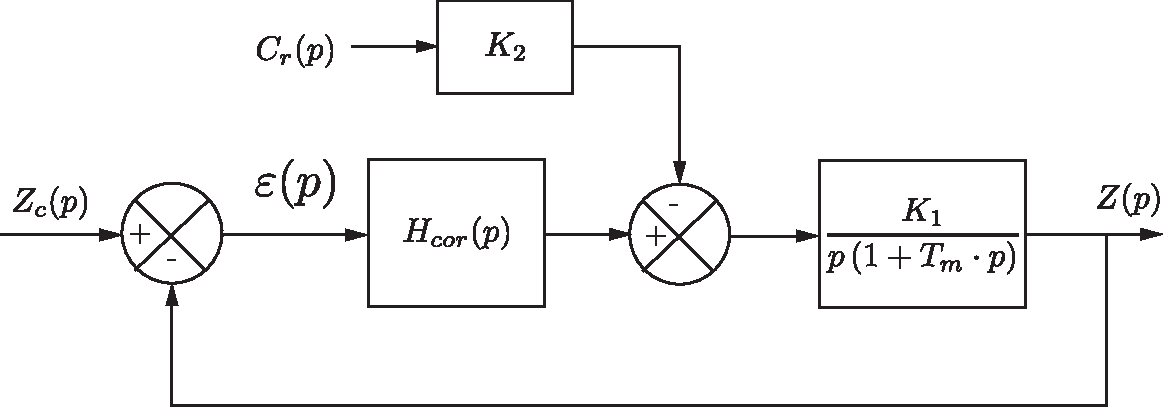
\includegraphics[width=\linewidth]{64_01}
\end{marginfigure}

\fi
 
\question{Tracer le diagramme de Bode asymptotique de $H_{\text{BO}}(p)$ pour des pulsations comprises entre \SI{0,5}{rad.s^{-1}} et \SI{50}{rad.s^{-1}}.}
\ifprof
\else 
\fi

\question{Tracer le diagramme de Bode du retard pour des pulsations comprises entre \SI{0,5}{rad.s^{-1}} et \SI{50}{rad.s^{-1}}.}
\ifprof
\else 
\fi


\ifprof
\else
On donne le diagramme de la FTBO retardée. 

\begin{marginfigure}
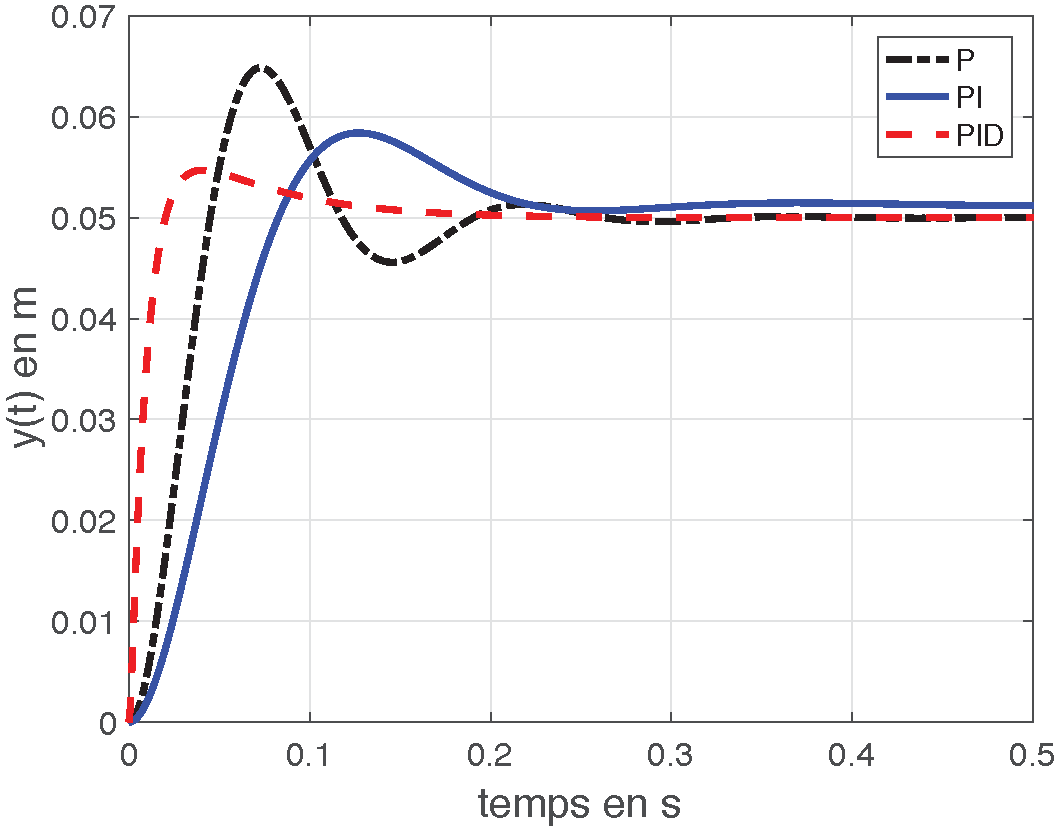
\includegraphics[width=\linewidth]{64_02}
\end{marginfigure}
\fi

\question{Déterminer le gain $K_c$ qui donne une marge de phase de 50\degres.}
\ifprof
\else 
\fi

\question{La constante $T_c$ qui laisse subsister une marge de phase d’environ 45\degres.}
\ifprof
\else 
\fi


\question{Quelle est l’erreur de traînage du système corrigé pour l’entrée en rampe considérée (en négligeant le retard).}
\ifprof
\else 
\fi


\ifprof
\else



\marginnote{Corrigé voir \ref{PERF:02:C2:03:stab:64}.}

\fi 
 
\section{Évaluer expérimentalement des grandeurs géométriques} 
\setchapterpreamble[u]{\margintoc} 
\chapter{Résoudre un problème de cinématique} 
\section{Analyser un mécanisme, justifier des choix des liaisons, réaliser un schéma cinématique paramétré} 
\graphicspath{{\repStyle/png/}{../CIN/CIN-01-ModeliserSchemasCinematiques/01_T/images/}} 
\normaltrue
\correctiontrue

%\UPSTIidClasse{11} % 11 sup, 12 spé
%\newcommand{\UPSTIidClasse}{12}


\exer{Mouvement T -- $\star$ \label{CIN:01:B2:12:01}}
\setcounter{question}{0}\marginnote{\xpComp{CIN}{01}}%\UPSTIcompetence{B2-12}
\index{Compétence B2-12}\index{Compétence CIN-01}
\index{Mécanisme à 1 translation}
\ifcorrection
\else
\marginnote{\textbf{Pas de corrigé pour cet exercice.}}
\fi

\ifprof
\else
Soit le mécanisme suivant. On note $\vect{AB}=\lambda(t)\vect{i_0}$.
\begin{marginfigure}
\includegraphics[width=\linewidth]{01_T_01}
\end{marginfigure}
\fi

\ifprof
\begin{multicols}{3}
\else
\fi
\question{Tracer le graphe des liaisons.}
\ifprof\begin{marginfigure}
\includegraphics[width=\linewidth]{01_T_01_c}
\end{marginfigure}
\else
\fi


\question{Retracer le schéma cinématique pour $\lambda=\SI{10}{mm}$.}
\ifprof
\begin{marginfigure}
\includegraphics[width=\linewidth]{01_T_02_c}
\end{marginfigure}
\else
\fi

\question{Retracer le schéma cinématique pour $\lambda=-\SI{20}{mm}$.}
\ifprof
\begin{marginfigure}
\includegraphics[width=\linewidth]{01_T_03_c}
\end{marginfigure}
\else
\fi


\ifprof
\end{multicols}
\else
\fi

\ifprof
\else

\marginnote{Corrigé  voir \ref{CIN:01:B2:12:01}.}

\fi


 
 
\graphicspath{{\repStyle/png/}{../CIN/CIN-01-ModeliserSchemasCinematiques/02_R/images/}} 
\normaltrue
\correctiontrue

%\UPSTIidClasse{11} % 11 sup, 12 spé
%\newcommand{\UPSTIidClasse}{12}

%\section{Rotation simple} %\label{CIN:01:B2:12:01}
\exer{Mouvement R  $\star$ \label{CIN:01:B2:12:02}}
\setcounter{question}{0}\marginnote{\xpComp{CIN}{01}}%\UPSTIcompetence{B2-12}
\index{Compétence B2-12}\index{Compétence CIN-01}
\index{Mécanisme à 1 rotation}
\ifcorrection
\else
\marginnote{\textbf{Pas de corrigé pour cet exercice.}}
\fi

\ifprof
\else
Soit le mécanisme suivant. On a $\vect{AB}=R\vect{i_1}$ avec $R=\SI{20}{mm}$. 
\begin{marginfigure}
\includegraphics[width=\linewidth]{02_R_01}
\end{marginfigure}
\fi


\question{Tracer le graphe des liaisons.}
\ifprof
\begin{marginfigure}
\includegraphics[width=\linewidth]{02_R_01_c}
\end{marginfigure}
\else
\fi

\question{Retracer le schéma cinématique pour $\theta=\dfrac{\pi}{4}\,\text{rad}$.}
\ifprof
\begin{marginfigure}
\includegraphics[width=.4\linewidth]{02_R_02_c}
\end{marginfigure}
\else
\fi

\question{Retracer le schéma cinématique pour $\theta={\pi}\, \text{rad}$.}
\ifprof
\begin{marginfigure}
\includegraphics[width=.8\linewidth]{02_R_03_c}
\end{marginfigure}
\else
\fi


\ifprof
\else
\marginnote{Corrigé  voir \ref{CIN:01:B2:12:02}.}
\fi 
 
\graphicspath{{\repStyle/png/}{../CIN/CIN-01-ModeliserSchemasCinematiques/03_TT/images/}} 
\normaltrue
\correctiontrue

%\UPSTIidClasse{11} % 11 sup, 12 spé
%\newcommand{\UPSTIidClasse}{11}


\exer{Mouvement TT -- $\star$ \label{C2:09:03}}
\setcounter{question}{0}\UPSTIcompetence[2]{C2-09}
\index{Compétence C2-09}
\index{Principe fondamental de la dynamique}
\index{PFD}
\index{Mécanisme à 2 translations}
\ifcorrection
\else
\marginnote{\textbf{Pas de corrigé pour cet exercice.}}
\fi

\ifprof
\else
Soit le mécanisme suivant. On note $\vect{AB}=\lambda(t)\vect{i_0}$ et $\vect{BC}=\mu(t)\vect{j_0}$.
$G_1 = B$ désigne le centre d'inertie de \textbf{1},et $m_1$ sa masse et $\inertie{G_1}{1}=\matinertie{A_1}{B_1}{C_1}{0}{0}{0}{\bas{1}}$; 
$G_2 = C$ désigne le centre d'inertie de \textbf{2} et  $m_2$ sa masse  et $\inertie{G_2}{2}=\matinertie{A_2}{B_2}{C_2}{0}{0}{0}{\bas{2}}$.

 Un vérin électrique positionné entre \textbf{0} et \textbf{1} permet d'actionner le solide \textbf{1}.
 Un vérin électrique positionné entre \textbf{1} et \textbf{2} permet d'actionner le solide \textbf{2}.

L'accélération de la pesanteur est donnée par $\vect{g}=-g\vect{j_0}$.

\begin{center}
\includegraphics[width=.6\linewidth]{03_TT_01}
\end{center}
\fi

\question{Dans le but d'obtenir les lois de mouvement, appliquer le théorème de la résultante dynamique au solide \textbf{2} en projection sur $\vect{j_0}$.}
\ifprof

On isole \textbf{2}. 

\vspace{.25cm}

Bilan des actions mécaniques : 
\begin{itemize}
\item liaison glissière entre 1 et 2 : 
$\torseurstat{T}{1}{2}= \torseurl{X_{12}\vi{0}+Z_{12}\vk{0}}{L_{12}\vi{0}+M_{12}\vj{0}+N_{12}\vk{0}}{B}$;
\item pesanteur : $\torseurstat{T}{\text{Pes}}{2}= \torseurl{-m_2 g \vj{0}}{\vect{0}}{C}$;
\item vérin : $\torseurstat{T}{1_v}{2}= \torseurl{F_2 \vj{0}}{\vect{0}}{B}$.
\end{itemize}

\vspace{.25cm}

Application du TRD au solide \textbf{2} en projection sur $\vj{0}$: 

$\vectf{1}{2}\cdot \vj{0} + \vectf{\text{Pes}}{2}\cdot \vj{0}+ \vectf{1_v}{2}\cdot \vj{0} = \vectrd{2}{0}\cdot \vj{0}$.

\vspace{.25cm}

Calcul de la résultante dynamique : 
$\vectrd{2}{0} = m_2 \vectg{C}{2}{0} = m_2 \left(\lambdapp (t) \vi{0}+\mupp (t) \vj{0}\right)$.

Application du théorème : 
$$
-m_2g  + F_2 = m_2\mupp (t).
$$
\else
\fi


\question{Dans le but d'obtenir les lois de mouvement, appliquer le théorème de la résultante dynamique à l'ensemble \textbf{1+2} en projection sur $\vect{i_0}$}
\ifprof
On isole \textbf{1+2}. 

\vspace{.25cm}

Bilan des actions mécaniques : 
\begin{itemize}
\item liaison glissière entre 0 et 1 : 
$\torseurstat{T}{0}{1}= \torseurl{Y_{01}\vj{0}+Z_{12}\vk{0}}{L_{12}\vi{0}+M_{12}\vj{0}+N_{12}\vk{0}}{A}$;
\item pesanteur : $\torseurstat{T}{\text{Pes}}{1}= \torseurl{-m_1 g \vj{0}}{\vect{0}}{B}$;
\item pesanteur : $\torseurstat{T}{\text{Pes}}{2}= \torseurl{-m_2 g \vj{0}}{\vect{0}}{C}$;
\item vérin : $\torseurstat{T}{0_v}{1}= \torseurl{F_1 \vi{0}}{\vect{0}}{B}$.
\end{itemize}

\vspace{.25cm}

Application du TRD au solide \textbf{1+2} en projection sur $\vi{0}$: 

$\vectf{0}{1}\cdot \vi{0} + \vectf{\text{Pes}}{1}\cdot \vi{0}+ \vectf{\text{Pes}}{2}\cdot \vj{0}+ \vectf{0_v}{2}\cdot \vi{0} = \vectrd{1+2}{0}\cdot \vi{0}$.

\vspace{.25cm}

Calcul de la résultante dynamique : 
$\vectrd{1+2}{0} = m_1 \vectg{B}{1}{0}+m_2 \vectg{C}{2}{0} = m_1 \lambdapp (t) \vi{0} + m_2 \left(\lambdapp (t) \vi{0}+\mupp (t) \vj{0}\right)$.

Application du théorème : 
$$
F_1  + F_2 = m_1 \lambdapp (t)  + m_2 \lambdapp (t) .
$$

\else
\fi


\ifprof
\else
\begin{flushright}
\footnotesize{Corrigé  voir \ref{C2:09:03}.}
\end{flushright}%
\fi 
 
\graphicspath{{\repStyle/png/}{../CIN/CIN-01-ModeliserSchemasCinematiques/04_RR/images/}} 
\normaltrue
\correctiontrue

%\UPSTIidClasse{11} % 11 sup, 12 spé
%\newcommand{\UPSTIidClasse}{12}

\exer{Mouvement RR  $\star$ \label{CIN:01:B2:12:04}}
\setcounter{question}{0}\marginnote{\xpComp{CIN}{01}}%\UPSTIcompetence{B2-12}
\index{Compétence B2-12}\index{Compétence CIN-01}
\index{Mécanisme à 2 rotations}
\ifcorrection
\else
\marginnote{\textbf{Pas de corrigé pour cet exercice.}}
\fi

\ifprof
\else
Soit le mécanisme suivant. On a $\vect{AB}=R\vect{i_1}$ avec $R=\SI{20}{mm}$ et  
$\vect{BC}=L\vect{i_2}$ avec $L=\SI{15}{mm}$.
\begin{marginfigure}
\includegraphics[width=\linewidth]{04_RR_01}
\end{marginfigure}
\fi

\question{Tracer le graphe des liaisons.}
\ifprof
\begin{marginfigure}
\includegraphics[width=.2\linewidth]{04_RR_01_c}
\end{marginfigure}
\else
\fi


\ifprof
\begin{multicols}{3}
\else
\fi

\question{Retracer le schéma cinématique pour $\theta=\dfrac{\pi}{4}\,\text{rad}$ et $\varphi=\pi\,\text{rad}$.}
\ifprof
\begin{marginfigure}
\includegraphics[width=\linewidth]{04_RR_02_c}
\end{marginfigure}
\else
\fi

\question{Retracer le schéma cinématique pour $\theta=\dfrac{\pi}{4}\,\text{rad}$ et $\varphi=-\dfrac{\pi}{4}\,\text{rad}$.}
\ifprof
\begin{marginfigure}
\includegraphics[width=\linewidth]{04_RR_03_c}
\end{marginfigure}
\else
\fi


\question{Retracer le schéma cinématique pour $\theta=\dfrac{3\pi}{4}\,\text{rad}$ et $\varphi=-\dfrac{\pi}{4}\,\text{rad}$.}
\ifprof
\begin{marginfigure}
\includegraphics[width=\linewidth]{04_RR_04_c}
\end{marginfigure}
\else
\fi

\ifprof
\end{multicols}
\else
\fi

\ifprof
\else

\marginnote{Corrigé  voir \ref{CIN:01:B2:12:04}.}

\fi 
 
\graphicspath{{\repStyle/png/}{../CIN/CIN-01-ModeliserSchemasCinematiques/05_RT/images/}} 
\normaltrue
\correctiontrue

%\UPSTIidClasse{11} % 11 sup, 12 spé
%\newcommand{\UPSTIidClasse}{12}

\exer{Mouvement RT  $\star$ \label{CIN:01:B2:12:05}}
\setcounter{question}{0}\marginnote{\xpComp{CIN}{01}}%\UPSTIcompetence{B2-12}
\index{Compétence B2-12}\index{Compétence CIN-01}
\index{Mécanisme à 1 rotation et 1 translation}
\ifcorrection
\else
\marginnote{\textbf{Pas de corrigé pour cet exercice.}}
\fi

\ifprof
\else
Soit le mécanisme suivant. On a $\vect{AB}=\lambda(t)\vect{i_1}$.
\begin{marginfigure}
\includegraphics[width=\linewidth]{05_RT_01}
\end{marginfigure}
\fi

\question{Tracer le graphe des liaisons.}
\ifprof
\begin{marginfigure}
\includegraphics[width=6cm]{05_RT_01_01}
\end{marginfigure}
\else
\fi

\question{Retracer le schéma cinématique pour $\theta=\dfrac{\pi}{4}\,\text{rad}$ et $\lambda(t)=\SI{20}{mm}$.}
\ifprof
\else
\fi

\question{Retracer le schéma cinématique pour $\theta=\dfrac{-\pi}{4}\,\text{rad}$ et $\lambda(t)=-\SI{20}{mm}$.}
\ifprof\begin{marginfigure}
\includegraphics[width=.8\linewidth]{05_RT_01_02}
\end{marginfigure}
\else
\fi




\ifprof
\else

\marginnote{Corrigé  voir \ref{CIN:01:B2:12:05}.}

\fi 
 
\graphicspath{{\repStyle/png/}{../CIN/CIN-01-ModeliserSchemasCinematiques/06_TR/images/}} 
\normaltrue
\correctionfalse

%\UPSTIidClasse{11} % 11 sup, 12 spé
%\newcommand{\UPSTIidClasse}{12}

\exer{Mouvement RT  $\star$ \label{B2:12:06}}
\setcounter{question}{0}\UPSTIcompetence{B2-12}
\index{Compétence B2-12}
\index{Mécanisme à 1 translation et 1 rotation}
\ifcorrection
\else
\marginnote{\textbf{Pas de corrigé pour cet exercice.}}
\fi

\ifprof
\else
Soit le mécanisme suivant. On a $\vect{AB}=\lambda(t)\vect{i_0}$ et $\vect{BC}=R\vect{i2}$.
\begin{center}
\includegraphics[width=\linewidth]{06_TR_01}
\end{center}
\fi

\question{Tracer le graphe des liaisons.}
\ifprof
\else
\fi

\question{Retracer le schéma cinématique pour $\theta=\dfrac{\pi}{4}\,\text{rad}$ et $\lambda(t)=\SI{20}{mm}$.}
\ifprof
\else
\fi

\question{Retracer le schéma cinématique pour $\theta=\dfrac{-\pi}{4}\,\text{rad}$ et $\lambda(t)=-\SI{20}{mm}$.}
\ifprof
\else
\fi



\ifprof
\else
\begin{flushright}
\footnotesize{Corrigé  voir \ref{B2:12:06}.}
\end{flushright}%
\fi 
 
\graphicspath{{\repStyle/png/}{../CIN/CIN-01-ModeliserSchemasCinematiques/07_RR3D/images/}} 
\normalfalse \difficiletrue \tdifficilefalse
\correctionfalse

%\UPSTIidClasse{11} % 11 sup, 12 spé
%\newcommand{\UPSTIidClasse}{12}

\exer{Mouvement RR 3D  $\star\star$ \label{CIN:01:B2:12:07}}
\setcounter{question}{0}\marginnote{\xpComp{CIN}{01}}%\UPSTIcompetence{B2-12}
\index{Compétence B2-12}\index{Compétence CIN-01}
\index{Mécanisme à 2 rotations 3D}
\ifcorrection
\else
\marginnote{\textbf{Pas de corrigé pour cet exercice.}}
\fi

\ifprof
\else
Soit le mécanisme suivant. On a $\vect{AB}=R\vect{i_1}$ et $\vect{BC}=\ell\vect{i_2}+r\vect{j_2}$. On note $R+\ell=L = \SI{20}{mm}$ et $r=\SI{10}{mm}$.
\begin{marginfigure}
\includegraphics[width=\linewidth]{07_RR3D_01}
\end{marginfigure}
\fi


\question{Tracer le graphe des liaisons.}
\ifprof
\else
\fi

\question{Retracer le schéma cinématique en 3D pour $\theta(t)=\dfrac{\pi}{2}\,\text{rad}$ et $\varphi(t)=\dfrac{\pi}{2}\, \text{rad}$.}
\ifprof
\else
\fi





\ifprof
\else

\marginnote{Corrigé  voir \ref{CIN:01:B2:12:07}.}

\fi 
 
\graphicspath{{\repStyle/png/}{../CIN/CIN-01-ModeliserSchemasCinematiques/08_RR3D/images/}} 
\normalfalse \difficiletrue \tdifficilefalse
\correctionfalse

%\UPSTIidClasse{11} % 11 sup, 12 spé
%\newcommand{\UPSTIidClasse}{12}

\exer{Mouvement RR 3D  $\star\star$ \label{B2:12:08}}
\setcounter{question}{0}\UPSTIcompetence{B2-12}
\index{Compétence B2-12}
\index{Mécanisme à 2 rotations 3D}
\ifcorrection
\else
\marginnote{\textbf{Pas de corrigé pour cet exercice.}}
\fi

\ifprof
\else
Soit le mécanisme suivant. On a $\vect{AB}=H\vect{j_1}+R\vect{i_1}$ et $\vect{BC}=L\vect{i_2}$. On a $H=\SI{20}{mm}$, $r=\SI{5}{mm}$, $L=\SI{10}{mm}$. 
\begin{center}
\includegraphics[width=\linewidth]{08_RR3D_01}
\end{center}
\fi

\question{Tracer le graphe des liaisons.}
\ifprof
\else
\fi

\question{Retracer le schéma cinématique en 3D pour $\theta(t)=\pi\,\text{rad}$ et $\varphi(t)=-\dfrac{\pi}{4}\, \text{rad}$.}
\ifprof
\else
\fi





\ifprof
\else
\begin{flushright}
\footnotesize{Corrigé  voir \ref{B2:12:08}.}
\end{flushright}%
\fi 
 
\graphicspath{{\repStyle/png/}{../CIN/CIN-01-ModeliserSchemasCinematiques/09_RT_RSG/images/}} 
\normalfalse \difficiletrue \tdifficilefalse
\correctionfalse

%\UPSTIidClasse{11} % 11 sup, 12 spé
%\newcommand{\UPSTIidClasse}{12}

\exer{Mouvement RT -- RSG  $\star\star$ \label{CIN:01:B2:12:09}}
\setcounter{question}{0}\marginnote{\xpComp{CIN}{01}}%\UPSTIcompetence{B2-12}
\index{Compétence B2-12}\index{Compétence CIN-01}
\index{Mécanisme à 1 rotations, 1 translation et RSG}
\ifcorrection
\else
\marginnote{\textbf{Pas de corrigé pour cet exercice.}}
\fi

\ifprof
\else
Soit le mécanisme suivant. On a $\vect{IA}=R\vect{j_0}$ et $\vect{AB}=\lambda(t)\vect{i_1}$. De plus $R=\SI{15}{mm}$.
\begin{marginfigure}
\includegraphics[width=\linewidth]{09_RT_RSG_01}
\end{marginfigure}
\fi


\question{Tracer le graphe des liaisons.}
\ifprof
\else
\fi


\question{Retracer le schéma cinématique pour $\theta(t)=0\,\text{rad}$ et $\lambda(t)=\SI{20}{mm}$. On notera $I_1$ le point de contact entre \textbf{0} et \textbf{1}.}
\ifprof
\else
\fi

\question{Retracer le schéma cinématique pour $\theta(t)=\dfrac{\pi}{2}\,\text{rad}$ et $\lambda(t)=\SI{30}{mm}$. On notera $I_2$ le point de contact entre \textbf{0} et \textbf{1}. On précisera la position des points $I_{0,0}$ et $I_{0,1}$, points résultants de la rupture de contact lors du passage de $\theta(t)$ de 0 à $\dfrac{\pi}{2}$.}
\ifprof
\else
\fi





\ifprof
\else

\marginnote{Corrigé  voir \ref{CIN:01:B2:12:09}.}

\fi 
 
\graphicspath{{\repStyle/png/}{../CIN/CIN-01-ModeliserSchemasCinematiques/1018_BorneReglable/images/}} 
\normalfalse \difficiletrue \tdifficilefalse
\correctionfalse
%\UPSTIidClasse{11} % 11 sup, 12 spé
%\newcommand{\UPSTIidClasse}{12}

\exer{Borne réglable  $\star\star$ \label{CIN:01:B2:12:1018}}
\setcounter{question}{0}\marginnote{\xpComp{CIN}{01}}%\UPSTIcompetence{B2-12}
\index{Compétence B2-12}\index{Compétence CIN-01}
\index{Schéma cinématique}

\ifcorrection
\else
\marginnote{\textbf{Pas de corrigé pour cet exercice.}}
\fi

\ifprof
\else
Soit la borne réglable suivante. 
\begin{marginfigure}
\includegraphics[width=\linewidth]{1018_01}
\end{marginfigure}
\fi


\ifprof
\else
La nomenclature est la suivante. 

\begin{marginfigure}
\begin{tabular}{lll}
\hline
\textbf{Rep} & \textbf{Désignation} & \textbf{Quantité} \\ \hline 
1 & Coulisseau & 1 \\ 
2 & Borne & 1 \\ 
3 & Corps & 1 \\ 
4 & Vis de guidage & 1 \\ 
5 & Couvercle & 1 \\ 
6 & Vis de couvercle & 2 \\ 
7 & Socle & 1 \\ 
8 & Vis de socle & 4 \\ 
10 & Molette & 1 \\ 
12 & Vis & 1 \\
13 & Goupille fendue & 1 \\ 
\hline
\end{tabular}
\end{marginfigure}
\fi


\question{Colorier le dessin de définition en utilisant la même couleur pour une même classe d'équivalence.}
\ifprof
\else
\fi

\question{Lister les classes classes d'équivalence.}
\ifprof
\else
\fi

\question{Donner le graphe de liaisons en précisant rigoureusement les liaisons. Justifier le choix des liaisons.}
\ifprof
\else
\fi


\question{Réaliser le schéma cinématique.}
\ifprof
\else
\fi

\ifprof
\else

\footnotesize
%\begin{marginfigure}
%\begin{tabular}{|p{.9\linewidth}|}
%\hline
%Indications (à vérifier...) :
%\begin{enumerate}
%\item $\vectv{B}{2}{0} = L\varphip(t)\vj{2} +\thetap(t)\left(L\vj{1}-R\vi{0}\right) $.
%\item  $\torseurcin{V}{2}{0} = \torseurl{\vecto{2}{0}=\left( \varphip(t)+\thetap(t) \right) \vk{0} }{ L\varphip(t)\vj{2} +\thetap(t)\left(L\vj{1}-R\vi{0}\right)}{B}$.
%\item $\vectg{B}{2}{0} =  L\varphipp(t)\vj{2}-L\varphip(t)\left(\varphip(t)+\thetap(t) \right)\vi{2}  + \thetapp(t)\left(L\vj{1}-R\vi{0}\right) - L\thetap^2(t)\vi{1}$.
%\end{enumerate} \\ \hline
%\end{tabular}
%\end{marginfigure}
\normalsize



\marginnote{Corrigé  voir \ref{CIN:01:B2:12:1018}.}

\fi 
 
\graphicspath{{\repStyle/png/}{../CIN/CIN-01-ModeliserSchemasCinematiques/1019_RobotPeinture/images/}} 
\normalfalse \difficiletrue \tdifficilefalse
\correctionfalse
%\UPSTIidClasse{11} % 11 sup, 12 spé
%\newcommand{\UPSTIidClasse}{12}

\exer{Robot de toit  $\star\star$ \label{B2:12:1019}}
\setcounter{question}{0}\UPSTIcompetence{B2-12}
\index{Compétence B2-12}
\index{Schéma cinématique}

\ifcorrection
\else
\marginnote{\textbf{Pas de corrigé pour cet exercice.}}
\fi

\ifprof
\else
Soit le mécanisme donné au verso.
\fi


\ifprof
\else
La nomenclature est la suivante. 
\begin{multicols}{2}
\begin{center}
\begin{tabular}{|l|l|l|}
\hline
Rep & Nb  & Désignation \\ \hline \hline % & Matière \\ \hline \hline
1 & 1 & Carter inférieur fixe  \\ \hline %&  Al Si 13 \\ \hline 
2&
1&
Carter supérieur pivotant\\ \hline %& Al Si 13 \\ \hline 
3&
2 &
Ecrou hexagonal ISO 4032 - M10 \\ \hline %& \\ \hline 
4&
1&
Rondelle plate ISO 10673 – Type N - 10 \\ \hline %& \\ \hline 
5&
1&
Axe fileté à tête fendu \\ \hline %& \\ \hline 
6&
1&
Plat de fermeture%&
\\ \hline %S 235 \\ \hline 
7&
7&
Rondelle plate ISO 10673 -- Type N - 5 \\ \hline %& \\ \hline 
8&
1&
Bride de liaison support coussinets \\ \hline % &Al Cu 4 Mg Si \\ \hline 
9&
1&
Bride de liaison gauche \\ \hline % & Al Cu 4 Mg Si   \\ \hline 
10&
2&
Coussinet \\ \hline %& Cu Sn 12 P  \\ \hline 
11&
1&
Tube carter \\ \hline %& \\ \hline 
12&
1&
Bride de liaison droite \\ \hline %& Al Cu 4 Mg Si \\ \hline 
13&
1&
Carter cylindrique\\ \hline % & \\ \hline 
14&
1&
Axe excentré \\ \hline %& \\ \hline 
15&
4&
Vis à tête cylindrique à six pans creux\\ \hline % ISO 4762 - M5-50\\ \hline % & \\ \hline 
16&
1&
Chape mâle\\ \hline % & C 45 \\ \hline 
17&
2&
Goupille cylindrique \\ \hline %ISO 8734 - 2x16 \\ \hline %& \\ \hline 
18&
1&
Bielle rotule \\ \hline % &C 45 \\ \hline 
19&
1&
Cale de réglage \\ \hline %& \\ \hline 
20&
1&
Fermeture rotule \\ \hline %& \\ \hline 
21&
1&
Bielle à portée sphérique \\ \hline %& \\ \hline 
22&
3&
Vis à tête cylindrique à six pans creux  \\
&& ISO 4762 - M5-30 \\ \hline %& \\ \hline 
23&
1&
Goupille cylindrique ISO 8734 - 3x30  \\ \hline %& \\ \hline 
24&
1&
Chape femelle \\ \hline %& \\ \hline %C 45 \\ \hline 

25&
1&
Axe de chape \\ \hline % & \\ \hline 
26&
1&
Anneau élastique pour arbre, 4 x 0,4 \\ \hline % & \\ \hline 
27&
2&
Coussinet à collerette \\ \hline %& Cu Sn 12 P \\ \hline 
28&
1&
Bielle \\ \hline % & C 45 \\ \hline 
\end{tabular}
\end{center}

\begin{center}
\begin{tabular}{|l|l|l|}
\hline
Rep & Nb  & Désignation \\ \hline \hline % & Matière \\ \hline \hline
29&
3&
Vis à tête cylindrique à six pans creux \\ \hline % ISO 4762 - M5-18 \\ \hline % & \\ \hline 
30&
1&
Axe d'articulation \\ \hline % & \\ \hline 
31&
1&
Axe de sortie \\ \hline % & \\ \hline %100 Cr 6  \\ \hline 
32&
1&
Support d'axe de sortie \\ \hline %C 45 \\ \hline 
33&
1&
Ecrou hexagonal \\ \hline % ISO 4032 - M24  \\ \hline %& \\ \hline 
34&
1&
Rondelle plate \\ \hline % ISO 10673 – Type S - 24\\ \hline % &  \\ \hline 
35&
2&
Coussinet à collerette \\ \hline %& Cu Sn 12 P  \\ \hline 
36&
1&
Plateau support excentrique \\ \hline %& \\ \hline 
37&
1&
Vis à tête moletée \\ \hline %& \\ \hline 
38&
1&
Doigt de réglage \\ \hline % & C 22 \\ \hline 
39&
1&
Coussinet \\ \hline %& Cu Sn 12 P \\ \hline 
40&
1&
Entretoise  \\ \hline 
41&
2&
Anneau élastique pour arbre, 6 x 0,7  \\ \hline %& \\ \hline 
42&
1&
Anneau élastique pour alésage, 32 x 1,5 \\ \hline %& \\ \hline 
43&
1&
Anneau élastique pour arbre, 12 x 1 \\ \hline %& \\ \hline 
44&
1&
Arbre d’entrée \\ \hline %& \\ \hline 
45&
2&
Roulement à une rangée de \\ 
&& billes à contact radial \\ \hline %& \\ \hline 
46&
1&
Support roulements \\ \hline %& Al Cu 4 Mg Si \\ \hline 
47&
1&
Carter \\ \hline % & Al Cu 4 Mg Si \\ \hline 
48&
1&
Vis sans fin Z48 = 2 filets \\ \hline %& \\ \hline 
49&
2&
Boitier\\ \hline % & \\ \hline 
50&
2&
Roulement à une rangée de \\ 
&& billes à contact radial\\  \hline % & \\ \hline 
51&
2&
Joint à deux lèvres \\ \hline %& \\ \hline 
52&
1&
Arbre Creux\\ \hline % & \\ \hline
53&
1&
Vis à tête hexagonale ISO 4014-M6 \\ \hline %  & \\ \hline 
54 & 
1 &
Arbre \\ \hline % & \\ \hline 
55 &
1&
Roue dentée Z55= 60 dents  \\ \hline %&Cu Ni 2 Si  \\ \hline 
\end{tabular}
\end{center}

\end{multicols}

\fi

\question{Colorier le dessin de définition en utilisant la même couleur pour une même classe d'équivalence.}
\ifprof
\else
\fi

\question{Lister les classes classes d'équivalence.}
\ifprof
\else
\fi

\question{Donner le graphe de liaisons en précisant rigoureusement les liaisons. Justifier le choix des liaisons.}
\ifprof
\else
\fi


\question{Réaliser le schéma cinématique.}
\ifprof
\else
\fi


\ifprof
\else
\begin{center}
\includegraphics[width=\linewidth]{1019_01}
\end{center}
\fi


\ifprof
\else

\footnotesize
%\begin{center}
%\begin{tabular}{|p{.9\linewidth}|}
%\hline
%Indications (à vérifier...) :
%\begin{enumerate}
%\item $\vectv{B}{2}{0} = L\varphip(t)\vj{2} +\thetap(t)\left(L\vj{1}-R\vi{0}\right) $.
%\item  $\torseurcin{V}{2}{0} = \torseurl{\vecto{2}{0}=\left( \varphip(t)+\thetap(t) \right) \vk{0} }{ L\varphip(t)\vj{2} +\thetap(t)\left(L\vj{1}-R\vi{0}\right)}{B}$.
%\item $\vectg{B}{2}{0} =  L\varphipp(t)\vj{2}-L\varphip(t)\left(\varphip(t)+\thetap(t) \right)\vi{2}  + \thetapp(t)\left(L\vj{1}-R\vi{0}\right) - L\thetap^2(t)\vi{1}$.
%\end{enumerate} \\ \hline
%\end{tabular}
%\end{center}
\normalsize


\begin{flushright}
\footnotesize{Corrigé  voir \ref{B2:12:1018}.}
\end{flushright}%
\fi 
 
\graphicspath{{\repStyle/png/}{../CIN/CIN-01-ModeliserSchemasCinematiques/1020_PompeEnsieta/images/}} 
\normalfalse \difficiletrue \tdifficilefalse
\correctionfalse
%\UPSTIidClasse{11} % 11 sup, 12 spé
%\newcommand{\UPSTIidClasse}{12}

\exer{Pompe ENSIETA  $\star\star$ \label{E2:05:1020}}
\setcounter{question}{0}\UPSTIcompetence{E2-05}
\index{Compétence E2-05}
\index{Dessin de définition}
\index{Pompe ENSIETA}

\ifcorrection
\else
\marginnote{\textbf{Pas de corrigé pour cet exercice.}}
\fi


\ifprof
\else
Le plan joint format A4 représente l’ensemble monté d’une pompe hydraulique manuelle.

La pompe est fixée sur un support vertical au moyen de 3 trous filetés (1). Une série de trois trous filetés est usinée sur chaque coté du corps (2), permettant ainsi de fixer indifféremment la pompe sur l’une ou l’autre de ses faces.

L’admission de l’huile est effectuée par l’orifice (3), le refoulement par l’orifice (4).

Le pompage s’effectue en actionnant un levier placé dans l’alésage cannelé du maneton (5). Le mouvement alternatif est, par l’intermédiaire de la biellette articulée, transmis au piston coulissant (6).

Lors du mouvement de droite à gauche du piston coulissant, un volume d’huile est aspiré à travers (3) et vient s’emmagasiner dans l’alésage à droite de la tête du piston, simultanément l’huile qui se trouve à gauche de la tête du piston est refoulée par l’orifice (4).

Lors du mouvement de gauche à droite du piston coulissant s’effectue le transfert, à travers de la tête du piston, de l’huile emmagasinée à sa droite (celle-ci passant côté tige). Simultanément une partie de l’huile transférée est refoulée dans (4).

Un clapet anti-retour est constitué d’une bille et d’un ressort. Sur la pompe étudiée ils sont au nombre de trois. 
Le passage du fluide dans un sens, par action sur la bille provoque l’écrasement du ressort et libère le passage. 
Dans le sens contraire l’action du fluide se conjugue avec celle du ressort et interdit le passage. 
\fi

\question{Le diamètre nominal de la bille contenue dans le clapet anti-retour situé sur l’orifice (4) est identique à celui de l’alésage qui la guide. Est-ce fonctionnellement correct ? Justifier votre réponse. L’observation de la pièce (7) du clapet situé sur l’orifice (3) peut vous aider pour la réponse.}

\question{L’alésage du corps contenant l’extrémité du raccord orifice (4) et l’alésage sur lequel le piston (6) coulisse doivent-ils être réalisés avec le même type d’état de surface ? Justifier votre réponse.}

\question{Entre la tige du piston et l’alésage du corps, quel ajustement choisir ? Préciser s’il s’agit d’un ajustement avec jeu, avec serrage ou ajusté.}

\question{D’après la représentation du dessin d’ensemble, un des composants de la pompe ne peut pas être monté. Quel est-il (donner son numéro) ? Pourquoi ? Que faudrait-il faire pour le rendre montable ?}

\question{Dans le mouvement de droite à gauche du piston, le volume aspiré dans (3) à droite de la tête de piston est-il le même que celui refoulé à gauche de la tête de piston dans (4) ? Justifier votre réponse.}


\ifprof
\else
On donne les dimensions suivantes :
\begin{itemize}
\item tête de piston = \SI{29}{mm};
\item tige de piston = \SI{18}{mm};
\item course du piston = \SI{31}{mm}.
\end{itemize}
\fi

\question{Quel est le volume d’huile  envoyé à la sortie (4) :}
\textit{
\begin{itemize}
\item lors de la course droite -- gauche du piston ?
\item lors de la course gauche -- droite du piston ?
\end{itemize}}
%
%
%
%\subsection*{Schéma cinématique}
%On considère la pompe sans aucun clapet. Seule la transformation de mouvement permettant le déplacement du piston nous intéresse.
%
%\question{Faire le schéma cinématique de la pompe.}


\ifprof
\else
\subsection*{Travail graphique}
Le corps (2) est représenté en image de synthèse sous plusieurs angles.


\begin{center}
\includegraphics[width=\linewidth]{1020_01}
\end{center}
\fi

\question{Compléter le dessin du corps (2) sur le document pré-imprimé.}


\ifprof
\else
\begin{center}
\includegraphics[width=\linewidth]{1020_02}
\end{center}
\begin{center}
\includegraphics[width=\linewidth]{1020_03}
\end{center}

\fi

\ifprof
\else

\footnotesize
%\begin{center}
%\begin{tabular}{|p{.9\linewidth}|}
%\hline
%Indications (à vérifier...) :
%\begin{enumerate}
%\item $\vectv{B}{2}{0} = L\varphip(t)\vj{2} +\thetap(t)\left(L\vj{1}-R\vi{0}\right) $.
%\item  $\torseurcin{V}{2}{0} = \torseurl{\vecto{2}{0}=\left( \varphip(t)+\thetap(t) \right) \vk{0} }{ L\varphip(t)\vj{2} +\thetap(t)\left(L\vj{1}-R\vi{0}\right)}{B}$.
%\item $\vectg{B}{2}{0} =  L\varphipp(t)\vj{2}-L\varphip(t)\left(\varphip(t)+\thetap(t) \right)\vi{2}  + \thetapp(t)\left(L\vj{1}-R\vi{0}\right) - L\thetap^2(t)\vi{1}$.
%\end{enumerate} \\ \hline
%\end{tabular}
%\end{center}
\normalsize


\begin{flushright}
\footnotesize{Corrigé  voir \ref{E2:05:1020}.}
\end{flushright}%
\fi 
 
\graphicspath{{\repStyle/png/}{../CIN/CIN-01-ModeliserSchemasCinematiques/10_PompePalette/images/}} 
\normaltrue \difficilefalse \tdifficilefalse
\correctionfalse
%\UPSTIidClasse{11} % 11 sup, 12 spé
%\newcommand{\UPSTIidClasse}{12}

\exer{Pompe à palettes  $\star$ \label{CIN:01:B2:13:PTSI:10}}
\setcounter{question}{0}\marginnote{\xpComp{CIN}{01}}%\UPSTIcompetence[2]{B2-13}
\index{Compétence B2-13-PTSI}
\index{Pompe à palettes}
\ifcorrection
\else
\marginnote{\textbf{Pas de corrigé pour cet exercice.}}
\fi

\ifprof
\else
Soit le mécanisme suivant.
\begin{marginfigure}
\includegraphics[width=.65\linewidth]{10_01}
\end{marginfigure}

\fi


\question{Réaliser le paramétrage du mécanisme.}

\ifprof

\else
\fi


\ifprof
\else
\footnotesize
\ifcolle
\else

\fi

\normalsize
\marginnote{Corrigé voir \ref{CIN:01:B2:13:PTSI:10}.}

\fi 
 
\graphicspath{{\repStyle/png/}{../CIN/CIN-01-ModeliserSchemasCinematiques/11_PompePistonsRadiaux/images/}} 
\normaltrue \difficilefalse \tdifficilefalse
\correctiontrue

%\UPSTIidClasse{11} % 11 sup, 12 spé
%\newcommand{\UPSTIidClasse}{12}

\exer{Pompe à piston axial $\star$ \label{B2:13:11}}
\setcounter{question}{0}\UPSTIcompetence[2]{B2-13}
\index{Compétence B2-13}
\index{Pompe à piston axial}
\index{Arbre à cames}
\ifcorrection
\else
\marginnote{\textbf{Pas de corrigé pour cet exercice.}}
\fi

\ifprof
\else
Soit le mécanisme suivant. On a $\vect{AB}=e\vect{i_1}$ et $\vect{BI}=R\vect{j_0}$. De plus, 
$e=\SI{10}{mm}$ et $R=\SI{20}{mm}$. Le contact entre \textbf{1} et \textbf{2} en $B$ est maintenu en permanence par un ressort suffisamment raide (non représenté) positionné entre \textbf{0} et \textbf{2}. 
\begin{center}
\includegraphics[width=\linewidth]{11_01}
\end{center}
\fi

Il est possible de mettre la loi entrée-sortie sous la forme $ \lambda(t) = e\sin\theta +R $
ou encore $\lambdap (t)=e\thetap(t) \cos\theta (t)$  (voir exercice \ref{C2:06:11}).


\question{Donner le torseur cinématique $\torseurcin{V}{2}{0}$ au point $C$.}
\ifprof
$\torseurcin{V}{2}{0} = \torseurl{\vect{0}}{\lambdap (t)\vj{0}}{C}$.
\else
\fi

\question{Déterminer $\vectg{C}{2}{0}$.}
\ifprof
$\vectg{C}{2}{0} = \lambdapp (t)\vj{0}$.
\else
\fi

\ifprof
\else
\footnotesize
\ifcolle
\else
\begin{center}
\begin{tabular}{|p{.9\linewidth}|}
\hline
Indications :
\begin{enumerate}
\item $\torseurcin{V}{2}{0} = \torseurl{\vect{0}}{\lambdap (t)\vj{0}}{C}$.
\item $\vectg{C}{2}{0} = \lambdapp (t)\vj{0}$.
\end{enumerate} \\ \hline
\end{tabular}
\end{center}
\fi
\normalsize
\begin{flushright}
\footnotesize{Corrigé  voir \ref{B2:13:11}.}
\end{flushright}%
\fi 
 
\graphicspath{{\repStyle/png/}{../CIN/CIN-01-ModeliserSchemasCinematiques/12_BielleManivelle/images/}} 
\normalfalse \difficiletrue \tdifficilefalse
\correctionfalse

%\UPSTIidClasse{11} % 11 sup, 12 spé
%\newcommand{\UPSTIidClasse}{12}

\exer{Système bielle manivelle  $\star\star$ \label{CIN:01:B2:12:12}}
\setcounter{question}{0}\marginnote{\xpComp{GEO}{01}}%\UPSTIcompetence{B2-12}
\index{Compétence B2-12}\index{Compétence CIN-01}
\index{Bielle Manivelle}
\index{Moteur}
\ifcorrection
\else
\marginnote{\textbf{Pas de corrigé pour cet exercice.}}
\fi

\ifprof
\else
Soit le mécanisme suivant. On a $\vect{AB}=R\vect{i_1}$ et $\vect{CB}=L\vect{i_2}$. De plus, 
$R=\SI{10}{mm}$ et $L=\SI{20}{mm}$. 

\begin{marginfigure}
\includegraphics[width=\linewidth]{12_01}
\end{marginfigure}
\fi

\question{Tracer le graphe des liaisons.}
\ifprof
\else
\fi

\question{Retracer le schéma cinématique pour $\theta(t)=\dfrac{\pi}{2}\,\text{rad}$.}
\ifprof
\else
\fi

\question{Retracer le schéma cinématique pour $\theta(t)=-\dfrac{\pi}{2}\,\text{rad}$.}
\ifprof
\else
\fi


\question{En déduire la course de la pièce \textbf{3}.}
\ifprof
\else
\fi



\ifprof
\else
\marginnote{Corrigé  voir \ref{CIN:01:B2:12:12}.}
\fi 
 
\graphicspath{{\repStyle/png/}{../CIN/CIN-01-ModeliserSchemasCinematiques/13_TransfoMouvement/images/}} 
\normaltrue \difficilefalse \tdifficilefalse
\correctionfalse

%\UPSTIidClasse{11} % 11 sup, 12 spé
%\newcommand{\UPSTIidClasse}{12}

\exer{Pompe oscillante $\star$ \label{C2:09:13}}
\setcounter{question}{0}\UPSTIcompetence[2]{C2-09}
\index{Compétence C2-09}
\index{TEC}
\index{Théorème de l'énergie cinétique}
\index{Pompe oscillante}

\ifcorrection
\else
\marginnote{\textbf{Pas de corrigé pour cet exercice.}}
\fi

\ifprof
\else
Soit le mécanisme suivant. On a $\vect{AB}=R\vect{i_1}$ et $\vect{CA}=H\vect{j_0}$. De plus, 
$R=\SI{10}{mm}$ et $H=\SI{60}{mm}$. Par ailleurs, on note $\vect{CB}=\lambda(t) \vect{i_2}$.
De plus, on note :
\begin{itemize}
\item $G_1$ le centre d'inertie du solide \textbf{1} tel que $\vect{AG_1}=\dfrac{R}{2} \vi{1}$, $m_1$ sa masse et $\inertie{G_1}{1}=\matinertie{A_1}{B_1}{C_1}{0}{0}{0}{\rep{1}}$ sa matrice d'inertie;
\item $G_2$ le centre d'inertie du solide \textbf{2} tel que $\vect{CG_2}=\ell \vi{2}$, $m_2$ sa masse et $\inertie{G_2}{2}=\matinertie{A_2}{B_2}{C_2}{0}{0}{0}{\rep{2}}$ sa matrice d'inertie;
\item $G_3$ le centre d'inertie du solide \textbf{3} tel que $\vect{BG_3}=-a \vi{2}$, $m_3$ sa masse et $\inertie{G_3}{2}=\matinertie{A_3}{B_3}{C_3}{0}{0}{0}{\rep{3}}$ sa matrice d'inertie.
\end{itemize}
On note $C_m\vk{0}$ le couple moteur agissant sur le solide \textbf{2}, $F_h\vi{2}$ l'action du fluide sur \textbf{3} (le fluide agissant sur le solides  \textbf{2} et \textbf{3}). L'accélération de la pesanteur est donnée par $\vect{g}=-g\vj{0}$.

\begin{center}
\includegraphics[width=\linewidth]{13_01}
\end{center}
\fi

On rappelle que la loi entrée sortie est donnée par la relation *** établie à l'exercice \ref{C2:06:13}.

\question{Tracer le graphe d'analyse en indiquant l'ensemble des actions mécaniques agissant sur les différents solides.}
\ifprof
\else
\fi

\question{Déterminer l'ensemble des puissances intérieures à l'ensemble \textbf{1+2+3}.}
\ifprof
\else
\fi

\question{Déterminer l'ensemble des puissances extérieures à l'ensemble \textbf{1+2+3}.}
\ifprof
\else
\fi

\question{Déterminer $\ec{1+2+3}{0}$.}
\ifprof
\else
\fi

\question{Déterminer la loi de mouvement en appliquant le théorème de l'énergie cinétique.}
\ifprof
\else
\fi


\ifprof
\else
\begin{flushright}
\footnotesize{Corrigé  voir \ref{C2:09:13}.}
\end{flushright}%
\fi 
 
\graphicspath{{\repStyle/png/}{../CIN/CIN-01-ModeliserSchemasCinematiques/14_Sympact/images/}} 
\normalfalse \difficiletrue \tdifficilefalse
\correctiontrue

%\UPSTIidClasse{11} % 11 sup, 12 spé
%\newcommand{\UPSTIidClasse}{12}

\exer{Barrière Sympact $\star\star$ \label{CIN:01:B2:12:14}}
\setcounter{question}{0}\marginnote{\xpComp{CIN}{01}}%\UPSTIcompetence{B2-12}
\index{Compétence B2-12}\index{Compétence CIN-01}
\index{Barrière Sympact}
\ifcorrection
\else
\marginnote{\textbf{Pas de corrigé pour cet exercice.}}
\fi

\ifprof
\else
Soit le mécanisme suivant. On a $\vect{AC}=H\vect{j_0}$ et $\vect{CB}=R\vect{i_1}$. De plus, 
$H=\SI{120}{mm}$ et $R=\SI{40}{mm}$. 

\begin{marginfigure}
\includegraphics[width=\linewidth]{14_01}
\end{marginfigure}
\fi


\question{Tracer le graphe des liaisons.}
\ifprof
\begin{marginfigure}
\includegraphics[width=.4\linewidth]{14_02_c}
\end{marginfigure}
\else
\fi

\question{Retracer le schéma cinématique pour $\theta(t)=\dfrac{\pi}{2}\,\text{rad}$.}
\ifprof
\begin{marginfigure}
\includegraphics[width=.5\linewidth]{14_01_c}
\end{marginfigure}

\else
\fi

\question{Retracer le schéma cinématique pour $\theta(t)=75\degres$.}
\ifprof
\else
\fi


\question{Dans l'hypothèse où la pièce \textbf{1} peut faire des tours complets, quelle doit être la longueur minimale de la pièce \textbf{2}.}
\ifprof
Dans cas, dans le pire des cas, $A$, $B$ et $C$ sont alignés (avec $B$ au-dessus de $C$). Il faut donc $AB = AC+CB = \SI{160}{mm}$.
\else
\fi

\question{Dans l'hypothèse où la pièce \textbf{2} fait \SI{12}{cm}, quel sera le débattement maximal de la pièce \textbf{1}.}
\ifprof
Comme je suis paresseux, j'ai réalisé la construction avec geogebra. On mesure \SI{160,8}{\degres}.
\begin{marginfigure}
\rotatebox{90}{\includegraphics[width=.35\linewidth]{14_03_c}}
\end{marginfigure}
\else
\fi

\ifprof
\else
\ifcolle
\else
\marginnote{
\begin{solution}
\begin{enumerate}
\item .
\item .
\item .
\item \SI{160}{mm}.
\item \SI{160,8}{\degres}.
\end{enumerate}
\end{solution}
\fi
Corrigé  voir \ref{CIN:01:B2:12:14}.}
\fi 
 
\graphicspath{{\repStyle/png/}{../CIN/CIN-01-ModeliserSchemasCinematiques/15_SympactGalet/images/}} 
\normalfalse \difficiletrue \tdifficilefalse
\correctionfalse

%\UPSTIidClasse{11} % 11 sup, 12 spé
%\newcommand{\UPSTIidClasse}{12}

\exer{Barrière Sympact $\star\star$ \label{B2:12:14}}
\setcounter{question}{0}\UPSTIcompetence[2]{B2-13}
\index{Compétence B2-13}
\index{Barrière Sympact}
\ifcorrection
\else
\marginnote{\textbf{Pas de corrigé pour cet exercice.}}
\fi
\ifprof
\else
Soit le mécanisme suivant. On a $\vect{AC}=H\vect{j_0}$ et $\vect{CB}=R\vect{i_1}$. De plus, 
$H=\SI{120}{mm}$, $R=\SI{40}{mm}$ $BI=\SI{10}{mm}$.

\begin{center}
\includegraphics[width=\linewidth]{15_01}
\end{center}
\fi


Il est possible de mettre la loi entrée-sortie sous la forme *** (voir exercice \ref{C2:06:14}).

\question{En utilisant la condition de roulement sans glissement au point $I$, déterminer $\gamma(t)$ et $\dot{\gamma}(t)$.}
\ifprof
\else
\fi

\question{Donner le torseur cinématique $\torseurcin{V}{3}{2}$ au point $B$.}
\ifprof
\else
\fi


\ifprof
\else
\begin{flushright}
\footnotesize{Corrigé  voir \ref{B2:12:14}.}
\end{flushright}%
\fi 
 
\graphicspath{{\repStyle/png/}{../CIN/CIN-01-ModeliserSchemasCinematiques/16_Poussoir/images/}} 
\normalfalse \difficiletrue \tdifficilefalse
\correctionfalse

%\UPSTIidClasse{11} % 11 sup, 12 spé
%\newcommand{\UPSTIidClasse}{12}

\exer{Poussoir $\star\star$ \label{CIN:01:B2:12:16}}
\setcounter{question}{0}\marginnote{\xpComp{CIN}{01}}%\UPSTIcompetence{B2-12}
\index{Compétence B2-12}\index{Compétence CIN-01}
%\index{Barrière Sympact}
\ifcorrection
\else
\marginnote{\textbf{Pas de corrigé pour cet exercice.}}
\fi

\ifprof
\else
Soit le mécanisme suivant. On a $\vect{AC}=L\vect{i_0}+H\vect{j_0}$. De plus, 
$H=\SI{120}{mm}$, $L=\SI{40}{mm}$.

\begin{marginfigure}
\includegraphics[width=\linewidth]{16_01}
\end{marginfigure}
\fi


\question{Tracer le graphe des liaisons.}
\ifprof
\else
\fi


\question{Retracer le schéma cinématique pour $\theta(t)=\dfrac{\pi}{4}\,\text{rad}$.}
\ifprof
\else
\fi

\question{Retracer le schéma cinématique pour $\theta(t)=-\dfrac{\pi}{4}\,\text{rad}$.}
\ifprof
\else
\fi


%\question{En déduire la course de la pièce \textbf{3}.}
%\ifprof
%\else
%\fi



\ifprof
\else

\marginnote{Corrigé  voir \ref{CIN:01:B2:12:16}.}

\fi 
 
\graphicspath{{\repStyle/png/}{../CIN/CIN-01-ModeliserSchemasCinematiques/17_4Barres/images/}} 
\normalfalse \difficilefalse \tdifficiletrue
\correctionfalse

%\UPSTIidClasse{11} % 11 sup, 12 spé
%\newcommand{\UPSTIidClasse}{12}

\exer{Système 4 barres $\star\star$ \label{C2:09:17}} 
\setcounter{question}{0}\UPSTIcompetence[2]{C2-09}
\index{Compétence C2-09}
\index{TEC}
\index{Théorème de l'énergie cinétique}
\index{Système 4 barres}
\index{Portail}
\ifcorrection
\else
\marginnote{\textbf{Pas de corrigé pour cet exercice.}}
\fi

\ifprof
\else
On a : 
%\begin{multicols}{2}
\begin{itemize}
\item $\vect{OA} = a \vx{1}-f \vy{1}$ avec $a=\SI{355}{mm}$ et $f=\SI{13}{mm}$;
\item $\vect{AB} = b \vx{2}$ avec $b=\SI{280}{mm}$;
\item $\vect{BC} = -c \vx{3}$ avec $c=\SI{280}{mm}$;
\item $\vect{OC} = -d \vx{0}-e\vy{0}$ avec $d=\SI{89,5}{mm}$ et $e=\SI{160}{mm}$.
\end{itemize}
De plus, on note :
\begin{itemize}
\item $G_1$ le centre d'inertie du solide \textbf{1} tel que $\vect{OG_1}=L \vx{1}$, $m_1$ sa masse et $\inertie{G_1}{1}=\matinertie{A_1}{B_1}{C_1}{0}{0}{0}{\rep{1}}$ sa matrice d'inertie;
\item $G_2$ le centre d'inertie du solide \textbf{2} tel que $\vect{AG_2}=\dfrac{b}{2}\vx{2}$, $m_2$ sa masse et $\inertie{G_2}{2}=\matinertie{A_2}{B_2}{C_2}{0}{0}{0}{\rep{2}}$ sa matrice d'inertie;
\item $G_3$ le centre d'inertie du solide \textbf{3} tel que $\vect{CG_3}=\dfrac{c}{2}\vx{3}$, $m_3$ sa masse et $\inertie{G_3}{3}=\matinertie{A_3}{B_3}{C_3}{0}{0}{0}{\rep{3}}$ sa matrice d'inertie.
\end{itemize}
On note $C_m\vk{0}$ le couple moteur agissant sur le solide \textbf{1}. L'accélération de la pesanteur est donnée par $\vect{g}=-g\vz{0}$.
%\end{multicols}
%a,b,c,d,e,ff = 355,280,280,89.5,160,13

\begin{center}
\includegraphics[width=\linewidth]{17_01}

\includegraphics[width=\linewidth]{17_02}
\end{center}
\fi
On rappelle que la loi entrée sortie est donnée par la relation *** établie à l'exercice \ref{C2:06:17}.

\question{Tracer le graphe d'analyse en indiquant l'ensemble des actions mécaniques agissant sur les différents solides.}
\ifprof
\else
\fi

\question{Déterminer l'ensemble des puissances intérieures à l'ensemble \textbf{1+2+3}.}
\ifprof
\else
\fi

\question{Déterminer l'ensemble des puissances extérieures à l'ensemble \textbf{1+2+3}.}
\ifprof
\else
\fi

\question{Déterminer $\ec{1+2+3}{0}$.}
\ifprof
\else
\fi

\question{Déterminer la loi de mouvement en appliquant le théorème de l'énergie cinétique.}
\ifprof
\else
\fi


\ifprof
\else
\begin{flushright}
\footnotesize{Corrigé  voir \ref{C2:09:17}.}
\end{flushright}%
\fi 
 
\graphicspath{{\repStyle/png/}{../CIN/CIN-01-ModeliserSchemasCinematiques/18_Maxpid/images/}} 
\normalfalse \difficilefalse \tdifficiletrue
\correctionfalse

%\UPSTIidClasse{11} % 11 sup, 12 spé
%\newcommand{\UPSTIidClasse}{12}

\exer{Maxpid $\star\star\star$ \label{B2:13:18}}
\setcounter{question}{0}\UPSTIcompetence{B2-13}
\index{Compétence B2-13}
\index{Maxpid}
\ifcorrection
\else
\marginnote{\textbf{Pas de corrigé pour cet exercice.}}
\fi

\ifprof
\else

Soit le schéma suivant. 
\begin{center}
\includegraphics[width=\linewidth]{18_01}
\end{center}
\fi

Par ailleurs $a=\SI{107,1}{mm}$, $b=\SI{80}{mm}$, $c=\SI{70}{mm}$, $d=\SI{80}{mm}$. Le pas de la vis est de $\SI{4}{mm}$.


Il est possible de mettre la loi entrée-sortie sous la forme *** (voir exercice \ref{C2:06:18}).

On définit le point $G$ tel que $\vect{OG}=L\vect{x_4}$.

\question{Donner le torseur cinématique $\torseurcin{V}{4}{0}$ au point $G$.}
\ifprof
\else
\fi

\question{Déterminer $\vectg{G}{4}{0}$.}
\ifprof
\else
\fi


\ifprof
\else
\begin{flushright}
\footnotesize{Corrigé  voir \ref{B2:13:18}.}
\end{flushright}%
\fi 
 
\graphicspath{{\repStyle/png/}{../CIN/CIN-01-ModeliserSchemasCinematiques/46_RR_RSG/images/}} 
\normalfalse \difficiletrue \tdifficilefalse
\correctiontrue

%\UPSTIidClasse{11} % 11 sup, 12 spé
%\newcommand{\UPSTIidClasse}{12}

\exer{Mouvement RR -- RSG  $\star\star$ \label{B2:13:46}}
\setcounter{question}{0}\marginnote{\UPSTIcompetence{B2-13}}
\index{Compétence B2-13}
\index{Mécanisme à 2 rotations et RSG}
\index{Segway}
\ifcorrection
\else
\marginnote{\textbf{Pas de corrigé pour cet exercice.}}
\fi

\ifprof
\else
Soit le mécanisme suivant. On a $\vect{IA}=R\vect{j_0}$ et $\vect{AB}=L\vect{i_2}$. De plus $R=\SI{15}{mm}$. On fait l'hypothèse de roulement sans glissement au point $I$.
\begin{center}
\includegraphics[width=.8\linewidth]{46_RR_RSG_01}
\end{center}
\fi


\question{Déterminer $\vectv{B}{2}{0}$.}
\ifprof
En utilisant la décomposition du vecteur vitesse : 
$\vectv{B}{2}{0} = \vectv{B}{2}{1} +  \vectv{B}{1}{0}$.

\begin{itemize}
\item \textbf{Calcul de $ \vectv{B}{2}{1}$ :}  $\babarv{B}{A}{2}{1}$. 2 et 1 étant en pivot d'axe $\axe{A}{k_0}$, on a $\vectv{B}{2}{1}=\vect{0}-L\vi{2}\wedge \varphip(t)\vk{0}$
$=L\varphip(t)\vj{2}$.
\item \textbf{Calcul de $ \vectv{B}{1}{0}$ :}  $\babarv{B}{I}{1}{0}$ 
$=\vect{0}-L\vi{2}\wedge \varphip(t)\vk{0}$. En utilisant l'hypothèse de roulement sans glissement : $ \vectv{B}{1}{0}$  $=\left(-L\vi{2}-R\vj{0}\right)\wedge \thetap(t)\vk{0}$  $=\thetap(t)\left(L\vj{2}-R\vi{0}\right)$.
\end{itemize}

Au final, $\vectv{B}{2}{0} = L\varphip(t)\vj{2} +\thetap(t)\left(L\vj{2}-R\vi{0}\right) $.


\else
\fi

\question{Donner le torseur cinématique $\torseurcin{V}{2}{0}$ au point $B$.}
\ifprof
 $\torseurcin{V}{2}{0} = \torseurl{\vecto{2}{0}=\left( \varphip(t)+\thetap(t) \right) \vk{0} }{ L\varphip(t)\vj{2} +\thetap(t)\left(L\vj{2}-R\vi{0}\right)}{B}$.
 

\else
\fi

\question{Déterminer $\vectg{B}{2}{0}$.}

\ifprof
$\vectg{B}{2}{0} = \deriv{\vectv{B}{2}{0}}{\rep{0}}$

$ = \deriv{L\varphip(t)\vj{2}}{\rep{0}} + \deriv{\thetap(t)\left(L\vj{2}-R\vi{0}\right)}{\rep{0}}$

$ = L\varphipp(t)\vj{2}-L\varphip(t)\left(\varphip(t)+\thetap(t) \right)\vi{2}  + \thetapp(t)\left(L\vj{2}-R\vi{0}\right) - L\thetap(t)\left(\varphip(t)+\thetap(t) \right)\vi{2}$.



\else
\fi


\ifprof
\else
\ifcolle
\else
\begin{solution}[A Vérifier...]
\begin{enumerate}
\item $\vectv{B}{2}{0} = L\varphip(t)\vj{2} +\thetap(t)\left(L\vj{2}-R\vi{0}\right) $.
\item  $\torseurcin{V}{2}{0} = \torseurl{\vecto{2}{0}=\left( \varphip(t)+\thetap(t) \right) \vk{0} }{ L\varphip(t)\vj{2} +\thetap(t)\left(L\vj{é}-R\vi{0}\right)}{B}$.
\item $\vectg{B}{2}{0} =  L\varphipp(t)\vj{2}-L\varphip(t)\left(\varphip(t)+\thetap(t) \right)\vi{2}  + \thetapp(t)\left(L\vj{2}-R\vi{0}\right) - L\thetap(t)\left(\varphip(t)+\thetap(t) \right)\vi{2}$.
\end{enumerate} 
\end{solution}
\fi

\marginnote{Corrigé  voir \ref{B2:13:46}.}

\fi 
 
\graphicspath{{\repStyle/png/}{../CIN/CIN-01-ModeliserSchemasCinematiques/513_Divers_Tabouret/images/}} 
\normalfalse \difficiletrue \tdifficilefalse
\correctionfalse

%\UPSTIidClasse{11} % 11 sup, 12 spé
%\newcommand{\UPSTIidClasse}{12}

\exer{Tabouret  $\star\star$ \label{CIN:01:B2:12:513}}
\setcounter{question}{0}\marginnote{\xpComp{CIN}{01}}%\UPSTIcompetence{B2-12}
\index{Compétence B2-12}\index{Compétence CIN-01}

\ifcorrection
\else
\marginnote{\textbf{Pas de corrigé pour cet exercice.}}
\fi

\ifprof
\else
\begin{marginfigure}
\includegraphics[width=.5\linewidth]{513_01}
\end{marginfigure}
\fi


\question{Proposer un schéma cinématique permettant de modéliser la liaison entre l'assise et le sol.}
\ifprof
\else
\fi

\ifprof
\else

\marginnote{Corrigé  voir \ref{CIN:01:B2:12:513}.}

\fi 
 
\graphicspath{{\repStyle/png/}{../CIN/CIN-01-ModeliserSchemasCinematiques/514_Divers_Tabouret/images/}} 
\normalfalse \difficiletrue \tdifficilefalse
\correctionfalse

%\UPSTIidClasse{11} % 11 sup, 12 spé
%\newcommand{\UPSTIidClasse}{12}

\exer{Tabouret  $\star\star$ \label{CIN:01:B2:12:514}}
\setcounter{question}{0}\marginnote{\xpComp{CIN}{01}}%\UPSTIcompetence{B2-12}
\index{Compétence B2-12}\index{Compétence CIN-01}

\ifcorrection
\else
\marginnote{\textbf{Pas de corrigé pour cet exercice.}}
\fi

\ifprof
\else
\begin{marginfigure}
\centering
\includegraphics[width=.3\linewidth]{514_01}
\end{marginfigure}
\fi


\question{Proposer 3 schémas cinématiques permettant de modéliser les contacts entre le sol et le tabouret.}
\ifprof
\else
\fi

\ifprof
\else

\marginnote{Corrigé  voir \ref{CIN:01:B2:12:514}.}

\fi 
 
\graphicspath{{\repStyle/png/}{../CIN/CIN-01-Parametrage/01_T/images/}} 
\normaltrue
\correctiontrue

%\UPSTIidClasse{12} % 11 sup, 12 spé
%\newcommand{\UPSTIidClasse}{11}

\exer{Mouvement T -- $\star$ \label{C1:05:01}}
\setcounter{question}{0}\UPSTIcompetence[2]{B2-14}
\UPSTIcompetence[2]{B2-15}
\UPSTIcompetence[2]{C1-05}
\index{Compétence B2-14}
\index{Compétence B2-15}
\index{Compétence C1-05}
\index{Torseur des actions mécaniques transmissibles}
\index{Torseur d’une action mécanique extérieure}
\index{Principe fondamental de la statique}
\index{PFS}
\index{Mécanisme à 1 translation}
\ifcorrection
\else
\marginnote{\textbf{Pas de corrigé pour cet exercice.}}
\fi

\ifprof
\else
Soit le mécanisme suivant. On note $\vect{AB}=\lambda(t)\vect{i_0}$. On note $m_1$ la masse du solide \textbf{1}.
On note $G$ le centre d'inertie de \textbf{1} tel que $\vect{BG}=\ell \vect{j_1}$. La pesanteur est telle que $\vect{g}=-g\vect{i_0}$. Un vérin pneumatique positionné entre \textbf{1} et \textbf{0} permet de maintenir \textbf{1} en équilibre. 
%On souhaite prendre en compte les frottements secs dans la liaison glissière.
%M et $\inertie{B}{1}=\matinertie{A_1}{B_1}{C_1}{-D_1}{0}{0}{\bas{1}}$.
\begin{center}
\includegraphics[width=.6\linewidth]{01_T_01}
\end{center}
\fi

\question{Réaliser le graphe d'analyse en faisant apparaître l'ensemble des actions mécaniques.}
\ifprof
\begin{center}
\includegraphics[width=.35\linewidth]{01_T_01_c}
\end{center}
\else
\fi

\question{Donner le torseur de chacune des actions mécaniques.}

\ifprof
$\torseurstat{F}{0}{1}=\torseurl{Y_{01}\vj{1}+Z_{01}\vk{1}}{L_{01}\vi{1}+M_{01}\vj{1}+N_{01}\vk{1}}{A}$

$\torseurstat{F}{\text{pes}}{1}=\torseurl{-m_1g\vi{1}}{\vect{0}}{G}$

$\torseurstat{F}{\text{ver}}{1}=\torseurl{F_v\vi{1}}{\vect{0}}{G}$
\else
\fi


\question{Simplifier les torseurs dans l'hypothèse des problèmes plans.}
\ifprof
$\torseurstat{F}{0}{1}=\torseurl{Y_{01}\vj{1}}{N_{01}\vk{1}}{A}$,
$\torseurstat{F}{\text{pes}}{1}=\torseurl{-m_1g\vi{1}}{\vect{0}}{G}$,
$\torseurstat{F}{\text{ver}}{1}=\torseurl{F_v\vi{1}}{\vect{0}}{G}$.
\else
\fi

\question{Proposer une démarche permettant de déterminer l'effort que doit développer le vérin pour maintenir \textbf{1} en équilibre.}
\ifprof
Mouvement de translation. On isole \textbf{1} et on applique le théorème de la résultante statique en projection suivant $\vi{0}$.
\else
\fi



\ifprof
\else
\ifcolle
\else
\footnotesize
\begin{center}
\begin{tabular}{|p{.9\linewidth}|}
\hline
Indications :
\begin{enumerate}
\item .
\item $\torseurstat{F}{0}{1}=\torseurl{Y_{01}\vj{1}+Z_{01}\vk{1}}{L_{01}\vi{1}+M_{01}\vj{1}+N_{01}\vk{1}}{A}$,
$\torseurstat{F}{\text{pes}}{1}=\torseurl{-m_1g\vi{1}}{\vect{0}}{G}$, 
$\torseurstat{F}{\text{ver}}{1}=\torseurl{F_v\vi{1}}{\vect{0}}{G}$.
\item $\torseurstat{F}{0}{1}=\torseurl{Y_{01}\vj{1}}{N_{01}\vk{1}}{A}$,
$\torseurstat{F}{\text{pes}}{1}=\torseurl{-m_1g\vi{1}}{\vect{0}}{G}$,
$\torseurstat{F}{\text{ver}}{1}=\torseurl{F_v\vi{1}}{\vect{0}}{G}$.
\item TRS suivant $\vi{0}$.
\end{enumerate} \\ \hline
\end{tabular}
\end{center}
\normalsize
\fi

\begin{flushright}
\footnotesize{Corrigé  voir \ref{C1:05:01}.}
\end{flushright}%
\fi


 
 
\graphicspath{{\repStyle/png/}{../CIN/CIN-01-Parametrage/01_T_02/images/}} 
\normaltrue
\correctiontrue

%\UPSTIidClasse{11} % 11 sup, 12 spé
%\newcommand{\UPSTIidClasse}{12}

\exer{Mouvement T -- $\star$ \label{B2:13:01:02}}
\setcounter{question}{0}\marginnote{\UPSTIcompetence[2]{B2-13}}
\index{Compétence B2-13}
\index{Mécanisme à 1 translation}
\ifcorrection
\else
\marginote{\marginnote{\textbf{Pas de corrigé pour cet exercice.}}}
\fi

\ifprof
\else ~\\
Soit le mécanisme de la figure \ref{fig_01_T_02:01_T_01}. On note $\vect{AB}=\lambda(t)\vect{i_0}$.
\begin{marginfigure}
\includegraphics[width=\linewidth]{01_T_01}
\caption{\label{fig_01_T_02:01_T_01} 1 translation}
\end{marginfigure}
\fi

\question{Donner le torseur cinématique $\torseurcin{V}{1}{0}$ au point $B$.}
\ifprof ~\\
$\torseurcin{V}{1}{0} = \torseurl{\vect{0}}{\dot{\lambda}(t)\vi{0}}{\forall P}$.

$\vectv{B}{1}{0} = \deriv{\vect{AB}}{\rep{0}}=\dot{\lambda}(t)\vi{0}$.
\else
\fi

\question{Déterminer $\vectg{B}{1}{0}$.}
\ifprof  ~\\
 $\vectg{B}{1}{0} = \deriv{\vectv{B}{1}{0}}{\rep{0}}=\ddot{\lambda}(t)\vi{0}$.
\else
\fi


\ifprof
\else
\marginnote{
\begin{solution}
\begin{enumerate}
\item $\torseurcin{V}{1}{0} = \torseurl{\vect{0}}{\dot{\lambda}(t)\vi{0}}{\forall P}$.
\item  $\vectg{B}{1}{0} =\ddot{\lambda}(t)\vi{0}$.
\end{enumerate} 
\end{solution}}

\marginnote{Corrigé  voir \ref{B2:13:01:02}.}
\fi


 
 
\graphicspath{{\repStyle/png/}{../CIN/CIN-01-Parametrage/02_R/images/}} 
\normaltrue
\correctionfalse

%\UPSTIidClasse{11} % 11 sup, 12 spé
%\newcommand{\UPSTIidClasse}{12}

%\section{Rotation simple} %\label{B2:12:01}
\exer{Mouvement R  $\star$ \label{CIN:01:B2:13:PTSI:02}}
\setcounter{question}{0}\UPSTIcompetence[2]{C2-05}
\marginnote{\xpComp{CIN}{01}}%\UPSTIcompetence[2]{B2-13}
\index{Compétence C2-05}\index{Compétence CIN-01}
\index{Compétence B2-13-PTSI}
\index{Mécanisme à 1 rotation}
\ifcorrection
\else
\marginnote{\textbf{Pas de corrigé pour cet exercice.}}
\fi

\ifprof
\else
Soit le mécanisme suivant. On a $\vect{AB}=R\vect{i_1}$ avec $R=\SI{20}{mm}$. 
\begin{marginfigure}
\includegraphics[width=\linewidth]{02_R_01}
\end{marginfigure}
\fi

\question{Réaliser le paramétrage du mécanisme.}
\ifprof
\else
\fi


\ifprof
\else
\footnotesize

\normalsize

\marginnote{Corrigé voir \ref{CIN:01:B2:13:PTSI:02}.}

\fi 
 
\graphicspath{{\repStyle/png/}{../CIN/CIN-01-Parametrage/02_R_02/images/}} 
\normaltrue
\correctionfalse

%\UPSTIidClasse{11} % 11 sup, 12 spé
%\newcommand{\UPSTIidClasse}{12}

%\section{Rotation simple} %\label{B2:12:01}
\exer{Mouvement R  $\star$ \label{B2:13:02}}
\setcounter{question}{0}
\UPSTIcompetence[2]{B2-13}

\index{Compétence B2-13}
\index{Mécanisme à 1 rotation}
\ifcorrection
\else
\marginnote{\textbf{Pas de corrigé pour cet exercice.}}
\fi

\ifprof
\else
Soit le mécanisme suivant. On a $\vect{AB}=R\vect{i_1}$ avec $R=\SI{20}{mm}$. 
\begin{center}
\includegraphics[width=\linewidth]{02_R_01}
\end{center}
\fi

\question{Déterminer $\vectv{B}{1}{0}$ par dérivation vectorielle ou par composition.}
\ifprof
\else
\fi

\question{Donner le torseur cinématique $\torseurcin{V}{1}{0}$ au point $B$.}
\ifprof
\else
\fi

\question{Déterminer $\vectg{B}{1}{0}$.}
\ifprof
\else
\fi


\ifprof
\else
\begin{flushright}
\footnotesize{Corrigé  voir \ref{B2:13:02}.}
\end{flushright}%
\fi 
 
\graphicspath{{\repStyle/png/}{../CIN/CIN-01-Parametrage/03_TT/images/}} 
\normaltrue
\correctionfalse

%\UPSTIidClasse{11} % 11 sup, 12 spé
%\newcommand{\UPSTIidClasse}{12}


\exer{Mouvement TT -- $\star$ \label{CIN:01:B2:13:PTSI:03}}
\setcounter{question}{0}\UPSTIcompetence[2]{C2-05}
\marginnote{\xpComp{CIN}{01}}%\UPSTIcompetence[2]{B2-13}
\index{Compétence C2-05}\index{Compétence CIN-01}
\index{Compétence B2-13-PTSI}
\index{Mécanisme à 2 translations}
\ifcorrection
\else
\marginnote{\textbf{Pas de corrigé pour cet exercice.}}
\fi

\ifprof
\else
Soit le mécanisme suivant. 
\begin{marginfigure}
\includegraphics[width=\linewidth]{03_TT_01}
\end{marginfigure}
\fi

\question{Réaliser le paramétrage du mécanisme.}
\ifprof ~\\
\else
\fi




\ifprof
\else
\footnotesize

\normalsize

\marginnote{Corrigé voir \ref{CIN:01:B2:13:PTSI:03}.}

\fi


 
 
\graphicspath{{\repStyle/png/}{../CIN/CIN-01-Parametrage/03_TT_02/images/}} 
\normaltrue
\correctionfalse

%\UPSTIidClasse{11} % 11 sup, 12 spé
%\newcommand{\UPSTIidClasse}{12}


\exer{Mouvement TT -- $\star$ \label{STAT:02:B2:13:03:02}}
\setcounter{question}{0}\marginnote{\xpComp{STAT}{03}}%\UPSTIcompetence{B2-13}
\index{Compétence STAT-03}
\index{Mécanisme à 2 translations}
\ifcorrection
\else
\marginnote{\textbf{Pas de corrigé pour cet exercice.}}
\fi

\ifprof
\else
Soit le mécanisme suivant. On note $\vect{AB}=\lambda(t)\vect{i_0}$ et $\vect{BC}=\mu(t)\vect{j_0}$.
\begin{marginfigure}
\includegraphics[width=\linewidth]{03_TT_01}
\end{marginfigure}
\fi

\question{Déterminer $\vectv{C}{2}{0}$ par dérivation vectorielle ou par composition.}
\ifprof
\else
\fi

\question{Donner le torseur cinématique $\torseurcin{V}{2}{0}$ au point $C$.}
\ifprof
\else
\fi

\question{Déterminer $\vectg{C}{2}{0}$.}
\ifprof
\else
\fi

\ifprof
\else
\marginnote{Corrigé voir \ref{STAT:02:B2:13:03:02}.}
\fi


 
 
\graphicspath{{\repStyle/png/}{../CIN/CIN-01-Parametrage/04_RR/images/}} 
\normaltrue
\correctionfalse

%\UPSTIidClasse{11} % 11 sup, 12 spé
%\newcommand{\UPSTIidClasse}{12}

\exer{Mouvement RR  $\star$ \label{C2:08:04}}
\setcounter{question}{0}\UPSTIcompetence[2]{C2-08}
\UPSTIcompetence[2]{C2-09}
\index{Compétence C2-08}
\index{Compétence C2-09}
\index{Torseur cinétique}
\index{Torseur dynamique}
\index{Mécanisme à 2 rotations}
\ifcorrection
\else
\marginnote{\textbf{Pas de corrigé pour cet exercice.}}
\fi

\ifprof
\else
Soit le mécanisme suivant. On a $\vect{AB}=R\vect{i_1}$ avec $R=\SI{20}{mm}$ et  
$\vect{BC}=L\vect{i_2}$ avec $L=\SI{15}{mm}$. De plus :
\begin{itemize}
\item $G_1$ désigne le centre d'inertie de \textbf{1} et $\vect{AG_1}=\dfrac{1}{2}R\vect{i_1}$, on note $m_1$ la masse de \textbf{1} et $\inertie{G_1}{1}=\matinertie{A_1}{B_1}{C_1}{0}{0}{0}{\bas{1}}$; 
\item $G_2$ désigne le centre d'inertie de \textbf{2} et $\vect{BG_2}=\dfrac{1}{2}L\vect{i_2}$, on note $m_2$ la masse de \textbf{2} et $\inertie{G_2}{2}=\matinertie{A_2}{B_2}{C_2}{0}{0}{0}{\bas{2}}$.
\end{itemize}
\begin{center}
\includegraphics[width=\linewidth]{04_RR_01}
\end{center}
\fi

\question{Exprimer le torseur dynamique $\torseurdyn{1}{0}$ en $A$ en utilisant 2 méthodes différentes pour le calcul du moment.}
\ifprof

[NON TERMINE]
\textbf{Définition}

$\torseurdyn{1}{0} = \torseurl{m_1 \vectg{G_1}{1}{0}}{\babard{A}{G_1}{1}{0}}{A}$

\textbf{Calcul de $\vectv{G_1}{1}{0}$}

$\vectv{G_1}{1}{0}$ $ = \deriv{\vect{AG_1}}{\rep{0}}$
$ = \dfrac{1}{2}R\deriv{\vect{i_1}}{\rep{0}}$
$ = R\dot{\theta}\vj{1}$.

(Avec $\deriv{\vect{i_1}}{\rep{0}} = \deriv{\vect{i_1}}{\rep{1}} + \vecto{1}{0}\wedge \vi{1}$
$ = \dot{\theta}\vk{0}\wedge \vi{1}$ $ = \dot{\theta}\vj{1}$).

\textbf{Calcul de $\vectg{G_1}{1}{0}$}

$\vectg{G_1}{1}{0}$ $ = \deriv{{\vectv{G_1}{1}{0}}}{\rep{0}}$
$ =  R\ddot{\theta}\vj{1} - R\dot{\theta}^2\vi{1} $.

\textbf{Calcul de $\vectmc{G_1}{1}{0}$}

$G_1$ est le centre d'inertie de 1; donc : 
$\vectmc{G_1}{1}{0} = \inertie{G_1}{1}\vecto{1}{0} = \thetap C_1 \vz{1}$.

\textbf{Calcul de $\vectmd{G_1}{1}{0}$}

$G_1$ est le centre d'inertie de 1; donc : 
$\vectmd{G_1}{1}{0} = \deriv{\vectmc{G_1}{1}{0}}{\rep{0}} = \thetapp C_1 \vz{1}$.

\textbf{Calcul de $\vectmd{A}{1}{0}$}

En utilisant la formule de changement de point, on a : 
$\babard{A}{G_1}{1}{0} = \thetapp C_1 \vz{1} + \dfrac{1}{2}R\vi{1} \wedge m_1 \left( R\ddot{\theta}\vj{1} - R\dot{\theta}^2\vi{1}\right)$

\else
\fi

\question{Exprimer le torseur dynamique $\torseurdyn{2}{0}$ en $B$ en utilisant 2 méthodes différentes pour le calcul du moment.}
\ifprof

$\vectv{C}{2}{0}$ $ = \deriv{\vect{AC}}{\rep{0}}$
$ = \deriv{\vect{AB}}{\rep{0}}+\deriv{\vect{BC}}{\rep{0}}$
$ = R\deriv{\vect{i_1}}{\rep{0}}+L\deriv{\vect{i_2}}{\rep{0}}$
$ = R\dot{\theta}\vj{1}+L\left( \dot{\theta}+\dot{\varphi}\right)\vj{2}$.

(Avec $\deriv{\vect{i_2}}{\rep{0}} = \deriv{\vect{i_2}}{\rep{2}} + \vecto{2}{0}\wedge \vi{2}$
$ = \left( \dot{\theta}+\dot{\varphi}\right)\vk{0}\wedge \vi{2}$ $ = \left( \dot{\theta}+\dot{\varphi}\right)\vj{2}$).

\else
\fi

\question{Déterminer $\vectmd{A}{1+2}{0}\cdot \vect{k_0}$.}
\ifprof
\else
\fi

\ifcolle
\question{Déterminer $\pext{2}{1}{0}$ et $\pext{1}{2}{0}$.}
\else
\fi


\ifprof
\else
\begin{flushright}
\footnotesize{Corrigé  voir \ref{C2:08:04}.}
\end{flushright}%
\fi 
 
\graphicspath{{\repStyle/png/}{../CIN/CIN-01-Parametrage/04_RR_02/images/}} 
\normaltrue
\correctionfalse

%\UPSTIidClasse{11} % 11 sup, 12 spé
%\newcommand{\UPSTIidClasse}{12}

\exer{Mouvement RR  $\star$ \label{CIN:01:B2:13:PTSI:04:02}}
\setcounter{question}{0}\UPSTIcompetence{B2-13}
\index{Compétence B2-13-PTSI}
\index{Mécanisme à 2 rotations}
\ifcorrection
\else
\marginnote{\textbf{Pas de corrigé pour cet exercice.}}
\fi

\ifprof
\else
Soit le mécanisme suivant. 
\begin{marginfigure}
\includegraphics[width=\linewidth]{04_RR_01}
\end{marginfigure}
\fi

\question{Réaliser le paramétrage du mécanisme.}
\ifprof ~\\
\else

\fi



\ifprof
\else
\footnotesize

\normalsize
\marginnote{Corrigé voir \ref{CIN:01:B2:13:PTSI:04:02}.}

\fi 
 
\graphicspath{{\repStyle/png/}{../CIN/CIN-01-Parametrage/05_RT/images/}} 
\normaltrue
\correctionfalse

%\UPSTIidClasse{11} % 11 sup, 12 spé
%\newcommand{\UPSTIidClasse}{12}

\exer{Mouvement RT  $\star$ \label{CIN:01:B2:13:PTSI:05}}
\setcounter{question}{0}\UPSTIcompetence[2]{C2-05}
\marginnote{\xpComp{CIN}{01}}%\UPSTIcompetence[2]{B2-13}
\index{Compétence C2-05}\index{Compétence CIN-01}
\index{Compétence B2-13-PTSI}
\index{Mécanisme à 1 rotation et 1 translation}
\ifcorrection
\else
\marginnote{\textbf{Pas de corrigé pour cet exercice.}}
\fi

\ifprof
\else
Soit le mécanisme suivant. 
\begin{marginfigure}
\includegraphics[width=\linewidth]{05_RT_01}
\end{marginfigure}
\fi

\question{Réaliser le paramétrage du mécanisme.}
\ifprof
\else
\fi


\ifprof
\else
\marginnote{Corrigé voir \ref{CIN:01:B2:13:PTSI:05}.}

\fi 
 
\graphicspath{{\repStyle/png/}{../CIN/CIN-01-Parametrage/05_RT_02/images/}} 
\normaltrue
\correctionfalse

%\UPSTIidClasse{11} % 11 sup, 12 spé
%\newcommand{\UPSTIidClasse}{12}

\exer{Mouvement RT  $\star$ \label{DYN:05:B2:13:05:02}}
\setcounter{question}{0}\marginnote{\xpComp{DYN}{05}}%\UPSTIcompetence{B2-13}
\index{Compétence B2-13}\index{Compétence DYN-05}
\index{Mécanisme à 1 rotation et 1 translation}
\ifcorrection
\else
\marginnote{\textbf{Pas de corrigé pour cet exercice.}}
\fi

\ifprof
\else
Soit le mécanisme suivant. On a $\vect{AB}=\lambda(t)\vect{i_1}$.
\begin{marginfigure}
\includegraphics[width=\linewidth]{05_RT_01}
\end{marginfigure}
\fi

\question{Déterminer $\vectv{C}{2}{0}$ par dérivation vectorielle ou par composition.}
\ifprof
\else
\fi

\question{Donner le torseur cinématique $\torseurcin{V}{2}{0}$ au point $C$.}
\ifprof
\else
\fi

\question{Déterminer $\vectg{C}{2}{0}$.}
\ifprof
\else
\fi


\ifprof
\else

\marginnote{Corrigé voir \ref{DYN:05:B2:13:05:02}.}

\fi 
 
\graphicspath{{\repStyle/png/}{../CIN/CIN-01-Parametrage/06_TR/images/}} 
\normaltrue
\correctionfalse

%\UPSTIidClasse{11} % 11 sup, 12 spé
%\newcommand{\UPSTIidClasse}{12}

\exer{Mouvement RT  $\star$ \label{CIN:01:B2:13:PTSI:06}}
\setcounter{question}{0}\UPSTIcompetence[2]{C2-05}
\marginnote{\xpComp{CIN}{01}}%\UPSTIcompetence[2]{B2-13}
\index{Compétence C2-05}\index{Compétence CIN-01}
\index{Compétence B2-13-PTSI}
\index{Mécanisme à 1 translation et 1 rotation}
\ifcorrection
\else
\marginnote{\textbf{Pas de corrigé pour cet exercice.}}
\fi

\ifprof
\else
Soit le mécanisme suivant. 
\begin{marginfigure}
\includegraphics[width=\linewidth]{06_TR_01}
\end{marginfigure}
\fi

\question{Réaliser le paramétrage du mécanisme.}
\ifprof
\else
\fi

\ifprof
\else
\marginnote{Corrigé voir \ref{CIN:01:B2:13:PTSI:06}.}

\fi 
 
\graphicspath{{\repStyle/png/}{../CIN/CIN-01-Parametrage/06_TR_02/images/}} 
\normaltrue
\correctionfalse

%\UPSTIidClasse{11} % 11 sup, 12 spé
%\newcommand{\UPSTIidClasse}{12}

\exer{Mouvement RT  $\star$ \label{CIN:01:B2:13:PTSI:06:02}}
\setcounter{question}{0}\UPSTIcompetence{B2-13}
\index{Compétence B2-13-PTSI}
\index{Mécanisme à 1 translation et 1 rotation}
\ifcorrection
\else
\marginnote{\textbf{Pas de corrigé pour cet exercice.}}
\fi

\ifprof
\else
Soit le mécanisme suivant. 
\begin{marginfigure}
\includegraphics[width=\linewidth]{06_TR_01}
\end{marginfigure}
\fi

\question{Réaliser le paramétrage du mécanisme.}
\ifprof ~\\

\else
\fi

\ifprof
\else
\footnotesize

\normalsize
\marginnote{Corrigé voir \ref{CIN:01:B2:13:PTSI:06:02}.}

\fi 
 
\graphicspath{{\repStyle/png/}{../CIN/CIN-01-Parametrage/07_RR3D/images/}} 
\normalfalse \difficiletrue \tdifficilefalse
\correctiontrue

%\UPSTIidClasse{11} % 11 sup, 12 spé
%\newcommand{\UPSTIidClasse}{12}

\exer{Mouvement RR 3D  $\star\star$ \label{C2:08:07}}
\setcounter{question}{0}\UPSTIcompetence[2]{C2-08}
\UPSTIcompetence[2]{C2-09}
\index{Compétence C2-08}
\index{Compétence C2-09}
\index{Torseur cinétique}
\index{Torseur dynamique}
\ifcorrection
\else
\marginnote{\textbf{Pas de corrigé pour cet exercice.}}
\fi

\ifprof
\else
Soit le mécanisme suivant. On a $\vect{AB}=R\vect{i_1}$ et $\vect{BC}=\ell\vect{i_2}+r\vect{j_2}$. On note $R+\ell=L = \SI{20}{mm}$ et $r=\SI{10}{mm}$. De plus :
\begin{itemize}
\item $G_1=B$ désigne le centre d'inertie de \textbf{1}, on note $m_1$ la masse de \textbf{1} et $\inertie{G_1}{1}=\matinertie{A_1}{B_1}{C_1}{0}{0}{0}{\bas{1}}$; 
\item $G_2$ désigne le centre d'inertie de \textbf{2} tel que  $\vect{BG_2}=\ell\vect{i_2}$, on note $m_2$ la masse de \textbf{2} et $\inertie{G_2}{2}=\matinertie{A_2}{B_2}{C_2}{0}{0}{0}{\bas{2}}$.
\end{itemize}
\begin{center}
\includegraphics[width=\linewidth]{07_RR3D_01}
\end{center}
\fi

\question{Exprimer le torseur dynamique $\torseurdyn{1}{0}$ en~$B$.}
\ifprof

Par définition, $\torseurdyn{1}{0} = \torseurl{\vectrd{1}{0}}{\vectmd{B}{1}{0}}{B}$.

\textbf{Calculons $\vectrd{1}{0}$}

$\vectrd{1}{0} = m_1\vectg{G_1}{1}{0}=m_1 \vectg{B}{1}{0} $

 \textbf{Calcul de $\vectv{B}{1}{0}$ : }  
$\vectv{B}{1}{0}=\deriv{\vect{AB}}{\rep{0}}$ 
$=\deriv{ R\vi{1}}{\rep{0}}$  
$= R\thetap \vj{1}$.


 \textbf{Calcul de $\vectg{B}{1}{0}$ : }  
$\vectv{B}{1}{0}=\deriv{\vectv{B}{1}{0}}{\rep{0}}$ 
$=\deriv{ R\thetap \vj{1}}{\rep{0}}$  
$=  R\thetapp \vj{1}-R\thetap^2 \vi{1}$.

Au final, $\vectrd{1}{0}= m_1\left(R\thetapp \vj{1}-R\thetap^2 \vi{1}\right)$.
\vspace{.5cm}

\textbf{Calculons $\vectmd{B}{1}{0}$}
$B$ est le centre d'inertie du solide 1; donc 
 d'une part, $\vectmd{B}{1}{0} = \deriv{\vectmc{B}{1}{0} }{\rep{0}}$.
 
 D'autre part, $\vectmc{B}{1}{0} = \inertie{B}{1}\vecto{1}{0}$
 $ =\matinertie{A_1}{B_1}{C_1}{0}{0}{0}{\bas{1}} \thetap \vk{0}$
  $ =C_1 \thetap \vk{0}$.
  
  Par suite, $\vectmd{B}{1}{0} = C_1 \thetapp \vk{0}$.
  
  Au final, 
$\torseurdyn{1}{0} = \torseurl{m_1\left(R\thetapp \vj{1}-R\thetap^2 \vi{1}\right)}{C_1 \thetapp \vk{0}}{B}$.


%$= \dfrac{\dd \vect{AB}}{\dd t}$
%$= \dfrac{\dd R\vi{1}}{\dd t}$
%$= R\thetap \vj{1}$.
%
%\noindent \textbf{Calcul de $\vectg{B}{1}{0}$ : }  $\vectg{B}{1}{0}= \dfrac{\dd $\vectv{B}{1}{0}$}{\dd t}$ 
%$= \dfrac{\dd \vect{AB}}{\dd t}$
%$= \dfrac{\dd}{\dd t}$
%$= R\thetap \vj{1}$


\else
\fi

\question{Déterminer $\vectmd{A}{1+2}{0}\cdot \vect{k_0}$}
\ifprof

Tout d'abord, $\vectmd{A}{1+2}{0} = \vectmd{A}{1}{0}+\vectmd{A}{2}{0}$.

\textbf{Calcul de $\vectmd{A}{1}{0} \cdot \vect{k_0}$ -- Méthode 1}

$\vectmd{A}{1}{0} \cdot \vect{k_0} = \left(\vectmd{B}{1}{0} + \vect{AB} \wedge \vectrd{1}{0} \right) \cdot \vect{k_0} $
$= \left(C_1 \thetapp \vk{0} + R\vi{1} \wedge m_1\left(R\thetapp \vj{1}-R\thetap^2 \vi{1}\right) \right) \cdot \vect{k_0} $
$= C_1 \thetapp  +  m_1R^2 \thetapp  $.


\textbf{Calcul de $\vectmd{A}{2}{0} \cdot \vect{k_0}$ -- Méthode 1}

$A$ est un point fixe. On a donc 
$\vectmd{A}{2}{0} \cdot \vect{k_0} = \deriv{\vectmc{A}{2}{0}}{\rep{0}}\cdot \vect{k_0} $
$= \deriv{\vectmc{A}{2}{0}\cdot \vect{k_0}}{\rep{0}} - \underbrace{\vectmc{A}{2}{0}\cdot \deriv{ \vect{k_0}}{\rep{0}}}_{\vect{0}}$.

$A$ est un point fixe. On a donc 
$\vectmc{A}{2}{0} \cdot \vect{k_0} = \left(\inertie{A}{2} \vecto{2}{0}\right)\cdot \vect{k_0} $

$\inertie{A}{2} = \inertie{G_2}{2}+\matinertie{0}{m_2R^2}{m_2R^2}{0}{0}{0}{\rep{2}}$ et
$\vecto{2}{0} = \thetap\vk{1}+\varphip\vi{2}=\thetap\left(\cos\varphi\vk{2}+\sin\varphi\vj{2}\right)+\varphip\vi{2}$. 

On a donc $\vectmc{A}{2}{0}= \matinertie{A_2}{B_2+m_2R^2}{C_2m_2R^2}{0}{0}{0}{\rep{2}}\begin{pmatrix}
\varphip \\
\thetap\sin\varphi \\
\thetap\cos\varphi
\end{pmatrix}_{\rep{2}}
= \begin{pmatrix}
A_2 \varphip \\
\thetap\sin\varphi \left(B_2+m_2R^2\right) \\
\thetap\cos\varphi\left(C_2+m_2R^2\right)
\end{pmatrix}_{\rep{2}}
$. 

De plus $\vk{1}=\cos\varphi\vk{2}+\sin\varphi\vj{2}$.
On a alors $\vectmc{A}{2}{0} \cdot \vect{k_0} = \thetap\sin^2\varphi \left(B_2+m_2R^2\right) +
\thetap\cos^2\varphi\left(C_2+m_2R^2\right)$.

Enfin, $\vectmd{A}{2}{0} \cdot \vect{k_0} = 
\left(B_2+m_2R^2\right)\left(\thetapp\sin^2\varphi  +
2 \thetap \varphip \cos\varphi\sin\varphi \right)+
\left(C_2+m_2R^2\right)\left(\thetapp\cos^2\varphi-
2\thetap\varphip\cos\varphi\sin\varphi\right)$.

\textbf{Conclusion}

$\vectmd{A}{1+2}{0}\cdot \vect{k_0} =  C_1 \thetapp  +  m_1R^2 \thetapp + \left(B_2+m_2R^2\right)\left(\thetapp\sin^2\varphi  +
2 \thetap \varphip \cos\varphi\sin\varphi \right)+
\left(C_2+m_2R^2\right)\left(\thetapp\cos^2\varphi-
2\thetap \varphip\cos\varphi\sin\varphi\right)$.
\else
\fi


\ifcolle
\question{Déterminer les lois de mouvements.}
%\question{Déterminer $\pext{2}{1}{0}$ et $\pext{1}{2}{0}$.}
\else
\fi


\ifprof
\else
\ifcolle
\else
\footnotesize
\begin{tabular}{|p{.95\linewidth}|}
\hline
\begin{enumerate}
\item $\torseurdyn{1}{0} = \torseurl{m_1\left(R\thetapp \vj{1}-R\thetap^2 \vi{1}\right)}{C_1 \thetapp \vk{0}}{B}$.
\item $\vectmd{A}{1+2}{0}\cdot \vect{k_0} =  C_1 \thetapp  +  m_1R^2 \thetapp + \left(B_2+m_2R^2\right)\left(\thetapp\sin^2\varphi  +
2 \thetap \varphip \cos\varphi\sin\varphi \right)+
\left(C_2+m_2R^2\right)\left(\thetapp\cos^2\varphi-
2\thetap \varphip\cos\varphi\sin\varphi\right)$.
\end{enumerate}\\
\hline
\end{tabular}
\normalsize
\fi
\begin{flushright}
\footnotesize{Corrigé  voir \ref{C2:08:07}.}
\end{flushright}%
\fi 
 
\graphicspath{{\repStyle/png/}{../CIN/CIN-01-Parametrage/07_RR3D_02/images/}} 
\normaltrue \difficilefalse \tdifficilefalse
\correctiontrue

%\UPSTIidClasse{11} % 11 sup, 12 spé
%\newcommand{\UPSTIidClasse}{12}

\exer{Mouvement RR 3D  $\star$ \label{B2:13:07:02}}
\setcounter{question}{0}\marginnote{\UPSTIcompetence{B2-13}}
\index{Compétence B2-13}
\index{Mécanisme à 2 rotations 3D}
\ifcorrection
\else
\marginnote{\textbf{Pas de corrigé pour cet exercice.}}
\fi

\ifprof
\else
Soit le mécanisme suivant. On a $\vect{AB}=R\vect{i_1}$ et $\vect{BC}=\ell\vect{i_2}+r\vect{j_2}$. On note $R+\ell=L = \SI{20}{mm}$ et $r=\SI{10}{mm}$.
\begin{center}
\includegraphics[width=.8\linewidth]{07_RR3D_01}
\end{center}
\fi

%=====================================
\ifprof
\else
\ifcolle
\else
\marginnote{
\begin{solution}
\begin{enumerate}
\item $\vectv{C}{2}{0}= \left(R+\ell\right)\dot{\theta}\vj{1} -r\dot{\theta}\cos\varphi \vi{1} + r\dot{\varphi}\vk{2}$.
\item  $\vectv{C}{2}{0}=r\dot{\varphi}\vk{2}-r\dot{\theta}\cos\varphi\vi{1}+\ell\dot{\theta}\vj{1}+R\dot{\theta}\vj{1}$.
\item $\torseurcin{V}{2}{0} = \torseurl{\dot{\theta}\vk{1}+ \dot{\varphi}\vi{1}}{\left(R+\ell\right)\dot{\theta}\vj{1} -r\dot{\theta}\cos\varphi \vi{1} + r\dot{\varphi}\vk{2}}{C}$.
\item $\vectg{C}{2}{0} =\left(R+\ell\right)\ddot{\theta}\vj{1} -\left(R+\ell\right)\dot{\theta}^2\vi{1} 
-r\ddot{\theta}\cos\varphi \vi{1} +r\dot{\theta}\dot{\varphi}\sin\varphi \vi{1} -r\dot{\theta}^2\cos\varphi \vj{1} 
+ r\ddot{\varphi}\vk{2}+ r\dot{\varphi}\left(\dot{\theta}\sin\varphi\vi{1}- \dot{\varphi}\vj{2} \right)$.
\end{enumerate} 
\end{solution}}
\fi
\marginnote{Corrigé voir \ref{B2:13:07}.}
\fi
%=====================================


\question{Déterminer $\vectv{C}{2}{0}$ par dérivation vectorielle.}
\ifprof ~\\
$\vectv{C}{2}{0}$ 
$=\deriv{\vect{AC}}{\rep{0}}$ 
$=\deriv{R\vi{1}+\ell\vi{2}+r\vj{2}}{\rep{0}}$.

Calculons : 
\begin{itemize}
\item $\deriv{\vi{1}}{\rep{0}}$ $=\vecto{1}{0} \wedge \vi{1}$ $=\dot{\theta}\vk{0} \wedge \vi{1}$ $=\dot{\theta}\vj{1}$.
\item $\deriv{\vi{2}}{\rep{0}}$ $=\dot{\theta}\vj{1}$ ($\vi{1}=\vi{2}$).
\item $\deriv{\vj{2}}{\rep{0}}$ $=\vecto{2}{0} \wedge \vj{2}$ 
$=\left(\dot{\theta}\vk{0}+ \dot{\varphi}\vi{1} \right) \wedge \vj{2}$
$=\dot{\theta}\vk{1} \wedge \vj{2}+ \dot{\varphi}\vi{1}  \wedge \vj{2}$
$=-\dot{\theta}\cos\varphi \vi{1} + \dot{\varphi}\vk{2} $.
\end{itemize}

On a donc, 
$\vectv{C}{2}{0}= \left(R+\ell\right)\dot{\theta}\vj{1} -r\dot{\theta}\cos\varphi \vi{1} + r\dot{\varphi}\vk{2}$.
\else
\fi


\question{Déterminer $\vectv{C}{2}{0}$ par composition.}
\ifprof ~\\
On a $\vectv{C}{2}{0}= \vectv{C}{2}{1}+\vectv{C}{1}{0}$.
\begin{itemize}
\item $\vectv{C}{2}{1}$ : on passe par $B$ car $B$ est le centre de la pivot entre 2 et 1 et que $\vectv{B}{2}{1}=\vect{0}$. 
$\babarv{C}{B}{2}{1} =\left(-\ell\vi{2}-r\vj{2} \right)\wedge \dot{\varphi}\vi{1} $ 

$=-\ell\vi{2}\wedge \dot{\varphi}\vi{1}-r\vj{2} \wedge \dot{\varphi}\vi{1}$.

$=r\dot{\varphi}\vk{2}$.

\item $\vectv{C}{1}{0}$ : on passe par $A$ car $A$ est le centre de la pivot entre 1 et 0 et que $\vectv{A}{1}{0}=\vect{0}$ est nul. 
$\babarv{C}{A}{1}{0}$ 

$=\left(-r\vj{2}-\ell\vi{2}-R\vi{1}\right)\wedge \dot{\theta}\vk{1}$

$=-r\dot{\theta}\cos\varphi\vi{1}+\ell\dot{\theta}\vj{1}+R\dot{\theta}\vj{1}$ %%
\end{itemize}

Au final, 
 $\vectv{C}{2}{0}=r\dot{\varphi}\vk{2}-r\dot{\theta}\cos\varphi\vi{1}+\ell\dot{\theta}\vj{1}+R\dot{\theta}\vj{1}$.
\else
\fi


\question{Donner le torseur cinématique $\torseurcin{V}{2}{0}$ au point $C$.}
\ifprof ~\\
$\torseurcin{V}{2}{0} = \torseurl{\dot{\theta}\vk{1}+ \dot{\varphi}\vi{1}}{\left(R+\ell\right)\dot{\theta}\vj{1} -r\dot{\theta}\cos\varphi \vi{1} + r\dot{\varphi}\vk{2}}{C}$
\else
\fi

\question{Déterminer $\vectg{C}{2}{0}$.}
\ifprof ~\\
 
 $\vectg{C}{2}{0} = \deriv{\vectv{C}{2}{0}}{\rep{0}}$
 
 $ = \deriv{\left(R+\ell\right)\dot{\theta}\vj{1} -r\dot{\theta}\cos\varphi \vi{1} + r\dot{\varphi}\vk{2}}{\rep{0}}$
 
 Calculons : 
\begin{itemize}
\item $\deriv{\vi{1}}{\rep{0}}$ $=\vecto{1}{0} \wedge \vi{1}$ $=\dot{\theta}\vk{0} \wedge \vi{1}$ $=\dot{\theta}\vj{1}$.
\item $\deriv{\vj{1}}{\rep{0}}$ $=\vecto{1}{0} \wedge \vj{1}$ $=\dot{\theta}\vk{0} \wedge \vj{1}$ $=-\dot{\theta}\vi{1}$.
\item $\deriv{\vk{2}}{\rep{0}}$ $=\vecto{2}{0} \wedge \vk{2}$ 
$=\left(\dot{\theta}\vk{0}+ \dot{\varphi}\vi{1} \right) \wedge \vk{2}$
$=\dot{\theta}\vk{1} \wedge \vk{2}+ \dot{\varphi}\vi{2}  \wedge \vk{2}$
$=\dot{\theta}\sin\varphi\vi{1}- \dot{\varphi}\vj{2}$.
\end{itemize}

$\vectg{C}{2}{0}$ 
$ =\left(R+\ell\right)\ddot{\theta}\vj{1} -\left(R+\ell\right)\dot{\theta}^2\vi{1} 
-r\ddot{\theta}\cos\varphi \vi{1} +r\dot{\theta}\dot{\varphi}\sin\varphi \vi{1} -r\dot{\theta}^2\cos\varphi \vj{1} 
+ r\ddot{\varphi}\vk{2}+ r\dot{\varphi}\left(\dot{\theta}\sin\varphi\vi{1}- \dot{\varphi}\vj{2} \right)$.
\else
\fi

 
 
\graphicspath{{\repStyle/png/}{../CIN/CIN-01-Parametrage/08_RR3D/images/}} 
\normalfalse \difficiletrue \tdifficilefalse
\correctionfalse

%\UPSTIidClasse{11} % 11 sup, 12 spé
%\newcommand{\UPSTIidClasse}{12}

\exer{Mouvement RR 3D  $\star\star$ \label{CIN:01:B2:13:PTSI:08}}
\setcounter{question}{0}\UPSTIcompetence[2]{C2-05}
\marginnote{\xpComp{CIN}{01}}%\UPSTIcompetence[2]{B2-13}
\index{Compétence C2-05}\index{Compétence CIN-01}
\index{Compétence B2-13-PTSI}
\index{Mécanisme à 2 rotations 3D}
\ifcorrection
\else
\marginnote{\textbf{Pas de corrigé pour cet exercice.}}
\fi

\ifprof
\else
Soit le mécanisme suivant. 
\begin{marginfigure}
\includegraphics[width=\linewidth]{08_RR3D_01}
\end{marginfigure}
\fi

\question{Réaliser le paramétrage du mécanisme.}
\ifprof
\else
\fi



\ifprof
\else
\footnotesize

\normalsize
\marginnote{Corrigé voir \ref{CIN:01:B2:13:PTSI:08}.}

\fi 
 
\graphicspath{{\repStyle/png/}{../CIN/CIN-01-Parametrage/08_RR3D_02/images/}} 
\normalfalse \difficiletrue \tdifficilefalse
\correctionfalse

%\UPSTIidClasse{11} % 11 sup, 12 spé
%\newcommand{\UPSTIidClasse}{12}

\exer{Mouvement RR 3D  $\star$ \label{CIN:01:B2:13:PTSI:08}}
\setcounter{question}{0}\marginnote{\xpComp{CIN}{01}}%\UPSTIcompetence[2]{B2-13}
\index{Compétence B2-13-PTSI}
\index{Mécanisme à 2 rotations 3D}
\ifcorrection
\else
\marginnote{\textbf{Pas de corrigé pour cet exercice.}}
\fi

\ifprof
\else
Soit le mécanisme suivant. On a $\vect{AB}=H\vect{j_1}+R\vect{i_1}$ et $\vect{BC}=L\vect{i_2}$. On a $H=\SI{20}{mm}$, $r=\SI{5}{mm}$, $L=\SI{10}{mm}$. 
\begin{marginfigure}
\includegraphics[width=\linewidth]{08_RR3D_01}
\end{marginfigure}
\fi

\question{Réaliser le paramétrage du mécanisme.}
\ifprof
\else
\fi



\ifprof
\else
\footnotesize

\normalsize
\marginnote{Corrigé voir \ref{CIN:01:B2:13:PTSI:08}.}

\fi 
 
\graphicspath{{\repStyle/png/}{../CIN/CIN-01-Parametrage/09_RT_RSG/images/}} 
\normalfalse \difficiletrue \tdifficilefalse
\correctionfalse

%\UPSTIidClasse{11} % 11 sup, 12 spé
%\newcommand{\UPSTIidClasse}{12}

\exer{Mouvement RT -- RSG  $\star\star$ \label{CIN:01:B2:13:PTSI:09}}
\setcounter{question}{0}\marginnote{\xpComp{CIN}{01}}%\UPSTIcompetence[2]{B2-13}
\index{Compétence B2-13-PTSI}
\index{Mécanisme à 1 rotations, 1 translation et RSG}
\ifcorrection
\else
\marginnote{\textbf{Pas de corrigé pour cet exercice.}}
\fi

\ifprof
\else
Soit le mécanisme suivant. 
\begin{marginfigure}
\includegraphics[width=\linewidth]{09_RT_RSG_01}
\end{marginfigure}
\fi


\question{Réaliser le paramétrage du mécanisme.}
\ifprof ~\\

\else
\fi

\question{Donner le torseur cinématique $\torseurcin{V}{2}{0}$ au point $B$.}
\ifprof ~\\
\else
\fi

\question{Déterminer $\vectg{B}{2}{0}$.}
\ifprof ~\\

\else
\fi

\ifprof
\else
\footnotesize

\normalsize
\marginnote{Corrigé voir \ref{CIN:01:B2:13:PTSI:09}.}

\fi 
 
\graphicspath{{\repStyle/png/}{../CIN/CIN-01-Parametrage/10_PompePalette/images/}} 
\normaltrue \difficilefalse \tdifficilefalse
\correctionfalse
%\UPSTIidClasse{11} % 11 sup, 12 spé
%\newcommand{\UPSTIidClasse}{12}

\exer{Pompe à palettes  $\star$ \label{CIN:01:B2:13:PTSI:10}}
\setcounter{question}{0}\marginnote{\xpComp{CIN}{01}}%\UPSTIcompetence[2]{B2-13}
\index{Compétence B2-13-PTSI}
\index{Pompe à palettes}
\ifcorrection
\else
\marginnote{\textbf{Pas de corrigé pour cet exercice.}}
\fi

\ifprof
\else
Soit le mécanisme suivant.
\begin{marginfigure}
\includegraphics[width=.65\linewidth]{10_01}
\end{marginfigure}

\fi


\question{Réaliser le paramétrage du mécanisme.}

\ifprof

\else
\fi


\ifprof
\else
\footnotesize
\ifcolle
\else

\fi

\normalsize
\marginnote{Corrigé voir \ref{CIN:01:B2:13:PTSI:10}.}

\fi 
 
\graphicspath{{\repStyle/png/}{../CIN/CIN-01-Parametrage/11_PompePistonsRadiaux/images/}} 
\normaltrue \difficilefalse \tdifficilefalse
\correctiontrue

%\UPSTIidClasse{11} % 11 sup, 12 spé
%\newcommand{\UPSTIidClasse}{12}

\exer{Pompe à piston axial $\star$ \label{B2:13:11}}
\setcounter{question}{0}\UPSTIcompetence[2]{B2-13}
\index{Compétence B2-13}
\index{Pompe à piston axial}
\index{Arbre à cames}
\ifcorrection
\else
\marginnote{\textbf{Pas de corrigé pour cet exercice.}}
\fi

\ifprof
\else
Soit le mécanisme suivant. On a $\vect{AB}=e\vect{i_1}$ et $\vect{BI}=R\vect{j_0}$. De plus, 
$e=\SI{10}{mm}$ et $R=\SI{20}{mm}$. Le contact entre \textbf{1} et \textbf{2} en $B$ est maintenu en permanence par un ressort suffisamment raide (non représenté) positionné entre \textbf{0} et \textbf{2}. 
\begin{center}
\includegraphics[width=\linewidth]{11_01}
\end{center}
\fi

Il est possible de mettre la loi entrée-sortie sous la forme $ \lambda(t) = e\sin\theta +R $
ou encore $\lambdap (t)=e\thetap(t) \cos\theta (t)$  (voir exercice \ref{C2:06:11}).


\question{Donner le torseur cinématique $\torseurcin{V}{2}{0}$ au point $C$.}
\ifprof
$\torseurcin{V}{2}{0} = \torseurl{\vect{0}}{\lambdap (t)\vj{0}}{C}$.
\else
\fi

\question{Déterminer $\vectg{C}{2}{0}$.}
\ifprof
$\vectg{C}{2}{0} = \lambdapp (t)\vj{0}$.
\else
\fi

\ifprof
\else
\footnotesize
\ifcolle
\else
\begin{center}
\begin{tabular}{|p{.9\linewidth}|}
\hline
Indications :
\begin{enumerate}
\item $\torseurcin{V}{2}{0} = \torseurl{\vect{0}}{\lambdap (t)\vj{0}}{C}$.
\item $\vectg{C}{2}{0} = \lambdapp (t)\vj{0}$.
\end{enumerate} \\ \hline
\end{tabular}
\end{center}
\fi
\normalsize
\begin{flushright}
\footnotesize{Corrigé  voir \ref{B2:13:11}.}
\end{flushright}%
\fi 
 
\graphicspath{{\repStyle/png/}{../CIN/CIN-01-Parametrage/12_BielleManivelle/images/}} 
\normalfalse \difficiletrue \tdifficilefalse
\correctionfalse

%\UPSTIidClasse{11} % 11 sup, 12 spé
%\newcommand{\UPSTIidClasse}{12}

\exer{Système bielle manivelle  $\star\star$ \label{CIN:01:B2:12:12}}
\setcounter{question}{0}\marginnote{\xpComp{GEO}{01}}%\UPSTIcompetence{B2-12}
\index{Compétence B2-12}\index{Compétence CIN-01}
\index{Bielle Manivelle}
\index{Moteur}
\ifcorrection
\else
\marginnote{\textbf{Pas de corrigé pour cet exercice.}}
\fi

\ifprof
\else
Soit le mécanisme suivant. On a $\vect{AB}=R\vect{i_1}$ et $\vect{CB}=L\vect{i_2}$. De plus, 
$R=\SI{10}{mm}$ et $L=\SI{20}{mm}$. 

\begin{marginfigure}
\includegraphics[width=\linewidth]{12_01}
\end{marginfigure}
\fi

\question{Tracer le graphe des liaisons.}
\ifprof
\else
\fi

\question{Retracer le schéma cinématique pour $\theta(t)=\dfrac{\pi}{2}\,\text{rad}$.}
\ifprof
\else
\fi

\question{Retracer le schéma cinématique pour $\theta(t)=-\dfrac{\pi}{2}\,\text{rad}$.}
\ifprof
\else
\fi


\question{En déduire la course de la pièce \textbf{3}.}
\ifprof
\else
\fi



\ifprof
\else
\marginnote{Corrigé  voir \ref{CIN:01:B2:12:12}.}
\fi 
 
\graphicspath{{\repStyle/png/}{../CIN/CIN-01-Parametrage/13_TransfoMouvement/images/}} 
\normaltrue \difficilefalse \tdifficilefalse
\correctionfalse

%\UPSTIidClasse{11} % 11 sup, 12 spé
%\newcommand{\UPSTIidClasse}{12}

\exer{Système de transformation de mouvement  $\star$ \label{CIN:01:B2:13:PTSI:13}}
\setcounter{question}{0}\marginnote{\xpComp{CIN}{01}}%\UPSTIcompetence[2]{B2-13}
\index{Compétence B2-13-PTSI}
\index{Bielle Manivelle}
\index{Moteur}
\ifcorrection
\else
\marginnote{\textbf{Pas de corrigé pour cet exercice.}}
\fi

\ifprof
\else
Soit le mécanisme suivant. 
\begin{marginfigure}
\includegraphics[width=.65\linewidth]{13_01}
\end{marginfigure}
\fi


\question{Réaliser le paramétrage du mécanisme.}
\ifprof
\else
\fi

\ifprof
\else
\marginnote{Corrigé voir \ref{CIN:01:B2:13:PTSI:13}.}

\fi 
 
\graphicspath{{\repStyle/png/}{../CIN/CIN-01-Parametrage/14_Sympact/images/}} 
\normalfalse \difficiletrue \tdifficilefalse
\correctionfalse

%\UPSTIidClasse{11} % 11 sup, 12 spé
%\newcommand{\UPSTIidClasse}{12}

\exer{Barrière Sympact $\star\star$ \label{CIN:01:B2:13:PTSI:14}}
\setcounter{question}{0}\UPSTIcompetence{B2-13}
\index{Compétence B2-13-PTSI}
\index{Barrière Sympact}
\ifcorrection
\else
\marginnote{\textbf{Pas de corrigé pour cet exercice.}}
\fi

\ifprof
\else
Soit le mécanisme suivant. 

\begin{marginfigure}
\includegraphics[width=\linewidth]{14_01}
\end{marginfigure}
\fi


\question{Réaliser le paramétrage du mécanisme.}
\ifprof
\else
\fi



\ifprof
\else
\footnotesize
\ifcolle
\else
\fi
\normalsize

\marginnote{Corrigé voir \ref{CIN:01:B2:13:PTSI:14}.}

\fi 
 
\graphicspath{{\repStyle/png/}{../CIN/CIN-01-Parametrage/15_SympactGalet/images/}} 
\normalfalse \difficiletrue \tdifficilefalse
\correctionfalse

%\UPSTIidClasse{11} % 11 sup, 12 spé
%\newcommand{\UPSTIidClasse}{12}

\exer{Barrière Sympact $\star\star$ \label{B2:12:14}}
\setcounter{question}{0}\marginnote{\xpComp{CIN}{01}}%\UPSTIcompetence[2]{B2-13}
\index{Compétence B2-13-PTSI}
\index{Barrière Sympact}
\ifcorrection
\else
\marginnote{\textbf{Pas de corrigé pour cet exercice.}}
\fi
\ifprof
\else
Soit le mécanisme suivant.
\begin{marginfigure}
\includegraphics[width=\linewidth]{15_01}
\end{marginfigure}
\fi



\question{Réaliser le paramétrage du mécanisme.}
\ifprof
\else
\fi


\ifprof
\else
\marginnote{Corrigé voir \ref{CIN:01:B2:12:14}.}

\fi 
 
\graphicspath{{\repStyle/png/}{../CIN/CIN-01-Parametrage/16_Poussoir/images/}} 
\normaltrue \difficilefalse \tdifficilefalse
\correctionfalse

%\UPSTIidClasse{11} % 11 sup, 12 spé
%\newcommand{\UPSTIidClasse}{12}

\exer{Poussoir $\star$ \label{C2:06:16}}
\setcounter{question}{0}\UPSTIcompetence[2]{C2-06}
\index{Compétence C2-06}
\ifcorrection
\else
\marginnote{\textbf{Pas de corrigé pour cet exercice.}}
\fi

\ifprof
\else
Soit le mécanisme suivant. On a $\vect{AC}=L\vect{i_0}+H\vect{j_0}$, $\vect{AB}=\lambda(t)\vect{i_1}$ et $\vect{BC}=\mu(t)\vect{j_0}$. De plus, 
$H=\SI{120}{mm}$, $L=\SI{40}{mm}$.

\begin{center}
\includegraphics[width=\linewidth]{16_01}
\end{center}
\fi

\question{Tracer le graphe des liaisons.}
\ifprof
\else
\fi

\question{Exprimer $ \mu(t)$ en fonction de $\theta(t)$.}
\ifprof
\else
\fi

\question{Exprimer $\dot{\mu}(t)$ en fonction de $\dot{\theta}(t)$.}
\ifprof
\else
\fi

\question{En utilisant Python, tracer $\dot{\mu}(t)$ en fonction de $\dot{\theta}(t)$. On considérera que la fréquence de rotation de la pièce \textbf{1} est de 10 tours par minute.}
\ifprof
\else
\fi

\ifprof
\else
\begin{flushright}
\footnotesize{Corrigé  voir \ref{C2:06:16}.}
\end{flushright}%
\fi 
 
\graphicspath{{\repStyle/png/}{../CIN/CIN-01-Parametrage/17_4Barres/images/}} 
\normalfalse \difficilefalse \tdifficiletrue
\correctionfalse

%\UPSTIidClasse{11} % 11 sup, 12 spé
%\newcommand{\UPSTIidClasse}{12}

\exer{Système 4 barres $\star\star\star$ \label{CIN:01:B2:13:PTSI:17}} 
\setcounter{question}{0}\marginnote{\xpComp{CIN}{01}}%\UPSTIcompetence[2]{B2-13}
\index{Compétence B2-13-PTSI}
\index{Système 4 barres}
\ifcorrection
\else
\marginnote{\textbf{Pas de corrigé pour cet exercice.}}
\fi

\ifprof
\else

\begin{marginfigure}
\includegraphics[width=\linewidth]{17_01}
\end{marginfigure}
\fi


\question{Réaliser le paramétrage du mécanisme.}
\ifprof
\else
\fi


\ifprof
\else
\marginnote{Corrigé voir \ref{CIN:01:B2:13:PTSI:17}.}

\fi 
 
\graphicspath{{\repStyle/png/}{../CIN/CIN-01-Parametrage/18_Maxpid/images/}} 
\normalfalse \difficilefalse \tdifficiletrue
\correctionfalse

%\UPSTIidClasse{11} % 11 sup, 12 spé
%\newcommand{\UPSTIidClasse}{12}

\exer{Maxpid $\star\star\star$ \label{CIN:01:B2:13:PTSI:18}}
\setcounter{question}{0}\UPSTIcompetence{B2-13}
\index{Compétence B2-13-PTSI}
\index{Maxpid}
\ifcorrection
\else
\marginnote{\textbf{Pas de corrigé pour cet exercice.}}
\fi

\ifprof
\else

Soit le schéma suivant. 
\begin{marginfigure}
\includegraphics[width=\linewidth]{18_01}
\end{marginfigure}
\fi



\question{Réaliser le paramétrage du mécanisme.}\ifprof
\else
\fi



\ifprof
\else
\marginnote{Corrigé voir \ref{CIN:01:B2:13:PTSI:18}.}

\fi 
 
\graphicspath{{\repStyle/png/}{../CIN/CIN-01-Parametrage/46_RR_RSG/images/}} 
\normalfalse \difficiletrue \tdifficilefalse
\correctionfalse

%\UPSTIidClasse{11} % 11 sup, 12 spé
%\newcommand{\UPSTIidClasse}{12}

\exer{Mouvement RR -- RSG  $\star\star$ \label{CIN:01:B2:13:PTSI:46}}
\setcounter{question}{0}\UPSTIcompetence{B2-13}
\index{Compétence B2-13-PTSI}
\index{Mécanisme à 2 rotations et RSG}
\index{Segway}
\ifcorrection
\else
\marginnote{\textbf{Pas de corrigé pour cet exercice.}}
\fi

\ifprof
\else
Soit le mécanisme suivant.
\begin{marginfigure}
\includegraphics[width=\linewidth]{46_RR_RSG_01}
\end{marginfigure}
\fi


\question{Réaliser le paramétrage du mécanisme.}



\ifprof
\else

\footnotesize

\normalsize


\marginnote{Corrigé voir \ref{CIN:01:B2:13:PTSI:46}.}

\fi 
 
\section{Déterminer un vecteur vitesse, un torseur cinématique, un vecteur accélération} 
\graphicspath{{\repStyle/png/}{../CIN/CIN-02-VitesseAcceleration/01_T/images/}} 
\normaltrue
\correctiontrue

%\UPSTIidClasse{12} % 11 sup, 12 spé
%\newcommand{\UPSTIidClasse}{11}

\exer{Mouvement T -- $\star$ \label{C1:05:01}}
\setcounter{question}{0}\UPSTIcompetence[2]{B2-14}
\UPSTIcompetence[2]{B2-15}
\UPSTIcompetence[2]{C1-05}
\index{Compétence B2-14}
\index{Compétence B2-15}
\index{Compétence C1-05}
\index{Torseur des actions mécaniques transmissibles}
\index{Torseur d’une action mécanique extérieure}
\index{Principe fondamental de la statique}
\index{PFS}
\index{Mécanisme à 1 translation}
\ifcorrection
\else
\marginnote{\textbf{Pas de corrigé pour cet exercice.}}
\fi

\ifprof
\else
Soit le mécanisme suivant. On note $\vect{AB}=\lambda(t)\vect{i_0}$. On note $m_1$ la masse du solide \textbf{1}.
On note $G$ le centre d'inertie de \textbf{1} tel que $\vect{BG}=\ell \vect{j_1}$. La pesanteur est telle que $\vect{g}=-g\vect{i_0}$. Un vérin pneumatique positionné entre \textbf{1} et \textbf{0} permet de maintenir \textbf{1} en équilibre. 
%On souhaite prendre en compte les frottements secs dans la liaison glissière.
%M et $\inertie{B}{1}=\matinertie{A_1}{B_1}{C_1}{-D_1}{0}{0}{\bas{1}}$.
\begin{center}
\includegraphics[width=.6\linewidth]{01_T_01}
\end{center}
\fi

\question{Réaliser le graphe d'analyse en faisant apparaître l'ensemble des actions mécaniques.}
\ifprof
\begin{center}
\includegraphics[width=.35\linewidth]{01_T_01_c}
\end{center}
\else
\fi

\question{Donner le torseur de chacune des actions mécaniques.}

\ifprof
$\torseurstat{F}{0}{1}=\torseurl{Y_{01}\vj{1}+Z_{01}\vk{1}}{L_{01}\vi{1}+M_{01}\vj{1}+N_{01}\vk{1}}{A}$

$\torseurstat{F}{\text{pes}}{1}=\torseurl{-m_1g\vi{1}}{\vect{0}}{G}$

$\torseurstat{F}{\text{ver}}{1}=\torseurl{F_v\vi{1}}{\vect{0}}{G}$
\else
\fi


\question{Simplifier les torseurs dans l'hypothèse des problèmes plans.}
\ifprof
$\torseurstat{F}{0}{1}=\torseurl{Y_{01}\vj{1}}{N_{01}\vk{1}}{A}$,
$\torseurstat{F}{\text{pes}}{1}=\torseurl{-m_1g\vi{1}}{\vect{0}}{G}$,
$\torseurstat{F}{\text{ver}}{1}=\torseurl{F_v\vi{1}}{\vect{0}}{G}$.
\else
\fi

\question{Proposer une démarche permettant de déterminer l'effort que doit développer le vérin pour maintenir \textbf{1} en équilibre.}
\ifprof
Mouvement de translation. On isole \textbf{1} et on applique le théorème de la résultante statique en projection suivant $\vi{0}$.
\else
\fi



\ifprof
\else
\ifcolle
\else
\footnotesize
\begin{center}
\begin{tabular}{|p{.9\linewidth}|}
\hline
Indications :
\begin{enumerate}
\item .
\item $\torseurstat{F}{0}{1}=\torseurl{Y_{01}\vj{1}+Z_{01}\vk{1}}{L_{01}\vi{1}+M_{01}\vj{1}+N_{01}\vk{1}}{A}$,
$\torseurstat{F}{\text{pes}}{1}=\torseurl{-m_1g\vi{1}}{\vect{0}}{G}$, 
$\torseurstat{F}{\text{ver}}{1}=\torseurl{F_v\vi{1}}{\vect{0}}{G}$.
\item $\torseurstat{F}{0}{1}=\torseurl{Y_{01}\vj{1}}{N_{01}\vk{1}}{A}$,
$\torseurstat{F}{\text{pes}}{1}=\torseurl{-m_1g\vi{1}}{\vect{0}}{G}$,
$\torseurstat{F}{\text{ver}}{1}=\torseurl{F_v\vi{1}}{\vect{0}}{G}$.
\item TRS suivant $\vi{0}$.
\end{enumerate} \\ \hline
\end{tabular}
\end{center}
\normalsize
\fi

\begin{flushright}
\footnotesize{Corrigé  voir \ref{C1:05:01}.}
\end{flushright}%
\fi


 
 
\graphicspath{{\repStyle/png/}{../CIN/CIN-02-VitesseAcceleration/01_T_02/images/}} 
\normaltrue
\correctiontrue

%\UPSTIidClasse{11} % 11 sup, 12 spé
%\newcommand{\UPSTIidClasse}{12}

\exer{Mouvement T -- $\star$ \label{B2:13:01:02}}
\setcounter{question}{0}\marginnote{\UPSTIcompetence[2]{B2-13}}
\index{Compétence B2-13}
\index{Mécanisme à 1 translation}
\ifcorrection
\else
\marginote{\marginnote{\textbf{Pas de corrigé pour cet exercice.}}}
\fi

\ifprof
\else ~\\
Soit le mécanisme de la figure \ref{fig_01_T_02:01_T_01}. On note $\vect{AB}=\lambda(t)\vect{i_0}$.
\begin{marginfigure}
\includegraphics[width=\linewidth]{01_T_01}
\caption{\label{fig_01_T_02:01_T_01} 1 translation}
\end{marginfigure}
\fi

\question{Donner le torseur cinématique $\torseurcin{V}{1}{0}$ au point $B$.}
\ifprof ~\\
$\torseurcin{V}{1}{0} = \torseurl{\vect{0}}{\dot{\lambda}(t)\vi{0}}{\forall P}$.

$\vectv{B}{1}{0} = \deriv{\vect{AB}}{\rep{0}}=\dot{\lambda}(t)\vi{0}$.
\else
\fi

\question{Déterminer $\vectg{B}{1}{0}$.}
\ifprof  ~\\
 $\vectg{B}{1}{0} = \deriv{\vectv{B}{1}{0}}{\rep{0}}=\ddot{\lambda}(t)\vi{0}$.
\else
\fi


\ifprof
\else
\marginnote{
\begin{solution}
\begin{enumerate}
\item $\torseurcin{V}{1}{0} = \torseurl{\vect{0}}{\dot{\lambda}(t)\vi{0}}{\forall P}$.
\item  $\vectg{B}{1}{0} =\ddot{\lambda}(t)\vi{0}$.
\end{enumerate} 
\end{solution}}

\marginnote{Corrigé  voir \ref{B2:13:01:02}.}
\fi


 
 
\graphicspath{{\repStyle/png/}{../CIN/CIN-02-VitesseAcceleration/02_R/images/}} 
\normaltrue
\correctionfalse

%\UPSTIidClasse{11} % 11 sup, 12 spé
%\newcommand{\UPSTIidClasse}{12}

\exer{Mouvement R  $\star$ \label{C2:08:02}}
\setcounter{question}{0}\UPSTIcompetence[2]{C2-08}
\UPSTIcompetence[2]{C2-09}
\index{Compétence C2-08}
\index{Compétence C2-09}
\index{Torseur cinétique}
\index{Torseur dynamique}
\index{Mécanisme à 1 rotation}
\ifcorrection
\else
\marginnote{\textbf{Pas de corrigé pour cet exercice.}}
\fi

\ifprof
\else
Soit le mécanisme suivant. On a $\vect{AB}=R\vect{i_1}$ avec $R=\SI{20}{mm}$. 
On note $m_1$ la masse du solide 1, $B$ son centre d'inertie et $\inertie{B}{1}=\matinertie{A_1}{B_1}{B_1}{0}{0}{0}{\bas{1}}$.

\begin{center}
\includegraphics[width=\linewidth]{02_R_01}
\end{center}
\fi

\textbf{Méthode 1 -- Déplacement du torseur dynamique}

\question{Exprimer le torseur cinétique $\torseurci{1}{0}$ en~$B$.}
\ifprof
\else
\fi

\question{Exprimer le torseur dynamique $\torseurdyn{1}{0}$ en $B$ puis en $A$.}
\ifprof
\else
\fi

\textbf{Méthode 2 -- Calcul en $A$}


\question{Exprimer le torseur dynamique $\torseurdyn{1}{0}$ en $A$ (en utilisant une autre méthode que dans la question précédente).}
\ifprof
\else
\fi

\textbf{Masse ponctuelle}

On fait maintenant l'hypothèse que la masse est ponctuelle et concentrée en $B$.

\question{Exprimer le torseur cinétique $\torseurci{1}{0}$ en~$B$.}
\ifprof
\else
\fi

\question{Exprimer le torseur dynamique $\torseurdyn{1}{0}$ en $B$ puis en $A$.}
\ifprof
\else
\fi


\ifprof
\else
\begin{flushright}
\footnotesize{Corrigé  voir \ref{C2:08:02}.}
\end{flushright}%
\fi 
 
\graphicspath{{\repStyle/png/}{../CIN/CIN-02-VitesseAcceleration/02_R_02/images/}} 
\normaltrue
\correctionfalse

%\UPSTIidClasse{11} % 11 sup, 12 spé
%\newcommand{\UPSTIidClasse}{12}

%\section{Rotation simple} %\label{B2:12:01}
\exer{Mouvement R  $\star$ \label{B2:13:02}}
\setcounter{question}{0}
\UPSTIcompetence[2]{B2-13}

\index{Compétence B2-13}
\index{Mécanisme à 1 rotation}
\ifcorrection
\else
\marginnote{\textbf{Pas de corrigé pour cet exercice.}}
\fi

\ifprof
\else
Soit le mécanisme suivant. On a $\vect{AB}=R\vect{i_1}$ avec $R=\SI{20}{mm}$. 
\begin{center}
\includegraphics[width=\linewidth]{02_R_01}
\end{center}
\fi

\question{Déterminer $\vectv{B}{1}{0}$ par dérivation vectorielle ou par composition.}
\ifprof
\else
\fi

\question{Donner le torseur cinématique $\torseurcin{V}{1}{0}$ au point $B$.}
\ifprof
\else
\fi

\question{Déterminer $\vectg{B}{1}{0}$.}
\ifprof
\else
\fi


\ifprof
\else
\begin{flushright}
\footnotesize{Corrigé  voir \ref{B2:13:02}.}
\end{flushright}%
\fi 
 
\graphicspath{{\repStyle/png/}{../CIN/CIN-02-VitesseAcceleration/03_TT/images/}} 
\normaltrue
\correctiontrue

%\UPSTIidClasse{11} % 11 sup, 12 spé
%\newcommand{\UPSTIidClasse}{11}


\exer{Mouvement TT -- $\star$ \label{C2:09:03}}
\setcounter{question}{0}\UPSTIcompetence[2]{C2-09}
\index{Compétence C2-09}
\index{Principe fondamental de la dynamique}
\index{PFD}
\index{Mécanisme à 2 translations}
\ifcorrection
\else
\marginnote{\textbf{Pas de corrigé pour cet exercice.}}
\fi

\ifprof
\else
Soit le mécanisme suivant. On note $\vect{AB}=\lambda(t)\vect{i_0}$ et $\vect{BC}=\mu(t)\vect{j_0}$.
$G_1 = B$ désigne le centre d'inertie de \textbf{1},et $m_1$ sa masse et $\inertie{G_1}{1}=\matinertie{A_1}{B_1}{C_1}{0}{0}{0}{\bas{1}}$; 
$G_2 = C$ désigne le centre d'inertie de \textbf{2} et  $m_2$ sa masse  et $\inertie{G_2}{2}=\matinertie{A_2}{B_2}{C_2}{0}{0}{0}{\bas{2}}$.

 Un vérin électrique positionné entre \textbf{0} et \textbf{1} permet d'actionner le solide \textbf{1}.
 Un vérin électrique positionné entre \textbf{1} et \textbf{2} permet d'actionner le solide \textbf{2}.

L'accélération de la pesanteur est donnée par $\vect{g}=-g\vect{j_0}$.

\begin{center}
\includegraphics[width=.6\linewidth]{03_TT_01}
\end{center}
\fi

\question{Dans le but d'obtenir les lois de mouvement, appliquer le théorème de la résultante dynamique au solide \textbf{2} en projection sur $\vect{j_0}$.}
\ifprof

On isole \textbf{2}. 

\vspace{.25cm}

Bilan des actions mécaniques : 
\begin{itemize}
\item liaison glissière entre 1 et 2 : 
$\torseurstat{T}{1}{2}= \torseurl{X_{12}\vi{0}+Z_{12}\vk{0}}{L_{12}\vi{0}+M_{12}\vj{0}+N_{12}\vk{0}}{B}$;
\item pesanteur : $\torseurstat{T}{\text{Pes}}{2}= \torseurl{-m_2 g \vj{0}}{\vect{0}}{C}$;
\item vérin : $\torseurstat{T}{1_v}{2}= \torseurl{F_2 \vj{0}}{\vect{0}}{B}$.
\end{itemize}

\vspace{.25cm}

Application du TRD au solide \textbf{2} en projection sur $\vj{0}$: 

$\vectf{1}{2}\cdot \vj{0} + \vectf{\text{Pes}}{2}\cdot \vj{0}+ \vectf{1_v}{2}\cdot \vj{0} = \vectrd{2}{0}\cdot \vj{0}$.

\vspace{.25cm}

Calcul de la résultante dynamique : 
$\vectrd{2}{0} = m_2 \vectg{C}{2}{0} = m_2 \left(\lambdapp (t) \vi{0}+\mupp (t) \vj{0}\right)$.

Application du théorème : 
$$
-m_2g  + F_2 = m_2\mupp (t).
$$
\else
\fi


\question{Dans le but d'obtenir les lois de mouvement, appliquer le théorème de la résultante dynamique à l'ensemble \textbf{1+2} en projection sur $\vect{i_0}$}
\ifprof
On isole \textbf{1+2}. 

\vspace{.25cm}

Bilan des actions mécaniques : 
\begin{itemize}
\item liaison glissière entre 0 et 1 : 
$\torseurstat{T}{0}{1}= \torseurl{Y_{01}\vj{0}+Z_{12}\vk{0}}{L_{12}\vi{0}+M_{12}\vj{0}+N_{12}\vk{0}}{A}$;
\item pesanteur : $\torseurstat{T}{\text{Pes}}{1}= \torseurl{-m_1 g \vj{0}}{\vect{0}}{B}$;
\item pesanteur : $\torseurstat{T}{\text{Pes}}{2}= \torseurl{-m_2 g \vj{0}}{\vect{0}}{C}$;
\item vérin : $\torseurstat{T}{0_v}{1}= \torseurl{F_1 \vi{0}}{\vect{0}}{B}$.
\end{itemize}

\vspace{.25cm}

Application du TRD au solide \textbf{1+2} en projection sur $\vi{0}$: 

$\vectf{0}{1}\cdot \vi{0} + \vectf{\text{Pes}}{1}\cdot \vi{0}+ \vectf{\text{Pes}}{2}\cdot \vj{0}+ \vectf{0_v}{2}\cdot \vi{0} = \vectrd{1+2}{0}\cdot \vi{0}$.

\vspace{.25cm}

Calcul de la résultante dynamique : 
$\vectrd{1+2}{0} = m_1 \vectg{B}{1}{0}+m_2 \vectg{C}{2}{0} = m_1 \lambdapp (t) \vi{0} + m_2 \left(\lambdapp (t) \vi{0}+\mupp (t) \vj{0}\right)$.

Application du théorème : 
$$
F_1  + F_2 = m_1 \lambdapp (t)  + m_2 \lambdapp (t) .
$$

\else
\fi


\ifprof
\else
\begin{flushright}
\footnotesize{Corrigé  voir \ref{C2:09:03}.}
\end{flushright}%
\fi 
 
\graphicspath{{\repStyle/png/}{../CIN/CIN-02-VitesseAcceleration/03_TT_02/images/}} 
\normaltrue
\correctionfalse

%\UPSTIidClasse{11} % 11 sup, 12 spé
%\newcommand{\UPSTIidClasse}{12}


\exer{Mouvement TT -- $\star$ \label{STAT:02:B2:13:03:02}}
\setcounter{question}{0}\marginnote{\xpComp{STAT}{03}}%\UPSTIcompetence{B2-13}
\index{Compétence STAT-03}
\index{Mécanisme à 2 translations}
\ifcorrection
\else
\marginnote{\textbf{Pas de corrigé pour cet exercice.}}
\fi

\ifprof
\else
Soit le mécanisme suivant. On note $\vect{AB}=\lambda(t)\vect{i_0}$ et $\vect{BC}=\mu(t)\vect{j_0}$.
\begin{marginfigure}
\includegraphics[width=\linewidth]{03_TT_01}
\end{marginfigure}
\fi

\question{Déterminer $\vectv{C}{2}{0}$ par dérivation vectorielle ou par composition.}
\ifprof
\else
\fi

\question{Donner le torseur cinématique $\torseurcin{V}{2}{0}$ au point $C$.}
\ifprof
\else
\fi

\question{Déterminer $\vectg{C}{2}{0}$.}
\ifprof
\else
\fi

\ifprof
\else
\marginnote{Corrigé voir \ref{STAT:02:B2:13:03:02}.}
\fi


 
 
\graphicspath{{\repStyle/png/}{../CIN/CIN-02-VitesseAcceleration/04_RR/images/}} 
\normaltrue
\correctionfalse

%\UPSTIidClasse{11} % 11 sup, 12 spé
%\newcommand{\UPSTIidClasse}{12}

\exer{Mouvement RR  $\star$ \label{C2:08:04}}
\setcounter{question}{0}\UPSTIcompetence[2]{C2-08}
\UPSTIcompetence[2]{C2-09}
\index{Compétence C2-08}
\index{Compétence C2-09}
\index{Torseur cinétique}
\index{Torseur dynamique}
\index{Mécanisme à 2 rotations}
\ifcorrection
\else
\marginnote{\textbf{Pas de corrigé pour cet exercice.}}
\fi

\ifprof
\else
Soit le mécanisme suivant. On a $\vect{AB}=R\vect{i_1}$ avec $R=\SI{20}{mm}$ et  
$\vect{BC}=L\vect{i_2}$ avec $L=\SI{15}{mm}$. De plus :
\begin{itemize}
\item $G_1$ désigne le centre d'inertie de \textbf{1} et $\vect{AG_1}=\dfrac{1}{2}R\vect{i_1}$, on note $m_1$ la masse de \textbf{1} et $\inertie{G_1}{1}=\matinertie{A_1}{B_1}{C_1}{0}{0}{0}{\bas{1}}$; 
\item $G_2$ désigne le centre d'inertie de \textbf{2} et $\vect{BG_2}=\dfrac{1}{2}L\vect{i_2}$, on note $m_2$ la masse de \textbf{2} et $\inertie{G_2}{2}=\matinertie{A_2}{B_2}{C_2}{0}{0}{0}{\bas{2}}$.
\end{itemize}
\begin{center}
\includegraphics[width=\linewidth]{04_RR_01}
\end{center}
\fi

\question{Exprimer le torseur dynamique $\torseurdyn{1}{0}$ en $A$ en utilisant 2 méthodes différentes pour le calcul du moment.}
\ifprof

[NON TERMINE]
\textbf{Définition}

$\torseurdyn{1}{0} = \torseurl{m_1 \vectg{G_1}{1}{0}}{\babard{A}{G_1}{1}{0}}{A}$

\textbf{Calcul de $\vectv{G_1}{1}{0}$}

$\vectv{G_1}{1}{0}$ $ = \deriv{\vect{AG_1}}{\rep{0}}$
$ = \dfrac{1}{2}R\deriv{\vect{i_1}}{\rep{0}}$
$ = R\dot{\theta}\vj{1}$.

(Avec $\deriv{\vect{i_1}}{\rep{0}} = \deriv{\vect{i_1}}{\rep{1}} + \vecto{1}{0}\wedge \vi{1}$
$ = \dot{\theta}\vk{0}\wedge \vi{1}$ $ = \dot{\theta}\vj{1}$).

\textbf{Calcul de $\vectg{G_1}{1}{0}$}

$\vectg{G_1}{1}{0}$ $ = \deriv{{\vectv{G_1}{1}{0}}}{\rep{0}}$
$ =  R\ddot{\theta}\vj{1} - R\dot{\theta}^2\vi{1} $.

\textbf{Calcul de $\vectmc{G_1}{1}{0}$}

$G_1$ est le centre d'inertie de 1; donc : 
$\vectmc{G_1}{1}{0} = \inertie{G_1}{1}\vecto{1}{0} = \thetap C_1 \vz{1}$.

\textbf{Calcul de $\vectmd{G_1}{1}{0}$}

$G_1$ est le centre d'inertie de 1; donc : 
$\vectmd{G_1}{1}{0} = \deriv{\vectmc{G_1}{1}{0}}{\rep{0}} = \thetapp C_1 \vz{1}$.

\textbf{Calcul de $\vectmd{A}{1}{0}$}

En utilisant la formule de changement de point, on a : 
$\babard{A}{G_1}{1}{0} = \thetapp C_1 \vz{1} + \dfrac{1}{2}R\vi{1} \wedge m_1 \left( R\ddot{\theta}\vj{1} - R\dot{\theta}^2\vi{1}\right)$

\else
\fi

\question{Exprimer le torseur dynamique $\torseurdyn{2}{0}$ en $B$ en utilisant 2 méthodes différentes pour le calcul du moment.}
\ifprof

$\vectv{C}{2}{0}$ $ = \deriv{\vect{AC}}{\rep{0}}$
$ = \deriv{\vect{AB}}{\rep{0}}+\deriv{\vect{BC}}{\rep{0}}$
$ = R\deriv{\vect{i_1}}{\rep{0}}+L\deriv{\vect{i_2}}{\rep{0}}$
$ = R\dot{\theta}\vj{1}+L\left( \dot{\theta}+\dot{\varphi}\right)\vj{2}$.

(Avec $\deriv{\vect{i_2}}{\rep{0}} = \deriv{\vect{i_2}}{\rep{2}} + \vecto{2}{0}\wedge \vi{2}$
$ = \left( \dot{\theta}+\dot{\varphi}\right)\vk{0}\wedge \vi{2}$ $ = \left( \dot{\theta}+\dot{\varphi}\right)\vj{2}$).

\else
\fi

\question{Déterminer $\vectmd{A}{1+2}{0}\cdot \vect{k_0}$.}
\ifprof
\else
\fi

\ifcolle
\question{Déterminer $\pext{2}{1}{0}$ et $\pext{1}{2}{0}$.}
\else
\fi


\ifprof
\else
\begin{flushright}
\footnotesize{Corrigé  voir \ref{C2:08:04}.}
\end{flushright}%
\fi 
 
\graphicspath{{\repStyle/png/}{../CIN/CIN-02-VitesseAcceleration/04_RR_02/images/}} 
\normaltrue
\correctionfalse

%\UPSTIidClasse{11} % 11 sup, 12 spé
%\newcommand{\UPSTIidClasse}{12}

\exer{Mouvement RR  $\star$ \label{DYN:05:B2:13:04:02}}
\setcounter{question}{0}\marginnote{\xpComp{DYN}{05}}%\UPSTIcompetence{B2-13}
\index{Compétence B2-13}\index{Compétence DYN-05}
\index{Mécanisme à 2 rotations}
\ifcorrection
\else
\marginnote{\textbf{Pas de corrigé pour cet exercice.}}
\fi

\ifprof
\else
Soit le mécanisme suivant. On a $\vect{AB}=R\vect{i_1}$ avec $R=\SI{20}{mm}$ et  
$\vect{BC}=L\vect{i_1}$ avec $L=\SI{15}{mm}$.
\begin{marginfigure}
\includegraphics[width=\linewidth]{04_RR_01}
\end{marginfigure}
\fi

\question{Déterminer $\vectv{C}{2}{0}$ par dérivation vectorielle ou par composition.}
\ifprof
\else
\fi

\question{Donner le torseur cinématique $\torseurcin{V}{2}{0}$ au point $C$.}
\ifprof
\else
\fi

\question{Déterminer $\vectg{C}{2}{0}$.}
\ifprof
\else
\fi

\ifprof
\else

\marginnote{Corrigé voir \ref{DYN:05:B2:13:04:02}.}

\fi 
 
\graphicspath{{\repStyle/png/}{../CIN/CIN-02-VitesseAcceleration/05_RT/images/}} 
\normaltrue
\correctiontrue

%\UPSTIidClasse{11} % 11 sup, 12 spé
%\newcommand{\UPSTIidClasse}{12}

\exer{Mouvement RT  $\star$ \label{C2:09:05}}
\setcounter{question}{0}\UPSTIcompetence[2]{C2-09}
\index{Compétence C2-09}
\index{Principe fondamental de la dynamique}
\index{PFD}
\index{Mécanisme à 1 rotation et 1 translation}
\ifcorrection
\else
\marginnote{\textbf{Pas de corrigé pour cet exercice.}}
\fi

\ifprof
\else
Soit le mécanisme suivant. On a $\vect{AB}=\lambda(t)\vect{i_1}$. De plus :
\begin{itemize}
\item $G_1$ désigne le centre d'inertie de \textbf{1} et $\vect{AG_1}=L_1\vect{i_1}$, on note $m_1$ la masse de \textbf{1} et $\inertie{G_1}{1}=\matinertie{A_1}{B_1}{C_1}{0}{0}{0}{\bas{1}}$; 
\item $G_2=B$ désigne le centre d'inertie de \textbf{2}, on note $m_2$ la masse de \textbf{2} et $\inertie{G_2}{2}=\matinertie{A_2}{B_2}{C_2}{0}{0}{0}{\bas{2}}$.
\end{itemize}


Un moteur électrique positionné entre \textbf{0} et \textbf{1} permet d'actionner le solide \textbf{1}.
Un vérin électrique positionné entre \textbf{1} et \textbf{2} permet d'actionner le solide \textbf{2}

L'accélération de la pesanteur est donnée par $\vect{g}=-g\vect{j_0}$.

\begin{center}
\includegraphics[width=\linewidth]{05_RT_01}
\end{center}
\fi

\question{Dans le but d'obtenir les lois de mouvement, appliquer le théorème de la résultante dynamique au solide \textbf{2} en projection sur $\vect{i_1}$.}
\ifprof

On isole le solide \textbf{2}.

On réalise le BAME : 
\begin{itemize}
\item liaison glissière : $\torseurstat{T}{1}{2}$ tel que $\vectf{1}{2}\cdot\vi{1} = 0$;
\item pesanteur sur 2 : $\torseurstat{T}{\text{pes}}{2} = \torseurl{-m_2 g \vj{0}}{\vect{0}}{B}$ avec $-m_2 g \vj{0} \cdot \vi{1} = -m_2 g\sin \theta$;
\item action du vérin $\torseurstat{T}{\text{Vérin}}{2} =  \torseurl{F_v \vi{1}}{\vect{0}}{A}$.
\end{itemize}

On applique le théorème de la résultante dynamique au solide 2 en projection sur $\vi{1}$ :
$\vectf{1}{2}\cdot\vi{1} + \left(-m_2 g \vj{0}\right) \cdot \vi{1} + F_v \vi{1}\cdot \vi{1} = \vectrd{2}{0}\cdot \vi{1}$.

Calcul de $\vectrd{2}{0}\cdot \vi{1}$ : 

$\vectrd{2}{0}\cdot \vi{1} = m_2\dderiv{\vect{AG_2}}{\rep{0}} \cdot \vi{1}$
$= m_2 \dderiv{\lambda(t) \vi{1} }{\rep{0}} \cdot \vi{1}$
$= m_2 \deriv{\lambdap(t) \vi{1} + \lambda(t) \thetap(t)\vj{1} }{\rep{0}} \cdot \vi{1}$

$= m_2 \left(\lambdapp(t) \vi{1} + \lambdap(t) \thetap(t)\vj{1} + \lambdap(t) \thetap(t)\vj{1}
+ \lambda(t) \thetapp(t)\vj{1}- \lambda(t) \thetap^2(t)\vi{1} \right) \cdot \vi{1}$
$= m_2 \left(\lambdapp(t)   - \lambda(t) \thetap^2(t) \right)$

Au final, l'application du TRD à 2 en projection sur $\vi{1}$ donne : 
$$ F_v-m_2 g\sin \theta = m_2 \left(\lambdapp(t)   - \lambda(t) \thetap^2(t) \right).$$
\else
\fi

\question{Dans le but d'obtenir les lois de mouvement, appliquer le théorème du moment dynamique à l'ensemble \textbf{1+2} au point $A$ en projection sur $\vect{k_0}$.}
\ifprof
On isole le solide \textbf{1+2}.

On réalise le BAME : 
\begin{itemize}
\item liaison pivot : $\torseurstat{T}{0}{1}$ tel que $\vectm{A}{0}{1}\cdot\vk{0} = 0$.
\item pesanteur sur 2 : $\torseurstat{T}{\text{pes}}{2} = \torseurl{-m_2 g \vj{0}}{\vect{0}}{B}$ avec 
$\vectm{A}{\text{pes}}{2} \cdot \vk{0} = \left(\vect{AB}\wedge -m_2 g \vj{0} \right)\cdot \vk{0}$
$= \left(\lambda(t) \vi{1} \wedge -m_2 g \vj{0} \right)\cdot \vk{0}$
$= -m_2 g\lambda(t)\cos\theta(t) $;

\item pesanteur sur 1 : $\torseurstat{T}{\text{pes}}{1} = \torseurl{-m_1 g \vj{0}}{\vect{0}}{G_1}$ avec 
$\vectm{A}{\text{pes}}{1} \cdot \vk{0} = \left(\vect{AG_1}\wedge -m_1 g \vj{0} \right)\cdot \vk{0}$
$= \left(L_1 \vi{1}\wedge -m_1 g \vj{0} \right)\cdot \vk{0}$
$= -m_1 gL_1\cos\theta(t) $;

\item action du moteur $\torseurstat{T}{\text{Moteur}}{1} =  \torseurl{\vect{0}}{C_m \vk{0}}{A}$.
\end{itemize}

\vspace{.5cm}

On applique le théorème du moment dynamique au solide 1+2 en projection sur $\vk{0}$ :
$
\vectm{A}{0}{1}\cdot\vk{0} 
+ \vectm{A}{\text{pes}}{2} \cdot \vk{0}
+ \vectm{A}{\text{pes}}{1} \cdot \vk{0} + C_m \vk{0}
= \vectmd{A}{1+2}{0} \cdot \vk{0}$.

\vspace{.5cm}

Calcul de $\vectmd{A}{1+2}{0} \cdot \vk{0} = \vectmd{A}{1}{0} \cdot \vk{0} + \vectmd{A}{2}{0} \cdot \vk{0} $.

\vspace{.5cm}

Calcul de $\vectmd{A}{1}{0} \cdot \vk{0}$ : 

$\vectmd{A}{1}{0} \cdot \vk{0}$ 
$=\left(\vectmd{G_1}{1}{0} + \vect{AG_1} \wedge \vectrd{1}{0} \right)\cdot \vk{0}$
$=\left( \deriv{\vectmc{G_1}{1}{0}}{0} + m_1 \vect{AG_1} \wedge \dderiv{\vect{AG_1}}{0} \right)\cdot \vk{0}$

$=\left( \deriv{\vectmc{G_1}{1}{0}}{0}\cdot \vk{0} + \left(m_1 \vect{AG_1} \wedge \dderiv{\vect{AG_1}}{0}\right)\cdot \vk{0} \right)$

$=\left( \deriv{\vectmc{G_1}{1}{0}\cdot \vk{0}}{0} + \left(m_1 L_1 \vi{1} \wedge \left( L_1 \thetapp(t)\vj{1}-L_1  \thetap^2(t)\vi{1}\right)\right)\cdot \vk{0} \right)$ car $\deriv{\vk{0}}{0}=\vect{0}$.


$= C_1 \thetapp(t) + m_1 L_1^2 \thetapp(t)$ 

\vspace{.5cm}

Calcul de $\vectmd{A}{2}{0} \cdot \vk{0}$

$\vectmd{A}{2}{0} \cdot \vk{0}$ 
$=\left(\vectmd{G_2}{2}{0} + \vect{AG_2} \wedge \vectrd{2}{0} \right)\cdot \vk{0}$
$=\left( \deriv{\vectmc{B}{2}{0}}{0} + m_2 \vect{AB} \wedge \dderiv{AB}{0} \right)\cdot \vk{0}$

$=\left( \deriv{\vectmc{B}{2}{0}}{0}\cdot \vk{0} + \left(m_2 \vect{AB} \wedge \dderiv{\vAB}{0}\right)\cdot \vk{0} \right)$

$=\left( \deriv{\vectmc{B}{2}{0}\cdot \vk{0}}{0} + \left(m_2 \lambda(t) \vi{1} \wedge \left( \lambdapp(t) \vi{1} + \lambdap(t) \thetap(t)\vj{1} + \lambdap(t) \thetap(t)\vj{1}
+ \lambda(t) \thetapp(t)\vj{1}- \lambda(t) \thetap^2(t)\vi{1}\right)\right)\cdot \vk{0} \right)$ car $\deriv{\vk{0}}{0}=\vect{0}$.

$= C_2 \thetapp(t) + m_2 \lambda(t)  \left(  \lambdap(t) \thetap(t) + \lambdap(t) \thetap(t) + \lambda(t) \thetapp(t)\right)$.

\vspace{.5cm}

On a donc (j'espère ...) :
$$ C_m -m_1 gL_1\cos\theta(t)-m_2 g\lambda(t)\cos\theta(t) =
C_1 \thetapp(t) + m_1 L_1^2 \thetapp(t)
+C_2 \thetapp(t) + m_2 \lambda(t)  \left(  2\lambdap(t) \thetap(t)  + \lambda(t) \thetapp(t)\right).
$$

$$ C_m - \left(m_1 L_1+m_2 \lambda(t)\right) g \cos\theta(t) =
C_1 \thetapp(t) + m_1 L_1^2 \thetapp(t)
+C_2 \thetapp(t) +    2m_2 \lambda(t)\lambdap(t) \thetap(t)  + m_2 \lambda^2(t) \thetapp(t).
$$

\else
\fi


\ifprof
\else
\footnotesize
\begin{center}
\begin{tabular}{|p{.9\linewidth}|}
\hline
Eléments de correction : 
\begin{enumerate}
 \item $ F_v-m_2 g\sin \theta = m_2 \left(\lambdapp(t)   - \lambda(t) \thetap^2(t) \right)$.
\item  $C_m - \left(m_1 L_1+m_2 \lambda(t)\right) g \cos\theta(t) =
C_1 \thetapp(t) + m_1 L_1^2 \thetapp(t)
+C_2 \thetapp(t) +    2m_2 \lambda(t)\lambdap(t) \thetap(t)  + m_2 \lambda^2(t) \thetapp(t)
$. 
\end{enumerate} \\
\hline
\end{tabular}
\end{center}
\normalsize

\begin{flushright}
\footnotesize{Corrigé  voir \ref{C2:09:05}.}
\end{flushright}%
\fi 
 
\graphicspath{{\repStyle/png/}{../CIN/CIN-02-VitesseAcceleration/05_RT_02/images/}} 
\normaltrue
\correctionfalse

%\UPSTIidClasse{11} % 11 sup, 12 spé
%\newcommand{\UPSTIidClasse}{12}

\exer{Mouvement RT  $\star$ \label{DYN:05:B2:13:05:02}}
\setcounter{question}{0}\marginnote{\xpComp{DYN}{05}}%\UPSTIcompetence{B2-13}
\index{Compétence B2-13}\index{Compétence DYN-05}
\index{Mécanisme à 1 rotation et 1 translation}
\ifcorrection
\else
\marginnote{\textbf{Pas de corrigé pour cet exercice.}}
\fi

\ifprof
\else
Soit le mécanisme suivant. On a $\vect{AB}=\lambda(t)\vect{i_1}$.
\begin{marginfigure}
\includegraphics[width=\linewidth]{05_RT_01}
\end{marginfigure}
\fi

\question{Déterminer $\vectv{C}{2}{0}$ par dérivation vectorielle ou par composition.}
\ifprof
\else
\fi

\question{Donner le torseur cinématique $\torseurcin{V}{2}{0}$ au point $C$.}
\ifprof
\else
\fi

\question{Déterminer $\vectg{C}{2}{0}$.}
\ifprof
\else
\fi


\ifprof
\else

\marginnote{Corrigé voir \ref{DYN:05:B2:13:05:02}.}

\fi 
 
\graphicspath{{\repStyle/png/}{../CIN/CIN-02-VitesseAcceleration/06_TR/images/}} 
\normaltrue
\correctionfalse

%\UPSTIidClasse{11} % 11 sup, 12 spé
%\newcommand{\UPSTIidClasse}{12}

\exer{Mouvement RT  $\star$ \label{B2:12:06}}
\setcounter{question}{0}\UPSTIcompetence{B2-12}
\index{Compétence B2-12}
\index{Mécanisme à 1 translation et 1 rotation}
\ifcorrection
\else
\marginnote{\textbf{Pas de corrigé pour cet exercice.}}
\fi

\ifprof
\else
Soit le mécanisme suivant. On a $\vect{AB}=\lambda(t)\vect{i_0}$ et $\vect{BC}=R\vect{i2}$.
\begin{center}
\includegraphics[width=\linewidth]{06_TR_01}
\end{center}
\fi

\question{Tracer le graphe des liaisons.}
\ifprof
\else
\fi

\question{Retracer le schéma cinématique pour $\theta=\dfrac{\pi}{4}\,\text{rad}$ et $\lambda(t)=\SI{20}{mm}$.}
\ifprof
\else
\fi

\question{Retracer le schéma cinématique pour $\theta=\dfrac{-\pi}{4}\,\text{rad}$ et $\lambda(t)=-\SI{20}{mm}$.}
\ifprof
\else
\fi



\ifprof
\else
\begin{flushright}
\footnotesize{Corrigé  voir \ref{B2:12:06}.}
\end{flushright}%
\fi 
 
\graphicspath{{\repStyle/png/}{../CIN/CIN-02-VitesseAcceleration/06_TR_02/images/}} 
\normaltrue
\correctionfalse

%\UPSTIidClasse{11} % 11 sup, 12 spé
%\newcommand{\UPSTIidClasse}{12}

\exer{Mouvement RT  $\star$ \label{B2:13:PTSI:06:02}}
\setcounter{question}{0}\UPSTIcompetence{B2-13}
\index{Compétence B2-13-PTSI}
\index{Mécanisme à 1 translation et 1 rotation}
\ifcorrection
\else
\marginnote{\textbf{Pas de corrigé pour cet exercice.}}
\fi

\ifprof
\else
Soit le mécanisme suivant. 
\begin{center}
\includegraphics[width=\linewidth]{06_TR_01}
\end{center}
\fi

\question{Réaliser le paramétrage du mécanisme.}
\ifprof ~\\

\else
\fi

\ifprof
\else
\footnotesize

\normalsize
\begin{flushright}
\footnotesize{Corrigé  voir \ref{B2:13:PTSI:06:02}.}
\end{flushright}%
\fi 
 
\graphicspath{{\repStyle/png/}{../CIN/CIN-02-VitesseAcceleration/07_RR3D/images/}} 
\normalfalse \difficiletrue \tdifficilefalse
\correctiontrue

%\UPSTIidClasse{11} % 11 sup, 12 spé
%\newcommand{\UPSTIidClasse}{12}

\exer{Mouvement RR 3D  $\star\star$ \label{C2:08:07}}
\setcounter{question}{0}\UPSTIcompetence[2]{C2-08}
\UPSTIcompetence[2]{C2-09}
\index{Compétence C2-08}
\index{Compétence C2-09}
\index{Torseur cinétique}
\index{Torseur dynamique}
\ifcorrection
\else
\marginnote{\textbf{Pas de corrigé pour cet exercice.}}
\fi

\ifprof
\else
Soit le mécanisme suivant. On a $\vect{AB}=R\vect{i_1}$ et $\vect{BC}=\ell\vect{i_2}+r\vect{j_2}$. On note $R+\ell=L = \SI{20}{mm}$ et $r=\SI{10}{mm}$. De plus :
\begin{itemize}
\item $G_1=B$ désigne le centre d'inertie de \textbf{1}, on note $m_1$ la masse de \textbf{1} et $\inertie{G_1}{1}=\matinertie{A_1}{B_1}{C_1}{0}{0}{0}{\bas{1}}$; 
\item $G_2$ désigne le centre d'inertie de \textbf{2} tel que  $\vect{BG_2}=\ell\vect{i_2}$, on note $m_2$ la masse de \textbf{2} et $\inertie{G_2}{2}=\matinertie{A_2}{B_2}{C_2}{0}{0}{0}{\bas{2}}$.
\end{itemize}
\begin{center}
\includegraphics[width=\linewidth]{07_RR3D_01}
\end{center}
\fi

\question{Exprimer le torseur dynamique $\torseurdyn{1}{0}$ en~$B$.}
\ifprof

Par définition, $\torseurdyn{1}{0} = \torseurl{\vectrd{1}{0}}{\vectmd{B}{1}{0}}{B}$.

\textbf{Calculons $\vectrd{1}{0}$}

$\vectrd{1}{0} = m_1\vectg{G_1}{1}{0}=m_1 \vectg{B}{1}{0} $

 \textbf{Calcul de $\vectv{B}{1}{0}$ : }  
$\vectv{B}{1}{0}=\deriv{\vect{AB}}{\rep{0}}$ 
$=\deriv{ R\vi{1}}{\rep{0}}$  
$= R\thetap \vj{1}$.


 \textbf{Calcul de $\vectg{B}{1}{0}$ : }  
$\vectv{B}{1}{0}=\deriv{\vectv{B}{1}{0}}{\rep{0}}$ 
$=\deriv{ R\thetap \vj{1}}{\rep{0}}$  
$=  R\thetapp \vj{1}-R\thetap^2 \vi{1}$.

Au final, $\vectrd{1}{0}= m_1\left(R\thetapp \vj{1}-R\thetap^2 \vi{1}\right)$.
\vspace{.5cm}

\textbf{Calculons $\vectmd{B}{1}{0}$}
$B$ est le centre d'inertie du solide 1; donc 
 d'une part, $\vectmd{B}{1}{0} = \deriv{\vectmc{B}{1}{0} }{\rep{0}}$.
 
 D'autre part, $\vectmc{B}{1}{0} = \inertie{B}{1}\vecto{1}{0}$
 $ =\matinertie{A_1}{B_1}{C_1}{0}{0}{0}{\bas{1}} \thetap \vk{0}$
  $ =C_1 \thetap \vk{0}$.
  
  Par suite, $\vectmd{B}{1}{0} = C_1 \thetapp \vk{0}$.
  
  Au final, 
$\torseurdyn{1}{0} = \torseurl{m_1\left(R\thetapp \vj{1}-R\thetap^2 \vi{1}\right)}{C_1 \thetapp \vk{0}}{B}$.


%$= \dfrac{\dd \vect{AB}}{\dd t}$
%$= \dfrac{\dd R\vi{1}}{\dd t}$
%$= R\thetap \vj{1}$.
%
%\noindent \textbf{Calcul de $\vectg{B}{1}{0}$ : }  $\vectg{B}{1}{0}= \dfrac{\dd $\vectv{B}{1}{0}$}{\dd t}$ 
%$= \dfrac{\dd \vect{AB}}{\dd t}$
%$= \dfrac{\dd}{\dd t}$
%$= R\thetap \vj{1}$


\else
\fi

\question{Déterminer $\vectmd{A}{1+2}{0}\cdot \vect{k_0}$}
\ifprof

Tout d'abord, $\vectmd{A}{1+2}{0} = \vectmd{A}{1}{0}+\vectmd{A}{2}{0}$.

\textbf{Calcul de $\vectmd{A}{1}{0} \cdot \vect{k_0}$ -- Méthode 1}

$\vectmd{A}{1}{0} \cdot \vect{k_0} = \left(\vectmd{B}{1}{0} + \vect{AB} \wedge \vectrd{1}{0} \right) \cdot \vect{k_0} $
$= \left(C_1 \thetapp \vk{0} + R\vi{1} \wedge m_1\left(R\thetapp \vj{1}-R\thetap^2 \vi{1}\right) \right) \cdot \vect{k_0} $
$= C_1 \thetapp  +  m_1R^2 \thetapp  $.


\textbf{Calcul de $\vectmd{A}{2}{0} \cdot \vect{k_0}$ -- Méthode 1}

$A$ est un point fixe. On a donc 
$\vectmd{A}{2}{0} \cdot \vect{k_0} = \deriv{\vectmc{A}{2}{0}}{\rep{0}}\cdot \vect{k_0} $
$= \deriv{\vectmc{A}{2}{0}\cdot \vect{k_0}}{\rep{0}} - \underbrace{\vectmc{A}{2}{0}\cdot \deriv{ \vect{k_0}}{\rep{0}}}_{\vect{0}}$.

$A$ est un point fixe. On a donc 
$\vectmc{A}{2}{0} \cdot \vect{k_0} = \left(\inertie{A}{2} \vecto{2}{0}\right)\cdot \vect{k_0} $

$\inertie{A}{2} = \inertie{G_2}{2}+\matinertie{0}{m_2R^2}{m_2R^2}{0}{0}{0}{\rep{2}}$ et
$\vecto{2}{0} = \thetap\vk{1}+\varphip\vi{2}=\thetap\left(\cos\varphi\vk{2}+\sin\varphi\vj{2}\right)+\varphip\vi{2}$. 

On a donc $\vectmc{A}{2}{0}= \matinertie{A_2}{B_2+m_2R^2}{C_2m_2R^2}{0}{0}{0}{\rep{2}}\begin{pmatrix}
\varphip \\
\thetap\sin\varphi \\
\thetap\cos\varphi
\end{pmatrix}_{\rep{2}}
= \begin{pmatrix}
A_2 \varphip \\
\thetap\sin\varphi \left(B_2+m_2R^2\right) \\
\thetap\cos\varphi\left(C_2+m_2R^2\right)
\end{pmatrix}_{\rep{2}}
$. 

De plus $\vk{1}=\cos\varphi\vk{2}+\sin\varphi\vj{2}$.
On a alors $\vectmc{A}{2}{0} \cdot \vect{k_0} = \thetap\sin^2\varphi \left(B_2+m_2R^2\right) +
\thetap\cos^2\varphi\left(C_2+m_2R^2\right)$.

Enfin, $\vectmd{A}{2}{0} \cdot \vect{k_0} = 
\left(B_2+m_2R^2\right)\left(\thetapp\sin^2\varphi  +
2 \thetap \varphip \cos\varphi\sin\varphi \right)+
\left(C_2+m_2R^2\right)\left(\thetapp\cos^2\varphi-
2\thetap\varphip\cos\varphi\sin\varphi\right)$.

\textbf{Conclusion}

$\vectmd{A}{1+2}{0}\cdot \vect{k_0} =  C_1 \thetapp  +  m_1R^2 \thetapp + \left(B_2+m_2R^2\right)\left(\thetapp\sin^2\varphi  +
2 \thetap \varphip \cos\varphi\sin\varphi \right)+
\left(C_2+m_2R^2\right)\left(\thetapp\cos^2\varphi-
2\thetap \varphip\cos\varphi\sin\varphi\right)$.
\else
\fi


\ifcolle
\question{Déterminer les lois de mouvements.}
%\question{Déterminer $\pext{2}{1}{0}$ et $\pext{1}{2}{0}$.}
\else
\fi


\ifprof
\else
\ifcolle
\else
\footnotesize
\begin{tabular}{|p{.95\linewidth}|}
\hline
\begin{enumerate}
\item $\torseurdyn{1}{0} = \torseurl{m_1\left(R\thetapp \vj{1}-R\thetap^2 \vi{1}\right)}{C_1 \thetapp \vk{0}}{B}$.
\item $\vectmd{A}{1+2}{0}\cdot \vect{k_0} =  C_1 \thetapp  +  m_1R^2 \thetapp + \left(B_2+m_2R^2\right)\left(\thetapp\sin^2\varphi  +
2 \thetap \varphip \cos\varphi\sin\varphi \right)+
\left(C_2+m_2R^2\right)\left(\thetapp\cos^2\varphi-
2\thetap \varphip\cos\varphi\sin\varphi\right)$.
\end{enumerate}\\
\hline
\end{tabular}
\normalsize
\fi
\begin{flushright}
\footnotesize{Corrigé  voir \ref{C2:08:07}.}
\end{flushright}%
\fi 
 
\graphicspath{{\repStyle/png/}{../CIN/CIN-02-VitesseAcceleration/07_RR3D_02/images/}} 
\normaltrue \difficilefalse \tdifficilefalse
\correctiontrue

%\UPSTIidClasse{11} % 11 sup, 12 spé
%\newcommand{\UPSTIidClasse}{12}

\exer{Mouvement RR 3D  $\star$ \label{B2:13:07:02}}
\setcounter{question}{0}\marginnote{\UPSTIcompetence{B2-13}}
\index{Compétence B2-13}
\index{Mécanisme à 2 rotations 3D}
\ifcorrection
\else
\marginnote{\textbf{Pas de corrigé pour cet exercice.}}
\fi

\ifprof
\else
Soit le mécanisme suivant. On a $\vect{AB}=R\vect{i_1}$ et $\vect{BC}=\ell\vect{i_2}+r\vect{j_2}$. On note $R+\ell=L = \SI{20}{mm}$ et $r=\SI{10}{mm}$.
\begin{center}
\includegraphics[width=.8\linewidth]{07_RR3D_01}
\end{center}
\fi

%=====================================
\ifprof
\else
\ifcolle
\else
\marginnote{
\begin{solution}
\begin{enumerate}
\item $\vectv{C}{2}{0}= \left(R+\ell\right)\dot{\theta}\vj{1} -r\dot{\theta}\cos\varphi \vi{1} + r\dot{\varphi}\vk{2}$.
\item  $\vectv{C}{2}{0}=r\dot{\varphi}\vk{2}-r\dot{\theta}\cos\varphi\vi{1}+\ell\dot{\theta}\vj{1}+R\dot{\theta}\vj{1}$.
\item $\torseurcin{V}{2}{0} = \torseurl{\dot{\theta}\vk{1}+ \dot{\varphi}\vi{1}}{\left(R+\ell\right)\dot{\theta}\vj{1} -r\dot{\theta}\cos\varphi \vi{1} + r\dot{\varphi}\vk{2}}{C}$.
\item $\vectg{C}{2}{0} =\left(R+\ell\right)\ddot{\theta}\vj{1} -\left(R+\ell\right)\dot{\theta}^2\vi{1} 
-r\ddot{\theta}\cos\varphi \vi{1} +r\dot{\theta}\dot{\varphi}\sin\varphi \vi{1} -r\dot{\theta}^2\cos\varphi \vj{1} 
+ r\ddot{\varphi}\vk{2}+ r\dot{\varphi}\left(\dot{\theta}\sin\varphi\vi{1}- \dot{\varphi}\vj{2} \right)$.
\end{enumerate} 
\end{solution}}
\fi
\marginnote{Corrigé voir \ref{B2:13:07}.}
\fi
%=====================================


\question{Déterminer $\vectv{C}{2}{0}$ par dérivation vectorielle.}
\ifprof ~\\
$\vectv{C}{2}{0}$ 
$=\deriv{\vect{AC}}{\rep{0}}$ 
$=\deriv{R\vi{1}+\ell\vi{2}+r\vj{2}}{\rep{0}}$.

Calculons : 
\begin{itemize}
\item $\deriv{\vi{1}}{\rep{0}}$ $=\vecto{1}{0} \wedge \vi{1}$ $=\dot{\theta}\vk{0} \wedge \vi{1}$ $=\dot{\theta}\vj{1}$.
\item $\deriv{\vi{2}}{\rep{0}}$ $=\dot{\theta}\vj{1}$ ($\vi{1}=\vi{2}$).
\item $\deriv{\vj{2}}{\rep{0}}$ $=\vecto{2}{0} \wedge \vj{2}$ 
$=\left(\dot{\theta}\vk{0}+ \dot{\varphi}\vi{1} \right) \wedge \vj{2}$
$=\dot{\theta}\vk{1} \wedge \vj{2}+ \dot{\varphi}\vi{1}  \wedge \vj{2}$
$=-\dot{\theta}\cos\varphi \vi{1} + \dot{\varphi}\vk{2} $.
\end{itemize}

On a donc, 
$\vectv{C}{2}{0}= \left(R+\ell\right)\dot{\theta}\vj{1} -r\dot{\theta}\cos\varphi \vi{1} + r\dot{\varphi}\vk{2}$.
\else
\fi


\question{Déterminer $\vectv{C}{2}{0}$ par composition.}
\ifprof ~\\
On a $\vectv{C}{2}{0}= \vectv{C}{2}{1}+\vectv{C}{1}{0}$.
\begin{itemize}
\item $\vectv{C}{2}{1}$ : on passe par $B$ car $B$ est le centre de la pivot entre 2 et 1 et que $\vectv{B}{2}{1}=\vect{0}$. 
$\babarv{C}{B}{2}{1} =\left(-\ell\vi{2}-r\vj{2} \right)\wedge \dot{\varphi}\vi{1} $ 

$=-\ell\vi{2}\wedge \dot{\varphi}\vi{1}-r\vj{2} \wedge \dot{\varphi}\vi{1}$.

$=r\dot{\varphi}\vk{2}$.

\item $\vectv{C}{1}{0}$ : on passe par $A$ car $A$ est le centre de la pivot entre 1 et 0 et que $\vectv{A}{1}{0}=\vect{0}$ est nul. 
$\babarv{C}{A}{1}{0}$ 

$=\left(-r\vj{2}-\ell\vi{2}-R\vi{1}\right)\wedge \dot{\theta}\vk{1}$

$=-r\dot{\theta}\cos\varphi\vi{1}+\ell\dot{\theta}\vj{1}+R\dot{\theta}\vj{1}$ %%
\end{itemize}

Au final, 
 $\vectv{C}{2}{0}=r\dot{\varphi}\vk{2}-r\dot{\theta}\cos\varphi\vi{1}+\ell\dot{\theta}\vj{1}+R\dot{\theta}\vj{1}$.
\else
\fi


\question{Donner le torseur cinématique $\torseurcin{V}{2}{0}$ au point $C$.}
\ifprof ~\\
$\torseurcin{V}{2}{0} = \torseurl{\dot{\theta}\vk{1}+ \dot{\varphi}\vi{1}}{\left(R+\ell\right)\dot{\theta}\vj{1} -r\dot{\theta}\cos\varphi \vi{1} + r\dot{\varphi}\vk{2}}{C}$
\else
\fi

\question{Déterminer $\vectg{C}{2}{0}$.}
\ifprof ~\\
 
 $\vectg{C}{2}{0} = \deriv{\vectv{C}{2}{0}}{\rep{0}}$
 
 $ = \deriv{\left(R+\ell\right)\dot{\theta}\vj{1} -r\dot{\theta}\cos\varphi \vi{1} + r\dot{\varphi}\vk{2}}{\rep{0}}$
 
 Calculons : 
\begin{itemize}
\item $\deriv{\vi{1}}{\rep{0}}$ $=\vecto{1}{0} \wedge \vi{1}$ $=\dot{\theta}\vk{0} \wedge \vi{1}$ $=\dot{\theta}\vj{1}$.
\item $\deriv{\vj{1}}{\rep{0}}$ $=\vecto{1}{0} \wedge \vj{1}$ $=\dot{\theta}\vk{0} \wedge \vj{1}$ $=-\dot{\theta}\vi{1}$.
\item $\deriv{\vk{2}}{\rep{0}}$ $=\vecto{2}{0} \wedge \vk{2}$ 
$=\left(\dot{\theta}\vk{0}+ \dot{\varphi}\vi{1} \right) \wedge \vk{2}$
$=\dot{\theta}\vk{1} \wedge \vk{2}+ \dot{\varphi}\vi{2}  \wedge \vk{2}$
$=\dot{\theta}\sin\varphi\vi{1}- \dot{\varphi}\vj{2}$.
\end{itemize}

$\vectg{C}{2}{0}$ 
$ =\left(R+\ell\right)\ddot{\theta}\vj{1} -\left(R+\ell\right)\dot{\theta}^2\vi{1} 
-r\ddot{\theta}\cos\varphi \vi{1} +r\dot{\theta}\dot{\varphi}\sin\varphi \vi{1} -r\dot{\theta}^2\cos\varphi \vj{1} 
+ r\ddot{\varphi}\vk{2}+ r\dot{\varphi}\left(\dot{\theta}\sin\varphi\vi{1}- \dot{\varphi}\vj{2} \right)$.
\else
\fi

 
 
\graphicspath{{\repStyle/png/}{../CIN/CIN-02-VitesseAcceleration/08_RR3D/images/}} 
\normalfalse \difficiletrue \tdifficilefalse
\correctionfalse

%\UPSTIidClasse{11} % 11 sup, 12 spé
%\newcommand{\UPSTIidClasse}{12}

\exer{Mouvement RR 3D  $\star\star$ \label{B2:12:08}}
\setcounter{question}{0}\UPSTIcompetence{B2-12}
\index{Compétence B2-12}
\index{Mécanisme à 2 rotations 3D}
\ifcorrection
\else
\marginnote{\textbf{Pas de corrigé pour cet exercice.}}
\fi

\ifprof
\else
Soit le mécanisme suivant. On a $\vect{AB}=H\vect{j_1}+R\vect{i_1}$ et $\vect{BC}=L\vect{i_2}$. On a $H=\SI{20}{mm}$, $r=\SI{5}{mm}$, $L=\SI{10}{mm}$. 
\begin{center}
\includegraphics[width=\linewidth]{08_RR3D_01}
\end{center}
\fi

\question{Tracer le graphe des liaisons.}
\ifprof
\else
\fi

\question{Retracer le schéma cinématique en 3D pour $\theta(t)=\pi\,\text{rad}$ et $\varphi(t)=-\dfrac{\pi}{4}\, \text{rad}$.}
\ifprof
\else
\fi





\ifprof
\else
\begin{flushright}
\footnotesize{Corrigé  voir \ref{B2:12:08}.}
\end{flushright}%
\fi 
 
\graphicspath{{\repStyle/png/}{../CIN/CIN-02-VitesseAcceleration/08_RR3D_02/images/}} 
\normalfalse \difficiletrue \tdifficilefalse
\correctiontrue

%\UPSTIidClasse{11} % 11 sup, 12 spé
%\newcommand{\UPSTIidClasse}{12}

\exer{Mouvement RR 3D  $\star$ \label{B2:13:08}}
\setcounter{question}{0}\marginnote{\UPSTIcompetence[2]{B2-13}}
\index{Compétence B2-13}
\index{Mécanisme à 2 rotations 3D}
\ifcorrection
\else
\marginnote{\textbf{Pas de corrigé pour cet exercice.}}
\fi

\ifprof
\else
Soit le mécanisme suivant. On a $\vect{AB}=H\vect{j_1}+R\vect{i_1}$ et $\vect{BC}=L\vect{i_2}$. On a $H=\SI{20}{mm}$, $r=\SI{5}{mm}$, $L=\SI{10}{mm}$. 
\begin{center}
\includegraphics[width=.8\linewidth]{08_RR3D_01}
\end{center}
\fi

\question{Déterminer $\vectv{C}{2}{0}$ par dérivation vectorielle.} 
\ifprof
$\vectv{C}{2}{0}$ 
$=\deriv{\vect{AC}}{\rep{0}}$
$=\deriv{H\vect{j_1}+R\vect{i_1}+L\vect{i_2}}{\rep{0}}$.

Calculons : 
\begin{itemize}
\item $\deriv{\vj{0}}{\rep{0}}$ $=\vect{0}$;
\item $\deriv{\vi{1}}{\rep{0}}$ $=\vecto{1}{0} \wedge \vi{1}$ $=\dot{\theta}\vj{1} \wedge \vi{1}$ $=-\dot{\theta}\vk{1}$;
\item $\deriv{\vi{2}}{\rep{0}}$ $=\vecto{2}{0} \wedge \vi{2}$ 
$=\left(\dot{\theta}\vj{1} + \dot{\varphi}\vk{2}\right)\wedge \vi{2}$
$=\dot{\theta}\vj{1}\wedge \vi{2} + \dot{\varphi}\vk{2}\wedge \vi{2}$
$=-\dot{\theta}\cos\varphi\vk{1} + \dot{\varphi}\vj{2}$.
\end{itemize}

On a donc 
$\vectv{C}{2}{0}$ 
$= -R\dot{\theta}\vk{1}+L\left(-\dot{\theta}\cos\varphi\vk{1} + \dot{\varphi}\vj{2}\right)$.


\else
\fi

\question{Déterminer $\vectv{C}{2}{0}$ par composition du vecteur vitesse.} 
\ifprof
$\vectv{C}{2}{0}=\vectv{C}{2}{1}+\vectv{C}{1}{0}$.

\begin{itemize}
\item Pour calculer $\vectv{C}{2}{1}$, passons par $B$ car $\vectv{B}{2}{1}=\vect{0}$ :
$\babarv{C}{B}{2}{1}$
$ = \vect{CB}\wedge\vecto{2}{1}$
$ = -L\vi{2}\wedge\dot{\varphi}\vk{2}$
$ = L\dot{\varphi}\vj{2}$.
\item Pour calculer $\vectv{C}{1}{0}$, passons par $A$ car $\vectv{A}{1}{0}=\vect{0}$ :
$\babarv{C}{A}{1}{0}$
$ = \vect{CA}\wedge\vecto{1}{0}$
$ = -\left( H\vect{j_1}+R\vect{i_1}+L\vect{i_2}\right)\wedge\thetap\vj{1}$
$ = -\thetap\left( R\vect{i_1}\wedge\vj{1}+L\vect{i_2}\wedge\vj{1}\right)$
$ = -\thetap\left( R\vk{1}+L\cos\varphi\vk{1}\right)$.
\end{itemize}

Au final, $\vectv{C}{2}{0}= L\dot{\varphi}\vj{2}-\thetap\left( R\vk{1}+L\cos\varphi\vk{1}\right)$.
\else
\fi

\question{Donner le torseur cinématique $\torseurcin{V}{2}{0}$ au point $C$.}
\ifprof~\\
$\torseurcin{V}{2}{0}=\torseurl{\dot{\varphi}\vk{2}+\thetap\vj{0}}{ L\dot{\varphi}\vj{2}-\thetap\left( R\vk{1}+L\cos\varphi\vk{1}\right)}{C}$.

\else
\fi

\question{Déterminer $\vectg{C}{2}{0}$.}
\ifprof ~\\
$\vectg{C}{2}{0} =\deriv{\vectv{C}{2}{0}}{\rep{0}}$

$ =\deriv{ L\dot{\varphi}\vj{2}-\thetap\left( R\vk{1}+L\cos\varphi\vk{1}\right)}{\rep{0}} $.

Calculons :
\begin{itemize}
\item $\deriv{\vj{2}}{\rep{0}}=\vecto{2}{0}\wedge\vj{2}$ 
$=\left(\thetap\vj{1}+\thetap\vk{1} \right)\wedge\vj{2}$ 
$=\thetap\vj{1}\wedge\vj{2}+\thetap\vk{1} \wedge\vj{2}$
$=\thetap\sin\varphi\vk{1}-\thetap\vi{2} $.
\item $\deriv{\vk{1}}{\rep{0}} = \thetap\vi{1}$.
\end{itemize}

$\vectg{C}{2}{0} $
$ =
L\ddot{\varphi}\vj{2}+L\dot{\varphi}\left(\thetap\sin\varphi\vk{1}-\thetap\vi{2}\right)
-\thetapp\left( R\vk{1} +L\cos\varphi\vk{1}\right)
-\thetap\left( R \thetap\vi{1} +L\cos\varphi \thetap\vi{1}
-L\varphip\sin\varphi\vk{1}\right)
$.
\else
\fi


\ifprof
\else
\ifcolle
\else

\begin{solution}
\begin{enumerate}
\item $\vectv{C}{2}{0}= -R\dot{\theta}\vk{1}+L\left(-\dot{\theta}\cos\varphi\vk{1} + \dot{\varphi}\vj{2}\right)$.
\item $\vectv{C}{2}{0}= L\dot{\varphi}\vj{2}-\thetap\left( R\vk{1}+L\cos\varphi\vk{1}\right)$.
\item $\torseurcin{V}{2}{0}=\torseurl{\dot{\varphi}\vk{2}+\thetap\vj{0}}{ L\dot{\varphi}\vj{2}-\thetap\left( R\vk{1}+L\cos\varphi\vk{1}\right)}{C}$.
\item $\vectg{C}{2}{0} =
L\ddot{\varphi}\vj{2}+L\dot{\varphi}\left(\thetap\sin\varphi\vk{1}-\thetap\vi{2}\right)
-\thetapp\left( R\vk{1} +L\cos\varphi\vk{1}\right)
-\thetap\left( R \thetap\vi{1} +L\cos\varphi \thetap\vi{1}
-L\varphip\sin\varphi\vk{1}\right)$.
\end{enumerate} 
\end{solution}

\fi
\marginnote{Corrigé  voir \ref{B2:13:08}.}
\fi 
 
\graphicspath{{\repStyle/png/}{../CIN/CIN-02-VitesseAcceleration/09_RT_RSG/images/}} 
\normalfalse \difficiletrue \tdifficilefalse
\correctionfalse

%\UPSTIidClasse{11} % 11 sup, 12 spé
%\newcommand{\UPSTIidClasse}{12}

\exer{Mouvement RT -- RSG  $\star\star$ \label{B2:13:PTSI:09}}
\setcounter{question}{0}\UPSTIcompetence[2]{B2-13}
\index{Compétence B2-13-PTSI}
\index{Mécanisme à 1 rotations, 1 translation et RSG}
\ifcorrection
\else
\marginnote{\textbf{Pas de corrigé pour cet exercice.}}
\fi

\ifprof
\else
Soit le mécanisme suivant. 
\begin{center}
\includegraphics[width=\linewidth]{09_RT_RSG_01}
\end{center}
\fi


\question{Réaliser le paramétrage du mécanisme.}
\ifprof ~\\

\else
\fi

\question{Donner le torseur cinématique $\torseurcin{V}{2}{0}$ au point $B$.}
\ifprof ~\\
\else
\fi

\question{Déterminer $\vectg{B}{2}{0}$.}
\ifprof ~\\

\else
\fi

\ifprof
\else
\footnotesize

\normalsize
\begin{flushright}
\footnotesize{Corrigé  voir \ref{B2:13:PTSI:09}.}
\end{flushright}%
\fi 
 
\graphicspath{{\repStyle/png/}{../CIN/CIN-02-VitesseAcceleration/10_PompePalette/images/}} 
\normaltrue \difficilefalse \tdifficilefalse
\correctionfalse
%\UPSTIidClasse{11} % 11 sup, 12 spé
%\newcommand{\UPSTIidClasse}{12}

\exer{Pompe à palettes  $\star$ \label{CIN:01:B2:13:PTSI:10}}
\setcounter{question}{0}\marginnote{\xpComp{CIN}{01}}%\UPSTIcompetence[2]{B2-13}
\index{Compétence B2-13-PTSI}
\index{Pompe à palettes}
\ifcorrection
\else
\marginnote{\textbf{Pas de corrigé pour cet exercice.}}
\fi

\ifprof
\else
Soit le mécanisme suivant.
\begin{marginfigure}
\includegraphics[width=.65\linewidth]{10_01}
\end{marginfigure}

\fi


\question{Réaliser le paramétrage du mécanisme.}

\ifprof

\else
\fi


\ifprof
\else
\footnotesize
\ifcolle
\else

\fi

\normalsize
\marginnote{Corrigé voir \ref{CIN:01:B2:13:PTSI:10}.}

\fi 
 
\graphicspath{{\repStyle/png/}{../CIN/CIN-02-VitesseAcceleration/11_PompePistonsRadiaux/images/}} 
\normaltrue \difficilefalse \tdifficilefalse
\correctiontrue

%\UPSTIidClasse{11} % 11 sup, 12 spé
%\newcommand{\UPSTIidClasse}{12}

\exer{Pompe à piston axial $\star$ \label{B2:13:11}}
\setcounter{question}{0}\UPSTIcompetence[2]{B2-13}
\index{Compétence B2-13}
\index{Pompe à piston axial}
\index{Arbre à cames}
\ifcorrection
\else
\marginnote{\textbf{Pas de corrigé pour cet exercice.}}
\fi

\ifprof
\else
Soit le mécanisme suivant. On a $\vect{AB}=e\vect{i_1}$ et $\vect{BI}=R\vect{j_0}$. De plus, 
$e=\SI{10}{mm}$ et $R=\SI{20}{mm}$. Le contact entre \textbf{1} et \textbf{2} en $B$ est maintenu en permanence par un ressort suffisamment raide (non représenté) positionné entre \textbf{0} et \textbf{2}. 
\begin{center}
\includegraphics[width=\linewidth]{11_01}
\end{center}
\fi

Il est possible de mettre la loi entrée-sortie sous la forme $ \lambda(t) = e\sin\theta +R $
ou encore $\lambdap (t)=e\thetap(t) \cos\theta (t)$  (voir exercice \ref{C2:06:11}).


\question{Donner le torseur cinématique $\torseurcin{V}{2}{0}$ au point $C$.}
\ifprof
$\torseurcin{V}{2}{0} = \torseurl{\vect{0}}{\lambdap (t)\vj{0}}{C}$.
\else
\fi

\question{Déterminer $\vectg{C}{2}{0}$.}
\ifprof
$\vectg{C}{2}{0} = \lambdapp (t)\vj{0}$.
\else
\fi

\ifprof
\else
\footnotesize
\ifcolle
\else
\begin{center}
\begin{tabular}{|p{.9\linewidth}|}
\hline
Indications :
\begin{enumerate}
\item $\torseurcin{V}{2}{0} = \torseurl{\vect{0}}{\lambdap (t)\vj{0}}{C}$.
\item $\vectg{C}{2}{0} = \lambdapp (t)\vj{0}$.
\end{enumerate} \\ \hline
\end{tabular}
\end{center}
\fi
\normalsize
\begin{flushright}
\footnotesize{Corrigé  voir \ref{B2:13:11}.}
\end{flushright}%
\fi 
 
\graphicspath{{\repStyle/png/}{../CIN/CIN-02-VitesseAcceleration/12_BielleManivelle/images/}} 
\normalfalse \difficiletrue \tdifficilefalse
\correctionfalse

%\UPSTIidClasse{11} % 11 sup, 12 spé
%\newcommand{\UPSTIidClasse}{12}

\exer{Système bielle manivelle  $\star\star$ \label{CIN:01:B2:12:12}}
\setcounter{question}{0}\marginnote{\xpComp{GEO}{01}}%\UPSTIcompetence{B2-12}
\index{Compétence B2-12}\index{Compétence CIN-01}
\index{Bielle Manivelle}
\index{Moteur}
\ifcorrection
\else
\marginnote{\textbf{Pas de corrigé pour cet exercice.}}
\fi

\ifprof
\else
Soit le mécanisme suivant. On a $\vect{AB}=R\vect{i_1}$ et $\vect{CB}=L\vect{i_2}$. De plus, 
$R=\SI{10}{mm}$ et $L=\SI{20}{mm}$. 

\begin{marginfigure}
\includegraphics[width=\linewidth]{12_01}
\end{marginfigure}
\fi

\question{Tracer le graphe des liaisons.}
\ifprof
\else
\fi

\question{Retracer le schéma cinématique pour $\theta(t)=\dfrac{\pi}{2}\,\text{rad}$.}
\ifprof
\else
\fi

\question{Retracer le schéma cinématique pour $\theta(t)=-\dfrac{\pi}{2}\,\text{rad}$.}
\ifprof
\else
\fi


\question{En déduire la course de la pièce \textbf{3}.}
\ifprof
\else
\fi



\ifprof
\else
\marginnote{Corrigé  voir \ref{CIN:01:B2:12:12}.}
\fi 
 
\graphicspath{{\repStyle/png/}{../CIN/CIN-02-VitesseAcceleration/13_TransfoMouvement/images/}} 
\normaltrue \difficilefalse \tdifficilefalse
\correctionfalse

%\UPSTIidClasse{11} % 11 sup, 12 spé
%\newcommand{\UPSTIidClasse}{12}

\exer{Pompe oscillante $\star$ \label{C2:09:13}}
\setcounter{question}{0}\UPSTIcompetence[2]{C2-09}
\index{Compétence C2-09}
\index{TEC}
\index{Théorème de l'énergie cinétique}
\index{Pompe oscillante}

\ifcorrection
\else
\marginnote{\textbf{Pas de corrigé pour cet exercice.}}
\fi

\ifprof
\else
Soit le mécanisme suivant. On a $\vect{AB}=R\vect{i_1}$ et $\vect{CA}=H\vect{j_0}$. De plus, 
$R=\SI{10}{mm}$ et $H=\SI{60}{mm}$. Par ailleurs, on note $\vect{CB}=\lambda(t) \vect{i_2}$.
De plus, on note :
\begin{itemize}
\item $G_1$ le centre d'inertie du solide \textbf{1} tel que $\vect{AG_1}=\dfrac{R}{2} \vi{1}$, $m_1$ sa masse et $\inertie{G_1}{1}=\matinertie{A_1}{B_1}{C_1}{0}{0}{0}{\rep{1}}$ sa matrice d'inertie;
\item $G_2$ le centre d'inertie du solide \textbf{2} tel que $\vect{CG_2}=\ell \vi{2}$, $m_2$ sa masse et $\inertie{G_2}{2}=\matinertie{A_2}{B_2}{C_2}{0}{0}{0}{\rep{2}}$ sa matrice d'inertie;
\item $G_3$ le centre d'inertie du solide \textbf{3} tel que $\vect{BG_3}=-a \vi{2}$, $m_3$ sa masse et $\inertie{G_3}{2}=\matinertie{A_3}{B_3}{C_3}{0}{0}{0}{\rep{3}}$ sa matrice d'inertie.
\end{itemize}
On note $C_m\vk{0}$ le couple moteur agissant sur le solide \textbf{2}, $F_h\vi{2}$ l'action du fluide sur \textbf{3} (le fluide agissant sur le solides  \textbf{2} et \textbf{3}). L'accélération de la pesanteur est donnée par $\vect{g}=-g\vj{0}$.

\begin{center}
\includegraphics[width=\linewidth]{13_01}
\end{center}
\fi

On rappelle que la loi entrée sortie est donnée par la relation *** établie à l'exercice \ref{C2:06:13}.

\question{Tracer le graphe d'analyse en indiquant l'ensemble des actions mécaniques agissant sur les différents solides.}
\ifprof
\else
\fi

\question{Déterminer l'ensemble des puissances intérieures à l'ensemble \textbf{1+2+3}.}
\ifprof
\else
\fi

\question{Déterminer l'ensemble des puissances extérieures à l'ensemble \textbf{1+2+3}.}
\ifprof
\else
\fi

\question{Déterminer $\ec{1+2+3}{0}$.}
\ifprof
\else
\fi

\question{Déterminer la loi de mouvement en appliquant le théorème de l'énergie cinétique.}
\ifprof
\else
\fi


\ifprof
\else
\begin{flushright}
\footnotesize{Corrigé  voir \ref{C2:09:13}.}
\end{flushright}%
\fi 
 
\graphicspath{{\repStyle/png/}{../CIN/CIN-02-VitesseAcceleration/14_Sympact/images/}} 
\normalfalse \difficiletrue \tdifficilefalse
\correctionfalse

%\UPSTIidClasse{11} % 11 sup, 12 spé
%\newcommand{\UPSTIidClasse}{12}

\exer{Barrière Sympact $\star\star$ \label{B2:13:PTSI:14}}
\setcounter{question}{0}\UPSTIcompetence{B2-13}
\index{Compétence B2-13-PTSI}
\index{Barrière Sympact}
\ifcorrection
\else
\marginnote{\textbf{Pas de corrigé pour cet exercice.}}
\fi

\ifprof
\else
Soit le mécanisme suivant. 

\begin{center}
\includegraphics[width=\linewidth]{14_01}
\end{center}
\fi


\question{Réaliser le paramétrage du mécanisme.}
\ifprof
\else
\fi



\ifprof
\else
\footnotesize
\ifcolle
\else
\fi
\normalsize

\begin{flushright}
\footnotesize{Corrigé  voir \ref{B2:13:PTSI:14}.}
\end{flushright}%
\fi 
 
\graphicspath{{\repStyle/png/}{../CIN/CIN-02-VitesseAcceleration/15_SympactGalet/images/}} 
\normalfalse \difficiletrue \tdifficilefalse
\correctionfalse

%\UPSTIidClasse{11} % 11 sup, 12 spé
%\newcommand{\UPSTIidClasse}{12}

\exer{Barrière Sympact $\star\star$ \label{B2:12:14}}
\setcounter{question}{0}\UPSTIcompetence[2]{B2-13}
\index{Compétence B2-13}
\index{Barrière Sympact}
\ifcorrection
\else
\marginnote{\textbf{Pas de corrigé pour cet exercice.}}
\fi
\ifprof
\else
Soit le mécanisme suivant. On a $\vect{AC}=H\vect{j_0}$ et $\vect{CB}=R\vect{i_1}$. De plus, 
$H=\SI{120}{mm}$, $R=\SI{40}{mm}$ $BI=\SI{10}{mm}$.

\begin{center}
\includegraphics[width=\linewidth]{15_01}
\end{center}
\fi


Il est possible de mettre la loi entrée-sortie sous la forme *** (voir exercice \ref{C2:06:14}).

\question{En utilisant la condition de roulement sans glissement au point $I$, déterminer $\gamma(t)$ et $\dot{\gamma}(t)$.}
\ifprof
\else
\fi

\question{Donner le torseur cinématique $\torseurcin{V}{3}{2}$ au point $B$.}
\ifprof
\else
\fi


\ifprof
\else
\begin{flushright}
\footnotesize{Corrigé  voir \ref{B2:12:14}.}
\end{flushright}%
\fi 
 
\graphicspath{{\repStyle/png/}{../CIN/CIN-02-VitesseAcceleration/16_Poussoir/images/}} 
\normaltrue \difficilefalse \tdifficilefalse
\correctionfalse

%\UPSTIidClasse{11} % 11 sup, 12 spé
%\newcommand{\UPSTIidClasse}{12}

\exer{Poussoir $\star$ \label{C2:06:16}}
\setcounter{question}{0}\UPSTIcompetence[2]{C2-06}
\index{Compétence C2-06}
\ifcorrection
\else
\marginnote{\textbf{Pas de corrigé pour cet exercice.}}
\fi

\ifprof
\else
Soit le mécanisme suivant. On a $\vect{AC}=L\vect{i_0}+H\vect{j_0}$, $\vect{AB}=\lambda(t)\vect{i_1}$ et $\vect{BC}=\mu(t)\vect{j_0}$. De plus, 
$H=\SI{120}{mm}$, $L=\SI{40}{mm}$.

\begin{center}
\includegraphics[width=\linewidth]{16_01}
\end{center}
\fi

\question{Tracer le graphe des liaisons.}
\ifprof
\else
\fi

\question{Exprimer $ \mu(t)$ en fonction de $\theta(t)$.}
\ifprof
\else
\fi

\question{Exprimer $\dot{\mu}(t)$ en fonction de $\dot{\theta}(t)$.}
\ifprof
\else
\fi

\question{En utilisant Python, tracer $\dot{\mu}(t)$ en fonction de $\dot{\theta}(t)$. On considérera que la fréquence de rotation de la pièce \textbf{1} est de 10 tours par minute.}
\ifprof
\else
\fi

\ifprof
\else
\begin{flushright}
\footnotesize{Corrigé  voir \ref{C2:06:16}.}
\end{flushright}%
\fi 
 
\graphicspath{{\repStyle/png/}{../CIN/CIN-02-VitesseAcceleration/17_4Barres/images/}} 
\normalfalse \difficilefalse \tdifficiletrue
\correctionfalse

%\UPSTIidClasse{11} % 11 sup, 12 spé
%\newcommand{\UPSTIidClasse}{12}

\exer{Système 4 barres $\star\star\star$ \label{CIN:02:B2:13:17}} 
\setcounter{question}{0}\marginnote{\xpComp{CIN}{02}}%\UPSTIcompetence[2]{B2-13}
\index{Compétence B2-13}\index{Compétence CIN-02}
\index{Système 4 barres}
\ifcorrection
\else
\marginnote{\textbf{Pas de corrigé pour cet exercice.}}
\fi

\ifprof
\else
On a : 
%\begin{multicols}{2}
\begin{itemize}
\item $\vect{OA} = a \vx{1}-f \vy{1}$ avec $a=\SI{355}{mm}$ et $f=\SI{13}{mm}$;
\item $\vect{AB} = b \vx{2}$ avec $b=\SI{280}{mm}$;
\item $\vect{BC} = -c \vx{3}$ avec $c=\SI{280}{mm}$;
\item $\vect{OC} = -d \vx{0}-e\vy{0}$ avec $d=\SI{89,5}{mm}$ et $e=\SI{160}{mm}$;
\end{itemize}
%\end{multicols}
%a,b,c,d,e,ff = 355,280,280,89.5,160,13

\begin{marginfigure}
\includegraphics[width=\linewidth]{17_01}

\includegraphics[width=\linewidth]{17_02}
\end{marginfigure}
\fi
Il est possible de mettre la loi entrée-sortie sous la forme *** (voir exercice \ref{C2:06:17}).
On définit le point $G$ tel que $\vect{OG}=L\vect{x_1}$.

\question{Donner le torseur cinématique $\torseurcin{V}{1}{0}$ au point $G$.}
\ifprof
\else
\fi

\question{Déterminer $\vectg{G}{1}{0}$.}
\ifprof
\else
\fi

\ifprof
\else
\begin{flushright}
\footnotesize{Corrigé  voir \ref{CIN:02:B2:13:17}.}
\end{flushright}%
\fi 
 
\graphicspath{{\repStyle/png/}{../CIN/CIN-02-VitesseAcceleration/18_Maxpid/images/}} 
\normalfalse \difficilefalse \tdifficiletrue
\correctionfalse

%\UPSTIidClasse{11} % 11 sup, 12 spé
%\newcommand{\UPSTIidClasse}{12}

\exer{Maxpid $\star\star\star$ \label{B2:13:18}}
\setcounter{question}{0}\UPSTIcompetence{B2-13}
\index{Compétence B2-13}
\index{Maxpid}
\ifcorrection
\else
\marginnote{\textbf{Pas de corrigé pour cet exercice.}}
\fi

\ifprof
\else

Soit le schéma suivant. 
\begin{center}
\includegraphics[width=\linewidth]{18_01}
\end{center}
\fi

Par ailleurs $a=\SI{107,1}{mm}$, $b=\SI{80}{mm}$, $c=\SI{70}{mm}$, $d=\SI{80}{mm}$. Le pas de la vis est de $\SI{4}{mm}$.


Il est possible de mettre la loi entrée-sortie sous la forme *** (voir exercice \ref{C2:06:18}).

On définit le point $G$ tel que $\vect{OG}=L\vect{x_4}$.

\question{Donner le torseur cinématique $\torseurcin{V}{4}{0}$ au point $G$.}
\ifprof
\else
\fi

\question{Déterminer $\vectg{G}{4}{0}$.}
\ifprof
\else
\fi


\ifprof
\else
\begin{flushright}
\footnotesize{Corrigé  voir \ref{B2:13:18}.}
\end{flushright}%
\fi 
 
\graphicspath{{\repStyle/png/}{../CIN/CIN-02-VitesseAcceleration/46_RR_RSG/images/}} 
\normalfalse \difficiletrue \tdifficilefalse
\correctiontrue

%\UPSTIidClasse{11} % 11 sup, 12 spé
%\newcommand{\UPSTIidClasse}{12}

\exer{Mouvement RR -- RSG  $\star\star$ \label{B2:13:46}}
\setcounter{question}{0}\marginnote{\UPSTIcompetence{B2-13}}
\index{Compétence B2-13}
\index{Mécanisme à 2 rotations et RSG}
\index{Segway}
\ifcorrection
\else
\marginnote{\textbf{Pas de corrigé pour cet exercice.}}
\fi

\ifprof
\else
Soit le mécanisme suivant. On a $\vect{IA}=R\vect{j_0}$ et $\vect{AB}=L\vect{i_2}$. De plus $R=\SI{15}{mm}$. On fait l'hypothèse de roulement sans glissement au point $I$.
\begin{center}
\includegraphics[width=.8\linewidth]{46_RR_RSG_01}
\end{center}
\fi


\question{Déterminer $\vectv{B}{2}{0}$.}
\ifprof
En utilisant la décomposition du vecteur vitesse : 
$\vectv{B}{2}{0} = \vectv{B}{2}{1} +  \vectv{B}{1}{0}$.

\begin{itemize}
\item \textbf{Calcul de $ \vectv{B}{2}{1}$ :}  $\babarv{B}{A}{2}{1}$. 2 et 1 étant en pivot d'axe $\axe{A}{k_0}$, on a $\vectv{B}{2}{1}=\vect{0}-L\vi{2}\wedge \varphip(t)\vk{0}$
$=L\varphip(t)\vj{2}$.
\item \textbf{Calcul de $ \vectv{B}{1}{0}$ :}  $\babarv{B}{I}{1}{0}$ 
$=\vect{0}-L\vi{2}\wedge \varphip(t)\vk{0}$. En utilisant l'hypothèse de roulement sans glissement : $ \vectv{B}{1}{0}$  $=\left(-L\vi{2}-R\vj{0}\right)\wedge \thetap(t)\vk{0}$  $=\thetap(t)\left(L\vj{2}-R\vi{0}\right)$.
\end{itemize}

Au final, $\vectv{B}{2}{0} = L\varphip(t)\vj{2} +\thetap(t)\left(L\vj{2}-R\vi{0}\right) $.


\else
\fi

\question{Donner le torseur cinématique $\torseurcin{V}{2}{0}$ au point $B$.}
\ifprof
 $\torseurcin{V}{2}{0} = \torseurl{\vecto{2}{0}=\left( \varphip(t)+\thetap(t) \right) \vk{0} }{ L\varphip(t)\vj{2} +\thetap(t)\left(L\vj{2}-R\vi{0}\right)}{B}$.
 

\else
\fi

\question{Déterminer $\vectg{B}{2}{0}$.}

\ifprof
$\vectg{B}{2}{0} = \deriv{\vectv{B}{2}{0}}{\rep{0}}$

$ = \deriv{L\varphip(t)\vj{2}}{\rep{0}} + \deriv{\thetap(t)\left(L\vj{2}-R\vi{0}\right)}{\rep{0}}$

$ = L\varphipp(t)\vj{2}-L\varphip(t)\left(\varphip(t)+\thetap(t) \right)\vi{2}  + \thetapp(t)\left(L\vj{2}-R\vi{0}\right) - L\thetap(t)\left(\varphip(t)+\thetap(t) \right)\vi{2}$.



\else
\fi


\ifprof
\else
\ifcolle
\else
\begin{solution}[A Vérifier...]
\begin{enumerate}
\item $\vectv{B}{2}{0} = L\varphip(t)\vj{2} +\thetap(t)\left(L\vj{2}-R\vi{0}\right) $.
\item  $\torseurcin{V}{2}{0} = \torseurl{\vecto{2}{0}=\left( \varphip(t)+\thetap(t) \right) \vk{0} }{ L\varphip(t)\vj{2} +\thetap(t)\left(L\vj{é}-R\vi{0}\right)}{B}$.
\item $\vectg{B}{2}{0} =  L\varphipp(t)\vj{2}-L\varphip(t)\left(\varphip(t)+\thetap(t) \right)\vi{2}  + \thetapp(t)\left(L\vj{2}-R\vi{0}\right) - L\thetap(t)\left(\varphip(t)+\thetap(t) \right)\vi{2}$.
\end{enumerate} 
\end{solution}
\fi

\marginnote{Corrigé  voir \ref{B2:13:46}.}

\fi 
 
\section{Déterminer le rapport de transmission d'un transmetteur} 
\graphicspath{{\repStyle/png/}{../CIN/CIN-03-Transmetteurs/21_TrainSimple/images/}} 
\normaltrue \difficilefalse \tdifficilefalse
\correctiontrue

%\UPSTIidClasse{11} % 11 sup, 12 spé
%\newcommand{\UPSTIidClasse}{12}

\exer{Train simple $\star$ \label{C2:06:21}}
\setcounter{question}{0}\UPSTIcompetence[2]{A3-05}
\UPSTIcompetence[2]{C2-06}
\index{Compétence C2-06}
\index{Train d'engrenages simple}
\ifcorrection
\else
\marginnote{\textbf{Pas de corrigé pour cet exercice.}}
\fi

\ifprof
\else
Soit le train d'engrenages suivant. 
\begin{center}
\includegraphics[width=.7\linewidth]{21_01}
\end{center}
\fi


\question{Tracer le graphe des liaisons.}
\ifprof
\else
\fi

\question{Déterminer $\dfrac{\omega_{3/0}}{\omega_{1/0}}$ en fonction du nombre de dents des roues dentées.}
\ifprof ~\\
On a $\dfrac{\omega_{3/0}}{\omega_{1/0}}=-\dfrac{Z_1}{Z_3}$.
\else
\fi

\question{Donner une relation géométrique entre $Z_1$, $Z_2$ et $Z_3$ permettant de garantir le fonctionnement du train d'engrenages.}
\ifprof~\\
On a $Z_3 = 2Z_2 + Z_1$.
\else
\fi

\ifprof
\else
\begin{flushright}
\footnotesize{Corrigé  voir \ref{C2:06:21}.}
\end{flushright}%
\fi 
 
\graphicspath{{\repStyle/png/}{../CIN/CIN-03-Transmetteurs/22_TrainSimple/images/}} 
\normaltrue \difficilefalse \tdifficilefalse
\correctiontrue

%\UPSTIidClasse{11} % 11 sup, 12 spé
%\renewcommand{\UPSTIidClasse}{12}

\exer{Train simple $\star$ \label{C2:06:22}}
\setcounter{question}{0}\UPSTIcompetence[2]{A3-05}
\UPSTIcompetence[2]{C2-06}
\index{Compétence C2-06}
\index{Train d'engrenages simple}
\ifcorrection
\else
\marginnote{\textbf{Pas de corrigé pour cet exercice.}}
\fi

\ifprof
\else
Soit le train d'engrenages suivant. 
\begin{center}
\includegraphics[width=.7\linewidth]{22_01}
\end{center}
\fi


\question{Tracer le graphe des liaisons.}
\ifprof
\else
\fi

\question{Déterminer $\dfrac{\omega_{4/0}}{\omega_{1/0}}$ en fonction du nombre de dents des roues dentées.}
\ifprof ~\\
On a $\dfrac{\omega_{4/0}}{\omega_{1/0}}=-\dfrac{Z_1Z_{22}}{Z_4Z_{21}}$.
\else
\fi

\question{Donner une relation géométrique entre $Z_1$, $Z_{21}$, $Z_{22}$ et $Z_4$ permettant de garantir le fonctionnement du train d'engrenages (on fera l'hypothèse que toutes les roues dentées ont le même module). }
\ifprof~\\
On a $Z_1+Z_{21}+Z_{22}= Z_4$.
\else
\fi

\ifprof
\else
\begin{flushright}
\footnotesize{Corrigé  voir \ref{C2:06:22}.}
\end{flushright}%
\fi 
 
\graphicspath{{\repStyle/png/}{../CIN/CIN-03-Transmetteurs/23_TrainSimple/images/}} 
\normaltrue \difficilefalse \tdifficilefalse
\correctiontrue

%\UPSTIidClasse{11} % 11 sup, 12 spé
%\renewcommand{\UPSTIidClasse}{12}

\exer{Train simple $\star$ \label{C2:06:23}}
\setcounter{question}{0}\UPSTIcompetence[2]{A3-05}
\UPSTIcompetence[2]{C2-06}
\index{Compétence C2-06}
\index{Train d'engrenages simple}
\ifcorrection
\else
\marginnote{\textbf{Pas de corrigé pour cet exercice.}}
\fi

\ifprof
\else
Soit le train d'engrenages suivant. 
\begin{center}
\includegraphics[width=.7\linewidth]{23_01}
\end{center}
\fi


\question{Tracer le graphe des liaisons.}
\ifprof
\else
\fi

\question{Déterminer $\dfrac{\omega_{4/0}}{\omega_{1/0}}$ en fonction du nombre de dents des roues dentées.}
\ifprof ~\\
On a $\dfrac{\omega_{4/0}}{\omega_{1/0}}=\dfrac{Z_1Z_{22}}{Z_4Z_{21}}$.
\else
\fi



\ifprof
\else
\begin{flushright}
\footnotesize{Corrigé  voir \ref{C2:06:23}.}
\end{flushright}%
\fi 
 
\graphicspath{{\repStyle/png/}{../CIN/CIN-03-Transmetteurs/24_TrainSimple/images/}} 
\normaltrue \difficilefalse \tdifficilefalse
\correctiontrue

%\UPSTIidClasse{11} % 11 sup, 12 spé
%\renewcommand{\UPSTIidClasse}{12}

\exer{Train simple $\star$ \label{CIN:03:C2:06:24}}
\setcounter{question}{0}\marginnote{\xpComp{CIN}{03}}%\UPSTIcompetence[2]{A3-05}
%\UPSTIcompetence[2]{C2-06}
\index{Compétence C2-06}\index{Compétence CIN-03}
\index{Train d'engrenages simple}
\ifcorrection
\else
\marginnote{\textbf{Pas de corrigé pour cet exercice.}}
\fi

\ifprof
\else
Soit le train d'engrenages suivant. 
\begin{marginfigure}
\includegraphics[width=\linewidth]{24_01}
\end{marginfigure}
\fi


\question{Tracer le graphe des liaisons.}
\ifprof
\else
\fi

\question{Déterminer $\dfrac{\omega_{4/0}}{\omega_{1/0}}$ en fonction du nombre de dents des roues dentées.}
\ifprof ~\\
On a $\dfrac{\omega_{4/0}}{\omega_{1/0}}=\dfrac{Z_1Z_{22}}{Z_4Z_{21}}$.
\else
\fi


\ifprof
\else

\marginnote{Corrigé voir \ref{CIN:03:C2:06:24}.}

\fi 
 
\graphicspath{{\repStyle/png/}{../CIN/CIN-03-Transmetteurs/25_Cheville/images/}} 
\normaltrue \difficilefalse \tdifficilefalse
\correctiontrue

%\UPSTIidClasse{11} % 11 sup, 12 spé
%\renewcommand{\UPSTIidClasse}{12}

\exer{Cheville robot NAO$\star$ \label{CIN:03:C2:06:25}}
\setcounter{question}{0}\marginnote{\xpComp{CIN}{03}}%\UPSTIcompetence[2]{A3-05}
%\UPSTIcompetence[2]{C2-06}
\index{Compétence C2-06}\index{Compétence CIN-03}
\index{Train d'engrenages simple}
\index{Cheville robot NAO}
\ifcorrection
\else
\marginnote{\textbf{Pas de corrigé pour cet exercice.}}
\fi

\ifprof
\else
On s'intéresse ici à la cheville NAO. On cherche à savoir si, à partir du moteur retenu par le constructeur, la chaîne de transmission de puissance permet de vérifier les exigences suivantes : 
\begin{itemize}
\item exigence 1.1.1.1 : la vitesse de roulis doit être inférieure à \SI{42}{tr/min};
\item exigence 1.1.1.2 : la vitesse de tangage doit être inférieure à \SI{60}{tr/min}.
\end{itemize}
%\begin{marginfigure}
%\includegraphics[width=.7\linewidth]{25_01}
%\end{marginfigure}


\begin{marginfigure}
\includegraphics[width=\linewidth]{25_02}
\end{marginfigure}

La fréquence de rotation des moteurs permettant chacun des deux mouvements est de \SI{8300}{tr/min}.
\begin{multicols}{2}
Pour la chaîne de transmission de tangage on donne  le nombre de dents et le module de chaque roue dentée : 
\begin{itemize}
\item pignon moteur : $Z_m=20$, $M_m=0,3$;
\item grand pignon 1 : $Z_1 = 80$, $M_1=0,3$;
\item petit pignon 1 : $Z_1' = 25$, $M_1'=0,4$;
\item grand pignon 2 : $Z_2 = 47$, $M_2=0,4$;
\item petit pignon 2 : $Z_2' = 12$, $M_2'=0,4$;
\item grand pignon 3 : $Z_3 = 58$, $M_3=0,4$;
\item petit pignon 3 : $Z_3' = 10$, $M_3'=0,7$;
\item roue de sortie : $Z_T = 36$, $M_T=0,7$.
\end{itemize}


Pour la chaîne de transmission du roulis on donne le nombre de dents et le module de chaque roue dentée : 
\begin{itemize}
\item pignon moteur : $Z_m=13$, $M_m=0,3$;
\item grand pignon 1 : $Z_1 = 80$, $M_1=0,3$;
\item petit pignon 1 : $Z_1' = 25$, $M_1'=0,4$;
\item grand pignon 2 : $Z_2 = 47$, $M_2=0,4$;
\item petit pignon 2 : $Z_2' = 12$, $M_2'=0,4$;
\item grand pignon 3 : $Z_3 = 58$, $M_3=0,4$;
\item petit pignon 3 : $Z_3' = 10$, $M_3'=0,7$;
\item roue de sortie 3 : $Z_R = 36$, $M_R=0,7$.
\end{itemize}
\end{multicols}


\begin{marginfigure}
\includegraphics[width=\linewidth]{25_03}
\end{marginfigure}
\fi



\question{Quels doivent être les rapports de réductions des transmissions par engrenage afin de respecter les exigences 1.1.1.1 et 1.1.1.2 ?}
\ifprof~\\
%\begin{corrige}
D'après le diagramme de définition des blocs et le diagramme des exigences, les rapports de transmission doivent être : 
\begin{itemize}
\item pour l'axe de tangage : $\dfrac{N_{\text{moteur}}}{N_{\text{Tangage}}}=138,33$ au minimum; 
\item pour l'axe de roulis :  $\dfrac{N_{\text{moteur}}}{N_{\text{Roulis}}}= 197,61$ au minimum.
\end{itemize}
%\end{corrige}
\else
\fi
%
%
%\question{Dans le cas de l'axe de tangage, remplir le tableau suivant :}
%\ifprof~\\
%%\begin{corrige} ~\\
%\begin{center}
%\begin{tabular}{lccc}
%\hline
%\textbf{Roue dentée} & \textbf{Module} & \textbf{Nb dents} & \textbf{Diamètre (mm)}\\
%\hline
%Pignon 03 20 & 0,3 &20        & 6		\\ 
%Mobile Inf1 Roue & 0,3 & 80  & 24 	\\ 
%Mobile Inf1 Pignon & 0,4 & 25 & 10	\\ 
%Mobile Inf2 Roue & 0,4 & 47   & 18,8	\\ 
%Mobile Inf2 Pignon & 0,4 & 12 & 4,8	\\ 
%Mobile Inf4 Roue & 0,4 & 58   & 23,2	\\ 
%Mobile Inf4 Pignon & 0,7 & 10 & 7	\\  
%Roue de sortie & 0,7 & 36      & 25,2 \\ \hline
%\end{tabular}
%\end{center}
%%\end{corrige}
%\else
%\fi

\question{Dans le cas de l'axe de tangage, déterminer le diamètre de chaque roue dentée.}
%
%\begin{marginfigure}
%\begin{tabular}{|l|c|c|c|}
%\hline
%Roue dentée & Module & Nb dents & Diamètre \\
%\hline
%& && \\ 
%Pignon 03 20 & && \\ 
%&& & \\ \hline
%&& & \\ 
%Mobile Inf1 Roue & && \\ 
%&& & \\ \hline
%&& & \\ 
%Mobile Inf1 Pignon & && \\ 
%&& & \\ \hline
%&& & \\ 
%Mobile Inf2 Roue & && \\ 
%&& & \\ \hline
%&& & \\ 
%Mobile Inf2 Pignon & && \\ 
%&& & \\ \hline
%&& & \\ 
%Mobile Inf4 Roue & && \\ 
%&& & \\ \hline
%&& & \\ 
%Mobile Inf4 Pignon & && \\ 
%&& & \\ \hline
%&& & \\ 
%Roue de sortie & && \\
%&& & \\ 
%\hline
%\end{tabular}
%\end{marginfigure}
%\fi
%
%

\question{Dans le cas de l'axe de tangage, réaliser le schéma cinématique minimal.}
\ifprof
%\begin{corrige}
%\end{corrige}
\else
\fi

\question{Calculer le rapport de transmission de la chaîne de transmission de l'axe de tangage ? L'exigence 1.1.1.2 est-elle respectée ? Si non, quelle(s) solution(s) de remédiation pourrait-on proposer ?}
\ifprof
%\begin{corrige}
$$
R_T = (-1)^n \dfrac{80\cdot 47 \cdot 58 \cdot 36}{20\cdot 25\cdot 12 \cdot 10 } = 130,85
$$

Ceci est inférieur à ce qui est préconisé par le cahier des charges. 

Pour respecter le cahier des charges, on peut :
\begin{itemize}
\item choisir un autre moteur;
\item changer le nombre de dents d'une des roues. Il suffirait pour cela que,  par exemple, la roue de sortie comporte 39 dents. 
\end{itemize}
%\end{corrige}
\else
\fi

\question{Calculer le rapport de transmission de la chaîne de transmission de l'axe de roulis ? L'exigence 1.1.1.1 est-elle respectée ? Si non, quelle(s) solution(s) de remédiation pourrait-on proposer ?}
\ifprof
%\begin{corrige}
Le rapport de transmission du second train est de 201,3 ce qui est compatible avec le cahier des charges.
%\end{corrige}
\else
\fi


\ifprof
\else

\marginnote{Corrigé voir \ref{CIN:03:C2:06:25}.}

\fi 
 
\graphicspath{{\repStyle/png/}{../CIN/CIN-03-Transmetteurs/26_RoueMotrice/images/}} 
\normaltrue \difficilefalse \tdifficilefalse
\correctiontrue

%\UPSTIidClasse{11} % 11 sup, 12 spé
%\newcommand{\UPSTIidClasse}{12}

\exer{Train simple $\star$ \label{CIN:03:C2:06:26}}

\textit{D'après Florestan Mathurin.}

\setcounter{question}{0}\marginnote{\xpComp{CIN}{03}}%\UPSTIcompetence[2]{A3-05}
%\UPSTIcompetence[2]{C2-06}
\index{Compétence C2-06}\index{Compétence CIN-03}
\index{Train d'engrenages simple}
\ifcorrection
\else
\marginnote{\textbf{Pas de corrigé pour cet exercice.}}
\fi

\ifprof
\else
On s’intéresse au réducteur équipant la roue arrière motrice et directionnelle d’un chariot élévateur de manutention automoteur à conducteur non porté. 


\textbf{Données }: $z_{27} = \SI{16}{dents}$, $z_{35} = \SI{84}{dents}$, $z_{5} = \SI{14}{dents}$, $z_{11} = \SI{56}{dents}$, $z_{16} = \SI{75}{dents}$. 

%\begin{marginfigure}
%\includegraphics[width=.7\linewidth]{26_01}
%\end{marginfigure}
\fi


%\question{Identifier les classes d’équivalence cinématique sur le dessin d’ensemble.}
\ifprof
\else
\begin{marginfigure}
\includegraphics[width=\linewidth]{26_03}
\end{marginfigure}
\fi
%
%\question{ Construire le schéma cinématique du réducteur dans le même plan que le dessin.}
%\ifprof ~\\
%\begin{marginfigure}
%\includegraphics[width=.4\linewidth]{26_cor_01_BIS}
%\end{marginfigure}
%\else
%\fi

%\question{Compléter le tableau donnant les caractéristiques des roues et pignons.}
%\ifprof
%
%\begin{center}
%\begin{tabular}{cccc}
%\hline
%Repère de  & Module  & Nombre & Diamètre primitif  \\
%la roue & $m$ (mm) & de dents $Z$ & $D$ (mm) \\
%\hline
%27 & 1,5 &16 & 24\\ 
%35 & 1,5 &84 & 126\\ 
%5   &1,5 &14 & 21\\ 
%11 & 1,5 & 56 & 84 \\ 
%16 &  1,5&  75& 112,5\\ \hline
%\end{tabular}
%\end{center}
%\else
%\begin{center}
%\begin{tabular}{llll}
%\hline
%Repère de la roue & Module  $m$ (mm) & Nombre de dents $Z$& Diamètre primitif $D$ (mm) \\
%\hline
%27 & & & \\ 
%35 & 1,5& & \\
%5& & & \\ 
%11& 1,5 & & \\ 16& & & \\ \hline
%\end{tabular}
%\end{center}
%\fi


\question{Après avoir proposé un paramétrage, indiquer dans quel sens tourne la roue si le moteur 28 (31) tourne dans le sens positif.}
\ifprof ~\\
Voir figure précédente. Si le moteur tourne dans le sens positif, la roue tourne dans le sens négatif. 
\else
\fi

\question{Pour une vitesse de \SI{1500}{tr/min} en sortie de moteur, déterminer la vitesse de rotation de la roue. Le rayon de la roue est de \SI{150}{mm}. Quelle est la vitesse du véhicule ? }
\ifprof ~\\
Le rapport de réduction de la transmission est le suivant : 
$k=\dfrac{Z_{27} Z_{5} Z_{11} }{Z_{35} Z_{11} Z_{16}} = \dfrac{16\cdot 14}{84\cdot 75} =0,0355 $.

La vitesse de rotation de la roue est donc de $\SI{53,33}{tr.min^{-1}}$ soit \SI{5,59}{rad.s^{-1}}. 
On en déduit la vitesse du véhicule : $5,59 \times 0,15 = \SI{0,84}{m.s^{-1}}\simeq \SI{3}{km.h^{-1}}$.

\else
\fi


On note $J_i$ le moment d'inertie de la pièce $i$ autour de son axe de rotation. On note $M$ la masse du chariot. Les masses de chacune des pièces en rotation sotn négligées devant la masse du chariot.
\question{ Déterminer le moment d'inertie équivalent ramené à l'arbre 28.}
\ifprof ~\\
\else
\fi

\question{Déterminer la masse équivalente ramenée au mouvement du chariot.}
\ifprof ~\\
\else
\fi



\ifprof
\else

\marginnote{Corrigé voir \ref{CIN:03:C2:06:26}.}

\fi 
 
\graphicspath{{\repStyle/png/}{../CIN/CIN-03-Transmetteurs/27_TrainEpi/images/}} 
\normaltrue \difficilefalse \tdifficilefalse
\correctiontrue

%\UPSTIidClasse{11} % 11 sup, 12 spé
%\newcommand{\UPSTIidClasse}{12}

\exer{Train simple $\star$ \label{CIN:03:C2:06:27}}
\setcounter{question}{0}\marginnote{\xpComp{CIN}{03}}%\UPSTIcompetence[2]{A3-05}
%\UPSTIcompetence[2]{C2-06}
\index{Compétence C2-06}\index{Compétence CIN-03}
\index{Train épicycloïdal}
\ifcorrection
\else
\marginnote{\textbf{Pas de corrigé pour cet exercice.}}
\fi

\ifprof
\else
Soit le train épicycloïdal suivant. 
\begin{marginfigure}
\includegraphics[width=\linewidth]{27_01}
\end{marginfigure}
\fi


\question{Tracer le graphe des liaisons.}
\ifprof
\else
\fi

\question{Déterminer $\dfrac{\omega_{3/0}}{\omega_{1/0}}$ en fonction du nombre de dents des roues dentées.}
\ifprof ~\\
 En bloquant le porte satellite, on a : $\dfrac{\omega_{03}}{\omega_{13}}=-\dfrac{Z_1}{Z_0}$. On a donc, 
$\dfrac{\omega_{03}}{\omega_{10}+\omega_{03}}=-\dfrac{Z_1}{Z_0}$

$\Leftrightarrow \dfrac{\omega_{30}}{\omega_{30}-\omega_{10}}=-\dfrac{Z_1}{Z_0}$
$\Leftrightarrow \omega_{30}=-\dfrac{Z_1}{Z_0} \omega_{30}+\dfrac{Z_1}{Z_0}\omega_{10} $
$\Leftrightarrow \omega_{30}\left( 1+\dfrac{Z_1}{Z_0} \right)=\dfrac{Z_1}{Z_0}\omega_{10} $
$\Leftrightarrow \omega_{30}=\dfrac{Z_1}{Z_0+Z_1}\omega_{10} $.
\else
\fi


\ifprof
\else

\marginnote{Corrigé voir \ref{CIN:03:C2:06:27}.}

\fi 
 
\graphicspath{{\repStyle/png/}{../CIN/CIN-03-Transmetteurs/28_TrainEpi/images/}} 
\normaltrue \difficilefalse \tdifficilefalse
\correctiontrue

%\UPSTIidClasse{11} % 11 sup, 12 spé
%\newcommand{\UPSTIidClasse}{12}

\exer{Train simple $\star$ \label{C2:06:28}}
\setcounter{question}{0}\UPSTIcompetence[2]{A3-05}
\UPSTIcompetence[2]{C2-06}
\index{Compétence C2-06}
\index{Train d'engrenages simple}
\ifcorrection
\else
\marginnote{\textbf{Pas de corrigé pour cet exercice.}}
\fi

\ifprof
\else
Soit le train épicycloïdal suivant. 
\begin{center}
\includegraphics[width=.7\linewidth]{28_01}
\end{center}
\fi


\question{Tracer le graphe des liaisons.}
\ifprof
\else
\fi

\question{Déterminer $\omega_{40}$ en fonction de  $\omega_{30}$ et $\omega_{10}$.}
\ifprof ~\\

 En bloquant le porte satellite, on a : $\dfrac{\omega_{43}}{\omega_{13}}=-\dfrac{Z_{1}Z_{22}}{Z_{21}Z_{4}}$.
  On a donc, 
  $\dfrac{\omega_{40}+\omega_{03}}{\omega_{10}+\omega_{03}}=-\dfrac{Z_{1}Z_{22}}{Z_{21}Z_{4}}$
  $\Leftrightarrow \omega_{40}+\omega_{03}=-\dfrac{Z_{1}Z_{22}}{Z_{21}Z_{4}}\left( \omega_{10}+\omega_{03} \right)$
  $\Leftrightarrow \omega_{40}=-\dfrac{Z_{1}Z_{22}}{Z_{21}Z_{4}}\left( \omega_{10}+\omega_{03} \right)-\omega_{03}$
    $\Leftrightarrow \omega_{40}=-\dfrac{Z_{1}Z_{22}}{Z_{21}Z_{4}}\left( \omega_{10}+\omega_{03} \right)+\omega_{30}$
      $\Leftrightarrow \omega_{40}=-\dfrac{Z_{1}Z_{22}}{Z_{21}Z_{4}}\omega_{10}+\omega_{30}\left( 1+\dfrac{Z_{1}Z_{22}}{Z_{21}Z_{4}} \right)$.
\else
\fi

\question{On suppose que $\omega_{40}$ est bloqué. Exprimer le rapport $\dfrac{\omega_{30}}{\omega_{10}}$.}
\ifprof~\\
$0=-\dfrac{Z_{1}Z_{22}}{Z_{21}Z_{4}}\omega_{10}+\omega_{30}\left( 1+\dfrac{Z_{1}Z_{22}}{Z_{21}Z_{4}} \right)$

$\Leftrightarrow \dfrac{Z_{1}Z_{22}}{Z_{21}Z_{4}}\omega_{10}=\omega_{30}\left( 1+\dfrac{Z_{1}Z_{22}}{Z_{21}Z_{4}} \right)$


$\Leftrightarrow \dfrac{\omega_{30}}{\omega_{10}} 
= \dfrac{\dfrac{Z_{1}Z_{22}}{Z_{21}Z_{4}}}{ 1+\dfrac{Z_{1}Z_{22}}{Z_{21}Z_{4}} }
= \dfrac{Z_{1}Z_{22}}{ Z_{21}Z_{4}+Z_{1}Z_{22} }$.
\else
\fi

\ifprof
\else
\begin{flushright}
\footnotesize{Corrigé  voir \ref{C2:06:28}.}
\end{flushright}%
\fi 
 
\graphicspath{{\repStyle/png/}{../CIN/CIN-03-Transmetteurs/29_TrainEpi/images/}} 
\normaltrue \difficilefalse \tdifficilefalse
\correctiontrue

%\UPSTIidClasse{11} % 11 sup, 12 spé
%\newcommand{\UPSTIidClasse}{12}

\exer{Train simple $\star$ \label{C2:06:29}}
\setcounter{question}{0}\marginnote{\UPSTIcompetence[2]{A3-05}
\UPSTIcompetence[2]{C2-06}}
\index{Compétence C2-06}
\index{Train d'engrenages simple}
\ifcorrection
\else
\marginnote{\textbf{Pas de corrigé pour cet exercice.}}
\fi

\ifprof
\else
Soit le train épicycloïdal suivant. 
%\begin{center}
%\includegraphics[width=.5\linewidth]{29_01}
%\end{center}

\begin{marginfigure}
\includegraphics[width=\linewidth]{29_01}
\end{marginfigure}

\fi


\question{Tracer le graphe des liaisons.}
\ifprof
\else
\fi

\question{Déterminer $\omega_{40}$ en fonction de  $\omega_{30}$ et $\omega_{10}$.}
\ifprof ~\\
En bloquant le porte satellite, on a : $\dfrac{\omega_{43}}{\omega_{13}}=\dfrac{Z_{1}Z_{22}}{Z_{21}Z_{4}}$.
  On a donc, 
  $\dfrac{\omega_{40}+\omega_{03}}{\omega_{10}+\omega_{03}}=
\dfrac{Z_{1}Z_{22}}{Z_{21}Z_{4}}$
  $\Leftrightarrow \omega_{40}+\omega_{03}=\dfrac{Z_{1}Z_{22}}{Z_{21}Z_{4}}\left( \omega_{10}+\omega_{03} \right)$
  $\Leftrightarrow \omega_{40}=\dfrac{Z_{1}Z_{22}}{Z_{21}Z_{4}}\left( \omega_{10}-\omega_{30} \right) + \omega_{30}$
 $\Leftrightarrow \omega_{40}=\dfrac{Z_{1}Z_{22}}{Z_{21}Z_{4}}\omega_{10} +\left(1- \dfrac{Z_{1}Z_{22}}{Z_{21}Z_{4}}\right)\omega_{30}$.
\else
\fi

\question{On suppose que $\omega_{40}$ est bloqué. Exprimer le rapport $\dfrac{\omega_{30}}{\omega_{10}}$.}
\ifprof~\\
 $\Leftrightarrow 0=\dfrac{Z_{1}Z_{22}}{Z_{21}Z_{4}}\omega_{10} +\left(1- \dfrac{Z_{1}Z_{22}}{Z_{21}Z_{4}}\right)\omega_{30}$
$\Leftrightarrow  \dfrac{Z_{1}Z_{22}}{Z_{21}Z_{4}}\omega_{10} =-\left(1- \dfrac{Z_{1}Z_{22}}{Z_{21}Z_{4}}\right)\omega_{30}$
$\Leftrightarrow  \dfrac{\omega_{30}}{\omega_{10}} = \dfrac{ \dfrac{Z_{1}Z_{22}}{Z_{21}Z_{4}}}{ \dfrac{Z_{1}Z_{22}}{Z_{21}Z_{4}}-1}= \dfrac{ {Z_{1}Z_{22}}}{ {Z_{1}Z_{22}}-Z_{21}Z_{4}}$.
\else
\fi

\ifprof
\else
\marginnote{
\begin{solution}
\begin{enumerate}
\item .
\item  $\omega_{40}=\dfrac{Z_{1}Z_{22}}{Z_{21}Z_{4}}\omega_{10} +\left(1- \dfrac{Z_{1}Z_{22}}{Z_{21}Z_{4}}\right)\omega_{30}$;
\item  $\dfrac{\omega_{30}}{\omega_{10}}= \dfrac{ {Z_{1}Z_{22}}}{ {Z_{1}Z_{22}}-Z_{21}Z_{4}}$.
\end{enumerate}
\end{solution}}
\fi

\ifprof
\else
\begin{flushright}
\footnotesize{Corrigé  voir \ref{C2:06:29}.}
\end{flushright}%
\fi 
 
\graphicspath{{\repStyle/png/}{../CIN/CIN-03-Transmetteurs/30_TrainEpi/images/}} 
\input{../CIN/CIN-03-Transmetteurs/30_TrainEpi/30_TrainEpi.tex} 
 
\graphicspath{{\repStyle/png/}{../CIN/CIN-03-Transmetteurs/31_Redex/images/}} 
\normaltrue \difficilefalse \tdifficilefalse
\correctiontrue

%\UPSTIidClasse{11} % 11 sup, 12 spé
%\renewcommand{\UPSTIidClasse}{12}

\exer{Poulie Redex $\star$ \label{C2:06:31}}
\marginnote{D'après ressources de Stéphane Genouël.}
\setcounter{question}{0}\marginnote{\UPSTIcompetence[2]{A3-05}
\UPSTIcompetence[2]{C2-06}}
\index{Compétence C2-06}
\index{Poulie Redex}
\ifcorrection
\else
\marginnote{\textbf{Pas de corrigé pour cet exercice.}}
\fi

\ifprof
\else
Soit le train d'engrenages suivant. 
\begin{center}
\includegraphics[width=\linewidth]{31_01}
\end{center}
\fi


\ifprof
\else
\marginnote{
\begin{solution}
\begin{enumerate}
\item  .
\item $ \dfrac{\omega_{30}}{\omega_{10}}=1-\dfrac{Z_0 Z_2 }{Z_2' Z_3}$.
\end{enumerate}
\end{solution}}
\fi

\question{Tracer le graphe des liaisons.}
\ifprof
\else
\fi

\question{Déterminer littéralement, en fonction des nombres de dents, la loi E/S du système (c'est-à-dire le rapport de transmission).}
\ifprof ~\\
On cherche $\dfrac{\omega_{30}}{\omega_{10}}$. En bloquant le porte satellite 1, on a  
$\dfrac{\omega_{31}}{\omega_{01}}=\dfrac{Z_0 Z_2 }{Z_2' Z_3}$. En décomposant les vitesses, on a :
$\dfrac{\omega_{30}-\omega_{10}}{\omega_{10}}=-\dfrac{Z_0 Z_2 }{Z_2' Z_3}$
$\Leftrightarrow \omega_{30}-\omega_{10}=-\dfrac{Z_0 Z_2 }{Z_2' Z_3}\omega_{10}$
$\Leftrightarrow \omega_{30}=\left(1-\dfrac{Z_0 Z_2 }{Z_2' Z_3}\right)\omega_{10}$
$\Leftrightarrow \dfrac{\omega_{30}}{\omega_{10}}=1-\dfrac{Z_0 Z_2 }{Z_2' Z_3}$.

AN : $ \dfrac{\omega_{30}}{\omega_{10}}=1-\dfrac{49 \times 34}{31 \times 46}=-0,17$.
\else
\fi




\ifprof
\else
\begin{flushright}
\footnotesize{Corrigé  voir \ref{C2:06:31}.}
\end{flushright}%
\fi 
 
\graphicspath{{\repStyle/png/}{../CIN/CIN-03-Transmetteurs/32_Broyeur/images/}} 
\normaltrue \difficilefalse \tdifficilefalse
\correctionfalse

%\UPSTIidClasse{11} % 11 sup, 12 spé
%\renewcommand{\UPSTIidClasse}{12}

\exer{Train simple $\star$ \label{CIN:03:C2:06:21}}

\marginnote{\xpComp{CIN}{03}}%\UPSTIcompetence[2]{A3-05}
%\UPSTIcompetence[2]{C2-06}
\index{Compétence C2-06}\index{Compétence CIN-03}
\index{Train d'engrenages simple}
\ifcorrection
\else
\marginnote{\textbf{Pas de corrigé pour cet exercice.}}
\fi

\ifprof
\else
Soit le système de transmission suivant. 
\begin{marginfigure}
\includegraphics[width=\linewidth]{32_01}
\end{marginfigure}
\fi


\question{Donner les rapports de chacun des 4 étages de réduction.}
\ifprof
\else
\fi

\ifprof
\else

\marginnote{Corrigé voir \ref{CIN:03:C2:06:21}.}

\fi 
 
\graphicspath{{\repStyle/png/}{../CIN/CIN-03-Transmetteurs/33_Centrifugeuse/images/}} 
\normaltrue \difficilefalse \tdifficilefalse
\correctiontrue

%\UPSTIidClasse{11} % 11 sup, 12 spé
%\newcommand{\UPSTIidClasse}{12}

\exer{Centrifugeuse des boues $\star$ \label{C2:06:33}}
\setcounter{question}{0}\UPSTIcompetence[2]{A3-05}
\UPSTIcompetence[2]{C2-06}
\index{Compétence C2-06}

\ifcorrection
\else
\marginnote{\textbf{Pas de corrigé pour cet exercice.}}
\fi

\ifprof
\else

La chaîne cinématique est représentée sur la figure
suivante.
\begin{center}
\includegraphics[width=\linewidth]{33_01}
\end{center}


La séquence de lancement de la centrifugeuse se déroule en trois phases :
\begin{itemize}
\item mise en marche du premier moteur $M_{\text{tambour}}$ jusqu’à ce que le tambour 1 atteigne sa vitesse
de consigne de 2 000 tours/min. Le moteur $M_{\text{rel}}$ est à l’arrêt;
\item mise en marche du deuxième moteur $M_{\text{rel}}$ jusqu’à ce que la vitesse différentielle de
2 tours/min soit atteinte entre le tambour 1 et la vis 3. La vis 3 tourne ainsi plus vite que le
tambour 1;
\item la boue liquide est ensuite introduite.
\end{itemize}
\fi


\question{Déterminer la fréquence de rotation de la vis (par rapport au bâti) lors de la phase de lancement.}
\ifprof
\else
\fi

\ifprof
\else
\begin{flushright}
\footnotesize{Corrigé  voir \ref{C2:06:33}.}
\end{flushright}%
\fi 
 
\graphicspath{{\repStyle/png/}{../CIN/CIN-03-Transmetteurs/34_ControlX/images/}} 
\normaltrue \difficilefalse \tdifficilefalse
\correctionfalse
%\UPSTIidClasse{11} % 11 sup, 12 spé
%\renewcommand{\UPSTIidClasse}{12}

\exer{Train simple $\star$ \label{TEC:04:Jeq:34}}
\marginnote{\textit{D'après documentation F. Mazet.}}
\setcounter{question}{0}
\marginnote{\xpComp{TEC}{04}}
\index{Compétence TEC-04}
\index{Train d'engrenages simple}
\ifcorrection
\else
\marginnote{\textbf{Pas de corrigé pour cet exercice.}}
\fi

\ifprof
\else
On s'intéresse à la chaîne de transmission de puissance du Control'X dont un modèle est donné dans la figure ci-dessous.

On note : 
\begin{itemize}
\item \textbf{0:} le bâti auquel est encastré une couronne de rayon primitif $R_b$;
\item \textbf{1:} le pignon de sortie du moteur de rayon primitif $R_m$;
\item \textbf{2:} un des 3 satellites du réducteur épicycloïdal de rayon primitif $R_s$;
\item \textbf{3:} le porte-satellite auquel est encastré une poulie de rayon $R_p$;
\item \textbf{5:} le chariot de masse $M$ encastré à la courroie \textbf{4} considérée inextensible. On note $v=\vectv{D}{5}{0}\cdot \vect{y}$;
\item \textbf{3:} le seconde poulie de rayon $R_p$.
\end{itemize}

\begin{center}
\centering
\includegraphics[width=.8\linewidth]{34_01}
\end{center}
\fi

\question{Déterminer la relation entre $\omega(1/0)$ et $v$.}
\ifprof	
\else
\fi

\question{Déterminer l'inertie équivalente ramenée à l'arbre moteur.}
\ifprof
\else
\fi



\question{Déterminer la masse équivalente amenée au mouvement de la pièce 5.}
\ifprof	
\else
\fi

\ifprof
\else
\marginnote{Corrigé voir \ref{TEC:04:Jeq:34}.}
\fi 
 
\graphicspath{{\repStyle/png/}{../CIN/CIN-03-Transmetteurs/35_Vario/images/}} 
\normaltrue \difficilefalse \tdifficilefalse
\correctiontrue

%\UPSTIidClasse{11} % 11 sup, 12 spé
%\newcommand{\UPSTIidClasse}{12}

\exer{Train simple $\star$ \label{C2:06:35}}
\setcounter{question}{0}\marginnote{\UPSTIcompetence[2]{A3-05}
\UPSTIcompetence[2]{C2-06}}
\index{Compétence C2-06}
%\index{Train d'engrenages simple}
\ifcorrection
\else
\marginnote{\textbf{Pas de corrigé pour cet exercice.}}
\fi

\ifprof
\else
On s'intéresse à la chaîne de transmission de puissance d'un tracteur Fendt. Cette dernière est composée d'un moteur (et d'une pompe) hydraulique (Mh) ainsi que d'un moteur thermique MAN (Mm). 

Le moteur MAN a pour but de fournir de la puissance à la pompe hydraulique et au tracteur (récepteur R). On donne ci-dessous le schéma de la transmission. 
 
\begin{center}
\includegraphics[width=.7\linewidth]{35_01}
\end{center}

Les rayons des pignons sont les suivants : $R_{12}=60$, $R_{1M}=33$, $R_{2}=30$, $R_{32}=120$, $R_{3P}=54$, $R_{M}=54$, $R'_{M}=48$, $R_{R}=42$, $R'_{R}=48$. 

Une étude antérieure a permis d'établir que $\dfrac{\omega(Ph/0)}{\omega(Mh/0)} = \dfrac{2y}{x}$ avec $x\in[0,71;1]$ et $y\in[0;1]$.
%\begin{center}
%\includegraphics[width=\linewidth]{images/fendt_03}
%\end{center}

La fréquence de rotation du moteur Man est de 1900 tr/min.

\fi


\ifprof
\else
\marginnote{
\begin{solution}
\begin{enumerate}
\item $R_{32} \omega(3/0) +R_{12}\omega(1/0) = \omega(4/0)\left(R_{12}+R_{32}\right)$.
\item $\dfrac{\omega(Mh/0)}{\omega(Mm/0)}=-\dfrac{\left( R_{12}+R_{32}\right)R_{1M} R_{3P}x }{R_{32} 2y R_PR_{1M} + R_{3P}xR_{12} R_M}$  avec $A=\left( R_{12}+R_{32}\right)R_{1M} R_{3P}$, $B=R_{32} 2R_{1M}$ et $C= R_{3P}xR_{12} R_M$. 
\end{enumerate}
\end{solution}}
\fi



\question{Déterminer la relation entre $\omega(1/0)$, $\omega(3/0)$ et $\omega(4/0)$.}
\ifprof
\else
\fi

\question{Montrer que la relation entre la rotation du moteur hydraulique et le moteur Man peut se mettre sous la forme : $\dfrac{\omega(Mh/0)}{\omega(Mm/0)}=-\dfrac{Ax}{BR_py + Cx}$ où on explicitera $A$, $B$ et $C$.}
\ifprof ~\\
On cherche une relation entre $\omega_{\text{Mh}/0}$, $\omega_{\text{Ph}/0}$ et $\omega_{\text{Mm}/0}$ (avec Mm et 4 même classe d'équivalence). Pour cela, on va d'abord rechercher une relation entre $\omega(3/0)$, $\omega(4/0)$ et $\omega(1/0)$.

Bloquons le porte satellite 4, directement lié au moteur Mm. On est alors en présence d'un réducteur simple d'entrée  $\omega(1/4)$ et de sortie $\omega(3/4)$. On a donc : 
$\dfrac{\omega(3/4)}{\omega(1/4)} = -\dfrac{R_{12}}{R_{32}}$. 

En libérant le porte satellite, on a donc :
$ \dfrac{\omega(3/4)}{\omega(1/4)}
= \dfrac{\omega(3/0)-\omega(4/0)}{\omega(1/0)-\omega(4/0)}
= -\dfrac{R_{12}}{R_{32}}
\Leftrightarrow 
R_{32} \omega(3/0) +R_{12}\omega(1/0) = \omega(4/0)\left(R_{12}+R_{32}\right)$

On a donc, $R_{32} \omega(3/0) +R_{12}\omega(1/0) = \omega(\text{Mm}/0)\left(R_{12}+R_{32}\right)$.

Par ailleurs, $\dfrac{\omega(\text{Ph}/0)}{\omega(3/0)} = -\dfrac{R_{3P}}{R_P}$ et 
$\dfrac{\omega(1/0)}{\omega(\text{Mh}/0)} = -\dfrac{R_M}{R_{1M}}$.

On a donc, $ \dfrac{2y}{x} \omega(Mh/0)= -\omega(3/0)\dfrac{R_{3P}}{R_P} \Leftrightarrow  \omega(3/0) = -\dfrac{2y}{x} \dfrac{R_P}{R_{3P}}\omega(Mh/0)$.

En utilisant la relation du train épi :
On a donc, $-R_{32} \dfrac{2y}{x} \dfrac{R_P}{R_{3P}}\omega(Mh/0)  -R_{12} \dfrac{R_M}{R_{1M}} \omega(\text{Mh}/0) = \omega(\text{Mm}/0)\left(R_{12}+R_{32}\right) \Leftrightarrow \left(-R_{32} \dfrac{2y}{x} \dfrac{R_P}{R_{3P}}  -R_{12} \dfrac{R_M}{R_{1M}} \right)\omega(\text{Mh}/0) = \omega(\text{Mm}/0)\left(R_{12}+R_{32}\right)$.


$\dfrac{\omega(Mh/0)}{\omega(Mm/0)}=-\dfrac{R_{12}+R_{32}}{R_{32} \dfrac{2y}{x} \dfrac{R_P}{R_{3P}}  +R_{12} \dfrac{R_M}{R_{1M}}}$

$\dfrac{\omega(Mh/0)}{\omega(Mm/0)}=-\dfrac{\left( R_{12}+R_{32}\right)R_{1M} R_{3P}x }{R_{32} 2y R_PR_{1M} + R_{3P}xR_{12} R_M}$. 
On a donc, $A=\left( R_{12}+R_{32}\right)R_{1M} R_{3P}$, $B=R_{32} 2R_{1M}$ et $C= R_{3P}xR_{12} R_M$. 
\textbf{Attention, plusieurs solutions possibles, si on factorise le numérateur et le dénominateur par l'un ou l'autre des rayons.}
\else
\fi



\ifprof
\else
\begin{flushright}
\footnotesize{Corrigé  voir \ref{C2:06:35}.}
\end{flushright}%
\fi 
 
\graphicspath{{\repStyle/png/}{../CIN/CIN-03-Transmetteurs/36_VisEcrou/images/}} 
\normaltrue \difficilefalse \tdifficilefalse
\correctiontrue

%\UPSTIidClasse{11} % 11 sup, 12 spé
%\newcommand{\UPSTIidClasse}{12}

\exer{Système vis-écrou $\star$ \label{C2:06:36}}
\textit{D'après ressources Pole Chateaubriand -- Joliot-Curie.}
\setcounter{question}{0}\UPSTIcompetence[2]{A3-05}
\UPSTIcompetence[2]{C2-06}
\index{Compétence C2-06}
%\index{Train d'engrenages simple}
\ifcorrection
\else
\marginnote{\textbf{Pas de corrigé pour cet exercice.}}
\fi

\ifprof
\else
Soit la chaîne de transmission suivante. 
\begin{center}
\includegraphics[width=\linewidth]{36_01}
\end{center}

Le schéma du restituteur actif est donné ci-dessous. Le pas de la vis est $p_v =\SI{10}{mm}$.
Le diamètre de la poulie 2 est le double de celui de la poulie 1. 


\fi


\question{Sur le schéma cinématique, repasser chaque solide d’une couleur différente.}
\ifprof
\else
\fi

\question{Réaliser la chaîne d’énergie-puissance partielle en définissant les noms des transmetteurs et les grandeurs
d’entrée et de sortie cinématiques.}
\ifprof ~\\
\else
\fi

\question{Définir la loi entrée-sortie entre la vitesse de translation du piston 3 et la vitesse de rotation du moteur~1. }
\ifprof~\\
%On a $Z_3 = 2Z_2 + Z_1$.
\else
\fi

\ifprof
\else
\begin{flushright}
\footnotesize{Corrigé  voir \ref{C2:06:36}.}
\end{flushright}%
\fi 
 
\graphicspath{{\repStyle/png/}{../CIN/CIN-03-Transmetteurs/37_VisEcrou/images/}} 
\normaltrue \difficilefalse \tdifficilefalse
\correctionfalse

%\UPSTIidClasse{11} % 11 sup, 12 spé
%\newcommand{\UPSTIidClasse}{12}

\exer{Train simple $\star$ \label{C2:06:37}}
\textit{D'après ressources Pole Chateaubriand -- Joliot-Curie.}
\setcounter{question}{0}\UPSTIcompetence[2]{A3-05}
\UPSTIcompetence[2]{C2-06}
\index{Compétence C2-06}
%\index{Train d'engrenages simple}
\ifcorrection
\else
\marginnote{\textbf{Pas de corrigé pour cet exercice.}}
\fi

\ifprof
\else
L’usinage est une opération de transformation d’un produit par enlèvement de matière.
Cette opération est à la base de la fabrication de produits dans les industries mécaniques.
La génération d’une surface par enlèvement de matière est obtenue grâce à un outil muni
d’au moins une arête coupante. Les différentes formes de pièces sont obtenues par des
translations et des rotations de l'outil par rapport à la pièce.


On s’intéresse ici à l’axe Y qui met en mouvement le coulisseau 1,
sur lequel est fixée l’outil, par rapport au bâti 0. Le coulisseau 1 est mis en mouvement par un moteur
électrique qui délivre un couple moteur $C_m(t)$.

\begin{center}
\includegraphics[width=\linewidth]{37_01}
\end{center}

On note $p$ le pas de vis. 
\fi


\question{Tracer le graphe des liaisons.}
\ifprof
\else
\fi

\question{Définir la loi entrée-sortie entre la vitesse de translation du coulisseau et la vitesse de rotation du moteur.}
\ifprof ~\\
\else
\fi

\ifprof
\else
\begin{flushright}
\footnotesize{Corrigé  voir \ref{C2:06:37}.}
\end{flushright}%
\fi 
 
\graphicspath{{\repStyle/png/}{../CIN/CIN-03-Transmetteurs/38_Treuil/images/}} 
\normaltrue \difficilefalse \tdifficilefalse
\correctionfalse

%\UPSTIidClasse{11} % 11 sup, 12 spé
%\newcommand{\UPSTIidClasse}{12}

\exer{Treuil de levage $\star$ \label{CIN:03:C2:06:38}}
\marginnote{\textit{D'après ressources Pole Chateaubriand -- Joliot-Curie.}}
\setcounter{question}{0}
\marginnote{\xpComp{TEC}{04}}
\ifcorrection
\else
\marginnote{\textbf{Pas de corrigé pour cet exercice.}}
\fi

\ifprof
\else
On s’intéresse à un treuil dont le modèle cinématique est donné ci-dessous.
\begin{marginfigure}
\includegraphics[width=\linewidth]{38_01}
\end{marginfigure}

On note $Z_2$ le nombre de dents de la roue dentée de l'arbre 2. On note l'arbre intermédiaire 3 et $Z_{3a}$ et $Z_{3b}$ les nombres de dents de ses deux roues dentées. On note $R$ le rayon du tambour 4 sur lequel s’enroule sans glisser un câble et $Z_4$ le nombre de dents de sa roue dentée.
\fi


\question{Déterminer la relation entre $v_{51}$ la vitesse de déplacement de la charge par rapport au bâti et $\omega_{21}$ la vitesse de rotation du moteur.}
\ifprof
\else
\fi

\question{On note $J_2$, $J_3$, $J_4$ l'inertie des pièces 2, 3 et 4. On note $M_5$ la masse du solide 5. Donner la masse équivalente ramenée << à la translation >> de la masse. Donner l'inertie équivalente ramenée à l'arbre d'entrée 2.}
\ifprof ~\\

\else
\fi


\ifprof
\else

\marginnote{Corrigé voir \ref{CIN:03:C2:06:38}.}

\fi 
 
\graphicspath{{\repStyle/png/}{../CIN/CIN-03-Transmetteurs/91_PorteAvion/images/}} 
\normaltrue \difficilefalse \tdifficilefalse
\correctionfalse

%\UPSTIidClasse{11} % 11 sup, 12 spé
%\newcommand{\UPSTIidClasse}{12}

\subsection*{Treuil de levage $\star$ \label{C2:06:91}}
\marginnote{\textit{Banque PT -- SIB 2023.}}
\marginnote{\UPSTIcompetence[2]{C2-06}}
\marginnote{\UPSTIcompetence[2]{A3-05}}
\setcounter{question}{0}

\index{Compétence C2-06}
%\index{Train d'engrenages simple}
\ifcorrection
\else
\marginnote{\textbf{Pas de corrigé pour cet exercice.}}
\fi

\ifprof
\else
On s’intéresse à un vérin électrique dont le schéma cinématique est donné ci-dessous. On donne $p$ le pas de la vis. On note $\eta_r$ le rendement d'un étage de réduction et $\eta_v$ le rendement de la vis.
\begin{center}
\includegraphics[width=\linewidth]{91_01}
\end{center}


\fi


\question{Donner le lien entre $\omega_v$ la vitesse de rotation de la vis et $V$ la vitesse de translation de la tige. }
\ifprof
\begin{corrige}
$V =\dfrac{p}{2\pi} \omega_v$
\end{corrige}
\else
\fi

\question{Donner l’expression de la vitesse $V$ en fonction de $\omega_m$.}
\ifprof 
\begin{corrige}
Dans un train simple, on a : $\dfrac{\omega_{v/0}}{\omega_{m/0}} = (-1)^n \dfrac{Z_{1e}Z_{2e}Z_{3e}}{Z_{1s}Z_{2s}Z_{3s}}$ avec $n=3$ nombre de contacts extérieurs.

Et donc $V(T_5/0) =-\dfrac{p}{2\pi} \dfrac{Z_{1e}Z_{2e}Z_{3e}}{Z_{1s}Z_{2s}Z_{3s}} \omega_{m/0}$.

\end{corrige}
\else

\fi





\ifprof
\else
\begin{flushright}
\footnotesize{Corrigé  voir \ref{C2:06:91}.}
\end{flushright}%
\fi 
 
\graphicspath{{\repStyle/png/}{../CIN/CIN-03-Transmetteurs/92_Colossus/images/}} 
\normaltrue \difficilefalse \tdifficilefalse
\correctionfalse

%\UPSTIidClasse{11} % 11 sup, 12 spé
%\newcommand{\UPSTIidClasse}{12}

\subsection*{Robot colossus $\star$ \label{C2:06:92}}
\marginnote{\textit{Banque PT -- SIC 2023.}}
\marginnote{\UPSTIcompetence[2]{C2-06}}
\marginnote{\UPSTIcompetence[2]{A3-05}}
\setcounter{question}{0}

\index{Compétence C2-06}
\index{Colossus}

%\index{Train d'engrenages simple}
\ifcorrection
\else
\marginnote{\textbf{Pas de corrigé pour cet exercice.}}
\fi

\ifprof
\else


\begin{marginfigure}
\includegraphics[width=\linewidth]{92_00}
\end{marginfigure}
On s'intéresse à la transmission du robot colossus dont le déplacement est réalisé grâce à des chenilles. On appelle barbotin la pièce sur laquelle s'enroulent ces dernières. Le barbortin est de diamètre \SI{250}{mm}.
Le moteur tourne à \SI{4500}{tr/min}.

\begin{marginfigure}
\includegraphics[width=\linewidth]{92_02}
\end{marginfigure}

\begin{center}
\includegraphics[width=\linewidth]{92_01}
\end{center}


\fi




\question{Donner l’expression littérale du rapport des vitesses $\omega_{4/0}/\omega_{1/0}$ en fonction des différents nombres de dents notés $Z_i$.}
\ifprof
\begin{corrige}
$\dfrac{\omega_{4/0}}{\omega_{1/0}}  = - \dfrac{Z_1 Z_{2b}Z_{3b}}{Z_{2a}Z_{3a}Z_{4}}$.

\textit{AN :} $\dfrac{\omega_{4/0}}{\omega_{1/0}}  = - \dfrac{14\times  17 \times 20}{52 \times 60 \times 54}$ $= - 0,028$.
\end{corrige}
\else
\fi




\question{Déterminer la vitesse du robot.}
\ifprof
\begin{corrige}
Soit $V$ la vitesse du robot, on a donc $V = \omega_{4/0} \dfrac{D}{2}$.

On a donc $V = - \dfrac{Z_1 Z_{2b}Z_{3b}}{Z_{2a}Z_{3a}Z_{4}}  \dfrac{D}{2} \omega_{1/0}$.

\textit{AN :} $V = 0,028 \times 125 \times 4500\dfrac{2\pi}{60}$ $=\SI{1663}{mm.s^{-1}}$. 
\end{corrige}
\else
\fi





\ifprof
\else
\begin{flushright}
\footnotesize{Corrigé  voir \ref{C2:06:92}.}
\end{flushright}%
\fi 
 
\graphicspath{{\repStyle/png/}{../CIN/CIN-03-Transmetteurs/93_Lokomat/images/}} 
\normaltrue \difficilefalse \tdifficilefalse
\correctionfalse

%\UPSTIidClasse{11} % 11 sup, 12 spé
%\newcommand{\UPSTIidClasse}{12}

\subsection*{Lokomat $\star$ \label{C2:06:93}}
\marginnote{\textit{CCINPT -- TSI -- 2023.}}
\marginnote{\UPSTIcompetence[2]{C2-06}}
\marginnote{\UPSTIcompetence[2]{A3-05}}
\setcounter{question}{0}

\index{Compétence C2-06}
\index{Lokomat}

%\index{Train d'engrenages simple}
\ifcorrection
\else
\marginnote{\textbf{Pas de corrigé pour cet exercice.}}
\fi

\ifprof
\else


Le réducteur utilisé est un réducteur de type train épicycloïdal à trois étages. Un schéma 
cinématique est fourni ci-dessous. 
On note $D_i$ le diamètre de la roue dentée $i$ , $i\in \llbracket 0,3 \rrbracket$. 


\begin{center}
\includegraphics[width=\linewidth]{93_01}
\end{center}

On donne le nombre de dents $Z_i$ des éléments constitutifs $i$ du premier étage du train épicycloïdal : 
 $Z_0 = \SI{60}{dents}$,  $Z_1 = \SI{18}{dents}$,  $Z_2 = \SI{45}{dents}$,  $Z_3 = \SI{24}{dents}$.
 
\fi


\question{Calculer le rapport de transmission du premier étage.}
\ifprof
\else
\fi

\question{Les étages étant tous identiques, en déduire le rapport de transmission global du réducteur.}
\ifprof ~\\

\else
\fi

 

\ifprof
\else
\begin{flushright}
\footnotesize{Corrigé  voir \ref{C2:06:93}.}
\end{flushright}%
\fi 
 
\graphicspath{{\repStyle/png/}{../CIN/CIN-03-Transmetteurs/94_Taurus/images/}} 
\normaltrue \difficilefalse \tdifficilefalse
\correctionfalse

%\UPSTIidClasse{11} % 11 sup, 12 spé
%\newcommand{\UPSTIidClasse}{12}

\subsection*{Taurus $\star$ \label{C2:06:94}}
\marginnote{\textit{CCINP -- TSI -- 2022.}}
\marginnote{\UPSTIcompetence[2]{C2-06}}
\marginnote{\UPSTIcompetence[2]{A3-05}}
\setcounter{question}{0}

\index{Compétence C2-06}
\index{Taurus}

\index{Train d'engrenages simple}
\ifcorrection
\else
\marginnote{\textbf{Pas de corrigé pour cet exercice.}}
\fi

\ifprof
\else

\begin{marginfigure}
\includegraphics[width=\linewidth]{94_01}
\end{marginfigure}
Pour déterminer le couple au démarrage, il est nécessaire de déterminer le moment d’inertie de
 l’ensemble en rotation ramené sur l’arbre du moteur asynchrone.
 En fonctionnement normal, le schéma cinématique de l’installation retenue est donné figure \ref{fig_94_02}.
 

\begin{figure}[!h]
\includegraphics[width=\linewidth]{94_02}
\caption{Schéma cinématique de la turbine à gaz sans démarreur \label{fig_94_02}}
\end{figure}

On donne dans le tableau \ref{tab_94_01} les différents moment d'inertie des éléments composants le système.


\begin{table}[!h]
\begin{tabular}{ll}
\hline
Éléments & Moments d’inertie \\ \hline
 Turbine 	& $J_1= \SI{3,5}{kg.m^2}$ \\
 Compresseur 	& $J_2=\SI{3,4}{kg.m^2}$\\
 Réducteur (ramené sur l’arbre de sortie)&  $J_3=\SI{12,6}{kg.m^2}$\\
 Générateur 	& $J_4=\SI{217,2}{kg.m^2}$\\
 \hline
\end{tabular}
\caption{Moments d’inertie des différents éléments \label{tab_94_01}}
 \end{table}

 Le nombre de dents des différents éléments composant le réducteur est donné dans le tableau \ref{tab_94_02}.

\begin{table}[!h]
\begin{tabular}{llll}
\hline
Roue & Nombre de dents & Roue & Nombre de dents\\ \hline
Roue 1 		& $Z_1 = 40$ 	& Roue 2' 	& $Z_2' = 30$ 	\\
Roue 2 		& $Z_2 = 100$ 	& Roue 3	& $Z_3 = 120$ 	\\
 \hline
\end{tabular}
\caption{Moments d’inertie des différents éléments \label{tab_94_02}}
 \end{table}

 On note $r$ le rapport de réduction entre l’arbre d’entrée et l’arbre de sortie, tel que $r = \dfrac{\omega_{s/0}}{\omega_{e/0}}$ avec :
\begin{itemize}
 	\item  $\omega_{s/0}$ la vitesse de rotation de l’arbre de sortie par rapport au bâti (le support 0);
 	\item $\omega_{e/0}$ la vitesse de rotation de l’arbre d'entrée par rapport au bâti.
\end{itemize}

\fi


\question{En utilisant le schéma cinématique et les données sur les roues, déterminer l’expression littérale du rapport de réduction $r$. Faire ensuite l’application numérique.}
\ifprof
\begin{corrige}
On a $r = \dfrac{\omega_{s/0}}{\omega_{e/0}} = - \dfrac{Z_1 Z_2'}{Z_2 Z_3} $.

\textit{AN :} $r =  - \dfrac{40 \times 30}{100 \times 120}  = -0,1$.
\end{corrige}

\else
\fi

On considère l’ensemble $\Sigma =\{\text{Turbine}, \text{Compresseur}, \text{Réducteur}, \text{Générateur}\}$.

\question{Déterminer l’énergie cinétique de $\Sigma$ par rapport au référentiel galiléen lié au bâti : $\ec{\Sigma}{0}$ en fonction de la vitesse de rotation $\omega_{e/0}$ et des différents moments d’inertie. En déduire l’expression de l’inertie équivalente $\indice{J}{eq}$ ramenée sur l’arbre d’entrée.
 Faire l’application numérique.}
\ifprof 
\begin{corrige}
$\ec{\Sigma}{0} = \dfrac{1}{2}\left( J_1 + J_2 \right) \omega_{e/0}^2 + \dfrac{1}{2}\left( J_3 + J_4 \right) \omega_{e/0}^2r^2 $
$= \dfrac{1}{2}\left(  J_1 + J_2  + \left( J_3 + J_4 \right)r^2  \right)\omega_{e/0}^2$

Et donc $\indice{J}{eq}= J_1 + J_2  + \left( J_3 + J_4 \right)r^2 $.
\end{corrige}
\else
\fi




Le rotor du moteur asynchrone de démarrage dont le moment d’inertie est $J_5=\SI{0,7}{kg.m^2}$ entraîne
 l’ensemble $\Sigma$ par l’intermédiaire du multiplicateur (figure \ref{fig_94_03}). Celui-ci possède un rapport de multiplication $k=6$ et un moment d’inertie négligeable.
 
 \begin{figure}[!h]
\includegraphics[width=\linewidth]{94_03}
\caption{Schéma cinématique de la turbine à gaz avec démarreur \label{fig_94_03}}
\end{figure}

On considère alors le système $\Sigma' = \{ \Sigma, \text{Moteur asynchrone}, \text{Multiplicateur}\}$.
 
\question{Déterminer l’expression littérale de l’inertie équivalente $\indice{J'}{eq}$ de l’ensemble $\Sigma `$  ramenée sur l’arbre du moteur asynchrone. Faire l’application numérique.}
\ifprof 
\begin{corrige}
On a $\omega_{e/0} = k \omega_{mas/0}$

$\ec{\Sigma'}{0} = \dfrac{1}{2}\indice{J}{eq} \omega_{e/0}^2 + J_5 \omega_{mas/0}^2$
$=\dfrac{1}{2}\left(\indice{J}{eq} k^2 + J_5\right) \omega_{mas/0}^2$.
\end{corrige}
\else
\fi

 

\ifprof
\else
\begin{flushright}
\footnotesize{Corrigé  voir \ref{C2:06:94}.}
\end{flushright}%
\fi 
 
\section{Déterminer un loi ES cinématique, utiliser l'hypothèse de RSG} 
\section{Évaluer expérimentalement une grandeur cinématique} 
\setchapterpreamble[u]{\margintoc} 
\chapter{Résoudre un problème de statique} 
\section{Analyser un problème en utilisant un graphe de structure} 
\section{Modéliser les actions mécaniques locales, globales, frottement} 
\graphicspath{{\repStyle/png/}{../STAT/STAT-02-Frottement/532_MAM_Frottement_Cylindre/images/}} 
\normaltrue \difficilefalse \tdifficilefalse
\correctionfalse

%\UPSTIidClasse{11} % 11 sup, 12 spé
%\newcommand{\UPSTIidClasse}{12}

\exer{Assemblage par frettage $\star$ \label{B2:14:Coulomb:532}}
\setcounter{question}{0}\UPSTIcompetence[2]{B2-14}
\index{Compétence B2-14}
\index{Lois de Coulomb}
\ifcorrection
\else
\marginnote{\textbf{Pas de corrigé pour cet exercice.}}
\fi


\ifprof
\else

Le frettage consiste à encastrer deux pièces en utilisant le phénomène d’adhérence. 
 
Avant l’assemblage réalisé à l’aide d’une presse, l’arbre 1 
possède un diamètre légèrement supérieur à celui de l’alésage 
(trou cylindrique) de la pièce 2 dans laquelle il vient se loger. 
 
Après frettage, il subsiste donc une pression de contact $p$ 
(souvent supposée uniforme sur toute la surface de contact) 
entre les deux pièces. 

 
Les caractéristiques de cet assemblage par frettage sont les suivantes : 
\begin{itemize}
\item $R$ : rayon de l’arbre 1;
\item $L$ : longueur du contact; 
\item $f$ : facteur d’adhérence entre les deux pièces.
\end{itemize}



\begin{center}
\includegraphics[width=\linewidth]{532_01}
\end{center}


\begin{obj}
Déterminer l’effort axial maximal transmissible et le couple maximal transmissible d’une pièce à 
l’autre.
\end{obj}

\subsection*{Effort axial maximal transmissible}


L’effort axial maximal transmissible correspond à la valeur maximale de la 
composante axiale de la résultante de l’action mécanique qui peut être transmise 
d’une pièce à l’autre sans qu’elles se désolidarisent. 
 
Pour simplifier notre étude, on considère la pièce 2 fixe et on cherche à déterminer 
la composante axiale de la résultante de l’action mécanique à appliquer à la pièce 1 
pour atteindre le glissement de 1/2 suivant $-\vect{z}$. 


\begin{center}
\includegraphics[width=.8\linewidth]{532_02}
\end{center}

\fi


\question{Refaire en grand les 2 schémas : un 
dans le plan $(\vect{y}, \vect{z})$ et l’autre dans le plan $(\vect{x}, \vect{y})$, 
en plaçant les actions élémentaires normale et 
tangentielle de 2 sur 1 en un point $Q$ 
quelconque de la surface de contact. }


\ifprof
\else
\begin{center}
\includegraphics[width=.8\linewidth]{532_03}
\end{center}
\fi


\question{Exprimer $\vect{dF_{2\rightarrow 1}(Q)}$.}

\question{Déterminer la résultante axiale maximale transmissible en fonction de $p$ et des 
caractéristiques géométriques du frettage. }

\ifprof

Exprimons le torseur des actions mécaniques sous sa forme locale en un point $M$ : 

$$
\torseurl{d\vectf{2}{1}}{d\vectm{M}{2}{1}=\vect{0}}{M}
$$

La forme globale au point O est alors donnée par :

$$
\torseurstat{T}{2}{1} = \torseurl{\vectf{2}{1} = \int d\vectf{2}{1}}{\vectm{M}{2}{1} = \int d\vectm{M}{2}{1}= \int \vect{OM}\wedge d\vectf{2}{1}}{M}
$$

\vspace{.5cm}

\textbf{Calculons $\vectf{2}{1}$.}

$$
\vectf{2}{1} = \int d\vectf{2}{1} = \iint p \vect{-r} dS = -p \iint  \vect{r} dS
= -p \iint  \left(\cos\theta\vect{x}+\sin\theta\vect{y} \right) dS $$

$$
\vectf{2}{1}
= -p \int\limits_{-L/2}^{L/2} \int\limits_{-\pi/2}^{\pi/2}   \left(\cos\theta\vect{x}+\sin\theta\vect{y} \right) Rd\theta dz
= -p R L \int\limits_{-\pi/2}^{\pi/2}   \left(\cos\theta\vect{x}+\sin\theta\vect{y} \right) d\theta 
$$
$$
\vectf{2}{1}
= -p R L \left(\int\limits_{-\pi/2}^{\pi/2}   \cos\theta\vect{x}d\theta + \int\limits_{-\pi/2}^{\pi/2} \sin\theta\vect{y} d\theta \right)
= -p R L \left(\left[\sin\theta \right]_{-\pi/2}^{\pi/2}\vect{x}
+\left[ -\cos\theta\right]_{-\pi/2}^{\pi/2}\vect{y}
\right)
$$

$$
\vectf{2}{1}
= -p R L \left(2\vect{x}
+0\vect{y}
\right) = -2pRL\vect{x}
$$

$2RL$ est appelée surface projetée du cylindre. Elle correspond au produit du diamètre par sa longueur.

\vspace{.5cm}

\textbf{Calculons $\vectm{M}{2}{1}$.}
$$
\vectm{M}{2}{1} = \int d\vectm{M}{2}{1}= \int \vect{OM}\wedge d\vectf{2}{1}
$$

$$
\vectm{M}{2}{1} = -p \iint R\vect{r} \wedge \vect{r}dS = \vect{0}
$$

Au final, 
$$
\torseurstat{T}{2}{1} = \torseurl{\vectf{2}{1} = -2pRL\vect{x}}{\vectm{M}{2}{1} =  \vect{0}}{M}
$$

\else
\fi





\question{Calculer $\vectf{2}{1}$ lorsque la pression est de la forme : $p(\theta)=p_0\cos\theta$ pour $\theta\in[-\pi/2,\pi/2]$.}
\ifprof
Dans ce cas : 
$$
\vectf{2}{1} = \int d\vectf{2}{1} = \iint p(\theta) \vect{-r} dS 
= - p_0R\iint\cos\theta  \left(\cos\theta\vect{x}+\sin\theta\vect{y} \right)  d\theta dz$$

$$
\vectf{2}{1} 
= - p_0 L R\int\limits_{-\pi/2}^{\pi/2}\cos\theta  \left(\cos\theta\vect{x}+\sin\theta\vect{y} \right)  d\theta$$

$$
\int\limits_{-\pi/2}^{\pi/2}\cos^2\theta  d\theta = \dfrac{\pi}{2}
\quad 
\text{et}
\quad
\int\limits_{-\pi/2}^{\pi/2}\cos\theta \sin\theta  d\theta = 0
$$
Au final :
$$
\vectf{2}{1} 
= - p_0 L R \dfrac{\pi}{2}\vect{x}$$
\else
\fi



\ifprof
\else
\begin{flushright}
\footnotesize{Corrigé  voir \ref{B2:14:Coulomb:532}.}
\end{flushright}%
\fi 
 
\graphicspath{{\repStyle/png/}{../STAT/STAT-02-Frottement/533_MAM_Frottement_Cylindre/images/}} 
\normaltrue \difficilefalse \tdifficilefalse
\correctionfalse

%\UPSTIidClasse{11} % 11 sup, 12 spé
%\newcommand{\UPSTIidClasse}{12}

\exer{Assemblage par frettage $\star$ \label{B2:14:Coulomb:533}}
\setcounter{question}{0}\UPSTIcompetence[2]{B2-14}
\index{Compétence B2-14}
\index{Lois de Coulomb}
\ifcorrection
\else
\marginnote{\textbf{Pas de corrigé pour cet exercice.}}
\fi



Le frettage consiste à encastrer deux pièces en utilisant le phénomène d’adhérence. 
 
Avant l’assemblage réalisé à l’aide d’une presse, l’arbre 1 
possède un diamètre légèrement supérieur à celui de l’alésage 
(trou cylindrique) de la pièce 2 dans laquelle il vient se loger. 
 
Après frettage, il subsiste donc une pression de contact $p$ 
(souvent supposée uniforme sur toute la surface de contact) 
entre les deux pièces. 

 
Les caractéristiques de cet assemblage par frettage sont les suivantes : 
\begin{itemize}
\item $R$ : rayon de l’arbre 1;
\item $L$ : longueur du contact; 
\item $f$ : facteur d’adhérence entre les deux pièces.
\end{itemize}



\begin{center}
\includegraphics[width=\linewidth]{533_01}
\end{center}


\begin{obj}
Déterminer l’effort axial maximal transmissible et le couple maximal transmissible d’une pièce à 
l’autre.
\end{obj}




\subsection*{Couple maximal transmissible}


Le couple (ou moment) maximal transmissible correspond à la valeur maximale 
de la composante sur l’axe $\vect{z}$ du moment résultant de l’action mécanique qui peut 
être transmise d’une pièce à l’autre sans qu’elles se désolidarisent. 
 
Pour simplifier notre étude, on considère la pièce 2 fixe et on cherche à 
déterminer la composante sur l’axe $\vect{z}$ du moment résultant de l’action mécanique 
à appliquer à la pièce 1 pour atteindre le glissement de 1/2 autour de $\vect{z}$.
 

\begin{center}
\includegraphics[width=.8\linewidth]{533_04}
\end{center}



\question{Refaire en grand les 2 schémas  : un 
dans le plan $(\vect{y}, \vect{z})$ et l’autre dans le plan $(\vect{x}, \vect{y})$, 
en plaçant les actions élémentaires normale et 
tangentielle de 2 sur 1 en un point $Q$ 
quelconque de la surface de contact. }


\begin{center}
\includegraphics[width=.8\linewidth]{533_05}
\end{center}



\question{Exprimer $\vect{dF_{2\rightarrow 1}(Q)}$.}

\question{Déterminer le couple maximal transmissible en fonction de $p$ et des 
caractéristiques géométriques du frettage.}



\ifprof
\else
\begin{flushright}
\footnotesize{Corrigé  voir \ref{B2:14:Coulomb:533}.}
\end{flushright}%
\fi 
 
\graphicspath{{\repStyle/png/}{../STAT/STAT-02-Global/516_MAM/images/}} 
\normaltrue \difficilefalse \tdifficilefalse
\correctiontrue 

%\UPSTIidClasse{11} % 11 sup, 12 spé
%\newcommand{\UPSTIidClasse}{12}

\exer{Calcul de moment$\star$ \label{B2:14-gl:516}}
\setcounter{question}{0}\UPSTIcompetence[2]{B2-14}
\index{Compétence B2-14}
%\index{La Seine Musicale}
\ifcorrection
\else
\marginnote{\textbf{Pas de corrigé pour cet exercice.}}
\fi

\ifprof
\else


\begin{figure}[H]
\centering
\includegraphics[width=\linewidth]{516_01}
%\caption{Paramétrage de la surface totale et élémentaire en coordonnées sphériques de la demi-voile \label{fig_39_01}}
\end{figure}
\fi


\question{Déterminer $\vect{\mathcal{M}\left(B,F\right)}$.}%\vectm{A}{F}{1}{2}$.}
\ifprof ~\\
On a $\vectm{B}{F}{\text{Bride}} = \vect{0}$
\else
\fi

\question{Déterminer $\vect{\mathcal{M}\left(A,F\right)}$.}%\vectm{A}{F}{1}{2}$.}
\ifprof ~\\
$\vectm{A}{F}{\text{Bride}}=\vectm{B}{F}{\text{Bride}} + \vect{AB}\wedge \vect{F} $ 
$=\left(160 \vx{} + 100 \vy{}\right) \wedge \left(F_x \vx{}+F_y \vy{} \right) $

$= \left(\left(160 \vx{} + 100 \vy{}\right) \wedge  F_x \vx{}+ \left(160 \vx{} + 100 \vy{}\right) \wedge F_y \vy{} \right) $

$= \left( -100 F_x +  160  F_y   \right)\vz{} $
$= \left( -100 \times 1000 \cos 60 +  160   \times 1000 \sin 60 \right)\vz{} $
$= \left( - 50000 +  138 564 \right)\vz{} =  88 564 \vz{} $.
\else
\fi


\ifprof
\else
\begin{flushright}
\footnotesize{Corrigé  voir \ref{B2:14-gl:516}.}
\end{flushright}%
\fi 
 
\graphicspath{{\repStyle/png/}{../STAT/STAT-02-Global/517_MAM/images/}} 
\input{../STAT/STAT-02-Global/517_MAM/517_MAM.tex} 
 
\graphicspath{{\repStyle/png/}{../STAT/STAT-02-Global/518_MAM/images/}} 
\input{../STAT/STAT-02-Global/518_MAM/518_MAM.tex} 
 
\graphicspath{{\repStyle/png/}{../STAT/STAT-02-Global/519_MAM/images/}} 
\input{../STAT/STAT-02-Global/519_MAM/519_MAM.tex} 
 
\graphicspath{{\repStyle/png/}{../STAT/STAT-02-Global/520_MAM/images/}} 
\normaltrue \difficilefalse \tdifficilefalse
\correctionfalse

%\UPSTIidClasse{11} % 11 sup, 12 spé
%\newcommand{\UPSTIidClasse}{12}

\exer{Calcul de moment$\star$ \label{B2:14-gl:520}}
\setcounter{question}{0}\UPSTIcompetence[2]{B2-14}
\index{Compétence B2-14}
%\index{La Seine Musicale}
\ifcorrection
\else
\marginnote{\textbf{Pas de corrigé pour cet exercice.}}
\fi

\ifprof
\else


\begin{figure}[H]
\centering
\includegraphics[width=\linewidth]{520_01}
%\caption{Paramétrage de la surface totale et élémentaire en coordonnées sphériques de la demi-voile \label{fig_39_01}}
\end{figure}
\fi

\question{Déterminer $\vect{\mathcal{M}\left(B,\vect{F}\right)}$.}%\vectm{A}{F}{1}{2}$.}
\ifprof ~\\
\else
\fi

\question{Déterminer $\vect{\mathcal{M}\left(O,\vect{F}\right)}$.}%\vectm{A}{F}{1}{2}$.}
\ifprof ~\\
\else
\fi


\ifprof
\else
\begin{flushright}
\footnotesize{Corrigé  voir \ref{B2:14-gl:520}.}
\end{flushright}%
\fi 
 
\graphicspath{{\repStyle/png/}{../STAT/STAT-02-Global/521_MAM/images/}} 
\input{../STAT/STAT-02-Global/521_MAM/521_MAM.tex} 
 
\graphicspath{{\repStyle/png/}{../STAT/STAT-02-Local/1023_Vilebrequin/images/}} 
\normaltrue \difficilefalse \tdifficilefalse
\correctionfalse

%\UPSTIidClasse{11} % 11 sup, 12 spé
%\newcommand{\UPSTIidClasse}{12}

\exer{Vilebrequin $\star$ \label{B2:14:1023}}
\setcounter{question}{0}\UPSTIcompetence[2]{B2-14}
\index{Compétence B2-14}
\index{Vilebrequin}
\index{Centre de gravité}
\index{Centre d'inertie}
\ifcorrection
\else
\marginnote{\textbf{Pas de corrigé pour cet exercice.}}
\fi



\ifprof
\else

Soit le vilebrequin représenté sur la figure suivante. On suppose que sa masse volumique $\mu$ est constante. 
Par ailleurs l'accélération de la pesanteur est portée par $-\vect{y}$ : $\vect{g} = -g\vect{y}$.
\begin{figure}[H]
\centering
\includegraphics[width=\linewidth]{1023_03}
\end{figure}
\fi



\question{Exprimer sous forme littérale l'expression de la position du centre d'inertie du solide.}
\ifprof
\else
\fi


\question{Déterminer $h$ pour que le centre d'inertie appartienne à l'axe de rotation $\axe{O}{x}$ du vilebrequin.}
\ifprof
\else
\fi


\question{Faire l'application numérique.}
\ifprof
\else
\fi


\question{Exprimer le torseur de pesanteur sur le vilebrequin en $G$ puis en $O$.}
\ifprof
\else
\fi



\ifprof
\else
\begin{flushright}
\footnotesize{Corrigé  voir \ref{B2:14:1023}.}
\end{flushright}%
\fi 
 
\graphicspath{{\repStyle/png/}{../STAT/STAT-02-Local/1024_Balancier/images/}} 
\normaltrue \difficilefalse \tdifficilefalse
\correctionfalse

%\UPSTIidClasse{11} % 11 sup, 12 spé
%\newcommand{\UPSTIidClasse}{12}

\exer{Balancier du D2C $\star$ \label{STAT:02:B2:14:1024}}
\setcounter{question}{0}\marginnote{\xpComp{STAT}{02}}%\UPSTIcompetence[2]{B2-14}
\index{Compétence STAT-02}
\index{Balancier}
\index{D2C}
\index{Centre de gravité}
\index{Centre d'inertie}
\ifcorrection
\else
\marginnote{\textbf{Pas de corrigé pour cet exercice.}}
\fi
\ifprof
\else



Soit le balancier représenté sur la figure suivante. On considère que la masse volumique du matériau utilisé est constante. Par ailleurs l'accélération de la pesanteur est portée par $-\vect{y}$ : $\vect{g} = -g\vect{y}$.
\begin{marginfigure}
\centering
\includegraphics[width=\linewidth]{1024_02}
\end{marginfigure}
\fi



\question{Exprimer sous forme littérale l'expression de la position du centre d'inertie du solide.}
\ifprof
\else
\fi

\question{Déterminer $h$ pour que le centre d'inertie appartienne à l'axe de rotation $\axe{O}{x}$ du vilebrequin.}
\ifprof
\else
\fi

\question{Faire l'application numérique.}
\ifprof
\else
\fi


\question{Exprimer le torseur de pesanteur sur le vilebrequin en $G$ puis en $O$.}
\ifprof
\else
\fi



\ifprof
\else

\marginnote{Corrigé voir \ref{STAT:02:B2:14:1024}.}

\fi 
 
\graphicspath{{\repStyle/png/}{../STAT/STAT-02-Local/1025_Palier/images/}} 
\normaltrue \difficilefalse \tdifficilefalse
\correctionfalse

%\UPSTIidClasse{11} % 11 sup, 12 spé
%\newcommand{\UPSTIidClasse}{12}

\exer{Torseur des actions mécaniques transmissibles dans un coussinet $\star$ \label{B2:14:1025}}
\setcounter{question}{0}\UPSTIcompetence[2]{B2-14}
\index{Compétence B2-14}
\index{Palier}
\ifcorrection
\else
\marginnote{\textbf{Pas de corrigé pour cet exercice.}}
\fi



\ifprof
\else
Un coussinet (ou bague) est un élément technologique permettant de réaliser des liaisons pivot. Suivant les cas d'utilisation d'un système, un chargement sur l'arbre est transmis au coussinet. 

\begin{center}
\includegraphics[width=\linewidth]{fig_01}
%\textit{}
\end{center}


On donne le modèle suivant où le champ de pression de l'arbre sur le coussinet est uniforme pour $\theta\in[\pi,2\pi]$ 
On note $R=\dfrac{D}{2}$ le rayon du coussinet. 

\begin{center}
\includegraphics[width=.4\linewidth]{fig_02}
%\textit{}
\end{center}
\fi

\question{Déterminer la résultante des actions mécaniques de 1 sur 3. On la note $\vectf{1}{3}$.}
\ifprof
\begin{corrige}
\begin{enumerate}
\item On commence par exprimer le modèle local d'une action mécanique en $M$ : $\dd \vectf{1}{3} = p(M) \dd S \vect{e_r}$.
\item La pression étant uniforme, on a $p(M)=p$.
\item La géométrie du coussinet étant cylindrique, on se place en coordonnées cylindriques et $\dd S = R\dd \theta \dd z$.  
\item $\theta$ varie sur $[\pi, 2\pi]$ et $z$ sur $[0,L]$. 
\item $\vect{e_r}=\cos\theta\vect{x}+\sin\theta\vect{y}$.
\end{enumerate}
Au final, $\vectf{1}{3}=\int p  \left( \cos\theta\vect{x}+\sin\theta\vect{y}\right)R\dd \theta \dd z$
$=pR\int \left( \cos\theta\vect{x}+\sin\theta\vect{y}\right)\dd \theta \dd z$

$=pR\left( \int  \cos\theta\dd \theta \dd z \vect{x}+\int \sin\theta\dd \theta \dd z   \vect{y}\right)$
$=LpR\left( \int  \cos\theta\dd \theta  \vect{x}+\int \sin\theta\dd \theta   \vect{y}\right)$

$=LpR\left( \left[ \sin \theta \right]^{2\pi}_{\pi}  \vect{x}-\left[\cos \theta \right]^{2\pi}_{\pi}   \vect{y}\right)$

$=LpR\left( -(1-(-1))   \vect{y}\right)$

$=LpR\left( -(1-(-1))   \vect{y}\right)$ $=-2LpR   \vect{y}$ $=-LDp   \vect{y}$.

\end{corrige}
\else
\fi


\question{Déterminer $\vectm{O}{1}{3}\vect{z_N}$.}
\ifprof
\begin{corrige}
\begin{enumerate}
\item On commence par exprimer le modèle local d'une action mécanique en $M$ : $\dd \vectf{1}{3} = p(M) \dd S \vect{e_r}$.
\item Au point $O$, on a $\dd \vectm{O}{1}{3}=\vect{OM}\wedge \dd \vectf{1}{3} =\vect{OM}\wedge \dd \vectf{1}{3} $
\item $\vect{OM}=R\vect{e_r}+z\vect{z}$.
\end{enumerate}
On a alors, $ \vectm{0}{1}{3}\vect{z} =\left( \vect{OM}\wedge \dd \vectf{1}{3}\right) \vect{z}$

$ = \left( \left( R\vect{e_r}+z\vect{z} \right) \wedge  p(M) \dd S \vect{e_r}\right) \vect{z}$

$ = \left(z\vect{z} \wedge  p(M) \dd S \vect{e_r}\right) \vect{z} = 0$


\textbf{Rappel :} le produit mixte est invariant par permutation circulaire : $\left( \vect{a}\wedge \vect{b}\right)\cdot \vect{c} = \left( \vect{c}\wedge \vect{a}\right)\cdot \vect{b} = \left( \vect{b}\wedge \vect{c}\right)\cdot \vect{a}$.
\end{corrige}
\else
\fi

\vspace{.5cm}

On considère maintenant que la pression n'est pas uniforme et vaut au point $M$ $p(M)=p_0\sin\theta$.

\question{Justifier que  $\vectf{1}{3}$ n'a une composante que sur $\vect{y}$.}
\ifprof
\begin{corrige}
Pour des raisons de symétrie du champ de pression, la seule composante sera sur $\vect{y_N}$.
\end{corrige}
\else
\fi


\question{Déterminer la résultante des actions mécaniques de 1 sur 3. On la note $\vectf{1}{3}$. On rappelle que $\sin^2\theta =\dfrac{1-\cos 2\theta }{2}$. }
\ifprof
\begin{corrige}
On cherche donc $\vectf{1}{3} \cdot \vect{y_N}$.
\begin{enumerate}
\item On commence par exprimer le modèle local d'une action mécanique en $M$ : $\dd \vectf{1}{3} = p(M) \dd S \vect{e_r}$.
\item La pression étant uniforme, on a $p(M)=p_0 \sin\theta$.
\item La géométrie du coussinet étant cylindrique, on se place en coordonnées cylindriques et $\dd S = R\dd \theta \dd z$.  
\item $\theta$ varie sur $[\pi, 2\pi]$ et $z$ sur $[0,L]$. 
\end{enumerate}

On a  $\dd \vectf{1}{3} \cdot \vect{y_N} = p(M) \dd S \vect{e_r} \cdot \vect{y_N} =p_0 \dd S  \sin^2 \theta $. 

On a donc $\vectf{1}{3} \cdot \vect{y_N} = \int  p_0  \sin^2 \theta  R\dd \theta \dd z $
$ =   p_0 R L \int \dfrac{1-\cos 2\theta }{2}   \dd \theta$
$ =   \dfrac{1}{2}p_0 R L \left[\theta-\dfrac{1}{2}\sin 2\theta \right]^{2\pi}_{\pi} $
$ =   \dfrac{1}{2}p_0 R L {\pi} $
$ =   \dfrac{1}{4}p_0 D L {\pi} $.
\end{corrige}
\else
\fi

\ifcolle
\noindent\footnotesize
\fbox{\parbox{.9\linewidth}{
Éléments de corrigé : 
\begin{multicols}{2}
\begin{enumerate}
 \item $\vectf{1}{3}=-LDp   \vect{y}$.
  \item $\vectm{O}{1}{3}\vect{z_N}=0$.
   \item 
    \item $\vectf{1}{3} \cdot \vect{y_N} =-\dfrac{p_0 D L {\pi} }{4}$.
\end{enumerate}
\end{multicols}}}
\normalsize
\else

\fi



\ifprof
\else
\begin{flushright}
\footnotesize{Corrigé  voir \ref{B2:14:1025}.}
\end{flushright}%
\fi 
 
\graphicspath{{\repStyle/png/}{../STAT/STAT-02-Local/39_SeineMusicale/images/}} 
\normaltrue \difficilefalse \tdifficilefalse
\correctionfalse

%\UPSTIidClasse{11} % 11 sup, 12 spé
%\newcommand{\UPSTIidClasse}{12}

\exer{La Seine Musicale $\star$ \label{B2:14:39}}
\setcounter{question}{0}\UPSTIcompetence[2]{B2-14}
\index{Compétence B2-14}
\index{La Seine Musicale}
\ifcorrection
\else
\marginnote{\textbf{Pas de corrigé pour cet exercice.}}
\fi

\ifprof
\else
On choisit de représenter une demi-voile, de repère $\rep{v}\repere{O}{x_v}{y_v}{z}$, par une portion de demi-sphère (\autoref{fig_39_01}).
On pourra remarquer qu’il n’y a pas de mouvement relatif entre les repères $\rep{C_G}\repere{C_G}{x_{C_G}}{y_{C_G}}{z}$ et $\rep{v}\repere{O}{x_v}{y_v}{z}$, 
associé à la demi-voile. On rappelle que $\vect{OC_G}=R\vect{y_{C_G}}$, avec $R$ le rayon moyen de la voie de roulement.


\begin{figure}[H]
\centering
\includegraphics[width=\linewidth]{39_01}
\caption{Paramétrage de la surface totale et élémentaire en coordonnées sphériques de la demi-voile \label{fig_39_01}}
\end{figure}

La figure \autoref{fig_39_02} présente l’orientation du vent par rapport au plan de symétrie de la demi-voile dans le plan $\angl{x_v}{y_v}$. La densité d’effort surfacique du vent sur la demi-voile, pour une vitesse de $\SI{9}{m.s^{-1}}$, est noté $\vect{f}_{\text{vent}}=f\vect{u}$ avec $f=\SI{54,7}{N.m^{-2}}$, l’orientation de $\vect{u}$ étant définie par l’angle constant $\alpha=\angl{x_v}{u}$.

La base associée au système de coordonnées sphériques $\left(r,\theta,\varphi\right)$ est $\base{e_r}{e_{\theta}}{e_{\varphi}}$. La position du point $P$ appartenant
à la demi-voile est définie par $\vect{OP}=R\vect{e_r}$ avec $R$ le rayon moyen de la voie de roulement ($R=\SI{22,75}{m}$).
L’angle azimutal $\varphi$ évolue entre $-\dfrac{\pi}{8}$ et $\dfrac{\pi}{8}$ et l’élévation $\theta$ évolue entre 0 et $\dfrac{\pi}{2}$.
On précise que, dans le cas présenté \autoref{fig_39_01}, la surface élémentaire en coordonnées sphériques est notée
$\dd S =R^2 \sin \theta \dd\theta \dd \varphi$.


\begin{figure}[H]
\centering
\includegraphics[width=\linewidth]{39_02}
\caption{Paramétrage angulaire \label{fig_39_02}}
\end{figure}

\fi




\question{Exprimer l’effort élémentaire du vent sur la demi-voile s’appliquant au point $P$ sur la surface $\dd S$, noté $\dd \vect{F}_{\text{vent}}$.}
\ifprof
\else
\fi

\question{Déterminer par intégration l’expression du moment de l’action mécanique du vent selon l’axe $\axe{O}{z}$, $\vectm{O}{\text{vent}}{\text{demi-voile}} \cdot \vect{z}$ s’opposant à la rotation de la voile autour de l’axe $\axe{O}{z}$ en fonction de $R$, $f$ et $\alpha$.}
\ifprof ~\\
\else
\fi

\question{On définit ${F}_{\text{vent}}$ tel que 
$\left(\vect{OC_G}\wedge {F}_{\text{vent}} \vect{x_{C_G}}\right)\cdot \vect{z} = \vectm{O}{\text{vent}}{\text{demi-voile}} \cdot \vect{z}$. 
En déduire l’expression de ${F}_{\text{vent}}$ l’effort
du vent au point $C_G$ s’opposant au déplacement du chariot central.}
\ifprof ~\\
\else
~\\
Afin de modéliser le déplacement de la voile dans le cas le plus défavorable, on souhaite déterminer la valeur
maximale de $\left| {F}_{\text{vent}}\right| $.
\fi

\question{Pour quelle valeur de $\alpha$ cet effort est-il maximal ? Déterminer la valeur maximale de $\left| {F}_{\text{vent}}\right| $.}
\ifprof ~\\
\else
\fi


\ifprof
\else
\begin{flushright}
\footnotesize{Corrigé  voir \ref{B2:14:39}.}
\end{flushright}%
\fi 
 
\graphicspath{{\repStyle/png/}{../STAT/STAT-02-Local/50_BancBalafre/images/}} 
\normalfalse \difficiletrue \tdifficilefalse
\correctionfalse

%\UPSTIidClasse{11} % 11 sup, 12 spé
%\newcommand{\UPSTIidClasse}{12}

\exer{Banc Balafre$\star$ \label{C2:09:50}}

\setcounter{question}{0}\UPSTIcompetence[2]{C2-09}
\index{Compétence C2-09}
\index{TEC}
\index{Théorème de l'énergie cinétique}
\index{Banc Balafre}
\ifcorrection
\else
\marginnote{\textbf{Pas de corrigé pour cet exercice.}}
\fi

\ifprof
\else


\begin{obj}
L'objectif est de valider les exigences suivantes.
\begin{itemize}
\item 2.01 -- Couple résistant : le couple résistant exercé par le film d’eau sur le joint (rotor) à \SI{7 000}{tr.min^{-1}} est estimé à$C_{\text{res}} = \SI{100}{N}{m}$. 
\item 2.02 -- loi de commande La vitesse cible maximale $N^{\text{max}}_C = \SI{7 000}{tr.min^{-1}}$ doit être atteinte en moins de $T_{\text{acc}} = \SI{5}{s}$.
\item 2.03 -- Risque de décrochage : le couple maximal demandé au moteur en fonctionnement doit
rester inférieur à $C^{\text{max}}_u /s = \SI{570}{Nm}$ où $C^{\text{max}}_u = \SI{740}{Nm}$ et
$s = 1,3$ est un coefficient de sécurité.
\end{itemize}

Sans cette partie, nous allons vérifier que le moteur modélisé dans la partie
précédente permet de répondre à l’exigence 2.02 concernant la loi de commande. Nous
allons également mettre en évidence la nécessité de réaliser un asservissement de la vitesse
du moteur.
\end{obj}

Données et hypothèses :
\begin{itemize}
\item pendant toute la phase de mise en rotation de la ligne d’arbre, on considérera pour
simplifier l’étude, que le couple résistant sur le joint(rotor) est constant et égal à
$C_{\text{res}}$;
\item le moteur étant commandé à $U_S/f$ constant, on considérera que le couple moteur
(noté $C_m$) est constant pendant la phase d’accélération;
\item le rendement de la liaison pivot réalisée par le palier hydrostatique (double butée)
est $\eta_b = 0,95$ ;
\item le rendement de la liaison pivot réalisée par les roulements à billes est $\eta_b = 0,9$ ;
\item le moment d’inertie du rotor moteur est $J_{\text{mot}} = \SI{1,15}{kgm^2}$ ;
\item le moment d’inertie de l’accouplement à l’arbre moteur est négligé ;
\item plusieurs solutions technologiques (différentes formes internes et différents matériaux)
seront testées pour la nouvelle géométrie de joint. Le moment d’inertie
maximal du joint (rotor) selon l’axe de rotation est $J_{\text{joint}}= \SI{0,92}{kg. m^2}$ ;
\item le moment d’inertie de l’ensemble bda=\{ butée double + arbre + fusible mécanique\} selon l’axe de rotation est $J_{bda} = \SI{0,092}{kg.m^2}$.
\end{itemize}

On considère l’ensemble de la ligne d’arbre (voir figure \autoref{fig_50_01})  $\Sigma=\{ \text{arbre moteur + accouplement
+ fusible mécanique + tube flexible + butée double + Joint (rotor)} \}$.
On notera $\Omega$ la vitesse de rotation $\Omega\left(\Sigma/0\right)$ de la ligne d’arbre par rapport au bâti 0, et
$J_{\Sigma}$  le moment d’inertie de $\Sigma$ par rapport à l’axe de rotation du moteur.

 
\begin{figure}[H]
\centering
\includegraphics[width=\linewidth]{fig_50_01}
\caption{Représentation en coupe du banc BALAFRE \label{fig_50_01}}
\end{figure}


\fi
 
\question{Exprimer le moment d’inertie $J_{\Sigma}$ en fonction des données fournies et calculer sa valeur numérique.}
\ifprof
\else
\fi

\question{Exprimer l’énergie cinétique de l’ensemble $\Sigma$ par rapport au bâti (noté 0) du banc (fixé au sol).}
\ifprof
\else
\fi

\question{Exprimer la puissance des actions mécaniques extérieures sur $\Sigma$ dans le mouvement de $\Sigma$ par rapport à 0.}
\ifprof
\else
\fi

\question{Exprimer la puissance perdue $P_{\text{pertes}}$ dans les roulements à billes et dans la butée hydrostatique.}
\ifprof
\else
\fi

\question{Exprimer le théorème de l’énergie cinétique appliqué au mouvement de $\Sigma$ par rapport à 0. En déduire l’expression de $\dfrac{\dd \Omega}{\dd t}$ en fonction de $C_m$, $C_{\text{res}}$, $\eta_r$, $\eta_r$ et $J_{\Sigma}$.}
\ifprof
\else
\fi

\question{En explicitant clairement les hypothèses utilisées, expliquer pourquoi
l’accélération peut être considérée constante pendant la mise en mouvement de la ligne
d’arbre.}
\ifprof
\else
\fi

\question{Déterminer la valeur minimale d’accélération $\alpha_{\text{min}}$ compatible avec le
tableau des exigences 2.}
\ifprof
\else
\fi

\question{En déduire la valeur de couple moteur nécessaire pendant cette phase
d’accélération.}
\ifprof
\else
\fi

\ifprof
\else
En cas de perturbation de vitesse sur la ligne d’arbre pendant la phase d’accélération, il
peut se produire un phénomène instable au niveau du film liquide à l’intérieur du joint
testé. Ceci peut se traduire par une perturbation de couple pouvant aller jusqu’à une
valeur $C_p = \SI{100}{Nm}$.
\fi

\question{Déterminer alors la valeur de $C_m$ pour le scénario le plus défavorable.}
\ifprof
\else
\fi

%\question{Conclure vis-à-vis de l’exigence concernant le risque de décrochage du
%moteur. Proposer deux solutions pour éviter le décrochage.}
%\ifprof
%\else
%\fi






\ifprof
\else
\begin{flushright}
\footnotesize{Corrigé  voir \ref{C2:09:50}.}
\end{flushright}%
\fi 
 
\section{Proposer une démarche de résolution en utilisant le PFS} 
\graphicspath{{\repStyle/png/}{../STAT/STAT-03-Demarche/01_T/images/}} 
\normaltrue
\correctiontrue

%\UPSTIidClasse{12} % 11 sup, 12 spé
%\newcommand{\UPSTIidClasse}{11}

\exer{Mouvement T -- $\star$ \label{C1:05:01}}
\setcounter{question}{0}\UPSTIcompetence[2]{B2-14}
\UPSTIcompetence[2]{B2-15}
\UPSTIcompetence[2]{C1-05}
\index{Compétence B2-14}
\index{Compétence B2-15}
\index{Compétence C1-05}
\index{Torseur des actions mécaniques transmissibles}
\index{Torseur d’une action mécanique extérieure}
\index{Principe fondamental de la statique}
\index{PFS}
\index{Mécanisme à 1 translation}
\ifcorrection
\else
\marginnote{\textbf{Pas de corrigé pour cet exercice.}}
\fi

\ifprof
\else
Soit le mécanisme suivant. On note $\vect{AB}=\lambda(t)\vect{i_0}$. On note $m_1$ la masse du solide \textbf{1}.
On note $G$ le centre d'inertie de \textbf{1} tel que $\vect{BG}=\ell \vect{j_1}$. La pesanteur est telle que $\vect{g}=-g\vect{i_0}$. Un vérin pneumatique positionné entre \textbf{1} et \textbf{0} permet de maintenir \textbf{1} en équilibre. 
%On souhaite prendre en compte les frottements secs dans la liaison glissière.
%M et $\inertie{B}{1}=\matinertie{A_1}{B_1}{C_1}{-D_1}{0}{0}{\bas{1}}$.
\begin{center}
\includegraphics[width=.6\linewidth]{01_T_01}
\end{center}
\fi

\question{Réaliser le graphe d'analyse en faisant apparaître l'ensemble des actions mécaniques.}
\ifprof
\begin{center}
\includegraphics[width=.35\linewidth]{01_T_01_c}
\end{center}
\else
\fi

\question{Donner le torseur de chacune des actions mécaniques.}

\ifprof
$\torseurstat{F}{0}{1}=\torseurl{Y_{01}\vj{1}+Z_{01}\vk{1}}{L_{01}\vi{1}+M_{01}\vj{1}+N_{01}\vk{1}}{A}$

$\torseurstat{F}{\text{pes}}{1}=\torseurl{-m_1g\vi{1}}{\vect{0}}{G}$

$\torseurstat{F}{\text{ver}}{1}=\torseurl{F_v\vi{1}}{\vect{0}}{G}$
\else
\fi


\question{Simplifier les torseurs dans l'hypothèse des problèmes plans.}
\ifprof
$\torseurstat{F}{0}{1}=\torseurl{Y_{01}\vj{1}}{N_{01}\vk{1}}{A}$,
$\torseurstat{F}{\text{pes}}{1}=\torseurl{-m_1g\vi{1}}{\vect{0}}{G}$,
$\torseurstat{F}{\text{ver}}{1}=\torseurl{F_v\vi{1}}{\vect{0}}{G}$.
\else
\fi

\question{Proposer une démarche permettant de déterminer l'effort que doit développer le vérin pour maintenir \textbf{1} en équilibre.}
\ifprof
Mouvement de translation. On isole \textbf{1} et on applique le théorème de la résultante statique en projection suivant $\vi{0}$.
\else
\fi



\ifprof
\else
\ifcolle
\else
\footnotesize
\begin{center}
\begin{tabular}{|p{.9\linewidth}|}
\hline
Indications :
\begin{enumerate}
\item .
\item $\torseurstat{F}{0}{1}=\torseurl{Y_{01}\vj{1}+Z_{01}\vk{1}}{L_{01}\vi{1}+M_{01}\vj{1}+N_{01}\vk{1}}{A}$,
$\torseurstat{F}{\text{pes}}{1}=\torseurl{-m_1g\vi{1}}{\vect{0}}{G}$, 
$\torseurstat{F}{\text{ver}}{1}=\torseurl{F_v\vi{1}}{\vect{0}}{G}$.
\item $\torseurstat{F}{0}{1}=\torseurl{Y_{01}\vj{1}}{N_{01}\vk{1}}{A}$,
$\torseurstat{F}{\text{pes}}{1}=\torseurl{-m_1g\vi{1}}{\vect{0}}{G}$,
$\torseurstat{F}{\text{ver}}{1}=\torseurl{F_v\vi{1}}{\vect{0}}{G}$.
\item TRS suivant $\vi{0}$.
\end{enumerate} \\ \hline
\end{tabular}
\end{center}
\normalsize
\fi

\begin{flushright}
\footnotesize{Corrigé  voir \ref{C1:05:01}.}
\end{flushright}%
\fi


 
 
\graphicspath{{\repStyle/png/}{../STAT/STAT-03-Demarche/02_R/images/}} 
\normaltrue
\correctionfalse

%\UPSTIidClasse{11} % 11 sup, 12 spé
%\newcommand{\UPSTIidClasse}{12}

\exer{Mouvement R  $\star$ \label{C2:08:02}}
\setcounter{question}{0}\UPSTIcompetence[2]{C2-08}
\UPSTIcompetence[2]{C2-09}
\index{Compétence C2-08}
\index{Compétence C2-09}
\index{Torseur cinétique}
\index{Torseur dynamique}
\index{Mécanisme à 1 rotation}
\ifcorrection
\else
\marginnote{\textbf{Pas de corrigé pour cet exercice.}}
\fi

\ifprof
\else
Soit le mécanisme suivant. On a $\vect{AB}=R\vect{i_1}$ avec $R=\SI{20}{mm}$. 
On note $m_1$ la masse du solide 1, $B$ son centre d'inertie et $\inertie{B}{1}=\matinertie{A_1}{B_1}{B_1}{0}{0}{0}{\bas{1}}$.

\begin{center}
\includegraphics[width=\linewidth]{02_R_01}
\end{center}
\fi

\textbf{Méthode 1 -- Déplacement du torseur dynamique}

\question{Exprimer le torseur cinétique $\torseurci{1}{0}$ en~$B$.}
\ifprof
\else
\fi

\question{Exprimer le torseur dynamique $\torseurdyn{1}{0}$ en $B$ puis en $A$.}
\ifprof
\else
\fi

\textbf{Méthode 2 -- Calcul en $A$}


\question{Exprimer le torseur dynamique $\torseurdyn{1}{0}$ en $A$ (en utilisant une autre méthode que dans la question précédente).}
\ifprof
\else
\fi

\textbf{Masse ponctuelle}

On fait maintenant l'hypothèse que la masse est ponctuelle et concentrée en $B$.

\question{Exprimer le torseur cinétique $\torseurci{1}{0}$ en~$B$.}
\ifprof
\else
\fi

\question{Exprimer le torseur dynamique $\torseurdyn{1}{0}$ en $B$ puis en $A$.}
\ifprof
\else
\fi


\ifprof
\else
\begin{flushright}
\footnotesize{Corrigé  voir \ref{C2:08:02}.}
\end{flushright}%
\fi 
 
\graphicspath{{\repStyle/png/}{../STAT/STAT-03-Demarche/03_TT/images/}} 
\normaltrue
\correctiontrue

%\UPSTIidClasse{11} % 11 sup, 12 spé
%\newcommand{\UPSTIidClasse}{11}


\exer{Mouvement TT -- $\star$ \label{C2:09:03}}
\setcounter{question}{0}\UPSTIcompetence[2]{C2-09}
\index{Compétence C2-09}
\index{Principe fondamental de la dynamique}
\index{PFD}
\index{Mécanisme à 2 translations}
\ifcorrection
\else
\marginnote{\textbf{Pas de corrigé pour cet exercice.}}
\fi

\ifprof
\else
Soit le mécanisme suivant. On note $\vect{AB}=\lambda(t)\vect{i_0}$ et $\vect{BC}=\mu(t)\vect{j_0}$.
$G_1 = B$ désigne le centre d'inertie de \textbf{1},et $m_1$ sa masse et $\inertie{G_1}{1}=\matinertie{A_1}{B_1}{C_1}{0}{0}{0}{\bas{1}}$; 
$G_2 = C$ désigne le centre d'inertie de \textbf{2} et  $m_2$ sa masse  et $\inertie{G_2}{2}=\matinertie{A_2}{B_2}{C_2}{0}{0}{0}{\bas{2}}$.

 Un vérin électrique positionné entre \textbf{0} et \textbf{1} permet d'actionner le solide \textbf{1}.
 Un vérin électrique positionné entre \textbf{1} et \textbf{2} permet d'actionner le solide \textbf{2}.

L'accélération de la pesanteur est donnée par $\vect{g}=-g\vect{j_0}$.

\begin{center}
\includegraphics[width=.6\linewidth]{03_TT_01}
\end{center}
\fi

\question{Dans le but d'obtenir les lois de mouvement, appliquer le théorème de la résultante dynamique au solide \textbf{2} en projection sur $\vect{j_0}$.}
\ifprof

On isole \textbf{2}. 

\vspace{.25cm}

Bilan des actions mécaniques : 
\begin{itemize}
\item liaison glissière entre 1 et 2 : 
$\torseurstat{T}{1}{2}= \torseurl{X_{12}\vi{0}+Z_{12}\vk{0}}{L_{12}\vi{0}+M_{12}\vj{0}+N_{12}\vk{0}}{B}$;
\item pesanteur : $\torseurstat{T}{\text{Pes}}{2}= \torseurl{-m_2 g \vj{0}}{\vect{0}}{C}$;
\item vérin : $\torseurstat{T}{1_v}{2}= \torseurl{F_2 \vj{0}}{\vect{0}}{B}$.
\end{itemize}

\vspace{.25cm}

Application du TRD au solide \textbf{2} en projection sur $\vj{0}$: 

$\vectf{1}{2}\cdot \vj{0} + \vectf{\text{Pes}}{2}\cdot \vj{0}+ \vectf{1_v}{2}\cdot \vj{0} = \vectrd{2}{0}\cdot \vj{0}$.

\vspace{.25cm}

Calcul de la résultante dynamique : 
$\vectrd{2}{0} = m_2 \vectg{C}{2}{0} = m_2 \left(\lambdapp (t) \vi{0}+\mupp (t) \vj{0}\right)$.

Application du théorème : 
$$
-m_2g  + F_2 = m_2\mupp (t).
$$
\else
\fi


\question{Dans le but d'obtenir les lois de mouvement, appliquer le théorème de la résultante dynamique à l'ensemble \textbf{1+2} en projection sur $\vect{i_0}$}
\ifprof
On isole \textbf{1+2}. 

\vspace{.25cm}

Bilan des actions mécaniques : 
\begin{itemize}
\item liaison glissière entre 0 et 1 : 
$\torseurstat{T}{0}{1}= \torseurl{Y_{01}\vj{0}+Z_{12}\vk{0}}{L_{12}\vi{0}+M_{12}\vj{0}+N_{12}\vk{0}}{A}$;
\item pesanteur : $\torseurstat{T}{\text{Pes}}{1}= \torseurl{-m_1 g \vj{0}}{\vect{0}}{B}$;
\item pesanteur : $\torseurstat{T}{\text{Pes}}{2}= \torseurl{-m_2 g \vj{0}}{\vect{0}}{C}$;
\item vérin : $\torseurstat{T}{0_v}{1}= \torseurl{F_1 \vi{0}}{\vect{0}}{B}$.
\end{itemize}

\vspace{.25cm}

Application du TRD au solide \textbf{1+2} en projection sur $\vi{0}$: 

$\vectf{0}{1}\cdot \vi{0} + \vectf{\text{Pes}}{1}\cdot \vi{0}+ \vectf{\text{Pes}}{2}\cdot \vj{0}+ \vectf{0_v}{2}\cdot \vi{0} = \vectrd{1+2}{0}\cdot \vi{0}$.

\vspace{.25cm}

Calcul de la résultante dynamique : 
$\vectrd{1+2}{0} = m_1 \vectg{B}{1}{0}+m_2 \vectg{C}{2}{0} = m_1 \lambdapp (t) \vi{0} + m_2 \left(\lambdapp (t) \vi{0}+\mupp (t) \vj{0}\right)$.

Application du théorème : 
$$
F_1  + F_2 = m_1 \lambdapp (t)  + m_2 \lambdapp (t) .
$$

\else
\fi


\ifprof
\else
\begin{flushright}
\footnotesize{Corrigé  voir \ref{C2:09:03}.}
\end{flushright}%
\fi 
 
\graphicspath{{\repStyle/png/}{../STAT/STAT-03-Demarche/04_RR/images/}} 
\normaltrue
\correctionfalse

%\UPSTIidClasse{11} % 11 sup, 12 spé
%\newcommand{\UPSTIidClasse}{12}

\exer{Mouvement RR  $\star$ \label{C2:08:04}}
\setcounter{question}{0}\UPSTIcompetence[2]{C2-08}
\UPSTIcompetence[2]{C2-09}
\index{Compétence C2-08}
\index{Compétence C2-09}
\index{Torseur cinétique}
\index{Torseur dynamique}
\index{Mécanisme à 2 rotations}
\ifcorrection
\else
\marginnote{\textbf{Pas de corrigé pour cet exercice.}}
\fi

\ifprof
\else
Soit le mécanisme suivant. On a $\vect{AB}=R\vect{i_1}$ avec $R=\SI{20}{mm}$ et  
$\vect{BC}=L\vect{i_2}$ avec $L=\SI{15}{mm}$. De plus :
\begin{itemize}
\item $G_1$ désigne le centre d'inertie de \textbf{1} et $\vect{AG_1}=\dfrac{1}{2}R\vect{i_1}$, on note $m_1$ la masse de \textbf{1} et $\inertie{G_1}{1}=\matinertie{A_1}{B_1}{C_1}{0}{0}{0}{\bas{1}}$; 
\item $G_2$ désigne le centre d'inertie de \textbf{2} et $\vect{BG_2}=\dfrac{1}{2}L\vect{i_2}$, on note $m_2$ la masse de \textbf{2} et $\inertie{G_2}{2}=\matinertie{A_2}{B_2}{C_2}{0}{0}{0}{\bas{2}}$.
\end{itemize}
\begin{center}
\includegraphics[width=\linewidth]{04_RR_01}
\end{center}
\fi

\question{Exprimer le torseur dynamique $\torseurdyn{1}{0}$ en $A$ en utilisant 2 méthodes différentes pour le calcul du moment.}
\ifprof

[NON TERMINE]
\textbf{Définition}

$\torseurdyn{1}{0} = \torseurl{m_1 \vectg{G_1}{1}{0}}{\babard{A}{G_1}{1}{0}}{A}$

\textbf{Calcul de $\vectv{G_1}{1}{0}$}

$\vectv{G_1}{1}{0}$ $ = \deriv{\vect{AG_1}}{\rep{0}}$
$ = \dfrac{1}{2}R\deriv{\vect{i_1}}{\rep{0}}$
$ = R\dot{\theta}\vj{1}$.

(Avec $\deriv{\vect{i_1}}{\rep{0}} = \deriv{\vect{i_1}}{\rep{1}} + \vecto{1}{0}\wedge \vi{1}$
$ = \dot{\theta}\vk{0}\wedge \vi{1}$ $ = \dot{\theta}\vj{1}$).

\textbf{Calcul de $\vectg{G_1}{1}{0}$}

$\vectg{G_1}{1}{0}$ $ = \deriv{{\vectv{G_1}{1}{0}}}{\rep{0}}$
$ =  R\ddot{\theta}\vj{1} - R\dot{\theta}^2\vi{1} $.

\textbf{Calcul de $\vectmc{G_1}{1}{0}$}

$G_1$ est le centre d'inertie de 1; donc : 
$\vectmc{G_1}{1}{0} = \inertie{G_1}{1}\vecto{1}{0} = \thetap C_1 \vz{1}$.

\textbf{Calcul de $\vectmd{G_1}{1}{0}$}

$G_1$ est le centre d'inertie de 1; donc : 
$\vectmd{G_1}{1}{0} = \deriv{\vectmc{G_1}{1}{0}}{\rep{0}} = \thetapp C_1 \vz{1}$.

\textbf{Calcul de $\vectmd{A}{1}{0}$}

En utilisant la formule de changement de point, on a : 
$\babard{A}{G_1}{1}{0} = \thetapp C_1 \vz{1} + \dfrac{1}{2}R\vi{1} \wedge m_1 \left( R\ddot{\theta}\vj{1} - R\dot{\theta}^2\vi{1}\right)$

\else
\fi

\question{Exprimer le torseur dynamique $\torseurdyn{2}{0}$ en $B$ en utilisant 2 méthodes différentes pour le calcul du moment.}
\ifprof

$\vectv{C}{2}{0}$ $ = \deriv{\vect{AC}}{\rep{0}}$
$ = \deriv{\vect{AB}}{\rep{0}}+\deriv{\vect{BC}}{\rep{0}}$
$ = R\deriv{\vect{i_1}}{\rep{0}}+L\deriv{\vect{i_2}}{\rep{0}}$
$ = R\dot{\theta}\vj{1}+L\left( \dot{\theta}+\dot{\varphi}\right)\vj{2}$.

(Avec $\deriv{\vect{i_2}}{\rep{0}} = \deriv{\vect{i_2}}{\rep{2}} + \vecto{2}{0}\wedge \vi{2}$
$ = \left( \dot{\theta}+\dot{\varphi}\right)\vk{0}\wedge \vi{2}$ $ = \left( \dot{\theta}+\dot{\varphi}\right)\vj{2}$).

\else
\fi

\question{Déterminer $\vectmd{A}{1+2}{0}\cdot \vect{k_0}$.}
\ifprof
\else
\fi

\ifcolle
\question{Déterminer $\pext{2}{1}{0}$ et $\pext{1}{2}{0}$.}
\else
\fi


\ifprof
\else
\begin{flushright}
\footnotesize{Corrigé  voir \ref{C2:08:04}.}
\end{flushright}%
\fi 
 
\graphicspath{{\repStyle/png/}{../STAT/STAT-03-Demarche/05_RT/images/}} 
\normaltrue
\correctiontrue

%\UPSTIidClasse{11} % 11 sup, 12 spé
%\newcommand{\UPSTIidClasse}{12}

\exer{Mouvement RT  $\star$ \label{C2:09:05}}
\setcounter{question}{0}\UPSTIcompetence[2]{C2-09}
\index{Compétence C2-09}
\index{Principe fondamental de la dynamique}
\index{PFD}
\index{Mécanisme à 1 rotation et 1 translation}
\ifcorrection
\else
\marginnote{\textbf{Pas de corrigé pour cet exercice.}}
\fi

\ifprof
\else
Soit le mécanisme suivant. On a $\vect{AB}=\lambda(t)\vect{i_1}$. De plus :
\begin{itemize}
\item $G_1$ désigne le centre d'inertie de \textbf{1} et $\vect{AG_1}=L_1\vect{i_1}$, on note $m_1$ la masse de \textbf{1} et $\inertie{G_1}{1}=\matinertie{A_1}{B_1}{C_1}{0}{0}{0}{\bas{1}}$; 
\item $G_2=B$ désigne le centre d'inertie de \textbf{2}, on note $m_2$ la masse de \textbf{2} et $\inertie{G_2}{2}=\matinertie{A_2}{B_2}{C_2}{0}{0}{0}{\bas{2}}$.
\end{itemize}


Un moteur électrique positionné entre \textbf{0} et \textbf{1} permet d'actionner le solide \textbf{1}.
Un vérin électrique positionné entre \textbf{1} et \textbf{2} permet d'actionner le solide \textbf{2}

L'accélération de la pesanteur est donnée par $\vect{g}=-g\vect{j_0}$.

\begin{center}
\includegraphics[width=\linewidth]{05_RT_01}
\end{center}
\fi

\question{Dans le but d'obtenir les lois de mouvement, appliquer le théorème de la résultante dynamique au solide \textbf{2} en projection sur $\vect{i_1}$.}
\ifprof

On isole le solide \textbf{2}.

On réalise le BAME : 
\begin{itemize}
\item liaison glissière : $\torseurstat{T}{1}{2}$ tel que $\vectf{1}{2}\cdot\vi{1} = 0$;
\item pesanteur sur 2 : $\torseurstat{T}{\text{pes}}{2} = \torseurl{-m_2 g \vj{0}}{\vect{0}}{B}$ avec $-m_2 g \vj{0} \cdot \vi{1} = -m_2 g\sin \theta$;
\item action du vérin $\torseurstat{T}{\text{Vérin}}{2} =  \torseurl{F_v \vi{1}}{\vect{0}}{A}$.
\end{itemize}

On applique le théorème de la résultante dynamique au solide 2 en projection sur $\vi{1}$ :
$\vectf{1}{2}\cdot\vi{1} + \left(-m_2 g \vj{0}\right) \cdot \vi{1} + F_v \vi{1}\cdot \vi{1} = \vectrd{2}{0}\cdot \vi{1}$.

Calcul de $\vectrd{2}{0}\cdot \vi{1}$ : 

$\vectrd{2}{0}\cdot \vi{1} = m_2\dderiv{\vect{AG_2}}{\rep{0}} \cdot \vi{1}$
$= m_2 \dderiv{\lambda(t) \vi{1} }{\rep{0}} \cdot \vi{1}$
$= m_2 \deriv{\lambdap(t) \vi{1} + \lambda(t) \thetap(t)\vj{1} }{\rep{0}} \cdot \vi{1}$

$= m_2 \left(\lambdapp(t) \vi{1} + \lambdap(t) \thetap(t)\vj{1} + \lambdap(t) \thetap(t)\vj{1}
+ \lambda(t) \thetapp(t)\vj{1}- \lambda(t) \thetap^2(t)\vi{1} \right) \cdot \vi{1}$
$= m_2 \left(\lambdapp(t)   - \lambda(t) \thetap^2(t) \right)$

Au final, l'application du TRD à 2 en projection sur $\vi{1}$ donne : 
$$ F_v-m_2 g\sin \theta = m_2 \left(\lambdapp(t)   - \lambda(t) \thetap^2(t) \right).$$
\else
\fi

\question{Dans le but d'obtenir les lois de mouvement, appliquer le théorème du moment dynamique à l'ensemble \textbf{1+2} au point $A$ en projection sur $\vect{k_0}$.}
\ifprof
On isole le solide \textbf{1+2}.

On réalise le BAME : 
\begin{itemize}
\item liaison pivot : $\torseurstat{T}{0}{1}$ tel que $\vectm{A}{0}{1}\cdot\vk{0} = 0$.
\item pesanteur sur 2 : $\torseurstat{T}{\text{pes}}{2} = \torseurl{-m_2 g \vj{0}}{\vect{0}}{B}$ avec 
$\vectm{A}{\text{pes}}{2} \cdot \vk{0} = \left(\vect{AB}\wedge -m_2 g \vj{0} \right)\cdot \vk{0}$
$= \left(\lambda(t) \vi{1} \wedge -m_2 g \vj{0} \right)\cdot \vk{0}$
$= -m_2 g\lambda(t)\cos\theta(t) $;

\item pesanteur sur 1 : $\torseurstat{T}{\text{pes}}{1} = \torseurl{-m_1 g \vj{0}}{\vect{0}}{G_1}$ avec 
$\vectm{A}{\text{pes}}{1} \cdot \vk{0} = \left(\vect{AG_1}\wedge -m_1 g \vj{0} \right)\cdot \vk{0}$
$= \left(L_1 \vi{1}\wedge -m_1 g \vj{0} \right)\cdot \vk{0}$
$= -m_1 gL_1\cos\theta(t) $;

\item action du moteur $\torseurstat{T}{\text{Moteur}}{1} =  \torseurl{\vect{0}}{C_m \vk{0}}{A}$.
\end{itemize}

\vspace{.5cm}

On applique le théorème du moment dynamique au solide 1+2 en projection sur $\vk{0}$ :
$
\vectm{A}{0}{1}\cdot\vk{0} 
+ \vectm{A}{\text{pes}}{2} \cdot \vk{0}
+ \vectm{A}{\text{pes}}{1} \cdot \vk{0} + C_m \vk{0}
= \vectmd{A}{1+2}{0} \cdot \vk{0}$.

\vspace{.5cm}

Calcul de $\vectmd{A}{1+2}{0} \cdot \vk{0} = \vectmd{A}{1}{0} \cdot \vk{0} + \vectmd{A}{2}{0} \cdot \vk{0} $.

\vspace{.5cm}

Calcul de $\vectmd{A}{1}{0} \cdot \vk{0}$ : 

$\vectmd{A}{1}{0} \cdot \vk{0}$ 
$=\left(\vectmd{G_1}{1}{0} + \vect{AG_1} \wedge \vectrd{1}{0} \right)\cdot \vk{0}$
$=\left( \deriv{\vectmc{G_1}{1}{0}}{0} + m_1 \vect{AG_1} \wedge \dderiv{\vect{AG_1}}{0} \right)\cdot \vk{0}$

$=\left( \deriv{\vectmc{G_1}{1}{0}}{0}\cdot \vk{0} + \left(m_1 \vect{AG_1} \wedge \dderiv{\vect{AG_1}}{0}\right)\cdot \vk{0} \right)$

$=\left( \deriv{\vectmc{G_1}{1}{0}\cdot \vk{0}}{0} + \left(m_1 L_1 \vi{1} \wedge \left( L_1 \thetapp(t)\vj{1}-L_1  \thetap^2(t)\vi{1}\right)\right)\cdot \vk{0} \right)$ car $\deriv{\vk{0}}{0}=\vect{0}$.


$= C_1 \thetapp(t) + m_1 L_1^2 \thetapp(t)$ 

\vspace{.5cm}

Calcul de $\vectmd{A}{2}{0} \cdot \vk{0}$

$\vectmd{A}{2}{0} \cdot \vk{0}$ 
$=\left(\vectmd{G_2}{2}{0} + \vect{AG_2} \wedge \vectrd{2}{0} \right)\cdot \vk{0}$
$=\left( \deriv{\vectmc{B}{2}{0}}{0} + m_2 \vect{AB} \wedge \dderiv{AB}{0} \right)\cdot \vk{0}$

$=\left( \deriv{\vectmc{B}{2}{0}}{0}\cdot \vk{0} + \left(m_2 \vect{AB} \wedge \dderiv{\vAB}{0}\right)\cdot \vk{0} \right)$

$=\left( \deriv{\vectmc{B}{2}{0}\cdot \vk{0}}{0} + \left(m_2 \lambda(t) \vi{1} \wedge \left( \lambdapp(t) \vi{1} + \lambdap(t) \thetap(t)\vj{1} + \lambdap(t) \thetap(t)\vj{1}
+ \lambda(t) \thetapp(t)\vj{1}- \lambda(t) \thetap^2(t)\vi{1}\right)\right)\cdot \vk{0} \right)$ car $\deriv{\vk{0}}{0}=\vect{0}$.

$= C_2 \thetapp(t) + m_2 \lambda(t)  \left(  \lambdap(t) \thetap(t) + \lambdap(t) \thetap(t) + \lambda(t) \thetapp(t)\right)$.

\vspace{.5cm}

On a donc (j'espère ...) :
$$ C_m -m_1 gL_1\cos\theta(t)-m_2 g\lambda(t)\cos\theta(t) =
C_1 \thetapp(t) + m_1 L_1^2 \thetapp(t)
+C_2 \thetapp(t) + m_2 \lambda(t)  \left(  2\lambdap(t) \thetap(t)  + \lambda(t) \thetapp(t)\right).
$$

$$ C_m - \left(m_1 L_1+m_2 \lambda(t)\right) g \cos\theta(t) =
C_1 \thetapp(t) + m_1 L_1^2 \thetapp(t)
+C_2 \thetapp(t) +    2m_2 \lambda(t)\lambdap(t) \thetap(t)  + m_2 \lambda^2(t) \thetapp(t).
$$

\else
\fi


\ifprof
\else
\footnotesize
\begin{center}
\begin{tabular}{|p{.9\linewidth}|}
\hline
Eléments de correction : 
\begin{enumerate}
 \item $ F_v-m_2 g\sin \theta = m_2 \left(\lambdapp(t)   - \lambda(t) \thetap^2(t) \right)$.
\item  $C_m - \left(m_1 L_1+m_2 \lambda(t)\right) g \cos\theta(t) =
C_1 \thetapp(t) + m_1 L_1^2 \thetapp(t)
+C_2 \thetapp(t) +    2m_2 \lambda(t)\lambdap(t) \thetap(t)  + m_2 \lambda^2(t) \thetapp(t)
$. 
\end{enumerate} \\
\hline
\end{tabular}
\end{center}
\normalsize

\begin{flushright}
\footnotesize{Corrigé  voir \ref{C2:09:05}.}
\end{flushright}%
\fi 
 
\graphicspath{{\repStyle/png/}{../STAT/STAT-03-Demarche/06_TR/images/}} 
\normaltrue
\correctionfalse

%\UPSTIidClasse{11} % 11 sup, 12 spé
%\newcommand{\UPSTIidClasse}{12}

\exer{Mouvement RT  $\star$ \label{B2:12:06}}
\setcounter{question}{0}\UPSTIcompetence{B2-12}
\index{Compétence B2-12}
\index{Mécanisme à 1 translation et 1 rotation}
\ifcorrection
\else
\marginnote{\textbf{Pas de corrigé pour cet exercice.}}
\fi

\ifprof
\else
Soit le mécanisme suivant. On a $\vect{AB}=\lambda(t)\vect{i_0}$ et $\vect{BC}=R\vect{i2}$.
\begin{center}
\includegraphics[width=\linewidth]{06_TR_01}
\end{center}
\fi

\question{Tracer le graphe des liaisons.}
\ifprof
\else
\fi

\question{Retracer le schéma cinématique pour $\theta=\dfrac{\pi}{4}\,\text{rad}$ et $\lambda(t)=\SI{20}{mm}$.}
\ifprof
\else
\fi

\question{Retracer le schéma cinématique pour $\theta=\dfrac{-\pi}{4}\,\text{rad}$ et $\lambda(t)=-\SI{20}{mm}$.}
\ifprof
\else
\fi



\ifprof
\else
\begin{flushright}
\footnotesize{Corrigé  voir \ref{B2:12:06}.}
\end{flushright}%
\fi 
 
\graphicspath{{\repStyle/png/}{../STAT/STAT-03-Demarche/07_RR3D/images/}} 
\normalfalse \difficiletrue \tdifficilefalse
\correctiontrue

%\UPSTIidClasse{11} % 11 sup, 12 spé
%\newcommand{\UPSTIidClasse}{12}

\exer{Mouvement RR 3D  $\star\star$ \label{C2:08:07}}
\setcounter{question}{0}\UPSTIcompetence[2]{C2-08}
\UPSTIcompetence[2]{C2-09}
\index{Compétence C2-08}
\index{Compétence C2-09}
\index{Torseur cinétique}
\index{Torseur dynamique}
\ifcorrection
\else
\marginnote{\textbf{Pas de corrigé pour cet exercice.}}
\fi

\ifprof
\else
Soit le mécanisme suivant. On a $\vect{AB}=R\vect{i_1}$ et $\vect{BC}=\ell\vect{i_2}+r\vect{j_2}$. On note $R+\ell=L = \SI{20}{mm}$ et $r=\SI{10}{mm}$. De plus :
\begin{itemize}
\item $G_1=B$ désigne le centre d'inertie de \textbf{1}, on note $m_1$ la masse de \textbf{1} et $\inertie{G_1}{1}=\matinertie{A_1}{B_1}{C_1}{0}{0}{0}{\bas{1}}$; 
\item $G_2$ désigne le centre d'inertie de \textbf{2} tel que  $\vect{BG_2}=\ell\vect{i_2}$, on note $m_2$ la masse de \textbf{2} et $\inertie{G_2}{2}=\matinertie{A_2}{B_2}{C_2}{0}{0}{0}{\bas{2}}$.
\end{itemize}
\begin{center}
\includegraphics[width=\linewidth]{07_RR3D_01}
\end{center}
\fi

\question{Exprimer le torseur dynamique $\torseurdyn{1}{0}$ en~$B$.}
\ifprof

Par définition, $\torseurdyn{1}{0} = \torseurl{\vectrd{1}{0}}{\vectmd{B}{1}{0}}{B}$.

\textbf{Calculons $\vectrd{1}{0}$}

$\vectrd{1}{0} = m_1\vectg{G_1}{1}{0}=m_1 \vectg{B}{1}{0} $

 \textbf{Calcul de $\vectv{B}{1}{0}$ : }  
$\vectv{B}{1}{0}=\deriv{\vect{AB}}{\rep{0}}$ 
$=\deriv{ R\vi{1}}{\rep{0}}$  
$= R\thetap \vj{1}$.


 \textbf{Calcul de $\vectg{B}{1}{0}$ : }  
$\vectv{B}{1}{0}=\deriv{\vectv{B}{1}{0}}{\rep{0}}$ 
$=\deriv{ R\thetap \vj{1}}{\rep{0}}$  
$=  R\thetapp \vj{1}-R\thetap^2 \vi{1}$.

Au final, $\vectrd{1}{0}= m_1\left(R\thetapp \vj{1}-R\thetap^2 \vi{1}\right)$.
\vspace{.5cm}

\textbf{Calculons $\vectmd{B}{1}{0}$}
$B$ est le centre d'inertie du solide 1; donc 
 d'une part, $\vectmd{B}{1}{0} = \deriv{\vectmc{B}{1}{0} }{\rep{0}}$.
 
 D'autre part, $\vectmc{B}{1}{0} = \inertie{B}{1}\vecto{1}{0}$
 $ =\matinertie{A_1}{B_1}{C_1}{0}{0}{0}{\bas{1}} \thetap \vk{0}$
  $ =C_1 \thetap \vk{0}$.
  
  Par suite, $\vectmd{B}{1}{0} = C_1 \thetapp \vk{0}$.
  
  Au final, 
$\torseurdyn{1}{0} = \torseurl{m_1\left(R\thetapp \vj{1}-R\thetap^2 \vi{1}\right)}{C_1 \thetapp \vk{0}}{B}$.


%$= \dfrac{\dd \vect{AB}}{\dd t}$
%$= \dfrac{\dd R\vi{1}}{\dd t}$
%$= R\thetap \vj{1}$.
%
%\noindent \textbf{Calcul de $\vectg{B}{1}{0}$ : }  $\vectg{B}{1}{0}= \dfrac{\dd $\vectv{B}{1}{0}$}{\dd t}$ 
%$= \dfrac{\dd \vect{AB}}{\dd t}$
%$= \dfrac{\dd}{\dd t}$
%$= R\thetap \vj{1}$


\else
\fi

\question{Déterminer $\vectmd{A}{1+2}{0}\cdot \vect{k_0}$}
\ifprof

Tout d'abord, $\vectmd{A}{1+2}{0} = \vectmd{A}{1}{0}+\vectmd{A}{2}{0}$.

\textbf{Calcul de $\vectmd{A}{1}{0} \cdot \vect{k_0}$ -- Méthode 1}

$\vectmd{A}{1}{0} \cdot \vect{k_0} = \left(\vectmd{B}{1}{0} + \vect{AB} \wedge \vectrd{1}{0} \right) \cdot \vect{k_0} $
$= \left(C_1 \thetapp \vk{0} + R\vi{1} \wedge m_1\left(R\thetapp \vj{1}-R\thetap^2 \vi{1}\right) \right) \cdot \vect{k_0} $
$= C_1 \thetapp  +  m_1R^2 \thetapp  $.


\textbf{Calcul de $\vectmd{A}{2}{0} \cdot \vect{k_0}$ -- Méthode 1}

$A$ est un point fixe. On a donc 
$\vectmd{A}{2}{0} \cdot \vect{k_0} = \deriv{\vectmc{A}{2}{0}}{\rep{0}}\cdot \vect{k_0} $
$= \deriv{\vectmc{A}{2}{0}\cdot \vect{k_0}}{\rep{0}} - \underbrace{\vectmc{A}{2}{0}\cdot \deriv{ \vect{k_0}}{\rep{0}}}_{\vect{0}}$.

$A$ est un point fixe. On a donc 
$\vectmc{A}{2}{0} \cdot \vect{k_0} = \left(\inertie{A}{2} \vecto{2}{0}\right)\cdot \vect{k_0} $

$\inertie{A}{2} = \inertie{G_2}{2}+\matinertie{0}{m_2R^2}{m_2R^2}{0}{0}{0}{\rep{2}}$ et
$\vecto{2}{0} = \thetap\vk{1}+\varphip\vi{2}=\thetap\left(\cos\varphi\vk{2}+\sin\varphi\vj{2}\right)+\varphip\vi{2}$. 

On a donc $\vectmc{A}{2}{0}= \matinertie{A_2}{B_2+m_2R^2}{C_2m_2R^2}{0}{0}{0}{\rep{2}}\begin{pmatrix}
\varphip \\
\thetap\sin\varphi \\
\thetap\cos\varphi
\end{pmatrix}_{\rep{2}}
= \begin{pmatrix}
A_2 \varphip \\
\thetap\sin\varphi \left(B_2+m_2R^2\right) \\
\thetap\cos\varphi\left(C_2+m_2R^2\right)
\end{pmatrix}_{\rep{2}}
$. 

De plus $\vk{1}=\cos\varphi\vk{2}+\sin\varphi\vj{2}$.
On a alors $\vectmc{A}{2}{0} \cdot \vect{k_0} = \thetap\sin^2\varphi \left(B_2+m_2R^2\right) +
\thetap\cos^2\varphi\left(C_2+m_2R^2\right)$.

Enfin, $\vectmd{A}{2}{0} \cdot \vect{k_0} = 
\left(B_2+m_2R^2\right)\left(\thetapp\sin^2\varphi  +
2 \thetap \varphip \cos\varphi\sin\varphi \right)+
\left(C_2+m_2R^2\right)\left(\thetapp\cos^2\varphi-
2\thetap\varphip\cos\varphi\sin\varphi\right)$.

\textbf{Conclusion}

$\vectmd{A}{1+2}{0}\cdot \vect{k_0} =  C_1 \thetapp  +  m_1R^2 \thetapp + \left(B_2+m_2R^2\right)\left(\thetapp\sin^2\varphi  +
2 \thetap \varphip \cos\varphi\sin\varphi \right)+
\left(C_2+m_2R^2\right)\left(\thetapp\cos^2\varphi-
2\thetap \varphip\cos\varphi\sin\varphi\right)$.
\else
\fi


\ifcolle
\question{Déterminer les lois de mouvements.}
%\question{Déterminer $\pext{2}{1}{0}$ et $\pext{1}{2}{0}$.}
\else
\fi


\ifprof
\else
\ifcolle
\else
\footnotesize
\begin{tabular}{|p{.95\linewidth}|}
\hline
\begin{enumerate}
\item $\torseurdyn{1}{0} = \torseurl{m_1\left(R\thetapp \vj{1}-R\thetap^2 \vi{1}\right)}{C_1 \thetapp \vk{0}}{B}$.
\item $\vectmd{A}{1+2}{0}\cdot \vect{k_0} =  C_1 \thetapp  +  m_1R^2 \thetapp + \left(B_2+m_2R^2\right)\left(\thetapp\sin^2\varphi  +
2 \thetap \varphip \cos\varphi\sin\varphi \right)+
\left(C_2+m_2R^2\right)\left(\thetapp\cos^2\varphi-
2\thetap \varphip\cos\varphi\sin\varphi\right)$.
\end{enumerate}\\
\hline
\end{tabular}
\normalsize
\fi
\begin{flushright}
\footnotesize{Corrigé  voir \ref{C2:08:07}.}
\end{flushright}%
\fi 
 
\graphicspath{{\repStyle/png/}{../STAT/STAT-03-Demarche/08_RR3D/images/}} 
\normalfalse \difficiletrue \tdifficilefalse
\correctionfalse

%\UPSTIidClasse{11} % 11 sup, 12 spé
%\newcommand{\UPSTIidClasse}{12}

\exer{Mouvement RR 3D  $\star\star$ \label{B2:12:08}}
\setcounter{question}{0}\UPSTIcompetence{B2-12}
\index{Compétence B2-12}
\index{Mécanisme à 2 rotations 3D}
\ifcorrection
\else
\marginnote{\textbf{Pas de corrigé pour cet exercice.}}
\fi

\ifprof
\else
Soit le mécanisme suivant. On a $\vect{AB}=H\vect{j_1}+R\vect{i_1}$ et $\vect{BC}=L\vect{i_2}$. On a $H=\SI{20}{mm}$, $r=\SI{5}{mm}$, $L=\SI{10}{mm}$. 
\begin{center}
\includegraphics[width=\linewidth]{08_RR3D_01}
\end{center}
\fi

\question{Tracer le graphe des liaisons.}
\ifprof
\else
\fi

\question{Retracer le schéma cinématique en 3D pour $\theta(t)=\pi\,\text{rad}$ et $\varphi(t)=-\dfrac{\pi}{4}\, \text{rad}$.}
\ifprof
\else
\fi





\ifprof
\else
\begin{flushright}
\footnotesize{Corrigé  voir \ref{B2:12:08}.}
\end{flushright}%
\fi 
 
\graphicspath{{\repStyle/png/}{../STAT/STAT-03-Demarche/14_Sympact/images/}} 
\normalfalse \difficiletrue \tdifficilefalse
\correctionfalse

%\UPSTIidClasse{11} % 11 sup, 12 spé
%\newcommand{\UPSTIidClasse}{12}

\exer{Barrière Sympact $\star\star$ \label{B2:13:PTSI:14}}
\setcounter{question}{0}\UPSTIcompetence{B2-13}
\index{Compétence B2-13-PTSI}
\index{Barrière Sympact}
\ifcorrection
\else
\marginnote{\textbf{Pas de corrigé pour cet exercice.}}
\fi

\ifprof
\else
Soit le mécanisme suivant. 

\begin{center}
\includegraphics[width=\linewidth]{14_01}
\end{center}
\fi


\question{Réaliser le paramétrage du mécanisme.}
\ifprof
\else
\fi



\ifprof
\else
\footnotesize
\ifcolle
\else
\fi
\normalsize

\begin{flushright}
\footnotesize{Corrigé  voir \ref{B2:13:PTSI:14}.}
\end{flushright}%
\fi 
 
\graphicspath{{\repStyle/png/}{../STAT/STAT-03-Demarche/55_Suspension/images/}} 
\normalfalse \difficiletrue \tdifficilefalse
\correctiontrue

%\UPSTIidClasse{11} % 11 sup, 12 spé
%\newcommand{\UPSTIidClasse}{11}

\exer{Suspension automobile  $\star\star$ \label{C1:05:55}}
\setcounter{question}{0}\marginnote{\xpComp{STAT}{03}}%\UPSTIcompetence{B2-14}}%\UPSTIcompetence{C1-05}
\index{Compétence B2-14}
\index{Compétence C1-05}\index{Compétence STAT-03}
\index{PFS}
\index{Suspension automobile}
\ifcorrection
\else
\marginnote{\textbf{Pas de corrigé pour cet exercice.}}
\fi

\ifprof
\else
On s'intéresse à la liaison entre l'axe de la toue et le châssis du véhicule. Les notations adoptées seront les suivantes : $F^a_{C}$ (respectivement $F^r_{C}$, $F^x_{C}$) désignera la composante suivant $\vect{a}$ (respectivement $\vect{r}$, $\vect{x}$) de l'effort extérieur exercé en $C$. On procédera de même pour le point $D$. Le pneumatique et la jante appartiennent à la même classe d'équivalence cinématique.  
\begin{marginfigure}
\includegraphics[width=\linewidth]{55_01}
\end{marginfigure}


\fi

\question{Réaliser le graphe d'analyse en faisant apparaître l'ensemble des actions mécaniques.}
\ifprof
\begin{marginfigure}
\includegraphics[width=10cm]{55_01_cor}
\end{marginfigure}

\else
\fi



\question{Peut-on résoudre complètement le système ? Pourquoi ?}
\ifprof
Calculons le degré d'hyperstatisme : 
\begin{itemize}
\item mobilités : $m=2$ (rotations autour de $\vect{a}$ et de $\vect{z}$);
\item inconnues statiques : $I_s = 3 \times 4 = 12$;
\item équations : $E_s = 2\times 6=12$. 
\item $h = m-E_s + I_s= 2 -12 + 12 = 2$.
\end{itemize}
On ne peut donc pas déterminer toutes les actions mécaniques. 

\else
\fi
\ifprof
\else

\marginnote{Corrigé voir \ref{C1:05:55}.}

\fi 
 
\graphicspath{{\repStyle/png/}{../STAT/STAT-03-Demarche/57_PeseCamion/images/}} 
\normalfalse \difficiletrue \tdifficilefalse
\correctionfalse

%\UPSTIidClasse{11} % 11 sup, 12 spé
%\newcommand{\UPSTIidClasse}{11}

\exer{Pèse camion  $\star\star$ \label{C2:07:57}}
\setcounter{question}{0}\UPSTIcompetence[2]{C2-07}
\index{Compétence C2-07}
\index{PFS}
\index{Pèse camion}
\ifcorrection
\else
\marginnote{\textbf{Pas de corrigé pour cet exercice.}}
\fi

\ifprof
\else
On considère un bâti \textbf{0} auquel est attaché le repère$\mathcal{R}=\left(O;\vect{x_0};\vect{y_0};\vect{z_0} \right)$. Le champ de pesanteur est $g=-g\vect{y_0}$.La barre \textbf{1} est liée au bâti \textbf{0} par une liaison pivot parfaite d’axe $\left(A,\vect{z_0}\right)$. Le plateau porte camion \textbf{2} est lié à la barre \textbf{1} par une liaison pivot parfaite d’axe $\left(C,\vect{z_0}\right)$. Le levier \textbf{3} est lié au bâti \textbf{0} par une liaison pivot parfaite d’axe $\left(B,\vect{z_0}\right)$. Ce levier est également lié au plateau \textbf{2} par une liaison pivot parfaite d’axe $\left(D,\vect{z_0}\right)$. Le camion \textbf{4}, de centre de masse $G$ et de masse $M$ inconnue, repose sur le plateau \textbf{2}.
L’action mécanique connue est caractérisée par : $\{\text{ext}\rightarrow 3\}=\left\{
\begin{array}{c}
-F\vect{y_0} \\
\vect{0} \\
\end{array}
\right\}_E$ .


\begin{center}
\includegraphics[width=\linewidth]{57_01}
\end{center}


\fi

\question{Déterminer la relation entre $F$ et $M$. Que dire de la position du camion sur la plate-forme ?}
\ifprof
\else
\fi



\question{Déterminer les actions mécaniques dans toutes les liaisons.}
\ifprof
\else
\fi
\ifprof
\else
\begin{flushright}
\footnotesize{Corrigé  voir \ref{C2:07:57}.}
\end{flushright}%
\fi 
 
\section{Mettre en œuvre une démarche de résolution} 
\section{Évaluer expérimentalement une action mécanique} 
\setchapterpreamble[u]{\margintoc} 
\chapter{Modéliser un mécanisme} 
\section{Analyser un mécanisme en utilisant un graphe de liaisons} 
\section{Simplifier un mécanisme en utilisant une liaison équivalente} 
\section{Évaluer l'hyperstatisme d'un mécanisme} 
\graphicspath{{\repStyle/png/}{../CHS/CHS-03-HS/64_EPAS/images/}} 
\normaltrue \difficilefalse \tdifficilefalse
\correctiontrue
%\UPSTIidClasse{11} % 11 sup, 12 spé
%\newcommand{\UPSTIidClasse}{11}

\exer{Système EPAS $\star$ \label{CHS:03:B2:16:64}}
%% CCP MP 2007
\setcounter{question}{0}\marginnote{\xpComp{CHS}{03}}%\UPSTIcompetence[2]{B2-16}
\index{Compétence CHS-03}\index{Compétence B2-16}

\index{EPAS}
\index{Hyperstatisme}

\ifcorrection
\else
\marginnote{\textbf{Pas de corrigé pour cet exercice.}}
\fi

\ifprof
\else
On s'intéresse à l'échelle pivotante équipant un camion de pompier. On donne un schéma cinématique du système de manoeuvre du parc échelle.
 
\begin{figure}[h!]
\centering
    \begin{subfigure}[c]{0.45\textwidth}
        \centering
        \includegraphics[width=\linewidth]{64_01.png}
    \end{subfigure}%
    \hfill
    \begin{subfigure}[c]{0.45\textwidth}
        \centering
        \includegraphics[width=\linewidth]{64_02.png}
    \end{subfigure}
    %\caption{Caption place holder}
\end{figure}
\fi

\question{Réaliser le graphe des liaisons.}
\ifprof

\begin{center}
\includegraphics[width=10cm]{64_01_cor}
\end{center}

\else 
\fi

\question{Déterminer le degré d’hyperstatisme de ce mécanisme.}
\ifprof
Détermination des mobilités : 
\begin{itemize}
\item rotation de l'ensemble des pièces en rotation autour de $\vect{y}$ grâce à la pivot entre 0 et 1;
\item rotation de la pivot entre 1 et 2 par mouvements opposés des pivots glissant 4--5 et 4'--5';
\item rotation de la pivot entre 2 et 3 par mouvements simultanés des pivots glissant 6--7 et 6'--7'.
\end{itemize}
On a donc $m=3$. 

\textbf{Méthode cinématique : }
\begin{itemize}
\item nombre de cycles : 15 liaisons et 12 solides, $\gamma = L- S + 1 =4$;
\item nombre d'équations cinématiques: $E_c = 6\times 4 = 24$;
\item nombre d'inconnues cinématiques : $I_c = 4 \times 2+ 11 \times 1 = 19$;
\item hyperstaticité : $h=m-I_c + E_c = 3 -19 + 24 = 8$.
\end{itemize}


\textbf{Méthode statique : }
\begin{itemize}
\item nombre d'équations statiques : $E_s = 6\times 11 = 66$;
\item nombre d'inconnues statiques : $I_s = 4 \times 4+ 11 \times 5 = 71$;
\item hyperstaticité : $h=m-E_s + I_s = 3 -66 + 71 = 8$.
\end{itemize}


\else 
\fi

\question{Proposer des modifications qui permettraient de le rendre isostatique.}
\ifprof
On va chercher à rendre le système isostatique tout en conservant une même architecture pour des branches en parallèles.

Dans le cycle 1--2--5--4--1 pris indépendamment du reste du mécanisme on a :
\begin{itemize}
\item $m=1$;
\item $I_c = 1+1+2+1 = 4$;
\item $E_c =6 \times 1$;
\item $h_1 = m-I_c +E_c = 2 -4 +6 =4$. 
\end{itemize}

En remplaçant la pivot entre 1 et 4 par une linéaire annulaire, on ajoute 3 inconnues cinématiques et 1 mobilité. 
On a donc $h_1 = 2$. On peut faire le même changement pour les liaisons 4' -- 5', 2 -- 6, 2 -- 6'.

On a donc :
\begin{itemize}
\item $m=7$
\item nombre de cycles : 15 liaisons et 12 solides, $\gamma = L- S + 1 =4$;
\item nombre d'équations cinématiques: $E_c = 6\times 4 = 24$;
\item nombre d'inconnues cinématiques : $I_c = 4 \times 2+ 7 \times 1+ 4 \times 4 = 31$;
\item hyperstaticité : $h=m-I_c + E_c = 7 -31 + 24 = 0$.
\end{itemize}
  
(Vérifier que les linéaires annulaires n'ajoutent pas des mobiltés supplémentaires...)

\else 
\fi
 
 

\ifprof
\else
\ifcolle
\else
\marginnote[-4cm]{
\begin{solution}
 \begin{enumerate}
\item .
\item $h=8$.
\item .
 \end{enumerate}
\end{solution}} 
\fi

\marginnote{\footnotesize{Corrigé  voir \ref{CHS:03:B2:16:64}.}}
\fi 
 
\graphicspath{{\repStyle/png/}{../CHS/CHS-03-HS/69_TrainA350/images/}} 
\normaltrue \difficilefalse \tdifficilefalse
\correctiontrue
%\UPSTIidClasse{11} % 11 sup, 12 spé
%\newcommand{\UPSTIidClasse}{11}

\exer{ Train avant d'A350 -- 900$\star$ \label{CHS:03:B2:16:69}}
%% CCP MP 2007
\setcounter{question}{0}\marginnote{\xpComp{CHS}{03}}%\UPSTIcompetence[2]{B2-16}
\index{Compétence CHS-03}\index{Compétence B2-16}

\index{Train d'atterrissage A350}
\index{Hyperstatisme}

\ifcorrection
\else
\marginnote{\textbf{Pas de corrigé pour cet exercice.}}
\fi

\ifprof
\else
La configuration du train d’atterrissage de l’avion A350-900 est de type tricycle avec :
\begin{itemize}
\item deux atterrisseurs principaux (gauche et droit) attachés sur la voilure, légèrement à
l’arrière du centre de gravité $G$ de l’avion et de part et d’autre du plan de symétrie
vertical $\left(O, \vect{x}, \vect{z}\right)$ de l'avion. Ils supportent l’essentiel du poids de l’avion ;
\item un atterrisseur auxiliaire situé sous le nez de l’avion, qui assure l’équilibre longitudinal
de l’avion au sol et permet de manoeuvrer.
\end{itemize}
Les atterrisseurs principaux sont équipés de quatre roues chacun, tandis que
l’atterrisseur auxiliaire est équipé de deux roues.



\begin{marginfigure}
\includegraphics[width=\linewidth]{69_01}
\end{marginfigure}

Les mobilités entre les différents éléments de l’avion (roues,
fuselage…) ne sont pas considérées ; ces éléments ne forment donc qu’une seule
classe d’équivalence désignée « avion ».

\fi

On modélise chacune des 8 liaisons au sol par une liaison ponctuelle (sphère-plan).
\question{Réaliser le graphe des liaisons.}
\ifprof
\begin{center}
\includegraphics[width=5cm]{69_01_cor}
\end{center}
\else 
\fi

\question{Déterminer le degré d’hyperstatisme d’une modélisation de la liaison avion-sol
dans laquelle chaque contact roue-sol serait considéré ponctuel.}
\ifprof
La liaison de l'avion avec le sol est assimilabe à une liaison appui-plan de normale $\vect{z}$. Il y a donc 3 mobilités (1 rotation autour de $\vect{z}$, 1 translation selon $\vect{x}$ et 1 translation suivant $\vect{y}$.

En utilisant une méthode statique, on a $h=m-E_s+I_s$ avec : 
\begin{itemize}
\item  $m=3$;
\item $E_s = 1\times 6 = 6$ (on ne peut isoler que l'avion);
\item $I_s = 10 \times 1 = 10$ (8 liaisons ponctuelles avec 1 inconnue statique par liaison).
\end{itemize}
En conséquences, $h = 3-6+10 =7$. 

En utilisant une méthode cinématique, on a $h=m-I_c+E_c$ avec : 
\begin{itemize}
\item  $m=3$;
\item $E_c = \gamma \times 6 = (10-2+1) \times 6 = 54$ (on ne peut isoler que l'avion);
\item $I_c = 10 \times 5 = 50$ (8 liaisons ponctuelles avec 5 inconnues cinématiques par liaison).
\end{itemize}
En conséquences, $h = 3-50+54 =7$. 

\else 
\fi

Pour simplifier l’étude, les actions mécaniques de contact entre chaque atterrisseur et
le sol sont modélisées globalement par un effort ponctuel vertical. Ainsi la modélisation
introduit trois liaisons ponctuelles de normales $(A, \vect{z})$ (atterrisseur
auxiliaire), $(P_g, \vect{z})$ (atterrisseur principal gauche) et $(P_d, \vect{z})$ (atterrisseur principal droit).

\question{Démontrer que ce modèle simplifié est isostatique.}
\ifprof

En utilisant une méthode statique, on a $h=m-E_s+I_s$ avec : 
\begin{itemize}
\item  $m=3$;
\item $E_s = 1\times 6 = 6$ (on ne peut isoler que l'avion);
\item $I_s = 3 \times 1 = 3$.
\end{itemize}
En conséquences, $h = 3-6+3 =0$. 

En utilisant une méthode cinématique, on a $h=m-I_c+E_c$ avec : 
\begin{itemize}
\item  $m=3$;
\item $E_c = \gamma \times 6 = (3-2+1) \times 6 = 12$ (on ne peut isoler que l'avion);
\item $I_c = 3 \times 5 = 15$ (3 liaisons ponctuelles avec 5 inconnues cinématiques par liaison);
\end{itemize}
En conséquences, $h = 3-15+12 =0$. 

\else 
\fi
 
 

\ifprof
\else
\marginnote[-4cm]{
 \begin{solution}
 \begin{enumerate}
\item .
\item $h=7$.
\item $h=0$.
 \end{enumerate}
\end{solution}
 Corrigé  voir \ref{CHS:03:B2:16:69}.}
\fi 
 
\graphicspath{{\repStyle/png/}{../CHS/CHS-03-HS/71_Robovolc/images/}} 
\normaltrue \difficilefalse \tdifficilefalse
\correctiontrue
%\UPSTIidClasse{11} % 11 sup, 12 spé
%\newcommand{\UPSTIidClasse}{11}

\exer{Pince Robovolc  $\star$ \label{CHS:03:B2:16:71}}
%% CCP MP 2007
\setcounter{question}{0}\marginnote{\xpComp{CHS}{03}}%\UPSTIcompetence[2]{B2-16}
\index{Compétence CHS-03}\index{Compétence B2-16}

\index{Robovolc}
\index{Hyperstatisme}

\ifcorrection
\else
\marginnote{\textbf{Pas de corrigé pour cet exercice.}}
\fi


\question{Calculer l'hyperstatisme du modèle plan du mécanisme global de la pince (\autoref{fig_23}).}
\ifprof
Le graphe de liaisons est donné figure suivante. 

\begin{center}
\includegraphics[width=7cm]{71_01_Cor}
\end{center}
\begin{itemize}
\item Dans le plan, on a $m=2$ : mobilité correspondant au serrage de la pièce et rotation de 6 autour de l'axe $\axe{Q}{z_p}$.
\item $I_c = 6\times 1 + 1 \times 1 + 1 \times 3 = 10$ (6 pivots, 1 glissière et 1 ponctuelle dans le plan);
\item $E_c = 3 \times 3 = 9$
\item $h=m-I_c+E_c = 2-10+9 = 1$. 
\end{itemize}
\else
\fi

\ifprof
\else
\begin{figure}[H]
\centering
\includegraphics[width=.45\linewidth]{fig_23a.png}
\includegraphics[width=.45\linewidth]{fig_23b.png}
\caption{Pince utilisée sur le système ROBOVOLC et schéma cinématique associé \label{fig_23}}
\end{figure} 
\fi 

\ifprof
\else
\marginnote{
\begin{solution}
 \begin{enumerate}
\item $h=1$.
%\item $h=8$.
%\item .
 \end{enumerate}
 \end{solution}}

\marginnote{Corrigé  voir \ref{CHS:03:B2:16:71}.}
\fi 
 
\graphicspath{{\repStyle/png/}{../CHS/CHS-03-HS/71_Robovolc_02/images/}} 
\normaltrue \difficilefalse \tdifficilefalse
\correctionfalse
%\UPSTIidClasse{11} % 11 sup, 12 spé
%\newcommand{\UPSTIidClasse}{11}

\exer{Robovolc $\star$ \label{CHS:03:B2:16:71:02}}
%% 
\setcounter{question}{0}\marginnote{\xpComp{CHS}{03}}%\UPSTIcompetence[2]{B2-16}
\index{Compétence CHS-03}\index{Compétence B2-16}

\index{Robovolc}
\index{Hyperstatisme}

\ifcorrection
\else
\marginnote{\textbf{Pas de corrigé pour cet exercice.}}
\fi


\ifprof
\else
On s'intéresse au Robovolc, une plateforme exploratrice de volcans.

\begin{figure}
\centering
\includegraphics[width=.7\linewidth]{71_01.png}
%\includegraphics[width=.45\linewidth]{77_02.png}
\caption{Schéma cinématique de la plateforme du ROBOVOLC \label{fig_23}}
\end{figure} 

\fi



\question{Réaliser le graphe de liaisons.}

\question{Calculer le degré d'hyperstatisme.}

\question{Si le modèle est hyperstatique, modifier le modèle pour le rendre isostatique.}
 

\ifprof
\else

%\noindent\footnotesize
% \fbox{\parbox{.9\linewidth}{
% Éléments de corrigé : 
% \begin{enumerate}
%\item .
%%\item $h=8$.
%\item .
% \end{enumerate}}}
%\normalsize

\begin{flushright}
\footnotesize{Corrigé  voir \ref{CHS:03:B2:16:79}.}
\end{flushright}%
\fi 
 
\graphicspath{{\repStyle/png/}{../CHS/CHS-03-HS/72_Tripteor/images/}} 
\normaltrue \difficilefalse \tdifficilefalse
\correctiontrue
%\UPSTIidClasse{11} % 11 sup, 12 spé
%\newcommand{\UPSTIidClasse}{11}

\exer{Triptéor $\star$ \label{CHS:03:B2:16:72}}
%% CCP MP 2007
\setcounter{question}{0}\marginnote{\xpComp{CHS}{03}}%\UPSTIcompetence[2]{B2-16}
\index{Compétence CHS-03}\index{Compétence B2-16}

\index{Tripteor}
\index{Hyperstatisme}

\ifcorrection
\else
\marginnote{\textbf{Pas de corrigé pour cet exercice.}}
\fi

\ifprof
\else
Le triptéor est un centre d'Usinage Grande Vitesse à architecture parallèle, permettent d'envisager un usinage rapide et précis.


\begin{figure}[H]
\centering
\includegraphics[width=.45\linewidth]{72_01.png}
%\caption{Pince utilisée sur le système ROBOVOLC et schéma cinématique associé \label{fig_23}}
\hfill\includegraphics[width=.45\linewidth]{72_02.png}
%\caption{Pince utilisée sur le système ROBOVOLC et schéma cinématique associé \label{fig_23}}
\end{figure}

\fi

\question{Réaliser le graphe de liaisons.}
\ifprof
\begin{center}
\includegraphics[width=7cm]{72_01_Cor}
\end{center}
\else
\fi

\question{Calculer le degré d'hyperstatisme.}
\ifprof
\begin{itemize}
\item $m=5$ : translations des 3 glissières et rotations des deux dernières pivot;
\item $I_c=15$;
\item $E_c = 12$;
\item $h=m-I_c+E_c = 5 -15 + 12 = 2$.
\end{itemize}
\else
\fi
 

\ifprof
\else
\marginnote[-4cm]{
\begin{solution}
 \begin{enumerate}
\item .
\item $h=2$.
 \end{enumerate}
 \end{solution}
\footnotesize{Corrigé  voir \ref{CHS:03:B2:16:72}.}}%
\fi 
 
\graphicspath{{\repStyle/png/}{../CHS/CHS-03-HS/81_Piaggio/images/}} 
\normaltrue \difficilefalse \tdifficilefalse
\correctionfalse
%\UPSTIidClasse{11} % 11 sup, 12 spé
%\newcommand{\UPSTIidClasse}{11}

\exer{Scooter Piaggio $\star\star$ \label{CHS:03:B2:16:81}}
%% 
\setcounter{question}{0}\marginnote{\xpComp{CHS}{03}}%\UPSTIcompetence[2]{B2-16}
\index{Compétence CHS-03}\index{Compétence B2-16}

\index{Scooter Piaggio}
\index{Hyperstatisme}

\ifcorrection
\else
\marginnote{\textbf{Pas de corrigé pour cet exercice.}}
\fi


\ifprof
\else
On s'intéresse au système direction du scooter Piaggio. 
La pièce 1 est composée des segments $G_1$ -- $O_1$ -- $D_1$.
La pièce 2 est composée des segments $G_2$ -- $O_2$ -- $D_2$.

\begin{figure*}[!h]
\centering
\begin{subfigure}[c]{.3\linewidth}
\centering
\includegraphics[height=4cm]{81_01.png}
\end{subfigure} \hfill
\begin{subfigure}[c]{.3\linewidth}
\centering
\includegraphics[height=4cm]{81_02.png}
\end{subfigure} \hfill
\begin{subfigure}[c]{.3\linewidth}
\centering
\includegraphics[height=5cm]{81_03.png}
\end{subfigure} 
\end{figure*}
\fi

\question{Réaliser le graphe de liaisons du système de direction. On considèrera le sol comme une classe d'équivalence.}
\ifprof
\begin{center}
\includegraphics[width=.6\linewidth]{81_01_cor.png}
\end{center}
\else
\fi

\question{Calculer le degré d'hyperstatisme.}
\ifprof
\ifcolle
\else
\begin{itemize}
\item $h = m -E_s + I_s$ 
\item $m$ : rotation propre des roues 7 et 8 autour de $\vx{1}$, rotation des roues (7+5) et (6+8) autour de $\vy{1}$,  mouvement du parallèlogramme (1 rotatation), si toutes les liaisons pivots sont bloquées, il reste 2 ponctuelles en parallèle par rapport au sol, soit une liaison linéaire rectiligne (4 mobilités). Au final, $m=9$;
\item $E_S =9\times 6 = 54$;
\item $I_S = 10\times 5 + 2 \times 1 = 52$;
\item $h = 9 -54 + 52 = 7$.
\end{itemize}
\fi
\else
\fi
\question{Si le modèle est hyperstatique, modifier le modèle pour le rendre isostatique.}
\ifprof
SI on considère l'ensemble 0,1,2,3,4 : 
\begin{itemize}
\item $h = m -E_s + I_s$ 
\item $m = 1$; 
\item $E_S =4\times 6 = 24$;
\item $I_S = 6\times 5  = 30$;
\item $h = 1 -24 + 30 = 7$. 
\end{itemize}
Tout l'hyperstatisme est donc concentré dans le double parallélogramme. 

On peut remplcer la pivot en $O_1$ par une linéaire annulaire, ce qui supprime 3 inconnues statiques. 
On peut aussi remplaxer les pivots $G_2$ et $D_2$ par des rotules (supprimant ainsi 4 inconnues statiques).
\else
\fi
 

\ifprof
\else
\ifcolle\else
\marginnote{
\begin{solution}
\begin{enumerate}
\item .
\item $h=7$.
\item .
 \end{enumerate}
 \end{solution}
Corrigé  voir \ref{CHS:03:B2:16:81}.}

\fi
\fi 
 
\graphicspath{{\repStyle/png/}{../CHS/CHS-03-HS/82_MAV/images/}} 
\normaltrue \difficilefalse \tdifficilefalse
\correctionfalse
%\UPSTIidClasse{11} % 11 sup, 12 spé
%\newcommand{\UPSTIidClasse}{11}

\exer{Machine à vendanger $\star\star\star$ \label{CHS:03:B2:16:82}}
%% 
\setcounter{question}{0}\marginnote{\xpComp{CHS}{03}}%\UPSTIcompetence[2]{B2-16}
\index{Compétence CHS-03}\index{Compétence B2-16}

\index{Machine à vendanger}
\index{Hyperstatisme}

\ifcorrection
\else
\marginnote{\textbf{Pas de corrigé pour cet exercice.}}
\fi

\ifprof
\else
On s'intéresse à une machine à vendanger.

\begin{figure}[H]
\centering
\includegraphics[width=\linewidth]{82_01.png}
%\includegraphics[width=.45\linewidth]{77_02.png}
%\caption{Pince utilisée sur le système ROBOVOLC et schéma cinématique associé \label{fig_23}}
\end{figure} 

Le vérin V1, est constitué de deux pièces : le corps, $C_1$ en rouge foncé et la tige $T_1$ en rouge pale. 

\fi

\question{Réaliser le graphe de liaisons.}

\question{Calculer le degré d'hyperstatisme.}

\question{Si le modèle est hyperstatique, modifier le modèle pour le rendre isostatique.}
 

\ifprof
\else

%\noindent\footnotesize
% \fbox{\parbox{.9\linewidth}{
% Éléments de corrigé : 
% \begin{enumerate}
%\item .
%%\item $h=8$.
%\item .
% \end{enumerate}}}
%\normalsize

\begin{flushright}
\footnotesize{Corrigé  voir \ref{CHS:03:B2:16:82}.}
\end{flushright}%
\fi 
 
\graphicspath{{\repStyle/png/}{../CHS/CHS-03-HS/83_Roburoc/images/}} 
\normaltrue \difficilefalse \tdifficilefalse
\correctionfalse
%\UPSTIidClasse{11} % 11 sup, 12 spé
%\newcommand{\UPSTIidClasse}{11}

\exer{Roburoc$\star$ \label{CHS:03:B2:16:79}}
%% 
\setcounter{question}{0}\marginnote{\xpComp{CHS}{03}}%\UPSTIcompetence[2]{B2-16}
\index{Compétence CHS-03}\index{Compétence B2-16}

\index{Roburoc}
\index{Hyperstatisme}

\ifcorrection
\else
\marginnote{\textbf{Pas de corrigé pour cet exercice.}}
\fi


\ifprof
\else
On s'intéresse au roburoc, une plateforme exploratrice tout terrain.


\begin{figure*}[!h]
\centering
\begin{subfigure}[c]{.23\linewidth}
\centering
\includegraphics[height=3cm]{79_01.png}
\end{subfigure} \hfill
\begin{subfigure}[c]{.23\linewidth}
\centering
\includegraphics[height=3cm]{79_02.png}
\end{subfigure} \hfill
\begin{subfigure}[c]{.23\linewidth}
\centering
\includegraphics[height=3cm]{79_03.png}
\end{subfigure} 
\begin{subfigure}[c]{.23\linewidth}
\centering
\includegraphics[height=3cm]{79_04.png}
\end{subfigure}
\end{figure*}




\begin{marginfigure}
\centering
\includegraphics[width=\linewidth]{79_05.png}
%\includegraphics[width=.45\linewidth]{77_02.png}
%\caption{Pince utilisée sur le système ROBOVOLC et schéma cinématique associé \label{fig_23}}
\end{marginfigure} 
\fi


\question{Réaliser le graphe de liaisons.}

\question{Calculer le degré d'hyperstatisme.}

\question{Si le modèle est hyperstatique, modifier le modèle pour le rendre isostatique.}
 

\ifprof
\else

%\noindent\footnotesize
% \fbox{\parbox{.9\linewidth}{
% Éléments de corrigé : 
% \begin{enumerate}
%\item .
%%\item $h=8$.
%\item .
% \end{enumerate}}}
%\normalsize

\marginnote{Corrigé  voir \ref{CHS:03:B2:16:79}.}

\fi 
 
\graphicspath{{\repStyle/png/}{../CHS/CHS-03-HS/84_Nacelle/images/}} 
\normaltrue \difficilefalse \tdifficilefalse
\correctionfalse
%\UPSTIidClasse{11} % 11 sup, 12 spé
%\newcommand{\UPSTIidClasse}{11}

\exer{Nacelle articule de grande portée $\star\star$ \label{CHS:03:B2:16:84}}
%% 
\setcounter{question}{0}\marginnote{\xpComp{CHS}{03}}%\UPSTIcompetence[2]{B2-16}
\index{Compétence CHS-03}\index{Compétence B2-16}

\index{Nacelle}
\index{Hyperstatisme}

\ifcorrection
\else
\marginnote{\textbf{Pas de corrigé pour cet exercice.}}
\fi


\ifprof
\else
On s'intéresse au châssis d'une nacelle articule de grande portée.

\begin{marginfigure}
\centering
\includegraphics[width=\linewidth]{84_01.png}
%\includegraphics[width=.45\linewidth]{77_02.png}
%\caption{Pince utilisée sur le système ROBOVOLC et schéma cinématique associé \label{fig_23}}
\end{marginfigure} 

La nacelle est amenée à évoluer dans des terrains parfois accidentés (chantier, terrain en friche…).
L’objectif est de valider la motricité du châssis par rapport au sol, même sur un terrain accidenté. 
Le châssis possède un essieu avant monté sur un palonnier pilotable par deux vérins.


\begin{marginfigure}
\centering
\includegraphics[width=\linewidth]{84_02.png}
%\includegraphics[width=.45\linewidth]{77_02.png}
%\caption{Pince utilisée sur le système ROBOVOLC et schéma cinématique associé \label{fig_23}}
\end{marginfigure} 


$C_1$, $C_1'$, $C_2$, $C_2'$ sont les centres respectivement des roues avant droite, avant gauche, arrière droite 
et arrière gauche. Les quatre roues sont considérées en liaison ponctuelle parfaite avec le sol. Les 
points de contact sont notés respectivement $F_1$, $F_1'$, $F_2$, $F_2'$.

\fi

\question{Déterminer le degré d’hyperstatisme du modèle sans les vérins et 
indiquer si ce modèle permet ou non de conserver le contact avec chacune des roues quelle que 
soit la forme du terrain.}

\question{Déterminer le degré d’hyperstatisme du modèle en faisant l'hypothèse que chacune des extrèmités du vérin est en liaison rotule (avec le châssis et l'essieu).}



Les vérins ne sont toujours pas pris en compte. 

\question{Etablir la liaison équivalente réalisée par le train avant entre le sol et le châssis. 
Donner chaque étape de la démarche.}


\question{ Donner l’avantage de la solution constructeur par rapport à une solution à 4 roues 
directement sur le châssis et par rapport à une solution à 3 roues directement sur le châssis.}


\question{Donner le rôle des vérins et indiquer selon quels critères ils peuvent être pilotés.}


\ifprof
\else

%\noindent\footnotesize
% \fbox{\parbox{.9\linewidth}{
% Éléments de corrigé : 
% \begin{enumerate}
%\item .
%%\item $h=8$.
%\item .
% \end{enumerate}}}
%\normalsize

\marginnote{Corrigé voir \ref{CHS:03:B2:16:84}.}
\fi 
 
\section{Simplifier un mécanisme pour le rendre isostatique} 
\section{Analyser les conséquences de l'hyperstatisme d'un mécanisme} 
\setchapterpreamble[u]{\margintoc} 
\chapter{Résoudre un problème de dynamique} 
\section{Analyser un problème, définir une loi de mouvement} 
\graphicspath{{\repStyle/png/}{../DYN/DYN-01/01_T/images/}} 
\normaltrue
\correctiontrue

%\UPSTIidClasse{12} % 11 sup, 12 spé
%\newcommand{\UPSTIidClasse}{11}

\exer{Mouvement T -- $\star$ \label{C1:05:01}}
\setcounter{question}{0}\UPSTIcompetence[2]{B2-14}
\UPSTIcompetence[2]{B2-15}
\UPSTIcompetence[2]{C1-05}
\index{Compétence B2-14}
\index{Compétence B2-15}
\index{Compétence C1-05}
\index{Torseur des actions mécaniques transmissibles}
\index{Torseur d’une action mécanique extérieure}
\index{Principe fondamental de la statique}
\index{PFS}
\index{Mécanisme à 1 translation}
\ifcorrection
\else
\marginnote{\textbf{Pas de corrigé pour cet exercice.}}
\fi

\ifprof
\else
Soit le mécanisme suivant. On note $\vect{AB}=\lambda(t)\vect{i_0}$. On note $m_1$ la masse du solide \textbf{1}.
On note $G$ le centre d'inertie de \textbf{1} tel que $\vect{BG}=\ell \vect{j_1}$. La pesanteur est telle que $\vect{g}=-g\vect{i_0}$. Un vérin pneumatique positionné entre \textbf{1} et \textbf{0} permet de maintenir \textbf{1} en équilibre. 
%On souhaite prendre en compte les frottements secs dans la liaison glissière.
%M et $\inertie{B}{1}=\matinertie{A_1}{B_1}{C_1}{-D_1}{0}{0}{\bas{1}}$.
\begin{center}
\includegraphics[width=.6\linewidth]{01_T_01}
\end{center}
\fi

\question{Réaliser le graphe d'analyse en faisant apparaître l'ensemble des actions mécaniques.}
\ifprof
\begin{center}
\includegraphics[width=.35\linewidth]{01_T_01_c}
\end{center}
\else
\fi

\question{Donner le torseur de chacune des actions mécaniques.}

\ifprof
$\torseurstat{F}{0}{1}=\torseurl{Y_{01}\vj{1}+Z_{01}\vk{1}}{L_{01}\vi{1}+M_{01}\vj{1}+N_{01}\vk{1}}{A}$

$\torseurstat{F}{\text{pes}}{1}=\torseurl{-m_1g\vi{1}}{\vect{0}}{G}$

$\torseurstat{F}{\text{ver}}{1}=\torseurl{F_v\vi{1}}{\vect{0}}{G}$
\else
\fi


\question{Simplifier les torseurs dans l'hypothèse des problèmes plans.}
\ifprof
$\torseurstat{F}{0}{1}=\torseurl{Y_{01}\vj{1}}{N_{01}\vk{1}}{A}$,
$\torseurstat{F}{\text{pes}}{1}=\torseurl{-m_1g\vi{1}}{\vect{0}}{G}$,
$\torseurstat{F}{\text{ver}}{1}=\torseurl{F_v\vi{1}}{\vect{0}}{G}$.
\else
\fi

\question{Proposer une démarche permettant de déterminer l'effort que doit développer le vérin pour maintenir \textbf{1} en équilibre.}
\ifprof
Mouvement de translation. On isole \textbf{1} et on applique le théorème de la résultante statique en projection suivant $\vi{0}$.
\else
\fi



\ifprof
\else
\ifcolle
\else
\footnotesize
\begin{center}
\begin{tabular}{|p{.9\linewidth}|}
\hline
Indications :
\begin{enumerate}
\item .
\item $\torseurstat{F}{0}{1}=\torseurl{Y_{01}\vj{1}+Z_{01}\vk{1}}{L_{01}\vi{1}+M_{01}\vj{1}+N_{01}\vk{1}}{A}$,
$\torseurstat{F}{\text{pes}}{1}=\torseurl{-m_1g\vi{1}}{\vect{0}}{G}$, 
$\torseurstat{F}{\text{ver}}{1}=\torseurl{F_v\vi{1}}{\vect{0}}{G}$.
\item $\torseurstat{F}{0}{1}=\torseurl{Y_{01}\vj{1}}{N_{01}\vk{1}}{A}$,
$\torseurstat{F}{\text{pes}}{1}=\torseurl{-m_1g\vi{1}}{\vect{0}}{G}$,
$\torseurstat{F}{\text{ver}}{1}=\torseurl{F_v\vi{1}}{\vect{0}}{G}$.
\item TRS suivant $\vi{0}$.
\end{enumerate} \\ \hline
\end{tabular}
\end{center}
\normalsize
\fi

\begin{flushright}
\footnotesize{Corrigé  voir \ref{C1:05:01}.}
\end{flushright}%
\fi


 
 
\graphicspath{{\repStyle/png/}{../DYN/DYN-01/02_R/images/}} 
\normaltrue
\correctionfalse

%\UPSTIidClasse{11} % 11 sup, 12 spé
%\newcommand{\UPSTIidClasse}{12}

\exer{Mouvement R  $\star$ \label{C2:08:02}}
\setcounter{question}{0}\UPSTIcompetence[2]{C2-08}
\UPSTIcompetence[2]{C2-09}
\index{Compétence C2-08}
\index{Compétence C2-09}
\index{Torseur cinétique}
\index{Torseur dynamique}
\index{Mécanisme à 1 rotation}
\ifcorrection
\else
\marginnote{\textbf{Pas de corrigé pour cet exercice.}}
\fi

\ifprof
\else
Soit le mécanisme suivant. On a $\vect{AB}=R\vect{i_1}$ avec $R=\SI{20}{mm}$. 
On note $m_1$ la masse du solide 1, $B$ son centre d'inertie et $\inertie{B}{1}=\matinertie{A_1}{B_1}{B_1}{0}{0}{0}{\bas{1}}$.

\begin{center}
\includegraphics[width=\linewidth]{02_R_01}
\end{center}
\fi

\textbf{Méthode 1 -- Déplacement du torseur dynamique}

\question{Exprimer le torseur cinétique $\torseurci{1}{0}$ en~$B$.}
\ifprof
\else
\fi

\question{Exprimer le torseur dynamique $\torseurdyn{1}{0}$ en $B$ puis en $A$.}
\ifprof
\else
\fi

\textbf{Méthode 2 -- Calcul en $A$}


\question{Exprimer le torseur dynamique $\torseurdyn{1}{0}$ en $A$ (en utilisant une autre méthode que dans la question précédente).}
\ifprof
\else
\fi

\textbf{Masse ponctuelle}

On fait maintenant l'hypothèse que la masse est ponctuelle et concentrée en $B$.

\question{Exprimer le torseur cinétique $\torseurci{1}{0}$ en~$B$.}
\ifprof
\else
\fi

\question{Exprimer le torseur dynamique $\torseurdyn{1}{0}$ en $B$ puis en $A$.}
\ifprof
\else
\fi


\ifprof
\else
\begin{flushright}
\footnotesize{Corrigé  voir \ref{C2:08:02}.}
\end{flushright}%
\fi 
 
\graphicspath{{\repStyle/png/}{../DYN/DYN-01/14_Sympact/images/}} 
\normaltrue
\correctionfalse

%\UPSTIidClasse{12} % 11 sup, 12 spé
%\newcommand{\UPSTIidClasse}{12}

\exer{Barrière Sympact  $\star$ \label{DYN:02:C2:09:1D:14}}
\setcounter{question}{0}\marginnote{\xpComp{DYN}{01}}%\UPSTIcompetence[2]{C2-09}
\index{Compétence C2-09}\index{Compétence DYN-01}
\index{Principe fondamental de la dynamique}
\index{PFD}
\index{Mécanisme à 1 rotation}
\index{Barrière Sympact}
\ifcorrection
\else
\marginnote{\textbf{Pas de corrigé pour cet exercice.}}
\fi

\ifprof
\else

La barrière Sympact permet d'ouvrir ou de fermer l'accès à un parking.

\begin{marginfigure}
\includegraphics[width=\linewidth]{14_01}
\end{marginfigure}

L'angle d'ouverture est de  est $\alpha  = 90\degres$. La durée d'ouverture et de fermeture doit être $T=\SI{1}{s}$ au maximum. L'accélération maximale est de $\ddot{\theta}_{\text{max}}=\SI{30}{rad.s^{-2}}$.
La loi d'évolution est un trapèze de vitesse. On note$t_a$ le temps d'accélération (égal au temps de décélération) et $T$ le temps passé à vitesse constante. On note $\dot{\theta}_{\text{max}}$ la vitesse angulaire maximale. 

\fi


\question{Donner \textbf{l'allure} des lois d'accélération, vitesse et position angulaires. Vous indiquerez toutes les valeurs utiles (sous forme littérale). }
\ifprof
\else
\fi


\question{Donner l'expression littérale du temps total.}
\ifprof
\else
\fi

\question{Donner l'expression littérale de la vitesse angulaire en fin de phase d'accélération.}
\ifprof
\else
\fi



\question{Donner l'expression littérale de l'angle total parcouru.}
\ifprof
\else
\fi



\question{Déterminer la durée de l'accélération ainsi que la vitesse angulaire maximale atteinte.}
\ifprof
\else
\fi


\ifprof
\else

\marginnote{Corrigé voir \ref{DYN:02:C2:09:1D:14}.}

\fi 
 
\graphicspath{{\repStyle/png/}{../DYN/DYN-01/61_Hemostase/images/}} 
\normaltrue
\correctionfalse

%\UPSTIidClasse{12} % 11 sup, 12 spé
%\newcommand{\UPSTIidClasse}{12}

\exer{Automate d’exploration de l’hémostase $\star$ \label{C2:091D:61}}
\setcounter{question}{0}\UPSTIcompetence[2]{C2-09}
\index{Compétence C2-09}
\index{Principe fondamental de la dynamique}
\index{PFD}
%\index{Mécanisme à 1 rotation}
\index{Automate d’exploration de l’hémostase}
\ifcorrection
\else
\marginnote{\textbf{Pas de corrigé pour cet exercice.}}
\fi

\ifprof
\else
Afin de valider le choix des moteurs, on étudie le déplacement sur l’axe $\vect{x}$.% qui est le plus grand. 
On note $V_x$ la vitesse selon cet axe.
On rappelle que la distance maximum à parcourir est $x_M^{\text{max}} = \SI{550}{mm}$ en 1 seconde.
La loi de commande sur chaque axe est définie par un trapèze de vitesse (\autoref{61_01})
avec les temps d’accélération et de décélération ($T_a$) identiques. De plus, les moteurs se mettent en route et s’arrêtent en
même temps. $T$ est la durée totale du déplacement. Nous allons chercher à optimiser cette loi de commande de sorte
que le moteur fournisse une puissance instantanée minimale.

\begin{figure}[H]
\centering
\includegraphics[width=.8\linewidth]{61_01}
\caption{\label{61_01} Loi de commande de vitesse en trapèze}
\end{figure}

Le modèle de calcul pour cette commande d’axe est le suivant :
\begin{itemize}
\item le mouvement de rotation du moteur (vitesse $\omega_m^x$) est transformé en mouvement de translation (vitesse $V^x$) ;
\item le rapport de transmission de la chaîne cinématique est $\lambda = \dfrac{V^x}{\omega_m^x}$;
\item la distance à parcourir est $x_M^{\text{max}}$;
\item l’inertie équivalente de l’ensemble des pièces en mouvement ramenée à l’arbre moteur est $J_e$;
\item les frottements et la pesanteur sont négligés, il n’y a donc pas de couple résistant.
\end{itemize}
\fi
\question{Exprimer la vitesse maximale $V_M^x$ en fonction de $x_M^{\text{max}}$, $T$ et $T_a$.}
\ifprof
La distance  $x_M^{\text{max}}$ correspond à l'aire sous le courbe de la loi de commande de vitesse.
On a alors 
 $x_M^{\text{max}} = \left(T-T_a\right)V_M^x$ 
 $ \Longleftrightarrow V_M^x=\dfrac{x_M^{\text{max}}}{T-T_a}$. 
\else
\fi

\question{Par application du théorème de l’énergie cinétique sur l’ensemble des pièces en mouvement,
exprimer le couple moteur $C_m$ en fonction de $V_x$, $T_a$, $J_e$ et $\lambda$ durant les trois phases du
mouvement.}
\ifprof
\begin{itemize}
\item Expression de l'énerige cinétique : $\ec{E}{0}=\dfrac{1}{2}J_e (\omega_m^x)^2$.
\item Puissance intérieure : $\mathcal{P}_{\text{int}}(E)=0$.
\item Puissance extérieure : $\mathcal{P}_{\text{ext}}(E)=C_m\omega_m^x$.
\item Application du TEC : $J_e \omega_m^x \dot{\omega}_m^x = C_m\omega_m^x$ soit $J_e  \dot{\omega}_m^x = C_m$.
\end{itemize}
\vspace{.25cm}

On a alors sur chacune des phases : 

\begin{itemize}
\item Phase 1 : $C_m=J_e  \dot{\omega}_m^x$ avec $\dot{\omega}_m^x = \dot{V_M}^x /  \lambda= \dfrac{V_M^x}{ \lambda T_a}$ et $C_m = J_e \dfrac{V_M^x}{\lambda T_a}$.
\item Phase 2 : $C_m=0$.
\item Phase 3 : $C_m = - J_e  \dfrac{V_M^x}{\lambda T_a}$.
\end{itemize}

\else
\fi

\question{Préciser à quel(s) instant(s) $t$ la puissance fournie par le moteur est maximale ($P_{\text{max}}$)}.
\ifprof
\else
\fi

\question{Exprimer cette puissance $P_{\text{max}}$ en fonction de $V_M^x$, $\lambda$, $J_e$, et $T_a$.}
\ifprof
$P_{\text{max}} = J_e \dfrac{V_M^x}{\lambda T_a}  {\omega}_m^x =J_e \dfrac{(V_M^x)^2}{\lambda^2 T_a}$.
\else
\fi

\question{Donner alors l’expression de $P_{\text{max}}$ en fonction de $x_M^{\text{max}}$, $\lambda$, $J_e$, et $T_a$.}
\ifprof
On a alors 
$P_{\text{max}} =J_e \dfrac{\left({x_M^{\text{max}}}\right)^2}{\lambda^2 \left({T-T_a}\right)^2 T_a}$.
\else
\fi

\question{À partir de cette expression, montrer que $P_{\text{max}}$ est minimale pour un réglage du
temps d’accélération $T_a$ tel que $T_a=\dfrac{T}{3}$.}
\ifprof
On résout $\dfrac{\dd P_{\text{max}}}{\dd T_a} = 0$ et on cherche la valeur de $T_a$ pour laquelle 
$P_{\text{max}}$ est minimale.

\else
\fi

\ifprof
\else
Pour cette nouvelle commande avec $T_a=\dfrac{T}{3}$, on cherche à valider le choix du moteur en étudiant le
déplacement maximum suivant $\vect{x}$. Les caractéristiques de la chaîne cinématique sont :
\begin{itemize}
\item vitesse maximale du moteur : $N_{\text{max}}^{\text{mot}}=\SI{4150}{tr.min^{-1}}$;
\item rapport de réduction du réducteur $k=\dfrac{1}{10}$;
\item rayon de poulie $R_p= \SI{20}{mm}$.
\end{itemize}
\fi

\question{Déterminer la vitesse de rotation maximum $\omega^x_{\text{max}}$ que doit atteindre le moteur. Le
choix de celui-ci est-il validé ?}
\ifprof
On a  $V_M^x=\dfrac{x_M^{\text{max}}}{T-T_a}$. D'autre part, 
$V_M^x = \omega_M^x  k R_p $ soit $\omega_M^x  = \dfrac{V_M^x}{ k R_p} =  \dfrac{{x_M^{\text{max}}}}{ k R_p\left({T-T_a} \right)} $.

AN : $\omega_M^x  = \dfrac{550\times 10^{-3}}{ 0,1 \times 20 \times 10^{-3} \left(1-1/3 \right)} $
$ =  \dfrac{550\times 3}{ 4}= \SI{412,5}{rad.s^{-1}} $ soit \SI{3941}{tr.min^{-1}}.

Cette valeur est bien compatible avec la vitesse du moteur.
\else
\fi


\ifprof
\else
\begin{flushright}
\footnotesize{Corrigé  voir \ref{C2:091D:61}.}
\end{flushright}%
\fi 
 
\graphicspath{{\repStyle/png/}{../DYN/DYN-01/61_Hemostase_02/images/}} 
\normaltrue
\correctionfalse

%\UPSTIidClasse{12} % 11 sup, 12 spé
%\newcommand{\UPSTIidClasse}{12}

\exer{Automate d’exploration de l’hémostase $\star$ \label{C2:091D:61:02}}
\setcounter{question}{0}\UPSTIcompetence[2]{C2-09}
\index{Compétence C2-09}
\index{Principe fondamental de la dynamique}
\index{PFD}
%\index{Mécanisme à 1 rotation}
\index{Automate d’exploration de l’hémostase}
\ifcorrection
\else
\marginnote{\textbf{Pas de corrigé pour cet exercice.}}
\fi


\ifprof
\else
Le principe de la chronométrie consiste à mesurer la variation de l’amplitude d’oscillation d’une
bille placée dans la cuvette de mesure (\autoref{61_01}).%(figures 10 et 11).

\begin{figure}[H]
\centering
\includegraphics[width=.7\linewidth]{61_01}
\caption{\label{61_01} Ensemble cuvette + bille avec bobines motrices et bobines de mesure}
\end{figure}

La bille, roulant sans glisser sur le fond cylindrique de la cuvette, est mise en mouvement par un
champ magnétique variable induit par deux bobines motrices placées de part et d’autre de la tête de
mesure.
L’amplitude des oscillations est mesurée par deux autres bobines, l’une émettrice, l’autre réceptrice.
Après amplification du signal mesuré, on obtient un signal quasi-sinusoïdal, reflet de l’oscillation
de la bille. A viscosité constante, on obtient un balancement pendulaire constant de la bille. Quand
la viscosité augmente (phénomène de coagulation), l’amplitude d’oscillation de la bille varie.
Pour chaque mesure, le champ magnétique est ajusté en fonction de la viscosité initiale du milieu et
du type de test.

%Dans un premier temps, on se propose de modéliser le comportement de la bille pour en déduire le
%réglage de la commande des bobines motrices. (partie 3.3, page 9).
%Dans un second temps, un algorithme détermine le temps de coagulation à partir de l’amplitude des
%oscillations. Celui-ci sera défini paragraphe 4.1, page 14 (partie informatique).


%\subsubsection{Hypothèses de calculs}
Le schéma de calcul est donné \autoref{61_02}.


\begin{figure}[H]
\centering
\includegraphics[width=.7\linewidth]{61_02}
\caption{\label{61_02} Bille en contact avec le rail de la cuvette}
\end{figure}

Hypothèses :
\begin{itemize}
\item la bille de masse $m$, de centre de masse $G$, de rayon $r$,
roule sans glisser sur un rail circulaire de rayon $R$ dans
le plan $\left(O,\vect{x_0},\vect{y_0}\right)$;
\item $I$ est le point de contact entre la bille et le rail circulaire ;
\item la position de la bille sur le rail est repérée par : $\theta = \left(\vect{z_0},\vect{z_1} \right)= \left(\vect{x_0},\vect{x_1} \right)$.
\end{itemize}

On note :
\begin{itemize}
\item $\torseurstat{T}{\text{rail}}{\text{bille}} = \torseurl{-N_I\vect{z_1}+T_I\vect{x_1}}{\vect{0}}{I}$, le torseur associé à l’action mécanique du rail sur la bille ;
\item $f$ le coefficient d’adhérence au contact bille/cuvette : $f=0,1$; 
\item $\torseurstat{T}{\text{bob}}{\text{bille}} = \torseurl{\vect{F}\left(\text{bob} \rightarrow \text{bille} \right)=F(t)\vect{x_0}}{\vect{0}}{G}$, le torseur associé à l’effort résultant des deux bobines de motorisation sur la bille, avec $F(t)=F_0\sin\left(\omega_{\text{bob}}(t)\right)$ ;
\item $\torseurstat{T}{\text{fluide}}{\text{bille}} = \torseurl{\vect{F}\left(\text{fluide} \rightarrow \text{bille} \right)=-f_v\vectv{G}{\text{bille}}{0}}{\vect{0}}{G}$, le torseur associé à
l’action du fluide sur la bille induite par la viscosité. On se place dans l’hypothèse
simplificatrice d’un écoulement laminaire pour lequel le modèle de Stokes est applicable : le
coefficient de frottement visqueux vaut alors $f_v = 6\pi r \eta $  où $\eta$ est la viscosité du sang qui
varie lors de la coagulation ;
\item $\torseurstat{T}{g}{\text{bille}} = \torseurl{mg\vect{z_0}}{\vect{0}}{G}$, le torseur associé à l’action de la pesanteur sur la bille ;
\item $\torseurcin{V}{\text{bille}}{0} = \torseurl{\vecto{\text{bille}}{0}=\omega_b \vect{y_0}}{\vectv{G}{\text{bille}}{0}=v\vect{x_1}}{G}$, le torseur cinématique de la bille par rapport au rail 0 ;
\item $J = \dfrac{2}{5}mr^2$, le moment d’inertie de la bille autour de l’axe $\axe{G}{y_0}$;
\item $R=||\vect{OI}||$, le rayon du rail, $r=||\vect{GI}||$, le rayon de la bille.
\end{itemize}
On notera $F(p)$ la transformée de Laplace de la fonction $f(t)$ où $p$ représente la variable de
Laplace.
\fi

\question{En exprimant la condition de roulement sans glissement en $I$, déterminer $\omega_b$ et $v$, les
composantes du torseur cinématique en $G$ de la bille par rapport au rail 0, en fonction de $\dot{\theta}$, $r$ et $R$.}
\ifprof
\begin{itemize}
\item On isole la bille. 
\item On réalise le bilan des actions mécaniques :
\begin{itemize}
\item $\torseurstat{T}{\text{rail}}{\text{bille}} = \torseurl{-N_I\vect{z_1}+T_I\vect{x_1}}{\vect{0}}{I}$ $= \torseurl{-N_I\vect{z_1}+T_I\vect{x_1}}{rT_I\vect{y_1}}{G}$.
\item $\torseurstat{T}{\text{bob}}{\text{bille}} = \torseurl{\vect{F}\left(\text{bob} \rightarrow \text{bille} \right)=F(t)\vect{x_0}}{\vect{0}}{G}$.
\item $\torseurstat{T}{\text{fluide}}{\text{bille}} = \torseurl{\vect{F}\left(\text{fluide} \rightarrow \text{bille} \right)=-f_v\vectv{G}{\text{bille}}{0}}{\vect{0}}{G}$.
\item $\torseurstat{T}{g}{\text{bille}} = \torseurl{mg\vect{z_0}}{\vect{0}}{G}$.
\end{itemize}
\item On calcule le torseur dynamique de la bille $\torseurdyn{\text{bille}}{0}=\torseurl{m\vectg{G}{\text{bille}}{0}}{-J\dfrac{R-r}{r}\ddot{\theta}\vect{y_0}}{G}$ avec $\vectg{G}{\text{bille}}{0} = \dfrac{\dd \vectv{G}{\text{bille}}{0}}{\dd t} = (R-r)\ddot{\theta}\vect{x_1} - (R-r)\dot{\theta}^2\vect{z_1}$.
\end{itemize}

En appliquant le TRD à la bille en projection sur $\vect{z_1}$, on a : 
$-N_I+F(t)\vect{x_0}\cdot\vect{z_1} +mg\vect{z_0}\cdot\vect{z_1} = - m(R-r)\dot{\theta}^2$
$\Longleftrightarrow -N_I+F(t)\sin\theta +mg\cos\theta = - m(R-r)\dot{\theta}^2 $.


En appliquant le TMD à la bille, en $G$, en projection sur $\vect{y_0}$, on a : 
$rT_1 = -J\dfrac{R-r}{r}\ddot{\theta}$
$\Longleftrightarrow rT_1 = -\dfrac{2}{5}mr^2 \dfrac{R-r}{r}\ddot{\theta}$
$\Longleftrightarrow T_1 = \dfrac{2}{5}m(r-R)\ddot{\theta}$.

\else
\fi

\question{En justifiant clairement la démarche et les théorèmes utilisés : montrer que les efforts normal $N_I$ et tangentiel
 $T_I$ du rail sur la bille sont liés à l’angle $\theta$ par les équations suivantes :}
$N_I = F(t)\sin \theta +mg \cos \theta + m\left(R-r\right)\dot{\theta}^2$
et $T_I = \dfrac{2}{5}m\left(r-R\right)\ddot{\theta}$.
\ifprof
En appliquant le TRD à la bille en projection sur $\vect{x_1}$, on a : 
$T_I+F(t)\vect{x_0}\cdot\vect{x_1} +mg\vect{z_0}\cdot\vect{x_1}-f_v \left(R-r\right)\dot{\theta} =  m(R-r)\ddot{\theta}$
$\Longleftrightarrow  T_I+F(t)\cos\theta-mg\sin\theta -f_v \left(R-r\right)\dot{\theta} =  m(R-r)\ddot{\theta}$.

En utilisant la question précédente, on a alors 
$\dfrac{2}{5}m(r-R)\ddot{\theta}+F(t)\cos\theta-mg\sin\theta -f_v \left(R-r\right)\dot{\theta} =  m(R-r)\ddot{\theta}$

$\Longleftrightarrow F(t)\cos\theta = mg\sin\theta  + f_v \left(R-r\right)\dot{\theta} + \dfrac{7}{5}m(R-r)\ddot{\theta}$

(Signe à revoir ?).
\else
\fi


\question{En justifiant clairement la démarche et les théorèmes utilisés, montrer que $\dfrac{7}{5}m\left(r-R\right)\ddot{\theta}
+f_v\left(r-R\right)\dot{\theta}+mg\sin\theta=F(t)\cos\theta$.}
\ifprof
Si $\theta$ est petit $\dfrac{7}{5}m\left(r-R\right)\ddot{\theta} +f_v\left(r-R\right)\dot{\theta}+mg\theta=F(t)$. 
En passant dans le domaine de Laplace, on a $\dfrac{7}{5}m\left(r-R\right)p^2{\theta(p)} +f_v\left(r-R\right)p {\theta(p)}+mg\theta(p)=F(p)$
soit $H(p)=\dfrac{1}{\dfrac{7}{5}m\left(r-R\right)p^2 +f_v\left(r-R\right)p +mg}$

$ = \dfrac{\dfrac{1}{mg}}{\dfrac{7}{5g}\left(r-R\right)p^2 +\dfrac{f_v}{mg}\left(r-R\right)p +1}$.

On a donc $K_S = \dfrac{1}{mg}$, $\omega_0 = \sqrt{\dfrac{5g}{7\left(r-R\right)}}$,
$\dfrac{2 \xi }{\omega_0} = \dfrac{f_v\left(r-R\right)}{mg}$ soit $\xi =\dfrac{f_v\left(r-R\right)}{2mg}\sqrt{\dfrac{5g}{7\left(r-R\right)}} =\dfrac{f_v}{2mg}\sqrt{\dfrac{5g\left(r-R\right)}{7}} $

\else
\fi


\ifprof
\else
\begin{flushright}
\footnotesize{Corrigé  voir \ref{C2:091D:61:02}.}
\end{flushright}%
\fi 
 
\graphicspath{{\repStyle/png/}{../DYN/DYN-01/63_BancHydraulique/images/}} 
\normaltrue
\correctionfalse

%\UPSTIidClasse{12} % 11 sup, 12 spé
%\newcommand{\UPSTIidClasse}{12}

\exer{Banc d'épreuve hydraulique $\star$ \label{C2:091D:63}}
\setcounter{question}{0}\UPSTIcompetence[2]{C2-09}
\index{Compétence C2-09}
\index{Principe fondamental de la dynamique}
\index{PFD}
%\index{Mécanisme à 1 rotation}
\index{Banc d'épreuve hydraulique} % CCP PSI 2010
\ifcorrection
\else
\marginnote{\textbf{Pas de corrigé pour cet exercice.}}
\fi

\ifprof
\else
Un schéma cinématique simplifié du chariot arrière, ainsi que les grandeurs cinématiques et cinétiques,
sont donnés figure suivante.
La chaîne de puissance comporte un moteur hydraulique, un réducteur roue et vis sans fin, un réducteur à
engrenages parallèles et un système pignon-crémaillère.
Le guidage du chariot est modélisé par une glissière.



\begin{figure}[H]
\centering
\includegraphics[width=\linewidth]{63_01}
%\caption{\label{61_01} Loi de commande de vitesse en trapèze}
\end{figure}


On note $C_m$  le couple moteur, $\omega_m$ sa vitesse de rotation par rapport au bâti, et $V$ la vitesse du chariot.
La loi de vitesse du chariot pendant la totalité du trajet est présentée ci-dessous.

\begin{figure}[H]
\centering
\includegraphics[width=\linewidth]{63_02}
%\caption{\label{61_01} Loi de commande de vitesse en trapèze}
\end{figure}


\begin{itemize}
\item On note $t_r$ la durée de la phase de déplacement rapide, $t_l$ la durée de la phase lente, $t_f$ la durée
totale, $t_a$ la durée de la phase d'accélération. Chacune des 2 phases de décélération dure $t_a/2$.
\item La course pendant la phase de déplacement en vitesse rapide (de 0 à $t_r$) est au maximum de
$c_{rap}= \SI{6,24}{m}$ (pour le tube le plus court que peut tester le banc) et pendant la phase en vitesse
lente (de $t_r$ à $t_f$) $c_{\text{lent}}= \SI{1,56}{m}$.
\item La durée maximale du déplacement total (phase rapide + phase lente) est limitée à \SI{20}{s}.
\item La vitesse du chariot, lors de la phase rapide, $V_{\text{rap}}$ est limitée à \SI{0,5}{m/s}.
\item On considérera que le module de l'accélération $a$ du chariot est identique pendant toutes les
phases d'accélération et de décélération.
\end{itemize}

\fi

\question{Exprimer $c_{\text{lent}}$ et $c_{\text{rap}}$ en fonction de $t_a$, $t_l$ et $t_r$.}
\ifprof
\else
\fi

\question{En déduire les valeurs numériques de $t_r$ et de $t_a$. En déduire l'accélération $a$ du chariot.}
\ifprof
\else
\fi

\question{Déterminer $\omega_m$ en fonction de $V$ et des données cinémtiques utiles.}
\ifprof
\else
\fi

\question{En déduire les valeurs numériques de la vitesse maximale du moteur $\omega_m$ et de l'accélération angulaire $\dot{\omega}_m$ pendant les phases d'accélération et de décélération.}
\ifprof
\else
\fi

\question{Donner l'expression de l'énergie cinétique de l'ensemble $\Sigma$ par rapport au référentiel galiléen bâti.}
\ifprof
\else
\fi

\question{En déduire l'expression de l'inertie équivalente de cet ensemble ramenée à l'axe de sortie du
moteur, notée $J_{\text{eq}}$ en fonction de $M$, $I_m$, $I_r$ et des données cinématiques utiles. Application
numérique.}
\ifprof
\else
\fi


\ifprof
\else
\begin{itemize}
\item Les efforts résistants sur le chariot sont modélisés par un glisseur $F$ d'amplitude \SI{500}{N}.
\item Le rendement de l'ensemble du mécanisme (réducteur roue et vis sans fin, réducteur à axes parallèles) est $\eta= 0,3$.
\item On prendra une accélération angulaire maximale du moteur $\dot{\omega}_m$ égale à \SI{250}{rad.s^{-2}} et une inertie totale équivalente ramenée à l'arbre moteur $J_{\text{eq}}$ égale à \SI{0,01}{kg.m^2}.
\end{itemize}
On se propose de déterminer le couple nécessaire du moteur.
\fi

\question{Déterminer l'expresion du couple $C_m$ à fournir par le moteur en fonction de $\dot{\omega}_m$, $J_{\text{eq}}$ et $F$. Calculer $C_m$.}
\ifprof
\else
\fi



\ifprof

\else
\ifcolle
\else
\footnotesize
\begin{enumerate}
 \item $c_{\text{lent}}=\dfrac{V_{\text{rap}}}{2}t_l$ et $c_{\text{rap}}=V_{\text{rap}}\left(t_r - \dfrac{1}{2}t_a\right)$.
 \item $t_a=\SI{2,56}{s}$, $t_l=\SI{6,24}{s}$, $t_r=\SI{13,76}{s}$ et $a =\SI{0,19}{m.s^{-2}}$. 
 \item $\omega_M = - \dfrac{VR_3}{rR_1R_p}$.
 \item $\omega_m = -\SI{406}{rad.s^{-1}}$ et  $\dot{\omega}_m= -\SI{158}{rad.s^{-2}}$.
 \item $\ec{\Sigma}{0} = \dfrac{1}{2}MV^2 + \dfrac{1}{2}\left( I_M + I_r \right)\omega_m^2$.
 \item $J_{\text{eq}} = I_M + I_r + M \left( \dfrac{rR_1 R_p}{R_3}\right)^2 = \SI{0,00877}{kg.m^2}$.
 \item $C_M \dfrac{J_{\text{eq}} \dot{\omega}_m + F \dfrac{rR_1R_p}{R_3}}{\eta} = \SI{10,4}{Nm}$ (rendement à voir...).
\end{enumerate}
\fi

\normalsize

\begin{flushright}
\footnotesize{Corrigé  voir \ref{C2:091D:63}.}
\end{flushright}%
\fi 
 
\section{Analyser un mécanisme en utilisant un graphe de structure} 
\section{Modéliser un solide et déterminer ses caractéristiques inertielles} 
\graphicspath{{\repStyle/png/}{../DYN/DYN-03-Inertie/40_Parallelepipede/images/}} 
\normaltrue \difficilefalse \tdifficilefalse
\correctiontrue

%\UPSTIidClasse{11} % 11 sup, 12 spé
%\newcommand{\UPSTIidClasse}{12}

\exer{Parallélépipède$\star$ \label{B2:10:40}}
\setcounter{question}{0}\UPSTIcompetence[2]{B2-10}
\index{Compétence B2-10}
\index{Parallélépipède}
\ifcorrection
\else
\marginnote{\textbf{Pas de corrigé pour cet exercice.}}
\fi

\ifprof
\else
La matrice d'inertie d'un cylindre d'axe $\axe{G}{k}$ de rayon $R$ et de hauteur $H$ et de masse $m$ est donnée en son centre d'inertie par 
$\inertie{G}{1}=\matinertie{A}{A}{C}{0}{0}{0}{\base{i}{j}{k}}$ avec $A=m\left(\dfrac{R^2}{4}+\dfrac{H^2}{12} \right)$ et $C=m\dfrac{R^2}{2}$. 


La matrice d'inertie d'un parallélépipède de cotés $a$, $b$ et $c$ et de masse $m$ est donnée en son centre d'inertie par 
$\inertie{G}{1}=\matinertie{A}{B}{C}{0}{0}{0}{\base{i}{j}{k}}$ avec $A={m\dfrac{b^2+c^2}{12}}$, $B={m\dfrac{a^2+c^2}{12}}$, $C={m\dfrac{a^2+b^2}{12}}$.

Soit la pièce suivante. 
\begin{marginfigure}
\centering
\includegraphics[width=\linewidth]{40_01}
\end{marginfigure}

On pose $\vect{OA}=\dfrac{a}{2}\vect{x}+\dfrac{c}{2}\vect{z}$. 
\fi



\question{Déterminer la position du centre d'inertie $G$ du solide.}
\ifprof
Pour des raisons de symétrie, on a directement $\vect{OG}=\dfrac{a}{2}\vect{x}+\dfrac{b}{2}\vect{y}+\dfrac{c}{2}\vect{z}$.
\else
\fi

\question{Déterminer la matrice d'inertie du solide en $G$, en $A$ puis $O$.}
\ifprof ~\\
Notons (1) le parallélépipède rectangle et (2) le cylindre (plein). On note $\mathcal{B}_0=\base{x}{y}{z}$
On a $\inertie{G}{1}=\matinertie{A_1}{B_1}{C_1}{0}{0}{0}{\mathcal{B}_0}$ et
$\inertie{G}{2}=\matinertie{A_2}{B_2}{A_2}{0}{0}{0}{\mathcal{B}_0}$ (attention l'axe du cylindre est $\vect{y}$).

On a donc $\inertie{G}{S}=\matinertie{A_1-A_2}{B_1-B_2}{C_1-A_2}{0}{0}{0}{\mathcal{B}_0}$.

Par ailleurs, $m=m_1-m_2$
et $\vect{AG}=\dfrac{b}{2}\vect{y}$; donc $\inertie{A}{S}=\matinertie{A_1-A_2+m\dfrac{b^2}{4}}{B_1-B_2}{C_1-A_2+m\dfrac{b^2}{4}}{0}{0}{0}{\mathcal{B}_0}$.

Enfin, $\vect{OG}=\dfrac{a}{2}\vect{x}+\dfrac{b}{2}\vect{y}+\dfrac{c}{2}\vect{z}$; donc
 $\inertie{O}{S}=
\matinertie{A_1-A_2}{B_1-B_2}{C_1-A_2}{0}{0}{0}{\mathcal{B}_0}
+m\matinertie{\dfrac{b^2}{4}+\dfrac{c^2}{4}}{\dfrac{a^2}{4}+\dfrac{c^2}{4}}{\dfrac{a^2}{4}+\dfrac{b^2}{4}}{-\dfrac{bc}{4}}{-\dfrac{ac}{4}}{-\dfrac{ab}{4}}{\mathcal{B}_0}$.
\else
\fi


\ifprof
\else
\begin{flushright}
\footnotesize{Corrigé voir \ref{B2:10:40}.}
\end{flushright}%
\fi 
 
\graphicspath{{\repStyle/png/}{../DYN/DYN-03-Inertie/41_Parallelepipede/images/}} 
\normaltrue \difficilefalse \tdifficilefalse
\correctiontrue

%\UPSTIidClasse{11} % 11 sup, 12 spé
%\newcommand{\UPSTIidClasse}{12}

\exer{Parallélépipède percé$\star$ \label{B2:10:41}}
\setcounter{question}{0}\UPSTIcompetence[2]{B2-10}
\index{Compétence B2-10}
\index{Parallélépipède}
\ifcorrection
\else
\marginnote{\textbf{Pas de corrigé pour cet exercice.}}
\fi

\ifprof
\else
La matrice d'inertie d'un cylindre d'axe $\axe{G}{k}$ de rayon $R$ et de hauteur $H$ et de masse $m$ est donnée en son centre d'inertie par 
$\inertie{G}{1}=\matinertie{A}{A}{C}{0}{0}{0}{\base{i}{j}{k}}$ avec $A=m\left(\dfrac{R^2}{4}+\dfrac{H^2}{12} \right)$ et $C=m\dfrac{R^2}{2}$. 


La matrice d'inertie d'un parallélépipède rectangle de cotés $a$, $b$ et $c$ et de masse $m$ est donnée en son centre d'inertie par 
$\inertie{G}{1}=\matinertie{A}{B}{C}{0}{0}{0}{\base{i}{j}{k}}$ avec $A={m\dfrac{b^2+c^2}{12}}$, $B={m\dfrac{a^2+c^2}{12}}$, $C={m\dfrac{a^2+b^2}{12}}$.

Soit la pièce suivante. 
\begin{figure}[H]
\centering
\includegraphics[width=\linewidth]{41_01}
\end{figure}

On pose $\vect{OA}=\dfrac{a}{3}\vect{x}+\dfrac{c}{2}\vect{z}$. 

\fi



\question{Déterminer la position du centre d'inertie $G$ du solide.}
\ifprof
On note $m_C$ la masse du cylindre (plein) et $m_P$ la masse du parallélépipède. On a alors $m=m_P-m_C$.
De plus, $\vect{OG_P}=\dfrac{a}{2}\vect{x}+\dfrac{b}{2}\vect{y}+\dfrac{c}{2}\vect{z}$
et $\vect{OG_C}=\dfrac{a}{3}\vect{x}+\dfrac{b}{2}\vect{y}+\dfrac{c}{2}\vect{z}$.

On a alors 
$m \vect{OG}=m_P \vect{OG_P}-m_C \vect{OG_C} = m_P \left(\dfrac{a}{2}\vect{x}+\dfrac{b}{2}\vect{y}+\dfrac{c}{2}\vect{z} \right)-m_C \left( \dfrac{a}{3}\vect{x}+\dfrac{b}{2}\vect{y}+\dfrac{c}{2}\vect{z}\right) $.

Par suite, 
$\vect{OG}=
\begin{pmatrix}
x_G \\ y_G \\ z_G
\end{pmatrix}_{\base{x}{y}{z}}
=
\begin{pmatrix}
\dfrac{a}{m_P-m_C} \left( \dfrac{m_P}{2} -  \dfrac{m_C}{3}\right) \\
b/2 \\
c/2
\end{pmatrix}_{\base{x}{y}{z}}
$.
\else
\fi

\question{Déterminer la matrice d'inertie du solide en $G$.}
\ifprof ~\\

Les plans $(G,\vect{x},\vect{y})$ et $(G,\vect{z},\vect{x})$ sont des plans de symétrie. 
On a donc $\inertie{G}{S}=\matinertie{A}{B}{C}{0}{0}{0}{\mathcal{B}}$.

\textbf{On déplace la matrice du parallélépipède rectangle en G.}

On a $\inertie{G_P}{P}=\matinertie{A_P}{B_P}{C_P}{0}{0}{0}{\mathcal{B}}$ et


$\vect{G_P G} = \vect{G_P O} + \vect{O G} = 
\begin{pmatrix}
-\dfrac{a}{2} \\
-\dfrac{b}{2} \\
-\dfrac{c}{2}
\end{pmatrix}_{\mathcal{B}} 
+
\begin{pmatrix}
\dfrac{a}{m_P-m_C} \left( \dfrac{m_P}{2} -  \dfrac{m_C}{3}\right) \\
b/2 \\
c/2
\end{pmatrix}_{\mathcal{B}}=
\begin{pmatrix}
\dfrac{a}{m_P-m_C} \left( \dfrac{m_P}{2} -  \dfrac{m_C}{3}\right) -\dfrac{a}{2}\\
0 \\
0
\end{pmatrix}_{\mathcal{B}}=
\begin{pmatrix}
\Delta_x\\
0 \\
0
\end{pmatrix}_{\mathcal{B}}$.

Ainsi, 
$\inertie{G}{P} = \inertie{G_P}{P} + m_P\begin{pmatrix}
0 & 0 & 0\\
0 & \Delta_x^2 & 0 \\
0 & 0 & \Delta_x^2
\end{pmatrix}_{\mathcal{B}}
= \matinertie{A_P}{B_P+m_P\Delta_x^2}{C_P+m_P\Delta_x^2}{0}{0}{0}{\mathcal{B}}
$

\textbf{On déplace la matrice du cylindre en G.}

De même $\inertie{G_C}{C}=\matinertie{A_C}{B_C}{A_C}{0}{0}{0}{\mathcal{B}}$ et

$\vect{G_C G} = \vect{G_C O} + \vect{O G} = 
\begin{pmatrix}
-\dfrac{a}{3} \\
-\dfrac{b}{2} \\
-\dfrac{c}{2}
\end{pmatrix}_{\mathcal{B}} 
+
\begin{pmatrix}
\dfrac{a}{m} \left( \dfrac{m_P}{2} -  \dfrac{m_C}{3}\right) \\
b/2 \\
c/2
\end{pmatrix}_{\mathcal{B}}=
\begin{pmatrix}
\dfrac{a}{m} \left( \dfrac{m_P}{2} -  \dfrac{m_C}{3}\right) -\dfrac{a}{3}\\
0 \\
0
\end{pmatrix}_{\mathcal{B}}=
\begin{pmatrix}
\Delta_x'\\
0 \\
0
\end{pmatrix}_{\mathcal{B}}$.

Ainsi, 
$\inertie{G}{C} = \inertie{G_C}{C} + m_C\begin{pmatrix}
0 & 0 & 0\\
0 & \Delta_x'^2 & 0 \\
0 & 0 & \Delta_x'^2
\end{pmatrix}_{\mathcal{B}}
= \matinertie{A_C}{B_C+m_C\Delta_x'^2}{A_C+m_C\Delta_x'^2}{0}{0}{0}{\mathcal{B}}
$.

\textbf{Bilan.}

Au final, $\inertie{G}{E} = \inertie{G}{P} - \inertie{G}{C}$ et 

$\inertie{G}{E} = \matinertie{A_P-A_C}{B_P+m_P\Delta_x^2-B_C-m_C\Delta_x'^2}{C_P+m_P\Delta_x^2-A_C-m_C\Delta_x'^2}{0}{0}{0}{\mathcal{B}} $

%Notons (1) le parallélépipède rectangle et (2) le cylindre (plein). On note $\mathcal{B}_0=\base{x}{y}{z}$
%On a $\inertie{G}{1}=\matinertie{A_1}{B_1}{C_1}{0}{0}{0}{\mathcal{B}_0}$ et
%$\inertie{G}{2}=\matinertie{A_2}{B_2}{A_2}{0}{0}{0}{\mathcal{B}_0}$ (attention l'axe du cylindre est $\vect{y}$).
%
%On a donc $\inertie{G}{S}=\matinertie{A_1-A_2}{B_1-B_2}{C_1-A_2}{0}{0}{0}{\mathcal{B}_0}$.
%
%Par ailleurs, $m=m_1-m_2$
%et $\vect{AG}=\dfrac{b}{2}\vect{y}$; donc $\inertie{A}{S}=\matinertie{A_1-A_2+m\dfrac{b^2}{4}}{B_1-B_2}{C_1-A_2+m\dfrac{b^2}{4}}{0}{0}{0}{\mathcal{B}_0}$.
%
%Enfin, $\vect{OG}=\dfrac{a}{2}\vect{x}+\dfrac{b}{2}\vect{y}+\dfrac{c}{2}\vect{z}$; donc
% $\inertie{O}{S}=
%\matinertie{A_1-A_2}{B_1-B_2}{C_1-A_2}{0}{0}{0}{\mathcal{B}_0}
%+m\matinertie{\dfrac{b^2}{4}+\dfrac{c^2}{4}}{\dfrac{a^2}{4}+\dfrac{c^2}{4}}{\dfrac{a^2}{4}+\dfrac{b^2}{4}}{-\dfrac{bc}{4}}{-\dfrac{ac}{4}}{-\dfrac{ab}{4}}{\mathcal{B}_0}$.
\else
\fi


\ifprof
\else
\begin{flushright}
\footnotesize{Corrigé voir \ref{B2:10:41}.}
\end{flushright}%
\fi 
 
\graphicspath{{\repStyle/png/}{../DYN/DYN-03-Inertie/42_Cylindre/images/}} 
\normaltrue \difficilefalse \tdifficilefalse
\correctionfalse

%\UPSTIidClasse{11} % 11 sup, 12 spé
%\newcommand{\UPSTIidClasse}{12}

\exer{Cylindre percé $\star$ \label{B2:10:42}}
\setcounter{question}{0}\UPSTIcompetence[2]{B2-10}
\index{Compétence B2-10}
\index{Parallélépipède}
\ifcorrection
\else
\marginnote{\textbf{Pas de corrigé pour cet exercice.}}
\fi

\ifprof
\else

La matrice d'inertie d'un cylindre d'axe $\axe{G}{k}$ de rayon $R$ et de hauteur $H$ et de masse $m$ est donnée en son centre d'inertie par 
$\inertie{G}{1}=\matinertie{A}{A}{C}{0}{0}{0}{\base{i}{j}{k}}$ avec $A=m\left(\dfrac{R^2}{4}+\dfrac{H^2}{12} \right)$ et $C=m\dfrac{R^2}{2}$. 


Soit la pièce suivante. 
\begin{marginfigure}
\centering
\includegraphics[width=\linewidth]{42_01}
\end{marginfigure}

On pose $\vect{OA}=-\dfrac{R}{2}\vect{x}$.

\fi


\question{Déterminer la position du centre d'inertie $G$ du solide.}
\ifprof
\else
\fi

\question{Déterminer la matrice d'inertie du solide en $G$ puis en $O$.}
\ifprof ~\\
\else
\fi


\ifprof
\else
\begin{flushright}
\footnotesize{Corrigé voir \ref{B2:10:42}.}
\end{flushright}%
\fi 
 
\graphicspath{{\repStyle/png/}{../DYN/DYN-03-Inertie/43_Cylindre/images/}} 
\normaltrue \difficilefalse \tdifficilefalse
\correctionfalse

%\UPSTIidClasse{11} % 11 sup, 12 spé
%\newcommand{\UPSTIidClasse}{12}

\exer{Cylindre percé $\star$ \label{DYN:03:B2:10:43}}
\setcounter{question}{0}\marginnote{\xpComp{DYN}{03}}%\UPSTIcompetence[2]{B2-10}
\index{Compétence B2-10}\index{Compétence DYN-03}
\index{Cylindre}
\ifcorrection
\else
\marginnote{\textbf{Pas de corrigé pour cet exercice.}}
\fi

\ifprof
\else
La matrice d'inertie d'un cylindre d'axe $\axe{G}{k}$ de rayon $R$ et de hauteur $H$ et de masse $m$ est donnée en son centre d'inertie par 
$\inertie{G}{1}=\matinertie{A}{A}{C}{0}{0}{0}{\base{i}{j}{k}}$ avec $A=m\left(\dfrac{R^2}{4}+\dfrac{H^2}{12} \right)$ et $C=m\dfrac{R^2}{2}$. 

Soit la pièce suivante constituée d'un grand cylindre noté \textbf{1} de rayon $R$.  \textbf{1} est percé d'un cylindre de diamètre de rayon $r$. On colnsidère que \textbf{1} est constitué d'un matériau homgène de masse volumique $\rho$. 

On note $\vect{OA}=-\dfrac{R}{2}\vect{x}$. 
\begin{marginfigure}
\centering
\includegraphics[width=\linewidth]{43_01}
\end{marginfigure}
\fi


\question{Déterminer la position du centre d'inertie $G$ du solide.}
\ifprof
\else
\fi

\question{Déterminer la matrice d'inertie du solide en $G$ puis en $O$.}
\ifprof ~\\
\else
\fi


\ifprof
\else
\marginnote{Corrigé voir \ref{DYN:03:B2:10:43}.}
\fi 
 
\graphicspath{{\repStyle/png/}{../DYN/DYN-03-Inertie/44_Disque/images/}} 
\normaltrue \difficilefalse \tdifficilefalse
\correctionfalse

%\UPSTIidClasse{11} % 11 sup, 12 spé
%\newcommand{\UPSTIidClasse}{12}

\exer{Disque $\star\star$ \label{B2:10:44}}
\setcounter{question}{0}\UPSTIcompetence[2]{B2-10}
\index{Compétence B2-10}
\index{Disque}
\ifcorrection
\else
\marginnote{\textbf{Pas de corrigé pour cet exercice.}}
\fi




\ifprof
\else
Soit un secteur de disque de rayon $R$, d'épaisseur négligeable et de masse surfacique $\mu$. 
\begin{marginfigure}
\centering
\includegraphics[width=\linewidth]{44_01}
\end{marginfigure}
\fi


\question{Déterminer la position du centre d'inertie $G$ du solide.}
\ifprof
\else
\fi

\question{Déterminer la matrice d'inertie du solide en $O$.}
\ifprof ~\\
\else
\fi


\ifprof
\else
\begin{flushright}
\footnotesize{Corrigé voir \ref{B2:10:44}.}
\end{flushright}%
\fi 
 
\graphicspath{{\repStyle/png/}{../DYN/DYN-03-Inertie/45_Disque/images/}} 
\normaltrue \difficilefalse \tdifficilefalse
\correctionfalse

%\UPSTIidClasse{11} % 11 sup, 12 spé
%\newcommand{\UPSTIidClasse}{12}

\exer{Disque $\star\star$ \label{DYN:03:B2:10:45}}
\setcounter{question}{0}\marginnote{\xpComp{DYN}{03}}%\UPSTIcompetence[2]{B2-10}
\index{Compétence B2-10}\index{Compétence DYN-03}
\index{Disque}
\ifcorrection
\else
\marginnote{\textbf{Pas de corrigé pour cet exercice.}}
\fi




\ifprof
\else
Soit un secteur de disque de rayon $R$, d'épaisseur négligeable et de masse surfacique $\mu$. Il est percé d'un trou de rayon $r$ tel que $\vect{OA}=\dfrac{3}{4}R\vect{x}$.
\begin{marginfigure}
\centering
\includegraphics[width=\linewidth]{45_01}
\end{marginfigure}
\fi

\question{Déterminer la position du centre d'inertie $G$ du solide.}
\ifprof
\else
\fi

\question{Déterminer la matrice d'inertie du solide en $O$.}
\ifprof ~\\
\else
\fi

\ifprof
\else
\marginnote{Corrigé voir \ref{DYN:03:B2:10:45}.}
\fi 
 
\graphicspath{{\repStyle/png/}{../DYN/DYN-03-Inertie/50_BancBalafre/images/}} 
\normaltrue \difficilefalse \tdifficilefalse
\correctionfalse

%\UPSTIidClasse{11} % 11 sup, 12 spé
%\newcommand{\UPSTIidClasse}{12}

\exer{Banc Balafre $\star$ \label{B2:10:50}}
\setcounter{question}{0}\UPSTIcompetence[2]{B2-10}
\index{Compétence B2-10}
\index{Banc Balafre}
\ifcorrection
\else
\marginnote{\textbf{Pas de corrigé pour cet exercice.}}
\fi


\ifprof
\else
La figure suivante représente le paramétrage permettant de modéliser les actions mécaniques
s’exerçant sur l’ensemble $S=\{JR+CB\}$. On nommera $G$ le centre d’inertie de l’ensemble
$S$.


\begin{figure}[H]
\centering
\includegraphics[width=\linewidth]{50_01}
\end{figure}
\fi


\ifprof
\else
\textbf{Données et hypohèses}

\begin{itemize}
\item On note $\vect{BM}=z\vect{z_0}+R_J\vect{u}\left(\theta\right)$ où $R_J$ est le rayon du joint avec $R_J = \SI{175}{mm}$;
\item la longueur du joint est $L_J = \SI{150}{mm}$. La position du point $B$, centre du joint est $\vect{OB}=z_B\vect{z_0}$ avec $z_B = \SI{425}{mm}$;
\item Le coeur de butée a une masse $M_{CB} = \SI{40}{kg}$ et la position de son centre d’inertie $G_{CB}$ est paramétrée par $\vect{OG_{CB}}= L_{CB}\vect{z_0}$ avec $L_{CB} = \SI{193}{mm}$;
\item L’ensemble $JR=\{\text{Joint(rotor)+ Butée double}\}$ a une masse $M_{JR} = \SI{100}{kg}$ et la
position de son centre d’inertie $G_{JR}$ est paramétrée par $\vect{OG_{JR}}=L_{JR}\vect{z_0}$ avec $L_{JR}=
\SI{390}{mm}$. On notera $\inertie{G_{JR}}{JR} = \matinertie{A_{JR}}{B_{JR}}{C_{JR}}{-D_{JR}}{-E_{JR}}{-F_{JR}}{\mathcal{B}_{JR}}$ la matrice d’inertie de l’ensemble $JR$ au point $G_{JR}$ exprimée dans une base $\mathcal{B}_{JR} = \left(\vect{x_{JR}},\vect{y_{JR}},\vect{z_{0}}\right)$ liée à $JR$ ;
\item Les positions des points $A_4$ et $A_8$ sont paramétrées par $\vect{OA_4} = z_4\vect{z_0}-R_{CB}\vect{y_0}$ et
$\vect{OA_8}=-R_{CB}\vect{y_0}$ avec $z_4 = \SI{280}{mm}$ et $R_{CB}=\SI{150}{mm}$.
\end{itemize}
\fi

\question{Déterminer l’expression de la coordonnée $z_G$ de $\vect{OG}$ selon $\vect{z_0}$. Faire l’application numérique.}
\ifprof
\else
\fi


\question{Sachant que l’ensemble $JR$ possède une symétrie de révolution par rapport à $\axe{O}{z_0}$, simplifier la matrice d’inertie $\inertie{G_{JR}}{JR}$.}
\ifprof
\else
\fi



\ifprof
\else
\begin{flushright}
\footnotesize{Corrigé voir \ref{B2:10:50}.}
\end{flushright}%
\fi 
 
\graphicspath{{\repStyle/png/}{../DYN/DYN-03-Inertie/64_EPAS/images/}} 
\normaltrue \difficilefalse \tdifficilefalse
\correctionfalse
%\UPSTIidClasse{11} % 11 sup, 12 spé
%\newcommand{\UPSTIidClasse}{11}

\exer{Exercice d'application $\star$ \label{PERF:02:C2:03:stab:64}}
%% CCP MP 2007
\setcounter{question}{0}\marginnote{\xpComp{PERF}{02}}%\index{Compétence C2-03}\index{Compétence PERF-02}
\index{Compétence C2-03}
\index{Schéma-blocs}
\index{Stabilite}

\ifcorrection
\else
\marginnote{\textbf{Pas de corrigé pour cet exercice.}}
\fi


\ifprof
\else
L'asservissement est donné par le schéma-blocs suivant. $H_{\text{BO}}(p) = \dfrac{4}{p\left( p+3,6\right)}$.  Le retard du système est de \SI{0,2}{s}.
De plus, $C(p)=K_c\dfrac{1+T_c p}{T_c p}$

\begin{marginfigure}
\includegraphics[width=\linewidth]{64_01}
\end{marginfigure}

\fi
 
\question{Tracer le diagramme de Bode asymptotique de $H_{\text{BO}}(p)$ pour des pulsations comprises entre \SI{0,5}{rad.s^{-1}} et \SI{50}{rad.s^{-1}}.}
\ifprof
\else 
\fi

\question{Tracer le diagramme de Bode du retard pour des pulsations comprises entre \SI{0,5}{rad.s^{-1}} et \SI{50}{rad.s^{-1}}.}
\ifprof
\else 
\fi


\ifprof
\else
On donne le diagramme de la FTBO retardée. 

\begin{marginfigure}
\includegraphics[width=\linewidth]{64_02}
\end{marginfigure}
\fi

\question{Déterminer le gain $K_c$ qui donne une marge de phase de 50\degres.}
\ifprof
\else 
\fi

\question{La constante $T_c$ qui laisse subsister une marge de phase d’environ 45\degres.}
\ifprof
\else 
\fi


\question{Quelle est l’erreur de traînage du système corrigé pour l’entrée en rampe considérée (en négligeant le retard).}
\ifprof
\else 
\fi


\ifprof
\else



\marginnote{Corrigé voir \ref{PERF:02:C2:03:stab:64}.}

\fi 
 
\graphicspath{{\repStyle/png/}{../DYN/DYN-03-Inertie/65_Eclipse/images/}} 
\normaltrue \difficilefalse \tdifficilefalse
\correctionfalse

%\UPSTIidClasse{11} % 11 sup, 12 spé
%\newcommand{\UPSTIidClasse}{12}

\exer{Banc Balafre $\star$ \label{B2:10:65}}
\setcounter{question}{0}\UPSTIcompetence[2]{B2-10}
\index{Compétence B2-10}
\index{Système éclipse}
\index{Matrice d'inertie}
\index{Caractéristiques inertielles}
\ifcorrection
\else
\marginnote{\textbf{Pas de corrigé pour cet exercice.}}
\fi




\ifprof
\else

Les galets \textbf{2} et \textbf{3} sont de masses identiques $m_2$ et de centres d’inertie respectifs $G_2$ et $G_3$. Le balancier \textbf{1} est de masse \textbf{$m_1$} et de centre d’inertie $O$ (la tige de $G_3H$ étant de masse négligeable). 
Les solides \textbf{1}, \textbf{2} et \textbf{3} sont supposés homogènes (masse volumique notée $\mu$).
\begin{figure}[H]
\centering
\includegraphics[width=\linewidth]{65_01}
\end{figure}
\fi

\question{Donner la forme de la matrice d’inertie du solide \textbf{1} au point \textbf{O} dans la base $\base{x_1}{y_1}{z_0}$.}
\ifprof
\else
\fi

\question{Exprimer littéralement le moment d’inertie $C_1$ du solide 1 par rapport à l’axe $\axe{O}{z_0}$, en fonction de la masse $m_1$ et de ses dimensions.}
\ifprof
\else
\fi

\question{Donner la forme de la matrice d’inertie du solide 2 au point $G_2$ dans la base
$\base{x_1}{y_1}{z_0}$.}
\ifprof
\else
\fi

\question{Exprimer littéralement le moment d’inertie $C'_2$ du solide 2 par rapport à l’axe $\axe{G_2}{z_0}$, en fonction de la masse $m_2$ et de ses dimensions.}
\ifprof
\else
\fi

\question{Exprimer littéralement le moment d’inertie $C_2$ du solide 2 par rapport à l’axe $\axe{G_2}{z_0}$, en fonction de la masse $m_2$ et de ses dimensions.}
\ifprof
\else
\fi






\ifprof
\else
\footnotesize
\begin{enumerate}
\item $\inertie{O}{1}=\matinertie{A_1}{B_1}{C_1}{0}{0}{0}{\base{x_1}{y_1}{z_0}}$.
\item $C_1 = \dfrac{m_1}{12}\left(b^2+c^2\right)$.
\item $\inertie{G_2}{1}=\matinertie{A_2}{A_2}{C_2}{0}{0}{0}{\base{x_1}{y_1}{z_0}}$.
\item $C'_2 =m_2\dfrac{r^2}{2}$.
\item $C_2 = m_2 \left(\dfrac{r^2}{2} +a^2 \right)$.
\end{enumerate}
\normalsize
\begin{flushright}
\footnotesize{Corrigé voir \ref{B2:10:65}.}
\end{flushright}%
\fi 
 
\section{Déterminer un torseur cinétique, un torseur dynamique} 
\graphicspath{{\repStyle/png/}{../DYN/DYN-04-TorseurDynamique/01_T/images/}} 
\normaltrue
\correctiontrue

%\UPSTIidClasse{12} % 11 sup, 12 spé
%\newcommand{\UPSTIidClasse}{11}

\exer{Mouvement T -- $\star$ \label{C1:05:01}}
\setcounter{question}{0}\UPSTIcompetence[2]{B2-14}
\UPSTIcompetence[2]{B2-15}
\UPSTIcompetence[2]{C1-05}
\index{Compétence B2-14}
\index{Compétence B2-15}
\index{Compétence C1-05}
\index{Torseur des actions mécaniques transmissibles}
\index{Torseur d’une action mécanique extérieure}
\index{Principe fondamental de la statique}
\index{PFS}
\index{Mécanisme à 1 translation}
\ifcorrection
\else
\marginnote{\textbf{Pas de corrigé pour cet exercice.}}
\fi

\ifprof
\else
Soit le mécanisme suivant. On note $\vect{AB}=\lambda(t)\vect{i_0}$. On note $m_1$ la masse du solide \textbf{1}.
On note $G$ le centre d'inertie de \textbf{1} tel que $\vect{BG}=\ell \vect{j_1}$. La pesanteur est telle que $\vect{g}=-g\vect{i_0}$. Un vérin pneumatique positionné entre \textbf{1} et \textbf{0} permet de maintenir \textbf{1} en équilibre. 
%On souhaite prendre en compte les frottements secs dans la liaison glissière.
%M et $\inertie{B}{1}=\matinertie{A_1}{B_1}{C_1}{-D_1}{0}{0}{\bas{1}}$.
\begin{center}
\includegraphics[width=.6\linewidth]{01_T_01}
\end{center}
\fi

\question{Réaliser le graphe d'analyse en faisant apparaître l'ensemble des actions mécaniques.}
\ifprof
\begin{center}
\includegraphics[width=.35\linewidth]{01_T_01_c}
\end{center}
\else
\fi

\question{Donner le torseur de chacune des actions mécaniques.}

\ifprof
$\torseurstat{F}{0}{1}=\torseurl{Y_{01}\vj{1}+Z_{01}\vk{1}}{L_{01}\vi{1}+M_{01}\vj{1}+N_{01}\vk{1}}{A}$

$\torseurstat{F}{\text{pes}}{1}=\torseurl{-m_1g\vi{1}}{\vect{0}}{G}$

$\torseurstat{F}{\text{ver}}{1}=\torseurl{F_v\vi{1}}{\vect{0}}{G}$
\else
\fi


\question{Simplifier les torseurs dans l'hypothèse des problèmes plans.}
\ifprof
$\torseurstat{F}{0}{1}=\torseurl{Y_{01}\vj{1}}{N_{01}\vk{1}}{A}$,
$\torseurstat{F}{\text{pes}}{1}=\torseurl{-m_1g\vi{1}}{\vect{0}}{G}$,
$\torseurstat{F}{\text{ver}}{1}=\torseurl{F_v\vi{1}}{\vect{0}}{G}$.
\else
\fi

\question{Proposer une démarche permettant de déterminer l'effort que doit développer le vérin pour maintenir \textbf{1} en équilibre.}
\ifprof
Mouvement de translation. On isole \textbf{1} et on applique le théorème de la résultante statique en projection suivant $\vi{0}$.
\else
\fi



\ifprof
\else
\ifcolle
\else
\footnotesize
\begin{center}
\begin{tabular}{|p{.9\linewidth}|}
\hline
Indications :
\begin{enumerate}
\item .
\item $\torseurstat{F}{0}{1}=\torseurl{Y_{01}\vj{1}+Z_{01}\vk{1}}{L_{01}\vi{1}+M_{01}\vj{1}+N_{01}\vk{1}}{A}$,
$\torseurstat{F}{\text{pes}}{1}=\torseurl{-m_1g\vi{1}}{\vect{0}}{G}$, 
$\torseurstat{F}{\text{ver}}{1}=\torseurl{F_v\vi{1}}{\vect{0}}{G}$.
\item $\torseurstat{F}{0}{1}=\torseurl{Y_{01}\vj{1}}{N_{01}\vk{1}}{A}$,
$\torseurstat{F}{\text{pes}}{1}=\torseurl{-m_1g\vi{1}}{\vect{0}}{G}$,
$\torseurstat{F}{\text{ver}}{1}=\torseurl{F_v\vi{1}}{\vect{0}}{G}$.
\item TRS suivant $\vi{0}$.
\end{enumerate} \\ \hline
\end{tabular}
\end{center}
\normalsize
\fi

\begin{flushright}
\footnotesize{Corrigé  voir \ref{C1:05:01}.}
\end{flushright}%
\fi


 
 
\graphicspath{{\repStyle/png/}{../DYN/DYN-04-TorseurDynamique/01_T_02/images/}} 
\normaltrue
\correctionfalse

%\UPSTIidClasse{11} % 11 sup, 12 spé
%\newcommand{\UPSTIidClasse}{12}

\exer{Mouvement T -- $\star$ \label{DYN:04:B2:13:01:02}}
\setcounter{question}{0}\marginnote{\xpComp{DYN}{04}}%\UPSTIcompetence{B2-12}
\index{Compétence B2-13}\index{Compétence DYN-04}
\index{Mécanisme à 1 translation}
\ifcorrection
\else
\marginnote{\textbf{Pas de corrigé pour cet exercice.}}
\fi

\ifprof
\else
Soit le mécanisme suivant. On note $\vect{AB}=\lambda(t)\vect{i_0}$.
\begin{marginfigure}
\includegraphics[width=\linewidth]{01_T_01}
\end{marginfigure}
\fi

\question{Donner le torseur cinématique $\torseurcin{V}{1}{0}$ au point $B$.}
\ifprof
\else
\fi

\question{Déterminer $\vectg{B}{1}{0}$.}
\ifprof
\else
\fi


\ifprof
\else
\marginnote{Corrigé voir \ref{DYN:04:B2:13:01:02}.}
\fi


 
 
\graphicspath{{\repStyle/png/}{../DYN/DYN-04-TorseurDynamique/02_R/images/}} 
\normaltrue
\correctionfalse

%\UPSTIidClasse{11} % 11 sup, 12 spé
%\newcommand{\UPSTIidClasse}{12}

\exer{Mouvement R  $\star$ \label{C2:08:02}}
\setcounter{question}{0}\UPSTIcompetence[2]{C2-08}
\UPSTIcompetence[2]{C2-09}
\index{Compétence C2-08}
\index{Compétence C2-09}
\index{Torseur cinétique}
\index{Torseur dynamique}
\index{Mécanisme à 1 rotation}
\ifcorrection
\else
\marginnote{\textbf{Pas de corrigé pour cet exercice.}}
\fi

\ifprof
\else
Soit le mécanisme suivant. On a $\vect{AB}=R\vect{i_1}$ avec $R=\SI{20}{mm}$. 
On note $m_1$ la masse du solide 1, $B$ son centre d'inertie et $\inertie{B}{1}=\matinertie{A_1}{B_1}{B_1}{0}{0}{0}{\bas{1}}$.

\begin{center}
\includegraphics[width=\linewidth]{02_R_01}
\end{center}
\fi

\textbf{Méthode 1 -- Déplacement du torseur dynamique}

\question{Exprimer le torseur cinétique $\torseurci{1}{0}$ en~$B$.}
\ifprof
\else
\fi

\question{Exprimer le torseur dynamique $\torseurdyn{1}{0}$ en $B$ puis en $A$.}
\ifprof
\else
\fi

\textbf{Méthode 2 -- Calcul en $A$}


\question{Exprimer le torseur dynamique $\torseurdyn{1}{0}$ en $A$ (en utilisant une autre méthode que dans la question précédente).}
\ifprof
\else
\fi

\textbf{Masse ponctuelle}

On fait maintenant l'hypothèse que la masse est ponctuelle et concentrée en $B$.

\question{Exprimer le torseur cinétique $\torseurci{1}{0}$ en~$B$.}
\ifprof
\else
\fi

\question{Exprimer le torseur dynamique $\torseurdyn{1}{0}$ en $B$ puis en $A$.}
\ifprof
\else
\fi


\ifprof
\else
\begin{flushright}
\footnotesize{Corrigé  voir \ref{C2:08:02}.}
\end{flushright}%
\fi 
 
\graphicspath{{\repStyle/png/}{../DYN/DYN-04-TorseurDynamique/03_TT/images/}} 
\normaltrue
\correctiontrue

%\UPSTIidClasse{11} % 11 sup, 12 spé
%\newcommand{\UPSTIidClasse}{11}


\exer{Mouvement TT -- $\star$ \label{C2:09:03}}
\setcounter{question}{0}\UPSTIcompetence[2]{C2-09}
\index{Compétence C2-09}
\index{Principe fondamental de la dynamique}
\index{PFD}
\index{Mécanisme à 2 translations}
\ifcorrection
\else
\marginnote{\textbf{Pas de corrigé pour cet exercice.}}
\fi

\ifprof
\else
Soit le mécanisme suivant. On note $\vect{AB}=\lambda(t)\vect{i_0}$ et $\vect{BC}=\mu(t)\vect{j_0}$.
$G_1 = B$ désigne le centre d'inertie de \textbf{1},et $m_1$ sa masse et $\inertie{G_1}{1}=\matinertie{A_1}{B_1}{C_1}{0}{0}{0}{\bas{1}}$; 
$G_2 = C$ désigne le centre d'inertie de \textbf{2} et  $m_2$ sa masse  et $\inertie{G_2}{2}=\matinertie{A_2}{B_2}{C_2}{0}{0}{0}{\bas{2}}$.

 Un vérin électrique positionné entre \textbf{0} et \textbf{1} permet d'actionner le solide \textbf{1}.
 Un vérin électrique positionné entre \textbf{1} et \textbf{2} permet d'actionner le solide \textbf{2}.

L'accélération de la pesanteur est donnée par $\vect{g}=-g\vect{j_0}$.

\begin{center}
\includegraphics[width=.6\linewidth]{03_TT_01}
\end{center}
\fi

\question{Dans le but d'obtenir les lois de mouvement, appliquer le théorème de la résultante dynamique au solide \textbf{2} en projection sur $\vect{j_0}$.}
\ifprof

On isole \textbf{2}. 

\vspace{.25cm}

Bilan des actions mécaniques : 
\begin{itemize}
\item liaison glissière entre 1 et 2 : 
$\torseurstat{T}{1}{2}= \torseurl{X_{12}\vi{0}+Z_{12}\vk{0}}{L_{12}\vi{0}+M_{12}\vj{0}+N_{12}\vk{0}}{B}$;
\item pesanteur : $\torseurstat{T}{\text{Pes}}{2}= \torseurl{-m_2 g \vj{0}}{\vect{0}}{C}$;
\item vérin : $\torseurstat{T}{1_v}{2}= \torseurl{F_2 \vj{0}}{\vect{0}}{B}$.
\end{itemize}

\vspace{.25cm}

Application du TRD au solide \textbf{2} en projection sur $\vj{0}$: 

$\vectf{1}{2}\cdot \vj{0} + \vectf{\text{Pes}}{2}\cdot \vj{0}+ \vectf{1_v}{2}\cdot \vj{0} = \vectrd{2}{0}\cdot \vj{0}$.

\vspace{.25cm}

Calcul de la résultante dynamique : 
$\vectrd{2}{0} = m_2 \vectg{C}{2}{0} = m_2 \left(\lambdapp (t) \vi{0}+\mupp (t) \vj{0}\right)$.

Application du théorème : 
$$
-m_2g  + F_2 = m_2\mupp (t).
$$
\else
\fi


\question{Dans le but d'obtenir les lois de mouvement, appliquer le théorème de la résultante dynamique à l'ensemble \textbf{1+2} en projection sur $\vect{i_0}$}
\ifprof
On isole \textbf{1+2}. 

\vspace{.25cm}

Bilan des actions mécaniques : 
\begin{itemize}
\item liaison glissière entre 0 et 1 : 
$\torseurstat{T}{0}{1}= \torseurl{Y_{01}\vj{0}+Z_{12}\vk{0}}{L_{12}\vi{0}+M_{12}\vj{0}+N_{12}\vk{0}}{A}$;
\item pesanteur : $\torseurstat{T}{\text{Pes}}{1}= \torseurl{-m_1 g \vj{0}}{\vect{0}}{B}$;
\item pesanteur : $\torseurstat{T}{\text{Pes}}{2}= \torseurl{-m_2 g \vj{0}}{\vect{0}}{C}$;
\item vérin : $\torseurstat{T}{0_v}{1}= \torseurl{F_1 \vi{0}}{\vect{0}}{B}$.
\end{itemize}

\vspace{.25cm}

Application du TRD au solide \textbf{1+2} en projection sur $\vi{0}$: 

$\vectf{0}{1}\cdot \vi{0} + \vectf{\text{Pes}}{1}\cdot \vi{0}+ \vectf{\text{Pes}}{2}\cdot \vj{0}+ \vectf{0_v}{2}\cdot \vi{0} = \vectrd{1+2}{0}\cdot \vi{0}$.

\vspace{.25cm}

Calcul de la résultante dynamique : 
$\vectrd{1+2}{0} = m_1 \vectg{B}{1}{0}+m_2 \vectg{C}{2}{0} = m_1 \lambdapp (t) \vi{0} + m_2 \left(\lambdapp (t) \vi{0}+\mupp (t) \vj{0}\right)$.

Application du théorème : 
$$
F_1  + F_2 = m_1 \lambdapp (t)  + m_2 \lambdapp (t) .
$$

\else
\fi


\ifprof
\else
\begin{flushright}
\footnotesize{Corrigé  voir \ref{C2:09:03}.}
\end{flushright}%
\fi 
 
\graphicspath{{\repStyle/png/}{../DYN/DYN-04-TorseurDynamique/04_RR/images/}} 
\normaltrue
\correctionfalse

%\UPSTIidClasse{11} % 11 sup, 12 spé
%\newcommand{\UPSTIidClasse}{12}

\exer{Mouvement RR  $\star$ \label{C2:08:04}}
\setcounter{question}{0}\UPSTIcompetence[2]{C2-08}
\UPSTIcompetence[2]{C2-09}
\index{Compétence C2-08}
\index{Compétence C2-09}
\index{Torseur cinétique}
\index{Torseur dynamique}
\index{Mécanisme à 2 rotations}
\ifcorrection
\else
\marginnote{\textbf{Pas de corrigé pour cet exercice.}}
\fi

\ifprof
\else
Soit le mécanisme suivant. On a $\vect{AB}=R\vect{i_1}$ avec $R=\SI{20}{mm}$ et  
$\vect{BC}=L\vect{i_2}$ avec $L=\SI{15}{mm}$. De plus :
\begin{itemize}
\item $G_1$ désigne le centre d'inertie de \textbf{1} et $\vect{AG_1}=\dfrac{1}{2}R\vect{i_1}$, on note $m_1$ la masse de \textbf{1} et $\inertie{G_1}{1}=\matinertie{A_1}{B_1}{C_1}{0}{0}{0}{\bas{1}}$; 
\item $G_2$ désigne le centre d'inertie de \textbf{2} et $\vect{BG_2}=\dfrac{1}{2}L\vect{i_2}$, on note $m_2$ la masse de \textbf{2} et $\inertie{G_2}{2}=\matinertie{A_2}{B_2}{C_2}{0}{0}{0}{\bas{2}}$.
\end{itemize}
\begin{center}
\includegraphics[width=\linewidth]{04_RR_01}
\end{center}
\fi

\question{Exprimer le torseur dynamique $\torseurdyn{1}{0}$ en $A$ en utilisant 2 méthodes différentes pour le calcul du moment.}
\ifprof

[NON TERMINE]
\textbf{Définition}

$\torseurdyn{1}{0} = \torseurl{m_1 \vectg{G_1}{1}{0}}{\babard{A}{G_1}{1}{0}}{A}$

\textbf{Calcul de $\vectv{G_1}{1}{0}$}

$\vectv{G_1}{1}{0}$ $ = \deriv{\vect{AG_1}}{\rep{0}}$
$ = \dfrac{1}{2}R\deriv{\vect{i_1}}{\rep{0}}$
$ = R\dot{\theta}\vj{1}$.

(Avec $\deriv{\vect{i_1}}{\rep{0}} = \deriv{\vect{i_1}}{\rep{1}} + \vecto{1}{0}\wedge \vi{1}$
$ = \dot{\theta}\vk{0}\wedge \vi{1}$ $ = \dot{\theta}\vj{1}$).

\textbf{Calcul de $\vectg{G_1}{1}{0}$}

$\vectg{G_1}{1}{0}$ $ = \deriv{{\vectv{G_1}{1}{0}}}{\rep{0}}$
$ =  R\ddot{\theta}\vj{1} - R\dot{\theta}^2\vi{1} $.

\textbf{Calcul de $\vectmc{G_1}{1}{0}$}

$G_1$ est le centre d'inertie de 1; donc : 
$\vectmc{G_1}{1}{0} = \inertie{G_1}{1}\vecto{1}{0} = \thetap C_1 \vz{1}$.

\textbf{Calcul de $\vectmd{G_1}{1}{0}$}

$G_1$ est le centre d'inertie de 1; donc : 
$\vectmd{G_1}{1}{0} = \deriv{\vectmc{G_1}{1}{0}}{\rep{0}} = \thetapp C_1 \vz{1}$.

\textbf{Calcul de $\vectmd{A}{1}{0}$}

En utilisant la formule de changement de point, on a : 
$\babard{A}{G_1}{1}{0} = \thetapp C_1 \vz{1} + \dfrac{1}{2}R\vi{1} \wedge m_1 \left( R\ddot{\theta}\vj{1} - R\dot{\theta}^2\vi{1}\right)$

\else
\fi

\question{Exprimer le torseur dynamique $\torseurdyn{2}{0}$ en $B$ en utilisant 2 méthodes différentes pour le calcul du moment.}
\ifprof

$\vectv{C}{2}{0}$ $ = \deriv{\vect{AC}}{\rep{0}}$
$ = \deriv{\vect{AB}}{\rep{0}}+\deriv{\vect{BC}}{\rep{0}}$
$ = R\deriv{\vect{i_1}}{\rep{0}}+L\deriv{\vect{i_2}}{\rep{0}}$
$ = R\dot{\theta}\vj{1}+L\left( \dot{\theta}+\dot{\varphi}\right)\vj{2}$.

(Avec $\deriv{\vect{i_2}}{\rep{0}} = \deriv{\vect{i_2}}{\rep{2}} + \vecto{2}{0}\wedge \vi{2}$
$ = \left( \dot{\theta}+\dot{\varphi}\right)\vk{0}\wedge \vi{2}$ $ = \left( \dot{\theta}+\dot{\varphi}\right)\vj{2}$).

\else
\fi

\question{Déterminer $\vectmd{A}{1+2}{0}\cdot \vect{k_0}$.}
\ifprof
\else
\fi

\ifcolle
\question{Déterminer $\pext{2}{1}{0}$ et $\pext{1}{2}{0}$.}
\else
\fi


\ifprof
\else
\begin{flushright}
\footnotesize{Corrigé  voir \ref{C2:08:04}.}
\end{flushright}%
\fi 
 
\graphicspath{{\repStyle/png/}{../DYN/DYN-04-TorseurDynamique/05_RT/images/}} 
\normaltrue
\correctiontrue

%\UPSTIidClasse{11} % 11 sup, 12 spé
%\newcommand{\UPSTIidClasse}{12}

\exer{Mouvement RT  $\star$ \label{C2:09:05}}
\setcounter{question}{0}\UPSTIcompetence[2]{C2-09}
\index{Compétence C2-09}
\index{Principe fondamental de la dynamique}
\index{PFD}
\index{Mécanisme à 1 rotation et 1 translation}
\ifcorrection
\else
\marginnote{\textbf{Pas de corrigé pour cet exercice.}}
\fi

\ifprof
\else
Soit le mécanisme suivant. On a $\vect{AB}=\lambda(t)\vect{i_1}$. De plus :
\begin{itemize}
\item $G_1$ désigne le centre d'inertie de \textbf{1} et $\vect{AG_1}=L_1\vect{i_1}$, on note $m_1$ la masse de \textbf{1} et $\inertie{G_1}{1}=\matinertie{A_1}{B_1}{C_1}{0}{0}{0}{\bas{1}}$; 
\item $G_2=B$ désigne le centre d'inertie de \textbf{2}, on note $m_2$ la masse de \textbf{2} et $\inertie{G_2}{2}=\matinertie{A_2}{B_2}{C_2}{0}{0}{0}{\bas{2}}$.
\end{itemize}


Un moteur électrique positionné entre \textbf{0} et \textbf{1} permet d'actionner le solide \textbf{1}.
Un vérin électrique positionné entre \textbf{1} et \textbf{2} permet d'actionner le solide \textbf{2}

L'accélération de la pesanteur est donnée par $\vect{g}=-g\vect{j_0}$.

\begin{center}
\includegraphics[width=\linewidth]{05_RT_01}
\end{center}
\fi

\question{Dans le but d'obtenir les lois de mouvement, appliquer le théorème de la résultante dynamique au solide \textbf{2} en projection sur $\vect{i_1}$.}
\ifprof

On isole le solide \textbf{2}.

On réalise le BAME : 
\begin{itemize}
\item liaison glissière : $\torseurstat{T}{1}{2}$ tel que $\vectf{1}{2}\cdot\vi{1} = 0$;
\item pesanteur sur 2 : $\torseurstat{T}{\text{pes}}{2} = \torseurl{-m_2 g \vj{0}}{\vect{0}}{B}$ avec $-m_2 g \vj{0} \cdot \vi{1} = -m_2 g\sin \theta$;
\item action du vérin $\torseurstat{T}{\text{Vérin}}{2} =  \torseurl{F_v \vi{1}}{\vect{0}}{A}$.
\end{itemize}

On applique le théorème de la résultante dynamique au solide 2 en projection sur $\vi{1}$ :
$\vectf{1}{2}\cdot\vi{1} + \left(-m_2 g \vj{0}\right) \cdot \vi{1} + F_v \vi{1}\cdot \vi{1} = \vectrd{2}{0}\cdot \vi{1}$.

Calcul de $\vectrd{2}{0}\cdot \vi{1}$ : 

$\vectrd{2}{0}\cdot \vi{1} = m_2\dderiv{\vect{AG_2}}{\rep{0}} \cdot \vi{1}$
$= m_2 \dderiv{\lambda(t) \vi{1} }{\rep{0}} \cdot \vi{1}$
$= m_2 \deriv{\lambdap(t) \vi{1} + \lambda(t) \thetap(t)\vj{1} }{\rep{0}} \cdot \vi{1}$

$= m_2 \left(\lambdapp(t) \vi{1} + \lambdap(t) \thetap(t)\vj{1} + \lambdap(t) \thetap(t)\vj{1}
+ \lambda(t) \thetapp(t)\vj{1}- \lambda(t) \thetap^2(t)\vi{1} \right) \cdot \vi{1}$
$= m_2 \left(\lambdapp(t)   - \lambda(t) \thetap^2(t) \right)$

Au final, l'application du TRD à 2 en projection sur $\vi{1}$ donne : 
$$ F_v-m_2 g\sin \theta = m_2 \left(\lambdapp(t)   - \lambda(t) \thetap^2(t) \right).$$
\else
\fi

\question{Dans le but d'obtenir les lois de mouvement, appliquer le théorème du moment dynamique à l'ensemble \textbf{1+2} au point $A$ en projection sur $\vect{k_0}$.}
\ifprof
On isole le solide \textbf{1+2}.

On réalise le BAME : 
\begin{itemize}
\item liaison pivot : $\torseurstat{T}{0}{1}$ tel que $\vectm{A}{0}{1}\cdot\vk{0} = 0$.
\item pesanteur sur 2 : $\torseurstat{T}{\text{pes}}{2} = \torseurl{-m_2 g \vj{0}}{\vect{0}}{B}$ avec 
$\vectm{A}{\text{pes}}{2} \cdot \vk{0} = \left(\vect{AB}\wedge -m_2 g \vj{0} \right)\cdot \vk{0}$
$= \left(\lambda(t) \vi{1} \wedge -m_2 g \vj{0} \right)\cdot \vk{0}$
$= -m_2 g\lambda(t)\cos\theta(t) $;

\item pesanteur sur 1 : $\torseurstat{T}{\text{pes}}{1} = \torseurl{-m_1 g \vj{0}}{\vect{0}}{G_1}$ avec 
$\vectm{A}{\text{pes}}{1} \cdot \vk{0} = \left(\vect{AG_1}\wedge -m_1 g \vj{0} \right)\cdot \vk{0}$
$= \left(L_1 \vi{1}\wedge -m_1 g \vj{0} \right)\cdot \vk{0}$
$= -m_1 gL_1\cos\theta(t) $;

\item action du moteur $\torseurstat{T}{\text{Moteur}}{1} =  \torseurl{\vect{0}}{C_m \vk{0}}{A}$.
\end{itemize}

\vspace{.5cm}

On applique le théorème du moment dynamique au solide 1+2 en projection sur $\vk{0}$ :
$
\vectm{A}{0}{1}\cdot\vk{0} 
+ \vectm{A}{\text{pes}}{2} \cdot \vk{0}
+ \vectm{A}{\text{pes}}{1} \cdot \vk{0} + C_m \vk{0}
= \vectmd{A}{1+2}{0} \cdot \vk{0}$.

\vspace{.5cm}

Calcul de $\vectmd{A}{1+2}{0} \cdot \vk{0} = \vectmd{A}{1}{0} \cdot \vk{0} + \vectmd{A}{2}{0} \cdot \vk{0} $.

\vspace{.5cm}

Calcul de $\vectmd{A}{1}{0} \cdot \vk{0}$ : 

$\vectmd{A}{1}{0} \cdot \vk{0}$ 
$=\left(\vectmd{G_1}{1}{0} + \vect{AG_1} \wedge \vectrd{1}{0} \right)\cdot \vk{0}$
$=\left( \deriv{\vectmc{G_1}{1}{0}}{0} + m_1 \vect{AG_1} \wedge \dderiv{\vect{AG_1}}{0} \right)\cdot \vk{0}$

$=\left( \deriv{\vectmc{G_1}{1}{0}}{0}\cdot \vk{0} + \left(m_1 \vect{AG_1} \wedge \dderiv{\vect{AG_1}}{0}\right)\cdot \vk{0} \right)$

$=\left( \deriv{\vectmc{G_1}{1}{0}\cdot \vk{0}}{0} + \left(m_1 L_1 \vi{1} \wedge \left( L_1 \thetapp(t)\vj{1}-L_1  \thetap^2(t)\vi{1}\right)\right)\cdot \vk{0} \right)$ car $\deriv{\vk{0}}{0}=\vect{0}$.


$= C_1 \thetapp(t) + m_1 L_1^2 \thetapp(t)$ 

\vspace{.5cm}

Calcul de $\vectmd{A}{2}{0} \cdot \vk{0}$

$\vectmd{A}{2}{0} \cdot \vk{0}$ 
$=\left(\vectmd{G_2}{2}{0} + \vect{AG_2} \wedge \vectrd{2}{0} \right)\cdot \vk{0}$
$=\left( \deriv{\vectmc{B}{2}{0}}{0} + m_2 \vect{AB} \wedge \dderiv{AB}{0} \right)\cdot \vk{0}$

$=\left( \deriv{\vectmc{B}{2}{0}}{0}\cdot \vk{0} + \left(m_2 \vect{AB} \wedge \dderiv{\vAB}{0}\right)\cdot \vk{0} \right)$

$=\left( \deriv{\vectmc{B}{2}{0}\cdot \vk{0}}{0} + \left(m_2 \lambda(t) \vi{1} \wedge \left( \lambdapp(t) \vi{1} + \lambdap(t) \thetap(t)\vj{1} + \lambdap(t) \thetap(t)\vj{1}
+ \lambda(t) \thetapp(t)\vj{1}- \lambda(t) \thetap^2(t)\vi{1}\right)\right)\cdot \vk{0} \right)$ car $\deriv{\vk{0}}{0}=\vect{0}$.

$= C_2 \thetapp(t) + m_2 \lambda(t)  \left(  \lambdap(t) \thetap(t) + \lambdap(t) \thetap(t) + \lambda(t) \thetapp(t)\right)$.

\vspace{.5cm}

On a donc (j'espère ...) :
$$ C_m -m_1 gL_1\cos\theta(t)-m_2 g\lambda(t)\cos\theta(t) =
C_1 \thetapp(t) + m_1 L_1^2 \thetapp(t)
+C_2 \thetapp(t) + m_2 \lambda(t)  \left(  2\lambdap(t) \thetap(t)  + \lambda(t) \thetapp(t)\right).
$$

$$ C_m - \left(m_1 L_1+m_2 \lambda(t)\right) g \cos\theta(t) =
C_1 \thetapp(t) + m_1 L_1^2 \thetapp(t)
+C_2 \thetapp(t) +    2m_2 \lambda(t)\lambdap(t) \thetap(t)  + m_2 \lambda^2(t) \thetapp(t).
$$

\else
\fi


\ifprof
\else
\footnotesize
\begin{center}
\begin{tabular}{|p{.9\linewidth}|}
\hline
Eléments de correction : 
\begin{enumerate}
 \item $ F_v-m_2 g\sin \theta = m_2 \left(\lambdapp(t)   - \lambda(t) \thetap^2(t) \right)$.
\item  $C_m - \left(m_1 L_1+m_2 \lambda(t)\right) g \cos\theta(t) =
C_1 \thetapp(t) + m_1 L_1^2 \thetapp(t)
+C_2 \thetapp(t) +    2m_2 \lambda(t)\lambdap(t) \thetap(t)  + m_2 \lambda^2(t) \thetapp(t)
$. 
\end{enumerate} \\
\hline
\end{tabular}
\end{center}
\normalsize

\begin{flushright}
\footnotesize{Corrigé  voir \ref{C2:09:05}.}
\end{flushright}%
\fi 
 
\graphicspath{{\repStyle/png/}{../DYN/DYN-04-TorseurDynamique/06_TR/images/}} 
\normaltrue
\correctiontrue

%\UPSTIidClasse{11} % 11 sup, 12 spé
%\newcommand{\UPSTIidClasse}{12}

\exer{Mouvement TR  $\star$ \label{C2:08:06}}
\setcounter{question}{0}\UPSTIcompetence[2]{C2-08}
\UPSTIcompetence[2]{C2-09}
\index{Compétence C2-08}
\index{Compétence C2-09}
\index{Torseur cinétique}
\index{Torseur dynamique}
\index{Mécanisme à 1 translation et 1 rotation}
\ifcorrection
\else
\marginnote{\textbf{Pas de corrigé pour cet exercice.}}
\fi

\ifprof
\begin{marginfigure}
\includegraphics[width=\linewidth]{06_TR_01}
\end{marginfigure}

\else
Soit le mécanisme suivant. On a $\vect{AB}=\lambda(t)\vect{i_0}$ et $\vect{BC}=R\vect{i_2}$ avec $R=\SI{30}{mm}$.
De plus :
\begin{itemize}
\item $G_1=B$ désigne le centre d'inertie de \textbf{1}, on note $m_1$ la masse de \textbf{1} et $\inertie{G_1}{1}=\matinertie{A_1}{B_1}{C_1}{0}{0}{0}{\bas{1}}$; 
\item $G_2=C$ désigne le centre d'inertie de \textbf{2}, on note $m_2$ la masse de \textbf{2} et $\inertie{G_2}{2}=\matinertie{A_2}{B_2}{C_2}{0}{0}{0}{\bas{2}}$.
\end{itemize}
\begin{center}
\includegraphics[width=\linewidth]{06_TR_01}
\end{center}
\fi

\question{Exprimer le torseur dynamique $\torseurdyn{2}{0}$ en $B$.}
\ifprof

\textbf{Expression de la résultante dynamique}
$\vectrd{2}{0}=m_2\vectg{G_2}{2}{0} = m_2\dderiv{\vect{AC}}{\rep{0}}$
$\dderiv{\vect{AC}}{\rep{0}}= \dderiv{\vect{AB}}{\rep{0}}+\dderiv{\vect{BC}}{\rep{0}}$
$= \ddot{\lambda}(t) \vect{i_0} + R \dderiv{\vi{2}}{\rep{0}}$
$= \ddot{\lambda}(t) \vect{i_0} + R \deriv{\dot{\theta} \vj{2}}{\rep0}$
$= \ddot{\lambda}(t) \vect{i_0} + R \left(\ddot{\theta} \vj{2} - \dot{\theta}^2 \vi{2}\right) $.



\textbf{Méthode 1 : Calcul en $G_2=C$ puis déplacement du torseur dynamique}
\begin{itemize}
\item Calcul du moment cinétique en $G_2$ : $G_2=C$ est le centre de gravité donc $\vectmc{C}{2}{0}=\inertie{C}{2}\dot{\theta}\vect{k_0} = C_1  \dot{\theta} \vk{1}$.
\item Calcul du moment dynamique en $G_2$ : $G_2=C$ est le centre de gravité donc $\vectmd{C}{2}{0}=\deriv{\vectmc{C}{2}{0}}{\rep{0}}= C_1  \ddot{\theta} \vk{1}$.
\item Calcul du moment dynamique en $B$ : $\babard{B}{C}{2}{0} $
$= C_1  \ddot{\theta} \vk{1} + R\vi{2}m_2\wedge\left(  \ddot{\lambda}(t) \vect{i_0} + R \left(\ddot{\theta} \vj{2} - \dot{\theta}^2 \vi{2}\right)\right)$
$= C_1  \ddot{\theta} \vk{1} + Rm_2\left( -\sin \theta \ddot{\lambda}(t) \vk{0} + R \ddot{\theta} \vk{2}\right)$.
\end{itemize}

Au final, on a donc $\torseurdyn{2}{0}=\torseurl{%
m_2\left(\ddot{\lambda}(t) \vect{i_0} + R \left(\ddot{\theta} \vj{2} - \dot{\theta}^2 \vi{2}\right)\right)
}{%
C_1  \ddot{\theta} \vk{1} + Rm_2\left( -\sin \theta \ddot{\lambda}(t) \vk{0} + R \ddot{\theta} \vk{2}\right)
}{B}$.
\else
\fi

\question{Déterminer $\vectrd{1+2}{0}\cdot \vect{i_0}$}
\ifprof

On a $\vectrd{1+2}{0}=\vectrd{1}{0}+\vectrd{2}{0}=m_1\ddot{\lambda}(t)\vi{0}+m_2\left(\ddot{\lambda}(t) \vect{i_0} + R \left(\ddot{\theta} \vj{2} - \dot{\theta}^2 \vi{2}\right)\right)$.
On projette alors sur $\vect{i_0}$,
$\vectrd{1+2}{0}\cdot \vect{i_0} =m_1\ddot{\lambda}(t)+m_2\left(\ddot{\lambda}(t)-R \left(\ddot{\theta} \sin\theta(t)  + \dot{\theta}^2 \cos\theta \right)\right) $.
\else
\fi


\ifcolle
%\question{Déterminer $\pext{2}{1}{0}$ et $\pext{1}{2}{0}$.}
\question{Déterminer les lois de mouvements.}
\else
\fi


\ifprof
\else
\ifcolle
\else
\footnotesize
\begin{center}
\begin{tabular}{|p{.9\linewidth}|}
\hline
Indications :
\begin{enumerate}
\item $\torseurdyn{2}{0}=\torseurl{\ddot{\lambda}(t) \vect{i_0} + R \left(\ddot{\theta} \vj{2} - \dot{\theta}^2 \vi{2}\right)}{C_1  \ddot{\theta} \vk{1} + R\left( -\sin \theta \ddot{\lambda}(t) \vk{0} + R \ddot{\theta} \vk{2}\right)}{B}$.
\item $\vectrd{1+2}{0}\cdot \vect{i_0}=m_1\ddot{\lambda}(t)+m_2\left(\ddot{\lambda}(t)- R \left(\ddot{\theta} \sin\theta(t)  + \dot{\theta}^2 \cos\theta \right)\right)$. 
\end{enumerate} \\ \hline
\end{tabular}
\end{center}
\normalsize
\fi
\begin{flushright}
\footnotesize{Corrigé  voir \ref{C2:08:06}.}
\end{flushright}%
\fi 
 
\graphicspath{{\repStyle/png/}{../DYN/DYN-04-TorseurDynamique/07_RR3D/images/}} 
\normalfalse \difficiletrue \tdifficilefalse
\correctiontrue

%\UPSTIidClasse{11} % 11 sup, 12 spé
%\newcommand{\UPSTIidClasse}{12}

\exer{Mouvement RR 3D  $\star\star$ \label{C2:08:07}}
\setcounter{question}{0}\UPSTIcompetence[2]{C2-08}
\UPSTIcompetence[2]{C2-09}
\index{Compétence C2-08}
\index{Compétence C2-09}
\index{Torseur cinétique}
\index{Torseur dynamique}
\ifcorrection
\else
\marginnote{\textbf{Pas de corrigé pour cet exercice.}}
\fi

\ifprof
\else
Soit le mécanisme suivant. On a $\vect{AB}=R\vect{i_1}$ et $\vect{BC}=\ell\vect{i_2}+r\vect{j_2}$. On note $R+\ell=L = \SI{20}{mm}$ et $r=\SI{10}{mm}$. De plus :
\begin{itemize}
\item $G_1=B$ désigne le centre d'inertie de \textbf{1}, on note $m_1$ la masse de \textbf{1} et $\inertie{G_1}{1}=\matinertie{A_1}{B_1}{C_1}{0}{0}{0}{\bas{1}}$; 
\item $G_2$ désigne le centre d'inertie de \textbf{2} tel que  $\vect{BG_2}=\ell\vect{i_2}$, on note $m_2$ la masse de \textbf{2} et $\inertie{G_2}{2}=\matinertie{A_2}{B_2}{C_2}{0}{0}{0}{\bas{2}}$.
\end{itemize}
\begin{center}
\includegraphics[width=\linewidth]{07_RR3D_01}
\end{center}
\fi

\question{Exprimer le torseur dynamique $\torseurdyn{1}{0}$ en~$B$.}
\ifprof

Par définition, $\torseurdyn{1}{0} = \torseurl{\vectrd{1}{0}}{\vectmd{B}{1}{0}}{B}$.

\textbf{Calculons $\vectrd{1}{0}$}

$\vectrd{1}{0} = m_1\vectg{G_1}{1}{0}=m_1 \vectg{B}{1}{0} $

 \textbf{Calcul de $\vectv{B}{1}{0}$ : }  
$\vectv{B}{1}{0}=\deriv{\vect{AB}}{\rep{0}}$ 
$=\deriv{ R\vi{1}}{\rep{0}}$  
$= R\thetap \vj{1}$.


 \textbf{Calcul de $\vectg{B}{1}{0}$ : }  
$\vectv{B}{1}{0}=\deriv{\vectv{B}{1}{0}}{\rep{0}}$ 
$=\deriv{ R\thetap \vj{1}}{\rep{0}}$  
$=  R\thetapp \vj{1}-R\thetap^2 \vi{1}$.

Au final, $\vectrd{1}{0}= m_1\left(R\thetapp \vj{1}-R\thetap^2 \vi{1}\right)$.
\vspace{.5cm}

\textbf{Calculons $\vectmd{B}{1}{0}$}
$B$ est le centre d'inertie du solide 1; donc 
 d'une part, $\vectmd{B}{1}{0} = \deriv{\vectmc{B}{1}{0} }{\rep{0}}$.
 
 D'autre part, $\vectmc{B}{1}{0} = \inertie{B}{1}\vecto{1}{0}$
 $ =\matinertie{A_1}{B_1}{C_1}{0}{0}{0}{\bas{1}} \thetap \vk{0}$
  $ =C_1 \thetap \vk{0}$.
  
  Par suite, $\vectmd{B}{1}{0} = C_1 \thetapp \vk{0}$.
  
  Au final, 
$\torseurdyn{1}{0} = \torseurl{m_1\left(R\thetapp \vj{1}-R\thetap^2 \vi{1}\right)}{C_1 \thetapp \vk{0}}{B}$.


%$= \dfrac{\dd \vect{AB}}{\dd t}$
%$= \dfrac{\dd R\vi{1}}{\dd t}$
%$= R\thetap \vj{1}$.
%
%\noindent \textbf{Calcul de $\vectg{B}{1}{0}$ : }  $\vectg{B}{1}{0}= \dfrac{\dd $\vectv{B}{1}{0}$}{\dd t}$ 
%$= \dfrac{\dd \vect{AB}}{\dd t}$
%$= \dfrac{\dd}{\dd t}$
%$= R\thetap \vj{1}$


\else
\fi

\question{Déterminer $\vectmd{A}{1+2}{0}\cdot \vect{k_0}$}
\ifprof

Tout d'abord, $\vectmd{A}{1+2}{0} = \vectmd{A}{1}{0}+\vectmd{A}{2}{0}$.

\textbf{Calcul de $\vectmd{A}{1}{0} \cdot \vect{k_0}$ -- Méthode 1}

$\vectmd{A}{1}{0} \cdot \vect{k_0} = \left(\vectmd{B}{1}{0} + \vect{AB} \wedge \vectrd{1}{0} \right) \cdot \vect{k_0} $
$= \left(C_1 \thetapp \vk{0} + R\vi{1} \wedge m_1\left(R\thetapp \vj{1}-R\thetap^2 \vi{1}\right) \right) \cdot \vect{k_0} $
$= C_1 \thetapp  +  m_1R^2 \thetapp  $.


\textbf{Calcul de $\vectmd{A}{2}{0} \cdot \vect{k_0}$ -- Méthode 1}

$A$ est un point fixe. On a donc 
$\vectmd{A}{2}{0} \cdot \vect{k_0} = \deriv{\vectmc{A}{2}{0}}{\rep{0}}\cdot \vect{k_0} $
$= \deriv{\vectmc{A}{2}{0}\cdot \vect{k_0}}{\rep{0}} - \underbrace{\vectmc{A}{2}{0}\cdot \deriv{ \vect{k_0}}{\rep{0}}}_{\vect{0}}$.

$A$ est un point fixe. On a donc 
$\vectmc{A}{2}{0} \cdot \vect{k_0} = \left(\inertie{A}{2} \vecto{2}{0}\right)\cdot \vect{k_0} $

$\inertie{A}{2} = \inertie{G_2}{2}+\matinertie{0}{m_2R^2}{m_2R^2}{0}{0}{0}{\rep{2}}$ et
$\vecto{2}{0} = \thetap\vk{1}+\varphip\vi{2}=\thetap\left(\cos\varphi\vk{2}+\sin\varphi\vj{2}\right)+\varphip\vi{2}$. 

On a donc $\vectmc{A}{2}{0}= \matinertie{A_2}{B_2+m_2R^2}{C_2m_2R^2}{0}{0}{0}{\rep{2}}\begin{pmatrix}
\varphip \\
\thetap\sin\varphi \\
\thetap\cos\varphi
\end{pmatrix}_{\rep{2}}
= \begin{pmatrix}
A_2 \varphip \\
\thetap\sin\varphi \left(B_2+m_2R^2\right) \\
\thetap\cos\varphi\left(C_2+m_2R^2\right)
\end{pmatrix}_{\rep{2}}
$. 

De plus $\vk{1}=\cos\varphi\vk{2}+\sin\varphi\vj{2}$.
On a alors $\vectmc{A}{2}{0} \cdot \vect{k_0} = \thetap\sin^2\varphi \left(B_2+m_2R^2\right) +
\thetap\cos^2\varphi\left(C_2+m_2R^2\right)$.

Enfin, $\vectmd{A}{2}{0} \cdot \vect{k_0} = 
\left(B_2+m_2R^2\right)\left(\thetapp\sin^2\varphi  +
2 \thetap \varphip \cos\varphi\sin\varphi \right)+
\left(C_2+m_2R^2\right)\left(\thetapp\cos^2\varphi-
2\thetap\varphip\cos\varphi\sin\varphi\right)$.

\textbf{Conclusion}

$\vectmd{A}{1+2}{0}\cdot \vect{k_0} =  C_1 \thetapp  +  m_1R^2 \thetapp + \left(B_2+m_2R^2\right)\left(\thetapp\sin^2\varphi  +
2 \thetap \varphip \cos\varphi\sin\varphi \right)+
\left(C_2+m_2R^2\right)\left(\thetapp\cos^2\varphi-
2\thetap \varphip\cos\varphi\sin\varphi\right)$.
\else
\fi


\ifcolle
\question{Déterminer les lois de mouvements.}
%\question{Déterminer $\pext{2}{1}{0}$ et $\pext{1}{2}{0}$.}
\else
\fi


\ifprof
\else
\ifcolle
\else
\footnotesize
\begin{tabular}{|p{.95\linewidth}|}
\hline
\begin{enumerate}
\item $\torseurdyn{1}{0} = \torseurl{m_1\left(R\thetapp \vj{1}-R\thetap^2 \vi{1}\right)}{C_1 \thetapp \vk{0}}{B}$.
\item $\vectmd{A}{1+2}{0}\cdot \vect{k_0} =  C_1 \thetapp  +  m_1R^2 \thetapp + \left(B_2+m_2R^2\right)\left(\thetapp\sin^2\varphi  +
2 \thetap \varphip \cos\varphi\sin\varphi \right)+
\left(C_2+m_2R^2\right)\left(\thetapp\cos^2\varphi-
2\thetap \varphip\cos\varphi\sin\varphi\right)$.
\end{enumerate}\\
\hline
\end{tabular}
\normalsize
\fi
\begin{flushright}
\footnotesize{Corrigé  voir \ref{C2:08:07}.}
\end{flushright}%
\fi 
 
\graphicspath{{\repStyle/png/}{../DYN/DYN-04-TorseurDynamique/08_RR3D/images/}} 
\normalfalse \difficiletrue \tdifficilefalse
\correctionfalse

%\UPSTIidClasse{11} % 11 sup, 12 spé
%\newcommand{\UPSTIidClasse}{12}

\exer{Mouvement RR 3D  $\star\star$ \label{B2:12:08}}
\setcounter{question}{0}\UPSTIcompetence{B2-12}
\index{Compétence B2-12}
\index{Mécanisme à 2 rotations 3D}
\ifcorrection
\else
\marginnote{\textbf{Pas de corrigé pour cet exercice.}}
\fi

\ifprof
\else
Soit le mécanisme suivant. On a $\vect{AB}=H\vect{j_1}+R\vect{i_1}$ et $\vect{BC}=L\vect{i_2}$. On a $H=\SI{20}{mm}$, $r=\SI{5}{mm}$, $L=\SI{10}{mm}$. 
\begin{center}
\includegraphics[width=\linewidth]{08_RR3D_01}
\end{center}
\fi

\question{Tracer le graphe des liaisons.}
\ifprof
\else
\fi

\question{Retracer le schéma cinématique en 3D pour $\theta(t)=\pi\,\text{rad}$ et $\varphi(t)=-\dfrac{\pi}{4}\, \text{rad}$.}
\ifprof
\else
\fi





\ifprof
\else
\begin{flushright}
\footnotesize{Corrigé  voir \ref{B2:12:08}.}
\end{flushright}%
\fi 
 
\graphicspath{{\repStyle/png/}{../DYN/DYN-04-TorseurDynamique/09_RT_RSG/images/}} 
\normalfalse \difficiletrue \tdifficilefalse
\correctionfalse

%\UPSTIidClasse{11} % 11 sup, 12 spé
%\newcommand{\UPSTIidClasse}{12}

\exer{Mouvement RT -- RSG  $\star\star$ \label{B2:13:PTSI:09}}
\setcounter{question}{0}\UPSTIcompetence[2]{B2-13}
\index{Compétence B2-13-PTSI}
\index{Mécanisme à 1 rotations, 1 translation et RSG}
\ifcorrection
\else
\marginnote{\textbf{Pas de corrigé pour cet exercice.}}
\fi

\ifprof
\else
Soit le mécanisme suivant. 
\begin{center}
\includegraphics[width=\linewidth]{09_RT_RSG_01}
\end{center}
\fi


\question{Réaliser le paramétrage du mécanisme.}
\ifprof ~\\

\else
\fi

\question{Donner le torseur cinématique $\torseurcin{V}{2}{0}$ au point $B$.}
\ifprof ~\\
\else
\fi

\question{Déterminer $\vectg{B}{2}{0}$.}
\ifprof ~\\

\else
\fi

\ifprof
\else
\footnotesize

\normalsize
\begin{flushright}
\footnotesize{Corrigé  voir \ref{B2:13:PTSI:09}.}
\end{flushright}%
\fi 
 
\graphicspath{{\repStyle/png/}{../DYN/DYN-04-TorseurDynamique/46_RR_RSG/images/}} 
\normalfalse \difficiletrue \tdifficilefalse
\correctiontrue

%\UPSTIidClasse{11} % 11 sup, 12 spé
%\newcommand{\UPSTIidClasse}{12}

\exer{Mouvement RR -- RSG  $\star\star$ \label{B2:13:46}}
\setcounter{question}{0}\marginnote{\UPSTIcompetence{B2-13}}
\index{Compétence B2-13}
\index{Mécanisme à 2 rotations et RSG}
\index{Segway}
\ifcorrection
\else
\marginnote{\textbf{Pas de corrigé pour cet exercice.}}
\fi

\ifprof
\else
Soit le mécanisme suivant. On a $\vect{IA}=R\vect{j_0}$ et $\vect{AB}=L\vect{i_2}$. De plus $R=\SI{15}{mm}$. On fait l'hypothèse de roulement sans glissement au point $I$.
\begin{center}
\includegraphics[width=.8\linewidth]{46_RR_RSG_01}
\end{center}
\fi


\question{Déterminer $\vectv{B}{2}{0}$.}
\ifprof
En utilisant la décomposition du vecteur vitesse : 
$\vectv{B}{2}{0} = \vectv{B}{2}{1} +  \vectv{B}{1}{0}$.

\begin{itemize}
\item \textbf{Calcul de $ \vectv{B}{2}{1}$ :}  $\babarv{B}{A}{2}{1}$. 2 et 1 étant en pivot d'axe $\axe{A}{k_0}$, on a $\vectv{B}{2}{1}=\vect{0}-L\vi{2}\wedge \varphip(t)\vk{0}$
$=L\varphip(t)\vj{2}$.
\item \textbf{Calcul de $ \vectv{B}{1}{0}$ :}  $\babarv{B}{I}{1}{0}$ 
$=\vect{0}-L\vi{2}\wedge \varphip(t)\vk{0}$. En utilisant l'hypothèse de roulement sans glissement : $ \vectv{B}{1}{0}$  $=\left(-L\vi{2}-R\vj{0}\right)\wedge \thetap(t)\vk{0}$  $=\thetap(t)\left(L\vj{2}-R\vi{0}\right)$.
\end{itemize}

Au final, $\vectv{B}{2}{0} = L\varphip(t)\vj{2} +\thetap(t)\left(L\vj{2}-R\vi{0}\right) $.


\else
\fi

\question{Donner le torseur cinématique $\torseurcin{V}{2}{0}$ au point $B$.}
\ifprof
 $\torseurcin{V}{2}{0} = \torseurl{\vecto{2}{0}=\left( \varphip(t)+\thetap(t) \right) \vk{0} }{ L\varphip(t)\vj{2} +\thetap(t)\left(L\vj{2}-R\vi{0}\right)}{B}$.
 

\else
\fi

\question{Déterminer $\vectg{B}{2}{0}$.}

\ifprof
$\vectg{B}{2}{0} = \deriv{\vectv{B}{2}{0}}{\rep{0}}$

$ = \deriv{L\varphip(t)\vj{2}}{\rep{0}} + \deriv{\thetap(t)\left(L\vj{2}-R\vi{0}\right)}{\rep{0}}$

$ = L\varphipp(t)\vj{2}-L\varphip(t)\left(\varphip(t)+\thetap(t) \right)\vi{2}  + \thetapp(t)\left(L\vj{2}-R\vi{0}\right) - L\thetap(t)\left(\varphip(t)+\thetap(t) \right)\vi{2}$.



\else
\fi


\ifprof
\else
\ifcolle
\else
\begin{solution}[A Vérifier...]
\begin{enumerate}
\item $\vectv{B}{2}{0} = L\varphip(t)\vj{2} +\thetap(t)\left(L\vj{2}-R\vi{0}\right) $.
\item  $\torseurcin{V}{2}{0} = \torseurl{\vecto{2}{0}=\left( \varphip(t)+\thetap(t) \right) \vk{0} }{ L\varphip(t)\vj{2} +\thetap(t)\left(L\vj{é}-R\vi{0}\right)}{B}$.
\item $\vectg{B}{2}{0} =  L\varphipp(t)\vj{2}-L\varphip(t)\left(\varphip(t)+\thetap(t) \right)\vi{2}  + \thetapp(t)\left(L\vj{2}-R\vi{0}\right) - L\thetap(t)\left(\varphip(t)+\thetap(t) \right)\vi{2}$.
\end{enumerate} 
\end{solution}
\fi

\marginnote{Corrigé  voir \ref{B2:13:46}.}

\fi 
 
\graphicspath{{\repStyle/png/}{../DYN/DYN-04-TorseurDynamique/50_BancBalafre/images/}} 
\normalfalse \difficiletrue \tdifficilefalse
\correctionfalse

%\UPSTIidClasse{11} % 11 sup, 12 spé
%\newcommand{\UPSTIidClasse}{12}

\exer{Banc Balafre$\star$ \label{C2:09:50}}

\setcounter{question}{0}\UPSTIcompetence[2]{C2-09}
\index{Compétence C2-09}
\index{TEC}
\index{Théorème de l'énergie cinétique}
\index{Banc Balafre}
\ifcorrection
\else
\marginnote{\textbf{Pas de corrigé pour cet exercice.}}
\fi

\ifprof
\else


\begin{obj}
L'objectif est de valider les exigences suivantes.
\begin{itemize}
\item 2.01 -- Couple résistant : le couple résistant exercé par le film d’eau sur le joint (rotor) à \SI{7 000}{tr.min^{-1}} est estimé à$C_{\text{res}} = \SI{100}{N}{m}$. 
\item 2.02 -- loi de commande La vitesse cible maximale $N^{\text{max}}_C = \SI{7 000}{tr.min^{-1}}$ doit être atteinte en moins de $T_{\text{acc}} = \SI{5}{s}$.
\item 2.03 -- Risque de décrochage : le couple maximal demandé au moteur en fonctionnement doit
rester inférieur à $C^{\text{max}}_u /s = \SI{570}{Nm}$ où $C^{\text{max}}_u = \SI{740}{Nm}$ et
$s = 1,3$ est un coefficient de sécurité.
\end{itemize}

Sans cette partie, nous allons vérifier que le moteur modélisé dans la partie
précédente permet de répondre à l’exigence 2.02 concernant la loi de commande. Nous
allons également mettre en évidence la nécessité de réaliser un asservissement de la vitesse
du moteur.
\end{obj}

Données et hypothèses :
\begin{itemize}
\item pendant toute la phase de mise en rotation de la ligne d’arbre, on considérera pour
simplifier l’étude, que le couple résistant sur le joint(rotor) est constant et égal à
$C_{\text{res}}$;
\item le moteur étant commandé à $U_S/f$ constant, on considérera que le couple moteur
(noté $C_m$) est constant pendant la phase d’accélération;
\item le rendement de la liaison pivot réalisée par le palier hydrostatique (double butée)
est $\eta_b = 0,95$ ;
\item le rendement de la liaison pivot réalisée par les roulements à billes est $\eta_b = 0,9$ ;
\item le moment d’inertie du rotor moteur est $J_{\text{mot}} = \SI{1,15}{kgm^2}$ ;
\item le moment d’inertie de l’accouplement à l’arbre moteur est négligé ;
\item plusieurs solutions technologiques (différentes formes internes et différents matériaux)
seront testées pour la nouvelle géométrie de joint. Le moment d’inertie
maximal du joint (rotor) selon l’axe de rotation est $J_{\text{joint}}= \SI{0,92}{kg. m^2}$ ;
\item le moment d’inertie de l’ensemble bda=\{ butée double + arbre + fusible mécanique\} selon l’axe de rotation est $J_{bda} = \SI{0,092}{kg.m^2}$.
\end{itemize}

On considère l’ensemble de la ligne d’arbre (voir figure \autoref{fig_50_01})  $\Sigma=\{ \text{arbre moteur + accouplement
+ fusible mécanique + tube flexible + butée double + Joint (rotor)} \}$.
On notera $\Omega$ la vitesse de rotation $\Omega\left(\Sigma/0\right)$ de la ligne d’arbre par rapport au bâti 0, et
$J_{\Sigma}$  le moment d’inertie de $\Sigma$ par rapport à l’axe de rotation du moteur.

 
\begin{figure}[H]
\centering
\includegraphics[width=\linewidth]{fig_50_01}
\caption{Représentation en coupe du banc BALAFRE \label{fig_50_01}}
\end{figure}


\fi
 
\question{Exprimer le moment d’inertie $J_{\Sigma}$ en fonction des données fournies et calculer sa valeur numérique.}
\ifprof
\else
\fi

\question{Exprimer l’énergie cinétique de l’ensemble $\Sigma$ par rapport au bâti (noté 0) du banc (fixé au sol).}
\ifprof
\else
\fi

\question{Exprimer la puissance des actions mécaniques extérieures sur $\Sigma$ dans le mouvement de $\Sigma$ par rapport à 0.}
\ifprof
\else
\fi

\question{Exprimer la puissance perdue $P_{\text{pertes}}$ dans les roulements à billes et dans la butée hydrostatique.}
\ifprof
\else
\fi

\question{Exprimer le théorème de l’énergie cinétique appliqué au mouvement de $\Sigma$ par rapport à 0. En déduire l’expression de $\dfrac{\dd \Omega}{\dd t}$ en fonction de $C_m$, $C_{\text{res}}$, $\eta_r$, $\eta_r$ et $J_{\Sigma}$.}
\ifprof
\else
\fi

\question{En explicitant clairement les hypothèses utilisées, expliquer pourquoi
l’accélération peut être considérée constante pendant la mise en mouvement de la ligne
d’arbre.}
\ifprof
\else
\fi

\question{Déterminer la valeur minimale d’accélération $\alpha_{\text{min}}$ compatible avec le
tableau des exigences 2.}
\ifprof
\else
\fi

\question{En déduire la valeur de couple moteur nécessaire pendant cette phase
d’accélération.}
\ifprof
\else
\fi

\ifprof
\else
En cas de perturbation de vitesse sur la ligne d’arbre pendant la phase d’accélération, il
peut se produire un phénomène instable au niveau du film liquide à l’intérieur du joint
testé. Ceci peut se traduire par une perturbation de couple pouvant aller jusqu’à une
valeur $C_p = \SI{100}{Nm}$.
\fi

\question{Déterminer alors la valeur de $C_m$ pour le scénario le plus défavorable.}
\ifprof
\else
\fi

%\question{Conclure vis-à-vis de l’exigence concernant le risque de décrochage du
%moteur. Proposer deux solutions pour éviter le décrochage.}
%\ifprof
%\else
%\fi






\ifprof
\else
\begin{flushright}
\footnotesize{Corrigé  voir \ref{C2:09:50}.}
\end{flushright}%
\fi 
 
\graphicspath{{\repStyle/png/}{../DYN/DYN-04-TorseurDynamique/64_EPAS/images/}} 
\normaltrue \difficilefalse \tdifficilefalse
\correctionfalse
%\UPSTIidClasse{11} % 11 sup, 12 spé
%\newcommand{\UPSTIidClasse}{11}

\exer{Exercice d'application $\star$ \label{PERF:02:C2:03:stab:64}}
%% CCP MP 2007
\setcounter{question}{0}\marginnote{\xpComp{PERF}{02}}%\index{Compétence C2-03}\index{Compétence PERF-02}
\index{Compétence C2-03}
\index{Schéma-blocs}
\index{Stabilite}

\ifcorrection
\else
\marginnote{\textbf{Pas de corrigé pour cet exercice.}}
\fi


\ifprof
\else
L'asservissement est donné par le schéma-blocs suivant. $H_{\text{BO}}(p) = \dfrac{4}{p\left( p+3,6\right)}$.  Le retard du système est de \SI{0,2}{s}.
De plus, $C(p)=K_c\dfrac{1+T_c p}{T_c p}$

\begin{marginfigure}
\includegraphics[width=\linewidth]{64_01}
\end{marginfigure}

\fi
 
\question{Tracer le diagramme de Bode asymptotique de $H_{\text{BO}}(p)$ pour des pulsations comprises entre \SI{0,5}{rad.s^{-1}} et \SI{50}{rad.s^{-1}}.}
\ifprof
\else 
\fi

\question{Tracer le diagramme de Bode du retard pour des pulsations comprises entre \SI{0,5}{rad.s^{-1}} et \SI{50}{rad.s^{-1}}.}
\ifprof
\else 
\fi


\ifprof
\else
On donne le diagramme de la FTBO retardée. 

\begin{marginfigure}
\includegraphics[width=\linewidth]{64_02}
\end{marginfigure}
\fi

\question{Déterminer le gain $K_c$ qui donne une marge de phase de 50\degres.}
\ifprof
\else 
\fi

\question{La constante $T_c$ qui laisse subsister une marge de phase d’environ 45\degres.}
\ifprof
\else 
\fi


\question{Quelle est l’erreur de traînage du système corrigé pour l’entrée en rampe considérée (en négligeant le retard).}
\ifprof
\else 
\fi


\ifprof
\else



\marginnote{Corrigé voir \ref{PERF:02:C2:03:stab:64}.}

\fi 
 
\section{Proposer une démarche de résolution en utilisant le PFD} 
\graphicspath{{\repStyle/png/}{../DYN/DYN-05-Methode/01_T/images/}} 
\normaltrue
\correctiontrue

%\UPSTIidClasse{12} % 11 sup, 12 spé
%\newcommand{\UPSTIidClasse}{11}

\exer{Mouvement T -- $\star$ \label{C1:05:01}}
\setcounter{question}{0}\UPSTIcompetence[2]{B2-14}
\UPSTIcompetence[2]{B2-15}
\UPSTIcompetence[2]{C1-05}
\index{Compétence B2-14}
\index{Compétence B2-15}
\index{Compétence C1-05}
\index{Torseur des actions mécaniques transmissibles}
\index{Torseur d’une action mécanique extérieure}
\index{Principe fondamental de la statique}
\index{PFS}
\index{Mécanisme à 1 translation}
\ifcorrection
\else
\marginnote{\textbf{Pas de corrigé pour cet exercice.}}
\fi

\ifprof
\else
Soit le mécanisme suivant. On note $\vect{AB}=\lambda(t)\vect{i_0}$. On note $m_1$ la masse du solide \textbf{1}.
On note $G$ le centre d'inertie de \textbf{1} tel que $\vect{BG}=\ell \vect{j_1}$. La pesanteur est telle que $\vect{g}=-g\vect{i_0}$. Un vérin pneumatique positionné entre \textbf{1} et \textbf{0} permet de maintenir \textbf{1} en équilibre. 
%On souhaite prendre en compte les frottements secs dans la liaison glissière.
%M et $\inertie{B}{1}=\matinertie{A_1}{B_1}{C_1}{-D_1}{0}{0}{\bas{1}}$.
\begin{center}
\includegraphics[width=.6\linewidth]{01_T_01}
\end{center}
\fi

\question{Réaliser le graphe d'analyse en faisant apparaître l'ensemble des actions mécaniques.}
\ifprof
\begin{center}
\includegraphics[width=.35\linewidth]{01_T_01_c}
\end{center}
\else
\fi

\question{Donner le torseur de chacune des actions mécaniques.}

\ifprof
$\torseurstat{F}{0}{1}=\torseurl{Y_{01}\vj{1}+Z_{01}\vk{1}}{L_{01}\vi{1}+M_{01}\vj{1}+N_{01}\vk{1}}{A}$

$\torseurstat{F}{\text{pes}}{1}=\torseurl{-m_1g\vi{1}}{\vect{0}}{G}$

$\torseurstat{F}{\text{ver}}{1}=\torseurl{F_v\vi{1}}{\vect{0}}{G}$
\else
\fi


\question{Simplifier les torseurs dans l'hypothèse des problèmes plans.}
\ifprof
$\torseurstat{F}{0}{1}=\torseurl{Y_{01}\vj{1}}{N_{01}\vk{1}}{A}$,
$\torseurstat{F}{\text{pes}}{1}=\torseurl{-m_1g\vi{1}}{\vect{0}}{G}$,
$\torseurstat{F}{\text{ver}}{1}=\torseurl{F_v\vi{1}}{\vect{0}}{G}$.
\else
\fi

\question{Proposer une démarche permettant de déterminer l'effort que doit développer le vérin pour maintenir \textbf{1} en équilibre.}
\ifprof
Mouvement de translation. On isole \textbf{1} et on applique le théorème de la résultante statique en projection suivant $\vi{0}$.
\else
\fi



\ifprof
\else
\ifcolle
\else
\footnotesize
\begin{center}
\begin{tabular}{|p{.9\linewidth}|}
\hline
Indications :
\begin{enumerate}
\item .
\item $\torseurstat{F}{0}{1}=\torseurl{Y_{01}\vj{1}+Z_{01}\vk{1}}{L_{01}\vi{1}+M_{01}\vj{1}+N_{01}\vk{1}}{A}$,
$\torseurstat{F}{\text{pes}}{1}=\torseurl{-m_1g\vi{1}}{\vect{0}}{G}$, 
$\torseurstat{F}{\text{ver}}{1}=\torseurl{F_v\vi{1}}{\vect{0}}{G}$.
\item $\torseurstat{F}{0}{1}=\torseurl{Y_{01}\vj{1}}{N_{01}\vk{1}}{A}$,
$\torseurstat{F}{\text{pes}}{1}=\torseurl{-m_1g\vi{1}}{\vect{0}}{G}$,
$\torseurstat{F}{\text{ver}}{1}=\torseurl{F_v\vi{1}}{\vect{0}}{G}$.
\item TRS suivant $\vi{0}$.
\end{enumerate} \\ \hline
\end{tabular}
\end{center}
\normalsize
\fi

\begin{flushright}
\footnotesize{Corrigé  voir \ref{C1:05:01}.}
\end{flushright}%
\fi


 
 
\graphicspath{{\repStyle/png/}{../DYN/DYN-05-Methode/02_R/images/}} 
\normaltrue
\correctiontrue

%\UPSTIidClasse{12} % 11 sup, 12 spé
%\newcommand{\UPSTIidClasse}{12}

\exer{Mouvement R  $\star$ \label{C1:05:02:PFD}}
\setcounter{question}{0}\UPSTIcompetence[2]{B2-14}
\UPSTIcompetence[2]{C1-05}
\index{Compétence B2-14}
\index{Compétence C1-05}
\index{Principe fondamental de la dynamique}
\index{PFD}
\index{Mécanisme à 1 rotation}
\ifcorrection
\else
\marginnote{\textbf{Pas de corrigé pour cet exercice.}}
\fi

\ifprof
\else
Soit le mécanisme suivant. On a $\vect{AB}=R\vect{i_1}$ avec $R=\SI{20}{mm}$. La liaison pivot est motorisée par un moteur modélisée dont l'action mécanique sur \textbf{1} est donnée par $\vect{C_m}=C_m \vect{k_0}$.
On note $m_1$ la masse du solide \textbf{1} et $B$ son centre d'inertie. 
 La pesanteur est telle que $\vect{g}=-g\vect{j_0}$.
%On note $m_1$ la masse du solide 1, $B$ son centre d'inertie et $\inertie{G}{1}=\matinertie{A_1}{A_1}{A_1}{0}{0}{0}{\bas{1}}$.

\begin{center}
\includegraphics[width=\linewidth]{02_R_01}
\end{center}

\fi
\question{Réaliser le graphe d'analyse en faisant apparaître l'ensemble des actions mécaniques.}
\ifprof
\begin{center}
\includegraphics[width=6cm]{02_R_01}
\end{center}
\else
\fi

\question{Proposer une démarche permettant de déterminer la loi du mouvement de \textbf{1} par rapport à $\rep{0}$.}
\ifprof
On isole 1 et on réalise un théorème du moment dynamique en $A$ en projection sur $\vk{0}$.
\else
\fi


\ifprof
\else
\begin{flushright}
\footnotesize{Corrigé  voir \ref{C1:05:02:PFD}.}
\end{flushright}%
\fi 
 
\graphicspath{{\repStyle/png/}{../DYN/DYN-05-Methode/03_TT/images/}} 
\normaltrue
\correctiontrue

%\UPSTIidClasse{11} % 11 sup, 12 spé
%\newcommand{\UPSTIidClasse}{11}


\exer{Mouvement TT -- $\star$ \label{C1:05:03:PFD}}
\setcounter{question}{0}\UPSTIcompetence[2]{B2-14}
\UPSTIcompetence[2]{C1-05}
\index{Compétence B2-14}
\index{Compétence C1-05}
\index{Principe fondamental de la dynamique}
\index{PFD}
\index{Mécanisme à 2 translations}
\ifcorrection
\else
\marginnote{\textbf{Pas de corrigé pour cet exercice.}}
\fi

\ifprof
\else
Soit le mécanisme suivant. On note $\vect{AB}=\lambda(t)\vect{i_0}$ et $\vect{BC}=\mu(t)\vect{j_0}$.
$G_1 = B$ désigne le centre d'inertie de \textbf{1},et $m_1$ sa masse. %et $\inertie{G_1}{1}=\matinertie{A_1}{B_1}{C_1}{0}{0}{0}{\bas{1}}$; 
$G_2 = C$ désigne le centre d'inertie de \textbf{2} et  $m_2$ sa masse. % et $\inertie{G_2}{2}=\matinertie{A_2}{B_2}{C_2}{0}{0}{0}{\bas{2}}$.

 Un vérin électrique positionné entre \textbf{0} et \textbf{1} permet d'actionner le solide \textbf{1}.
 Un vérin électrique positionné entre \textbf{1} et \textbf{2} permet d'actionner le solide \textbf{2}.

L'accélération de la pesanteur est donnée par $\vect{g}=-g\vect{j_0}$.

\begin{center}
\includegraphics[width=.6\linewidth]{03_TT_01}
\end{center}
\fi

\question{Réaliser le graphe d'analyse en faisant apparaître l'ensemble des actions mécaniques.}
\ifprof
\begin{center}
\includegraphics[width=.6\linewidth]{03_TT_01_cor}
\end{center}
\else
\fi

\question{Proposer une démarche permettant de déterminer les loi de mouvement de \textbf{1} et de \textbf{2} par rapport à $\rep{0}$.}
\ifprof
C'est une chaîne ouverte. On isole l'extrémité et on applique le théorème correspondant la mobilité : 
\begin{itemize}
\item on isole \textbf{2} et on réalise le théorème de la résultante dynamique en projection sur $\vj{0}$;
\item on isole \textbf{1+2} et on réalise le théorème de la résultante dynamique en projection sur $\vi{0}$.
\end{itemize}
\else
\fi


\ifprof
\else
\begin{flushright}
\footnotesize{Corrigé  voir \ref{C1:05:03:PFD}.}
\end{flushright}%
\fi 
 
\graphicspath{{\repStyle/png/}{../DYN/DYN-05-Methode/04_RR/images/}} 
\normaltrue
\correctiontrue

%\UPSTIidClasse{11} % 11 sup, 12 spé
%\newcommand{\UPSTIidClasse}{11}

\exer{Mouvement RR  $\star$ \label{C1:05:04:PFD}}
\setcounter{question}{0}\UPSTIcompetence[2]{B2-14}
\UPSTIcompetence[2]{C1-05}
\index{Compétence B2-14}
\index{Compétence C1-05}
\index{Principe fondamental de la dynamique}
\index{PFD}
\index{Mécanisme à 2 rotations}
\ifcorrection
\else
\marginnote{\textbf{Pas de corrigé pour cet exercice.}}
\fi

\ifprof
\else
Soit le mécanisme suivant. On a $\vect{AB}=R\vect{i_1}$ avec $R=\SI{20}{mm}$ et  
$\vect{BC}=L\vect{i_2}$ avec $L=\SI{15}{mm}$. De plus :
\begin{itemize}
\item $G_1$ désigne le centre d'inertie de \textbf{1} et $\vect{AG_1}=\dfrac{1}{2}R\vect{i_1}$, on note $m_1$ la masse de \textbf{1}; %et $\inertie{G_1}{1}=\matinertie{A_1}{B_1}{C_1}{0}{0}{0}{\bas{1}}$; 
\item $G_2$ désigne le centre d'inertie de \textbf{2} et $\vect{BG_2}=\dfrac{1}{2}L\vect{i_2}$, on note $m_2$ la masse de \textbf{2}.% et $\inertie{G_2}{2}=\matinertie{A_2}{B_2}{C_2}{0}{0}{0}{\bas{2}}$.
\end{itemize}

Un moteur électrique positionné entre \textbf{0} et \textbf{1} permet d'actionner le solide \textbf{1}.
Un moteur électrique positionné entre \textbf{1} et \textbf{2} permet d'actionner le solide \textbf{2}.

L'accélération de la pesanteur est donnée par $\vect{g}=-g\vect{j_0}$.

\begin{center}
\includegraphics[width=\linewidth]{04_RR_01}
\end{center}
\fi

\question{Réaliser le graphe d'analyse en faisant apparaître l'ensemble des actions mécaniques.}
\ifprof

\begin{center}
\includegraphics[width=7cm]{04_RR_01_cor}
\end{center}
\else
\fi

\question{Proposer une démarche permettant de déterminer les loi de mouvement de \textbf{1} et de \textbf{2} par rapport à~$\rep{0}$.}
\ifprof
C'est une chaîne ouverte. On isole l'extrémité et on applique le théorème correspondant aux mobilités : 
\begin{itemize}
\item on isole \textbf{2} et on réalise le théorème du moment dynamique en $A$ en projection sur $\vk{0}$;
\item on isole \textbf{1+2} et on réalise le théorème du moment dynamique en $B$ en projection sur $\vk{0}$.
\end{itemize}
\else
\fi


\ifprof
\else
\begin{flushright}
\footnotesize{Corrigé  voir \ref{C1:05:04:PFD}.}
\end{flushright}%
\fi 
 
\graphicspath{{\repStyle/png/}{../DYN/DYN-05-Methode/05_RT/images/}} 
\normaltrue
\correctiontrue

%\UPSTIidClasse{11} % 11 sup, 12 spé
%\newcommand{\UPSTIidClasse}{12}

\exer{Mouvement RT  $\star$ \label{C1:05:05:PFD}}
\setcounter{question}{0}\marginnote{\xpComp{DYN}{05}}%\UPSTIcompetence{B2-14}
%\UPSTIcompetence[2]{C1-05}
\index{Compétence B2-14}
\index{Compétence C1-05}
\index{Principe fondamental de la dynamique}
\index{PFD}
\index{Mécanisme à 1 rotation et 1 translation}
\ifcorrection
\else
\marginnote{\textbf{Pas de corrigé pour cet exercice.}}
\fi

\ifprof
\else
Soit le mécanisme suivant. On a $\vect{AB}=\lambda(t)\vect{i_1}$. De plus :
\begin{itemize}
\item $G_1$ désigne le centre d'inertie de \textbf{1} et $\vect{AG_1}=L_1\vect{i_1}$, on note $m_1$ la masse de \textbf{1}; %et $\inertie{G_1}{1}=\matinertie{A_1}{B_1}{C_1}{0}{0}{0}{\bas{1}}$; 
\item $G_2=B$ désigne le centre d'inertie de \textbf{2}, on note $m_2$ la masse de \textbf{2}.% et $\inertie{G_2}{2}=\matinertie{A_2}{B_2}{C_2}{0}{0}{0}{\bas{2}}$.
\end{itemize}


Un moteur électrique positionné entre \textbf{0} et \textbf{1} permet d'actionner le solide \textbf{1}.
Un vérin électrique positionné entre \textbf{1} et \textbf{2} permet d'actionner le solide \textbf{2}

L'accélération de la pesanteur est donnée par $\vect{g}=-g\vect{j_0}$.
\fi
\ifprof

\begin{marginfigure}
\includegraphics[width=\linewidth]{05_RT_01}
\end{marginfigure}
\else

\begin{figure}[!h]
\centering
\includegraphics[width=.7\linewidth]{05_RT_01}
\end{figure}
\fi


\question{Réaliser le graphe d'analyse en faisant apparaître l'ensemble des actions mécaniques.}
\ifprof
\begin{marginfigure}
\includegraphics[width=\linewidth]{05_RT_01_cor}
\end{marginfigure}

\else
\fi

\question{Proposer une démarche permettant de déterminer les loi de mouvement de \textbf{1} et de \textbf{2} par rapport à $\rep{0}$.}
\ifprof
\begin{itemize}
\item On isole \textbf{\{1\}}. On réalise un théorème de la résultante dynamique en projection sur $\vect{i_1}$ :
$ \vectf{1}{2}\cdot \vect{i_1} + \vectf{F_v}{2}\cdot \vect{i_1} + \vectf{\text{Pes}}{2}\cdot \vect{i_1} = \vectrd{2}{0}\cdot \vect{i_1}$.
\item On isole \textbf{\{1+2\}}. On réalise un théorème du moment dynamique en $A$ en projection sur $\vect{k_0}$ :
$ \vectm{A}{0}{1}\cdot \vect{k_0} 
+ \vectm{A}{\text{Mot}}{1}\cdot \vect{k_0} 
+ \vectm{A}{\text{Pes}}{2}\cdot \vect{k_0}
+ \vectm{A}{\text{Pes}}{1}\cdot \vect{k_0} = \vectmd{A}{2}{0}\cdot \vect{k_0}+\vectmd{A}{1}{0}\cdot \vect{k_0}$.
\end{itemize}
\else
\fi

\ifcolle

Les matrice d'inertie sont diagonales au centre d'inertie des solides.

\question{Déterminer les lois de mouvement.}
\ifprof
RESULTAT A VERIFIER!!!!!
Par ailleurs, on donne $\torseurcin{V}{2}{0} =\torseurl{\dot{\theta}(t)\vk{0}}{\dot{\lambda}(t)\vi{1}+\lambda(t)\dot{\theta}(t)\vj{1}}{B}$ et $\vectg{B}{2}{0} =  \left( \ddot{\lambda}(t)-\lambda(t)\dot{\theta}(t)^2\right)\vi{1}  +  \left( \dot{\lambda}(t)\dot{\theta}(t) +\dot{\lambda}(t)\dot{\theta}(t)\right) \vj{1}$.

\textbf{Calculons $\vectrd{1}{0}$.}

$\vectrd{1}{0} =m_1L_1\left( \thetapp \vj{1} - \thetap^2 \vi{1} \right)$.
\else
\fi
\else
\fi

\ifprof
\else

\marginnote{Corrigé voir \ref{C1:05:05:PFD}.}

\fi 
 
\graphicspath{{\repStyle/png/}{../DYN/DYN-05-Methode/06_TR/images/}} 
\normaltrue
\correctionfalse

%\UPSTIidClasse{11} % 11 sup, 12 spé
%\newcommand{\UPSTIidClasse}{12}

\exer{Mouvement RT  $\star$ \label{B2:12:06}}
\setcounter{question}{0}\UPSTIcompetence{B2-12}
\index{Compétence B2-12}
\index{Mécanisme à 1 translation et 1 rotation}
\ifcorrection
\else
\marginnote{\textbf{Pas de corrigé pour cet exercice.}}
\fi

\ifprof
\else
Soit le mécanisme suivant. On a $\vect{AB}=\lambda(t)\vect{i_0}$ et $\vect{BC}=R\vect{i2}$.
\begin{center}
\includegraphics[width=\linewidth]{06_TR_01}
\end{center}
\fi

\question{Tracer le graphe des liaisons.}
\ifprof
\else
\fi

\question{Retracer le schéma cinématique pour $\theta=\dfrac{\pi}{4}\,\text{rad}$ et $\lambda(t)=\SI{20}{mm}$.}
\ifprof
\else
\fi

\question{Retracer le schéma cinématique pour $\theta=\dfrac{-\pi}{4}\,\text{rad}$ et $\lambda(t)=-\SI{20}{mm}$.}
\ifprof
\else
\fi



\ifprof
\else
\begin{flushright}
\footnotesize{Corrigé  voir \ref{B2:12:06}.}
\end{flushright}%
\fi 
 
\graphicspath{{\repStyle/png/}{../DYN/DYN-05-Methode/07_RR3D/images/}} 
\normalfalse \difficiletrue \tdifficilefalse
\correctiontrue

%\UPSTIidClasse{11} % 11 sup, 12 spé
%\newcommand{\UPSTIidClasse}{12}

\exer{Mouvement RR 3D  $\star\star$ \label{C2:08:07}}
\setcounter{question}{0}\UPSTIcompetence[2]{C2-08}
\UPSTIcompetence[2]{C2-09}
\index{Compétence C2-08}
\index{Compétence C2-09}
\index{Torseur cinétique}
\index{Torseur dynamique}
\ifcorrection
\else
\marginnote{\textbf{Pas de corrigé pour cet exercice.}}
\fi

\ifprof
\else
Soit le mécanisme suivant. On a $\vect{AB}=R\vect{i_1}$ et $\vect{BC}=\ell\vect{i_2}+r\vect{j_2}$. On note $R+\ell=L = \SI{20}{mm}$ et $r=\SI{10}{mm}$. De plus :
\begin{itemize}
\item $G_1=B$ désigne le centre d'inertie de \textbf{1}, on note $m_1$ la masse de \textbf{1} et $\inertie{G_1}{1}=\matinertie{A_1}{B_1}{C_1}{0}{0}{0}{\bas{1}}$; 
\item $G_2$ désigne le centre d'inertie de \textbf{2} tel que  $\vect{BG_2}=\ell\vect{i_2}$, on note $m_2$ la masse de \textbf{2} et $\inertie{G_2}{2}=\matinertie{A_2}{B_2}{C_2}{0}{0}{0}{\bas{2}}$.
\end{itemize}
\begin{center}
\includegraphics[width=\linewidth]{07_RR3D_01}
\end{center}
\fi

\question{Exprimer le torseur dynamique $\torseurdyn{1}{0}$ en~$B$.}
\ifprof

Par définition, $\torseurdyn{1}{0} = \torseurl{\vectrd{1}{0}}{\vectmd{B}{1}{0}}{B}$.

\textbf{Calculons $\vectrd{1}{0}$}

$\vectrd{1}{0} = m_1\vectg{G_1}{1}{0}=m_1 \vectg{B}{1}{0} $

 \textbf{Calcul de $\vectv{B}{1}{0}$ : }  
$\vectv{B}{1}{0}=\deriv{\vect{AB}}{\rep{0}}$ 
$=\deriv{ R\vi{1}}{\rep{0}}$  
$= R\thetap \vj{1}$.


 \textbf{Calcul de $\vectg{B}{1}{0}$ : }  
$\vectv{B}{1}{0}=\deriv{\vectv{B}{1}{0}}{\rep{0}}$ 
$=\deriv{ R\thetap \vj{1}}{\rep{0}}$  
$=  R\thetapp \vj{1}-R\thetap^2 \vi{1}$.

Au final, $\vectrd{1}{0}= m_1\left(R\thetapp \vj{1}-R\thetap^2 \vi{1}\right)$.
\vspace{.5cm}

\textbf{Calculons $\vectmd{B}{1}{0}$}
$B$ est le centre d'inertie du solide 1; donc 
 d'une part, $\vectmd{B}{1}{0} = \deriv{\vectmc{B}{1}{0} }{\rep{0}}$.
 
 D'autre part, $\vectmc{B}{1}{0} = \inertie{B}{1}\vecto{1}{0}$
 $ =\matinertie{A_1}{B_1}{C_1}{0}{0}{0}{\bas{1}} \thetap \vk{0}$
  $ =C_1 \thetap \vk{0}$.
  
  Par suite, $\vectmd{B}{1}{0} = C_1 \thetapp \vk{0}$.
  
  Au final, 
$\torseurdyn{1}{0} = \torseurl{m_1\left(R\thetapp \vj{1}-R\thetap^2 \vi{1}\right)}{C_1 \thetapp \vk{0}}{B}$.


%$= \dfrac{\dd \vect{AB}}{\dd t}$
%$= \dfrac{\dd R\vi{1}}{\dd t}$
%$= R\thetap \vj{1}$.
%
%\noindent \textbf{Calcul de $\vectg{B}{1}{0}$ : }  $\vectg{B}{1}{0}= \dfrac{\dd $\vectv{B}{1}{0}$}{\dd t}$ 
%$= \dfrac{\dd \vect{AB}}{\dd t}$
%$= \dfrac{\dd}{\dd t}$
%$= R\thetap \vj{1}$


\else
\fi

\question{Déterminer $\vectmd{A}{1+2}{0}\cdot \vect{k_0}$}
\ifprof

Tout d'abord, $\vectmd{A}{1+2}{0} = \vectmd{A}{1}{0}+\vectmd{A}{2}{0}$.

\textbf{Calcul de $\vectmd{A}{1}{0} \cdot \vect{k_0}$ -- Méthode 1}

$\vectmd{A}{1}{0} \cdot \vect{k_0} = \left(\vectmd{B}{1}{0} + \vect{AB} \wedge \vectrd{1}{0} \right) \cdot \vect{k_0} $
$= \left(C_1 \thetapp \vk{0} + R\vi{1} \wedge m_1\left(R\thetapp \vj{1}-R\thetap^2 \vi{1}\right) \right) \cdot \vect{k_0} $
$= C_1 \thetapp  +  m_1R^2 \thetapp  $.


\textbf{Calcul de $\vectmd{A}{2}{0} \cdot \vect{k_0}$ -- Méthode 1}

$A$ est un point fixe. On a donc 
$\vectmd{A}{2}{0} \cdot \vect{k_0} = \deriv{\vectmc{A}{2}{0}}{\rep{0}}\cdot \vect{k_0} $
$= \deriv{\vectmc{A}{2}{0}\cdot \vect{k_0}}{\rep{0}} - \underbrace{\vectmc{A}{2}{0}\cdot \deriv{ \vect{k_0}}{\rep{0}}}_{\vect{0}}$.

$A$ est un point fixe. On a donc 
$\vectmc{A}{2}{0} \cdot \vect{k_0} = \left(\inertie{A}{2} \vecto{2}{0}\right)\cdot \vect{k_0} $

$\inertie{A}{2} = \inertie{G_2}{2}+\matinertie{0}{m_2R^2}{m_2R^2}{0}{0}{0}{\rep{2}}$ et
$\vecto{2}{0} = \thetap\vk{1}+\varphip\vi{2}=\thetap\left(\cos\varphi\vk{2}+\sin\varphi\vj{2}\right)+\varphip\vi{2}$. 

On a donc $\vectmc{A}{2}{0}= \matinertie{A_2}{B_2+m_2R^2}{C_2m_2R^2}{0}{0}{0}{\rep{2}}\begin{pmatrix}
\varphip \\
\thetap\sin\varphi \\
\thetap\cos\varphi
\end{pmatrix}_{\rep{2}}
= \begin{pmatrix}
A_2 \varphip \\
\thetap\sin\varphi \left(B_2+m_2R^2\right) \\
\thetap\cos\varphi\left(C_2+m_2R^2\right)
\end{pmatrix}_{\rep{2}}
$. 

De plus $\vk{1}=\cos\varphi\vk{2}+\sin\varphi\vj{2}$.
On a alors $\vectmc{A}{2}{0} \cdot \vect{k_0} = \thetap\sin^2\varphi \left(B_2+m_2R^2\right) +
\thetap\cos^2\varphi\left(C_2+m_2R^2\right)$.

Enfin, $\vectmd{A}{2}{0} \cdot \vect{k_0} = 
\left(B_2+m_2R^2\right)\left(\thetapp\sin^2\varphi  +
2 \thetap \varphip \cos\varphi\sin\varphi \right)+
\left(C_2+m_2R^2\right)\left(\thetapp\cos^2\varphi-
2\thetap\varphip\cos\varphi\sin\varphi\right)$.

\textbf{Conclusion}

$\vectmd{A}{1+2}{0}\cdot \vect{k_0} =  C_1 \thetapp  +  m_1R^2 \thetapp + \left(B_2+m_2R^2\right)\left(\thetapp\sin^2\varphi  +
2 \thetap \varphip \cos\varphi\sin\varphi \right)+
\left(C_2+m_2R^2\right)\left(\thetapp\cos^2\varphi-
2\thetap \varphip\cos\varphi\sin\varphi\right)$.
\else
\fi


\ifcolle
\question{Déterminer les lois de mouvements.}
%\question{Déterminer $\pext{2}{1}{0}$ et $\pext{1}{2}{0}$.}
\else
\fi


\ifprof
\else
\ifcolle
\else
\footnotesize
\begin{tabular}{|p{.95\linewidth}|}
\hline
\begin{enumerate}
\item $\torseurdyn{1}{0} = \torseurl{m_1\left(R\thetapp \vj{1}-R\thetap^2 \vi{1}\right)}{C_1 \thetapp \vk{0}}{B}$.
\item $\vectmd{A}{1+2}{0}\cdot \vect{k_0} =  C_1 \thetapp  +  m_1R^2 \thetapp + \left(B_2+m_2R^2\right)\left(\thetapp\sin^2\varphi  +
2 \thetap \varphip \cos\varphi\sin\varphi \right)+
\left(C_2+m_2R^2\right)\left(\thetapp\cos^2\varphi-
2\thetap \varphip\cos\varphi\sin\varphi\right)$.
\end{enumerate}\\
\hline
\end{tabular}
\normalsize
\fi
\begin{flushright}
\footnotesize{Corrigé  voir \ref{C2:08:07}.}
\end{flushright}%
\fi 
 
\graphicspath{{\repStyle/png/}{../DYN/DYN-05-Methode/08_RR3D/images/}} 
\normalfalse \difficiletrue \tdifficilefalse
\correctionfalse

%\UPSTIidClasse{11} % 11 sup, 12 spé
%\newcommand{\UPSTIidClasse}{12}

\exer{Mouvement RR 3D  $\star\star$ \label{B2:12:08}}
\setcounter{question}{0}\UPSTIcompetence{B2-12}
\index{Compétence B2-12}
\index{Mécanisme à 2 rotations 3D}
\ifcorrection
\else
\marginnote{\textbf{Pas de corrigé pour cet exercice.}}
\fi

\ifprof
\else
Soit le mécanisme suivant. On a $\vect{AB}=H\vect{j_1}+R\vect{i_1}$ et $\vect{BC}=L\vect{i_2}$. On a $H=\SI{20}{mm}$, $r=\SI{5}{mm}$, $L=\SI{10}{mm}$. 
\begin{center}
\includegraphics[width=\linewidth]{08_RR3D_01}
\end{center}
\fi

\question{Tracer le graphe des liaisons.}
\ifprof
\else
\fi

\question{Retracer le schéma cinématique en 3D pour $\theta(t)=\pi\,\text{rad}$ et $\varphi(t)=-\dfrac{\pi}{4}\, \text{rad}$.}
\ifprof
\else
\fi





\ifprof
\else
\begin{flushright}
\footnotesize{Corrigé  voir \ref{B2:12:08}.}
\end{flushright}%
\fi 
 
\graphicspath{{\repStyle/png/}{../DYN/DYN-05-Methode/09_RT_RSG/images/}} 
\normalfalse \difficiletrue \tdifficilefalse
\correctiontrue
%\UPSTIidClasse{12} % 11 sup, 12 spé
%\newcommand{\UPSTIidClasse}{12}

\exer{Mouvement RT -- RSG  $\star\star$ \label{C1:05:09}}
\setcounter{question}{0}\marginnote{\xpComp{DYN}{05}}%\UPSTIcompetence{B2-14}
%\UPSTIcompetence[2]{C1-05}
\index{Compétence B2-14}
\index{Compétence C1-05}
\index{Principe fondamental de la dynamique}
\index{PFD}
\index{Mécanisme à 1 rotations, 1 translation et RSG}
\index{Culbuto}
\ifcorrection
\else
\marginnote{\textbf{Pas de corrigé pour cet exercice.}}
\fi

\ifprof
\else
Soit le mécanisme suivant. On a $\vect{IA}=R\vect{j_0}$ et $\vect{AB}=\ell_2\vect{i_1}$. De plus $R=\SI{15}{mm}$.
On fait l'hypothèse de roulement sans glissement au point $I$. De plus :
\begin{itemize}
\item $G_1$ désigne le centre d'inertie de \textbf{1} tel que $\vect{AG_1}=-\ell\vect{i_1}$, on note $m_1$ la masse de \textbf{1};% et $\inertie{G_1}{1}=\matinertie{A_1}{B_1}{C_1}{0}{0}{0}{\bas{1}}$; 
\item $G_2=B$ désigne le centre d'inertie de \textbf{2}, on note $m_2$ la masse de \textbf{2}.% et $\inertie{G_2}{2}=\matinertie{A_2}{B_2}{C_2}{0}{0}{0}{\bas{2}}$.
\end{itemize}
Un ressort exerce une action mécanique entre les points $A$ et $B$. 

\fi


\ifprof
\begin{marginfigure}
\includegraphics[width=\linewidth]{09_RT_RSG_01}
\end{marginfigure}
\else

\begin{figure}[!h]
\centering
\includegraphics[width=.7\linewidth]{09_RT_RSG_01}
\end{figure}
\fi


\question{Réaliser le graphe d'analyse en faisant apparaître l'ensemble des actions mécaniques.}
\ifprof
\begin{marginfigure}
\includegraphics[width=\linewidth]{09_RT_RSG_cor_01}
\end{marginfigure}

\else
\fi

\question{Proposer une démarche permettant de déterminer les loi de mouvement de \textbf{1} et de \textbf{2} par rapport à~$\rep{0}$.}
\ifprof

Le système posède deux mobilités : 
\begin{itemize}
\item translation de 1 par rapport à 2 ($\lambda$);
\item rotation de l'ensemble \{1+2\} autour du point $I$ (le roulement sans glissement permet d'écrire une relation entre la rotation de paramètre $\theta$ et le déplacement suivant $\vi{0}$.
\end{itemize}

On en déduit la stratégie suivante : 
\begin{itemize}
\item Première loi de mouvement : 
\begin{itemize}
\item on isole 2,
\item BAME : 
\begin{itemize}
\item $\torseurstat{T}{1}{2}$, 
\item $\torseurstat{T}{1_{\text{ressort}}}{2}$ ($\vectf{1}{2}\cdot \vi{1}= 0$ et $\vectf{1_{\text{ressort}}}{2}\cdot \vi{1}= 0$)
\item $\torseurstat{T}{\text{Pesanteur}}{2}$;
\end{itemize}
\item on réalise un théorème de la résultante dynamique en projection suivant $\vi{1}$. 
\end{itemize}
\item Seconde loi de mouvement : 
\begin{itemize}
\item on isole \{1+2\};
\item BAME :
\begin{itemize} 
\item $\torseurstat{T}{0}{1}$ ($\vectm{I}{0}{1}\cdot \vk{0}= 0$), 
\item $\torseurstat{T}{\text{Pesanteur}}{1}$,
\item  $\torseurstat{T}{\text{Pesanteur}}{2}$.
\end{itemize}
\item on réalise un théorème du moment dynamique en $I$ en projection suivant $\vk{0}$. 
\end{itemize}
\end{itemize}
\else
\fi

\ifcolle
Les matrice d'inertie sont diagonales au centre d'inertie des solides.
\question{Déterminer les lois de mouvement.}
\ifprof
On montre que :
\begin{itemize}
\item $\vectv{B}{2}{0} = \lambdap\vi{1} + \thetap\left(\lambda(t)\vj{1}-R\vi{0} \right)$
\item $\vectg{B}{2}{0}  = \lambdapp(t)\vi{1} %+\lambdap(t)\thetap\vj{1} 
+ \thetapp(t)\left(\lambda(t)\vj{1}-R\vi{0} \right)
+ \thetap(t)\left(2\lambdap(t)\vj{1}-\lambda(t)\thetap\vi{1} \right)
$
\item $\vectrd{2}{0} =  m_2 \left( \lambdapp(t)\vi{1} +\lambdap(t)\thetap\vj{1} 
+ \thetapp(t)\left(\lambda(t)\vj{1}-R\vi{0} \right)
+ \thetap(t)\left(\lambdap(t)\vj{1}-\lambda(t)\thetap\vi{1} \right)\right)$
\item $\vectmd{I}{2}{0} \cdot \vect{k_0} =     
-m_2 R\lambdapp(t)\cos\theta 
+m_2 R\lambdap(t)\thetap\sin\theta 
 +m_2 R^2\thetapp(t) 
+ m_2 R\thetap(t)\lambdap(t)\sin\theta
+m_2 R\thetap^2(t)\lambda(t)\cos\theta 
+ 2 m_2  \lambda(t)  \lambdap(t)\thetap
+  m_2  \thetapp(t) \lambda(t)^2 +C_2\thetapp$
\end{itemize}
\else
\fi
\else


\fi

\ifprof
\else

\marginnote{Corrigé voir \ref{C1:05:09}.}

\fi 
 
\graphicspath{{\repStyle/png/}{../DYN/DYN-05-Methode/46_RR_RSG/images/}} 
\normalfalse \difficiletrue \tdifficilefalse
\correctiontrue

%\UPSTIidClasse{11} % 11 sup, 12 spé
%\newcommand{\UPSTIidClasse}{12}

\exer{Mouvement RR -- RSG  $\star\star$ \label{B2:13:46}}
\setcounter{question}{0}\marginnote{\UPSTIcompetence{B2-13}}
\index{Compétence B2-13}
\index{Mécanisme à 2 rotations et RSG}
\index{Segway}
\ifcorrection
\else
\marginnote{\textbf{Pas de corrigé pour cet exercice.}}
\fi

\ifprof
\else
Soit le mécanisme suivant. On a $\vect{IA}=R\vect{j_0}$ et $\vect{AB}=L\vect{i_2}$. De plus $R=\SI{15}{mm}$. On fait l'hypothèse de roulement sans glissement au point $I$.
\begin{center}
\includegraphics[width=.8\linewidth]{46_RR_RSG_01}
\end{center}
\fi


\question{Déterminer $\vectv{B}{2}{0}$.}
\ifprof
En utilisant la décomposition du vecteur vitesse : 
$\vectv{B}{2}{0} = \vectv{B}{2}{1} +  \vectv{B}{1}{0}$.

\begin{itemize}
\item \textbf{Calcul de $ \vectv{B}{2}{1}$ :}  $\babarv{B}{A}{2}{1}$. 2 et 1 étant en pivot d'axe $\axe{A}{k_0}$, on a $\vectv{B}{2}{1}=\vect{0}-L\vi{2}\wedge \varphip(t)\vk{0}$
$=L\varphip(t)\vj{2}$.
\item \textbf{Calcul de $ \vectv{B}{1}{0}$ :}  $\babarv{B}{I}{1}{0}$ 
$=\vect{0}-L\vi{2}\wedge \varphip(t)\vk{0}$. En utilisant l'hypothèse de roulement sans glissement : $ \vectv{B}{1}{0}$  $=\left(-L\vi{2}-R\vj{0}\right)\wedge \thetap(t)\vk{0}$  $=\thetap(t)\left(L\vj{2}-R\vi{0}\right)$.
\end{itemize}

Au final, $\vectv{B}{2}{0} = L\varphip(t)\vj{2} +\thetap(t)\left(L\vj{2}-R\vi{0}\right) $.


\else
\fi

\question{Donner le torseur cinématique $\torseurcin{V}{2}{0}$ au point $B$.}
\ifprof
 $\torseurcin{V}{2}{0} = \torseurl{\vecto{2}{0}=\left( \varphip(t)+\thetap(t) \right) \vk{0} }{ L\varphip(t)\vj{2} +\thetap(t)\left(L\vj{2}-R\vi{0}\right)}{B}$.
 

\else
\fi

\question{Déterminer $\vectg{B}{2}{0}$.}

\ifprof
$\vectg{B}{2}{0} = \deriv{\vectv{B}{2}{0}}{\rep{0}}$

$ = \deriv{L\varphip(t)\vj{2}}{\rep{0}} + \deriv{\thetap(t)\left(L\vj{2}-R\vi{0}\right)}{\rep{0}}$

$ = L\varphipp(t)\vj{2}-L\varphip(t)\left(\varphip(t)+\thetap(t) \right)\vi{2}  + \thetapp(t)\left(L\vj{2}-R\vi{0}\right) - L\thetap(t)\left(\varphip(t)+\thetap(t) \right)\vi{2}$.



\else
\fi


\ifprof
\else
\ifcolle
\else
\begin{solution}[A Vérifier...]
\begin{enumerate}
\item $\vectv{B}{2}{0} = L\varphip(t)\vj{2} +\thetap(t)\left(L\vj{2}-R\vi{0}\right) $.
\item  $\torseurcin{V}{2}{0} = \torseurl{\vecto{2}{0}=\left( \varphip(t)+\thetap(t) \right) \vk{0} }{ L\varphip(t)\vj{2} +\thetap(t)\left(L\vj{é}-R\vi{0}\right)}{B}$.
\item $\vectg{B}{2}{0} =  L\varphipp(t)\vj{2}-L\varphip(t)\left(\varphip(t)+\thetap(t) \right)\vi{2}  + \thetapp(t)\left(L\vj{2}-R\vi{0}\right) - L\thetap(t)\left(\varphip(t)+\thetap(t) \right)\vi{2}$.
\end{enumerate} 
\end{solution}
\fi

\marginnote{Corrigé  voir \ref{B2:13:46}.}

\fi 
 
\section{Mettre en œuvre une démarche de résolution en utilisant le PFD} 
\graphicspath{{\repStyle/png/}{../DYN/DYN-06-PFD/01_T/images/}} 
\normaltrue
\correctionfalse

%\UPSTIidClasse{12} % 11 sup, 12 spé
%\newcommand{\UPSTIidClasse}{11}

\exer{Mouvement T -- $\star$ \label{C2:09:01}}
\setcounter{question}{0}\UPSTIcompetence[2]{C2-09}
\index{Compétence C2-09}
\index{Principe fondamental de la dynamique}
\index{PFD}
\index{Mécanisme à 1 translation}
\ifcorrection
\else
\marginnote{\textbf{Pas de corrigé pour cet exercice.}}
\fi

\ifprof
\else
Soit le mécanisme suivant. On note $\vect{AB}=\lambda(t)\vect{i_0}$. On note $m_1$ la masse du solide \textbf{1}.
On note $G$ le centre d'inertie de \textbf{1} tel que $\vect{BG}=\ell \vect{j_1}$. La pesanteur est telle que $\vect{g}=-g\vect{i_0}$. Un vérin positionné entre \textbf{1} et \textbf{0} permet d'actionner la pièce \textbf{1}. 
On souhaite prendre en compte les frottements secs dans la liaison glissière.
%M et $\inertie{B}{1}=\matinertie{A_1}{B_1}{C_1}{-D_1}{0}{0}{\bas{1}}$.
\begin{center}
\includegraphics[width=.6\linewidth]{01_T_01}
\end{center}
\fi



\question{Dans le but d'obtenir la loi de mouvement, appliquer le théorème de la résultante dynamique au solide \textbf{1} en projection sur $\vect{i_0}$.}
\ifprof
\else
\fi


\ifprof
\else
\begin{flushright}
\footnotesize{Corrigé  voir \ref{C2:09:01}.}
\end{flushright}%
\fi


 
 
\graphicspath{{\repStyle/png/}{../DYN/DYN-06-PFD/02_R/images/}} 
\normaltrue
\correctionfalse

%\UPSTIidClasse{11} % 11 sup, 12 spé
%\newcommand{\UPSTIidClasse}{12}

\exer{Mouvement R  $\star$ \label{C2:08:02}}
\setcounter{question}{0}\UPSTIcompetence[2]{C2-08}
\UPSTIcompetence[2]{C2-09}
\index{Compétence C2-08}
\index{Compétence C2-09}
\index{Torseur cinétique}
\index{Torseur dynamique}
\index{Mécanisme à 1 rotation}
\ifcorrection
\else
\marginnote{\textbf{Pas de corrigé pour cet exercice.}}
\fi

\ifprof
\else
Soit le mécanisme suivant. On a $\vect{AB}=R\vect{i_1}$ avec $R=\SI{20}{mm}$. 
On note $m_1$ la masse du solide 1, $B$ son centre d'inertie et $\inertie{B}{1}=\matinertie{A_1}{B_1}{B_1}{0}{0}{0}{\bas{1}}$.

\begin{center}
\includegraphics[width=\linewidth]{02_R_01}
\end{center}
\fi

\textbf{Méthode 1 -- Déplacement du torseur dynamique}

\question{Exprimer le torseur cinétique $\torseurci{1}{0}$ en~$B$.}
\ifprof
\else
\fi

\question{Exprimer le torseur dynamique $\torseurdyn{1}{0}$ en $B$ puis en $A$.}
\ifprof
\else
\fi

\textbf{Méthode 2 -- Calcul en $A$}


\question{Exprimer le torseur dynamique $\torseurdyn{1}{0}$ en $A$ (en utilisant une autre méthode que dans la question précédente).}
\ifprof
\else
\fi

\textbf{Masse ponctuelle}

On fait maintenant l'hypothèse que la masse est ponctuelle et concentrée en $B$.

\question{Exprimer le torseur cinétique $\torseurci{1}{0}$ en~$B$.}
\ifprof
\else
\fi

\question{Exprimer le torseur dynamique $\torseurdyn{1}{0}$ en $B$ puis en $A$.}
\ifprof
\else
\fi


\ifprof
\else
\begin{flushright}
\footnotesize{Corrigé  voir \ref{C2:08:02}.}
\end{flushright}%
\fi 
 
\graphicspath{{\repStyle/png/}{../DYN/DYN-06-PFD/03_TT/images/}} 
\normaltrue
\correctiontrue

%\UPSTIidClasse{11} % 11 sup, 12 spé
%\newcommand{\UPSTIidClasse}{11}


\exer{Mouvement TT -- $\star$ \label{C2:09:03}}
\setcounter{question}{0}\UPSTIcompetence[2]{C2-09}
\index{Compétence C2-09}
\index{Principe fondamental de la dynamique}
\index{PFD}
\index{Mécanisme à 2 translations}
\ifcorrection
\else
\marginnote{\textbf{Pas de corrigé pour cet exercice.}}
\fi

\ifprof
\else
Soit le mécanisme suivant. On note $\vect{AB}=\lambda(t)\vect{i_0}$ et $\vect{BC}=\mu(t)\vect{j_0}$.
$G_1 = B$ désigne le centre d'inertie de \textbf{1},et $m_1$ sa masse et $\inertie{G_1}{1}=\matinertie{A_1}{B_1}{C_1}{0}{0}{0}{\bas{1}}$; 
$G_2 = C$ désigne le centre d'inertie de \textbf{2} et  $m_2$ sa masse  et $\inertie{G_2}{2}=\matinertie{A_2}{B_2}{C_2}{0}{0}{0}{\bas{2}}$.

 Un vérin électrique positionné entre \textbf{0} et \textbf{1} permet d'actionner le solide \textbf{1}.
 Un vérin électrique positionné entre \textbf{1} et \textbf{2} permet d'actionner le solide \textbf{2}.

L'accélération de la pesanteur est donnée par $\vect{g}=-g\vect{j_0}$.

\begin{center}
\includegraphics[width=.6\linewidth]{03_TT_01}
\end{center}
\fi

\question{Dans le but d'obtenir les lois de mouvement, appliquer le théorème de la résultante dynamique au solide \textbf{2} en projection sur $\vect{j_0}$.}
\ifprof

On isole \textbf{2}. 

\vspace{.25cm}

Bilan des actions mécaniques : 
\begin{itemize}
\item liaison glissière entre 1 et 2 : 
$\torseurstat{T}{1}{2}= \torseurl{X_{12}\vi{0}+Z_{12}\vk{0}}{L_{12}\vi{0}+M_{12}\vj{0}+N_{12}\vk{0}}{B}$;
\item pesanteur : $\torseurstat{T}{\text{Pes}}{2}= \torseurl{-m_2 g \vj{0}}{\vect{0}}{C}$;
\item vérin : $\torseurstat{T}{1_v}{2}= \torseurl{F_2 \vj{0}}{\vect{0}}{B}$.
\end{itemize}

\vspace{.25cm}

Application du TRD au solide \textbf{2} en projection sur $\vj{0}$: 

$\vectf{1}{2}\cdot \vj{0} + \vectf{\text{Pes}}{2}\cdot \vj{0}+ \vectf{1_v}{2}\cdot \vj{0} = \vectrd{2}{0}\cdot \vj{0}$.

\vspace{.25cm}

Calcul de la résultante dynamique : 
$\vectrd{2}{0} = m_2 \vectg{C}{2}{0} = m_2 \left(\lambdapp (t) \vi{0}+\mupp (t) \vj{0}\right)$.

Application du théorème : 
$$
-m_2g  + F_2 = m_2\mupp (t).
$$
\else
\fi


\question{Dans le but d'obtenir les lois de mouvement, appliquer le théorème de la résultante dynamique à l'ensemble \textbf{1+2} en projection sur $\vect{i_0}$}
\ifprof
On isole \textbf{1+2}. 

\vspace{.25cm}

Bilan des actions mécaniques : 
\begin{itemize}
\item liaison glissière entre 0 et 1 : 
$\torseurstat{T}{0}{1}= \torseurl{Y_{01}\vj{0}+Z_{12}\vk{0}}{L_{12}\vi{0}+M_{12}\vj{0}+N_{12}\vk{0}}{A}$;
\item pesanteur : $\torseurstat{T}{\text{Pes}}{1}= \torseurl{-m_1 g \vj{0}}{\vect{0}}{B}$;
\item pesanteur : $\torseurstat{T}{\text{Pes}}{2}= \torseurl{-m_2 g \vj{0}}{\vect{0}}{C}$;
\item vérin : $\torseurstat{T}{0_v}{1}= \torseurl{F_1 \vi{0}}{\vect{0}}{B}$.
\end{itemize}

\vspace{.25cm}

Application du TRD au solide \textbf{1+2} en projection sur $\vi{0}$: 

$\vectf{0}{1}\cdot \vi{0} + \vectf{\text{Pes}}{1}\cdot \vi{0}+ \vectf{\text{Pes}}{2}\cdot \vj{0}+ \vectf{0_v}{2}\cdot \vi{0} = \vectrd{1+2}{0}\cdot \vi{0}$.

\vspace{.25cm}

Calcul de la résultante dynamique : 
$\vectrd{1+2}{0} = m_1 \vectg{B}{1}{0}+m_2 \vectg{C}{2}{0} = m_1 \lambdapp (t) \vi{0} + m_2 \left(\lambdapp (t) \vi{0}+\mupp (t) \vj{0}\right)$.

Application du théorème : 
$$
F_1  + F_2 = m_1 \lambdapp (t)  + m_2 \lambdapp (t) .
$$

\else
\fi


\ifprof
\else
\begin{flushright}
\footnotesize{Corrigé  voir \ref{C2:09:03}.}
\end{flushright}%
\fi 
 
\graphicspath{{\repStyle/png/}{../DYN/DYN-06-PFD/04_RR/images/}} 
\normaltrue
\correctionfalse

%\UPSTIidClasse{11} % 11 sup, 12 spé
%\newcommand{\UPSTIidClasse}{12}

\exer{Mouvement RR  $\star$ \label{C2:08:04}}
\setcounter{question}{0}\UPSTIcompetence[2]{C2-08}
\UPSTIcompetence[2]{C2-09}
\index{Compétence C2-08}
\index{Compétence C2-09}
\index{Torseur cinétique}
\index{Torseur dynamique}
\index{Mécanisme à 2 rotations}
\ifcorrection
\else
\marginnote{\textbf{Pas de corrigé pour cet exercice.}}
\fi

\ifprof
\else
Soit le mécanisme suivant. On a $\vect{AB}=R\vect{i_1}$ avec $R=\SI{20}{mm}$ et  
$\vect{BC}=L\vect{i_2}$ avec $L=\SI{15}{mm}$. De plus :
\begin{itemize}
\item $G_1$ désigne le centre d'inertie de \textbf{1} et $\vect{AG_1}=\dfrac{1}{2}R\vect{i_1}$, on note $m_1$ la masse de \textbf{1} et $\inertie{G_1}{1}=\matinertie{A_1}{B_1}{C_1}{0}{0}{0}{\bas{1}}$; 
\item $G_2$ désigne le centre d'inertie de \textbf{2} et $\vect{BG_2}=\dfrac{1}{2}L\vect{i_2}$, on note $m_2$ la masse de \textbf{2} et $\inertie{G_2}{2}=\matinertie{A_2}{B_2}{C_2}{0}{0}{0}{\bas{2}}$.
\end{itemize}
\begin{center}
\includegraphics[width=\linewidth]{04_RR_01}
\end{center}
\fi

\question{Exprimer le torseur dynamique $\torseurdyn{1}{0}$ en $A$ en utilisant 2 méthodes différentes pour le calcul du moment.}
\ifprof

[NON TERMINE]
\textbf{Définition}

$\torseurdyn{1}{0} = \torseurl{m_1 \vectg{G_1}{1}{0}}{\babard{A}{G_1}{1}{0}}{A}$

\textbf{Calcul de $\vectv{G_1}{1}{0}$}

$\vectv{G_1}{1}{0}$ $ = \deriv{\vect{AG_1}}{\rep{0}}$
$ = \dfrac{1}{2}R\deriv{\vect{i_1}}{\rep{0}}$
$ = R\dot{\theta}\vj{1}$.

(Avec $\deriv{\vect{i_1}}{\rep{0}} = \deriv{\vect{i_1}}{\rep{1}} + \vecto{1}{0}\wedge \vi{1}$
$ = \dot{\theta}\vk{0}\wedge \vi{1}$ $ = \dot{\theta}\vj{1}$).

\textbf{Calcul de $\vectg{G_1}{1}{0}$}

$\vectg{G_1}{1}{0}$ $ = \deriv{{\vectv{G_1}{1}{0}}}{\rep{0}}$
$ =  R\ddot{\theta}\vj{1} - R\dot{\theta}^2\vi{1} $.

\textbf{Calcul de $\vectmc{G_1}{1}{0}$}

$G_1$ est le centre d'inertie de 1; donc : 
$\vectmc{G_1}{1}{0} = \inertie{G_1}{1}\vecto{1}{0} = \thetap C_1 \vz{1}$.

\textbf{Calcul de $\vectmd{G_1}{1}{0}$}

$G_1$ est le centre d'inertie de 1; donc : 
$\vectmd{G_1}{1}{0} = \deriv{\vectmc{G_1}{1}{0}}{\rep{0}} = \thetapp C_1 \vz{1}$.

\textbf{Calcul de $\vectmd{A}{1}{0}$}

En utilisant la formule de changement de point, on a : 
$\babard{A}{G_1}{1}{0} = \thetapp C_1 \vz{1} + \dfrac{1}{2}R\vi{1} \wedge m_1 \left( R\ddot{\theta}\vj{1} - R\dot{\theta}^2\vi{1}\right)$

\else
\fi

\question{Exprimer le torseur dynamique $\torseurdyn{2}{0}$ en $B$ en utilisant 2 méthodes différentes pour le calcul du moment.}
\ifprof

$\vectv{C}{2}{0}$ $ = \deriv{\vect{AC}}{\rep{0}}$
$ = \deriv{\vect{AB}}{\rep{0}}+\deriv{\vect{BC}}{\rep{0}}$
$ = R\deriv{\vect{i_1}}{\rep{0}}+L\deriv{\vect{i_2}}{\rep{0}}$
$ = R\dot{\theta}\vj{1}+L\left( \dot{\theta}+\dot{\varphi}\right)\vj{2}$.

(Avec $\deriv{\vect{i_2}}{\rep{0}} = \deriv{\vect{i_2}}{\rep{2}} + \vecto{2}{0}\wedge \vi{2}$
$ = \left( \dot{\theta}+\dot{\varphi}\right)\vk{0}\wedge \vi{2}$ $ = \left( \dot{\theta}+\dot{\varphi}\right)\vj{2}$).

\else
\fi

\question{Déterminer $\vectmd{A}{1+2}{0}\cdot \vect{k_0}$.}
\ifprof
\else
\fi

\ifcolle
\question{Déterminer $\pext{2}{1}{0}$ et $\pext{1}{2}{0}$.}
\else
\fi


\ifprof
\else
\begin{flushright}
\footnotesize{Corrigé  voir \ref{C2:08:04}.}
\end{flushright}%
\fi 
 
\graphicspath{{\repStyle/png/}{../DYN/DYN-06-PFD/05_RT/images/}} 
\normaltrue
\correctiontrue

%\UPSTIidClasse{11} % 11 sup, 12 spé
%\newcommand{\UPSTIidClasse}{12}

\exer{Mouvement RT  $\star$ \label{C2:09:05}}
\setcounter{question}{0}\UPSTIcompetence[2]{C2-09}
\index{Compétence C2-09}
\index{Principe fondamental de la dynamique}
\index{PFD}
\index{Mécanisme à 1 rotation et 1 translation}
\ifcorrection
\else
\marginnote{\textbf{Pas de corrigé pour cet exercice.}}
\fi

\ifprof
\else
Soit le mécanisme suivant. On a $\vect{AB}=\lambda(t)\vect{i_1}$. De plus :
\begin{itemize}
\item $G_1$ désigne le centre d'inertie de \textbf{1} et $\vect{AG_1}=L_1\vect{i_1}$, on note $m_1$ la masse de \textbf{1} et $\inertie{G_1}{1}=\matinertie{A_1}{B_1}{C_1}{0}{0}{0}{\bas{1}}$; 
\item $G_2=B$ désigne le centre d'inertie de \textbf{2}, on note $m_2$ la masse de \textbf{2} et $\inertie{G_2}{2}=\matinertie{A_2}{B_2}{C_2}{0}{0}{0}{\bas{2}}$.
\end{itemize}


Un moteur électrique positionné entre \textbf{0} et \textbf{1} permet d'actionner le solide \textbf{1}.
Un vérin électrique positionné entre \textbf{1} et \textbf{2} permet d'actionner le solide \textbf{2}

L'accélération de la pesanteur est donnée par $\vect{g}=-g\vect{j_0}$.

\begin{center}
\includegraphics[width=\linewidth]{05_RT_01}
\end{center}
\fi

\question{Dans le but d'obtenir les lois de mouvement, appliquer le théorème de la résultante dynamique au solide \textbf{2} en projection sur $\vect{i_1}$.}
\ifprof

On isole le solide \textbf{2}.

On réalise le BAME : 
\begin{itemize}
\item liaison glissière : $\torseurstat{T}{1}{2}$ tel que $\vectf{1}{2}\cdot\vi{1} = 0$;
\item pesanteur sur 2 : $\torseurstat{T}{\text{pes}}{2} = \torseurl{-m_2 g \vj{0}}{\vect{0}}{B}$ avec $-m_2 g \vj{0} \cdot \vi{1} = -m_2 g\sin \theta$;
\item action du vérin $\torseurstat{T}{\text{Vérin}}{2} =  \torseurl{F_v \vi{1}}{\vect{0}}{A}$.
\end{itemize}

On applique le théorème de la résultante dynamique au solide 2 en projection sur $\vi{1}$ :
$\vectf{1}{2}\cdot\vi{1} + \left(-m_2 g \vj{0}\right) \cdot \vi{1} + F_v \vi{1}\cdot \vi{1} = \vectrd{2}{0}\cdot \vi{1}$.

Calcul de $\vectrd{2}{0}\cdot \vi{1}$ : 

$\vectrd{2}{0}\cdot \vi{1} = m_2\dderiv{\vect{AG_2}}{\rep{0}} \cdot \vi{1}$
$= m_2 \dderiv{\lambda(t) \vi{1} }{\rep{0}} \cdot \vi{1}$
$= m_2 \deriv{\lambdap(t) \vi{1} + \lambda(t) \thetap(t)\vj{1} }{\rep{0}} \cdot \vi{1}$

$= m_2 \left(\lambdapp(t) \vi{1} + \lambdap(t) \thetap(t)\vj{1} + \lambdap(t) \thetap(t)\vj{1}
+ \lambda(t) \thetapp(t)\vj{1}- \lambda(t) \thetap^2(t)\vi{1} \right) \cdot \vi{1}$
$= m_2 \left(\lambdapp(t)   - \lambda(t) \thetap^2(t) \right)$

Au final, l'application du TRD à 2 en projection sur $\vi{1}$ donne : 
$$ F_v-m_2 g\sin \theta = m_2 \left(\lambdapp(t)   - \lambda(t) \thetap^2(t) \right).$$
\else
\fi

\question{Dans le but d'obtenir les lois de mouvement, appliquer le théorème du moment dynamique à l'ensemble \textbf{1+2} au point $A$ en projection sur $\vect{k_0}$.}
\ifprof
On isole le solide \textbf{1+2}.

On réalise le BAME : 
\begin{itemize}
\item liaison pivot : $\torseurstat{T}{0}{1}$ tel que $\vectm{A}{0}{1}\cdot\vk{0} = 0$.
\item pesanteur sur 2 : $\torseurstat{T}{\text{pes}}{2} = \torseurl{-m_2 g \vj{0}}{\vect{0}}{B}$ avec 
$\vectm{A}{\text{pes}}{2} \cdot \vk{0} = \left(\vect{AB}\wedge -m_2 g \vj{0} \right)\cdot \vk{0}$
$= \left(\lambda(t) \vi{1} \wedge -m_2 g \vj{0} \right)\cdot \vk{0}$
$= -m_2 g\lambda(t)\cos\theta(t) $;

\item pesanteur sur 1 : $\torseurstat{T}{\text{pes}}{1} = \torseurl{-m_1 g \vj{0}}{\vect{0}}{G_1}$ avec 
$\vectm{A}{\text{pes}}{1} \cdot \vk{0} = \left(\vect{AG_1}\wedge -m_1 g \vj{0} \right)\cdot \vk{0}$
$= \left(L_1 \vi{1}\wedge -m_1 g \vj{0} \right)\cdot \vk{0}$
$= -m_1 gL_1\cos\theta(t) $;

\item action du moteur $\torseurstat{T}{\text{Moteur}}{1} =  \torseurl{\vect{0}}{C_m \vk{0}}{A}$.
\end{itemize}

\vspace{.5cm}

On applique le théorème du moment dynamique au solide 1+2 en projection sur $\vk{0}$ :
$
\vectm{A}{0}{1}\cdot\vk{0} 
+ \vectm{A}{\text{pes}}{2} \cdot \vk{0}
+ \vectm{A}{\text{pes}}{1} \cdot \vk{0} + C_m \vk{0}
= \vectmd{A}{1+2}{0} \cdot \vk{0}$.

\vspace{.5cm}

Calcul de $\vectmd{A}{1+2}{0} \cdot \vk{0} = \vectmd{A}{1}{0} \cdot \vk{0} + \vectmd{A}{2}{0} \cdot \vk{0} $.

\vspace{.5cm}

Calcul de $\vectmd{A}{1}{0} \cdot \vk{0}$ : 

$\vectmd{A}{1}{0} \cdot \vk{0}$ 
$=\left(\vectmd{G_1}{1}{0} + \vect{AG_1} \wedge \vectrd{1}{0} \right)\cdot \vk{0}$
$=\left( \deriv{\vectmc{G_1}{1}{0}}{0} + m_1 \vect{AG_1} \wedge \dderiv{\vect{AG_1}}{0} \right)\cdot \vk{0}$

$=\left( \deriv{\vectmc{G_1}{1}{0}}{0}\cdot \vk{0} + \left(m_1 \vect{AG_1} \wedge \dderiv{\vect{AG_1}}{0}\right)\cdot \vk{0} \right)$

$=\left( \deriv{\vectmc{G_1}{1}{0}\cdot \vk{0}}{0} + \left(m_1 L_1 \vi{1} \wedge \left( L_1 \thetapp(t)\vj{1}-L_1  \thetap^2(t)\vi{1}\right)\right)\cdot \vk{0} \right)$ car $\deriv{\vk{0}}{0}=\vect{0}$.


$= C_1 \thetapp(t) + m_1 L_1^2 \thetapp(t)$ 

\vspace{.5cm}

Calcul de $\vectmd{A}{2}{0} \cdot \vk{0}$

$\vectmd{A}{2}{0} \cdot \vk{0}$ 
$=\left(\vectmd{G_2}{2}{0} + \vect{AG_2} \wedge \vectrd{2}{0} \right)\cdot \vk{0}$
$=\left( \deriv{\vectmc{B}{2}{0}}{0} + m_2 \vect{AB} \wedge \dderiv{AB}{0} \right)\cdot \vk{0}$

$=\left( \deriv{\vectmc{B}{2}{0}}{0}\cdot \vk{0} + \left(m_2 \vect{AB} \wedge \dderiv{\vAB}{0}\right)\cdot \vk{0} \right)$

$=\left( \deriv{\vectmc{B}{2}{0}\cdot \vk{0}}{0} + \left(m_2 \lambda(t) \vi{1} \wedge \left( \lambdapp(t) \vi{1} + \lambdap(t) \thetap(t)\vj{1} + \lambdap(t) \thetap(t)\vj{1}
+ \lambda(t) \thetapp(t)\vj{1}- \lambda(t) \thetap^2(t)\vi{1}\right)\right)\cdot \vk{0} \right)$ car $\deriv{\vk{0}}{0}=\vect{0}$.

$= C_2 \thetapp(t) + m_2 \lambda(t)  \left(  \lambdap(t) \thetap(t) + \lambdap(t) \thetap(t) + \lambda(t) \thetapp(t)\right)$.

\vspace{.5cm}

On a donc (j'espère ...) :
$$ C_m -m_1 gL_1\cos\theta(t)-m_2 g\lambda(t)\cos\theta(t) =
C_1 \thetapp(t) + m_1 L_1^2 \thetapp(t)
+C_2 \thetapp(t) + m_2 \lambda(t)  \left(  2\lambdap(t) \thetap(t)  + \lambda(t) \thetapp(t)\right).
$$

$$ C_m - \left(m_1 L_1+m_2 \lambda(t)\right) g \cos\theta(t) =
C_1 \thetapp(t) + m_1 L_1^2 \thetapp(t)
+C_2 \thetapp(t) +    2m_2 \lambda(t)\lambdap(t) \thetap(t)  + m_2 \lambda^2(t) \thetapp(t).
$$

\else
\fi


\ifprof
\else
\footnotesize
\begin{center}
\begin{tabular}{|p{.9\linewidth}|}
\hline
Eléments de correction : 
\begin{enumerate}
 \item $ F_v-m_2 g\sin \theta = m_2 \left(\lambdapp(t)   - \lambda(t) \thetap^2(t) \right)$.
\item  $C_m - \left(m_1 L_1+m_2 \lambda(t)\right) g \cos\theta(t) =
C_1 \thetapp(t) + m_1 L_1^2 \thetapp(t)
+C_2 \thetapp(t) +    2m_2 \lambda(t)\lambdap(t) \thetap(t)  + m_2 \lambda^2(t) \thetapp(t)
$. 
\end{enumerate} \\
\hline
\end{tabular}
\end{center}
\normalsize

\begin{flushright}
\footnotesize{Corrigé  voir \ref{C2:09:05}.}
\end{flushright}%
\fi 
 
\graphicspath{{\repStyle/png/}{../DYN/DYN-06-PFD/06_TR/images/}} 
\normaltrue
\correctionfalse

%\UPSTIidClasse{11} % 11 sup, 12 spé
%\newcommand{\UPSTIidClasse}{12}

\exer{Mouvement RT  $\star$ \label{B2:12:06}}
\setcounter{question}{0}\UPSTIcompetence{B2-12}
\index{Compétence B2-12}
\index{Mécanisme à 1 translation et 1 rotation}
\ifcorrection
\else
\marginnote{\textbf{Pas de corrigé pour cet exercice.}}
\fi

\ifprof
\else
Soit le mécanisme suivant. On a $\vect{AB}=\lambda(t)\vect{i_0}$ et $\vect{BC}=R\vect{i2}$.
\begin{center}
\includegraphics[width=\linewidth]{06_TR_01}
\end{center}
\fi

\question{Tracer le graphe des liaisons.}
\ifprof
\else
\fi

\question{Retracer le schéma cinématique pour $\theta=\dfrac{\pi}{4}\,\text{rad}$ et $\lambda(t)=\SI{20}{mm}$.}
\ifprof
\else
\fi

\question{Retracer le schéma cinématique pour $\theta=\dfrac{-\pi}{4}\,\text{rad}$ et $\lambda(t)=-\SI{20}{mm}$.}
\ifprof
\else
\fi



\ifprof
\else
\begin{flushright}
\footnotesize{Corrigé  voir \ref{B2:12:06}.}
\end{flushright}%
\fi 
 
\graphicspath{{\repStyle/png/}{../DYN/DYN-06-PFD/07_RR3D/images/}} 
\normalfalse \difficiletrue \tdifficilefalse
\correctiontrue

%\UPSTIidClasse{11} % 11 sup, 12 spé
%\newcommand{\UPSTIidClasse}{12}

\exer{Mouvement RR 3D  $\star\star$ \label{C2:08:07}}
\setcounter{question}{0}\UPSTIcompetence[2]{C2-08}
\UPSTIcompetence[2]{C2-09}
\index{Compétence C2-08}
\index{Compétence C2-09}
\index{Torseur cinétique}
\index{Torseur dynamique}
\ifcorrection
\else
\marginnote{\textbf{Pas de corrigé pour cet exercice.}}
\fi

\ifprof
\else
Soit le mécanisme suivant. On a $\vect{AB}=R\vect{i_1}$ et $\vect{BC}=\ell\vect{i_2}+r\vect{j_2}$. On note $R+\ell=L = \SI{20}{mm}$ et $r=\SI{10}{mm}$. De plus :
\begin{itemize}
\item $G_1=B$ désigne le centre d'inertie de \textbf{1}, on note $m_1$ la masse de \textbf{1} et $\inertie{G_1}{1}=\matinertie{A_1}{B_1}{C_1}{0}{0}{0}{\bas{1}}$; 
\item $G_2$ désigne le centre d'inertie de \textbf{2} tel que  $\vect{BG_2}=\ell\vect{i_2}$, on note $m_2$ la masse de \textbf{2} et $\inertie{G_2}{2}=\matinertie{A_2}{B_2}{C_2}{0}{0}{0}{\bas{2}}$.
\end{itemize}
\begin{center}
\includegraphics[width=\linewidth]{07_RR3D_01}
\end{center}
\fi

\question{Exprimer le torseur dynamique $\torseurdyn{1}{0}$ en~$B$.}
\ifprof

Par définition, $\torseurdyn{1}{0} = \torseurl{\vectrd{1}{0}}{\vectmd{B}{1}{0}}{B}$.

\textbf{Calculons $\vectrd{1}{0}$}

$\vectrd{1}{0} = m_1\vectg{G_1}{1}{0}=m_1 \vectg{B}{1}{0} $

 \textbf{Calcul de $\vectv{B}{1}{0}$ : }  
$\vectv{B}{1}{0}=\deriv{\vect{AB}}{\rep{0}}$ 
$=\deriv{ R\vi{1}}{\rep{0}}$  
$= R\thetap \vj{1}$.


 \textbf{Calcul de $\vectg{B}{1}{0}$ : }  
$\vectv{B}{1}{0}=\deriv{\vectv{B}{1}{0}}{\rep{0}}$ 
$=\deriv{ R\thetap \vj{1}}{\rep{0}}$  
$=  R\thetapp \vj{1}-R\thetap^2 \vi{1}$.

Au final, $\vectrd{1}{0}= m_1\left(R\thetapp \vj{1}-R\thetap^2 \vi{1}\right)$.
\vspace{.5cm}

\textbf{Calculons $\vectmd{B}{1}{0}$}
$B$ est le centre d'inertie du solide 1; donc 
 d'une part, $\vectmd{B}{1}{0} = \deriv{\vectmc{B}{1}{0} }{\rep{0}}$.
 
 D'autre part, $\vectmc{B}{1}{0} = \inertie{B}{1}\vecto{1}{0}$
 $ =\matinertie{A_1}{B_1}{C_1}{0}{0}{0}{\bas{1}} \thetap \vk{0}$
  $ =C_1 \thetap \vk{0}$.
  
  Par suite, $\vectmd{B}{1}{0} = C_1 \thetapp \vk{0}$.
  
  Au final, 
$\torseurdyn{1}{0} = \torseurl{m_1\left(R\thetapp \vj{1}-R\thetap^2 \vi{1}\right)}{C_1 \thetapp \vk{0}}{B}$.


%$= \dfrac{\dd \vect{AB}}{\dd t}$
%$= \dfrac{\dd R\vi{1}}{\dd t}$
%$= R\thetap \vj{1}$.
%
%\noindent \textbf{Calcul de $\vectg{B}{1}{0}$ : }  $\vectg{B}{1}{0}= \dfrac{\dd $\vectv{B}{1}{0}$}{\dd t}$ 
%$= \dfrac{\dd \vect{AB}}{\dd t}$
%$= \dfrac{\dd}{\dd t}$
%$= R\thetap \vj{1}$


\else
\fi

\question{Déterminer $\vectmd{A}{1+2}{0}\cdot \vect{k_0}$}
\ifprof

Tout d'abord, $\vectmd{A}{1+2}{0} = \vectmd{A}{1}{0}+\vectmd{A}{2}{0}$.

\textbf{Calcul de $\vectmd{A}{1}{0} \cdot \vect{k_0}$ -- Méthode 1}

$\vectmd{A}{1}{0} \cdot \vect{k_0} = \left(\vectmd{B}{1}{0} + \vect{AB} \wedge \vectrd{1}{0} \right) \cdot \vect{k_0} $
$= \left(C_1 \thetapp \vk{0} + R\vi{1} \wedge m_1\left(R\thetapp \vj{1}-R\thetap^2 \vi{1}\right) \right) \cdot \vect{k_0} $
$= C_1 \thetapp  +  m_1R^2 \thetapp  $.


\textbf{Calcul de $\vectmd{A}{2}{0} \cdot \vect{k_0}$ -- Méthode 1}

$A$ est un point fixe. On a donc 
$\vectmd{A}{2}{0} \cdot \vect{k_0} = \deriv{\vectmc{A}{2}{0}}{\rep{0}}\cdot \vect{k_0} $
$= \deriv{\vectmc{A}{2}{0}\cdot \vect{k_0}}{\rep{0}} - \underbrace{\vectmc{A}{2}{0}\cdot \deriv{ \vect{k_0}}{\rep{0}}}_{\vect{0}}$.

$A$ est un point fixe. On a donc 
$\vectmc{A}{2}{0} \cdot \vect{k_0} = \left(\inertie{A}{2} \vecto{2}{0}\right)\cdot \vect{k_0} $

$\inertie{A}{2} = \inertie{G_2}{2}+\matinertie{0}{m_2R^2}{m_2R^2}{0}{0}{0}{\rep{2}}$ et
$\vecto{2}{0} = \thetap\vk{1}+\varphip\vi{2}=\thetap\left(\cos\varphi\vk{2}+\sin\varphi\vj{2}\right)+\varphip\vi{2}$. 

On a donc $\vectmc{A}{2}{0}= \matinertie{A_2}{B_2+m_2R^2}{C_2m_2R^2}{0}{0}{0}{\rep{2}}\begin{pmatrix}
\varphip \\
\thetap\sin\varphi \\
\thetap\cos\varphi
\end{pmatrix}_{\rep{2}}
= \begin{pmatrix}
A_2 \varphip \\
\thetap\sin\varphi \left(B_2+m_2R^2\right) \\
\thetap\cos\varphi\left(C_2+m_2R^2\right)
\end{pmatrix}_{\rep{2}}
$. 

De plus $\vk{1}=\cos\varphi\vk{2}+\sin\varphi\vj{2}$.
On a alors $\vectmc{A}{2}{0} \cdot \vect{k_0} = \thetap\sin^2\varphi \left(B_2+m_2R^2\right) +
\thetap\cos^2\varphi\left(C_2+m_2R^2\right)$.

Enfin, $\vectmd{A}{2}{0} \cdot \vect{k_0} = 
\left(B_2+m_2R^2\right)\left(\thetapp\sin^2\varphi  +
2 \thetap \varphip \cos\varphi\sin\varphi \right)+
\left(C_2+m_2R^2\right)\left(\thetapp\cos^2\varphi-
2\thetap\varphip\cos\varphi\sin\varphi\right)$.

\textbf{Conclusion}

$\vectmd{A}{1+2}{0}\cdot \vect{k_0} =  C_1 \thetapp  +  m_1R^2 \thetapp + \left(B_2+m_2R^2\right)\left(\thetapp\sin^2\varphi  +
2 \thetap \varphip \cos\varphi\sin\varphi \right)+
\left(C_2+m_2R^2\right)\left(\thetapp\cos^2\varphi-
2\thetap \varphip\cos\varphi\sin\varphi\right)$.
\else
\fi


\ifcolle
\question{Déterminer les lois de mouvements.}
%\question{Déterminer $\pext{2}{1}{0}$ et $\pext{1}{2}{0}$.}
\else
\fi


\ifprof
\else
\ifcolle
\else
\footnotesize
\begin{tabular}{|p{.95\linewidth}|}
\hline
\begin{enumerate}
\item $\torseurdyn{1}{0} = \torseurl{m_1\left(R\thetapp \vj{1}-R\thetap^2 \vi{1}\right)}{C_1 \thetapp \vk{0}}{B}$.
\item $\vectmd{A}{1+2}{0}\cdot \vect{k_0} =  C_1 \thetapp  +  m_1R^2 \thetapp + \left(B_2+m_2R^2\right)\left(\thetapp\sin^2\varphi  +
2 \thetap \varphip \cos\varphi\sin\varphi \right)+
\left(C_2+m_2R^2\right)\left(\thetapp\cos^2\varphi-
2\thetap \varphip\cos\varphi\sin\varphi\right)$.
\end{enumerate}\\
\hline
\end{tabular}
\normalsize
\fi
\begin{flushright}
\footnotesize{Corrigé  voir \ref{C2:08:07}.}
\end{flushright}%
\fi 
 
\graphicspath{{\repStyle/png/}{../DYN/DYN-06-PFD/08_RR3D/images/}} 
\normalfalse \difficiletrue \tdifficilefalse
\correctionfalse

%\UPSTIidClasse{11} % 11 sup, 12 spé
%\newcommand{\UPSTIidClasse}{11}

\exer{Mouvement RR 3D  $\star\star$ \label{C2:09:08}}
\setcounter{question}{0}\UPSTIcompetence[2]{C2-09}
\index{Compétence C2-09}
\index{Principe fondamental de la dynamique}
\index{PFD}
\index{Mécanisme à 2 rotations 3D}
\ifcorrection
\else
\marginnote{\textbf{Pas de corrigé pour cet exercice.}}
\fi

\ifprof
\else
Soit le mécanisme suivant. On a $\vect{AB}=H\vect{j_1}+R\vect{i_1}$ et $\vect{BC}=L\vect{i_2}$. On a $H=\SI{20}{mm}$, $r=\SI{5}{mm}$, $L=\SI{10}{mm}$. De plus :
\begin{itemize}
\item $G_1$ désigne le centre d'inertie de \textbf{1} tel que $\vect{AG_1}=H\vect{j_1}$, on note $m_1$ la masse de \textbf{1} et $\inertie{G_1}{1}=\matinertie{A_1}{B_1}{C_1}{0}{0}{0}{\bas{1}}$; 
\item $G_2=C$ désigne le centre d'inertie de \textbf{2}, on note $m_2$ la masse de \textbf{2} et $\inertie{G_2}{2}=\matinertie{A_2}{B_2}{C_2}{0}{0}{0}{\bas{2}}$.
\end{itemize}

Un moteur électrique positionné entre \textbf{0} et \textbf{1} permet d'actionner le solide \textbf{1}.
Un moteur électrique positionné entre \textbf{1} et \textbf{2} permet d'actionner le solide \textbf{2}.
L'accélération de la pesanteur est donnée par $\vect{g}=-g\vect{j_0}$.

\begin{center}
\includegraphics[width=\linewidth]{08_RR3D_01}
\end{center}
\fi

\question{Dans le but d'obtenir les lois de mouvement, appliquer le théorème du moment dynamique au solide \textbf{2} au point $B$ en projection sur $\vect{k_1}$ puis le théorème du moment dynamique à l'ensemble \textbf{1+2} au point $A$ en projection sur $\vect{j_0}$}
\ifprof
\else
\fi

\ifprof
\else
\begin{flushright}
\footnotesize{Corrigé  voir \ref{C2:09:08}.}
\end{flushright}%
\fi 
 
\graphicspath{{\repStyle/png/}{../DYN/DYN-06-PFD/09_RT_RSG/images/}} 
\normalfalse \difficiletrue \tdifficilefalse
\correctionfalse

%\UPSTIidClasse{12} % 11 sup, 12 spé
%\newcommand{\UPSTIidClasse}{12}

\exer{Mouvement RT -- RSG  $\star\star$ \label{C2:09:09}}
\setcounter{question}{0}\UPSTIcompetence[2]{C2-09}
\index{Compétence C2-09}
\index{Principe fondamental de la dynamique}
\index{PFD}
\index{Mécanisme à 1 rotations, 1 translation et RSG}
\index{Culbuto}
\ifcorrection
\else
\marginnote{\textbf{Pas de corrigé pour cet exercice.}}
\fi

\ifprof
\else
Soit le mécanisme suivant. On a $\vect{IA}=R\vect{j_0}$ et $\vect{AB}=\lambda(t)\vect{i_1}$. De plus $R=\SI{15}{mm}$.
On fait l'hypothèse de roulement sans glissement au point $I$. De plus :
\begin{itemize}
\item $G_1$ désigne le centre d'inertie de \textbf{1} tel que $\vect{AG_1}=-\ell\vect{i_1}$, on note $m_1$ la masse de \textbf{1} et $\inertie{G_1}{1}=\matinertie{A_1}{B_1}{C_1}{0}{0}{0}{\bas{1}}$; 
\item $G_2=B$ désigne le centre d'inertie de \textbf{2}, on note $m_2$ la masse de \textbf{2} et $\inertie{G_2}{2}=\matinertie{A_2}{B_2}{C_2}{0}{0}{0}{\bas{2}}$.
\end{itemize}
Un ressort exerce une action mécanique entre les points $A$ et $B$. 
\begin{center}
\includegraphics[width=\linewidth]{09_RT_RSG_01}
\end{center}
\fi

L'objectif est d'obtenir les lois de mouvement. 

\question{Appliquer le théorème de la résultante dynamique au solide \textbf{2}  en projection sur $\vect{i_1}$}
\ifprof
\else
\fi

\question{Appliquer le théorème du moment dynamique à l'ensemble \textbf{1+2} au point $I$ en projection sur $\vect{k_0}$.}
\ifprof
\else
\fi


\ifprof
\else
\begin{flushright}
\footnotesize{Corrigé  voir \ref{C2:09:09}.}
\end{flushright}%
\fi 
 
\graphicspath{{\repStyle/png/}{../DYN/DYN-06-PFD/46_RR_RSG/images/}} 
\normalfalse \difficiletrue \tdifficilefalse
\correctiontrue

%\UPSTIidClasse{11} % 11 sup, 12 spé
%\newcommand{\UPSTIidClasse}{12}

\exer{Mouvement RR -- RSG  $\star\star$ \label{B2:13:46}}
\setcounter{question}{0}\marginnote{\UPSTIcompetence{B2-13}}
\index{Compétence B2-13}
\index{Mécanisme à 2 rotations et RSG}
\index{Segway}
\ifcorrection
\else
\marginnote{\textbf{Pas de corrigé pour cet exercice.}}
\fi

\ifprof
\else
Soit le mécanisme suivant. On a $\vect{IA}=R\vect{j_0}$ et $\vect{AB}=L\vect{i_2}$. De plus $R=\SI{15}{mm}$. On fait l'hypothèse de roulement sans glissement au point $I$.
\begin{center}
\includegraphics[width=.8\linewidth]{46_RR_RSG_01}
\end{center}
\fi


\question{Déterminer $\vectv{B}{2}{0}$.}
\ifprof
En utilisant la décomposition du vecteur vitesse : 
$\vectv{B}{2}{0} = \vectv{B}{2}{1} +  \vectv{B}{1}{0}$.

\begin{itemize}
\item \textbf{Calcul de $ \vectv{B}{2}{1}$ :}  $\babarv{B}{A}{2}{1}$. 2 et 1 étant en pivot d'axe $\axe{A}{k_0}$, on a $\vectv{B}{2}{1}=\vect{0}-L\vi{2}\wedge \varphip(t)\vk{0}$
$=L\varphip(t)\vj{2}$.
\item \textbf{Calcul de $ \vectv{B}{1}{0}$ :}  $\babarv{B}{I}{1}{0}$ 
$=\vect{0}-L\vi{2}\wedge \varphip(t)\vk{0}$. En utilisant l'hypothèse de roulement sans glissement : $ \vectv{B}{1}{0}$  $=\left(-L\vi{2}-R\vj{0}\right)\wedge \thetap(t)\vk{0}$  $=\thetap(t)\left(L\vj{2}-R\vi{0}\right)$.
\end{itemize}

Au final, $\vectv{B}{2}{0} = L\varphip(t)\vj{2} +\thetap(t)\left(L\vj{2}-R\vi{0}\right) $.


\else
\fi

\question{Donner le torseur cinématique $\torseurcin{V}{2}{0}$ au point $B$.}
\ifprof
 $\torseurcin{V}{2}{0} = \torseurl{\vecto{2}{0}=\left( \varphip(t)+\thetap(t) \right) \vk{0} }{ L\varphip(t)\vj{2} +\thetap(t)\left(L\vj{2}-R\vi{0}\right)}{B}$.
 

\else
\fi

\question{Déterminer $\vectg{B}{2}{0}$.}

\ifprof
$\vectg{B}{2}{0} = \deriv{\vectv{B}{2}{0}}{\rep{0}}$

$ = \deriv{L\varphip(t)\vj{2}}{\rep{0}} + \deriv{\thetap(t)\left(L\vj{2}-R\vi{0}\right)}{\rep{0}}$

$ = L\varphipp(t)\vj{2}-L\varphip(t)\left(\varphip(t)+\thetap(t) \right)\vi{2}  + \thetapp(t)\left(L\vj{2}-R\vi{0}\right) - L\thetap(t)\left(\varphip(t)+\thetap(t) \right)\vi{2}$.



\else
\fi


\ifprof
\else
\ifcolle
\else
\begin{solution}[A Vérifier...]
\begin{enumerate}
\item $\vectv{B}{2}{0} = L\varphip(t)\vj{2} +\thetap(t)\left(L\vj{2}-R\vi{0}\right) $.
\item  $\torseurcin{V}{2}{0} = \torseurl{\vecto{2}{0}=\left( \varphip(t)+\thetap(t) \right) \vk{0} }{ L\varphip(t)\vj{2} +\thetap(t)\left(L\vj{é}-R\vi{0}\right)}{B}$.
\item $\vectg{B}{2}{0} =  L\varphipp(t)\vj{2}-L\varphip(t)\left(\varphip(t)+\thetap(t) \right)\vi{2}  + \thetapp(t)\left(L\vj{2}-R\vi{0}\right) - L\thetap(t)\left(\varphip(t)+\thetap(t) \right)\vi{2}$.
\end{enumerate} 
\end{solution}
\fi

\marginnote{Corrigé  voir \ref{B2:13:46}.}

\fi 
 
\graphicspath{{\repStyle/png/}{../DYN/DYN-06-PFD/50_BancBalafre/images/}} 
\normalfalse \difficiletrue \tdifficilefalse
\correctionfalse

%\UPSTIidClasse{11} % 11 sup, 12 spé
%\newcommand{\UPSTIidClasse}{12}

\exer{Banc Balafre$\star$ \label{C2:09:50}}

\setcounter{question}{0}\UPSTIcompetence[2]{C2-09}
\index{Compétence C2-09}
\index{TEC}
\index{Théorème de l'énergie cinétique}
\index{Banc Balafre}
\ifcorrection
\else
\marginnote{\textbf{Pas de corrigé pour cet exercice.}}
\fi

\ifprof
\else


\begin{obj}
L'objectif est de valider les exigences suivantes.
\begin{itemize}
\item 2.01 -- Couple résistant : le couple résistant exercé par le film d’eau sur le joint (rotor) à \SI{7 000}{tr.min^{-1}} est estimé à$C_{\text{res}} = \SI{100}{N}{m}$. 
\item 2.02 -- loi de commande La vitesse cible maximale $N^{\text{max}}_C = \SI{7 000}{tr.min^{-1}}$ doit être atteinte en moins de $T_{\text{acc}} = \SI{5}{s}$.
\item 2.03 -- Risque de décrochage : le couple maximal demandé au moteur en fonctionnement doit
rester inférieur à $C^{\text{max}}_u /s = \SI{570}{Nm}$ où $C^{\text{max}}_u = \SI{740}{Nm}$ et
$s = 1,3$ est un coefficient de sécurité.
\end{itemize}

Sans cette partie, nous allons vérifier que le moteur modélisé dans la partie
précédente permet de répondre à l’exigence 2.02 concernant la loi de commande. Nous
allons également mettre en évidence la nécessité de réaliser un asservissement de la vitesse
du moteur.
\end{obj}

Données et hypothèses :
\begin{itemize}
\item pendant toute la phase de mise en rotation de la ligne d’arbre, on considérera pour
simplifier l’étude, que le couple résistant sur le joint(rotor) est constant et égal à
$C_{\text{res}}$;
\item le moteur étant commandé à $U_S/f$ constant, on considérera que le couple moteur
(noté $C_m$) est constant pendant la phase d’accélération;
\item le rendement de la liaison pivot réalisée par le palier hydrostatique (double butée)
est $\eta_b = 0,95$ ;
\item le rendement de la liaison pivot réalisée par les roulements à billes est $\eta_b = 0,9$ ;
\item le moment d’inertie du rotor moteur est $J_{\text{mot}} = \SI{1,15}{kgm^2}$ ;
\item le moment d’inertie de l’accouplement à l’arbre moteur est négligé ;
\item plusieurs solutions technologiques (différentes formes internes et différents matériaux)
seront testées pour la nouvelle géométrie de joint. Le moment d’inertie
maximal du joint (rotor) selon l’axe de rotation est $J_{\text{joint}}= \SI{0,92}{kg. m^2}$ ;
\item le moment d’inertie de l’ensemble bda=\{ butée double + arbre + fusible mécanique\} selon l’axe de rotation est $J_{bda} = \SI{0,092}{kg.m^2}$.
\end{itemize}

On considère l’ensemble de la ligne d’arbre (voir figure \autoref{fig_50_01})  $\Sigma=\{ \text{arbre moteur + accouplement
+ fusible mécanique + tube flexible + butée double + Joint (rotor)} \}$.
On notera $\Omega$ la vitesse de rotation $\Omega\left(\Sigma/0\right)$ de la ligne d’arbre par rapport au bâti 0, et
$J_{\Sigma}$  le moment d’inertie de $\Sigma$ par rapport à l’axe de rotation du moteur.

 
\begin{figure}[H]
\centering
\includegraphics[width=\linewidth]{fig_50_01}
\caption{Représentation en coupe du banc BALAFRE \label{fig_50_01}}
\end{figure}


\fi
 
\question{Exprimer le moment d’inertie $J_{\Sigma}$ en fonction des données fournies et calculer sa valeur numérique.}
\ifprof
\else
\fi

\question{Exprimer l’énergie cinétique de l’ensemble $\Sigma$ par rapport au bâti (noté 0) du banc (fixé au sol).}
\ifprof
\else
\fi

\question{Exprimer la puissance des actions mécaniques extérieures sur $\Sigma$ dans le mouvement de $\Sigma$ par rapport à 0.}
\ifprof
\else
\fi

\question{Exprimer la puissance perdue $P_{\text{pertes}}$ dans les roulements à billes et dans la butée hydrostatique.}
\ifprof
\else
\fi

\question{Exprimer le théorème de l’énergie cinétique appliqué au mouvement de $\Sigma$ par rapport à 0. En déduire l’expression de $\dfrac{\dd \Omega}{\dd t}$ en fonction de $C_m$, $C_{\text{res}}$, $\eta_r$, $\eta_r$ et $J_{\Sigma}$.}
\ifprof
\else
\fi

\question{En explicitant clairement les hypothèses utilisées, expliquer pourquoi
l’accélération peut être considérée constante pendant la mise en mouvement de la ligne
d’arbre.}
\ifprof
\else
\fi

\question{Déterminer la valeur minimale d’accélération $\alpha_{\text{min}}$ compatible avec le
tableau des exigences 2.}
\ifprof
\else
\fi

\question{En déduire la valeur de couple moteur nécessaire pendant cette phase
d’accélération.}
\ifprof
\else
\fi

\ifprof
\else
En cas de perturbation de vitesse sur la ligne d’arbre pendant la phase d’accélération, il
peut se produire un phénomène instable au niveau du film liquide à l’intérieur du joint
testé. Ceci peut se traduire par une perturbation de couple pouvant aller jusqu’à une
valeur $C_p = \SI{100}{Nm}$.
\fi

\question{Déterminer alors la valeur de $C_m$ pour le scénario le plus défavorable.}
\ifprof
\else
\fi

%\question{Conclure vis-à-vis de l’exigence concernant le risque de décrochage du
%moteur. Proposer deux solutions pour éviter le décrochage.}
%\ifprof
%\else
%\fi






\ifprof
\else
\begin{flushright}
\footnotesize{Corrigé  voir \ref{C2:09:50}.}
\end{flushright}%
\fi 
 
\setchapterpreamble[u]{\margintoc} 
\chapter{Résoudre un problème d'énergétique} 
\section{Analyser un mécanisme en utilisant un graphe de structure} 
\section{Déterminer les puissances intérieures} 
\section{Déterminer les puissances extérieures} 
\section{Déterminer l'inertie équivalente, la masse équivalente, l'énergie cinétique, un travail} 
\section{Proposer et mettre en œuvre une démarche de résolution} 
\graphicspath{{\repStyle/png/}{../TEC/TEC-05/10_PompePalette/images/}} 
\normaltrue \difficilefalse \tdifficilefalse
\correctionfalse
%\UPSTIidClasse{11} % 11 sup, 12 spé
%\newcommand{\UPSTIidClasse}{12}

\exer{Pompe à palettes  $\star$ \label{CIN:01:B2:13:PTSI:10}}
\setcounter{question}{0}\marginnote{\xpComp{CIN}{01}}%\UPSTIcompetence[2]{B2-13}
\index{Compétence B2-13-PTSI}
\index{Pompe à palettes}
\ifcorrection
\else
\marginnote{\textbf{Pas de corrigé pour cet exercice.}}
\fi

\ifprof
\else
Soit le mécanisme suivant.
\begin{marginfigure}
\includegraphics[width=.65\linewidth]{10_01}
\end{marginfigure}

\fi


\question{Réaliser le paramétrage du mécanisme.}

\ifprof

\else
\fi


\ifprof
\else
\footnotesize
\ifcolle
\else

\fi

\normalsize
\marginnote{Corrigé voir \ref{CIN:01:B2:13:PTSI:10}.}

\fi 
 
\graphicspath{{\repStyle/png/}{../TEC/TEC-05/11_PompePistonsRadiaux/images/}} 
\normaltrue \difficilefalse \tdifficilefalse
\correctiontrue

%\UPSTIidClasse{11} % 11 sup, 12 spé
%\newcommand{\UPSTIidClasse}{12}

\exer{Pompe à piston axial $\star$ \label{B2:13:11}}
\setcounter{question}{0}\UPSTIcompetence[2]{B2-13}
\index{Compétence B2-13}
\index{Pompe à piston axial}
\index{Arbre à cames}
\ifcorrection
\else
\marginnote{\textbf{Pas de corrigé pour cet exercice.}}
\fi

\ifprof
\else
Soit le mécanisme suivant. On a $\vect{AB}=e\vect{i_1}$ et $\vect{BI}=R\vect{j_0}$. De plus, 
$e=\SI{10}{mm}$ et $R=\SI{20}{mm}$. Le contact entre \textbf{1} et \textbf{2} en $B$ est maintenu en permanence par un ressort suffisamment raide (non représenté) positionné entre \textbf{0} et \textbf{2}. 
\begin{center}
\includegraphics[width=\linewidth]{11_01}
\end{center}
\fi

Il est possible de mettre la loi entrée-sortie sous la forme $ \lambda(t) = e\sin\theta +R $
ou encore $\lambdap (t)=e\thetap(t) \cos\theta (t)$  (voir exercice \ref{C2:06:11}).


\question{Donner le torseur cinématique $\torseurcin{V}{2}{0}$ au point $C$.}
\ifprof
$\torseurcin{V}{2}{0} = \torseurl{\vect{0}}{\lambdap (t)\vj{0}}{C}$.
\else
\fi

\question{Déterminer $\vectg{C}{2}{0}$.}
\ifprof
$\vectg{C}{2}{0} = \lambdapp (t)\vj{0}$.
\else
\fi

\ifprof
\else
\footnotesize
\ifcolle
\else
\begin{center}
\begin{tabular}{|p{.9\linewidth}|}
\hline
Indications :
\begin{enumerate}
\item $\torseurcin{V}{2}{0} = \torseurl{\vect{0}}{\lambdap (t)\vj{0}}{C}$.
\item $\vectg{C}{2}{0} = \lambdapp (t)\vj{0}$.
\end{enumerate} \\ \hline
\end{tabular}
\end{center}
\fi
\normalsize
\begin{flushright}
\footnotesize{Corrigé  voir \ref{B2:13:11}.}
\end{flushright}%
\fi 
 
\graphicspath{{\repStyle/png/}{../TEC/TEC-05/12_BielleManivelle/images/}} 
\normalfalse \difficiletrue \tdifficilefalse
\correctionfalse

%\UPSTIidClasse{11} % 11 sup, 12 spé
%\newcommand{\UPSTIidClasse}{12}

\exer{Système bielle manivelle  $\star\star$ \label{CIN:01:B2:12:12}}
\setcounter{question}{0}\marginnote{\xpComp{GEO}{01}}%\UPSTIcompetence{B2-12}
\index{Compétence B2-12}\index{Compétence CIN-01}
\index{Bielle Manivelle}
\index{Moteur}
\ifcorrection
\else
\marginnote{\textbf{Pas de corrigé pour cet exercice.}}
\fi

\ifprof
\else
Soit le mécanisme suivant. On a $\vect{AB}=R\vect{i_1}$ et $\vect{CB}=L\vect{i_2}$. De plus, 
$R=\SI{10}{mm}$ et $L=\SI{20}{mm}$. 

\begin{marginfigure}
\includegraphics[width=\linewidth]{12_01}
\end{marginfigure}
\fi

\question{Tracer le graphe des liaisons.}
\ifprof
\else
\fi

\question{Retracer le schéma cinématique pour $\theta(t)=\dfrac{\pi}{2}\,\text{rad}$.}
\ifprof
\else
\fi

\question{Retracer le schéma cinématique pour $\theta(t)=-\dfrac{\pi}{2}\,\text{rad}$.}
\ifprof
\else
\fi


\question{En déduire la course de la pièce \textbf{3}.}
\ifprof
\else
\fi



\ifprof
\else
\marginnote{Corrigé  voir \ref{CIN:01:B2:12:12}.}
\fi 
 
\graphicspath{{\repStyle/png/}{../TEC/TEC-05/13_TransfoMouvement/images/}} 
\normaltrue \difficilefalse \tdifficilefalse
\correctionfalse

%\UPSTIidClasse{11} % 11 sup, 12 spé
%\newcommand{\UPSTIidClasse}{12}

\exer{Pompe oscillante $\star$ \label{C2:09:13}}
\setcounter{question}{0}\UPSTIcompetence[2]{C2-09}
\index{Compétence C2-09}
\index{TEC}
\index{Théorème de l'énergie cinétique}
\index{Pompe oscillante}

\ifcorrection
\else
\marginnote{\textbf{Pas de corrigé pour cet exercice.}}
\fi

\ifprof
\else
Soit le mécanisme suivant. On a $\vect{AB}=R\vect{i_1}$ et $\vect{CA}=H\vect{j_0}$. De plus, 
$R=\SI{10}{mm}$ et $H=\SI{60}{mm}$. Par ailleurs, on note $\vect{CB}=\lambda(t) \vect{i_2}$.
De plus, on note :
\begin{itemize}
\item $G_1$ le centre d'inertie du solide \textbf{1} tel que $\vect{AG_1}=\dfrac{R}{2} \vi{1}$, $m_1$ sa masse et $\inertie{G_1}{1}=\matinertie{A_1}{B_1}{C_1}{0}{0}{0}{\rep{1}}$ sa matrice d'inertie;
\item $G_2$ le centre d'inertie du solide \textbf{2} tel que $\vect{CG_2}=\ell \vi{2}$, $m_2$ sa masse et $\inertie{G_2}{2}=\matinertie{A_2}{B_2}{C_2}{0}{0}{0}{\rep{2}}$ sa matrice d'inertie;
\item $G_3$ le centre d'inertie du solide \textbf{3} tel que $\vect{BG_3}=-a \vi{2}$, $m_3$ sa masse et $\inertie{G_3}{2}=\matinertie{A_3}{B_3}{C_3}{0}{0}{0}{\rep{3}}$ sa matrice d'inertie.
\end{itemize}
On note $C_m\vk{0}$ le couple moteur agissant sur le solide \textbf{2}, $F_h\vi{2}$ l'action du fluide sur \textbf{3} (le fluide agissant sur le solides  \textbf{2} et \textbf{3}). L'accélération de la pesanteur est donnée par $\vect{g}=-g\vj{0}$.

\begin{center}
\includegraphics[width=\linewidth]{13_01}
\end{center}
\fi

On rappelle que la loi entrée sortie est donnée par la relation *** établie à l'exercice \ref{C2:06:13}.

\question{Tracer le graphe d'analyse en indiquant l'ensemble des actions mécaniques agissant sur les différents solides.}
\ifprof
\else
\fi

\question{Déterminer l'ensemble des puissances intérieures à l'ensemble \textbf{1+2+3}.}
\ifprof
\else
\fi

\question{Déterminer l'ensemble des puissances extérieures à l'ensemble \textbf{1+2+3}.}
\ifprof
\else
\fi

\question{Déterminer $\ec{1+2+3}{0}$.}
\ifprof
\else
\fi

\question{Déterminer la loi de mouvement en appliquant le théorème de l'énergie cinétique.}
\ifprof
\else
\fi


\ifprof
\else
\begin{flushright}
\footnotesize{Corrigé  voir \ref{C2:09:13}.}
\end{flushright}%
\fi 
 
\graphicspath{{\repStyle/png/}{../TEC/TEC-05/14_Sympact/images/}} 
\normalfalse \difficiletrue \tdifficilefalse
\correctionfalse

%\UPSTIidClasse{11} % 11 sup, 12 spé
%\newcommand{\UPSTIidClasse}{12}

\exer{Barrière Sympact $\star\star$ \label{B2:13:PTSI:14}}
\setcounter{question}{0}\UPSTIcompetence{B2-13}
\index{Compétence B2-13-PTSI}
\index{Barrière Sympact}
\ifcorrection
\else
\marginnote{\textbf{Pas de corrigé pour cet exercice.}}
\fi

\ifprof
\else
Soit le mécanisme suivant. 

\begin{center}
\includegraphics[width=\linewidth]{14_01}
\end{center}
\fi


\question{Réaliser le paramétrage du mécanisme.}
\ifprof
\else
\fi



\ifprof
\else
\footnotesize
\ifcolle
\else
\fi
\normalsize

\begin{flushright}
\footnotesize{Corrigé  voir \ref{B2:13:PTSI:14}.}
\end{flushright}%
\fi 
 
\graphicspath{{\repStyle/png/}{../TEC/TEC-05/15_SympactGalet/images/}} 
\normalfalse \difficiletrue \tdifficilefalse
\correctionfalse

%\UPSTIidClasse{11} % 11 sup, 12 spé
%\newcommand{\UPSTIidClasse}{12}

\exer{Barrière Sympact $\star\star$ \label{B2:12:14}}
\setcounter{question}{0}\UPSTIcompetence[2]{B2-13}
\index{Compétence B2-13}
\index{Barrière Sympact}
\ifcorrection
\else
\marginnote{\textbf{Pas de corrigé pour cet exercice.}}
\fi
\ifprof
\else
Soit le mécanisme suivant. On a $\vect{AC}=H\vect{j_0}$ et $\vect{CB}=R\vect{i_1}$. De plus, 
$H=\SI{120}{mm}$, $R=\SI{40}{mm}$ $BI=\SI{10}{mm}$.

\begin{center}
\includegraphics[width=\linewidth]{15_01}
\end{center}
\fi


Il est possible de mettre la loi entrée-sortie sous la forme *** (voir exercice \ref{C2:06:14}).

\question{En utilisant la condition de roulement sans glissement au point $I$, déterminer $\gamma(t)$ et $\dot{\gamma}(t)$.}
\ifprof
\else
\fi

\question{Donner le torseur cinématique $\torseurcin{V}{3}{2}$ au point $B$.}
\ifprof
\else
\fi


\ifprof
\else
\begin{flushright}
\footnotesize{Corrigé  voir \ref{B2:12:14}.}
\end{flushright}%
\fi 
 
\graphicspath{{\repStyle/png/}{../TEC/TEC-05/16_Poussoir/images/}} 
\normaltrue \difficilefalse \tdifficilefalse
\correctionfalse

%\UPSTIidClasse{11} % 11 sup, 12 spé
%\newcommand{\UPSTIidClasse}{12}

\exer{Poussoir $\star$ \label{C2:06:16}}
\setcounter{question}{0}\UPSTIcompetence[2]{C2-06}
\index{Compétence C2-06}
\ifcorrection
\else
\marginnote{\textbf{Pas de corrigé pour cet exercice.}}
\fi

\ifprof
\else
Soit le mécanisme suivant. On a $\vect{AC}=L\vect{i_0}+H\vect{j_0}$, $\vect{AB}=\lambda(t)\vect{i_1}$ et $\vect{BC}=\mu(t)\vect{j_0}$. De plus, 
$H=\SI{120}{mm}$, $L=\SI{40}{mm}$.

\begin{center}
\includegraphics[width=\linewidth]{16_01}
\end{center}
\fi

\question{Tracer le graphe des liaisons.}
\ifprof
\else
\fi

\question{Exprimer $ \mu(t)$ en fonction de $\theta(t)$.}
\ifprof
\else
\fi

\question{Exprimer $\dot{\mu}(t)$ en fonction de $\dot{\theta}(t)$.}
\ifprof
\else
\fi

\question{En utilisant Python, tracer $\dot{\mu}(t)$ en fonction de $\dot{\theta}(t)$. On considérera que la fréquence de rotation de la pièce \textbf{1} est de 10 tours par minute.}
\ifprof
\else
\fi

\ifprof
\else
\begin{flushright}
\footnotesize{Corrigé  voir \ref{C2:06:16}.}
\end{flushright}%
\fi 
 
\graphicspath{{\repStyle/png/}{../TEC/TEC-05/17_4Barres/images/}} 
\normalfalse \difficilefalse \tdifficiletrue
\correctionfalse

%\UPSTIidClasse{11} % 11 sup, 12 spé
%\newcommand{\UPSTIidClasse}{12}

\exer{Système 4 barres $\star\star$ \label{C2:09:17}} 
\setcounter{question}{0}\UPSTIcompetence[2]{C2-09}
\index{Compétence C2-09}
\index{TEC}
\index{Théorème de l'énergie cinétique}
\index{Système 4 barres}
\index{Portail}
\ifcorrection
\else
\marginnote{\textbf{Pas de corrigé pour cet exercice.}}
\fi

\ifprof
\else
On a : 
%\begin{multicols}{2}
\begin{itemize}
\item $\vect{OA} = a \vx{1}-f \vy{1}$ avec $a=\SI{355}{mm}$ et $f=\SI{13}{mm}$;
\item $\vect{AB} = b \vx{2}$ avec $b=\SI{280}{mm}$;
\item $\vect{BC} = -c \vx{3}$ avec $c=\SI{280}{mm}$;
\item $\vect{OC} = -d \vx{0}-e\vy{0}$ avec $d=\SI{89,5}{mm}$ et $e=\SI{160}{mm}$.
\end{itemize}
De plus, on note :
\begin{itemize}
\item $G_1$ le centre d'inertie du solide \textbf{1} tel que $\vect{OG_1}=L \vx{1}$, $m_1$ sa masse et $\inertie{G_1}{1}=\matinertie{A_1}{B_1}{C_1}{0}{0}{0}{\rep{1}}$ sa matrice d'inertie;
\item $G_2$ le centre d'inertie du solide \textbf{2} tel que $\vect{AG_2}=\dfrac{b}{2}\vx{2}$, $m_2$ sa masse et $\inertie{G_2}{2}=\matinertie{A_2}{B_2}{C_2}{0}{0}{0}{\rep{2}}$ sa matrice d'inertie;
\item $G_3$ le centre d'inertie du solide \textbf{3} tel que $\vect{CG_3}=\dfrac{c}{2}\vx{3}$, $m_3$ sa masse et $\inertie{G_3}{3}=\matinertie{A_3}{B_3}{C_3}{0}{0}{0}{\rep{3}}$ sa matrice d'inertie.
\end{itemize}
On note $C_m\vk{0}$ le couple moteur agissant sur le solide \textbf{1}. L'accélération de la pesanteur est donnée par $\vect{g}=-g\vz{0}$.
%\end{multicols}
%a,b,c,d,e,ff = 355,280,280,89.5,160,13

\begin{center}
\includegraphics[width=\linewidth]{17_01}

\includegraphics[width=\linewidth]{17_02}
\end{center}
\fi
On rappelle que la loi entrée sortie est donnée par la relation *** établie à l'exercice \ref{C2:06:17}.

\question{Tracer le graphe d'analyse en indiquant l'ensemble des actions mécaniques agissant sur les différents solides.}
\ifprof
\else
\fi

\question{Déterminer l'ensemble des puissances intérieures à l'ensemble \textbf{1+2+3}.}
\ifprof
\else
\fi

\question{Déterminer l'ensemble des puissances extérieures à l'ensemble \textbf{1+2+3}.}
\ifprof
\else
\fi

\question{Déterminer $\ec{1+2+3}{0}$.}
\ifprof
\else
\fi

\question{Déterminer la loi de mouvement en appliquant le théorème de l'énergie cinétique.}
\ifprof
\else
\fi


\ifprof
\else
\begin{flushright}
\footnotesize{Corrigé  voir \ref{C2:09:17}.}
\end{flushright}%
\fi 
 
\graphicspath{{\repStyle/png/}{../TEC/TEC-05/18_Maxpid/images/}} 
\normalfalse \difficilefalse \tdifficiletrue
\correctionfalse

%\UPSTIidClasse{11} % 11 sup, 12 spé
%\newcommand{\UPSTIidClasse}{12}

\exer{Maxpid $\star\star\star$ \label{B2:13:18}}
\setcounter{question}{0}\UPSTIcompetence{B2-13}
\index{Compétence B2-13}
\index{Maxpid}
\ifcorrection
\else
\marginnote{\textbf{Pas de corrigé pour cet exercice.}}
\fi

\ifprof
\else

Soit le schéma suivant. 
\begin{center}
\includegraphics[width=\linewidth]{18_01}
\end{center}
\fi

Par ailleurs $a=\SI{107,1}{mm}$, $b=\SI{80}{mm}$, $c=\SI{70}{mm}$, $d=\SI{80}{mm}$. Le pas de la vis est de $\SI{4}{mm}$.


Il est possible de mettre la loi entrée-sortie sous la forme *** (voir exercice \ref{C2:06:18}).

On définit le point $G$ tel que $\vect{OG}=L\vect{x_4}$.

\question{Donner le torseur cinématique $\torseurcin{V}{4}{0}$ au point $G$.}
\ifprof
\else
\fi

\question{Déterminer $\vectg{G}{4}{0}$.}
\ifprof
\else
\fi


\ifprof
\else
\begin{flushright}
\footnotesize{Corrigé  voir \ref{B2:13:18}.}
\end{flushright}%
\fi 
 
\graphicspath{{\repStyle/png/}{../TEC/TEC-05/19_Graham/images/}} 
\normalfalse \difficilefalse \tdifficiletrue
\correctionfalse

%\UPSTIidClasse{11} % 11 sup, 12 spé
%\newcommand{\UPSTIidClasse}{12}

\exer{Variateur de Graham\ifprof\else\footnote{Les éventuelles erreur de texte font partie intégrante de la difficulté :).}\fi $\star\star\star$ \label{C2:09:19}}
\begin{flushright}
\textit{D'après ressources de Michel Huguet.}
\end{flushright}
\setcounter{question}{0}\UPSTIcompetence[2]{C2-09}
\index{Compétence C2-09}
\index{TEC}
\index{Théorème de l'énergie cinétique}
\index{Variateur de Graham}
\ifcorrection
\else
\marginnote{\textbf{Pas de corrigé pour cet exercice.}}
\fi

\ifprof
\else

Soit le schéma suivant. 
\begin{center}
\includegraphics[width=\linewidth]{19_01}

\includegraphics[width=\linewidth]{19_02}
\end{center}

On note
$\vect{AJ}=-L \vect{i_0}+\dfrac{d_3}{2}\vect{j_2}$
et 
$\vect{KJ}=-\ell \vect{i_2}+\dfrac{d_2}{2}\vect{j_2}$.

Soit $\rep{}=\repere{A}{i_0}{j_0}{k_0}$ un repère lié au bâti \textbf{0} du variateur. L’arbre moteur \textbf{1} et l’arbre récepteur
\textbf{3} ont une liaison pivot d’axe $\axe{A}{i_0}$ avec le bâti \textbf{0}. On pose $\vecto{1}{0}=\omega_1\vect{i_0}$ et $\vecto{3}{0}=\omega_3\vect{i_0}$. 

Soit $\rep{1}=\repere{A}{i_0}{j_1}{k_1}$  et $\rep{2}=\repere{B}{i_2}{j_2}{k_1}$ deux repères liés respectivement à \textbf{1} et \textbf{2} tels que $\vect{AB}$ ait même direction que  $\vect{j_1}$. On pose $\alpha =  \angl{i_1}{i_2}$ constant. 

Le satellite \textbf{2} a une liaison pivot d’axe $\angl{B}{i_2}$ avec \textbf{1}. \textbf{2} est un tronc de cône de
révolution d’axe $\angl{B}{i_2}$ de demi angle au sommet $\alpha$. On pose $\vecto{S_2}{S_1}=\omega\vect{i_2}$.

La génératrice de \textbf{2} du plan $\left(O,\vect{i_0},\vect{j_1} \right)$  la plus éloignée de l’axe $\axe{O}{i_0}$
 est parallèle à $\vect{i_0}$. Notons $d$ sa distance à l’axe $\axe{O}{i_0}$

\textbf{2} roule sans glisser au point $I$, sur une couronne \textbf{4}, immobile par rapport à \textbf{0} pendant le
fonctionnement. Le réglage du rapport de variation s’obtient en déplaçant \textbf{4} suivant l’axe
$\axe{O}{i_0}$.

Soit $K$ le centre de la section droite du tronc de cône passant par $I$. On pose $\vect{BI}=\lambda{j_2}$.
À l’extrémité de \textbf{2} est fixée une roue dentée de $n$ dents, d’axe $\axe{B}{i_2}$, qui engrène avec une
couronne dentée intérieure d’axe $\axe{A}{i_0}$, de $n_2$ dents, liée à \textbf{3}.
\fi


\question{Tracer le graphe des liaisons.}
\ifprof
\else
\fi

\question{En exprimant que \textbf{2} roule sans glisser sur \textbf{4} au point $I$, déterminer $\omega$ en fonction de $\omega_1$,
d et $\lambda$.}
\ifprof
\else
\fi

\question{Quelle relation obtient-on entre $\omega_1$, $\omega_3$ et $\omega$ en exprimant l’engrènement des deux roues
dentées ? (c’est à dire que \textbf{2} et \textbf{3} roulent sans glisser l’un sur l’autre en $J$).}
\ifprof
\else
\fi

\question{En déduire le rapport de variation $\dfrac{\omega_3}{\omega_1}$ du mécanisme en fonction de $\lambda$, $d_2$, $d_3$ et $d$.}
\ifprof
\else
\fi

\question{Tracer la courbe représentative du rapport de variation $\dfrac{\omega_3}{\omega_1}$ du mécanisme en fonction de $\lambda$, sachant que $\dfrac{n}{n_3}=\dfrac{d_1}{d_3}$, $d=\SI{55}{mm}$ et que $\lambda$ varie entre 
$\lambda_{\text{mini}}=\SI{12}{mm}$ et la valeur
$\lambda_{\text{maxi}}=\SI{23}{mm}$.}
\ifprof
\else
\fi


\ifprof
\else
\begin{flushright}
\footnotesize{Corrigé  voir \ref{C2:09:19}.}
\end{flushright}%
\fi 
 
\graphicspath{{\repStyle/png/}{../TEC/TEC-05/20_VariateurBilles/images/}} 
\normalfalse \difficilefalse \tdifficiletrue
\correctionfalse

%\UPSTIidClasse{11} % 11 sup, 12 spé
%\newcommand{\UPSTIidClasse}{12}

\exer{Variateur à billes $\star\star\star\star\star\star$ \label{TEC:05:C2:09:19}}

\setcounter{question}{0}\marginnote{\xpComp{TEC}{05}}%\UPSTIcompetence[2]{C2-09}
\index{Compétence C2-09}\index{Compétence TEC-05}
\index{TEC}
\index{Théorème de l'énergie cinétique}
\index{Variateur à billes}
\ifcorrection
\else
\marginnote{\textbf{Pas de corrigé pour cet exercice.}}
\fi

\ifprof
\else

Soit le schéma suivant. 
\begin{marginfigure}
\includegraphics[width=\linewidth]{20_01}
\end{marginfigure}
\fi

\question{Tracer le graphe des liaisons.}
\ifprof
\else
\fi

\question{Déterminer la loi entrée -- sortie.}
\ifprof
\else
\fi


\ifprof
\else

\marginnote{Corrigé  voir \ref{TEC:05:C2:09:19}.}

\fi 
 
\graphicspath{{\repStyle/png/}{../TEC/TEC-05/49_ElevateurBateaux/images/}} 
\normalfalse \difficiletrue \tdifficilefalse
\correctionfalse

%\UPSTIidClasse{11} % 11 sup, 12 spé
%\newcommand{\UPSTIidClasse}{12}

\exer{Chariot élévateur de bateaux $\star\star$ \label{C2:09:49}}

\setcounter{question}{0}\UPSTIcompetence[2]{C2-09}
\index{Compétence C2-09}
\index{TEC}
\index{Théorème de l'énergie cinétique}
\index{Chariot élévateur de bateaux}
\ifcorrection
\else
\marginnote{\textbf{Pas de corrigé pour cet exercice.}}
\fi

\ifprof
\else

L’objectif est d’obtenir un modèle dynamique du mécanisme de basculement à partir de la modélisation plane proposée sur la figure suivante.


\begin{center}
\includegraphics[width=\linewidth]{49_01}
\end{center}

Les solides pris en compte pour l’étude sont :
\begin{itemize}
\item l'ensemble $S_2$=\{ T3, T4, T5, T6, T7, T8, T9, T10, T11, B\} en liaison pivot d'axe $\axe{O_1}{y_0}$ par rapport au chariot 1 de centre de gravité $G_{S_2}$. Le moment d’inertie de l’ensemble $S_2$ par rapport à l’axe sera $\axe{G_{S_2}}{y_1}$ noté $J_{S2}$ et sa masse $m_{S2}$. La liaison pivot entre l’ensemble $S_2$ et le chariot génère un couple résistant $\vect{C_{\mu}}=-\mu\dot{\alpha}\vect{y_0}$ et $\vect{O_1O_{G_{S2}}}=x_{G_{S2}} \vect{x_{T3}}+z_{G_{S2}} \vect{z_{T3}}$; 
\item un vérin équivalent $V=\left\{ T1,T2\right\}$ dont la tige est en liaison pivot d’axe $\axe{A_1}{y_0}$ par rapport au chariot 1 et le corps en liaison pivot d’axe $\axe{B_1}{y_0}$ par rapport à l’ensemble $S_2$. La masse et l’inertie du vérin sont négligées. Le vérin développe un effort au cours du mouvement qui sera noté $\vect{F_V} = p(t) S \vect{z_{T2}}$ où $p(t)$ est la différence de pression entre les deux chambres du vérin.
\end{itemize}


On pose $\vect{A_1B_1} = \left( \lambda_0+\lambda\right)\vect{z_{T2}}$. Le paramétrage est tel que si $\alpha=0$ alors $\lambda=0$.
\fi



\question{Tracer le graphe des liaisons.}
\ifprof
\begin{center}
\includegraphics[width=.5\linewidth]{49_02}
\end{center}

\else
\fi

\question{En appliquant le théorème de l’énergie-puissance et en admettant que l’angle $\alpha$ est petit, montrer que $\alpha(t)$ et $p(t)$ sont liés par l’équation différentielle suivante :  $J_{\text{eq}}\ddot{\alpha}(t) + \mu \dot{\alpha}(t) =\dfrac{Sp(t)}{k}+m_{S_2}g x_{G_{S_2}}$. Exprimer $J_{\text{eq}}$.}
\ifprof

	 On isole l'ensemble $E=\{S2 ; T2,\}$. On applique le théorème de l’énergie cinétique à l’ensemble en mouvement dans le référentiel terrestre galiléen : 
	 $\mathcal{P}_{\text{int}}(E)+\pext{\overline{E}}{E}{R_g} = \dfrac{\dd \ec{E}{R_g} }{\dd t}$.

\textbf{Calcul des puissances externes}

$\pext{\text{pes}}{2}{R_g} = $

%	P(pes→S_2⁄1)={█(-m_(S_2 ) g(z_1 ) ⃗@0 ⃗ )}_(G_(S_2 ) )⊗{█((Ω(S_2⁄1) ) ⃗=α ̇(y_1 ) ⃗@(V(G_(S_2 ),S_2⁄1) ) ⃗=-x_(G_(S_2 ) ) α ̇(z_(T_3 ) ) ⃗+z_(G_(S_2 ) ) α ̇(x_(T_3 ) ) ⃗ )}_(G_S2 )=(-m_(S_2 ) g(z_1 ) ⃗ )⋅(-x_(G_(S_2 ) ) α ̇(z_(T_3 ) ) ⃗+z_(G_(S_2 ) ) α ̇(x_(T_3 ) ) ⃗ )=-m_(S_2 ) g(-x_(G_(S_2 ) ) α ̇ cos⁡α+z_(G_(S_2 ) ) α ̇ sin⁡α )
%	(V(G_(S_2 ),S_2⁄1) ) ⃗=(V(O_1,S_2⁄1) ) ⃗-(x_(G_(S_2 ) ) (x_(T_3 ) ) ⃗+z_(G_(S_2 ) ) (z_(T_3 ) ) ⃗ )∧α ̇(y_1 ) ⃗=-x_(G_(S_2 ) ) α ̇(z_(T_3 ) ) ⃗+z_(G_(S_2 ) ) α ̇(x_(T_3 ) ) ⃗
%	P(1→S_2⁄1)={█(-@L_12 (x_1 ) ⃗-μα ̇(y_1 ) ⃗+N_12 (z_1 ) ⃗ )}_(O_1 )⊗{█(α ̇(y_1 ) ⃗@0 ⃗ )}_(O_1 )=-μα ̇^2	 
%	P(T_1→T_2⁄1)_(pivot glissant)=0 (pivot glissant sans frottement)
%	P(T_1→T_2⁄1)_vérin={█(p(t)S(z_(T_2 ) ) ⃗@ -)}_(B_1 )⊗{█(0 ⃗@λ ̇(z_(T_2 ) ) ⃗ )}_(B_1 )=p(t)Sλ ̇=p(t)Sα ̇/k
%	P(E ̅→E⁄R_g )=-m_(S_2 ) g(-x_(G_(S_2 ) ) α ̇ cos⁡α+z_(G_(S_2 ) ) α ̇ sin⁡α )-μα ̇^2+p(t)Sα ̇/k

\textbf{	Calcul des puissances internes}
 $\mathcal{P}_{\text{int}}(E)=0$ car pas de frottement dans la liaison pivot.
%	Calcul de l'énergie cinétique de l'ensemble : seules la masse et l’inertie de S2 sont à prendre en contact (elles sont négligeables pour T2). E_c (S_2⁄1)=1/2 J_S2 α ̇^2+1/2 m_S2 (V_(G_S2,S_2⁄1) ) ⃗^2=1/2 (J_(S_2 )+m_(S_2 ) (x_(G_(S_2 ))^2+z_(G_(S_2 ))^2 )) (α^2 ) ̇=1/2 J_eq (α^2 ) ̇
%avec J_eq=J_(S_2 )+m_(S_2 ) (x_(G_(S_2 ))^2+z_(G_(S_2 ))^2 ). 
%On trouve donc, au final :
%J_eq α ̈+μα ̇=p(t)S/k+m_S2 g(x_(G_S2 )  cos⁡α-z_(G_S2 )  sin⁡α )  
%Si on suppose l'angle αnul (situation de la question précédente), on retrouve bien l'expression demandée.


\else
\fi






\ifprof
\else
\begin{flushright}
\footnotesize{Corrigé  voir \ref{C2:09:49}.}
\end{flushright}%
\fi 
 
\graphicspath{{\repStyle/png/}{../TEC/TEC-05/50_BancBalafre/images/}} 
\normalfalse \difficiletrue \tdifficilefalse
\correctionfalse

%\UPSTIidClasse{11} % 11 sup, 12 spé
%\newcommand{\UPSTIidClasse}{12}

\exer{Banc Balafre$\star$ \label{C2:09:50}}

\setcounter{question}{0}\UPSTIcompetence[2]{C2-09}
\index{Compétence C2-09}
\index{TEC}
\index{Théorème de l'énergie cinétique}
\index{Banc Balafre}
\ifcorrection
\else
\marginnote{\textbf{Pas de corrigé pour cet exercice.}}
\fi

\ifprof
\else


\begin{obj}
L'objectif est de valider les exigences suivantes.
\begin{itemize}
\item 2.01 -- Couple résistant : le couple résistant exercé par le film d’eau sur le joint (rotor) à \SI{7 000}{tr.min^{-1}} est estimé à$C_{\text{res}} = \SI{100}{N}{m}$. 
\item 2.02 -- loi de commande La vitesse cible maximale $N^{\text{max}}_C = \SI{7 000}{tr.min^{-1}}$ doit être atteinte en moins de $T_{\text{acc}} = \SI{5}{s}$.
\item 2.03 -- Risque de décrochage : le couple maximal demandé au moteur en fonctionnement doit
rester inférieur à $C^{\text{max}}_u /s = \SI{570}{Nm}$ où $C^{\text{max}}_u = \SI{740}{Nm}$ et
$s = 1,3$ est un coefficient de sécurité.
\end{itemize}

Sans cette partie, nous allons vérifier que le moteur modélisé dans la partie
précédente permet de répondre à l’exigence 2.02 concernant la loi de commande. Nous
allons également mettre en évidence la nécessité de réaliser un asservissement de la vitesse
du moteur.
\end{obj}

Données et hypothèses :
\begin{itemize}
\item pendant toute la phase de mise en rotation de la ligne d’arbre, on considérera pour
simplifier l’étude, que le couple résistant sur le joint(rotor) est constant et égal à
$C_{\text{res}}$;
\item le moteur étant commandé à $U_S/f$ constant, on considérera que le couple moteur
(noté $C_m$) est constant pendant la phase d’accélération;
\item le rendement de la liaison pivot réalisée par le palier hydrostatique (double butée)
est $\eta_b = 0,95$ ;
\item le rendement de la liaison pivot réalisée par les roulements à billes est $\eta_b = 0,9$ ;
\item le moment d’inertie du rotor moteur est $J_{\text{mot}} = \SI{1,15}{kgm^2}$ ;
\item le moment d’inertie de l’accouplement à l’arbre moteur est négligé ;
\item plusieurs solutions technologiques (différentes formes internes et différents matériaux)
seront testées pour la nouvelle géométrie de joint. Le moment d’inertie
maximal du joint (rotor) selon l’axe de rotation est $J_{\text{joint}}= \SI{0,92}{kg. m^2}$ ;
\item le moment d’inertie de l’ensemble bda=\{ butée double + arbre + fusible mécanique\} selon l’axe de rotation est $J_{bda} = \SI{0,092}{kg.m^2}$.
\end{itemize}

On considère l’ensemble de la ligne d’arbre (voir figure \autoref{fig_50_01})  $\Sigma=\{ \text{arbre moteur + accouplement
+ fusible mécanique + tube flexible + butée double + Joint (rotor)} \}$.
On notera $\Omega$ la vitesse de rotation $\Omega\left(\Sigma/0\right)$ de la ligne d’arbre par rapport au bâti 0, et
$J_{\Sigma}$  le moment d’inertie de $\Sigma$ par rapport à l’axe de rotation du moteur.

 
\begin{figure}[H]
\centering
\includegraphics[width=\linewidth]{fig_50_01}
\caption{Représentation en coupe du banc BALAFRE \label{fig_50_01}}
\end{figure}


\fi
 
\question{Exprimer le moment d’inertie $J_{\Sigma}$ en fonction des données fournies et calculer sa valeur numérique.}
\ifprof
\else
\fi

\question{Exprimer l’énergie cinétique de l’ensemble $\Sigma$ par rapport au bâti (noté 0) du banc (fixé au sol).}
\ifprof
\else
\fi

\question{Exprimer la puissance des actions mécaniques extérieures sur $\Sigma$ dans le mouvement de $\Sigma$ par rapport à 0.}
\ifprof
\else
\fi

\question{Exprimer la puissance perdue $P_{\text{pertes}}$ dans les roulements à billes et dans la butée hydrostatique.}
\ifprof
\else
\fi

\question{Exprimer le théorème de l’énergie cinétique appliqué au mouvement de $\Sigma$ par rapport à 0. En déduire l’expression de $\dfrac{\dd \Omega}{\dd t}$ en fonction de $C_m$, $C_{\text{res}}$, $\eta_r$, $\eta_r$ et $J_{\Sigma}$.}
\ifprof
\else
\fi

\question{En explicitant clairement les hypothèses utilisées, expliquer pourquoi
l’accélération peut être considérée constante pendant la mise en mouvement de la ligne
d’arbre.}
\ifprof
\else
\fi

\question{Déterminer la valeur minimale d’accélération $\alpha_{\text{min}}$ compatible avec le
tableau des exigences 2.}
\ifprof
\else
\fi

\question{En déduire la valeur de couple moteur nécessaire pendant cette phase
d’accélération.}
\ifprof
\else
\fi

\ifprof
\else
En cas de perturbation de vitesse sur la ligne d’arbre pendant la phase d’accélération, il
peut se produire un phénomène instable au niveau du film liquide à l’intérieur du joint
testé. Ceci peut se traduire par une perturbation de couple pouvant aller jusqu’à une
valeur $C_p = \SI{100}{Nm}$.
\fi

\question{Déterminer alors la valeur de $C_m$ pour le scénario le plus défavorable.}
\ifprof
\else
\fi

%\question{Conclure vis-à-vis de l’exigence concernant le risque de décrochage du
%moteur. Proposer deux solutions pour éviter le décrochage.}
%\ifprof
%\else
%\fi






\ifprof
\else
\begin{flushright}
\footnotesize{Corrigé  voir \ref{C2:09:50}.}
\end{flushright}%
\fi 
 
\graphicspath{{\repStyle/png/}{../TEC/TEC-05/64_EPAS/images/}} 
\normaltrue \difficilefalse \tdifficilefalse
\correctionfalse
%\UPSTIidClasse{11} % 11 sup, 12 spé
%\newcommand{\UPSTIidClasse}{11}

\exer{Exercice d'application $\star$ \label{PERF:02:C2:03:stab:64}}
%% CCP MP 2007
\setcounter{question}{0}\marginnote{\xpComp{PERF}{02}}%\index{Compétence C2-03}\index{Compétence PERF-02}
\index{Compétence C2-03}
\index{Schéma-blocs}
\index{Stabilite}

\ifcorrection
\else
\marginnote{\textbf{Pas de corrigé pour cet exercice.}}
\fi


\ifprof
\else
L'asservissement est donné par le schéma-blocs suivant. $H_{\text{BO}}(p) = \dfrac{4}{p\left( p+3,6\right)}$.  Le retard du système est de \SI{0,2}{s}.
De plus, $C(p)=K_c\dfrac{1+T_c p}{T_c p}$

\begin{marginfigure}
\includegraphics[width=\linewidth]{64_01}
\end{marginfigure}

\fi
 
\question{Tracer le diagramme de Bode asymptotique de $H_{\text{BO}}(p)$ pour des pulsations comprises entre \SI{0,5}{rad.s^{-1}} et \SI{50}{rad.s^{-1}}.}
\ifprof
\else 
\fi

\question{Tracer le diagramme de Bode du retard pour des pulsations comprises entre \SI{0,5}{rad.s^{-1}} et \SI{50}{rad.s^{-1}}.}
\ifprof
\else 
\fi


\ifprof
\else
On donne le diagramme de la FTBO retardée. 

\begin{marginfigure}
\includegraphics[width=\linewidth]{64_02}
\end{marginfigure}
\fi

\question{Déterminer le gain $K_c$ qui donne une marge de phase de 50\degres.}
\ifprof
\else 
\fi

\question{La constante $T_c$ qui laisse subsister une marge de phase d’environ 45\degres.}
\ifprof
\else 
\fi


\question{Quelle est l’erreur de traînage du système corrigé pour l’entrée en rampe considérée (en négligeant le retard).}
\ifprof
\else 
\fi


\ifprof
\else



\marginnote{Corrigé voir \ref{PERF:02:C2:03:stab:64}.}

\fi 
 
\graphicspath{{\repStyle/png/}{../TEC/TEC-05/10_PompePalette/images/}} 
\normaltrue \difficilefalse \tdifficilefalse
\correctionfalse
%\UPSTIidClasse{11} % 11 sup, 12 spé
%\newcommand{\UPSTIidClasse}{12}

\exer{Pompe à palettes  $\star$ \label{CIN:01:B2:13:PTSI:10}}
\setcounter{question}{0}\marginnote{\xpComp{CIN}{01}}%\UPSTIcompetence[2]{B2-13}
\index{Compétence B2-13-PTSI}
\index{Pompe à palettes}
\ifcorrection
\else
\marginnote{\textbf{Pas de corrigé pour cet exercice.}}
\fi

\ifprof
\else
Soit le mécanisme suivant.
\begin{marginfigure}
\includegraphics[width=.65\linewidth]{10_01}
\end{marginfigure}

\fi


\question{Réaliser le paramétrage du mécanisme.}

\ifprof

\else
\fi


\ifprof
\else
\footnotesize
\ifcolle
\else

\fi

\normalsize
\marginnote{Corrigé voir \ref{CIN:01:B2:13:PTSI:10}.}

\fi 
 
\graphicspath{{\repStyle/png/}{../TEC/TEC-05/11_PompePistonsRadiaux/images/}} 
\normaltrue \difficilefalse \tdifficilefalse
\correctiontrue

%\UPSTIidClasse{11} % 11 sup, 12 spé
%\newcommand{\UPSTIidClasse}{12}

\exer{Pompe à piston axial $\star$ \label{B2:13:11}}
\setcounter{question}{0}\UPSTIcompetence[2]{B2-13}
\index{Compétence B2-13}
\index{Pompe à piston axial}
\index{Arbre à cames}
\ifcorrection
\else
\marginnote{\textbf{Pas de corrigé pour cet exercice.}}
\fi

\ifprof
\else
Soit le mécanisme suivant. On a $\vect{AB}=e\vect{i_1}$ et $\vect{BI}=R\vect{j_0}$. De plus, 
$e=\SI{10}{mm}$ et $R=\SI{20}{mm}$. Le contact entre \textbf{1} et \textbf{2} en $B$ est maintenu en permanence par un ressort suffisamment raide (non représenté) positionné entre \textbf{0} et \textbf{2}. 
\begin{center}
\includegraphics[width=\linewidth]{11_01}
\end{center}
\fi

Il est possible de mettre la loi entrée-sortie sous la forme $ \lambda(t) = e\sin\theta +R $
ou encore $\lambdap (t)=e\thetap(t) \cos\theta (t)$  (voir exercice \ref{C2:06:11}).


\question{Donner le torseur cinématique $\torseurcin{V}{2}{0}$ au point $C$.}
\ifprof
$\torseurcin{V}{2}{0} = \torseurl{\vect{0}}{\lambdap (t)\vj{0}}{C}$.
\else
\fi

\question{Déterminer $\vectg{C}{2}{0}$.}
\ifprof
$\vectg{C}{2}{0} = \lambdapp (t)\vj{0}$.
\else
\fi

\ifprof
\else
\footnotesize
\ifcolle
\else
\begin{center}
\begin{tabular}{|p{.9\linewidth}|}
\hline
Indications :
\begin{enumerate}
\item $\torseurcin{V}{2}{0} = \torseurl{\vect{0}}{\lambdap (t)\vj{0}}{C}$.
\item $\vectg{C}{2}{0} = \lambdapp (t)\vj{0}$.
\end{enumerate} \\ \hline
\end{tabular}
\end{center}
\fi
\normalsize
\begin{flushright}
\footnotesize{Corrigé  voir \ref{B2:13:11}.}
\end{flushright}%
\fi 
 
\graphicspath{{\repStyle/png/}{../TEC/TEC-05/12_BielleManivelle/images/}} 
\normalfalse \difficiletrue \tdifficilefalse
\correctionfalse

%\UPSTIidClasse{11} % 11 sup, 12 spé
%\newcommand{\UPSTIidClasse}{12}

\exer{Système bielle manivelle  $\star\star$ \label{CIN:01:B2:12:12}}
\setcounter{question}{0}\marginnote{\xpComp{GEO}{01}}%\UPSTIcompetence{B2-12}
\index{Compétence B2-12}\index{Compétence CIN-01}
\index{Bielle Manivelle}
\index{Moteur}
\ifcorrection
\else
\marginnote{\textbf{Pas de corrigé pour cet exercice.}}
\fi

\ifprof
\else
Soit le mécanisme suivant. On a $\vect{AB}=R\vect{i_1}$ et $\vect{CB}=L\vect{i_2}$. De plus, 
$R=\SI{10}{mm}$ et $L=\SI{20}{mm}$. 

\begin{marginfigure}
\includegraphics[width=\linewidth]{12_01}
\end{marginfigure}
\fi

\question{Tracer le graphe des liaisons.}
\ifprof
\else
\fi

\question{Retracer le schéma cinématique pour $\theta(t)=\dfrac{\pi}{2}\,\text{rad}$.}
\ifprof
\else
\fi

\question{Retracer le schéma cinématique pour $\theta(t)=-\dfrac{\pi}{2}\,\text{rad}$.}
\ifprof
\else
\fi


\question{En déduire la course de la pièce \textbf{3}.}
\ifprof
\else
\fi



\ifprof
\else
\marginnote{Corrigé  voir \ref{CIN:01:B2:12:12}.}
\fi 
 
\graphicspath{{\repStyle/png/}{../TEC/TEC-05/13_TransfoMouvement/images/}} 
\normaltrue \difficilefalse \tdifficilefalse
\correctionfalse

%\UPSTIidClasse{11} % 11 sup, 12 spé
%\newcommand{\UPSTIidClasse}{12}

\exer{Pompe oscillante $\star$ \label{C2:09:13}}
\setcounter{question}{0}\UPSTIcompetence[2]{C2-09}
\index{Compétence C2-09}
\index{TEC}
\index{Théorème de l'énergie cinétique}
\index{Pompe oscillante}

\ifcorrection
\else
\marginnote{\textbf{Pas de corrigé pour cet exercice.}}
\fi

\ifprof
\else
Soit le mécanisme suivant. On a $\vect{AB}=R\vect{i_1}$ et $\vect{CA}=H\vect{j_0}$. De plus, 
$R=\SI{10}{mm}$ et $H=\SI{60}{mm}$. Par ailleurs, on note $\vect{CB}=\lambda(t) \vect{i_2}$.
De plus, on note :
\begin{itemize}
\item $G_1$ le centre d'inertie du solide \textbf{1} tel que $\vect{AG_1}=\dfrac{R}{2} \vi{1}$, $m_1$ sa masse et $\inertie{G_1}{1}=\matinertie{A_1}{B_1}{C_1}{0}{0}{0}{\rep{1}}$ sa matrice d'inertie;
\item $G_2$ le centre d'inertie du solide \textbf{2} tel que $\vect{CG_2}=\ell \vi{2}$, $m_2$ sa masse et $\inertie{G_2}{2}=\matinertie{A_2}{B_2}{C_2}{0}{0}{0}{\rep{2}}$ sa matrice d'inertie;
\item $G_3$ le centre d'inertie du solide \textbf{3} tel que $\vect{BG_3}=-a \vi{2}$, $m_3$ sa masse et $\inertie{G_3}{2}=\matinertie{A_3}{B_3}{C_3}{0}{0}{0}{\rep{3}}$ sa matrice d'inertie.
\end{itemize}
On note $C_m\vk{0}$ le couple moteur agissant sur le solide \textbf{2}, $F_h\vi{2}$ l'action du fluide sur \textbf{3} (le fluide agissant sur le solides  \textbf{2} et \textbf{3}). L'accélération de la pesanteur est donnée par $\vect{g}=-g\vj{0}$.

\begin{center}
\includegraphics[width=\linewidth]{13_01}
\end{center}
\fi

On rappelle que la loi entrée sortie est donnée par la relation *** établie à l'exercice \ref{C2:06:13}.

\question{Tracer le graphe d'analyse en indiquant l'ensemble des actions mécaniques agissant sur les différents solides.}
\ifprof
\else
\fi

\question{Déterminer l'ensemble des puissances intérieures à l'ensemble \textbf{1+2+3}.}
\ifprof
\else
\fi

\question{Déterminer l'ensemble des puissances extérieures à l'ensemble \textbf{1+2+3}.}
\ifprof
\else
\fi

\question{Déterminer $\ec{1+2+3}{0}$.}
\ifprof
\else
\fi

\question{Déterminer la loi de mouvement en appliquant le théorème de l'énergie cinétique.}
\ifprof
\else
\fi


\ifprof
\else
\begin{flushright}
\footnotesize{Corrigé  voir \ref{C2:09:13}.}
\end{flushright}%
\fi 
 
\graphicspath{{\repStyle/png/}{../TEC/TEC-05/14_Sympact/images/}} 
\normalfalse \difficiletrue \tdifficilefalse
\correctionfalse

%\UPSTIidClasse{11} % 11 sup, 12 spé
%\newcommand{\UPSTIidClasse}{12}

\exer{Barrière Sympact $\star\star$ \label{B2:13:PTSI:14}}
\setcounter{question}{0}\UPSTIcompetence{B2-13}
\index{Compétence B2-13-PTSI}
\index{Barrière Sympact}
\ifcorrection
\else
\marginnote{\textbf{Pas de corrigé pour cet exercice.}}
\fi

\ifprof
\else
Soit le mécanisme suivant. 

\begin{center}
\includegraphics[width=\linewidth]{14_01}
\end{center}
\fi


\question{Réaliser le paramétrage du mécanisme.}
\ifprof
\else
\fi



\ifprof
\else
\footnotesize
\ifcolle
\else
\fi
\normalsize

\begin{flushright}
\footnotesize{Corrigé  voir \ref{B2:13:PTSI:14}.}
\end{flushright}%
\fi 
 
\graphicspath{{\repStyle/png/}{../TEC/TEC-05/15_SympactGalet/images/}} 
\normalfalse \difficiletrue \tdifficilefalse
\correctionfalse

%\UPSTIidClasse{11} % 11 sup, 12 spé
%\newcommand{\UPSTIidClasse}{12}

\exer{Barrière Sympact $\star\star$ \label{B2:12:14}}
\setcounter{question}{0}\UPSTIcompetence[2]{B2-13}
\index{Compétence B2-13}
\index{Barrière Sympact}
\ifcorrection
\else
\marginnote{\textbf{Pas de corrigé pour cet exercice.}}
\fi
\ifprof
\else
Soit le mécanisme suivant. On a $\vect{AC}=H\vect{j_0}$ et $\vect{CB}=R\vect{i_1}$. De plus, 
$H=\SI{120}{mm}$, $R=\SI{40}{mm}$ $BI=\SI{10}{mm}$.

\begin{center}
\includegraphics[width=\linewidth]{15_01}
\end{center}
\fi


Il est possible de mettre la loi entrée-sortie sous la forme *** (voir exercice \ref{C2:06:14}).

\question{En utilisant la condition de roulement sans glissement au point $I$, déterminer $\gamma(t)$ et $\dot{\gamma}(t)$.}
\ifprof
\else
\fi

\question{Donner le torseur cinématique $\torseurcin{V}{3}{2}$ au point $B$.}
\ifprof
\else
\fi


\ifprof
\else
\begin{flushright}
\footnotesize{Corrigé  voir \ref{B2:12:14}.}
\end{flushright}%
\fi 
 
\graphicspath{{\repStyle/png/}{../TEC/TEC-05/16_Poussoir/images/}} 
\normaltrue \difficilefalse \tdifficilefalse
\correctionfalse

%\UPSTIidClasse{11} % 11 sup, 12 spé
%\newcommand{\UPSTIidClasse}{12}

\exer{Poussoir $\star$ \label{C2:06:16}}
\setcounter{question}{0}\UPSTIcompetence[2]{C2-06}
\index{Compétence C2-06}
\ifcorrection
\else
\marginnote{\textbf{Pas de corrigé pour cet exercice.}}
\fi

\ifprof
\else
Soit le mécanisme suivant. On a $\vect{AC}=L\vect{i_0}+H\vect{j_0}$, $\vect{AB}=\lambda(t)\vect{i_1}$ et $\vect{BC}=\mu(t)\vect{j_0}$. De plus, 
$H=\SI{120}{mm}$, $L=\SI{40}{mm}$.

\begin{center}
\includegraphics[width=\linewidth]{16_01}
\end{center}
\fi

\question{Tracer le graphe des liaisons.}
\ifprof
\else
\fi

\question{Exprimer $ \mu(t)$ en fonction de $\theta(t)$.}
\ifprof
\else
\fi

\question{Exprimer $\dot{\mu}(t)$ en fonction de $\dot{\theta}(t)$.}
\ifprof
\else
\fi

\question{En utilisant Python, tracer $\dot{\mu}(t)$ en fonction de $\dot{\theta}(t)$. On considérera que la fréquence de rotation de la pièce \textbf{1} est de 10 tours par minute.}
\ifprof
\else
\fi

\ifprof
\else
\begin{flushright}
\footnotesize{Corrigé  voir \ref{C2:06:16}.}
\end{flushright}%
\fi 
 
\graphicspath{{\repStyle/png/}{../TEC/TEC-05/17_4Barres/images/}} 
\normalfalse \difficilefalse \tdifficiletrue
\correctionfalse

%\UPSTIidClasse{11} % 11 sup, 12 spé
%\newcommand{\UPSTIidClasse}{12}

\exer{Système 4 barres $\star\star$ \label{C2:09:17}} 
\setcounter{question}{0}\UPSTIcompetence[2]{C2-09}
\index{Compétence C2-09}
\index{TEC}
\index{Théorème de l'énergie cinétique}
\index{Système 4 barres}
\index{Portail}
\ifcorrection
\else
\marginnote{\textbf{Pas de corrigé pour cet exercice.}}
\fi

\ifprof
\else
On a : 
%\begin{multicols}{2}
\begin{itemize}
\item $\vect{OA} = a \vx{1}-f \vy{1}$ avec $a=\SI{355}{mm}$ et $f=\SI{13}{mm}$;
\item $\vect{AB} = b \vx{2}$ avec $b=\SI{280}{mm}$;
\item $\vect{BC} = -c \vx{3}$ avec $c=\SI{280}{mm}$;
\item $\vect{OC} = -d \vx{0}-e\vy{0}$ avec $d=\SI{89,5}{mm}$ et $e=\SI{160}{mm}$.
\end{itemize}
De plus, on note :
\begin{itemize}
\item $G_1$ le centre d'inertie du solide \textbf{1} tel que $\vect{OG_1}=L \vx{1}$, $m_1$ sa masse et $\inertie{G_1}{1}=\matinertie{A_1}{B_1}{C_1}{0}{0}{0}{\rep{1}}$ sa matrice d'inertie;
\item $G_2$ le centre d'inertie du solide \textbf{2} tel que $\vect{AG_2}=\dfrac{b}{2}\vx{2}$, $m_2$ sa masse et $\inertie{G_2}{2}=\matinertie{A_2}{B_2}{C_2}{0}{0}{0}{\rep{2}}$ sa matrice d'inertie;
\item $G_3$ le centre d'inertie du solide \textbf{3} tel que $\vect{CG_3}=\dfrac{c}{2}\vx{3}$, $m_3$ sa masse et $\inertie{G_3}{3}=\matinertie{A_3}{B_3}{C_3}{0}{0}{0}{\rep{3}}$ sa matrice d'inertie.
\end{itemize}
On note $C_m\vk{0}$ le couple moteur agissant sur le solide \textbf{1}. L'accélération de la pesanteur est donnée par $\vect{g}=-g\vz{0}$.
%\end{multicols}
%a,b,c,d,e,ff = 355,280,280,89.5,160,13

\begin{center}
\includegraphics[width=\linewidth]{17_01}

\includegraphics[width=\linewidth]{17_02}
\end{center}
\fi
On rappelle que la loi entrée sortie est donnée par la relation *** établie à l'exercice \ref{C2:06:17}.

\question{Tracer le graphe d'analyse en indiquant l'ensemble des actions mécaniques agissant sur les différents solides.}
\ifprof
\else
\fi

\question{Déterminer l'ensemble des puissances intérieures à l'ensemble \textbf{1+2+3}.}
\ifprof
\else
\fi

\question{Déterminer l'ensemble des puissances extérieures à l'ensemble \textbf{1+2+3}.}
\ifprof
\else
\fi

\question{Déterminer $\ec{1+2+3}{0}$.}
\ifprof
\else
\fi

\question{Déterminer la loi de mouvement en appliquant le théorème de l'énergie cinétique.}
\ifprof
\else
\fi


\ifprof
\else
\begin{flushright}
\footnotesize{Corrigé  voir \ref{C2:09:17}.}
\end{flushright}%
\fi 
 
\graphicspath{{\repStyle/png/}{../TEC/TEC-05/18_Maxpid/images/}} 
\normalfalse \difficilefalse \tdifficiletrue
\correctionfalse

%\UPSTIidClasse{11} % 11 sup, 12 spé
%\newcommand{\UPSTIidClasse}{12}

\exer{Maxpid $\star\star\star$ \label{B2:13:18}}
\setcounter{question}{0}\UPSTIcompetence{B2-13}
\index{Compétence B2-13}
\index{Maxpid}
\ifcorrection
\else
\marginnote{\textbf{Pas de corrigé pour cet exercice.}}
\fi

\ifprof
\else

Soit le schéma suivant. 
\begin{center}
\includegraphics[width=\linewidth]{18_01}
\end{center}
\fi

Par ailleurs $a=\SI{107,1}{mm}$, $b=\SI{80}{mm}$, $c=\SI{70}{mm}$, $d=\SI{80}{mm}$. Le pas de la vis est de $\SI{4}{mm}$.


Il est possible de mettre la loi entrée-sortie sous la forme *** (voir exercice \ref{C2:06:18}).

On définit le point $G$ tel que $\vect{OG}=L\vect{x_4}$.

\question{Donner le torseur cinématique $\torseurcin{V}{4}{0}$ au point $G$.}
\ifprof
\else
\fi

\question{Déterminer $\vectg{G}{4}{0}$.}
\ifprof
\else
\fi


\ifprof
\else
\begin{flushright}
\footnotesize{Corrigé  voir \ref{B2:13:18}.}
\end{flushright}%
\fi 
 
\graphicspath{{\repStyle/png/}{../TEC/TEC-05/19_Graham/images/}} 
\normalfalse \difficilefalse \tdifficiletrue
\correctionfalse

%\UPSTIidClasse{11} % 11 sup, 12 spé
%\newcommand{\UPSTIidClasse}{12}

\exer{Variateur de Graham\ifprof\else\footnote{Les éventuelles erreur de texte font partie intégrante de la difficulté :).}\fi $\star\star\star$ \label{C2:09:19}}
\begin{flushright}
\textit{D'après ressources de Michel Huguet.}
\end{flushright}
\setcounter{question}{0}\UPSTIcompetence[2]{C2-09}
\index{Compétence C2-09}
\index{TEC}
\index{Théorème de l'énergie cinétique}
\index{Variateur de Graham}
\ifcorrection
\else
\marginnote{\textbf{Pas de corrigé pour cet exercice.}}
\fi

\ifprof
\else

Soit le schéma suivant. 
\begin{center}
\includegraphics[width=\linewidth]{19_01}

\includegraphics[width=\linewidth]{19_02}
\end{center}

On note
$\vect{AJ}=-L \vect{i_0}+\dfrac{d_3}{2}\vect{j_2}$
et 
$\vect{KJ}=-\ell \vect{i_2}+\dfrac{d_2}{2}\vect{j_2}$.

Soit $\rep{}=\repere{A}{i_0}{j_0}{k_0}$ un repère lié au bâti \textbf{0} du variateur. L’arbre moteur \textbf{1} et l’arbre récepteur
\textbf{3} ont une liaison pivot d’axe $\axe{A}{i_0}$ avec le bâti \textbf{0}. On pose $\vecto{1}{0}=\omega_1\vect{i_0}$ et $\vecto{3}{0}=\omega_3\vect{i_0}$. 

Soit $\rep{1}=\repere{A}{i_0}{j_1}{k_1}$  et $\rep{2}=\repere{B}{i_2}{j_2}{k_1}$ deux repères liés respectivement à \textbf{1} et \textbf{2} tels que $\vect{AB}$ ait même direction que  $\vect{j_1}$. On pose $\alpha =  \angl{i_1}{i_2}$ constant. 

Le satellite \textbf{2} a une liaison pivot d’axe $\angl{B}{i_2}$ avec \textbf{1}. \textbf{2} est un tronc de cône de
révolution d’axe $\angl{B}{i_2}$ de demi angle au sommet $\alpha$. On pose $\vecto{S_2}{S_1}=\omega\vect{i_2}$.

La génératrice de \textbf{2} du plan $\left(O,\vect{i_0},\vect{j_1} \right)$  la plus éloignée de l’axe $\axe{O}{i_0}$
 est parallèle à $\vect{i_0}$. Notons $d$ sa distance à l’axe $\axe{O}{i_0}$

\textbf{2} roule sans glisser au point $I$, sur une couronne \textbf{4}, immobile par rapport à \textbf{0} pendant le
fonctionnement. Le réglage du rapport de variation s’obtient en déplaçant \textbf{4} suivant l’axe
$\axe{O}{i_0}$.

Soit $K$ le centre de la section droite du tronc de cône passant par $I$. On pose $\vect{BI}=\lambda{j_2}$.
À l’extrémité de \textbf{2} est fixée une roue dentée de $n$ dents, d’axe $\axe{B}{i_2}$, qui engrène avec une
couronne dentée intérieure d’axe $\axe{A}{i_0}$, de $n_2$ dents, liée à \textbf{3}.
\fi


\question{Tracer le graphe des liaisons.}
\ifprof
\else
\fi

\question{En exprimant que \textbf{2} roule sans glisser sur \textbf{4} au point $I$, déterminer $\omega$ en fonction de $\omega_1$,
d et $\lambda$.}
\ifprof
\else
\fi

\question{Quelle relation obtient-on entre $\omega_1$, $\omega_3$ et $\omega$ en exprimant l’engrènement des deux roues
dentées ? (c’est à dire que \textbf{2} et \textbf{3} roulent sans glisser l’un sur l’autre en $J$).}
\ifprof
\else
\fi

\question{En déduire le rapport de variation $\dfrac{\omega_3}{\omega_1}$ du mécanisme en fonction de $\lambda$, $d_2$, $d_3$ et $d$.}
\ifprof
\else
\fi

\question{Tracer la courbe représentative du rapport de variation $\dfrac{\omega_3}{\omega_1}$ du mécanisme en fonction de $\lambda$, sachant que $\dfrac{n}{n_3}=\dfrac{d_1}{d_3}$, $d=\SI{55}{mm}$ et que $\lambda$ varie entre 
$\lambda_{\text{mini}}=\SI{12}{mm}$ et la valeur
$\lambda_{\text{maxi}}=\SI{23}{mm}$.}
\ifprof
\else
\fi


\ifprof
\else
\begin{flushright}
\footnotesize{Corrigé  voir \ref{C2:09:19}.}
\end{flushright}%
\fi 
 
\graphicspath{{\repStyle/png/}{../TEC/TEC-05/20_VariateurBilles/images/}} 
\normalfalse \difficilefalse \tdifficiletrue
\correctionfalse

%\UPSTIidClasse{11} % 11 sup, 12 spé
%\newcommand{\UPSTIidClasse}{12}

\exer{Variateur à billes $\star\star\star\star\star\star$ \label{TEC:05:C2:09:19}}

\setcounter{question}{0}\marginnote{\xpComp{TEC}{05}}%\UPSTIcompetence[2]{C2-09}
\index{Compétence C2-09}\index{Compétence TEC-05}
\index{TEC}
\index{Théorème de l'énergie cinétique}
\index{Variateur à billes}
\ifcorrection
\else
\marginnote{\textbf{Pas de corrigé pour cet exercice.}}
\fi

\ifprof
\else

Soit le schéma suivant. 
\begin{marginfigure}
\includegraphics[width=\linewidth]{20_01}
\end{marginfigure}
\fi

\question{Tracer le graphe des liaisons.}
\ifprof
\else
\fi

\question{Déterminer la loi entrée -- sortie.}
\ifprof
\else
\fi


\ifprof
\else

\marginnote{Corrigé  voir \ref{TEC:05:C2:09:19}.}

\fi 
 
\graphicspath{{\repStyle/png/}{../TEC/TEC-05/49_ElevateurBateaux/images/}} 
\normalfalse \difficiletrue \tdifficilefalse
\correctionfalse

%\UPSTIidClasse{11} % 11 sup, 12 spé
%\newcommand{\UPSTIidClasse}{12}

\exer{Chariot élévateur de bateaux $\star\star$ \label{C2:09:49}}

\setcounter{question}{0}\UPSTIcompetence[2]{C2-09}
\index{Compétence C2-09}
\index{TEC}
\index{Théorème de l'énergie cinétique}
\index{Chariot élévateur de bateaux}
\ifcorrection
\else
\marginnote{\textbf{Pas de corrigé pour cet exercice.}}
\fi

\ifprof
\else

L’objectif est d’obtenir un modèle dynamique du mécanisme de basculement à partir de la modélisation plane proposée sur la figure suivante.


\begin{center}
\includegraphics[width=\linewidth]{49_01}
\end{center}

Les solides pris en compte pour l’étude sont :
\begin{itemize}
\item l'ensemble $S_2$=\{ T3, T4, T5, T6, T7, T8, T9, T10, T11, B\} en liaison pivot d'axe $\axe{O_1}{y_0}$ par rapport au chariot 1 de centre de gravité $G_{S_2}$. Le moment d’inertie de l’ensemble $S_2$ par rapport à l’axe sera $\axe{G_{S_2}}{y_1}$ noté $J_{S2}$ et sa masse $m_{S2}$. La liaison pivot entre l’ensemble $S_2$ et le chariot génère un couple résistant $\vect{C_{\mu}}=-\mu\dot{\alpha}\vect{y_0}$ et $\vect{O_1O_{G_{S2}}}=x_{G_{S2}} \vect{x_{T3}}+z_{G_{S2}} \vect{z_{T3}}$; 
\item un vérin équivalent $V=\left\{ T1,T2\right\}$ dont la tige est en liaison pivot d’axe $\axe{A_1}{y_0}$ par rapport au chariot 1 et le corps en liaison pivot d’axe $\axe{B_1}{y_0}$ par rapport à l’ensemble $S_2$. La masse et l’inertie du vérin sont négligées. Le vérin développe un effort au cours du mouvement qui sera noté $\vect{F_V} = p(t) S \vect{z_{T2}}$ où $p(t)$ est la différence de pression entre les deux chambres du vérin.
\end{itemize}


On pose $\vect{A_1B_1} = \left( \lambda_0+\lambda\right)\vect{z_{T2}}$. Le paramétrage est tel que si $\alpha=0$ alors $\lambda=0$.
\fi



\question{Tracer le graphe des liaisons.}
\ifprof
\begin{center}
\includegraphics[width=.5\linewidth]{49_02}
\end{center}

\else
\fi

\question{En appliquant le théorème de l’énergie-puissance et en admettant que l’angle $\alpha$ est petit, montrer que $\alpha(t)$ et $p(t)$ sont liés par l’équation différentielle suivante :  $J_{\text{eq}}\ddot{\alpha}(t) + \mu \dot{\alpha}(t) =\dfrac{Sp(t)}{k}+m_{S_2}g x_{G_{S_2}}$. Exprimer $J_{\text{eq}}$.}
\ifprof

	 On isole l'ensemble $E=\{S2 ; T2,\}$. On applique le théorème de l’énergie cinétique à l’ensemble en mouvement dans le référentiel terrestre galiléen : 
	 $\mathcal{P}_{\text{int}}(E)+\pext{\overline{E}}{E}{R_g} = \dfrac{\dd \ec{E}{R_g} }{\dd t}$.

\textbf{Calcul des puissances externes}

$\pext{\text{pes}}{2}{R_g} = $

%	P(pes→S_2⁄1)={█(-m_(S_2 ) g(z_1 ) ⃗@0 ⃗ )}_(G_(S_2 ) )⊗{█((Ω(S_2⁄1) ) ⃗=α ̇(y_1 ) ⃗@(V(G_(S_2 ),S_2⁄1) ) ⃗=-x_(G_(S_2 ) ) α ̇(z_(T_3 ) ) ⃗+z_(G_(S_2 ) ) α ̇(x_(T_3 ) ) ⃗ )}_(G_S2 )=(-m_(S_2 ) g(z_1 ) ⃗ )⋅(-x_(G_(S_2 ) ) α ̇(z_(T_3 ) ) ⃗+z_(G_(S_2 ) ) α ̇(x_(T_3 ) ) ⃗ )=-m_(S_2 ) g(-x_(G_(S_2 ) ) α ̇ cos⁡α+z_(G_(S_2 ) ) α ̇ sin⁡α )
%	(V(G_(S_2 ),S_2⁄1) ) ⃗=(V(O_1,S_2⁄1) ) ⃗-(x_(G_(S_2 ) ) (x_(T_3 ) ) ⃗+z_(G_(S_2 ) ) (z_(T_3 ) ) ⃗ )∧α ̇(y_1 ) ⃗=-x_(G_(S_2 ) ) α ̇(z_(T_3 ) ) ⃗+z_(G_(S_2 ) ) α ̇(x_(T_3 ) ) ⃗
%	P(1→S_2⁄1)={█(-@L_12 (x_1 ) ⃗-μα ̇(y_1 ) ⃗+N_12 (z_1 ) ⃗ )}_(O_1 )⊗{█(α ̇(y_1 ) ⃗@0 ⃗ )}_(O_1 )=-μα ̇^2	 
%	P(T_1→T_2⁄1)_(pivot glissant)=0 (pivot glissant sans frottement)
%	P(T_1→T_2⁄1)_vérin={█(p(t)S(z_(T_2 ) ) ⃗@ -)}_(B_1 )⊗{█(0 ⃗@λ ̇(z_(T_2 ) ) ⃗ )}_(B_1 )=p(t)Sλ ̇=p(t)Sα ̇/k
%	P(E ̅→E⁄R_g )=-m_(S_2 ) g(-x_(G_(S_2 ) ) α ̇ cos⁡α+z_(G_(S_2 ) ) α ̇ sin⁡α )-μα ̇^2+p(t)Sα ̇/k

\textbf{	Calcul des puissances internes}
 $\mathcal{P}_{\text{int}}(E)=0$ car pas de frottement dans la liaison pivot.
%	Calcul de l'énergie cinétique de l'ensemble : seules la masse et l’inertie de S2 sont à prendre en contact (elles sont négligeables pour T2). E_c (S_2⁄1)=1/2 J_S2 α ̇^2+1/2 m_S2 (V_(G_S2,S_2⁄1) ) ⃗^2=1/2 (J_(S_2 )+m_(S_2 ) (x_(G_(S_2 ))^2+z_(G_(S_2 ))^2 )) (α^2 ) ̇=1/2 J_eq (α^2 ) ̇
%avec J_eq=J_(S_2 )+m_(S_2 ) (x_(G_(S_2 ))^2+z_(G_(S_2 ))^2 ). 
%On trouve donc, au final :
%J_eq α ̈+μα ̇=p(t)S/k+m_S2 g(x_(G_S2 )  cos⁡α-z_(G_S2 )  sin⁡α )  
%Si on suppose l'angle αnul (situation de la question précédente), on retrouve bien l'expression demandée.


\else
\fi






\ifprof
\else
\begin{flushright}
\footnotesize{Corrigé  voir \ref{C2:09:49}.}
\end{flushright}%
\fi 
 
\graphicspath{{\repStyle/png/}{../TEC/TEC-05/50_BancBalafre/images/}} 
\normalfalse \difficiletrue \tdifficilefalse
\correctionfalse

%\UPSTIidClasse{11} % 11 sup, 12 spé
%\newcommand{\UPSTIidClasse}{12}

\exer{Banc Balafre$\star$ \label{C2:09:50}}

\setcounter{question}{0}\UPSTIcompetence[2]{C2-09}
\index{Compétence C2-09}
\index{TEC}
\index{Théorème de l'énergie cinétique}
\index{Banc Balafre}
\ifcorrection
\else
\marginnote{\textbf{Pas de corrigé pour cet exercice.}}
\fi

\ifprof
\else


\begin{obj}
L'objectif est de valider les exigences suivantes.
\begin{itemize}
\item 2.01 -- Couple résistant : le couple résistant exercé par le film d’eau sur le joint (rotor) à \SI{7 000}{tr.min^{-1}} est estimé à$C_{\text{res}} = \SI{100}{N}{m}$. 
\item 2.02 -- loi de commande La vitesse cible maximale $N^{\text{max}}_C = \SI{7 000}{tr.min^{-1}}$ doit être atteinte en moins de $T_{\text{acc}} = \SI{5}{s}$.
\item 2.03 -- Risque de décrochage : le couple maximal demandé au moteur en fonctionnement doit
rester inférieur à $C^{\text{max}}_u /s = \SI{570}{Nm}$ où $C^{\text{max}}_u = \SI{740}{Nm}$ et
$s = 1,3$ est un coefficient de sécurité.
\end{itemize}

Sans cette partie, nous allons vérifier que le moteur modélisé dans la partie
précédente permet de répondre à l’exigence 2.02 concernant la loi de commande. Nous
allons également mettre en évidence la nécessité de réaliser un asservissement de la vitesse
du moteur.
\end{obj}

Données et hypothèses :
\begin{itemize}
\item pendant toute la phase de mise en rotation de la ligne d’arbre, on considérera pour
simplifier l’étude, que le couple résistant sur le joint(rotor) est constant et égal à
$C_{\text{res}}$;
\item le moteur étant commandé à $U_S/f$ constant, on considérera que le couple moteur
(noté $C_m$) est constant pendant la phase d’accélération;
\item le rendement de la liaison pivot réalisée par le palier hydrostatique (double butée)
est $\eta_b = 0,95$ ;
\item le rendement de la liaison pivot réalisée par les roulements à billes est $\eta_b = 0,9$ ;
\item le moment d’inertie du rotor moteur est $J_{\text{mot}} = \SI{1,15}{kgm^2}$ ;
\item le moment d’inertie de l’accouplement à l’arbre moteur est négligé ;
\item plusieurs solutions technologiques (différentes formes internes et différents matériaux)
seront testées pour la nouvelle géométrie de joint. Le moment d’inertie
maximal du joint (rotor) selon l’axe de rotation est $J_{\text{joint}}= \SI{0,92}{kg. m^2}$ ;
\item le moment d’inertie de l’ensemble bda=\{ butée double + arbre + fusible mécanique\} selon l’axe de rotation est $J_{bda} = \SI{0,092}{kg.m^2}$.
\end{itemize}

On considère l’ensemble de la ligne d’arbre (voir figure \autoref{fig_50_01})  $\Sigma=\{ \text{arbre moteur + accouplement
+ fusible mécanique + tube flexible + butée double + Joint (rotor)} \}$.
On notera $\Omega$ la vitesse de rotation $\Omega\left(\Sigma/0\right)$ de la ligne d’arbre par rapport au bâti 0, et
$J_{\Sigma}$  le moment d’inertie de $\Sigma$ par rapport à l’axe de rotation du moteur.

 
\begin{figure}[H]
\centering
\includegraphics[width=\linewidth]{fig_50_01}
\caption{Représentation en coupe du banc BALAFRE \label{fig_50_01}}
\end{figure}


\fi
 
\question{Exprimer le moment d’inertie $J_{\Sigma}$ en fonction des données fournies et calculer sa valeur numérique.}
\ifprof
\else
\fi

\question{Exprimer l’énergie cinétique de l’ensemble $\Sigma$ par rapport au bâti (noté 0) du banc (fixé au sol).}
\ifprof
\else
\fi

\question{Exprimer la puissance des actions mécaniques extérieures sur $\Sigma$ dans le mouvement de $\Sigma$ par rapport à 0.}
\ifprof
\else
\fi

\question{Exprimer la puissance perdue $P_{\text{pertes}}$ dans les roulements à billes et dans la butée hydrostatique.}
\ifprof
\else
\fi

\question{Exprimer le théorème de l’énergie cinétique appliqué au mouvement de $\Sigma$ par rapport à 0. En déduire l’expression de $\dfrac{\dd \Omega}{\dd t}$ en fonction de $C_m$, $C_{\text{res}}$, $\eta_r$, $\eta_r$ et $J_{\Sigma}$.}
\ifprof
\else
\fi

\question{En explicitant clairement les hypothèses utilisées, expliquer pourquoi
l’accélération peut être considérée constante pendant la mise en mouvement de la ligne
d’arbre.}
\ifprof
\else
\fi

\question{Déterminer la valeur minimale d’accélération $\alpha_{\text{min}}$ compatible avec le
tableau des exigences 2.}
\ifprof
\else
\fi

\question{En déduire la valeur de couple moteur nécessaire pendant cette phase
d’accélération.}
\ifprof
\else
\fi

\ifprof
\else
En cas de perturbation de vitesse sur la ligne d’arbre pendant la phase d’accélération, il
peut se produire un phénomène instable au niveau du film liquide à l’intérieur du joint
testé. Ceci peut se traduire par une perturbation de couple pouvant aller jusqu’à une
valeur $C_p = \SI{100}{Nm}$.
\fi

\question{Déterminer alors la valeur de $C_m$ pour le scénario le plus défavorable.}
\ifprof
\else
\fi

%\question{Conclure vis-à-vis de l’exigence concernant le risque de décrochage du
%moteur. Proposer deux solutions pour éviter le décrochage.}
%\ifprof
%\else
%\fi






\ifprof
\else
\begin{flushright}
\footnotesize{Corrigé  voir \ref{C2:09:50}.}
\end{flushright}%
\fi 
 
\graphicspath{{\repStyle/png/}{../TEC/TEC-05/64_EPAS/images/}} 
\normaltrue \difficilefalse \tdifficilefalse
\correctionfalse
%\UPSTIidClasse{11} % 11 sup, 12 spé
%\newcommand{\UPSTIidClasse}{11}

\exer{Exercice d'application $\star$ \label{PERF:02:C2:03:stab:64}}
%% CCP MP 2007
\setcounter{question}{0}\marginnote{\xpComp{PERF}{02}}%\index{Compétence C2-03}\index{Compétence PERF-02}
\index{Compétence C2-03}
\index{Schéma-blocs}
\index{Stabilite}

\ifcorrection
\else
\marginnote{\textbf{Pas de corrigé pour cet exercice.}}
\fi


\ifprof
\else
L'asservissement est donné par le schéma-blocs suivant. $H_{\text{BO}}(p) = \dfrac{4}{p\left( p+3,6\right)}$.  Le retard du système est de \SI{0,2}{s}.
De plus, $C(p)=K_c\dfrac{1+T_c p}{T_c p}$

\begin{marginfigure}
\includegraphics[width=\linewidth]{64_01}
\end{marginfigure}

\fi
 
\question{Tracer le diagramme de Bode asymptotique de $H_{\text{BO}}(p)$ pour des pulsations comprises entre \SI{0,5}{rad.s^{-1}} et \SI{50}{rad.s^{-1}}.}
\ifprof
\else 
\fi

\question{Tracer le diagramme de Bode du retard pour des pulsations comprises entre \SI{0,5}{rad.s^{-1}} et \SI{50}{rad.s^{-1}}.}
\ifprof
\else 
\fi


\ifprof
\else
On donne le diagramme de la FTBO retardée. 

\begin{marginfigure}
\includegraphics[width=\linewidth]{64_02}
\end{marginfigure}
\fi

\question{Déterminer le gain $K_c$ qui donne une marge de phase de 50\degres.}
\ifprof
\else 
\fi

\question{La constante $T_c$ qui laisse subsister une marge de phase d’environ 45\degres.}
\ifprof
\else 
\fi


\question{Quelle est l’erreur de traînage du système corrigé pour l’entrée en rampe considérée (en négligeant le retard).}
\ifprof
\else 
\fi


\ifprof
\else



\marginnote{Corrigé voir \ref{PERF:02:C2:03:stab:64}.}

\fi 
 
\setchapterpreamble[u]{\margintoc} 
\chapter{Modéliser un SLCI} 
\section{Analyser un asservissement, proposer une structure d'asservissement} 
\section{Modéliser un SLCI en utilisant la transformée de Laplace} 
\graphicspath{{\repStyle/png/}{../SLCI/SLCI-02-FT/51_MCC/images/}} 
\normaltrue \difficilefalse \tdifficilefalse
\correctiontrue

%\UPSTIidClasse{11} % 11 sup, 12 spé
%\newcommand{\UPSTIidClasse}{11}

\exer{Moteur à courant continu$\star$ \label{B2:04:51}}
\setcounter{question}{0}\UPSTIcompetence[2]{B2-04}
\index{Compétence B2-04}
\index{Fonctions de transfert}
\index{Moteur à courant continu}
\index{MCC}
\ifcorrection
\else
\marginnote{\textbf{Pas de corrigé pour cet exercice.}}
\fi


\ifprof 
\else
On donne les équations du moteur à courant continu :
\begin{itemize}
\item $u(t) = e(t)+ Ri(t) +L \dfrac{\text{d}i(t)}{\text{d} t}$;
\item $e(t)=K\omega(t)$;
\item $c(t)=Ki(t)$;
\item $c(t)- f\omega(t)=J\dfrac{\text{d}\omega(t)}{\text{d} t}$.
\end{itemize}
\fi

\question{Exprimer la fonction de transfert $H(p)=\dfrac{\Omega(p)}{U(p)}$.}
\ifprof
En passant les équations dans le domaine de Laplace, on a : 
\begin{itemize}
\item $U(p) = E(p)+ RI(p) +LpI(p)$;
\item $E(p)=K_m\Omega(p)$;
\item $C(p)=K_mI(p)$;
\item $C(p)- f\Omega(p)=Jp\Omega(p)$ $\Leftrightarrow C(p)=\Omega(p)\left( Jp +f \right)$.
\end{itemize}

\textbf{Vous devez savoir qu'un moteur à courant continu est piloté en tension ($U(p)$) et qu'en sortie on observe le taux de rotation ($\Omega(p)$). }

En ne conservant que $U(p)$ et $\Omega(p)$, on a donc
$U(p) = E(p)+ RI(p) +LpI(p)$
$ \Leftrightarrow U(p) = K_m\Omega(p)+ \left(R +Lp\right)\dfrac{C(p)}{K_m}$
$ \Leftrightarrow U(p) = K_m\Omega(p)+ \left(R +Lp\right)\dfrac{\Omega(p)\left( Jp +f \right)}{K_m}$
$ \Leftrightarrow U(p) = \left(K_m+ \left(R +Lp\right)\dfrac{\left( Jp +f \right)}{K_m}\right)\Omega(p)$
$ \Leftrightarrow U(p) =  \dfrac{K_m^2 + \left(R +Lp\right)\left( Jp +f \right)}{K_m}\Omega(p)$.

On a donc $H(p)=\dfrac{\Omega(p)}{U(p)}$ $=\dfrac{K}{K^2 +\left(R +Lp\right) \left( Jp +f \right)} $.

%\begin{figure}[H]
%\centering
%\includegraphics[width=\linewidth]{51_01_c}
%\caption{Évolution du couple utile en fonction de la vitesse de rotation pour des
%fréquences de commande de \SI{90}{Hz} à \SI{110}{Hz}. \label{fig_50_04}}
%\end{figure}
\else
\fi

\question{Préciser l'ordre et la classe de $H$.}
\ifprof
$H$ est d'ordre 2 et de classe 0 car on ne peut pas mettre de $p$ en facteur. Le terme de plus haut degré du dénominateur est de degré 2. 
\else
\fi

\question{Mettre $H(p)$ sous forme canonique.}
\ifprof
$H(p)=\dfrac{K_m}{K_m^2+ Rf +\left(RJ  + Lf\right) p + LJp^2 } $
$\Leftrightarrow H(p)=\dfrac{\dfrac{K_m}{K_m^2+ Rf}}{1 +\dfrac{\left(RJ  + Lf\right)}{K_m^2+ Rf} p + \dfrac{LJ}{K_m^2+ Rf}p^2 } $. 

\else
\fi




\question{Donner les caractéristiques de la fonction de transfert.}
\ifprof
En identifiant avec la forme canonique standard, $H(p)=\ordredeux$ soit
$K = \dfrac{K_m}{K_m^2+ Rf}$, $\dfrac{2\xi}{\omega_0} = \dfrac{\left(RJ  + Lf\right)}{K_m^2+ Rf}$ et $\dfrac{1}{\omega_0^2}=\dfrac{LJ}{K_m^2+ Rf}$.


Au final,
$K = \dfrac{K_m}{K_m^2+ Rf}$,
$\omega_0=\sqrt{\dfrac{K_m^2+ Rf}{LJ}}$,
$\xi = \dfrac{RJ  + Lf}{2\sqrt{{LJ\left(K_m^2+ Rf\right)}}}$.
\else
\fi

\question{Vérifier l'homgénéité des différentes constantes.}
\ifprof

Le gain doit être en $\si{rad.s^{-1}V^{-1}}$.

D'une part, $[K_m]=\si{N.m.A^{-1}}$. D'autre part, $[K_m]=\si{V.rad^{-1}.s}$. On a donc $\si{V.rad^{-1}.s}=\si{N.m.A^{-1}}$. (On pourrait aussi le montrer par une analyse dimensionnelle...)

De plus $[R]=\Omega = \dfrac{\si{V}}{\si{A}}$ et $[f]=\si{N.m.rad^{-1}.s}$.

On a donc 
$[K]=\dfrac{\si{N.m.A^{-1}}}
{(\si{N.m.A^{-1}})^2+\si{N.m.rad^{-1}.s}\times\si{VA^{-1}} }$
$=\dfrac{1}
{\si{N.m.A^{-1}}+\si{rad^{-1}.s.V} }$
$=\dfrac{1} {\si{rad^{-1}.s.V} }$
$= {\si{rad.s^{-1}.V^{-1}} }$. 

\vspace{.5cm}

La pulsation propre doit être en $\si{s^{-1}}$ ou $\si{rad.s^{-1}}$.

On a vu que $[K_m^2] = [Rf]$. De plus $[L] = H =  \si{V.s.A^{-1}}$ et 
$[J]=\si{Nm.rad^{-1}s^2}$ (PFD).

$[\omega_0]=\sqrt{
\dfrac{\si{N^2.m^2.A^{-2}}}
{\si{V.s.A^{-1}} \times \si{Nm.rad^{-1}s^2}}
}$
$=\sqrt{
\dfrac{\si{N.m.rad}}{\si{V.s.A.s^2}}
}$. 
Or, $\si{W}=\si{N.m.rad.s^{-1}}=\si{VA}$.

On a alors 
$[\omega_0]=\sqrt{
\dfrac{\si{N.m.rad.s^{-1}}}{\si{V.s^2.A}}
}$
$=\sqrt{
\dfrac{1}{\si{s^2}}
}=\si{s^{-1}}$.


Enfin, $\xi$ est sans unité... à vérifier :)
%
%
%
%$[\xi]=  \dfrac{\si{N.m.rad^{-1}.s}\si{Nm.rad^{-1}s^2}  + \si{V.s.A^{-1}}\si{N.m.rad^{-1}.s}}{\sqrt{{\si{V.s.A^{-1}}\si{Nm.rad^{-1}s^2} \si{N.m.rad^{-1}.s}\si{N.m.rad^{-1}.s}}}}$
%$=  \dfrac{\si{N.m.rad^{-1}.s}\si{Nm.rad^{-1}s^2}  + \si{V.s.A^{-1}}\si{N.m.rad^{-1}.s}}{\si{N.m.rad^{-1}.s}\sqrt{{\si{V.s.A^{-1}}\si{Nm.rad^{-1}s^2} }}}$
%$=  \dfrac{\si{Nm.rad^{-1}s^2}  + \si{V.s.A^{-1}}}
%{\sqrt{{\si{V.s.A^{-1}}\si{Nm.rad^{-1}s^2} }}}$.
%
%Or, $\si{W}=\si{N.m.rad.s^{-1}}=\si{VA}$; donc $\si{N.m}=\si{VA.rad^{-1}.s}$; donc 
%
%
%$[\xi]=  \dfrac{\si{VA.rad^{-1}.s.rad^{-1}s^2}  + \si{V.s.A^{-1}}}
%{\sqrt{{\si{V.s.A^{-1}}\si{VA.rad^{-1}.s.rad^{-1}s^2} }}}$
%$=  \dfrac{\si{VA.rad^{-2}s^3}  + \si{V.s.A^{-1}}}
%{\sqrt{{\si{V^2.rad^{-2}s^4} }}}$
%$=  \dfrac{\si{VA.rad^{-2}s^3}  + \si{V.s.A^{-1}}}
%{\si{V.rad^{-1}s^2} }$
%$=  \dfrac{\si{A.rad^{-2}s^2}  + \si{V.A^{-1}}}
%{\si{rad^{-1}s} }$
%$=  \dfrac{\si{A^2.rad^{-2}s^2}  + \si{V}}
%{\si{A.rad^{-1}s} }$

\else
\fi




\ifprof
\else

\ifcolle
\else
\noindent\footnotesize
\fbox{\parbox{.9\linewidth}{
Éléments de corrigé : 
\begin{enumerate}
    \item $H(p)=\dfrac{K_m}{K_m^2 +\left(R +Lp\right) \left( Jp +f \right)} $.
    \item Ordre 2, classe 0.
    \item $H(p)=\dfrac{\dfrac{K_m}{K_m^2+ Rf}}{1 +\dfrac{\left(RJ  + Lf\right)}{K_m^2+ Rf} p + \dfrac{LJ}{K_m^2+ Rf}p^2 } $.
    \item $K = \dfrac{K_m}{K_m^2+ Rf}$,
$\omega_0=\sqrt{\dfrac{K_m^2+ Rf}{LJ}}$,
$\xi = \dfrac{RJ  + Lf}{2\sqrt{{LJ\left(K_m^2+ Rf\right)}}}$.
\end{enumerate}}}
\normalsize
\fi

\begin{flushright}
\footnotesize{Corrigé  voir \ref{B2:04:51}.}
\end{flushright}%
\fi 
 
\section{Modéliser un SLCI en utilisant un schéma-bloc} 
\graphicspath{{\repStyle/png/}{../SLCI/SLCI-03-SchemaBlocs/39_SeineMusicale/images/}} 
\normaltrue \difficilefalse \tdifficilefalse
\correctiontrue

%\UPSTIidClasse{11} % 11 sup, 12 spé
%\newcommand{\UPSTIidClasse}{11}

\exer{La Seine Musicale$\star$ \label{B2:07:39}}
\setcounter{question}{0}\UPSTIcompetence[2]{B2-07}
\index{Compétence B2-07}
\index{La Seine Musicale}
\ifcorrection
\else
\marginnote{\textbf{Pas de corrigé pour cet exercice.}}
\fi

\ifprof
\else
Soit le schéma-blocs suivant. 
\begin{figure}[H]
\centering
\rotatebox{90}{\includegraphics[width=.7\textheight]{39_01}}
%\caption{ \label{fig_39_01}}
\end{figure}
\fi

\question{En considérant que la perturbation $C_{\text{pert}}(p)$ est nulle, déterminer $H_f(p)=\dfrac{\Omega_m(p)}{\Omega_c(p)}$ sous forme canonique.}
\ifprof
Réduction de la boucle du moteur à courant continu : 
$\dfrac{\Omega_m(p)}{U_m(p)}=\dfrac{\dfrac{k_c}{R+Lp}\dfrac{1}{J_{eq}p}}{1+\dfrac{k_c}{R+Lp}\dfrac{k_e}{J_{eq}p}}$
$=\dfrac{k_c}{\left(R+Lp\right)J_{eq}p+k_ek_c}$.

On a alors, 

$
\dfrac{X_{ch}(p)}{\Omega_c(p)} =
K_a  \dfrac{CK_h \dfrac{k_c}{\left(R+Lp\right)J_{eq}p+k_ek_c}}{1+CK_hK_{\text{capt}} \dfrac{k_c}{\left(R+Lp\right)J_{eq}p+k_ek_c}}
$ 

$
=
K_a \dfrac{CK_h k_c}{\left(R+Lp\right)J_{eq}p+k_ek_c+CK_hK_{\text{capt}} k_c}
$

$
=
\dfrac{K_a }{\left( k_ek_c+CK_hK_{\text{capt}} k_c\right)} \dfrac{CK_h k_c}{\dfrac{J_{eq}\left(R+Lp\right)}{k_ek_c+CK_hK_{\text{capt}} k_c}p+1}
$.

\else
\fi

\question{En prenant $\Omega_c(p)=0$, exprimer la fonction de transfert $H_r(p)=\dfrac{\Omega_m(p)}{C_{\text{pert}}(p)}$ en la mettant sous la forme : $H_r(p)=-\dfrac{\alpha \left(1+\tau p\right)}{1+\gamma p+\delta p^2}$. Exprimer $\alpha$, $\tau$, $\gamma$ et $\delta$ en fonction des différents paramètres de l’étude.}
\ifprof ~\\
Par lecture directe du schéma-blocs, on a 
$\Omega_m(p) = \dfrac{1}{J_{eq}p}\left(C_{\text{pert}}(p) + C_m(p)\right)$.

De plus, 
$C_m(p) = \left(U_m(p)-k_e\Omega_m(p)\right) \dfrac{k_c}{R+Lp}$
 et $U_m(p)=\varepsilon(p) C K_h = -\Omega_m(p) C K_h K_{\text{capt}}$.
 
 On a donc, 
 
 $\Omega_m(p) = \dfrac{1}{J_{eq}p} C_{\text{pert}}(p) 
 + \dfrac{1}{J_{eq}p} \left(-\Omega_m(p) C K_h K_{\text{capt}}-k_e\Omega_m(p)\right) \dfrac{k_c}{R+Lp}$.

$\Leftrightarrow 
\Omega_m(p) = \dfrac{1}{J_{eq}p} C_{\text{pert}}(p) 
 + \dfrac{1}{J_{eq}p} \Omega_m(p) \left(- C K_h K_{\text{capt}}-k_e\right) \dfrac{k_c}{R+Lp}$
 
 $\Leftrightarrow 
\Omega_m(p)\left(1+\dfrac{1}{J_{eq}p} \left( C K_h K_{\text{capt}}+k_e\right) \dfrac{k_c}{R+Lp}\right)= \dfrac{1}{J_{eq}p} C_{\text{pert}}(p) 
 $

$\Leftrightarrow 
\dfrac{\Omega_m(p)}{C_{\text{pert}}(p)}
 = \dfrac{\dfrac{1}{J_{eq}p}}{\left(1+\dfrac{1}{J_{eq}p} \left( C K_h K_{\text{capt}}+k_e\right) \dfrac{k_c}{R+Lp}\right)}
 $


$\Leftrightarrow 
\dfrac{\Omega_m(p)}{C_{\text{pert}}(p)}
 = \dfrac{R+Lp}{J_{eq}p\left(R+Lp\right)+ \left( C K_h K_{\text{capt}}+k_e\right) k_c}
 $

$\Leftrightarrow 
\dfrac{\Omega_m(p)}{C_{\text{pert}}(p)}
 = \dfrac{R}{\left( C K_h K_{\text{capt}}+k_e\right) k_c} \dfrac{1+\dfrac{L}{R}p}{\dfrac{J_{eq}}{\left( C K_h K_{\text{capt}}+k_e\right) k_c}p\left(R+Lp\right)+ 1}
 $.
 
 Par identification, on a alors : 
 $\alpha = - \dfrac{R}{\left( C K_h K_{\text{capt}}+k_e\right) k_c}$, 

 $\tau = \dfrac{L}{R}$

$\gamma = \dfrac{R J_{eq}}{\left( C K_h K_{\text{capt}}+k_e\right) k_c} $

$\delta = \dfrac{LJ_{eq}}{\left( C K_h K_{\text{capt}}+k_e\right) k_c}$.

\else
\fi

\question{Exprimer $X_{\text{ch}}(p)$ en fonction de $\Omega_m(p)$ et $C_{\text{pert}}(p)$.}
\ifprof ~\\
D'une part, $\Omega_m(p) = H_f(p) \Omega_c(p)$ quand il n'y a pas de perturbation.
D'autre part, $\Omega_m(p) = H_r(p) C_{\text{pert}}(p)$ quand il n'y a pas de perturbation.

Par superposition, on a donc $\Omega_m(p) = H_f(p) \Omega_c(p) + H_r(p) C_{\text{pert}}(p)$.

Par suite, $X_{ch}(p)=\left(H_f(p) \Omega_c(p) + H_r(p) C_{\text{pert}}(p)\right) \dfrac{DK_{\text{red}}}{2p}$.
\else
\fi



\ifprof
\else
\footnotesize
\noindent \begin{tabular}{|p{.9\linewidth}|}
\hline
Indications : 
\begin{enumerate}
\item $ H_f(p)=
\dfrac{K_a }{\left( k_ek_c+CK_hK_{\text{capt}} k_c\right)} \dfrac{CK_h k_c}{\dfrac{J_{eq}\left(R+Lp\right)}{k_ek_c+CK_hK_{\text{capt}} k_c}p+1} $.
\item  $\alpha = - \dfrac{R}{\left( C K_h K_{\text{capt}}+k_e\right) k_c}$,  $\tau = \dfrac{L}{R}$, 
$\gamma = \dfrac{R J_{eq}}{\left( C K_h K_{\text{capt}}+k_e\right) k_c} $, 
$\delta = \dfrac{LJ_{eq}}{\left( C K_h K_{\text{capt}}+k_e\right) k_c}$.
\item $X_{ch}(p)=\left(H_f(p) \Omega_c(p) + H_r(p) C_{\text{pert}}(p)\right) \dfrac{DK_{\text{red}}}{2p}$.
\end{enumerate}
\\ \hline
\end{tabular}
\normalsize

\begin{flushright}
\footnotesize{Corrigé  voir \ref{B2:07:39}.}
\end{flushright}%
\fi 
 
\graphicspath{{\repStyle/png/}{../SLCI/SLCI-03-SchemaBlocs/47_SysReeduc/images/}} 
\normaltrue \difficilefalse \tdifficilefalse
\correctiontrue
%\UPSTIidClasse{11} % 11 sup, 12 spé
%\newcommand{\UPSTIidClasse}{11}

\exer{Machine de rééducation SysReeduc $\star$ \label{B2:07:47}}
\setcounter{question}{0}\UPSTIcompetence[2]{B2-07}
\index{Compétence B2-07}
\index{Machine de rééducation SysReeduc}
\index{Schéma-blocs}
\ifcorrection
\else
\marginnote{\textbf{Pas de corrigé pour cet exercice.}}
\fi



\ifprof
\else
On propose une modélisation par schéma-blocs dans la figure suivante. 
\begin{figure}[H]
\centering
{\includegraphics[width=\linewidth]{47_01}}
%\caption{ \label{fig_47_01}}
\end{figure}




Le moteur à courant continu est régi par les équations suivantes :
$ u_m(t)=e(t)+Ri(t)$, $e(t)=k_e\omega_m(t)$ et $C_{M1}(t)=k_t i(t)$. 

Une étude dynamique a mené à l'équation suivante : 
$$\left(M+m\right)r\rho_1 \dot{\omega}_m(t)=\dfrac{C_{M1}(t)}{\rho_1 r}-F_p(t)$$ avec : $M$ la masse du chariot et $m$ la masse du support de pied, $\rho_1=\dfrac{1}{10}$ le rapport de réduction du réducteur, $r=\SI{46,1}{mm}$ le rayon de la poulie du transmetteur poulie--courroie, $C_{M1}(t)$ le couple délivré par le moteur et $F_p(t)$ l'effort délivré par le patient sur le support 3. 

Le codeur incrémental possède 500 fentes équiréparties. Deux émetteurs-récepteurs positionnés en quadrature permettent de mesurer l'information. 
\fi

\question{À partir des équations proposées, déterminer les fonctions de transfert $K_1$, $K_2$, $H_3(p)$, $H_4(p)$,  $K_5$, $K_6$, $K_7$, $K_8$ et $K_9$.}
\ifprof
%\begin{corrige}
~\\
On a :
\begin{itemize}
\item $ u_m(t)=e(t)+Ri(t) \Rightarrow  U_m(p)=E(p)+RI(p) $ et $C_{M1}(p)=k_t I(p)$ donc $K_2 = \dfrac{k_t}{R}$;
\item $E(p)=k_e\Omega_m(p)$ et donc $K_7 = k_e$;
\item $\left(M+m\right)r\rho_1 p\Omega_m(p)=\dfrac{C_{M1}(p)}{\rho_1 r}-F_p(p) \Leftrightarrow\left(M+m\right)r^2\rho_1^2 p\Omega_m(p)=C_{M1}(p)-\rho_1 rF_p(p) $ et donc $K_9 = \rho_1 r$ et $H_3(p)=\dfrac{1}{\left(M+m\right)r^2\rho_1^2 p}$;
\item  $H_4(p)$ permet d'obtenir une position à partir d'une vitesse. Il s'agit donc d'un intégrateur et $H_4(p)=\dfrac{1}{p}$; 
\item un codeur incrémental avec 1 émetteur-récepteur permet de détecter les fentes et les << non fentes >> donc ici 1000 informations par tour. Avec un second émetteur, on double la résolution soit 2000 informations pour un tour soit $K_8  = \dfrac{2000}{2\pi}$;
\item en utilisant le réducteur et le poulie courroie, on a directement $K_5=\rho_1$ et $K_6=r$ (à convertir en mètres);
\item enfin, $K_1$ convertit des mètres en incréments. $X_c$ est la consigne que doit respectée $X$. Pour avoir un asservissement précis, il faut donc $\varepsilon = 0$ et $X=X_c$ soit $\varepsilon = 0 = K_1 X_C - K_8 \theta_m = K_1 X_C - K_8 \dfrac{X}{K_5 K_6}$. Au final, $K_1 =\dfrac{K_8}{K_5 K_6}$.
\end{itemize}
%\end{corrige}
\else
\fi


\question{Montrer que le schéma-blocs peut être mis sous la forme suivante. On exprimera $A$, $B$ et $D$ en fonction des paramètres du système $r$, $\rho_1$, $k_t$, $k_e$, $R$, $M$, $m$ et $K_8$. }
\ifprof
%\begin{corrige}~\\
D'une part,

$X(p)=\left(\left(X_C(p)-X(p)\right)C(p)-F_P(p) D \right)\dfrac{A}{p\left(Bp+1\right)}$

$X(p)=\dfrac{A\left(X_C(p)-X(p)\right)C(p)}{p\left(Bp+1\right)}- \dfrac{AF_P(p) D}{p\left(Bp+1\right)}$

$\Leftrightarrow X(p)+\dfrac{AX(p)C(p)}{p\left(Bp+1\right)}=\dfrac{AX_C(p)C(p)}{p\left(Bp+1\right)}- \dfrac{AF_P(p) D}{p\left(Bp+1\right)}$.
$\Leftrightarrow X(p)\left(\dfrac{p\left(Bp+1\right)+AC(p)}{p\left(Bp+1\right)}\right)=\dfrac{AX_C(p)C(p)}{p\left(Bp+1\right)}+ \dfrac{AF_P(p) D}{p\left(Bp+1\right)}$

\fbox{$\Leftrightarrow X(p)=\dfrac{AX_C(p)C(p)}{p\left(Bp+1\right)+AC(p)}- \dfrac{AF_P(p) D}{p\left(Bp+1\right)+AC(p)}$.}


D'autre part, 
$X(p)=\Omega_m(p)H_4(p)K_5K_6$, $U_m(p)=\left(X_c(p)K_1 - \theta_m(p)K_8\right)C(p)$, $\theta_m(p)=\Omega_m(p)H_4(p)$. 

$\Omega_m(p) = \left(\left(U_m(p)-\Omega_m(p) K_7\right)K_2- F_P(p)K_9\right)H_3(p)$

$\Leftrightarrow \Omega_m(p) \left(1+K_7K_2H_3(p)\right)= U_m(p)H_3(p)K_2- F_P(p)H_3(p)K_9$


$X(p)=\left( U_m(p)H_3(p)K_2- F_P(p)H_3(p)K_9 \right)\dfrac{H_4(p)K_5K_6}{1+K_7K_2H_3(p)}$

$\Leftrightarrow X(p)=\left( \left(X_c(p)K_1 - \theta_m(p)K_8\right)C(p)H_3(p)K_2- F_P(p)H_3(p)K_9 \right)\dfrac{H_4(p)K_5K_6}{1+K_7K_2H_3(p)}$

$\Leftrightarrow X(p)=\left( \left(X_c(p)K_1 - X(p)\dfrac{K_8}{K_5K_6}\right)C(p)H_3(p)K_2- F_P(p)H_3(p)K_9 \right)\dfrac{H_4(p)K_5K_6}{1+K_7K_2H_3(p)}$

$\Leftrightarrow X(p)=\left(\left(X_c(p) - X(p)\right)C(p)H_3(p)  K_1K_2- F_P(p)H_3(p)K_9 \right)\dfrac{H_4(p)K_5K_6}{1+K_7K_2H_3(p)}$

$\Leftrightarrow X(p)\left( 1+ C(p)H_3(p)  K_1K_2 \dfrac{H_4(p)K_5K_6}{1+K_7K_2H_3(p)}\right)=\left(X_c(p) C(p)H_3(p)  K_1K_2- F_P(p)H_3(p)K_9 \right)\dfrac{H_4(p)K_5K_6}{1+K_7K_2H_3(p)}$


\fbox{$\Leftrightarrow X(p)\left( 1+K_7K_2H_3(p)+ C(p)H_3(p)  K_1K_2 H_4(p)K_5K_6\right)=\left(X_c(p) C(p)H_3(p)  K_1K_2- F_P(p)H_3(p)K_9 \right)H_4(p)K_5K_6$}.




Par suite, 

$\Leftrightarrow X(p)\left( 1+K_7K_2 \dfrac{1}{\left(M+m\right)r^2\rho_1^2 p} + C(p)\dfrac{1}{\left(M+m\right)r^2\rho_1^2 p}  \dfrac{K_8}{K_5 K_6} K_2 \dfrac{1}{p} K_5K_6\right)=\left(X_c(p) C(p)\dfrac{1}{\left(M+m\right)r^2\rho_1^2 p}  \dfrac{K_8}{K_5 K_6} K_2- F_P(p)\dfrac{1}{\left(M+m\right)r^2\rho_1^2 p} K_9 \right)\dfrac{1}{p}K_5K_6$

$\Leftrightarrow X(p)\left( 1+ \dfrac{ \dfrac{k_ek_t}{R}}{\left(M+m\right)r^2\rho_1^2 p} + C(p)\dfrac{K_8 \dfrac{k_t}{R}}{\left(M+m\right)r^2\rho_1^2 p^2} \right)
=
\left(X_c(p) C(p)\dfrac{K_8}{\left(M+m\right)r^2\rho_1^2 p^2}  \dfrac{k_t}{R}- F_P(p)\dfrac{K_9}{\left(M+m\right)r\rho_1 p^2}  \right)$.

$\Leftrightarrow X(p)
=
X_c(p) C(p)\dfrac{\dfrac{K_8}{\left(M+m\right)r^2\rho_1^2 p^2}  \dfrac{k_t}{R}}{\left( 1+ \dfrac{ \dfrac{k_ek_t}{R}}{\left(M+m\right)r^2\rho_1^2 p} + C(p)\dfrac{K_8 \dfrac{k_t}{R}}{\left(M+m\right)r^2\rho_1^2 p^2} \right)}
- F_P(p)\dfrac{\dfrac{K_9}{\left(M+m\right)r\rho_1 p^2}}{\left( 1+ \dfrac{ \dfrac{k_ek_t}{R}}{\left(M+m\right)r^2\rho_1^2 p} + C(p)\dfrac{K_8 \dfrac{k_t}{R}}{\left(M+m\right)r^2\rho_1^2 p^2} \right)}
$


$\Leftrightarrow X(p)
=
X_c(p) C(p)\dfrac{\dfrac{K_8}{1}  \dfrac{k_t}{R}}{\left( \left(M+m\right)r^2\rho_1^2 p^2+ \dfrac{\left(M+m\right)r^2\rho_1^2 p^2 \dfrac{k_ek_t}{R}}{\left(M+m\right)r^2\rho_1^2 p} + C(p)\dfrac{ \left(M+m\right)r^2\rho_1^2 p^2K_8 \dfrac{k_t}{R}}{\left(M+m\right)r^2\rho_1^2 p^2} \right)}
- F_P(p)\dfrac{\dfrac{K_9}{\left(M+m\right)r\rho_1 p^2}}{\left( 1+ \dfrac{ \dfrac{k_ek_t}{R}}{\left(M+m\right)r^2\rho_1^2 p} + C(p)\dfrac{K_8 \dfrac{k_t}{R}}{\left(M+m\right)r^2\rho_1^2 p^2} \right)}
$


$\Leftrightarrow X(p)
=
X_c(p) C(p)\dfrac{  \dfrac{K_8k_t}{R}}{
 \left(M+m\right)r^2\rho_1^2 p^2
 + p \dfrac{k_ek_t}{R} 
 + C(p)K_8 \dfrac{k_t}{R}
 }
- F_P(p)\dfrac{\dfrac{K_9}{1}}{\left( \left(M+m\right)r\rho_1 p^2+ \dfrac{ \left(M+m\right)r\rho_1 p^2\dfrac{k_ek_t}{R}}{\left(M+m\right)r^2\rho_1^2 p} + C(p)\dfrac{ \left(M+m\right)r\rho_1 p^2K_8 \dfrac{k_t}{R}}{\left(M+m\right)r^2\rho_1^2 p^2} \right)}
$


$\Leftrightarrow X(p)
=
X_c(p) C(p)\dfrac{  \dfrac{K_8k_t}{R}}{
 \left(M+m\right)r^2\rho_1^2 p^2
 + p \dfrac{k_ek_t}{R} 
 + C(p)K_8 \dfrac{k_t}{R}
 }
- F_P(p)\dfrac{K_9}{
 \left(M+m\right)r\rho_1 p^2
 + \dfrac{  pk_ek_t}{Rr\rho_1} 
 + C(p)\dfrac{ K_8 k_t}{Rr\rho_1 } }
$


$\Leftrightarrow X(p)
=
X_c(p) C(p)\dfrac{
\dfrac{K_8k_t}{R}}{
p\dfrac{k_ek_t}{R}\left(\dfrac{R}{k_ek_t}
 \left(M+m\right)r^2\rho_1^2 p
 +  1\right) 
 + C(p)K_8 \dfrac{k_t}{R}
 }
- F_P(p)\dfrac{K_9}{
p\dfrac{  k_ek_t}{Rr\rho_1}\left(
\dfrac{\left(M+m\right) Rr^2\rho_1^2}{  k_ek_t}  p
 + 1\right)
 + C(p)\dfrac{ K_8 k_t}{Rr\rho_1 } }
$



$\Leftrightarrow X(p)
=
X_c(p) C(p)\dfrac{
\dfrac{K_8k_t}{R}}{
p\dfrac{k_ek_t}{R}\left(B p
 +  1\right) 
 + C(p)K_8 \dfrac{k_t}{R}
 }
- F_P(p)\dfrac{K_9}{
p\dfrac{  k_ek_t}{Rr\rho_1}\left(
B  p
 + 1\right)
 + C(p)\dfrac{ K_8 k_t}{Rr\rho_1 } }
$

$\Leftrightarrow X(p)
=
X_c(p) C(p)\dfrac{
\dfrac{K_8k_t}{R}}{
p\dfrac{k_ek_t}{R}\left(B p
 +  1\right) 
 + C(p)K_8 \dfrac{k_t}{R}
 }
- F_P(p)\dfrac{K_9}{
p\dfrac{  k_ek_t}{Rr\rho_1}\left(
B  p
 + 1\right)
 + C(p)\dfrac{ K_8 k_t}{Rr\rho_1 } }
$

$\Leftrightarrow X(p)
=
X_c(p) C(p)\dfrac{
\dfrac{R}{k_ek_t}\dfrac{K_8k_t}{R}}{
p\left(B p +  1\right) 
 + C(p)K_8 \dfrac{k_t}{R} \dfrac{R}{k_ek_t}
 }
- F_P(p)\dfrac{K_9\dfrac{Rr\rho_1}{  k_ek_t}}{
p\left(
B  p
 + 1\right)
 + C(p)\dfrac{Rr\rho_1}{  k_ek_t}\dfrac{ K_8 k_t}{Rr\rho_1 } }
$

$\Leftrightarrow X(p)
=
X_c(p) C(p)\dfrac{
\dfrac{K_8}{k_e}}{
p\left(B p +  1\right) 
 + C(p) \dfrac{K_8 }{k_e}
 }
- F_P(p)\dfrac{K_9\dfrac{Rr\rho_1}{  k_ek_t}}{
p\left(
B  p
 + 1\right)
 + C(p)\dfrac{K_8}{  k_e} }
$



$\Leftrightarrow X(p)
=
X_c(p) C(p)\dfrac{
\dfrac{K_8}{k_e}}{
p\left(B p +  1\right) 
 + C(p) \dfrac{K_8 }{k_e}
 }
- F_P(p)\dfrac{ \dfrac{K_8}{  k_e} \dfrac{  k_e}{K_8}K_9\dfrac{Rr\rho_1}{  k_ek_t}}{
p\left(
B  p
 + 1\right)
 + C(p)\dfrac{K_8}{  k_e} }
$



On a donc $A=\dfrac{K_8}{k_e}$, $B=\dfrac{R\left(m+M\right)r^2\rho_1^2}{k_ek_t}$ et 
$D = \dfrac{ K_9 Rr\rho_1}{  K_8k_t}$.
%$D=\dfrac{r^2\rho_1^2R}{K_8k_t}$.
%\end{corrige}
\else
\fi

\ifprof
\else
\ifcolle
\else
\footnotesize
\noindent
\begin{tabular}{|p{.8\linewidth}|}
\hline
\begin{enumerate}
\item ...
\begin{itemize}
\item $K_2 = \dfrac{k_t}{R}$;
\item $K_7 = k_e$;
\item $K_9 = \rho_1 r$ et $H_3(p)=\dfrac{1}{\left(M+m\right)r^2\rho_1^2 p}$;
\item $H_4(p)=\dfrac{1}{p}$; 
\item $K_8  = \dfrac{2000}{2\pi}$;
\item $K_5=\rho_1$ et $K_6=r$ (à convertir en mètres);
\item $K_1 =\dfrac{K_8}{K_5 K_6}$.
\end{itemize}
\item $A=\dfrac{K_8}{k_e}$, $B=\dfrac{R\left(m+M\right)r^2\rho_1^2}{k_ek_t}$ et 
$D = \dfrac{ K_9 Rr\rho_1}{  K_8k_t}$
\end{enumerate} \\ \hline
\end{tabular}
\normalsize
\fi
\begin{figure}[H]
\centering
\includegraphics[width=\linewidth]{47_02}
%\caption{ \label{fig_47_02}}
\end{figure}
\fi







\ifprof
\else
\begin{flushright}
\footnotesize{Corrigé  voir \ref{B2:07:47}.}
\end{flushright}%
\fi 
 
\graphicspath{{\repStyle/png/}{../SLCI/SLCI-03-SchemaBlocs/48_Quille/images/}} 
\normaltrue \difficilefalse \tdifficilefalse
\correctiontrue

%\UPSTIidClasse{11} % 11 sup, 12 spé
%\newcommand{\UPSTIidClasse}{11}

\exer{Quille pendulaire$\star$ \label{B2:07:48}}
\setcounter{question}{0}\UPSTIcompetence[2]{B2-07}
\index{Compétence B2-07}
\index{Schéma-blocs}
\index{Fonctions de transfert}
\index{Quille pendulaire}
\ifcorrection
\else
\marginnote{\textbf{Pas de corrigé pour cet exercice.}}
\fi


\ifprof 
\else
Le comportement d'un vérin est défini par le modèle continu ci-dessous.

\footnotesize
\begin{center}
\begin{tikzpicture}
\sbEntree{E}

\sbBloc[3]{b0}{$A_1$}{E}
    \sbRelier[$Q(p)$]{E}{b0}


\sbComp{c1}{b0}
    \sbRelier{b0}{c1}

\sbBloc[1]{b1}{$A_2$}{c1}
    \sbRelier{c1}{b1}
    
\sbBloc[3]{b11}{$A_3$}{b1}
    \sbRelier[$\Sigma(p)$]{b1}{b11}


\sbComph{c2}{b11}
    \sbRelier{b11}{c2}

\sbBloc{b2}{$A_4$}{c2}
    \sbRelier{c2}{b2}
    

\sbSortie[4]{S}{b2}
    \sbRelier{b2}{S}
    \sbNomLien[0.8]{S}{$X(p)$}
  
\sbRenvoi{b2-S}{c1}{}

\draw [latex-] (c2) --++ (0,1) node[left] {$F_R(p)$};

\end{tikzpicture}
\end{center}
\normalsize

On a : 
\begin{itemize}
\item $q(t)=S\dfrac{\dd x(t)}{ \dd t}+\dfrac{V}{2B}\dfrac{\dd \sigma(t)}{\dd t}$ (a);
\item $M\dfrac{\dd^2 x(t)}{\dd t^2} = S \sigma(t) - kx(t)-\lambda \dfrac{\dd x(t)}{\dd t} - f_R(t)$ (b).
\end{itemize}

On a :
\begin{itemize}
\item $\mathcal{L}\left(q(t)\right)=Q(p)$ : débit d’alimentation du vérin $\left[\text{m}^3\text{s}^{-1}\right]$;
\item $\mathcal{L}\left(\sigma(t)\right)=\Sigma(p)$ : différence de pression entre les deux chambres du vérin $\left[\text{Pa}\right]$;
\item $\mathcal{L}\left(x(t)\right)=X(p)$ : position de la tige du vérin $\left[\text{m}\right]$;
\item $\mathcal{L}\left(f_R(t)\right)=F_R(p)$ : composante selon l'axe de la tige du vérin de la résultante du torseur d'inter-effort de la liaison pivot entre tige et quille $\left[\text{N}\right]$.
\end{itemize}
Les constantes sont les suivantes :
\begin{itemize}
\item $S$ : section du vérin $\left[\text{m}^2\right]$;
\item $k$ : raideur mécanique du vérin $\left[\text{N\,m}^{-1}\right]$;
\item $V$ : volume d'huile de référence $\left[\text{m}^{3}\right]$;
\item $B$ : coefficient de compressibilité de l'huile $\left[\text{N\, m}^{-2}\right]$;
\item $M$ : masse équivalente à l'ensemble des éléments mobiles ramenés sur la tige du vérin $\left[\text{kg}\right]$;
\item $\lambda$ : coefficient de frottement visqueux$\left[\text{N\,m}^{-1}\text{s}\right]$.
\end{itemize} 

\fi
\question{Donner les expressions des fonctions de transfert $A_1$, $A_2$, $A_3$ et $A_4$ en fonction de la variable
complexe $p$ et des constantes.}
\ifprof

D'une part, on transforme les équations dans le domaine de Laplace : 
$Q(p)=S p X(p)+\dfrac{V}{2B} p \Sigma(p)$ et
$Mp^2 X(p) = S \Sigma(p) - kX(p)-\lambda p X(p) - F_R(p)$.

En utilisant le schéma-blocs, on a $\Sigma(p)=A_2\left(A_1Q(p)-X(p)\right) = A_1A_2Q(p)-A_2X(p)$.

Par ailleurs $\Sigma(p)=\dfrac{Q(p)-S p X(p)}{\dfrac{V}{2B} p}= Q(p)\dfrac{2B}{Vp}-  X(p)  \dfrac{S2B}{V} $. On a donc $A_2 = \dfrac{S2B}{V} $, $A_1 A_2 = \dfrac{2B}{Vp}$ soit $A_1  = \dfrac{2B}{Vp}\dfrac{V}{S2B}= \dfrac{1}{Sp}$. 


On a aussi $X(p)=A_4\left(-F_R(p)+A_3\Sigma(p)\right) =-A_4F_R(p)+A_3A_4\Sigma(p)$. Par ailleurs,
$X(p) \left(Mp^2  +\lambda p  + k\right)= S \Sigma(p) - F_R(p) \Leftrightarrow X(p) =  \dfrac{S \Sigma(p)}{Mp^2  +\lambda p  + k}-\dfrac{F_R(p)}{Mp^2  +\lambda p  + k}$. On a donc : $A_4 = \dfrac{1}{Mp^2  +\lambda p  + k}$ et $A_3 = S$.

Au final,  $A_1=\dfrac{1}{Sp}$,  $A_2 = \dfrac{S2B}{V} $,  $A_3 = S$  et $A_4 = \dfrac{1}{Mp^2  +\lambda p  + k}$.

\else
\fi

\ifprof
\else

Le schéma-blocs de la figure précédente peut se mettre sous la forme suivante. 

\footnotesize
\begin{center}
\begin{tikzpicture}
\sbEntree{E}

\sbBloc[3]{b1}{$H_1$}{E}
    \sbRelier[$Q(p)$]{E}{b1}


\sbComph{c1}{b1}
    \sbRelier{b1}{c1}
  
\sbBloc{b2}{$H_2$}{c1}
    \sbRelier{c1}{b2}

\sbSortie{S}{b2}
    \sbRelier{b2}{S}
    \sbNomLien[0.8]{S}{$X(p)$}

%\sbBloc[3]{b11}{$A_3$}{b1}
%    \sbRelier[$\Sigma(p)$]{b1}{b11}
%
%
%\sbSumh{c2}{b11}
%    \sbRelier{b11}{c2}
%
%\sbBloc{b2}{$A_4$}{c2}
%    \sbRelier{c2}{b2}
%    
%
%\sbSortie[4]{S}{b2}
%    \sbRelier{b2}{S}
%    \sbNomLien[0.8]{S}{$X(p)$}
%  
%\sbRenvoi{b2-S}{c1}{}
%
\draw [latex-] (c1) --++ (0,1) node[left] {$F_R(p)$};

\end{tikzpicture}
\end{center}
\normalsize

\fi

\question{Donner les expressions des fonctions de transfert $H_1$
et $H_2$ en fonction de $A_1$, $A_2$, $A_3$ et $A_4$, puis de la variable $p$ et
des constantes.}
\ifprof

\textbf{Méthode 1 : Utilisation des relations précédentes}
On a $X(p)=\left(H_1Q(p)-F_R(p)\right)H_2(p)$. 

Par ailleurs, on a vu que $X(p)=A_4\left(-F_R(p)+A_3\Sigma(p)\right) $ et $\Sigma(p)=A_2\left(A_1Q(p)-X(p)\right)$. 

On a donc $X(p)=A_4\left(-F_R(p)+A_3  A_2\left(A_1Q(p)-X(p)\right)\right) $ $ \Leftrightarrow X(p)\left(1+A_2A_3A_4 \right)=A_4\left(-F_R(p)+A_3  A_2A_1Q(p)\right) $. On a donc 
$H_1(p)=A_1  A_2A_3$ et $H_2 = \dfrac{A_4}{1+ A_2A_3A_4 }$.

\textbf{Méthode 2 : Lecture directe du schéma-blocs}
Revient à utiliser la méthode précédente. 

\textbf{Méthode 3 : Algèbre de schéma-blocs}
Le schéma-blocs proposé est équivalent au schéma suivant. 

\footnotesize
\begin{center}
\begin{tikzpicture}
\sbEntree{E}

\sbBloc[3]{b0}{$A_1 A_2 A_3$}{E}
    \sbRelier[$Q(p)$]{E}{b0}

\sbComph{c2}{b0}
    \sbRelier{b0}{c2}
    
\sbComp{c1}{c2}
    \sbRelier{c2}{c1}

\sbBloc{b1}{$A_4$}{c1}
    \sbRelier{c1}{b1}
    

\sbSortie[4]{S}{b1}
    \sbRelier{b1}{S}
    \sbNomLien[0.8]{S}{$X(p)$}
      
      
\sbDecaleNoeudy[4]{S}{U}
\sbDecaleNoeudx[-2]{U}{U2}
\sbBlocr{r1}{$A_2 A_3$}{U2}


\sbRelieryx{b1-S}{r1}
\sbRelierxy{r1}{c1}


%    
%\sbBloc[3]{b11}{$A_3$}{b1}
%    \sbRelier[$\Sigma(p)$]{b1}{b11}
%
%
%\sbComph{c2}{b11}
%    \sbRelier{b11}{c2}
%
%\sbBloc{b2}{$A_4$}{c2}
%    \sbRelier{c2}{b2}
%    
%
%\sbRenvoi{b2-S}{c1}{}

\draw [latex-] (c2) --++ (0,1) node[left] {$F_R(p)$};

\end{tikzpicture}
\end{center}
\normalsize

On retrouve le même résultat que précédemment. 


$A_1=\dfrac{1}{Sp}$,  $A_2 = \dfrac{S2B}{V} $,  $A_3 = S$  et $A_4 = \dfrac{1}{Mp^2  +\lambda p  + k}$.


En faisant le calcul on obtient : 
$H_1(p)=\dfrac{2BS}{pV}  $ et $H_2 = \dfrac{\dfrac{1}{Mp^2  +\lambda p  + k}}{1+ \dfrac{2BS^2}{V}\dfrac{1}{Mp^2  +\lambda p  + k} }$  $= \dfrac{1}{Mp^2  +\lambda p  + k+ \dfrac{2BS^2}{V} }$.


\else
\fi

\question{Pour ce vérin non perturbé ($F_R=0$), donner sa fonction de transfert $X(p)/Q(p)$ en fonction de la variable $p$ et des constantes.}
\ifprof

Dans ce cas, $\dfrac{X(p)}{Q(p)}=H_1(p)H_2(p)=\dfrac{2BS}{p\left(MVp^2  +\lambda pV  + kV+ 2BS^2\right) }$.

\else
\fi








\ifprof
\else
\footnotesize
\noindent
\begin{tabular}{|p{.95\linewidth}|}
\hline
\begin{enumerate}
\item $A_1=\dfrac{1}{Sp}$,  $A_2 = \dfrac{S2B}{V} $,  $A_3 = S$  et $A_4 = \dfrac{1}{Mp^2  +\lambda p  + k}$.
\item $H_1(p)=A_1  A_2A_3$ et $H_2 = \dfrac{A_4}{1+ A_2A_3A_4 }$.
\item $\dfrac{X(p)}{Q(p)}=\dfrac{2BS}{p\left(MVp^2  +\lambda pV  + kV+ 2BS^2\right) }$.
\end{enumerate} \\ \hline
\end{tabular}
\normalsize
\begin{flushright}
\footnotesize{Corrigé  voir \ref{B2:07:47}.}
\end{flushright}%
\fi 
 
\graphicspath{{\repStyle/png/}{../SLCI/SLCI-03-SchemaBlocs/500_Divers/images/}} 
\normaltrue \difficilefalse \tdifficilefalse
\correctiontrue

%\UPSTIidClasse{11} % 11 sup, 12 spé
%\newcommand{\UPSTIidClasse}{11}

\exer{Fonctions de transfert$\star$ \label{B2:07:500}}
\setcounter{question}{0}\UPSTIcompetence[2]{B2-07}
\index{Compétence B2-07}
\index{Schéma-blocs}
\index{FTBO}
\index{FTBF}

\index{Forme canonique}
\ifcorrection
\else
\marginnote{\textbf{Pas de corrigé pour cet exercice.}}
\fi


\ifprof 
\else
Soit le schéma-blocs suivant.
\begin{center}
\includegraphics[width=.9\linewidth]{500_01}
\end{center}
 \fi
 
\question{Déterminer la fonction de transfert en boucle ouverte. Mettre l'expression sous forme canonique et exprimer les paramètres caractéristiques.}
\ifprof
On a $\text{FTBO}(p)=\dfrac{K^2}{\left(R+Lp\right)\left(f+Jp\right)}$
$=\dfrac{K^2}{Rf+RJp+Lfp+LJp^2}$
$=\dfrac{K^2}{Rf\left(1+p\dfrac{RJ+Lf}{Rf}+\dfrac{LJ}{Rf}p^2\right)}$.

On a donc $K_{\text{BO}}=\dfrac{K^2}{Rf}$, 
$\omega_{\text{BO}} = \sqrt{\dfrac{Rf}{LJ}}$,
$\dfrac{2\xi_{\text{BO}} }{\omega_{\text{BO}}}=\dfrac{RJ+Lf}{Rf} \Leftrightarrow
\xi_{\text{BO}} =\omega_{\text{BO}}\dfrac{RJ+Lf}{2Rf}
=\sqrt{\dfrac{Rf}{LJ}}\dfrac{RJ+Lf}{2Rf}
=\dfrac{RJ+Lf}{2\sqrt{LJRf}}$.
\else 
\fi

\question{Déterminer la fonction de transfert en boucle fermée. Mettre l'expression sous forme canonique et exprimer les paramètres caractéristiques.}
\ifprof
On a $\text{FTBF}(p)=\dfrac{\dfrac{K}{\left(R+Lp\right)\left(f+Jp\right)}}{1+\dfrac{K^2}{\left(R+Lp\right)\left(f+Jp\right)}}
=\dfrac{K}{\left(R+Lp\right)\left(f+Jp\right)+K^2}
=\dfrac{\dfrac{K}{K^2+Rf}}{\dfrac{RJ+Lf}{Rf+K^2}p+\dfrac{LJ}{Rf+K^2}p^2+1}$.



On a donc $K_{\text{BF}}=\dfrac{K}{K^2+Rf}$, 
$\omega_{\text{BF}} = \sqrt{\dfrac{Rf+K^2}{LJ}}$,
$\dfrac{2\xi_{\text{BF}} }{\omega_{\text{BF}}}=\dfrac{RJ+Lf}{Rf+K^2} \Leftrightarrow
\xi_{\text{BO}} =\omega_{\text{BF}}\dfrac{RJ+Lf}{2\left(Rf+K^2\right)}
=\sqrt{\dfrac{Rf+K^2}{LJ}}\dfrac{RJ+Lf}{2\left(Rf+K^2\right)}$
%=\sqrt{\dfrac{Rf}{LJ}}\dfrac{RJ+Lf}{2Rf}
%=\dfrac{RJ+Lf}{2\sqrt{LJRf}}$.
%
$\xi_{\text{BF}}=\dfrac{RJ+Lf}{2\sqrt{LJ}\sqrt{Rf+K^2}}$.
\else 
\fi

\ifprof 
\else
Soit le schéma-blocs suivant.
\begin{center}
\includegraphics[width=.9\linewidth]{500_02}
\end{center}
 \fi
 
 \question{Déterminer la fonction de transfert en boucle ouverte. Mettre l'expression sous forme canonique et exprimer les paramétres caractéristiques.}
\ifprof
Si on note $R(p)$ la seconde entrée du \textbf{premier comparateur} et $\varepsilon(p)$ la sortie du premier comparateur,  

$\text{FTBO(p)}=\dfrac{\varepsilon(p)}{R(p)} = A \times \dfrac{\dfrac{1}{p}}{1+\dfrac{B}{p}}\times C = \dfrac{AC}{B+p} = \dfrac{\dfrac{AC}{B}}{1+\dfrac{p}{B}}$.
On a donc $K_{\text{BO}}=\dfrac{AC}{B}$ et $\tau_{\text{BO}}=\dfrac{1}{B}$.

\else 
\fi

 
\question{Déterminer la fonction de transfert en boucle fermée. Mettre l'expression sous forme canonique et exprimer les paramétres caractéristiques.}
\ifprof
On a
$\text{FTBF(p)} = \dfrac{\dfrac{A}{B+p}}{1+\dfrac{AC}{B+p}}=\dfrac{A}{B+p+AC}=\dfrac{\dfrac{A}{B+AC}}{1+\dfrac{p}{B+AC}}$.

On a donc $K_{\text{BF}}=\dfrac{A}{B+AC}$ et $\tau_{\text{BF}}=\dfrac{1}{B+AC}$.

\else 
\fi


%\question{Réaliser le schéma-blocs.}
%\ifprof
%\begin{figure}[H]
%\centering
%\includegraphics[width=\linewidth]{51_01_c}
%%\caption{Évolution du couple utile en fonction de la vitesse de rotation pour des
%%fréquences de commande de \SI{90}{Hz} à \SI{110}{Hz}. \label{fig_50_04}}
%\end{figure}
%\else
%\fi


 

\ifprof
\else
\footnotesize

\noindent
\begin{tabular}{|p{.9\linewidth}|}
\hline
Indications
\begin{enumerate}
\item $K_{\text{BO}}=\dfrac{K^2}{Rf}$, 
$\omega_{\text{BO}} = \sqrt{\dfrac{Rf}{LJ}}$,
$\xi_{\text{BO}} =\dfrac{RJ+Lf}{2\sqrt{LJRf}}$.
\item $K_{\text{BF}}=\dfrac{K}{K^2+Rf}$, 
$\xi_{\text{BF}}=\dfrac{RJ+Lf}{2\sqrt{LJ}\sqrt{Rf+K^2}}$.
\item $K_{\text{BO}}=\dfrac{AC}{B}$ et $\tau_{\text{BO}}=\dfrac{1}{B}$.
\item $K_{\text{BF}}=\dfrac{A}{B+AC}$ et $\tau_{\text{BF}}=\dfrac{1}{B+AC}$.
\end{enumerate} \\
\hline
\end{tabular}
\normalsize
\begin{flushright}
\footnotesize{Corrigé  voir \ref{B2:07:500}.}
\end{flushright}%
\fi 
 
\graphicspath{{\repStyle/png/}{../SLCI/SLCI-03-SchemaBlocs/505_Divers/images/}} 
\normaltrue \difficilefalse \tdifficilefalse
\correctiontrue

%\UPSTIidClasse{11} % 11 sup, 12 spé
%\newcommand{\UPSTIidClasse}{11}

\exer{Calcul de FTBO$\star$ \label{B2:07:505}}
\setcounter{question}{0}\marginnote{\xpComp{SLCI}{03}}%\UPSTIcompetence{B2-07}
\index{Compétence B2-07}\index{Compétence SLCI-03}
\index{Schéma-blocs}
\index{FTBO}

\ifcorrection
\else
\marginnote{\textbf{Pas de corrigé pour cet exercice.}}
\fi


\question{Déterminer la FTBO dans la cas suivant.}

\ifprof 
$\text{FTBO}(p) = BCDE$.
\else
\begin{marginfigure}
\includegraphics[width=\linewidth]{505_01}
\end{marginfigure}
\fi
 
\question{Déterminer la FTBO dans la cas suivant.}

\ifprof 
$\text{FTBO}(p) = B\left(1+A\right)$.
\else
\begin{marginfigure}
\includegraphics[width=\linewidth]{505_02}
\end{marginfigure}
\fi

\question{Déterminer la FTBO dans la cas suivant.}

\ifprof 
$\text{FTBO}(p) = A \dfrac{BCD}{1+BCD}$.
\else
\begin{marginfigure}
\includegraphics[width=\linewidth]{505_03}
\end{marginfigure}
\fi

\question{Déterminer la FTBO dans la cas suivant.}

\ifprof 
$\text{FTBO}(p) = A \dfrac{\dfrac{B}{1+B}CD}{1+\dfrac{B}{1+B}CD} = \dfrac{ABCD}{1+B+BCD}$.
\else
\begin{marginfigure}
\includegraphics[width=\linewidth]{505_04}
\end{marginfigure}
\fi



%\question{Réaliser le schéma-blocs.}
%\ifprof
%\begin{marginfigure}
%\centering
%\includegraphics[width=\linewidth]{51_01_c}
%%\caption{Évolution du couple utile en fonction de la vitesse de rotation pour des
%%fréquences de commande de \SI{90}{Hz} à \SI{110}{Hz}. \label{fig_50_04}}
%\end{marginfigure}
%\else
%\fi


 

\ifprof
\else
\begin{solution}
\begin{enumerate}
\item $\text{FTBO}(p) = BCDE$.
\item $\text{FTBO}(p) = B\left(1+A\right)$.
\item $\text{FTBO}(p) = A \dfrac{BCD}{1+BCD}$.
\item $\text{FTBO}(p) = \dfrac{ABCD}{1+B+BCD}$.
\end{enumerate}
\end{solution}

\marginnote{Corrigé voir \ref{B2:07:505}.}

\fi 
 
\graphicspath{{\repStyle/png/}{../SLCI/SLCI-03-SchemaBlocs/512_Divers/images/}} 
\normaltrue \difficilefalse \tdifficilefalse
\correctionfalse

%\UPSTIidClasse{11} % 11 sup, 12 spé
%\newcommand{\UPSTIidClasse}{11}

\exer{Calcul de FTBO$\star$ \label{B2:07:505}}
\setcounter{question}{0}\UPSTIcompetence[2]{B2-07}
\index{Compétence B2-07}
\index{Schéma-blocs}
\index{FTBO}

\ifcorrection
\else
\marginnote{\textbf{Pas de corrigé pour cet exercice.}}
\fi


\question{Déterminer la FTBO dans la cas suivant.}
\ifprof 
\else
\begin{center}
\includegraphics[width=.9\linewidth]{512_01}
\end{center}
\fi
 
\question{Déterminer la FTBO dans la cas suivant.}
\ifprof 
\else
\begin{center}
\includegraphics[width=.9\linewidth]{512_02}
\end{center}
\fi

\question{Déterminer la FTBO dans la cas suivant.}
\ifprof 
\else
\begin{center}
\includegraphics[width=.9\linewidth]{512_03}
\end{center}
\fi

\question{Déterminer la FTBO dans la cas suivant.}
\ifprof 
\else
\begin{center}
\includegraphics[width=.9\linewidth]{512_04}
\end{center}
\fi



%\question{Réaliser le schéma-blocs.}
%\ifprof
%\begin{figure}[H]
%\centering
%\includegraphics[width=\linewidth]{51_01_c}
%%\caption{Évolution du couple utile en fonction de la vitesse de rotation pour des
%%fréquences de commande de \SI{90}{Hz} à \SI{110}{Hz}. \label{fig_50_04}}
%\end{figure}
%\else
%\fi


 

\ifprof
\else
\begin{flushright}
\footnotesize{Corrigé  voir \ref{B2:07:505}.}
\end{flushright}%
\fi 
 
\graphicspath{{\repStyle/png/}{../SLCI/SLCI-03-SchemaBlocs/51_MCC/images/}} 
\normaltrue \difficilefalse \tdifficilefalse
\correctiontrue

%\UPSTIidClasse{11} % 11 sup, 12 spé
%\newcommand{\UPSTIidClasse}{11}

\exer{Moteur à courant continu$\star$ \label{B2:07:51}}
\setcounter{question}{0}\marginnote{\xpComp{SLCI}{03}}%\UPSTIcompetence{B2-07}
\index{Compétence B2-07}\index{Compétence SLCI-03}
\index{Schéma-blocs}
\index{Moteur à courant continu}
\index{MCC}
\ifcorrection
\else
\marginnote{\textbf{Pas de corrigé pour cet exercice.}}
\fi


\ifprof 
\else
On donne les équations du moteur à courant continu :
\begin{itemize}
\item $u(t) = e(t)+ Ri(t) +L \dfrac{\text{d}i(t)}{\text{d} t}$;
\item $e(t)=K\omega(t)$;
\item $c(t)=Ki(t)$;
\item $c(t)+c_r(t)- f\omega(t)=J\dfrac{\text{d}\omega(t)}{\text{d} t}$.
\end{itemize}
\fi

\question{Réaliser le schéma-blocs.}
\ifprof
\begin{marginfigure}
\centering
\includegraphics[width=\linewidth]{51_01_c}
%\caption{Évolution du couple utile en fonction de la vitesse de rotation pour des
%fréquences de commande de \SI{90}{Hz} à \SI{110}{Hz}. \label{fig_50_04}}
\end{marginfigure}
\else
\fi



\question{Mettre le schéma-blocs sous la forme suivante.}
\ifprof
\begin{marginfigure}
\centering
\includegraphics[width=\linewidth]{51_01}
%\caption{Évolution du couple utile en fonction de la vitesse de rotation pour des
%fréquences de commande de \SI{90}{Hz} à \SI{110}{Hz}. \label{fig_50_04}}
\end{marginfigure}


En utilisant le schéma-blocs proposé, on a $\Omega(p) = \left(C_r(p)A(p)+U(p)B(p)\right)C(p)$.

D'autre part,  $\Omega(p)=\left( C_r(p) + \dfrac{K}{R+Lp}\left(U(p)-K\Omega(p) \right) \right) \dfrac{1}{f+Jp}$.

On a donc $\left(f+Jp \right)\Omega(p)= C_r(p) + U(p)\dfrac{K}{R+Lp}  $

$\Leftrightarrow \left(f+Jp \right)\Omega(p)+ \dfrac{K^2}{R+Lp}\Omega(p)  = C_r(p) + U(p)\dfrac{K}{R+Lp} $

$\Leftrightarrow \left(\left(f+Jp \right)+ \dfrac{K^2}{R+Lp}\right)\Omega(p)  = C_r(p) + U(p)\dfrac{K}{R+Lp} $

$\Leftrightarrow \dfrac{K^2+\left(f+Jp \right)\left(R+Lp \right)}{R+Lp}\Omega(p)  = C_r(p) + U(p)\dfrac{K}{R+Lp} $

$\Leftrightarrow \Omega(p)  = \left(C_r(p) + U(p)\dfrac{K}{R+Lp}\right)\dfrac{R+Lp}{K^2+\left(f+Jp \right)\left(R+Lp \right)} $.

Dés lors plusieurs schéma-blocs peuvent répondre à la question. Par exemple, $A(p)=1$, $B(p)=\dfrac{K}{R+Lp}$, $C(p)=\dfrac{R+Lp}{K^2+\left(f+Jp \right)\left(R+Lp \right)}$.

En poursuivant, on a aussi : 
$ \Omega(p)  = \left(C_r(p)(R+Lp) + U(p) K\right)\dfrac{1}{K^2+\left(f+Jp \right)\left(R+Lp \right)} $.

On a donc aussi,  $A(p)=R+Lp$, $B(p)={K}$, $C(p)=\dfrac{1}{K^2+\left(f+Jp \right)\left(R+Lp \right)}$



\else
\begin{marginfigure}
\centering
\includegraphics[width=\linewidth]{51_01}
%\caption{Évolution du couple utile en fonction de la vitesse de rotation pour des
%fréquences de commande de \SI{90}{Hz} à \SI{110}{Hz}. \label{fig_50_04}}
\end{marginfigure}
\fi





\ifprof
\else

\ifcolle
\else
\begin{solution}
\begin{enumerate}
    \item .
    \item $A(p)=R+Lp$, $B(p)={K}$, $C(p)=\dfrac{1}{K^2+\left(f+Jp \right)\left(R+Lp \right)}$ (plusieurs réponses possibles). 
\end{enumerate}
\end{solution}
\fi

\marginnote{Corrigé voir \ref{B2:07:51}.}

\fi 
 
\graphicspath{{\repStyle/png/}{../SLCI/SLCI-03-SchemaBlocs/52_Verin/images/}} 
\normaltrue \difficilefalse \tdifficilefalse
\correctionfalse

%\UPSTIidClasse{11} % 11 sup, 12 spé
%\newcommand{\UPSTIidClasse}{11}

\exer{Vérin$\star$ \label{B2:07:52}}
\setcounter{question}{0}\UPSTIcompetence[2]{B2-07}
\index{Compétence B2-07}
\index{Schéma-blocs}
\index{Vérin}
\ifcorrection
\else
\marginnote{\textbf{Pas de corrigé pour cet exercice.}}
\fi


\ifprof 
\else
On donne le schéma de principe d'une servo-commande.
\begin{center}
\includegraphics[width=.9\linewidth]{52_01}
\end{center}

Les différentes équations temporelles qui modélisent le fonctionnement d'une servocommande sont :
\begin{itemize}
\item un amplificateur différentiel défini par : $u_c(t)=\dfrac{i(t)}{K_a}+u_s(t)$;
\item débit dans le vérin dans le cas d'une hypothèse de fluide incompressible $q(t)=S\cdot\dfrac{\dd x(t)}{\dd t}$;
\item capteur de position : $u_s(t)=K_c\cdot x(t)$;
\item le servo-distributeur est un composant de la chaîne de commande conçu pour fournir un débit hydraulique $q(t)$ proportionnel au courant de commande $i(t)$. (Attention, valable uniquement en régime permanent.) On a 
$q(t)+T \dfrac{\dd q(t)}{\dd t} = K_d i(t)$.
%Le constructeur fournit sa fonction de transfert :
%$$
%F(p)=\dfrac{Q(p)}{I(p)}=\dfrac{K_d}{1+Tp}
%$$
%où $K_d$ est le gain du servo-distributeur et $T$ sa constante de temps.
\end{itemize}
 \fi
 
\question{Réaliser le schéma-blocs.}

\ifprof
On a :
\begin{itemize}
\item $U_c(p)=\dfrac{1}{K_a}I(p)+U_s(p)$
\item $Q(p)=SpX(p)$
\item $U_S(p)=K_C\cdot X(p)$
\item $F(p)=\dfrac{Q(p)}{I(p)}=\dfrac{K_d}{1+Tp}$
\end{itemize}

%\begin{minipage}[c]{.23\linewidth}
%\begin{center}
%\includegraphics[width=.95\textwidth]{bloc1}
%\end{center}
%\end{minipage}\hfill
%\begin{minipage}[c]{.23\linewidth}
%\begin{center}
%\includegraphics[width=.95\textwidth]{bloc2}
%\end{center}
%\end{minipage}\hfill
%\begin{minipage}[c]{.23\linewidth}
%\begin{center}
%\includegraphics[width=.95\textwidth]{bloc3}
%\end{center}
%\end{minipage}\hfill
%\begin{minipage}[c]{.23\linewidth}
%\begin{center}
%\includegraphics[width=.95\textwidth]{bloc4}
%\end{center}
%\end{minipage}

\begin{center}
\includegraphics[width=8cm]{cor_01}
\end{center}

\else 
\fi


%\question{Réaliser le schéma-blocs.}
%\ifprof
%\begin{figure}[H]
%\centering
%\includegraphics[width=\linewidth]{51_01_c}
%%\caption{Évolution du couple utile en fonction de la vitesse de rotation pour des
%%fréquences de commande de \SI{90}{Hz} à \SI{110}{Hz}. \label{fig_50_04}}
%\end{figure}
%\else
%\fi


 

\ifprof
\else
\begin{flushright}
\footnotesize{Corrigé  voir \ref{B2:07:52}.}
\end{flushright}%
\fi 
 
\graphicspath{{\repStyle/png/}{../SLCI/SLCI-03-SchemaBlocs/53_BancEpreuveHydraulique/images/}} 
\normalfalse \difficiletrue \tdifficilefalse
\correctionfalse

%\UPSTIidClasse{11} % 11 sup, 12 spé
%\newcommand{\UPSTIidClasse}{11}

\exer{Banc d'épreuve hydraulique $\star$ \label{B2:07:53}}
\setcounter{question}{0}\UPSTIcompetence[2]{B2-07}
\index{Compétence B2-07}
\index{Schéma-blocs}
\index{Banc d'épreuve hydraulique}
\ifcorrection
\else
\marginnote{\textbf{Pas de corrigé pour cet exercice.}}
\fi

\ifprof
\else

\subsubsection*{Analyse de la fonction technique << mettre le tube sous pression >>.}

Un schéma hydraulique simplifié est donné figure suivante.
\begin{center}
\includegraphics[width=\linewidth]{fig_01}

\end{center}


\subsubsection*{Mise en place du modèle}

Les équations du débit sont : 
$$Q_e(t)=S_e\dfrac{\dd z(t)}{\dd t} - \dfrac{V_{e0}}{B_e}\dfrac{\dd P_e(t)}{\dd t}$$ et 
$$Q_h(t)=S_h\dfrac{\dd z(t)}{\dd t} + \dfrac{V_{h0}}{B_h}\dfrac{\dd P_h(t)}{\dd t}.$$

En appliquant le théorème de la résultante dynamique selon $\vect{z}$ sur le piston du multiplicateur, on a : 
$
M\ddot{z}(t)=S_hp_h(t)-S_ep_e(t)-Mg-f\dot{z}(t).
$

\fi
\question{Déduire de la relation précédente l’équation reliant $Z(p)$, $P_e(p)$, $P_h(p)$, et $\text{Poids}(p)=Mg/p$, transformées de Laplace de $z(t)$, $P_e(t)$, $P_h(t)$ et du poids perçu comme une perturbation. Les conditions initiales sont supposées nulles.}
\ifprof

$Mp^2 Z(p))=S_hP_h(p)-S_eP_e(pt)-\dfrac{Mg}{p}-fpZ(p)$

\else
\fi


\ifprof
\else
On note :
\begin{itemize}
	\item $L(t)$ la position de l’équipage mobile repérée par rapport à sa position initiale;
	\item $V_t(t)$ le volume du tube;
	\item $F_t(t)$ l’effort du tube sur l’équipage mobile, avec $F_t(t) = - rL(t)$.
\end{itemize}

On néglige les variations de volume du tube dues à ses déformations. L’équation du débit s’écrit alors :
	$$Q_e (t)=(S_a-S_b ).\dfrac{\text{d}L(t)}{\text{d}t}+\dfrac{V_t}{B_e}  \dfrac{\text{d}P_e (t)}{\text{d}t}.$$

L’équation du mouvement de l’équipage mobile est donnée par : 
$$
m\ddot{L}(t)=-rL(t)+\left(S_a-S_b \right)p_e(t)-f'\dot{L}(t).
$$
\fi

\question{En déduire, en tenant compte de l’équation du débit, deux équations liant $L(p)$, $P_e(p)$ et $Q_e(p)$, transformées de Laplace de $L(t)$, $P_e(t)$ et $Q_e(t)$. Les conditions initiales sont supposées nulles.}
\ifprof

$Q_e (p)=(S_a-S_b )p L(p)+\dfrac{V_t}{B_e}  p P_e(p)$ et 
$mp^2{L}(p)=-rL(p)+\left(S_a-S_b \right)P_e(p)-f'p{L}(p)$.

\else

\fi

\question{Compléter le schéma-blocs de l’ensemble (sans le distributeur hydraulique), l’entrée étant la pression d’huile régulée $P_r(p)$ et la sortie la pression d’épreuve dans le tube $P_e(p)$.}
\ifprof

\else
\fi

\ifprof
\includegraphics[width=\linewidth]{cor_01}
\else
\begin{center}
\rotatebox{90}{\includegraphics[height=.8\linewidth]{fig_10}}
\end{center}
\fi
 

\ifprof
\else
\begin{flushright}
\footnotesize{Corrigé  voir \ref{B2:07:52}.}
\end{flushright}%
\fi 
 
\graphicspath{{\repStyle/png/}{../SLCI/SLCI-03-SchemaBlocs/71_Robovolc/images/}} 
\normalfalse \difficiletrue \tdifficilefalse
\correctiontrue

%\UPSTIidClasse{11} % 11 sup, 12 spé
%\newcommand{\UPSTIidClasse}{11}

\exer{Robovolc $\star$ \label{B2:07:71}}
\setcounter{question}{0}\UPSTIcompetence[2]{B2-07}
\index{Compétence B2-07}
\index{Schéma-blocs}
\index{Robovolc}
\ifcorrection
\else
\marginnote{\textbf{Pas de corrigé pour cet exercice.}}
\fi

\ifprof
\else

On considère le schéma-blocs suivant.
\begin{center}
\includegraphics[width=9cm]{71_01}
\end{center}
\fi
\question{En considérant $P_F=0$ (perturbation nulle) et $L=0$ (inductance nulle), calculer la fonction de transfert
$\dfrac{F_S^y}{F_c}$ et la mettre sous la forme canonique $\dfrac{K}{1+Ap+Bp^2}$. Identifier les paramètres $K$,
$A$ et $B$.}
\ifprof
\begin{corrige}

$\dfrac{F_S^y (p)}{F_C (p)}=\dfrac{C_f K_t K_r K_{ve} K_{\beta}}{R+C_f K_t K_r K_{ve} K_{\beta} } \times \dfrac{1}{1+\dfrac{K_e K_t}{R+C_f K_t K_r K_{ve} K_{\beta} }p+\dfrac{RJ_{eq}}{R+C_f K_t K_r K_{ve} K_{\beta} } p^2}$.


Par identification, on obtient :
$K=\dfrac{C_f K_t K_r K_{ve} K_{\beta}}{R+C_f K_t K_r K_{ve} K_{\beta}}$
$A=\dfrac{K_e K_t}{R+C_f K_t K_r K_{ve} K_{\beta} }$;
$B=\dfrac{RJ_{\text{eq}}}{R+C_f K_t K_r K_ve K_{\beta} }$.

\end{corrige}
\else
\fi

 
 \ifprof
\else
\ifcolle
\else
\footnotesize
\noindent
\begin{tabular}{|p{.95\linewidth}|}
\hline
\begin{enumerate}
\item $K=\dfrac{C_f K_t K_r K_{ve} K_{\beta}}{R+C_f K_t K_r K_{ve} K_{\beta}}$,
$A=\dfrac{K_e K_t}{R+C_f K_t K_r K_{ve} K_{\beta} }$,
$B=\dfrac{RJ_{\text{eq}}}{R+C_f K_t K_r K_ve K_{\beta} }$.
\end{enumerate} \\ \hline
\end{tabular}
\normalsize
\fi

\fi


\ifprof
\else
\begin{flushright}
\footnotesize{Corrigé  voir \ref{B2:07:71}.}
\end{flushright}%
\fi 
 
\graphicspath{{\repStyle/png/}{../SLCI/SLCI-03-SchemaBlocs/77_ProtheseTibia/images/}} 
\normaltrue \difficilefalse \tdifficilefalse
\correctiontrue

%\UPSTIidClasse{11} % 11 sup, 12 spé
%\newcommand{\UPSTIidClasse}{11}

\exer{Prothèse active transtibiale$\star$ \label{B2:07:77}}

% Concours Mines Ponts MP -- PSI --  2013

\setcounter{question}{0}\UPSTIcompetence[2]{B2-07}
\index{Compétence B2-07}
\index{Schéma-blocs}
\index{Prothèse}
\ifcorrection
\else
\marginnote{\textbf{Pas de corrigé pour cet exercice.}}
\fi




\subsection*{Présentation}
%La majorité des prothèses transtibiales (pour une
%amputation en dessous du genou) utilisées aujourd'hui
%sont purement passives, c'est-à-dire que leurs
%propriétés mécaniques restent fixes pendant la marche.
%Ces prothèses sont constituées en général de semelles
%ressorts en carbone profilées qui emmagasinent et
%restituent l'énergie mécanique pendant la marche par
%déformation.

%\noindent\begin{minipage}[c]{.55\linewidth}
\ifprof
\else
Des ingénieurs du M.I.T. ont mis au point une prothèse active transtibiale capable de proposer un comportement
similaire à celui des membres non amputés. On étudie dans ce sujet le prototype initial
qui a permis de valider la pertinence d'une telle prothèse active.

%\end{minipage} \hfill
%\begin{minipage}[c]{.2\linewidth}
%\begin{center}
%\includegraphics[height=2cm]{images/ccmp_01}

%\textit{Prothèse passive}
%\end{center}
%\end{minipage} \hfill
%\begin{minipage}[c]{.2\linewidth}
\begin{center}
\includegraphics[width=.5\linewidth]{ccmp_05}

%\textit{Prothèse active}
\end{center}
%\end{minipage} 



%\noindent\begin{minipage}[c]{.65\linewidth}
L'actionneur de la prothèse est un moteur à courant
continu alimenté par une batterie rechargeable de 16
Volts. L'énergie mécanique est transmise par un
réducteur de type poulies-courroie suivi d'un
système vis-écrou qui adapte cette énergie
mécanique pour la prothèse (ensemble de liaisons
entre le pied artificiel constitué d'une semelle en
fibres de carbone et le manchon ou tibia artificiel).
Des ressorts permettent d'ajuster également l'énergie
mécanique fournie au pied artificiel. L'effort exercé
par les ressorts est directement relié au couple
exercé par l'actionneur.

%La chaîne d'informations est constituée d'un
%ensemble de capteurs permettant d'acquérir
%différentes informations :
%\begin{itemize}
%\item un potentiomètre linéaire qui mesure
%l'allongement/écrasement du ressort;
%\item un codeur incrémental placé au niveau de
%l'articulation pied/tibia;
%\item plusieurs capteurs capacitifs disposés sous
%la semelle du pied au niveau du talon et
%à l'avant du pied.
%\end{itemize}
%\end{minipage} \hfill
%\begin{minipage}[c]{.3\linewidth}
%\begin{center}
%\includegraphics[width=\linewidth]{images/ccmp_05}
%\textit{Prothèse passive}
%\end{center}
%\end{minipage}


On peut modéliser la chaîne d'énergie de la façon suivante : 
\begin{center}
\includegraphics[width=\linewidth]{ccmp_07}
\end{center}

Les grandeurs temporelles sont les suivantes :
\begin{itemize}
\item $u_M$ tension d'alimentation du moteur (V);
\item $C_M$ couple exercé par le moteur (Nm);
\item $\omega_M$ vitesse angulaire du moteur (rad\, $\text{s}^{-1}$);
\item $\alpha$ angle de rotation du basculeur (rad) tel que $\alpha=\alpha_r+\Delta \alpha$ où $\alpha_r$ est la position repos et $\Delta \alpha$  est la variation angulaire autour de la position repos. On a alors : $\dfrac{\dd \alpha}{\dd t}=\dfrac{\dd \Delta \alpha}{\dd t}$. On note $\Delta \alpha' ( p)$ la transformée de Laplace de $\dfrac{\dd \Delta \alpha}{\dd t}$;
\item $\theta$ angle de rotation du pied (rad) tel que $\theta = \SI{0}{rad}$ pour la position repos;
\item $C$ couple exercé par le pied (Nm).
\end{itemize}
On note en majuscule, lorsque cela est possible, les variables associées aux grandeurs temporelles dans le
domaine symbolique.
%
%\subsection{Modélisation de la chaîne de transmission}
%\begin{obj}
%L'objectif de cette partie est de valider l'aptitude du système à reproduire un mouvement du pied à la
%vitesse angulaire maximale de \SI{5,2}{rad.s^{-1}} spécifiée dans le cahier des charges. Dans un premier temps, il
%s'agira de déterminer la relation entre la rotation du pied artificiel par rapport au tibia et la translation de la tige
%du vérin électrique. Dans un second temps, une analyse plus fine du fonctionnement du vérin électrique permettra
%de remonter à la vitesse angulaire du moteur.
%\end{obj}
%
%La vitesse angulaire maximale est atteinte durant la
%phase oscillante (le pied n'est plus en contact avec le
%sol). Durant cette phase, nous supposerons que le pied
%et le basculeur ne possèdent pas de mouvement relatif.
%Rechercher une relation entre $\theta$ et $\lambda$, revient donc à
%déterminer la relation entre $\alpha$ et $\lambda$.
%
%
%Le vérin électrique est mis en mouvement par l'intermédiaire d'un moteur électrique à courant continu. Le mouvement de rotation du moteur est adapté par l'intermédiaire d'un système poulies-courroie suivi d'un système vis-écrou. On note $\omega_M$ la vitesse angulaire du rotor du moteur par rapport au stator.
%
%\begin{center}
%\includegraphics[width=\linewidth]{images/ccmp_08}
%\end{center}
%
%Le système vis-écrou est équipé d'une vis à billes de pas à droite $p_v$ avec $p_v=\SI{3}{mm.tour^{-1}}$. Le réducteur poulie-courroie possède un rapport de réduction $k=\dfrac{1}{2,1}$. On note $R_T$ le rapport entre la vitesse angulaire du rotor du moteur $\omega_M$ et la vitesse angulaire $\dfrac{\dd \alpha}{\dd t}$ tel que $\dfrac{\dd \alpha}{\dd t}=R_T\omega_M$.
%
%\question{En déduire les expressions littérales des blocs $H_4( p)$ et $H_5( p)$ . Déterminer la valeur numérique de $R_T$ . Conclure sur l'aptitude du moteur à générer la vitesse maximale exigée.}
\fi

\subsection*{Comportement dynamique de la prothèse}
\ifprof
\else
\begin{obj}
L'objectif de cette partie est d'établir les équations de comportement dynamique de la prothèse autour de
la position de repos lors des phases d'appui et oscillante. Ces équations permettront de compléter le schéma-blocs
de la chaîne d'énergie.
\end{obj}


On donne l'équation différentielle linéarisée suivante qui caractérise le comportement dynamique de la prothèse :
$
J_M \dfrac{\dd^2 \Delta \alpha(t) }{\dd t^2} + \mu_m \dfrac{\dd \Delta \alpha(t) }{\dd t} = C_M(t)R_T -C(t)R_T^2$  avec  $R_T = \dfrac{1}{145}$.

Le moteur électrique est régi par les équations électriques et de couplage électromécanique :
\begin{itemize}
\item $u_M (t )=Ri (t)+e(t)$ avec $i (t )$ courant moteur et $e(t )$ fcem;
\item $e (t )=k_c \omega_M (t )$ avec $\omega_M (t )$ vitesse angulaire du rotor du moteur par rapport au stator;
\item $C_M (t )=k_c i (t )$.
\end{itemize}


%Les constantes intervenant dans ces équations sont définies dans le tableau suivant.
%
%
%\begin{center}
%\begin{tabular}{|p{.45\linewidth}|p{.45\linewidth}|}
%\hline
%Tension maximale $u_{\text{max}} =\SI{16}{V}$ & Résistance $R=\SI{1}{\Omega}$ \\ \hline
%Vitesse angulaire maximale sans charge $N_{\text{max}}=\SI{7600}{tr.min^{-1}}$ &
%Constance de couple $k_c=\SI{0,02}{NmA^{-1}}$ \\ \hline
%Couple maximal (pic) $C_{\text{max}}=\SI{2,5}{Nm}$ & Constante de fcem $k_e=k_c=\SI{0,02}{Vs}$ \\ \hline
%Courant sans charge : \SI{0,07}{A}  & Inertie du rotor $J_M=\SI{1,34e-5}{kg.m^2}$ \\ \hline
%\end{tabular}
%\end{center}

%\begin{center}
%\includegraphics[width=.9\linewidth]{images/ccmp_06}
%\end{center}
\fi

\question{À partir des équations caractérisant le système, déterminer les expressions littérales des fonctions
de transfert $H_1( p)$, $H_2 ( p)$, $H_3 ( p)$ et $H_6 ( p)$.}
\ifprof
\begin{corrige}
On a d'une part, $C_M(p)=H_1(p)\left(U_M(p)-\Omega_M(p)\right)$. 

D'autre part, en utilisant les deux équations du moteur électrique, on a $U_M (p)=RI (p)+E(p)$ et $E (p )=k_c \Omega_M (p)$ soit  $U_M (p)=RI (p)+k_c \Omega_M (p)$. De plus $C_M (p)=k_c I (p )$; donc $U_M (p)=R\dfrac{C_M(p)}{k_c}+k_c \Omega_M (p)$. 
Par suite, $C_M(p)=\dfrac{k_c}{R}\left(U_M (p)-k_c \Omega_M (p)\right)$.

En identifiant, on a donc $H_1(p)=\dfrac{k_c}{R}$ et  $H_6(p)={k_c}$.

D'après le schéma-blocs, 

$\Delta \alpha(p) = \left(C(p)-C_M(p)H_2(p)\right)H_3(p)H_4(p)$ soit 

En utilisant l'équation différentielle caractéristique du comportement de la prothèse, on a : 
$J_M p^2 \Delta \alpha(p) + \mu_m p \Delta \alpha(p)  = C_M(p)R_T -C(p)R_T^2$
$\Leftrightarrow \Delta \alpha(p) \left(J_M p^2  + \mu_m p \right)  = C_M(p)R_T -C(p)R_T^2$

$\Leftrightarrow \Delta \alpha(p)  = \dfrac{R_T^2}{J_M p^2  + \mu_m p}\left(\dfrac{C_M(p)}{R_T} -C(p)\right)$.

Or, $\Delta \alpha(p) = \dfrac{1}{p}\Delta \alpha'(p)$; donc $H_4(p)=\dfrac{1}{p}$.

Au final, $H_3(p) = \dfrac{R_T^2}{J_M p  + \mu_m }$ et $H_2(p)=R_T$.

\end{corrige}
\else
\fi

\ifprof
\else

On a par ailleurs $H_4(p)=\dfrac{1}{p}$, $H_5(p)=\dfrac{1}{R_T}$ et $H_7(p)=k_{RS}d_0^2$ ($k_{RS}=\SI{1200e3}{N.m^{-1}}$ raideur équivalente du ressort et $d_0=\SI{0,035}{m}$).

On considère que $\theta(p)=0$. 
\fi

\question{Déterminer la fonction de transfert en boucle fermée $\text{FTBF}(p)=\dfrac{C(p)}{U_M(p)}$.}
\ifprof
\begin{corrige}
On déplace le dernier point de prélèvement avant $H_4$. On ajoute donc $H_4(p)H_7(p)$ dans la retour. 

On a alors $F(p)=\dfrac{\Delta \alpha'(p)}{-} = \dfrac{H_3(p)}{1+H_3(p)H_4(p)H_7(p)}$.
$\text{FTBF}(p)  = \dfrac{H_1(p)H_2(p) F(p)}{1+H_1(p)H_2(p)H_5(p)H_6(p) F(p)}H_4(p)H_7(p) $.

Soit 
$\text{FTBF}(p)  = \dfrac{H_1(p)H_2(p) \dfrac{H_3(p)}{1+H_3(p)H_4(p)H_7(p)}}{1+H_1(p)H_2(p)H_5(p)H_6(p) \dfrac{H_3(p)}{1+H_3(p)H_4(p)H_7(p)}}H_4(p)H_7(p) $

$= \dfrac{H_1(p)H_2(p) H_3(p)}{1+H_3(p)H_4(p)H_7(p)+H_1(p)H_2(p)H_5(p)H_6(p) H_3(p)}H_4(p)H_7(p) $

$= \dfrac{\dfrac{k_c}{R}R_T \dfrac{R_T^2}{J_M p  + \mu_m }}{1+\dfrac{R_T^2}{J_M p  + \mu_m }\dfrac{k_{RS}d_0^2}{p}+\dfrac{k_c}{R}R_T \dfrac{1}{R_T}k_c \dfrac{R_T^2}{J_M p  + \mu_m }}\dfrac{k_{RS}d_0^2}{p} $

$= \dfrac{\dfrac{k_c}{1} R_T^3}{J_MR p^2  + \mu_m R p+R_TR^2k_{RS}d_0^2+pk_ck_c R_T^2}k_{RS}d_0^2 $

$= \dfrac{k_c R_T^3}{J_MR p^2  + p\left(\mu_m R  +k_ck_c R_T^2\right)+R_TR^2k_{RS}d_0^2}k_{RS}d_0^2 $.
\end{corrige}
\else
\fi


%
%\subsection*{Identification d'un modèle de comportement de la chaîne d'énergie}
%
%\begin{obj}
%Le modèle de la chaîne d'énergie étant défini, on cherche maintenant à déterminer plus précisément les
%valeurs numériques des coefficients intervenant dans les fonctions de transfert de la chaîne d'énergie.\end{obj}
%
%\begin{minipage}[c]{.55\linewidth}
%On procède pour cela à une identification fréquentielle du
%comportement de la prothèse. L'expérience consiste à bloquer le
%tibia ainsi que le pied et à envoyer une commande en tension
%sinusoïdale au moteur en faisant varier la fréquence du signal.
%Dans ces conditions, le basculeur se déplace et écrase le ressort.
%On peut alors relever le couple $C$ au niveau de la cheville. On obtient alors les diagrammes de Bode
%donnés dans le document-réponse. Attention,
%l'abscisse est en hertz et le gain est normalisé
%$G_{\text{dB}}=20 \log\left( \dfrac{|H(p)|}{K_0}\right)$ . La courbe en tirets représente le modèle
%du second ordre déterminé précédemment s'approchant au mieux
%des courbes expérimentales.
%\end{minipage} \hfill
%\begin{minipage}[c]{.4\linewidth}
%\begin{center}
%\includegraphics[width=\linewidth]{images/ccmp_03}
%
%\textit{Montage expérimental : pied et tibia (manchon) bloqués}
%\end{center}
%\end{minipage} 
%
%
%\subparagraph{}
%\textit{Déterminer les valeurs numériques de la pulsation propre non amortie $\omega_0$ et du coefficient
%d'amortissement $\xi_0$ à partir de la représentation approchée (courbe en tirets), en détaillant succinctement
%la méthode utilisée. Les tracés seront faits sur le document-réponse.}
%\ifprof
%\begin{corrige}
%\end{corrige}
%\else
%\fi
%
%\ifprof
%\else
%\newpage
%\if

%
%\subsection*{Contrôler le processus lors de la phase d'appui}
%
%\begin{obj}
%La gestion des modes de commande permet de définir les séquences où l'asservissement s'effectue en
%position et celles où l'asservissement s'effectue en couple. L'objectif de cette partie est de définir l'asservissement
%en couple et d'analyser les performances de cet asservissement.
%\end{obj}
%
%\subsubsection*{Mise en place de l'asservissement en couple}
%\ifprof
%\else
%On se place pour analyser les performances de l'asservissement en couple dans le cadre de l'expérience
%d'identification décrite précédemment (pied et tibia bloqués).
%
%L'asservissement en couple est réalisé grâce à un potentiomètre linéaire qui délivre une tension $u_{\text{mes}}$ image de la
%variation de longueur des ressorts $\Delta X $. On note $K_{\text{capt}}$ le gain de ce capteur. D'autre part, un bloc d'adaptation de gain $K_A$ permet d'obtenir une tension $u_{\text{th}}$ image du couple de consigne $C_{\text{th}}$. L'écart $\varepsilon$ entre les tensions $u_{\text{th}}$ et
%$u_{\text{mes}}$ est corrigé par un correcteur de fonction de transfert $H_c ( p)$ qui délivre la tension $u_M$ au moteur par
%l'intermédiaire de l'amplificateur de gain $K_{\text{amp}}$.
%\fi
%
%
%\question{Compléter le schéma-blocs afin de mettre en place
%l'asservissement en couple. Proposer une expression de $K_A$ permettant de réaliser un asservissement
%correct.}
%\ifprof
%\begin{corrige}
%\end{corrige}
%\else
%\fi
%
%\begin{center}
%\includegraphics[width=\linewidth]{ccmp_09}
%
%%\textit{Schéma-blocs de l'asservissement en couple simplifié}
%\end{center}

\subsection*{Analyse des performances de l'asservissement en couple}
\ifprof
\else

%\begin{minipage}[c]{.5\linewidth}
Le schéma-blocs de l'asservissement en couple peut être simplifié par le schéma-blocs suivant avec 
$H( p)=\dfrac{a_0}{1+a_1 p+a_2 p^2}$ où 
$a_0=\SI{2,9}{NmV^{-1}}$, 
$a_1=\dfrac{26}{4356}\SI{}{s}$ et $a_2=\dfrac{1}{4356}\SI{}{s^2}$ et $H_{\text{cor}}( p)=H_c (p)K_{\text{amp}}K_A$.
%\end{minipage} \hfill
%\begin{minipage}[c]{.4\linewidth}
\begin{center}
\includegraphics[width=\linewidth]{ccmp_04}

%\textit{Schéma-blocs de l'asservissement en couple simplifié}
\end{center}
%\end{minipage} 



\begin{obj}
L'objectif est de déterminer si la correction  $H_{\text{cor}}( p)$ permet de respecter le cahier des charges
rappelé ci-après.
\end{obj}

\begin{center}
\begin{tabular}{|p{5.5cm}|l|}
\hline
Critères & Valeur \\ \hline\hline
Rapidité (temps de réponse à 5\%) & $t_{r5\%}<\SI{0,1}{s}$ \\ \hline
%Stabilité (marge de phase) & $M_{\varphi}=45\degres$  \\ \hline
Précision pour une entrée en échelon
(écart normalisé par la valeur de l'échelon) & 10 \% maxi \\
\hline
\end{tabular}
\end{center}

%
%
%On choisit dans un premier temps une correction proportionnelle telle que  $H_{\text{cor}}( p)= K_{\text{cor}}$.
%
%
%\subparagraph{}
%\textit{Déterminer l'expression de l'écart statique pour une entrée en échelon unitaire. En déduire la
%valeur de $K_{\text{cor}}$ notée $K_{\text{cor1}}$ qui permette d'assurer le critère du cahier des charges.}
%
%\vspace{.25cm}
%Les diagrammes de Bode de la fonction $H ( p)$ sont donnés dans le document-réponse.
%
%
%
%\subparagraph{}
%\textit{Déterminer graphiquement la valeur du correcteur proportionnel, notée $K_{\text{cor2}}$ pour assurer une
%marge de phase $M_{\varphi}=45\degres$ . Conclure sur l'aptitude du correcteur à vérifier les critères de précision et
%stabilité.}
%
%
%On retient finalement une correction telle que : $H_{\text{cor}}( p)= K_p+K_d \dfrac{\tau_d}{1+\tau_d p}$
%avec $K_p=\SI{4,3}{V.N^{-1}.m^{-1}}$, $K_d=\SI{20,6}{V.N^{-1}.m^{-1}}$ et $\tau_d=\SI{0,0016}{s}$.
%Les diagrammes de Bode de la Fonction de Transfert en Boucle Ouverte (FTBO) corrigée sont donnés sur le
%document-réponse. On réalise également une simulation pour une entrée en échelon de couple de
%\SI{50}{Nm} . La réponse indicielle du couple $C$ ainsi que l'évolution de la tension de commande de la prothèse $u_M$
%au cours du temps sont alors représentées.
%
%\subparagraph{}
%\textit{Tracer le diagramme asymptotique en le justifiant rigoureusement. }

\fi

\question{À l'aide des courbes, valider l'ensemble des critères du cahier des charges en justifiant clairement vos réponses. }

\ifprof
\else
\begin{center}
\includegraphics[width=\linewidth]{ccmp_10}
%\textit{Schéma-blocs de l'asservissement en couple simplifié}
\end{center}
\fi

\ifprof
\begin{corrige}
\begin{itemize}
\item Le régime permanent semble atteint autour de \SI{0,03}{s}; donc les critère de rapidité est respécté.
\item En régime permanent, le couple atteint est de \SI{46}{Nm} pour une consigne de \SI{50}{Nm}. Un écart de 10 \% correspondrait à un couple atteint de \SI{45}{Nm}. Le critère de précision est respecté.
\end{itemize}
\end{corrige}
\else
\fi




\ifprof
\else

\ifcolle
\else
\noindent
\begin{tabular}{|p{.95\linewidth}|}
\hline
\begin{enumerate}
\item  $H_1(p)=\dfrac{k_c}{R}$, $H_2(p)=R_T$,  $H_3(p) = \dfrac{R_T^2}{J_M p  + \mu_m }$ et   $H_6(p)={k_c}$.
\item $\text{FTBF}(p)= \dfrac{k_c R_T^3}{J_MR p^2  + p\left(\mu_m R  +k_ck_c R_T^2\right)+R_TR^2k_{RS}d_0^2}k_{RS}d_0^2 $.
\item .
\end{enumerate} \\
\hline
\end{tabular}
\fi
\begin{flushright}
\footnotesize{Corrigé  voir \ref{B2:07:77}.}
\end{flushright}%
\fi 
 
\graphicspath{{\repStyle/png/}{../SLCI/SLCI-03-SchemaBlocs/78_RobotDaVinci/images/}} 
\normaltrue \difficilefalse \tdifficilefalse
\correctiontrue
%\UPSTIidClasse{11} % 11 sup, 12 spé
%\newcommand{\UPSTIidClasse}{11}

\exer{Conception de la commande d’un robot chirurgical$\star$ \label{B2:07:78}}

% Concours Mines Ponts MP -- PSI --  2013

\setcounter{question}{0}\UPSTIcompetence[2]{B2-07}
\index{Compétence B2-07}
\index{Schéma-blocs}
\index{Robot}
\ifcorrection
\else
\marginnote{\textbf{Pas de corrigé pour cet exercice.}}
\fi




\ifprof
\else
\subsection*{Présentation du système}

Afin d’améliorer les conditions d’opérations chirurgicales dites mini invasives (comme la précision d’opération
et le confort du chirurgien), des robots chirurgicaux ont vu le jour. Cette étude s’intéresse à l’un d’entre eux : le
robot Da Vinci. Le chirurgien peut atteindre sa cible grâce à des outils longs et fins traversant le patient grâce
à une incision de l’ordre du centimètre.


Le système étudié est composé de deux sous-systèmes principaux :
\begin{itemize}
\item l’ensemble \{console de commande + bras maîtres\} permet au chirurgien de visualiser et de commander les
mouvements des outils adéquats à l’intérieur du patient via une caméra haute définition dont l’image est
retransmise par l’intermédiaire d’écrans. Le chirurgien commande les mouvements des outils grâce à deux
bras maîtres dont les extrémités sont maintenues dans chaque main ;
\item les bras esclaves reçoivent les consignes issues du chirurgien par l’intermédiaire des bras maîtres. Il y a au
total 3 bras esclaves : deux manipulent chacun un outil, le troisième manipule une caméra.
\end{itemize}
\begin{center}
\includegraphics[width=\linewidth]{fig_02}
%\textit{}
\end{center}


Le mouvement de l'axe 1 est régi par l'équation suivante : 
$\Delta C_1(t)=J\dfrac{\dd^2 \Delta \theta_1(t)}{\dd t^2} - k_1 \dfrac{r_9'}{r_0}h_2 \Delta F_x(t)$ avec $J=\SI{1,98e-5}{kg.m^2}$, $k_1\dfrac{r_9'}{r_0}=0,00717$, $h_2=\SI{0,2}{m}$.

Le couple moteur $\Delta C_1(t)$ est fourni par une machine à courant continu modélisée par les équations suivantes : 
$u_1(t)=L\dfrac{\dd i_1(t)}{\dd t}  + Ri_1(t)+e_1(t)$, $e_1(t)=k_e \dfrac{\dd \Delta \theta_1(t)}{\dd t}$, $\Delta C_1(t) = k_t i_1(t)$ avec $u_1(t)$ la tension aux bornes du moteur, $i_1(t)$ l’intensité traversant le moteur et $e_1(t)$ la force contre
électromotrice, avec $R=\SI{2,08}{\Omega}$, $k_t = \SI{0,0525}{N.m.A^{-1}}$ et $k_e = \SI{0,0525}{V.s.rad^{-1}}$.

On fait l’hypothèse que l’influence de l’inductance $L$ est négligeable sur les performances attendues, soit $L=0$.

La consigne est notée $\Delta \theta _{c1}(t)$. Le cahier des charges sélectif conduit à choisir un correcteur associant une anticipation (via la présence de $\sigma_4$ dans la relation suivante) et une correction PID. La tension de commande du moteur est donnée par : $U_1(p)=\left( \Delta \theta_{c1}(p)-\Delta \theta_1(p)\right) \left(\sigma_1 + \dfrac{\sigma_2}{p}\right)- \sigma_3p \Delta \theta_1(p)+\sigma_4\Delta \theta_{c1}(p)$
avec $\Delta \theta_{c1}(p)$ la consigne de position angulaire exprimée dans le domaine symbolique.
\fi


\question{Compléter le schéma-blocs.}
\ifprof
\begin{corrige} ~\\

\begin{center}
\includegraphics[width=\linewidth]{cor_02}
%\textit{}
\end{center}


En utilisant l'équation électrique du MCC, on a 
$U_1(p)=\left(L p   + R\right)I_1(p)+E_1(p)$. En utilisant le schéma-blocs :  $I_1(p)=\left(U_1(p) - E(p)\right) D(p)$. On a donc 
$I_1(p)=\dfrac{U_1(p) - E(p)}{R+Lp}$ et $D(p) = \dfrac{1}{R+Lp}$.

En utilisant la première relation de comportement du MCC, on a $E_1(p)$ en sortie du bloc $k_e$ et $p\Delta_1(p)$ en entrée; donc $H(p)=\dfrac{1}{p}$.

En utilisant la seconde relation, on a $F(p)=k_t$.

En utilisant l'équation de mouvement de l'axe 1, on a :
$\Delta C_1(p)=J p ^2  \Delta \theta_1(p) - k_1 \dfrac{r_9'}{r_0}h_2 \Delta F_x(p)$.

D'après le schéma-blocs, on a $\Delta \theta_1(p) = \left(\Delta C_1(p)+\Delta F_x(p) E(p)\right) G(p)H(p)$.

En réageançant l'équation, on a 
$J p ^2  \Delta \theta_1(p) = \Delta C_1(p) +  k_1 \dfrac{r_9'}{r_0}h_2 \Delta F_x(p) $
$ \Leftrightarrow   \Delta \theta_1(p) = \left(\Delta C_1(p) +  k_1 \dfrac{r_9'}{r_0}h_2 \Delta F_x(p)\right) \dfrac{1}{J p ^2} $.

On a donc $E(p)= k_1 \dfrac{r_9'}{r_0}h_2 $. 

De plus $G(p)H(p)=\dfrac{1}{Jp^2}$ et $H(p)=\dfrac{1}{p}$; donc $G(p)=\dfrac{1}{Jp}$.


En utilisant l'équation électrique du MCC, on a 
$U_1(p)=\left(L p   + R\right)I_1(p)+E_1(p)$. En utilisant le schéma-blocs :  $I_1(p)=\left(U_1(p) - E(p)\right) D(p)$. On a donc 
$I_1(p)=\dfrac{U_1(p) - E(p)}{R+Lp}$ et $D(p) = \dfrac{1}{R+Lp}$.


En utilisant l'équation du PID, on a 
$U_1(p)=\left( \Delta \theta_{c1}(p)-\Delta \theta_1(p)\right) \left(\sigma_1 + \dfrac{\sigma_2}{p}\right)- \sigma_3p \Delta \theta_1(p)+\sigma_4\Delta \theta_{c1}(p)$
soit $U_1(p)=\left( \Delta \theta_{c1}(p) \left(\sigma_1 + \dfrac{\sigma_2}{p}\right) -\Delta \theta_1(p) \left(\sigma_1 + \dfrac{\sigma_2}{p}\right)\right) - \sigma_3p \Delta \theta_1(p)+\sigma_4\Delta \theta_{c1}(p)$.

En utilisant le schéma-blocs, on a 
$U_1(p)=\Delta_{c1}(p) A(p) + \left(\Delta_{c1}(p) -\Delta\theta_{1}(p)\right) B(p) - \Delta\theta_{1}(p)C(p)$
$=\Delta_{c1}(p) \left( A(p) + B(p)\right) -\Delta\theta_{1}(p)  \left(B(p)+C(p)\right)$.

Par suite, 
$U_1(p)= \Delta \theta_{c1}(p) \left(\sigma_1 + \dfrac{\sigma_2}{p} +\sigma_4\right) -\Delta \theta_1(p) \left(\sigma_1 + \dfrac{\sigma_2}{p} + \sigma_3p\right)$.

On aura donc $B(p)=\sigma_1 + \dfrac{\sigma_2}{p}$, $C(p)=\sigma_3 p$ et  $A(p)=\sigma_4$.


\begin{center}
\includegraphics[width=\linewidth]{cor_03}
%\textit{}
\end{center}
\end{corrige}
\else
\fi


\ifprof
\else
Pour la suite, on considère la perturbation nulle ($\Delta F_x(p)=0$).
\fi

\question{À partir de ce schéma-blocs, en notant $H_{\text{processus}}(p)=\dfrac{\Delta \theta_1(p)}{U_1(p)}=\dfrac{K}{p\left(1+\tau p \right)}$, exprimer $K$ et $\tau$ en fonction des données de l'énoncé.}
\ifprof
\begin{corrige}
On a $H_{\text{processus}}(p)= \dfrac{D(p)F(p)G(p)}{1+D(p)F(p)G(p) k_e} H(p)$
soit $H_{\text{processus}}(p)= \dfrac{\dfrac{1}{R+Lp}k_t\dfrac{1}{Jp}}{1+\dfrac{1}{R+Lp}k_t\dfrac{1}{Jp} k_e} \dfrac{1}{p}$.
Avec $L=0$, 
$H_{\text{processus}}(p) =\dfrac{k_t}{RJp+k_t k_e} \dfrac{1}{p}=\dfrac{\dfrac{1}{k_e}}{\dfrac{RJ}{k_t k_e}p+1} \dfrac{1}{p}$ soit $K = \dfrac{1}{k_e}$ et $\tau = \dfrac{RJ}{k_t k_e}$.
\end{corrige}
\else
\fi



\question{Exprimer la fonction de transfert en boucle fermée, sous sa forme canonique, notée $B_F(p) = \dfrac{\Delta \theta_1(p)}{\Delta \theta_{c1}(p)}$ en fonction de $K$, $\tau$, $\sigma_1$, $\sigma_2$, $\sigma_3$ et  $\sigma_4$.}
\ifprof
\begin{corrige}
On a vu que $U_1(p)= \Delta \theta_{c1}(p) \left(\sigma_1 + \dfrac{\sigma_2}{p} +\sigma_4\right) -\Delta \theta_1(p) \left(\sigma_1 + \dfrac{\sigma_2}{p} + \sigma_3p\right)$ et 
que $\dfrac{\Delta \theta_1(p)}{U_1(p)}=\dfrac{K}{p\left(1+\tau p \right)}$.

On a donc 
$\Delta \theta_1(p) \dfrac{p\left(1+\tau p \right)}{K}= \Delta \theta_{c1}(p) \left(\sigma_1 + \dfrac{\sigma_2}{p} +\sigma_4\right) -\Delta \theta_1(p) \left(\sigma_1 + \dfrac{\sigma_2}{p} + \sigma_3p\right)$

$\Leftrightarrow \Delta \theta_1(p) \left(\dfrac{p\left(1+\tau p \right)}{K}  + \sigma_1 + \dfrac{\sigma_2}{p} + \sigma_3p\right)= \Delta \theta_{c1}(p) \left(\sigma_1 + \dfrac{\sigma_2}{p} +\sigma_4\right) $ et 

$B_F(p) = \dfrac{\sigma_1 + \dfrac{\sigma_2}{p} +\sigma_4}{\dfrac{p\left(1+\tau p \right)}{K}  + \sigma_1 + \dfrac{\sigma_2}{p} + \sigma_3p}$ 
$= \dfrac{\sigma_1 p + \sigma_2 + \sigma_4 p}{\dfrac{p^2\left(1+\tau p \right)}{K}  + \sigma_1p + \sigma_2 + \sigma_3p^2}$
$= K \dfrac{\sigma_1 p + \sigma_2 + \sigma_4 p}{p^2\left(1+\tau p \right)  + \sigma_1 K p + \sigma_2 K  + \sigma_3 Kp^2}$
$= K \dfrac{\left(\sigma_1+ \sigma_4 \right) p + \sigma_2 }{ \tau p^3 + p^2\left(1+\sigma_3 \right)  + \sigma_1 K p + \sigma_2 K  }$.
\end{corrige}
\else
\fi



\ifprof
\else
\begin{center}
\rotatebox{90}{\includegraphics[height=.9\linewidth]{fig_03}}
%\textit{Schéma-blocs de l'asservissement du dosseret \label{fig6}}
\end{center}
\fi


\ifprof
\else
\footnotesize
\begin{tabular}{|p{.95\linewidth}|}
\hline
\begin{enumerate}
\item 
$A(p)=\sigma_4$,
$B(p)=\sigma_1 + \dfrac{\sigma_2}{p}$, 
$C(p)=\sigma_3 p$, 
$D(p) = \dfrac{1}{R+Lp}$, 
$E(p)= k_1 \dfrac{r_9'}{r_0}h_2 $, 
$F(p)=k_t$, 
$G(p)=\dfrac{1}{Jp}$, 
$H(p)=\dfrac{1}{p}$.
\item $K = \dfrac{1}{k_e}$ et $\tau = \dfrac{RJ}{k_t k_e}$.
\item $B_F(p) = K \dfrac{\left(\sigma_1+ \sigma_4 \right) p + \sigma_2 }{ \tau p^3 + p^2\left(1+\sigma_3 \right)  + \sigma_1 K p + \sigma_2 K  }$.
\end{enumerate} \\
\hline
\end{tabular}
\normalsize
\begin{flushright}
\footnotesize{Corrigé  voir \ref{B2:07:78}.}
\end{flushright}%
\fi 
 
\graphicspath{{\repStyle/png/}{../SLCI/SLCI-03-SchemaBlocs/79_Tuyere/images/}} 
\input{../SLCI/SLCI-03-SchemaBlocs/79_Tuyere/79_Tuyere.tex} 
 
\graphicspath{{\repStyle/png/}{../SLCI/SLCI-03-SchemaBlocs/80_Clever/images/}} 
\normaltrue \difficilefalse \tdifficilefalse
\correctionfalse

%\UPSTIidClasse{11} % 11 sup, 12 spé
%\newcommand{\UPSTIidClasse}{11}

\exer{Véhicule à trois roues Clever$\star$ \label{B2:07:80}}

% Concours Banque PT SIA -  2011

\setcounter{question}{0}\UPSTIcompetence[2]{B2-07}
\index{Compétence B2-07}
\index{Schéma-blocs}
\index{Clever}
\ifcorrection
\else
\marginnote{\textbf{Pas de corrigé pour cet exercice.}}
\fi

\ifprof
\else
\section*{Présentation du système}

Le Clever est un démonstrateur technologique développé par un tissu d'industriels européens. Clever est la contraction de Compact Low Emission VEhiclefor uRban tRansportation (véhicule compacte à faibles émissions pour le transport urbain) car, avec une consommation de seulement \SI{2,5}{L}/\SI{100}{km}, il s'annonce très écologique. 

L'habitacle peut s'incliner grâce à un système constitué 
\begin{itemize}
\item d'un calculateur qui détermine le mouvement et la position à donner à l'habitacle en fonction des conditions d'utilisation ;
\item d'un système hydro-mécanique de transmission de puissance et d'adaptation de mouvement ;
\item d'un système de contrôle de l'inclinaison de l'habitacle.
\end{itemize}

\begin{center}
\includegraphics[width=.47\linewidth]{fig_02}
\includegraphics[width=.47\linewidth]{fig_03}
%\textit{}
\end{center}

%La chaîne de transmission de puissance et d'adaptation de mouvement est composée :
%\begin{itemize}
%\item d'une pompe à engrenages actionnée par le moteur à gaz via un système de poulies/courroie ;
%\item d'un circuit hydraulique ;
%\item de 2 vérins hydrauliques simple effet ;
%\item d'un système mécanique d'adaptation de mouvement afin de transformer le mouvement de translation des tiges des vérins en rotation de l'habitacle.
%\end{itemize}
\begin{obj}
L'objectif est que le mouvement de l'habitacle soit contrôlé :
\begin{itemize}
\item écart statique : 0\degres;
\item écart de traînage pour une entrée en rampe unitaire : 0\degres;
\item temps de réponse à 5\% : inférieur à \SI{0,1}{s}.

\end{itemize}
\end{obj}

\subsection*{Modélisation du servo-distributeur et du vérin}

L'orientation de l'habitacle est contrôlée par un asservissement de la position angulaire. L'architecture de cet asservissement est représentée par le schéma-blocs de le figure suivante.

On modélise le comportement du servo-distributeur par un gain pur noté $K_s$ et le capteur par $H_c(p)=C$ avec $C=\SI{1}{V.rad^{-1}}$.  L'adaptateur mécanique a un comportement linéaire sur l'intervalle d'utilisation. On a donc $H_{\text{am}}(p)=R$ ($R=\SI{7}{rad.m^{-1}}$). Enfin, on considère que $H_r(p)=1$. 

\begin{center}
\includegraphics[width=\linewidth]{fig_05}
\end{center}

À ce stade de l'étude, le modèle de comportement du fluide correspond à un comportement incompressible. L'équation caractérisant le comportement du vérin est alors : $q(t)=S\dot{\lambda}(t)$ où :
\begin{itemize}
\item $S$ représente la section utile du vérin en sortie de tige (diamètre \SI{32}{mm});
\item $q$ est le débit en entrée de vérin ;
\item $v(t)=\dot{\lambda}(t)=\dfrac{\dd \lambda(t) }{\dd t}$ est la vitesse de translation de la tige du vérin par rapport au corps.
\end{itemize}
% 
\fi

\question{Donner l'expression de la fonction de transfert du vérin $H_{V1}(p)$ (telle que $\lambda(p) = H_{V1}(p) Q(p)$) et compléter le schéma-bloc associé à la modélisation actuelle du système.}
\ifprof
\begin{corrige} ~\\

\begin{center}
\includegraphics[width=.95\linewidth]{cor_01}
%\textit{}
\end{center}
\end{corrige}
\else
\fi

\question{Déterminer la fonction de transfert en boucle fermée $\text{FTBF}_1$ (telle que $\alpha(p) = \text{FTBF}_1(p) \alpha_c(p)$) du système bouclé. Mettre  $\text{FTBF}_1(p)$ sous la forme 
$\dfrac{K_1}{1+\tau_1 p}$ en précisant les expressions de $K_1$ et de $\tau_1$.} 
 \ifprof
\begin{corrige} ~\\

\begin{center}
\includegraphics[width=.95\linewidth]{cor_02}
%\textit{}
\end{center}
\end{corrige}
\else
\fi


\question{ À partir du critère de temps de réponse à 5\% $(t_{r5\%})$ du système, déterminer l'expression puis la valeur numérique minimale du gain du servo-distributeur.} 

\ifprof
\begin{corrige}~\\
\begin{center}
\includegraphics[width=.95\linewidth]{cor_03}
%\textit{}
\end{center}    
\end{corrige}
\else
\fi

\ifprof
\else
\subsection*{Modélisation du comportement du vérin avec fluide compressible et du comportement dynamique du mécanisme}

La compressibilité du fluide étant prise en compte dans le modèle, l'évolution du débit est une fonction du déplacement mais aussi de la pression sous la forme de la relation (1). L'effort exercé par le vérin en sortie de tige est décrit par la relation (2).
$$
q(t)=S\dot{\lambda}(t)+\dfrac{V_0}{B}\dot{p}_r(t) \quad (1) \quad\quad
F_V(t)=Sp_r(t) \quad (2)
$$
où:
\begin{itemize}
\item $p_r(t)$ : pression utile dans le vérin ;
\item $V_0$ : volume caractéristique moyen de fluide contenu dans le vérin et les durites, $V_0 = \SI{2,5e5}{m^3}$;
\item $B$ : coefficient de compressibilité du fluide, $B = \SI{109}{Pa}$;
\item $F_v(t)$ : effort développé par le vérin en sortie de tige ;
\item $S$ : section utile du vérin en sortie de tige.
\end{itemize}

Par ailleurs, $F_v(t)+k_g \lambda(t)=m_{\text{eq}}\ddot{\lambda}(t)$ avec $m_{\text{eq}}$ la masse équivalente du système, $k_g$ une constante, $\lambda(t)$ le déploiement des vérins.
\fi


\question{Appliquer la transformation de Laplace aux équations précédentes et compléter le schéma-blocs.}
\ifprof
\begin{corrige}
\begin{center}
\includegraphics[width=.95\linewidth]{cor_04}
%\textit{}
\end{center}    
\end{corrige}
\else
\fi
\begin{center}
\includegraphics[width=\linewidth]{fig_06}
%\textit{}
\end{center}


\ifprof
\else
\subsection*{Analyse du comportement global}
\fi


\question{Donner l'expression de la fonction de transfert en boucle fermée du vérin $H_{\text{V2}}$ (telle que $\lambda(p) =  H_{\text{V2}} Q(p)$) et préciser les expressions des coefficients $K_V$ et $\omega_V$ de sa forme canonique : $H_{\text{V2}}(p)=\dfrac{K_V}{p\left( 1+\dfrac{p^2}{\omega_V^2}\right)}$.}
\ifprof
\begin{corrige} ~\\
\begin{center}
\includegraphics[width=.95\linewidth]{cor_05}
\includegraphics[width=.95\linewidth]{cor_06}
%\textit{}
\end{center}
\end{corrige}
\else
\fi


\ifprof
\else

\textbf{$k_g$ peut maintenant être négligé.}

\subsection*{Modélisation du comportement dynamique avec prise en compte d'un débit de fuite}
Pour pallier le problème de stabilité du modèle précédemment établi, une solution possible consiste à introduire un débit de fuite au niveau du vérin. Celui-ci a pour effet de réduire artificiellement le débit réel entrant dans le vérin en fonction de la pression utile. L'expression du débit est alors : 
$q(t)=S\dot{\lambda}(t)+\dfrac{V_0}{B} \dot{p}_r(t)-\delta p_r(t)$ où $\delta$ représente le coefficient de débit de fuite.
\fi


\question{Proposer une modification du schéma-bloc donné afin de prendre en compte le débit de fuite.}
\ifprof
\begin{corrige}
\begin{center}
\includegraphics[width=.95\linewidth]{cor_07}
%\textit{}
\end{center}
\end{corrige}
\else
\fi
\begin{center}
\includegraphics[width=\linewidth]{fig_08}
%\textit{}
\end{center}


\question{Déterminer l'expression de la fonction de transfert $H_{V3}$ (telle que $\lambda(p) =  H_{V3} Q(p)$) associée au comportement dynamique du vérin ainsi modélisé. On donnera le résultat sous la forme suivante : 
$H_{V3}(p)=\dfrac{K_V}{p\left(1+a_1 p + \dfrac{p^2}{\omega_V^2} \right)}$.  
Donner l'expression de $a_1$ en fonction de $M_{eq}$, $\delta$ et $S$ et déterminer l'expression du coefficient d'amortissement $\xi_V$ du second ordre en fonction de $M_{\text{eq}}$, $\delta$, $S$, $B$ et $V_0$.}
\ifprof
\begin{corrige}
\begin{center}
\includegraphics[width=.95\linewidth]{cor_08}
%\textit{}
\end{center}
\end{corrige}
\else
\fi

\ifprof
\else
\subsection*{Retour sur le cahier des charges}
Le régulateur étant a priori optimisé, on réalise un essai de validation du comportement temporel de l'inclinaison de l'habitacle, le véhicule étant à l'arrêt. Le calculateur envoie un signal de consigne représentant l'évolution de la position angulaire souhaitée (de 0 à 45\degres en \SI{0,75}{s}). 

\begin{center}
\includegraphics[width=\linewidth]{fig_09}
%\textit{}
\end{center}
\fi

\question{Quels sont les critères du cahier des charges validés ?}
\ifprof
\begin{corrige}
\begin{center}
\includegraphics[width=.95\linewidth]{cor_10}
%\textit{}
\end{center}

\end{corrige}
\else
\fi



\ifprof
\else
\begin{flushright}
\footnotesize{Corrigé  voir \ref{B2:07:80}.}
\end{flushright}%
\fi 
 
\section{Modéliser un SLCI en utilisant un modèle polyphysique} 
\section{Modéliser un SLCI à plusieurs entrées, sous forme matricielle éventuellement} 
\section{Linéariser un comportement, une équation, simplifier un modèle} 
\section{Modéliser un système d'ordre 1 et d'ordre 2  (modèles de connaissance et de comportement)} 
\graphicspath{{\repStyle/png/}{../SLCI/SLCI-07-Ordre12/502_Divers/images/}} 
\normaltrue \difficilefalse \tdifficilefalse
\correctiontrue

%\UPSTIidClasse{11} % 11 sup, 12 spé
%\newcommand{\UPSTIidClasse}{11}

\exer{Identification temporelle $\star$ \label{B2:06:502}}
\setcounter{question}{0}\UPSTIcompetence[2]{B2-06}
\index{Compétence B2-06}
\index{Identification}
\index{Identification temporelle}
\index{Ordre 1}
\index{Ordre 2}
\ifcorrection
\else
\marginnote{\textbf{Pas de corrigé pour cet exercice.}}
\fi


\ifprof 
\else
Soit la réponse à un échelon.
\begin{center}
\includegraphics[width=.9\linewidth]{502_01}
\end{center}
\fi

\question{Déterminer la fonction de transfert du système.}
\ifprof
\begin{center}
\includegraphics[width=8cm]{502_01_cor}
\end{center}

La tangente à l'origine est non nulle. Il n'y a pas de dépassement. On va donc identifier un système d'ordre 1 de la forme $H(p)=\dfrac{K}{1+\tau p}$.

L'échelon d'entrée a une amplitude de 2. En régime permanent la valeur atteinte est de 7. On a donc $K = \dfrac{7}{2}=3,5$.

Pour identifier la constante de temps, on peut : 
\begin{itemize}
\item regarder à quel temps a lieu l'intersection entre l'asympote en régime permanent et la tangente à l'origine;

\item mesurer le temps de temps réponse à 63\,\%;

\item mesurer le temps de temps réponse à 95\,\% et diviser cette valeur par 3.
\end{itemize}

On a donc $H(p)=\dfrac{3,5}{1+8p}$.
\else
\fi



\ifprof 
\else
Soit la réponse à un échelon d'amplitude 2,5.

\begin{center}
\includegraphics[width=.9\linewidth]{502_02}
\end{center}
\fi

\question{Déterminer la fonction de transfert du système en réalisant les mesures nécessaires et en utilisant les formules appropriées.}
\ifprof
\begin{center}
\includegraphics[width=8cm]{502_02_cor}
\end{center}

La tangente à l'origine est nulle et il y a des dépassements. On modélise le système par un système d'ordre 2. 
$H(p)=\dfrac{K}{1+\dfrac{2\xi}{\omega_0}p+\dfrac{p^2}{\omega_0^2}}$.

On a $K= \dfrac{1,25}{2,5}=0,5$.


On mesure un dépassement de 
$1,38 = e^{\dfrac{-\pi \xi}{\sqrt{1-\xi^2}}}$
$\Leftrightarrow \ln 0,38 = \dfrac{-\pi \xi}{\sqrt{1-\xi^2}}$
$\Leftrightarrow \sqrt{1-\xi^2} \ln 1,38 = -\pi \xi$
$\Leftrightarrow (1-\xi^2) (\ln 1,38)^2= \pi^2 \xi^2$
$\Leftrightarrow (\ln 1,38)^2-\xi^2(\ln 1,38)^2 = \pi^2 \xi^2$
$\Leftrightarrow (\ln 1,38)^2 = \pi^2 \xi^2 + \xi^2(\ln 1,38)^2$
$\Leftrightarrow (\ln 1,38)^2 =\xi^2 \left(\pi^2  + (\ln 1,38)^2\right)$
$\Leftrightarrow \dfrac{(\ln 1,38)^2}{\pi^2  + (\ln 1,38)^2} =\xi^2 $
$\Leftrightarrow \xi = \sqrt{\dfrac{(\ln 1,38)^2}{\pi^2  +(\ln 1,38)^2}} =0,3 $.


Par ailleurs, $\omega_0 = \dfrac{2\pi }{T_p \sqrt{1-\xi^2}} =\dfrac{2\pi }{0,44 \sqrt{1-0,3^2}} = \SI{14,9}{rad.s^{-1}}$.

Au final, $H(p)=\dfrac{0,5}{1+\dfrac{2\times 0,3}{14,9}p+\dfrac{p^2}{14,9^2}}$.


\else
\fi



\question{Déterminer la fonction de transfert du système en utilisant les abaques.}
\ifprof
Le dépassement est de 38 \%. On a donc $\xi = 0,3$.

De plus, on mesure $T_{5\%}\times \omega_0 =8$ avec $T_{5\%}=\SI{0,51}{s}$ on a $\omega_0 = 8/0,5 \simeq \SI{16}{rad.s^{-1}}$.

Au final, $H(p)=\dfrac{0,5}{1+\dfrac{2\times 0,3}{16}p+\dfrac{p^2}{16^2}}$.
\begin{center}
\includegraphics[width=8cm]{502_03_cor}
\includegraphics[width=8cm]{502_04_cor}
\includegraphics[width=8cm]{502_05_cor}
\end{center}
\else
\begin{center}
\includegraphics[width=8cm]{502_03}
\end{center}
\begin{center}
\includegraphics[width=8cm]{502_04}
\end{center}
\fi


\ifprof
\else
\footnotesize
\begin{tabular}{|p{.9\linewidth}|}
\hline
Indications :
\begin{enumerate}
\item  $H(p)=\dfrac{3,5}{1+8p}$.
\item $H(p)=\dfrac{0,5}{1+\dfrac{2\times 0,1}{14,25}p+\dfrac{p^2}{14,25^2}}$.
\item $H(p)=\dfrac{0,5}{1+\dfrac{2\times 0,3}{16}p+\dfrac{p^2}{16^2}}$.
\end{enumerate} \\ \hline
\end{tabular}
\normalsize

\begin{flushright}
\footnotesize{Corrigé  voir \ref{B2:06:502}.}
\end{flushright}%
\fi 
 
\graphicspath{{\repStyle/png/}{../SLCI/SLCI-07-Ordre12/503_Divers/images/}} 
\normaltrue \difficilefalse \tdifficilefalse
\correctiontrue

%\UPSTIidClasse{11} % 11 sup, 12 spé
%\newcommand{\UPSTIidClasse}{11}

\exer{Identification $\star$ \label{B2:06:503}}
\setcounter{question}{0}\UPSTIcompetence[2]{B2-06}
\index{Compétence B2-06}
\index{Identification}
\index{Identification Bode}
\index{Identification fréquentielle}
\index{Réponse fréquentielle}

\ifcorrection
\else
\marginnote{\textbf{Pas de corrigé pour cet exercice.}}
\fi


\ifprof 
\else
\begin{flushright}
D'après Florestan Mathurin.
\end{flushright}

Soit un système dont le diagramme de Bode est donné ci-dessous.
\begin{center}
\includegraphics[width=\linewidth]{503_01}
\end{center}
\fi

\question{Tracer le diagramme de Bode asymptotique.}
\ifprof
\begin{center}
\includegraphics[width=8cm]{503_01_cor}
\end{center}
\else
\fi


\question{Identifier le type de la fonction de transfert et ses valeurs remarquables.}
\ifprof
La phase tend vers 0 lorsque $\omega$ tend vers \SI{0}{rad/s} et vers $-180\degres$ lorsque $\omega$ tend vers l'infini. 
On observe de plus une résonance. Par ailleurs le gain est nul quand $\omega$ tend vers \SI{0}{rad/s}. 
Le système est donc d'ordre 2 avec un gain unitaire et un $\xi<\dfrac{\sqrt{2}}{2}$. 
On détermine $\omega_0$ lorsque la phase vaut $-90\degres$.

À ce stade, $H(p)=\dfrac{1}{1+\dfrac{2\xi}{4,5}p+\dfrac{p^2}{4,5^2}}$.

Enfin, on mesure un gain à la résonance de \SI{7}{dB}. 
On a donc $20\log A_{\text{max}}=7$ soit $A_{\text{max}}=10^{7/20}= \dfrac{1}{2\xi\sqrt{1-\xi^2}}$.

Par suite, 
 $\dfrac{1}{A_{\text{max}}}=2\xi\sqrt{1-\xi^2}$
 $\Leftrightarrow \dfrac{1}{A_{\text{max}}}=4\xi^2\left(1-\xi^2\right)$
 $\Leftrightarrow \dfrac{1}{A^2_{\text{max}}}=4\xi^2-4\xi^4$
  $\Rightarrow 4\xi^4 -4\xi^2+ \dfrac{1}{A^2_{\text{max}}}=0$ 
  $\Rightarrow 4X^2 -4X+ \dfrac{1}{A^2_{\text{max}}}=0$
  
 On a alors $\Delta = 16 -  \dfrac{16}{A^2_{\text{max}}}$ et $X_{1,2} = \dfrac{4\pm\sqrt{\Delta}}{16}$
 
 En réalisant les applications numériques, on a $\xi = \sqrt{\dfrac{4-\sqrt{\Delta}}{16}} = 0,23$.
  
Alors, $H(p)=\dfrac{1}{1+\dfrac{2\times 0,23}{4,5}p+\dfrac{p^2}{4,5^2}}$.
\begin{center}
\includegraphics[width=8cm]{503_02_cor}
\end{center}
\else

Le diagramme temporel ci-dessous présente 3 signaux d'entrée sinusoïdaux.
\begin{center}
\includegraphics[width=\linewidth]{503_02}
\end{center}

\fi

\question{Déterminer les période et les pulsations de chacun des signaux.}
\ifprof
\begin{itemize}
\item Signal rouge : $T=\SI{4,2}{s}$ et $\omega= \dfrac{2\pi}{T} = \SI{1,5}{rad/s}$.
\item Signal vert : $T=3,6/3 = \SI{1,2}{s}$ et $\omega= \dfrac{2\pi}{T} = \SI{5,2}{rad/s}$.
\item Signal bleu : $T=4,2/6 = \SI{0,7}{s}$  et $\omega= \dfrac{2\pi}{T} = \SI{9}{rad/s}$.
\end{itemize}
\else
\fi


\question{En déduire le gain et le déphasage en régime permanent pour chacune des courbes temporelles de sortie correspondant aux 3 entrées.}
\ifprof
\begin{center}
\includegraphics[width=8cm]{503_03_cor}
\end{center}

\begin{itemize}
\item Pour  $\omega = \SI{1,5}{rad/s}$, $G_{\text{dB}}=1 \Rightarrow 20\log K = 1 \Rightarrow  K = 10^{1/20} = 1,12$ et $\varphi =  -\SI{0,17}{rad}$. On a donc $s(t)=1,12\sin\left(\omega t - 0,17\right)$.
\item Pour  $\omega = \SI{5}{rad/s}$, $G_{\text{dB}}=5 \Rightarrow  K = 10^{5/20} = 1,8$ et $\varphi =  -\SI{2,1}{rad}$. On a donc $s(t)=1,8\sin\left(\omega t - 2,1\right)$.
\item Pour  $\omega = \SI{9}{rad/s}$ $G_{\text{dB}}=5 \Rightarrow  K = 10^{-10/20} = 0,3$ et 
$\varphi =  -\SI{2,8}{rad}$. On a donc $s(t)=0,3\sin\left(\omega t - 2,8\right)$.
\end{itemize}
\else
\fi





\ifprof
\else
\footnotesize
\begin{center}
\begin{tabular}{|p{.9\linewidth}|}
\hline
Indications :
\begin{enumerate}
\item .
\item $H(p)=\dfrac{1}{1+\dfrac{2\times 0,23}{4,5}p+\dfrac{p^2}{4,5^2}}$.
\item .
\begin{itemize}
\item Signal rouge : $T=\SI{4,2}{s}$ et $\omega \SI{1,5}{rad/s}$.
\item Signal vert : $T=3,6/3 = \SI{1,2}{s}$ et $\omega= \SI{5,2}{rad/s}$.
\item Signal bleu : $T=4,2/6 = \SI{0,7}{s}$  et $\omega= \SI{9}{rad/s}$.
\end{itemize}
\item .
\begin{itemize}
\item $s(t)=1,12\sin\left(\omega t - 0,17\right)$.
\item $s(t)=1,8\sin\left(\omega t - 2,1\right)$.
\item $s(t)=0,3\sin\left(\omega t - 2,8\right)$.
\end{itemize}
\end{enumerate} \\ \hline
\end{tabular}
\end{center}
\normalsize
\begin{flushright}
\footnotesize{Corrigé  voir \ref{B2:06:503}.}
\end{flushright}%
\fi 
 
\graphicspath{{\repStyle/png/}{../SLCI/SLCI-07-Ordre12/504_Divers/images/}} 
\normaltrue \difficilefalse \tdifficilefalse
\correctionfalse

%\UPSTIidClasse{11} % 11 sup, 12 spé
%\newcommand{\UPSTIidClasse}{11}

\exer{Identification $\star$ \label{B2:06:504}}
\setcounter{question}{0}\marginnote{\xpComp{SLCI}{07}}%\UPSTIcompetence[2]{B2-06}
\index{Compétence B2-06}
\index{Identification}
\index{Identification Bode}
\index{Identification fréquentielle}
\index{Réponse fréquentielle}

\ifcorrection
\else
\marginnote{\textbf{Pas de corrigé pour cet exercice.}}
\fi


\ifprof 
\else

\marginnote{D'après Florestan Mathurin.}


Le diagramme temporel ci-dessous présente 3 signaux d'entrée sinusoïdaux.
\begin{marginfigure}
\includegraphics[width=\linewidth]{504_01}
\end{marginfigure}
\fi

\question{Déterminer les période et les pulsations de chacun des signaux.}
\ifprof
\else
\fi


\question{En déduire le gain et le déphasage en régime permanent pour chacune des courbes temporelles de sortie correspondant aux 3 entrées.}
\ifprof
\else
\fi




\ifprof
\else
\marginnote{Corrigé voir \ref{B2:06:504}.}
\fi 
 
\graphicspath{{\repStyle/png/}{../SLCI/SLCI-07-Ordre12/506_Divers/images/}} 
\normaltrue \difficilefalse \tdifficilefalse
\correctionfalse

%\UPSTIidClasse{11} % 11 sup, 12 spé
%\newcommand{\UPSTIidClasse}{11}

\exer{Identification $\star$ \label{B2:06:506}}
\setcounter{question}{0}\marginnote{\xpComp{SLCI}{07}}%\UPSTIcompetence[2]{B2-06}
\index{Compétence B2-06}
\index{Identification}
\index{Identification Bode}
\index{Identification fréquentielle}
\index{Réponse fréquentielle}

\ifcorrection
\else
\marginnote{\textbf{Pas de corrigé pour cet exercice.}}
\fi


\ifprof 
\else
Soit la réponse fréquentielle suivante.
\begin{marginfigure}
\includegraphics[width=\linewidth]{506_01}
\end{marginfigure}
\fi

\question{Déterminer la fonction de transfert du système.}
\ifprof
\else
\fi


\ifprof 
\else
Soit la réponse fréquentielle suivante.
\begin{marginfigure}
\includegraphics[width=\linewidth]{506_02}
\end{marginfigure}
\fi

\question{Déterminer la fonction de transfert du système.}
\ifprof
\else
\fi





\ifprof
\else
\marginnote{Corrigé voir \ref{B2:06:506}.}
\fi 
 
\section{Déterminer une FTBO et une FTBF} 
\section{Identifier des fonctions de transfert (à partir d'un schéma-bloc), mettre sous forme canonique et identifier des constantes} 
\section{Déterminer et identifier une réponse temporelle} 
\section{Déterminer, identifier et analyser une réponse fréquentielle} 
\graphicspath{{\repStyle/png/}{../SLCI/SLCI-11-DiagrammeBode/510_01_Divers/images/}} 
\normaltrue \difficilefalse \tdifficilefalse
\correctiontrue

%\UPSTIidClasse{11} % 11 sup, 12 spé
%\newcommand{\UPSTIidClasse}{11}

\exer{Diagramme de Bode$\star$ \label{C2:02:510_01}}
\setcounter{question}{0}\UPSTIcompetence[2]{C2-02}
\index{Compétence C2-02}
\index{Diagramme de Bode}
\ifcorrection
\else
\marginnote{\textbf{Pas de corrigé pour cet exercice.}}
\fi

 
\question{Tracer le diagramme de Bode de la fonction de transfert suivante : $F_1(p)=\dfrac{15}{1+10p}$.}

\ifprof
\textbf{Tracer asymptotique}

\begin{center}
\includegraphics[width=.9\linewidth]{tab_01}
\end{center}


\textbf{Positionnement du diagramme de gain}
Lorsque que $\omega$ tend vers 0, le gain tend vers $20 \log 15 = \SI{23,5}{dB}$.


\begin{center}
\begin{tikzpicture}[xscale=2]
\tikzset{
semilog lines/.style={thin, bleuxp}, 
semilog lines 2/.style={semilog lines,bleuxpc},
semilog half lines/.style={semilog lines 2,dotted },
semilog label x/.style={semilog lines,below,font=\tiny,black},
semilog label y/.style={semilog lines,right,font=\tiny,black}
}

\begin{scope}[yscale=1/20]
\semilog{-3}{1}{-30}{30}

\BodeAmp[orangexp,thick,samples=100]{-3:1}{\POAmpAsymp{15.}{10.}}
\BodeAmp[orangexp,ultra thick]{-3:1}{\POAmp{15}{10}}

\BodeGraph[orangexp,thin,samples=100]{-3:1}{\POAmpAsymp{15}{1}}
%\BodeGraph{-2:2}{\POAmp{6}{0.3}}

\draw (-2.2,27) node {\footnotesize 23,5 dB, 0 dB/d\'ecade};
\draw (.3,15) node {\footnotesize $-$20 dB/d\'ecade};
\draw [dashed,ultra thick,bleuxp] (-1,-1) -- (-1,23.5);
\draw (-1,-1)  node {\Huge $\cdot$} node [above right]{\footnotesize 0,1};
\end{scope}
\begin{scope}[yshift=-3cm,yscale=1/90]
\UniteDegre
\OrdBode{45}
\semilog{-3}{1}{-180}{90}
\BodeArg[orangexp,samples=200,thick]{-3:1}{\POArgAsymp{15.}{10.}}
\BodeArg[orangexp,ultra thick]{-3:1}{\POArg{15}{10}}
\end{scope}
\end{tikzpicture}
\end{center}

\begin{tikzpicture}[xscale=7/4]
\begin{scope}[yscale=3/40]
\semilog{-2}{2}{-20}{20}
\BodeGraph{-2:2}{\POAmpAsymp{6}{0.3}}
\BodeGraph{-2:2}{\POAmp{6}{0.3}}
\end{scope}

\end{tikzpicture}


%\begin{center}
%\includegraphics[width=.9\linewidth]{bode_01}
%\end{center}

\else 


\fi

\question{Le système est sollicité par une entrée sinusoïdale de période \SI{6}{s} et d'amplitude 10. Quel est le signal de sortie ?}
\ifprof
Pour une période de \SI{60}{s}, la pulsation est de $\dfrac{2\pi}{T}$ soit $\omega = \SI{0,1}{rad.s^{-1}}$.
Pour cette pulsation le gain est de \SI{20}{dB} et le déphasage de $-\dfrac{\pi}{4}$.

On a donc $20\log(S/E) = 20$ soit $S=10E$. Le signal d'entrée est donc $e(t) = 10 \sin (0,1 t)$ et le signal de sortie  $s(t) = 100 \sin\left(0,1 t - \dfrac{\pi}{4}\right)$.
\else
\fi

\ifprof
\else
\begin{flushright}
\footnotesize{Corrigé  voir \ref{C2:02:510_01}.}
\end{flushright}%
\fi 
 
\graphicspath{{\repStyle/png/}{../SLCI/SLCI-11-DiagrammeBode/510_02_Divers/images/}} 
\normaltrue \difficilefalse \tdifficilefalse
\correctiontrue

%\UPSTIidClasse{11} % 11 sup, 12 spé
%\newcommand{\UPSTIidClasse}{11}

\exer{Diagramme de Bode$\star$ \label{C2:02:510_02}}
\setcounter{question}{0}\UPSTIcompetence[2]{C2-02}
\index{Compétence C2-02}
\index{Diagramme de Bode}
\ifcorrection
\else
\marginnote{\textbf{Pas de corrigé pour cet exercice.}}
\fi




\question{Tracer le diagramme de Bode de la fonction de transfert suivante : $F_2(p)=\dfrac{10}{\left(1+10p\right)\left(10+p\right)}$.}
\ifprof
\textbf{Tracer asymptotique}

$F_2(p)=\dfrac{1}{\left(1+10p\right)\left(1+\dfrac{p}{10}\right)}$

\begin{center}
\includegraphics[width=.9\linewidth]{tab_02}
\end{center}


\textbf{Positionnement du diagramme de gain}
Lorsque que $\omega$ tend vers 0, le gain tend vers $20 \log 1 = \SI{0}{dB}$.


\begin{center}
 \begin{tikzpicture}[xscale=1.5]
\tikzset{
semilog lines/.style={thin, bleuxp}, 
semilog lines 2/.style={semilog lines,bleuxpc},
semilog half lines/.style={semilog lines 2,dotted },
semilog label x/.style={semilog lines,below,font=\tiny,black},
semilog label y/.style={semilog lines,right,font=\tiny,black}
}
\begin{scope}[yscale=1/40]
\semilog{-3}{3}{-140}{20}
\UnitedB
\OrdBode{20}
\BodeAmp[orangexp,thin,samples=100]{-3:3}{\POAmpAsymp{1}{10} + \POAmpAsymp{1}{10}}
\BodeAmp[orangexp,ultra thick]{-3:3}{\POAmp{1}{10} + \POAmp{1}{0.1}}

%\draw (-2.2,27) node {\footnotesize 23,5 dB, 0 dB/d\'ecade};
%\draw (.3,15) node {\footnotesize $-$20 dB/d\'ecade};
%\draw [dashed,ultra thick,bleuxp] (-1,-1) -- (-1,23.5);
%\draw (-1,-1)  node {\Huge $\cdot$} node [above right]{\footnotesize 0,1};
\end{scope}

\begin{scope}[yshift=-5cm,yscale=1/90]
\UniteDegre
\OrdBode{45}
\semilog{-3}{3}{-180}{90}
\BodeArg[orangexp,samples=101,thin]{-3:3}{\POArgAsymp{1}{10} + \POArgAsymp{1}{0.1}}
\BodeArg[orangexp,ultra thick]{-3:3}{\POArg{1}{10} + \POArg{1}{0.1}}
\end{scope}
\end{tikzpicture}
\end{center}
%
%\begin{center}
%\includegraphics[width=.9\linewidth]{bode_02}
%\end{center}

\else 
%\begin{center}
%\includegraphics[width=.9\linewidth]{510_01}
%\end{center}
\begin{center}
 \begin{tikzpicture}[xscale=1.5]
\tikzset{
semilog lines/.style={thin, bleuxp}, 
semilog lines 2/.style={semilog lines,bleuxpc},
semilog half lines/.style={semilog lines 2,dotted },
semilog label x/.style={semilog lines,below,font=\tiny,black},
semilog label y/.style={semilog lines,right,font=\tiny,black}
}
\begin{scope}[yscale=1/40]
\semilog{-3}{3}{-140}{20}
\UnitedB
\OrdBode{20}

\end{scope}

\begin{scope}[yshift=-5cm,yscale=1/90]
\UniteDegre
\OrdBode{45}
\semilog{-3}{3}{-180}{90}
\end{scope}
\end{tikzpicture}
\end{center}
\fi


\question{Le système est sollicité par une entrée sinusoïdale de période \SI{6}{s} et d'amplitude 10. Quel est le signal de sortie ?}
\ifprof
Pour une période de \SI{60}{s}, la pulsation est de $\dfrac{2\pi}{T}$ soit $\omega = \SI{0,1}{rad.s^{-1}}$.
Pour cette pulsation le gain est de \SI{-5}{dB} et le déphasage de $-\dfrac{\pi}{4}$.

On a donc $20\log(S/E) = -5$ soit $S=E\times 10^{-5/20}=10\times 0,56 = 5,6$. Le signal d'entrée est donc $e(t) = 10 \sin (0,1 t)$ et le signal de sortie  
$s(t) = 5,6 \sin\left(0,1 t - \dfrac{\pi}{4}\right)$.
\else
\fi



\ifprof
\else
\begin{flushright}
\footnotesize{Corrigé  voir \ref{C2:02:510_02}.}
\end{flushright}%
\fi 
 
\graphicspath{{\repStyle/png/}{../SLCI/SLCI-11-DiagrammeBode/510_03_Divers/images/}} 
\normaltrue \difficilefalse \tdifficilefalse
\correctiontrue

%\UPSTIidClasse{11} % 11 sup, 12 spé
%\newcommand{\UPSTIidClasse}{11}

\exer{Diagramme de Bode$\star$ \label{C2:02:510_03}}
\setcounter{question}{0}\UPSTIcompetence[2]{C2-02}
\index{Compétence C2-02}
\index{Diagramme de Bode}
\ifcorrection
\else
\marginnote{\textbf{Pas de corrigé pour cet exercice.}}
\fi




\question{Tracer le diagramme de Bode de la fonction de transfert suivante : $F_3(p)=\dfrac{40}{p\left(1+300p\right)}$.}
\ifprof

\textbf{Tracer asymptotique}

\begin{center}
\includegraphics[width=.9\linewidth]{tab_03}
\end{center}


\textbf{Positionnement du diagramme de gain}
Lorsque que $\omega$ tend vers 0, $F_3(p)\simeq \dfrac{40}{p}$. Cette asymptote de pente \SI{-20}{dB/decade} passe par le point $(40,0)$. 


\begin{center}
 \begin{tikzpicture}[xscale=2]
\tikzset{
semilog lines/.style={thin, bleuxp}, 
semilog lines 2/.style={semilog lines,bleuxpc},
semilog half lines/.style={semilog lines 2,dotted },
semilog label x/.style={semilog lines,below,font=\tiny,black},
semilog label y/.style={semilog lines,right,font=\tiny,black}
}
\begin{scope}[yscale=1/60]
\semilog{-4}{-1}{-40}{120}

\BodeAmp[orangexp,thick]{-4:-1}{\POAmpAsymp{40.}{300.}+\IntAmp{1}}
\BodeAmp[orangexp,ultra thick]{-4:-1}{\POAmp{40}{300}+\IntAmp{1}}
%\draw (-2.2,27) node {\footnotesize 23,5 dB, 0 dB/d\'ecade};
\draw (-3.5,120) node {\footnotesize $-$20 dB/d\'ecade};
\draw (-1.5,65) node {\footnotesize $-$40 dB/d\'ecade};
\draw [dashed,ultra thick,bleuxp] (-2.47,-1) -- (-2.47,80);
\draw (-2.47,-1)  node {\Huge $\cdot$} node [above right]{\footnotesize $\dfrac{1}{300}$};
\end{scope}
\begin{scope}[yshift=-2cm,yscale=1/90]
\UniteDegre
\OrdBode{45}
\semilog{-4}{-1}{-180}{0}
\BodeArg[orangexp,samples=200,thick]{-4:-1}{\POArgAsymp{40.}{300.}+\IntArg{1}}
\BodeArg[orangexp,ultra thick]{-4:-1}{\POArg{40}{300}+\IntArg{1}}
\end{scope}
\end{tikzpicture}
\end{center}

%\begin{center}
%\includegraphics[width=.9\linewidth]{bode_03}
%\end{center}

\else 


\begin{center}
 \begin{tikzpicture}[xscale=2]
\tikzset{
semilog lines/.style={thin, bleuxp}, 
semilog lines 2/.style={semilog lines,bleuxpc},
semilog half lines/.style={semilog lines 2,dotted },
semilog label x/.style={semilog lines,below,font=\tiny,black},
semilog label y/.style={semilog lines,right,font=\tiny,black}
}
\begin{scope}[yscale=1/60]
\semilog{-4}{-1}{-40}{120}

\end{scope}
\begin{scope}[yshift=-2cm,yscale=1/90]
\UniteDegre
\OrdBode{45}
\semilog{-4}{-1}{-180}{90}
\end{scope}
\end{tikzpicture}
\end{center}

%\begin{center}
%\includegraphics[width=.9\linewidth]{510_01}
%\end{center}
\fi





%\question{Réaliser le schéma-blocs.}
%\ifprof
%\begin{figure}[H]
%\centering
%\includegraphics[width=\linewidth]{51_01_c}
%%\caption{Évolution du couple utile en fonction de la vitesse de rotation pour des
%%fréquences de commande de \SI{90}{Hz} à \SI{110}{Hz}. \label{fig_50_04}}
%\end{figure}
%\else
%\fi



\ifprof
\else
\begin{flushright}
\footnotesize{Corrigé  voir \ref{C2:02:510_03}.}
\end{flushright}%
\fi 
 
\graphicspath{{\repStyle/png/}{../SLCI/SLCI-11-DiagrammeBode/511_Divers/images/}} 
\normaltrue \difficilefalse \tdifficilefalse
\correctionfalse

%\UPSTIidClasse{11} % 11 sup, 12 spé
%\newcommand{\UPSTIidClasse}{11}

\exer{Diagramme de Bode $\star$ \label{C2:02:510}}
\setcounter{question}{0}\UPSTIcompetence[2]{C2-02}
\index{Compétence C2-02}
\index{Diagramme de Bode}
\ifcorrection
\else
\marginnote{\textbf{Pas de corrigé pour cet exercice.}}
\fi


\ifprof 
\else
 \fi
 
\question{Tracer le diagramme de Bode de la fonction de transfert suivante : $F_1(p)=\dfrac{200}{p\left(1+20p+100p^2\right)}$.}
\ifprof
On a $\dfrac{1}{\omega_0^2} = {100}$ et $\omega_0 = \SI{0,1}{rad.s^{-1}}$.

On a $\dfrac{2\xi}{\omega_0}= {20}$ soit $\xi = \dfrac{20\times \omega_0}{2 }= 1$.

(On a donc une racine double et on pourrait remarquer que : 
$F_1(p)=\dfrac{200}{p\left(1+10p\right)^2}$).

\begin{center}
\includegraphics[width=8cm]{511_01_cor}
\end{center}

Lorsque $\omega << 0,1$, $F_1(p) \simeq \dfrac{200}{p}$ et $G_{\text{dB}}(0,1) = 20\log 200 - 20 \log 0,1 = \SI{66}{dB}$.
\begin{center}
\includegraphics[width=8cm]{511_02_cor}
\end{center}

\else 
\begin{center}
\includegraphics[width=.9\linewidth]{511_01}
\end{center}
\fi




%\question{Réaliser le schéma-blocs.}
%\ifprof
%\begin{figure}[H]
%\centering
%\includegraphics[width=\linewidth]{51_01_c}
%%\caption{Évolution du couple utile en fonction de la vitesse de rotation pour des
%%fréquences de commande de \SI{90}{Hz} à \SI{110}{Hz}. \label{fig_50_04}}
%\end{figure}
%\else
%\fi


 

\ifprof
\else
\begin{flushright}
\footnotesize{Corrigé  voir \ref{C2:02:510}.}
\end{flushright}%
\fi 
 
\setchapterpreamble[u]{\margintoc} 
\chapter{Évaluer les performances d'un SLCI} 
\section{Évaluer la stabilité en utilisant la BF, les pôles de la BF} 
\section{Évaluer la stabilité en utilisant les marges de la BO} 
\graphicspath{{\repStyle/png/}{../PERF/PERF-02-Marges/61_Hemostase/images/}} 
\normaltrue
\correctionfalse

%\UPSTIidClasse{12} % 11 sup, 12 spé
%\newcommand{\UPSTIidClasse}{12}

\exer{Automate d’exploration de l’hémostase $\star$ \label{C2:091D:61}}
\setcounter{question}{0}\UPSTIcompetence[2]{C2-09}
\index{Compétence C2-09}
\index{Principe fondamental de la dynamique}
\index{PFD}
%\index{Mécanisme à 1 rotation}
\index{Automate d’exploration de l’hémostase}
\ifcorrection
\else
\marginnote{\textbf{Pas de corrigé pour cet exercice.}}
\fi

\ifprof
\else
Afin de valider le choix des moteurs, on étudie le déplacement sur l’axe $\vect{x}$.% qui est le plus grand. 
On note $V_x$ la vitesse selon cet axe.
On rappelle que la distance maximum à parcourir est $x_M^{\text{max}} = \SI{550}{mm}$ en 1 seconde.
La loi de commande sur chaque axe est définie par un trapèze de vitesse (\autoref{61_01})
avec les temps d’accélération et de décélération ($T_a$) identiques. De plus, les moteurs se mettent en route et s’arrêtent en
même temps. $T$ est la durée totale du déplacement. Nous allons chercher à optimiser cette loi de commande de sorte
que le moteur fournisse une puissance instantanée minimale.

\begin{figure}[H]
\centering
\includegraphics[width=.8\linewidth]{61_01}
\caption{\label{61_01} Loi de commande de vitesse en trapèze}
\end{figure}

Le modèle de calcul pour cette commande d’axe est le suivant :
\begin{itemize}
\item le mouvement de rotation du moteur (vitesse $\omega_m^x$) est transformé en mouvement de translation (vitesse $V^x$) ;
\item le rapport de transmission de la chaîne cinématique est $\lambda = \dfrac{V^x}{\omega_m^x}$;
\item la distance à parcourir est $x_M^{\text{max}}$;
\item l’inertie équivalente de l’ensemble des pièces en mouvement ramenée à l’arbre moteur est $J_e$;
\item les frottements et la pesanteur sont négligés, il n’y a donc pas de couple résistant.
\end{itemize}
\fi
\question{Exprimer la vitesse maximale $V_M^x$ en fonction de $x_M^{\text{max}}$, $T$ et $T_a$.}
\ifprof
La distance  $x_M^{\text{max}}$ correspond à l'aire sous le courbe de la loi de commande de vitesse.
On a alors 
 $x_M^{\text{max}} = \left(T-T_a\right)V_M^x$ 
 $ \Longleftrightarrow V_M^x=\dfrac{x_M^{\text{max}}}{T-T_a}$. 
\else
\fi

\question{Par application du théorème de l’énergie cinétique sur l’ensemble des pièces en mouvement,
exprimer le couple moteur $C_m$ en fonction de $V_x$, $T_a$, $J_e$ et $\lambda$ durant les trois phases du
mouvement.}
\ifprof
\begin{itemize}
\item Expression de l'énerige cinétique : $\ec{E}{0}=\dfrac{1}{2}J_e (\omega_m^x)^2$.
\item Puissance intérieure : $\mathcal{P}_{\text{int}}(E)=0$.
\item Puissance extérieure : $\mathcal{P}_{\text{ext}}(E)=C_m\omega_m^x$.
\item Application du TEC : $J_e \omega_m^x \dot{\omega}_m^x = C_m\omega_m^x$ soit $J_e  \dot{\omega}_m^x = C_m$.
\end{itemize}
\vspace{.25cm}

On a alors sur chacune des phases : 

\begin{itemize}
\item Phase 1 : $C_m=J_e  \dot{\omega}_m^x$ avec $\dot{\omega}_m^x = \dot{V_M}^x /  \lambda= \dfrac{V_M^x}{ \lambda T_a}$ et $C_m = J_e \dfrac{V_M^x}{\lambda T_a}$.
\item Phase 2 : $C_m=0$.
\item Phase 3 : $C_m = - J_e  \dfrac{V_M^x}{\lambda T_a}$.
\end{itemize}

\else
\fi

\question{Préciser à quel(s) instant(s) $t$ la puissance fournie par le moteur est maximale ($P_{\text{max}}$)}.
\ifprof
\else
\fi

\question{Exprimer cette puissance $P_{\text{max}}$ en fonction de $V_M^x$, $\lambda$, $J_e$, et $T_a$.}
\ifprof
$P_{\text{max}} = J_e \dfrac{V_M^x}{\lambda T_a}  {\omega}_m^x =J_e \dfrac{(V_M^x)^2}{\lambda^2 T_a}$.
\else
\fi

\question{Donner alors l’expression de $P_{\text{max}}$ en fonction de $x_M^{\text{max}}$, $\lambda$, $J_e$, et $T_a$.}
\ifprof
On a alors 
$P_{\text{max}} =J_e \dfrac{\left({x_M^{\text{max}}}\right)^2}{\lambda^2 \left({T-T_a}\right)^2 T_a}$.
\else
\fi

\question{À partir de cette expression, montrer que $P_{\text{max}}$ est minimale pour un réglage du
temps d’accélération $T_a$ tel que $T_a=\dfrac{T}{3}$.}
\ifprof
On résout $\dfrac{\dd P_{\text{max}}}{\dd T_a} = 0$ et on cherche la valeur de $T_a$ pour laquelle 
$P_{\text{max}}$ est minimale.

\else
\fi

\ifprof
\else
Pour cette nouvelle commande avec $T_a=\dfrac{T}{3}$, on cherche à valider le choix du moteur en étudiant le
déplacement maximum suivant $\vect{x}$. Les caractéristiques de la chaîne cinématique sont :
\begin{itemize}
\item vitesse maximale du moteur : $N_{\text{max}}^{\text{mot}}=\SI{4150}{tr.min^{-1}}$;
\item rapport de réduction du réducteur $k=\dfrac{1}{10}$;
\item rayon de poulie $R_p= \SI{20}{mm}$.
\end{itemize}
\fi

\question{Déterminer la vitesse de rotation maximum $\omega^x_{\text{max}}$ que doit atteindre le moteur. Le
choix de celui-ci est-il validé ?}
\ifprof
On a  $V_M^x=\dfrac{x_M^{\text{max}}}{T-T_a}$. D'autre part, 
$V_M^x = \omega_M^x  k R_p $ soit $\omega_M^x  = \dfrac{V_M^x}{ k R_p} =  \dfrac{{x_M^{\text{max}}}}{ k R_p\left({T-T_a} \right)} $.

AN : $\omega_M^x  = \dfrac{550\times 10^{-3}}{ 0,1 \times 20 \times 10^{-3} \left(1-1/3 \right)} $
$ =  \dfrac{550\times 3}{ 4}= \SI{412,5}{rad.s^{-1}} $ soit \SI{3941}{tr.min^{-1}}.

Cette valeur est bien compatible avec la vitesse du moteur.
\else
\fi


\ifprof
\else
\begin{flushright}
\footnotesize{Corrigé  voir \ref{C2:091D:61}.}
\end{flushright}%
\fi 
 
\graphicspath{{\repStyle/png/}{../PERF/PERF-02-Marges/62_Palettisation/images/}} 
\normaltrue \difficilefalse \tdifficilefalse
\correctiontrue
%\UPSTIidClasse{11} % 11 sup, 12 spé
%\newcommand{\UPSTIidClasse}{11}

\exer{Palettisation -- Stabilité $\star$ \label{C2:03:stab:62}}
%% CCP MP 2010
\setcounter{question}{0}\UPSTIcompetence[2]{C2-03}
\index{Compétence C2-03}
\index{Schéma-blocs}
\index{Stabilité}

\ifcorrection
\else
\marginnote{\textbf{Pas de corrigé pour cet exercice.}}
\fi


\ifprof 
\else
Une boucle de position est représentée ci-dessous. On admet que :  
\begin{itemize}
\item $H(p)=\dfrac{\Omega_m(p)}{U_v(p)}=\dfrac{30}{1+\num{5e-3}p}$;
\item $K_r = \SI{4}{V.rad^{-1}}$ : gain du capteur de position;
\item $K_a$ : gain de l’adaptateur du signal de consigne $\alpha_e(t)$; 
\item $N=200$ : rapport de transmission du réducteur (la réduction est donc de $1/N$).
\item le signal de consigne $\alpha_e(t)$ est exprimé en degré ; 
\item le correcteur $C(p)$ est à action proportionnelle de gain réglable $K_c$. 
\end{itemize}


\begin{center}
\includegraphics[width=.9\linewidth]{62_01}
\end{center}
 \fi
 
 
 On montre que la fonction de transfert du réducteur est $R(p)=\dfrac{\alpha_r(p)}{\Omega_m(p)}=\dfrac{1}{Np}$, que  $k_a=\dfrac{\pi}{180}k_r$ et que la FTBO est donnée par $T(p)=\dfrac{k_{BO}}{p\left(1+\tau_m p\right)}$ ($k_{BO}=\dfrac{k_c k_m k_r}{N}$).
 
 
 On souhaite une marge de phase de 45\degres.
 
\question{Déterminer la valeur de $K_{BO}$ permettant de satisfaire cette condition.}
\ifprof
On souhaite une marge de phase de 45\degres. On cherche donc $\omega_{\varphi}$ tel que 
$\varphi\left(\omega_{\varphi}\right)=-180+45 = -135\degres$.

$\varphi(\omega)=-90-\arg\left(1+\tau_m j \omega \right) =-90-\arctan\left(\tau_m  \omega \right)  $.

On a donc $\varphi\left(\omega_{\varphi}\right)=-135$
$\Leftrightarrow -90-\arctan\left(\tau_m  \omega_{\varphi}\right)  = -135 $
$\Leftrightarrow -\arctan\left(\tau_m  \omega_{\varphi} \right)  = -45 $
$\Leftrightarrow \arctan\left(\tau_m  \omega_{\varphi} \right)  = 45 $
$\Rightarrow \tau_m  \omega_{\varphi} = 1 $
$\Rightarrow \omega_{\varphi}  = \dfrac{1}{\tau_m}= \dfrac{1}{5\times 10^{-3}}$
$\Rightarrow \omega_{\varphi}  = \SI{200}{rad.s^{-1}}$.


Par suite, il faut que le gain soit nul en $\omega_{\varphi}$.

On a donc $\indice{G}{dB}(\omega)=20\log k_{BO}-20\log\omega-20\log\sqrt{1+\omega^2\tau_m^2}$.
En $\omega_{\varphi} =  \dfrac{1}{\tau_m}$ :
$\indice{G}{dB}(\omega_{\varphi})=0$ 
$\Leftrightarrow 20\log k_{BO}-20\log \dfrac{1}{\tau_m}-20\log\sqrt{1+\dfrac{1}{\tau_m^2}\tau_m^2}=0$
$\Leftrightarrow \log k_{BO}+\log \tau_m-\log\sqrt{2}=0$
$\Leftrightarrow \log \dfrac{k_{BO} \tau_m}{\sqrt{2}}=0$
$\Leftrightarrow \dfrac{k_{BO} \tau_m}{\sqrt{2}}=1$
$\Leftrightarrow k_{BO}=\dfrac{\sqrt{2}}{\tau_m}$.

(\textbf{A vérifier})
$k_{BO}=282,8$.

\else 
\fi

\question{En déduire la valeur du gain $K_c$ du correcteur. }
\ifprof
$k_{BO}=\dfrac{k_c k_m k_r}{N}$; donc 
$k_c=\dfrac{Nk_{BO}}{ k_m k_r} = \dfrac{200 \times 282,8 }{4\times 30}=471$.
\else 
\fi

\question{Déterminer l’écart de position.}
\ifprof
Il y a une intégration dans la correcteur. La FTBO est de classe 1 est le système est précis en position. 
\else 
\fi

 

\ifprof
\else

\noindent\footnotesize
\fbox{\parbox{.9\linewidth}{
Éléments de corrigé : 
\begin{enumerate}
  \item $k_{BO}=\dfrac{\sqrt{2}}{\tau_m}$.
  \item $k_c=\dfrac{\sqrt{2}N}{\tau_m k_m k_r} = 471,1$.
  \item $\varepsilon_s=0$.
\end{enumerate}}}
\normalsize

\begin{flushright}
\footnotesize{Corrigé  voir \ref{C2:03:stab:62}.}
\end{flushright}%
\fi 
 
\graphicspath{{\repStyle/png/}{../PERF/PERF-02-Marges/63_BancHydraulique/images/}} 
\normaltrue
\correctionfalse

%\UPSTIidClasse{12} % 11 sup, 12 spé
%\newcommand{\UPSTIidClasse}{12}

\exer{Banc d'épreuve hydraulique $\star$ \label{C2:091D:63}}
\setcounter{question}{0}\UPSTIcompetence[2]{C2-09}
\index{Compétence C2-09}
\index{Principe fondamental de la dynamique}
\index{PFD}
%\index{Mécanisme à 1 rotation}
\index{Banc d'épreuve hydraulique} % CCP PSI 2010
\ifcorrection
\else
\marginnote{\textbf{Pas de corrigé pour cet exercice.}}
\fi

\ifprof
\else
Un schéma cinématique simplifié du chariot arrière, ainsi que les grandeurs cinématiques et cinétiques,
sont donnés figure suivante.
La chaîne de puissance comporte un moteur hydraulique, un réducteur roue et vis sans fin, un réducteur à
engrenages parallèles et un système pignon-crémaillère.
Le guidage du chariot est modélisé par une glissière.



\begin{figure}[H]
\centering
\includegraphics[width=\linewidth]{63_01}
%\caption{\label{61_01} Loi de commande de vitesse en trapèze}
\end{figure}


On note $C_m$  le couple moteur, $\omega_m$ sa vitesse de rotation par rapport au bâti, et $V$ la vitesse du chariot.
La loi de vitesse du chariot pendant la totalité du trajet est présentée ci-dessous.

\begin{figure}[H]
\centering
\includegraphics[width=\linewidth]{63_02}
%\caption{\label{61_01} Loi de commande de vitesse en trapèze}
\end{figure}


\begin{itemize}
\item On note $t_r$ la durée de la phase de déplacement rapide, $t_l$ la durée de la phase lente, $t_f$ la durée
totale, $t_a$ la durée de la phase d'accélération. Chacune des 2 phases de décélération dure $t_a/2$.
\item La course pendant la phase de déplacement en vitesse rapide (de 0 à $t_r$) est au maximum de
$c_{rap}= \SI{6,24}{m}$ (pour le tube le plus court que peut tester le banc) et pendant la phase en vitesse
lente (de $t_r$ à $t_f$) $c_{\text{lent}}= \SI{1,56}{m}$.
\item La durée maximale du déplacement total (phase rapide + phase lente) est limitée à \SI{20}{s}.
\item La vitesse du chariot, lors de la phase rapide, $V_{\text{rap}}$ est limitée à \SI{0,5}{m/s}.
\item On considérera que le module de l'accélération $a$ du chariot est identique pendant toutes les
phases d'accélération et de décélération.
\end{itemize}

\fi

\question{Exprimer $c_{\text{lent}}$ et $c_{\text{rap}}$ en fonction de $t_a$, $t_l$ et $t_r$.}
\ifprof
\else
\fi

\question{En déduire les valeurs numériques de $t_r$ et de $t_a$. En déduire l'accélération $a$ du chariot.}
\ifprof
\else
\fi

\question{Déterminer $\omega_m$ en fonction de $V$ et des données cinémtiques utiles.}
\ifprof
\else
\fi

\question{En déduire les valeurs numériques de la vitesse maximale du moteur $\omega_m$ et de l'accélération angulaire $\dot{\omega}_m$ pendant les phases d'accélération et de décélération.}
\ifprof
\else
\fi

\question{Donner l'expression de l'énergie cinétique de l'ensemble $\Sigma$ par rapport au référentiel galiléen bâti.}
\ifprof
\else
\fi

\question{En déduire l'expression de l'inertie équivalente de cet ensemble ramenée à l'axe de sortie du
moteur, notée $J_{\text{eq}}$ en fonction de $M$, $I_m$, $I_r$ et des données cinématiques utiles. Application
numérique.}
\ifprof
\else
\fi


\ifprof
\else
\begin{itemize}
\item Les efforts résistants sur le chariot sont modélisés par un glisseur $F$ d'amplitude \SI{500}{N}.
\item Le rendement de l'ensemble du mécanisme (réducteur roue et vis sans fin, réducteur à axes parallèles) est $\eta= 0,3$.
\item On prendra une accélération angulaire maximale du moteur $\dot{\omega}_m$ égale à \SI{250}{rad.s^{-2}} et une inertie totale équivalente ramenée à l'arbre moteur $J_{\text{eq}}$ égale à \SI{0,01}{kg.m^2}.
\end{itemize}
On se propose de déterminer le couple nécessaire du moteur.
\fi

\question{Déterminer l'expresion du couple $C_m$ à fournir par le moteur en fonction de $\dot{\omega}_m$, $J_{\text{eq}}$ et $F$. Calculer $C_m$.}
\ifprof
\else
\fi



\ifprof

\else
\ifcolle
\else
\footnotesize
\begin{enumerate}
 \item $c_{\text{lent}}=\dfrac{V_{\text{rap}}}{2}t_l$ et $c_{\text{rap}}=V_{\text{rap}}\left(t_r - \dfrac{1}{2}t_a\right)$.
 \item $t_a=\SI{2,56}{s}$, $t_l=\SI{6,24}{s}$, $t_r=\SI{13,76}{s}$ et $a =\SI{0,19}{m.s^{-2}}$. 
 \item $\omega_M = - \dfrac{VR_3}{rR_1R_p}$.
 \item $\omega_m = -\SI{406}{rad.s^{-1}}$ et  $\dot{\omega}_m= -\SI{158}{rad.s^{-2}}$.
 \item $\ec{\Sigma}{0} = \dfrac{1}{2}MV^2 + \dfrac{1}{2}\left( I_M + I_r \right)\omega_m^2$.
 \item $J_{\text{eq}} = I_M + I_r + M \left( \dfrac{rR_1 R_p}{R_3}\right)^2 = \SI{0,00877}{kg.m^2}$.
 \item $C_M \dfrac{J_{\text{eq}} \dot{\omega}_m + F \dfrac{rR_1R_p}{R_3}}{\eta} = \SI{10,4}{Nm}$ (rendement à voir...).
\end{enumerate}
\fi

\normalsize

\begin{flushright}
\footnotesize{Corrigé  voir \ref{C2:091D:63}.}
\end{flushright}%
\fi 
 
\graphicspath{{\repStyle/png/}{../PERF/PERF-02-Marges/64_EPAS/images/}} 
\normaltrue \difficilefalse \tdifficilefalse
\correctionfalse
%\UPSTIidClasse{11} % 11 sup, 12 spé
%\newcommand{\UPSTIidClasse}{11}

\exer{Exercice d'application $\star$ \label{PERF:02:C2:03:stab:64}}
%% CCP MP 2007
\setcounter{question}{0}\marginnote{\xpComp{PERF}{02}}%\index{Compétence C2-03}\index{Compétence PERF-02}
\index{Compétence C2-03}
\index{Schéma-blocs}
\index{Stabilite}

\ifcorrection
\else
\marginnote{\textbf{Pas de corrigé pour cet exercice.}}
\fi


\ifprof
\else
L'asservissement est donné par le schéma-blocs suivant. $H_{\text{BO}}(p) = \dfrac{4}{p\left( p+3,6\right)}$.  Le retard du système est de \SI{0,2}{s}.
De plus, $C(p)=K_c\dfrac{1+T_c p}{T_c p}$

\begin{marginfigure}
\includegraphics[width=\linewidth]{64_01}
\end{marginfigure}

\fi
 
\question{Tracer le diagramme de Bode asymptotique de $H_{\text{BO}}(p)$ pour des pulsations comprises entre \SI{0,5}{rad.s^{-1}} et \SI{50}{rad.s^{-1}}.}
\ifprof
\else 
\fi

\question{Tracer le diagramme de Bode du retard pour des pulsations comprises entre \SI{0,5}{rad.s^{-1}} et \SI{50}{rad.s^{-1}}.}
\ifprof
\else 
\fi


\ifprof
\else
On donne le diagramme de la FTBO retardée. 

\begin{marginfigure}
\includegraphics[width=\linewidth]{64_02}
\end{marginfigure}
\fi

\question{Déterminer le gain $K_c$ qui donne une marge de phase de 50\degres.}
\ifprof
\else 
\fi

\question{La constante $T_c$ qui laisse subsister une marge de phase d’environ 45\degres.}
\ifprof
\else 
\fi


\question{Quelle est l’erreur de traînage du système corrigé pour l’entrée en rampe considérée (en négligeant le retard).}
\ifprof
\else 
\fi


\ifprof
\else



\marginnote{Corrigé voir \ref{PERF:02:C2:03:stab:64}.}

\fi 
 
\section{Évaluer la rapidité de la réponse temporelle} 
\section{Évaluer la rapidité à partir de la réponse fréquentielle de la BO} 
\section{Évaluer la précision à partir du TVF} 
\graphicspath{{\repStyle/png/}{../PERF/PERF-05-Precistion-TVF/501_Divers/images/}} 
\normaltrue \difficilefalse \tdifficilefalse
\correctiontrue

%\UPSTIidClasse{11} % 11 sup, 12 spé
%\newcommand{\UPSTIidClasse}{11}

\exer{Valeur finale$\star$ \label{C2:03:501}}
\setcounter{question}{0}\UPSTIcompetence[2]{C2-03}
\index{Compétence C2-03}
\index{Schéma-blocs}
\index{Valeur finale}

\ifcorrection
\else
\marginnote{\textbf{Pas de corrigé pour cet exercice.}}
\fi


\ifprof 
\else
Soit le schéma-blocs suivant.
\begin{center}
\includegraphics[width=.9\linewidth]{501_01}
\end{center}
 \fi
 
\question{Déterminer la valeur finale de $s(t)$ lorsque l'entrée est un échelon d'amplitude $E_0$.}
\ifprof
On a 
$H(p)=\dfrac{\dfrac{K}{p\left(1+\tau_1 p \right)\left(1+\tau_2 p \right)}}{1+\dfrac{CK}{p\left(1+\tau_1 p \right)\left(1+\tau_2 p \right)}}$
$=\dfrac{K}{p\left(1+\tau_1 p \right)\left(1+\tau_2 p \right)+CK}$. 
En conséquence, $S(p)=E(p)\dfrac{K}{p\left(1+\tau_1 p \right)\left(1+\tau_2 p \right)+CK}$.

$s_{\infty}=\lim\limits_{t\to +\infty} s(t)$ $=\lim\limits_{p\to 0} pS(p)$
$=\lim\limits_{p\to 0} pE(p)H(p)$.
Dans le cas où $E(p)$ est un échelon, on a $E(p)=\dfrac{E_0}{p}$ et donc 
$s_{\infty}=\lim\limits_{p\to 0} p\dfrac{E_0}{p}\dfrac{K}{p\left(1+\tau_1 p \right)\left(1+\tau_2 p \right)+CK}=\dfrac{E_0}{C}$.
\else 
\fi

%\question{En déduire la valeur de l'erreur statique.}
%\ifprof
%L'erreur statique est donnée par $\lim\limits_{t\to +\infty} (e(t)-s(t))=E_0 - \dfrac{E_0}{C}$.
%\else
%\fi

\question{Déterminer la valeur finale de $s(t)$ lorsque l'entrée est une rampe de pente $k$.}
\ifprof
On a maintenant $E(p)=\dfrac{k}{p^2}$. 
On a donc et donc 
$s_{\infty}=\lim\limits_{p\to 0} p\dfrac{k}{p^2}\dfrac{K}{p\left(1+\tau_1 p \right)\left(1+\tau_2 p \right)+CK}$ et 
$s_{\infty}=\infty$.

\else 
\fi


%\question{En déduire la valeur de l'erreur de traînage.}
%\ifprof
%$\varepsilon_v = \lim\limits_{t\to +\infty} (e(t)-s(t))$
%$=\lim\limits_{p\to 0} p\left(\dfrac{k}{p^2}-\dfrac{k}{p^2}\dfrac{K}{p\left(1+\tau_1 p \right)\left(1+\tau_2 p \right)+CK}\right)$
%
%$=\lim\limits_{p\to 0} \dfrac{k}{p}\left(1-\dfrac{K}{p\left(1+\tau_1 p \right)\left(1+\tau_2 p \right)+CK}\right)$
%$=\lim\limits_{p\to 0} \dfrac{k}{p}\dfrac{p\left(1+\tau_1 p \right)\left(1+\tau_2 p \right)+CK-K}{p\left(1+\tau_1 p \right)\left(1+\tau_2 p \right)+CK}=+\infty$
%\else
%\fi
%
%\question{Qu'en est-il si $C=1$ ?.}
%\ifprof
%$\varepsilon_v =\lim\limits_{p\to 0} \dfrac{k}{p}\dfrac{p\left(1+\tau_1 p \right)\left(1+\tau_2 p \right)+CK-K}{p\left(1+\tau_1 p \right)\left(1+\tau_2 p \right)+CK}$
%$=\lim\limits_{p\to 0} \dfrac{k}{p}\dfrac{p\left(1+\tau_1 p \right)\left(1+\tau_2 p \right)}{p\left(1+\tau_1 p \right)\left(1+\tau_2 p \right)+K}$
%$=\lim\limits_{p\to 0} k\dfrac{\left(1+\tau_1 p \right)\left(1+\tau_2 p \right)}{p\left(1+\tau_1 p \right)\left(1+\tau_2 p \right)+K} = \dfrac{k}{K}$.


%
%\else
%\fi
%\question{Réaliser le schéma-blocs.}
%\ifprof
%\begin{figure}[H]
%\centering
%\includegraphics[width=\linewidth]{51_01_c}
%%\caption{Évolution du couple utile en fonction de la vitesse de rotation pour des
%%fréquences de commande de \SI{90}{Hz} à \SI{110}{Hz}. \label{fig_50_04}}
%\end{figure}
%\else
%\fi


 

\ifprof
\else

\noindent\footnotesize
\fbox{\parbox{.9\linewidth}{
Éléments de corrigé : 
\begin{enumerate}
    \item $s_{\infty}=\lim\limits_{p\to 0} p\dfrac{E_0}{p}\dfrac{K}{p\left(1+\tau_1 p \right)\left(1+\tau_2 p \right)+CK}=\dfrac{E_0}{C}$.
   % \item $\lim\limits_{t\to +\infty} (e(t)-s(t))=E_0 - \dfrac{E_0}{C}$.
    \item $s_{\infty}=\infty$.
   % \item $\varepsilon_v =\infty$.
%    \item $\varepsilon_v =\dfrac{k}{K}$.
\end{enumerate}}}
\normalsize

\begin{flushright}
\footnotesize{Corrigé  voir \ref{C2:03:501}.}
\end{flushright}%
\fi 
 
\graphicspath{{\repStyle/png/}{../PERF/PERF-05-Precistion-TVF/509_Divers/images/}} 
\normaltrue \difficilefalse \tdifficilefalse
\correctiontrue

%\UPSTIidClasse{11} % 11 sup, 12 spé
%\newcommand{\UPSTIidClasse}{11}

\exer{Écart$\star$ \label{PERF:05:C2:03:509}}
\setcounter{question}{0}\marginnote{\xpComp{PERF}{05}}%\UPSTIcompetence[2]{C2-03}
\index{Compétence C2-03}
\index{Schéma-blocs}
\index{Valeur finale}
\index{Théorème de la valeur finale}
\index{Erreur}
\ifcorrection
\else
\marginnote{\textbf{Pas de corrigé pour cet exercice.}}
\fi


\ifprof 
\else
Soit le schéma-blocs suivant.
\begin{marginfigure}
\includegraphics[width=\linewidth]{509_01}
\end{marginfigure}
 \fi
 
\question{Exprimer $\varepsilon(p)$ en fonction de $E(p)$ et $P(p)$.}
\ifprof

On a : 
$\varepsilon(p) = E(p)-C\dfrac{1}{p\left( A+\tau_1 p \right)} \left( \varepsilon(p)\dfrac{K}{p} + P(p)\right)$

$\Leftrightarrow \varepsilon(p) \left(1 +C\dfrac{K}{p^2\left( A+\tau_1 p \right)}\right) = E(p)-C\dfrac{1}{p\left( A+\tau_1 p \right)}  P(p)$

$\Leftrightarrow \varepsilon(p) = E(p)\dfrac{1}{1 +C\dfrac{K}{p^2\left( A+\tau_1 p \right)}}-C\dfrac{1}{p\left( A+\tau_1 p \right)} \dfrac{1}{1 +C\dfrac{K}{p^2\left( A+\tau_1 p \right)}} P(p)$

$\Leftrightarrow \varepsilon(p) = E(p)\dfrac{1}{1 +C\dfrac{K}{p^2\left( A+\tau_1 p \right)}}-\dfrac{C}{p\left( A+\tau_1 p \right) +C\dfrac{K}{p}} P(p)$


\else 
\fi

\question{Évaluer la valeur finale de $\varepsilon(t)$ lorsque $E(p)$ est un échelon d'amplitude $E_0$ et $P(p)$ est un échelon d'amplitude $P_0$.}
\ifprof

On a $\lim\limits_{t\to +\infty} \varepsilon(t) = \lim_{p\to 0} p\varepsilon(p)$.

Dans ces conditons, 
$\varepsilon(p) = E_0\dfrac{1}{p +C\dfrac{K}{p\left( A+\tau_1 p \right)}}-\dfrac{C}{p^2\left( A+\tau_1 p \right) +CK} P_0$.

Au final, $\varepsilon = E_0\dfrac{p}{p +C\dfrac{K}{p\left( A+\tau_1 p \right)}}-\dfrac{Cp}{p^2\left( A+\tau_1 p \right) +CK} P_0$ $=0-0 =0$
\else 
\fi

\question{{Évaluer la valeur finale de $\varepsilon(t)$ lorsque $E(p)$ est un échelon d'amplitude $E_0$ et $P(p)$ est une rampe de pente $P_0$.}
}
\ifprof

Dans ces conditons, 
$\varepsilon(p) = E_0\dfrac{1}{p +C\dfrac{K}{p\left( A+\tau_1 p \right)}}-\dfrac{C}{p^3\left( A+\tau_1 p \right) +CKp} P_0$

et  $\varepsilon = p^2E_0\dfrac{1}{p^2 +C\dfrac{K}{\left( A+\tau_1 p \right)}}-\dfrac{C}{p^2\left( A+\tau_1 p \right) +CK} P_0 = 0 - \dfrac{P_0}{K}=- \dfrac{P_0}{K}$
\else 
\fi

\question{{Évaluer la valeur finale de $\varepsilon(t)$ lorsque $E(p)$ est une rampe de pente $E_0$ et $P(p)$ est un échelon d'amplitude $P_0$.}}
\ifprof

Dans ces conditons, 
$\varepsilon(p) = E_0\dfrac{1}{p^2 +C\dfrac{K}{\left( A+\tau_1 p \right)}}-\dfrac{C}{p^2\left( A+\tau_1 p \right) +CK} P_0$.


On a alors $\varepsilon = pE_0\dfrac{1}{p^2 +C\dfrac{K}{\left( A+\tau_1 p \right)}}-\dfrac{C}{p^2\left( A+\tau_1 p \right) +CK} P_0p = 0$


\else 
\fi

\question{{Évaluer la valeur finale de $\varepsilon(t)$ lorsque $E(p)$ est une rampe de pente $E_0$ et $P(p)$est une rampe de pente  $P_0$.}}
\ifprof

Dans ces conditons, 
$\varepsilon(p) = E_0\dfrac{1}{p^2 +C\dfrac{K}{\left( A+\tau_1 p \right)}}-\dfrac{C}{p^3\left( A+\tau_1 p \right) +CKp} P_0$. 
On a alors
$\varepsilon = E_0 p \dfrac{1}{p^2 +C\dfrac{K}{\left( A+\tau_1 p \right)}}-\dfrac{C}{p^2\left( A+\tau_1 p \right) +CK} p P_0 = -\dfrac{P_0}{K} $.

\else 
\fi




%\question{Réaliser le schéma-blocs.}
%\ifprof
%\begin{figure}[H]
%\centering
%\includegraphics[width=\linewidth]{51_01_c}
%%\caption{Évolution du couple utile en fonction de la vitesse de rotation pour des
%%fréquences de commande de \SI{90}{Hz} à \SI{110}{Hz}. \label{fig_50_04}}
%\end{figure}
%\else
%\fi


 

\ifprof
\else

\marginnote{Corrigé voir \ref{PERF:05:C2:03:509}.}

\fi 
 
\section{Évaluer la précision en utilisant la classe de la BO} 
\graphicspath{{\repStyle/png/}{../PERF/PERF-06-Precision/63_BancHydraulique/images/}} 
\normaltrue
\correctionfalse

%\UPSTIidClasse{12} % 11 sup, 12 spé
%\newcommand{\UPSTIidClasse}{12}

\exer{Banc d'épreuve hydraulique $\star$ \label{C2:091D:63}}
\setcounter{question}{0}\UPSTIcompetence[2]{C2-09}
\index{Compétence C2-09}
\index{Principe fondamental de la dynamique}
\index{PFD}
%\index{Mécanisme à 1 rotation}
\index{Banc d'épreuve hydraulique} % CCP PSI 2010
\ifcorrection
\else
\marginnote{\textbf{Pas de corrigé pour cet exercice.}}
\fi

\ifprof
\else
Un schéma cinématique simplifié du chariot arrière, ainsi que les grandeurs cinématiques et cinétiques,
sont donnés figure suivante.
La chaîne de puissance comporte un moteur hydraulique, un réducteur roue et vis sans fin, un réducteur à
engrenages parallèles et un système pignon-crémaillère.
Le guidage du chariot est modélisé par une glissière.



\begin{figure}[H]
\centering
\includegraphics[width=\linewidth]{63_01}
%\caption{\label{61_01} Loi de commande de vitesse en trapèze}
\end{figure}


On note $C_m$  le couple moteur, $\omega_m$ sa vitesse de rotation par rapport au bâti, et $V$ la vitesse du chariot.
La loi de vitesse du chariot pendant la totalité du trajet est présentée ci-dessous.

\begin{figure}[H]
\centering
\includegraphics[width=\linewidth]{63_02}
%\caption{\label{61_01} Loi de commande de vitesse en trapèze}
\end{figure}


\begin{itemize}
\item On note $t_r$ la durée de la phase de déplacement rapide, $t_l$ la durée de la phase lente, $t_f$ la durée
totale, $t_a$ la durée de la phase d'accélération. Chacune des 2 phases de décélération dure $t_a/2$.
\item La course pendant la phase de déplacement en vitesse rapide (de 0 à $t_r$) est au maximum de
$c_{rap}= \SI{6,24}{m}$ (pour le tube le plus court que peut tester le banc) et pendant la phase en vitesse
lente (de $t_r$ à $t_f$) $c_{\text{lent}}= \SI{1,56}{m}$.
\item La durée maximale du déplacement total (phase rapide + phase lente) est limitée à \SI{20}{s}.
\item La vitesse du chariot, lors de la phase rapide, $V_{\text{rap}}$ est limitée à \SI{0,5}{m/s}.
\item On considérera que le module de l'accélération $a$ du chariot est identique pendant toutes les
phases d'accélération et de décélération.
\end{itemize}

\fi

\question{Exprimer $c_{\text{lent}}$ et $c_{\text{rap}}$ en fonction de $t_a$, $t_l$ et $t_r$.}
\ifprof
\else
\fi

\question{En déduire les valeurs numériques de $t_r$ et de $t_a$. En déduire l'accélération $a$ du chariot.}
\ifprof
\else
\fi

\question{Déterminer $\omega_m$ en fonction de $V$ et des données cinémtiques utiles.}
\ifprof
\else
\fi

\question{En déduire les valeurs numériques de la vitesse maximale du moteur $\omega_m$ et de l'accélération angulaire $\dot{\omega}_m$ pendant les phases d'accélération et de décélération.}
\ifprof
\else
\fi

\question{Donner l'expression de l'énergie cinétique de l'ensemble $\Sigma$ par rapport au référentiel galiléen bâti.}
\ifprof
\else
\fi

\question{En déduire l'expression de l'inertie équivalente de cet ensemble ramenée à l'axe de sortie du
moteur, notée $J_{\text{eq}}$ en fonction de $M$, $I_m$, $I_r$ et des données cinématiques utiles. Application
numérique.}
\ifprof
\else
\fi


\ifprof
\else
\begin{itemize}
\item Les efforts résistants sur le chariot sont modélisés par un glisseur $F$ d'amplitude \SI{500}{N}.
\item Le rendement de l'ensemble du mécanisme (réducteur roue et vis sans fin, réducteur à axes parallèles) est $\eta= 0,3$.
\item On prendra une accélération angulaire maximale du moteur $\dot{\omega}_m$ égale à \SI{250}{rad.s^{-2}} et une inertie totale équivalente ramenée à l'arbre moteur $J_{\text{eq}}$ égale à \SI{0,01}{kg.m^2}.
\end{itemize}
On se propose de déterminer le couple nécessaire du moteur.
\fi

\question{Déterminer l'expresion du couple $C_m$ à fournir par le moteur en fonction de $\dot{\omega}_m$, $J_{\text{eq}}$ et $F$. Calculer $C_m$.}
\ifprof
\else
\fi



\ifprof

\else
\ifcolle
\else
\footnotesize
\begin{enumerate}
 \item $c_{\text{lent}}=\dfrac{V_{\text{rap}}}{2}t_l$ et $c_{\text{rap}}=V_{\text{rap}}\left(t_r - \dfrac{1}{2}t_a\right)$.
 \item $t_a=\SI{2,56}{s}$, $t_l=\SI{6,24}{s}$, $t_r=\SI{13,76}{s}$ et $a =\SI{0,19}{m.s^{-2}}$. 
 \item $\omega_M = - \dfrac{VR_3}{rR_1R_p}$.
 \item $\omega_m = -\SI{406}{rad.s^{-1}}$ et  $\dot{\omega}_m= -\SI{158}{rad.s^{-2}}$.
 \item $\ec{\Sigma}{0} = \dfrac{1}{2}MV^2 + \dfrac{1}{2}\left( I_M + I_r \right)\omega_m^2$.
 \item $J_{\text{eq}} = I_M + I_r + M \left( \dfrac{rR_1 R_p}{R_3}\right)^2 = \SI{0,00877}{kg.m^2}$.
 \item $C_M \dfrac{J_{\text{eq}} \dot{\omega}_m + F \dfrac{rR_1R_p}{R_3}}{\eta} = \SI{10,4}{Nm}$ (rendement à voir...).
\end{enumerate}
\fi

\normalsize

\begin{flushright}
\footnotesize{Corrigé  voir \ref{C2:091D:63}.}
\end{flushright}%
\fi 
 
\graphicspath{{\repStyle/png/}{../PERF/PERF-06-Precision/64_EPAS/images/}} 
\normaltrue \difficilefalse \tdifficilefalse
\correctionfalse
%\UPSTIidClasse{11} % 11 sup, 12 spé
%\newcommand{\UPSTIidClasse}{11}

\exer{Exercice $\star$ \label{PERF:06:C2:03:prec:64}}
%% CCP MP 2007
\setcounter{question}{0}\marginnote{\xpComp{PERF}{06}}%\UPSTIcompetence[2]{C2-03}
\index{Compétence C2-03}
\index{Schéma-blocs}
\index{Précision}

\ifcorrection
\else
\marginnote{\textbf{Pas de corrigé pour cet exercice.}}
\fi


\ifprof
\else
On donne le système suivant dont la la FTBF est donnée par 
$G(p)=\dfrac{\Theta_S(p)}{\Theta_C(p)}=\dfrac{3,24}{p^2+3,24 p+3,24}$. Le retard du système est de \SI{0,2}{s}.

L'asservissement est donné par le schéma-blocs suivant.

\begin{marginfigure}
\includegraphics[width=\linewidth]{64_01}
\end{marginfigure}

\fi

 
\question{En considérant le retard nul, déterminer l'écart statique.}
\ifprof

La boucle fermée est de gain unitaire. On a donc $\varepsilon_S = 0$.
\else 
\fi

\question{En considérant le retard nul, déterminer l'expression de la boucle ouverte $H_{\text{BO}}(p)$.}
\ifprof

On a $G(p)=\dfrac{F(p)}{1+F(p)}$ avec $F(p)$ la FTBO. On donc $G(p)+G(p)F(p)=F(p)$ et
 $F(p)=\dfrac{G(p)}{1-G(p)} $
 $ = \dfrac{\dfrac{3,24}{p^2+3,24 p+3,24}}{1-\dfrac{3,24}{p^2+3,24 p+3,24}} $
  $ = \dfrac{3,24}{p\left(p+3,24\right)} $. 

\else 
\fi
 
\question{Déterminer l'expression de $G_r(p)$, transmittance en boucle fermée du système avec retard de \SI{0,2}{s}.}
\ifprof

On a $G_r(p)=\dfrac{\indice{H}{BO}(p)e^{-0,2 p}}{1+\indice{H}{BO}(p)e^{-0,2 p}}$ 
$=\dfrac{\dfrac{3,24}{p\left(p+3,24\right)}e^{-0,2 p}}{1+\dfrac{3,24}{p\left(p+3,24\right)}e^{-0,2 p}}$
$=\dfrac{3,24e^{-0,2 p}}{p\left(p+3,24\right)+3,24e^{-0,2 p}}$.
\else 
\fi

Le système est soumis à une rampe de \SI{0,1}{rad.s^{-1}}.
 
\question{Donner la valeur de l’erreur de traînage correspondant à cette entrée, en
négligeant le retard.}
\ifprof

On a $\lim\limits_{t\to +\infty} \varepsilon(t) $
$= \lim\limits_{p\to 0} p\varepsilon(p) $
$= \lim\limits_{p\to 0} p\left( \Theta_C(p) - \Theta_S(p) \right) $
$= \lim\limits_{p\to 0} p\left( \dfrac{0,1}{p^2}-\dfrac{0,1}{p^2} G_r(p) \right) $
$= \lim\limits_{p\to 0}  \dfrac{0,1}{p}\left(1-\dfrac{3,24e^{-0,2 p}}{p\left(p+3,24\right)+3,24e^{-0,2 p}} \right) $
$= \lim\limits_{p\to 0}  \dfrac{0,1}{p}\dfrac{p\left(p+3,24\right)+3,24e^{-0,2 p}-3,24e^{-0,2 p}}{p\left(p+3,24\right)+3,24e^{-0,2 p}}  $
$= \lim\limits_{p\to 0}  \dfrac{0,1}{p}\dfrac{p\left(p+3,24\right)}{p\left(p+3,24\right)+3,24e^{-0,2 p}}  $
$= \lim\limits_{p\to 0}  0,1\dfrac{\left(p+3,24\right)}{p\left(p+3,24\right)+3,24e^{-0,2 p}}  $
$=  0,1 $
\else 
\fi
 
\question{Donner la valeur de l'écart statique du système avec retard.}
\ifprof
\else 
\fi
 
\question{Donner la valeur de l'erreur de traînage du système avec retard.}
\ifprof
\else 
\fi

\ifprof
\else

\noindent\footnotesize
% \fbox{\parbox{.9\linewidth}{
% Éléments de corrigé : 
% \begin{enumerate}
  % \item $\varepsilon_{\text{con \%}} = \dfrac{1}{1+K_PK_m K_{\text{pom}} K_{\text{cap}} }$;
  % \item $K_P > 19$;
  % \item $\varepsilon_{\text{pert}} = \Delta Q_e \dfrac{K_f}{1+K_{\text{cap}}K_PK_mK_{\text{pom}}}$;
  % \item $K_P > 2,19$.
  % \item $K_P < 0,125$. Il est impossible de vérifier les trois conditions avec un correcteur proportionnel.
% \end{enumerate}}}
\normalsize


\marginnote{Corrigé voir \ref{PERF:06:C2:03:prec:64}.}

\fi 
 
\graphicspath{{\repStyle/png/}{../PERF/PERF-06-Precision/73_Bassin/images/}} 
\normaltrue \difficilefalse \tdifficilefalse
\correctionfalse
%\UPSTIidClasse{11} % 11 sup, 12 spé
%\newcommand{\UPSTIidClasse}{11}

\exer{ $\star$ \label{C2:03:prec:73}}
%% CCP MP 2007
\setcounter{question}{0}\UPSTIcompetence[2]{C2-03}
\index{Compétence C2-03}
\index{Schéma-blocs}
\index{Précision}

\ifcorrection
\else
\marginnote{\textbf{Pas de corrigé pour cet exercice.}}
\fi


\ifprof
\else
L'asservissement de vitesse est à présent modélisé par le schéma-blocs de la figure suivante à retour unitaire. Cet asservissement n’est valable que pour les petites variations de vitesse. $H(p)$ correspond à la fonction de transfert en boucle ouverte naturelle (non corrigée), $C(p)$ est le correcteur.

\begin{center}
\includegraphics[width=.7\linewidth]{73_01}
\end{center}

 $H(p)=\dfrac{K_N}{(1+T_m p)(1+T_e p)}$ avec $K_N = \SI{20}{ms.^{-1}V^{-1}}$, $T_m = \SI{5}{s}$, $T_e = \SI{0,5}{s}$.
 
 \begin{obj}
\begin{itemize}
\item  Exigence 1.2 : Garantir un déplacement du chariot de vitesse : 
\begin{itemize}
\item  1.2.3 Précision :
\begin{itemize}
\item Erreur statique pour une entrée $v_c(t)=V_0 u(t)$ avec $V_0 = \SI{8}{m.s^{-1}}$ : $E_S = \SI{0}{m.s^{-1}}$.
\item Erreur de trainage pour une entrée $v_c(t)=\gamma_0 t  u(t)$ avec $\gamma_0 = \SI{1,6}{m.s^{-2}}$ : $E_T \leq   \SI{0,16}{m.s^{-1}}$.
\end{itemize}
\end{itemize}
\end{itemize}
 \end{obj}
 Le concepteur choisit un correcteur Proportionnel Intégral : $C_1(p)=\dfrac{C}{T_i p} \left(1+T_i p\right)$ avec $T_i = T_m$.
 
\fi
 
 
\question{Déterminer les expressions littérales de l'erreur statique $E_S$ (consigne : échelon d'amplitude $V_0$) et de l'erreur de trainage $E_T$ (consigne : rampe de pente $\gamma_0$) de cet asservissement corrigé avec $C_1(p)$ en fonction de la consigne, du gain $K_N$ et des paramètres du correcteur et $C$  et $T_m$.}
\ifprof
\else 
\fi

\question{ En déduire la condition (notée $C_{\varepsilon}$) sur le gain $C$ du correcteur permettant de satisfaire l’exigence 1.2.3 du cahier des charges.}
\ifprof
\else 
\fi

On choisit finalement un correcteur PID : $C_2(p)=C\left(1+\dfrac{1}{T_i p}+T_d p \right)$ avec $T_i = 2 T_e$ et $T_d = \dfrac{T_e}{2}$.

\question{Montrer qu'on peut mettre ce correcteur sous la forme  $C_2(p)= \dfrac{K}{p}\left(1+Tp\right)^2$ et donner les expressions de $K$  et de $T$ en fonction de $C$ et $T_e$.}
\ifprof
\else 
\fi


\question{Donner l'expression de la fonction de transfert en boucle ouverte du système corrigé.}
\ifprof
\else 
\fi

\question{Déterminer les expressions littérales de l'erreur statique $E_S$ (consigne : échelon d'amplitude $V_0$) et de l'erreur de trainage $E_T$ (consigne : rampe de pente $\gamma_0$) de cet asservissement corrigé.}
\ifprof
\else 
\fi

\question{ En déduire la condition sur la valeur du gain $K$ du correcteur permettant de satisfaire l’exigence 1.2.3 du cahier des charges.}
\ifprof
\else 
\fi

\ifprof
\else

\noindent\footnotesize
% \fbox{\parbox{.9\linewidth}{
% Éléments de corrigé : 
% \begin{enumerate}
  % \item $\varepsilon_{\text{con \%}} = \dfrac{1}{1+K_PK_m K_{\text{pom}} K_{\text{cap}} }$;
  % \item $K_P > 19$;
  % \item $\varepsilon_{\text{pert}} = \Delta Q_e \dfrac{K_f}{1+K_{\text{cap}}K_PK_mK_{\text{pom}}}$;
  % \item $K_P > 2,19$.
  % \item $K_P < 0,125$. Il est impossible de vérifier les trois conditions avec un correcteur proportionnel.
% \end{enumerate}}}
\normalsize

\begin{flushright}
\footnotesize{Corrigé  voir \ref{C2:03:prec:73}.}
\end{flushright}%
\fi 
 
\setchapterpreamble[u]{\margintoc} 
\chapter{Corriger un SLCI} 
\section{Analyser un choix de correcteur (compensation de pôles, nombre d'intégrations)} 
\section{Régler un correcteur P graphiquement ou analytiquement} 
\graphicspath{{\repStyle/png/}{../COR/COR-02-P/65_Eclipse/images/}} 
\normaltrue \difficilefalse \tdifficilefalse
\correctionfalse
%\UPSTIidClasse{11} % 11 sup, 12 spé
%\newcommand{\UPSTIidClasse}{11}

\exer{Système éclipse $\star$ \label{C2:04:65}}
% Banque PT SI A 2009
\setcounter{question}{0}\UPSTIcompetence[2]{C2-04}
\index{Compétence C2-04}
\index{Correcteur}
\index{Correcteur proportionnel}
\index{Système éclipse}


\ifcorrection
\else
\marginnote{\textbf{Pas de corrigé pour cet exercice.}}
\fi

\ifprof
\else 

Le schéma-blocs sous la forme suivante avec un gain unitaire pour le capteur
de vitesse.

\begin{center}
\includegraphics[width=\linewidth]{65_01}
\end{center}

$H_L(p)=\dfrac{K_L}{1+\tau_L p}$ et $H_G(p)=\dfrac{K_G}{1+\tau_G p}$  avec $\tau_G=\tau_L = \SI{20}{ms}$, $K_L = \SI{1e-3}{N^{-1}s^{-1}}$ et $K_G = \SI{2e-5}{mN^{-1}s^{-1}}$.


Le cahier des charges donne les valeurs des critères d'appréciation adoptés :
\begin{itemize}
\item la précision : en régime permanent à vitesse constante, soit $\varepsilon_S=0$ et à accélération constante, soit $\varepsilon_T=0$; $\varepsilon_S$ désigne l'erreur statique de position et $\varepsilon_T$ l'erreur statique de vitesse ou erreur de traînage;
\item la rapidité : le temps de réponse à \SI{5}{\%} tel que : $t_{\text{R}\SI{5}{\%}}\leq \SI{1}{s}$;
\item la stabilité : marge de phase $\geq \SI{45}{\degres}$ et marge de gain $\geq \SI{10}{dB}$.
\end{itemize}

On choisit tout d'abord une correction proportionnelle telle que $C_V(p)=K_P$.
\fi

\question{Le cahier des charges est-il respecté en termes de précision, rapidité et stabilité ?}
\ifprof
\else 
\fi

\question{Peut-on choisir une valeur de $K_P$ qui puisse assurer le respect complet du cahier des charges ?}
\ifprof
\else 
\fi

\question{Le système est-il robuste à une perturbation en échelon ?}
\ifprof
\else 
\fi

\ifprof
\else

\noindent\footnotesize
% \fbox{\parbox{.9\linewidth}{
% Éléments de corrigé : 
% \begin{enumerate}
  % \item $\varepsilon_{\text{con \%}} = \dfrac{1}{1+K_PK_m K_{\text{pom}} K_{\text{cap}} }$;
  % \item $K_P > 19$;
  % \item $\varepsilon_{\text{pert}} = \Delta Q_e \dfrac{K_f}{1+K_{\text{cap}}K_PK_mK_{\text{pom}}}$;
  % \item $K_P > 2,19$.
  % \item $K_P < 0,125$. Il est impossible de vérifier les trois conditions avec un correcteur proportionnel.
% \end{enumerate}}}
\normalsize

\begin{flushright}
\footnotesize{Corrigé  voir \ref{C2:04:65}.}
\end{flushright}%
\fi 
 
\section{Régler un correcteur PI graphiquement ou analytiquement} 
\graphicspath{{\repStyle/png/}{../COR/COR-03-PI/65_Eclipse_02/images/}} 
\normaltrue \difficilefalse \tdifficilefalse
\correctionfalse
%\UPSTIidClasse{11} % 11 sup, 12 spé
%\newcommand{\UPSTIidClasse}{11}

\exer{Système éclipse $\star$ \label{C2:04:65:02}}
% Banque PT SI A 2009
\setcounter{question}{0}\UPSTIcompetence[2]{C2-04}
\index{Compétence C2-04}
\index{Correcteur}
\index{Correcteur intégral}
\index{Système éclipse}


\ifcorrection
\else
\marginnote{\textbf{Pas de corrigé pour cet exercice.}}
\fi

\ifprof
\else
Le schéma-blocs sous la forme suivante avec un gain unitaire pour le capteur
de vitesse.

\begin{center}
\includegraphics[width=\linewidth]{65_01}
\end{center}

$H_L(p)=\dfrac{K_L}{1+\tau_L p}$ et $H_G(p)=\dfrac{K_G}{1+\tau_G p}$  avec $\tau_G=\tau_L = \SI{20}{ms}$, $K_L = \SI{1e-3}{N^{-1}s^{-1}}$ et $K_G = \SI{2e-5}{mN^{-1}s^{-1}}$.


Le cahier des charges donne les valeurs des critères d'appréciation adoptés :
\begin{itemize}
\item la précision : en régime permanent à vitesse constante, soit $\varepsilon_S=0$ et à accélération constante, soit $\varepsilon_T=0$; $\varepsilon_S$ désigne l'erreur statique de position et $\varepsilon_T$ l'erreur statique de vitesse ou erreur de traînage;
\item la rapidité : le temps de réponse à \SI{5}{\%} tel que : $t_{\text{R}\SI{5}{\%}}\leq \SI{1}{s}$;
\item la stabilité : marge de phase $\geq \SI{45}{\degres}$ et marge de gain $\geq \SI{10}{dB}$.
\end{itemize}

On considère que le système n'est pas perturbé et que $T_G(p)=0$.
On choisit tout d'abord une correction intégrale telle que $C_V(p)=\dfrac{K_i}{p}$.
\fi

\question{Le cahier des charges est-il respecté en terme de précision ?}
\ifprof
\else 
\fi

\question{Calculer numériquement le temps de
réponse à \SI{5}{\%} optimal obtenu avec cette correction. Préciser la valeur de $K_i$ permettant d'obtenir ce temps de
réponse}
\ifprof
\else 
\fi

%\question{A-t-on augmenté ou diminué la rapidité du système par rapport à la correction proportionnelle ?}
%\ifprof
%\else 
%\fi

\question{Tracer l'allure du diagramme de Bode de la FTBO corrigée avec ce correcteur.}
\ifprof
\else 
\fi

\question{Indiquer la marge de phase.}
\ifprof
\else 
\fi

\question{Calculer la valeur de $K_i$ limite assurant le cahier des charges en terme de marge de phase.}
\ifprof
\else 
\fi

\question{Vérifier cette valeur en vous aidant du diagramme de Bode partiel de la fonction $C_V(p).H_L(p)$, donné  ci-dessous pour la valeur particulière : $K_i=7000$.}
\ifprof
\else 
\fi


\ifprof
\else
\begin{center}
\includegraphics[width=\linewidth]{65_02}
\end{center}
\fi

\question{Que pensez vous de cette valeur, vis-à-vis du comportement du système, comparée à celle trouvée précédemment.}
\ifprof
\else 
\fi

\question{Un correcteur de type $C_V(p)=\dfrac{K_i}{p^2}$, permettrait-il d'obtenir les performances attendues en terme de précision et pourquoi ? }
\ifprof
\else 
\fi

\question{Permet-il d'assurer la stabilité du système et pourquoi ?}
\ifprof
\else 
\fi


\ifprof
\else

\noindent\footnotesize
% \fbox{\parbox{.9\linewidth}{
% Éléments de corrigé : 
% \begin{enumerate}
  % \item $\varepsilon_{\text{con \%}} = \dfrac{1}{1+K_PK_m K_{\text{pom}} K_{\text{cap}} }$;
  % \item $K_P > 19$;
  % \item $\varepsilon_{\text{pert}} = \Delta Q_e \dfrac{K_f}{1+K_{\text{cap}}K_PK_mK_{\text{pom}}}$;
  % \item $K_P > 2,19$.
  % \item $K_P < 0,125$. Il est impossible de vérifier les trois conditions avec un correcteur proportionnel.
% \end{enumerate}}}
\normalsize

\begin{flushright}
\footnotesize{Corrigé  voir \ref{C2:04:65:02}.}
\end{flushright}%
\fi 
 
\graphicspath{{\repStyle/png/}{../COR/COR-03-PI/66_Micromanipulateur/images/}} 
\normaltrue \difficilefalse \tdifficilefalse
\correctionfalse
%\UPSTIidClasse{11} % 11 sup, 12 spé
%\newcommand{\UPSTIidClasse}{11}

\exer{Micromanipulateur $\star$ \label{C2:04:66}}
% CCP PSI 2009
\setcounter{question}{0}\UPSTIcompetence[2]{C2-04}
\index{Compétence C2-04}
\index{Correcteur}
\index{Correcteur proportionnel intégral}
\index{Micromanipulateur}


\ifcorrection
\else
\marginnote{\textbf{Pas de corrigé pour cet exercice.}}
\fi


\ifprof
\else
Pour élever la température à c\oe{}ur du moteur, on alimente en tension tous les bobinages du moteur par l'intermédiaure d'un comparateur et d'un amplificateur. Cet ensemble élabore une tension, dépendant de la teion de consigne $u_c(t)$, provenant d'un dispositif non étudié ici, et de la tension $u_m(t)$ fournie par un capteur de température situé dans le stator du moteur. 

\begin{center}
\includegraphics[width=\linewidth]{66_01}
\end{center}


L'ensemble \{Moteur + enceinte \} est modélisé par un premier ordre de fonction de transfert $H(p)=\dfrac{H_0}{1+\tau p}$
avec $H_0 = \SI{0}{\degres C.W^{-1}}$ et $\tau=\SI{200}{s}$?

Le capteur es tmodélisé par un système de fonction de transfert $\beta \exp^{-T_r p}$ avec $\beta = \dfrac{5}{200}\si{V.\degres C^{-1}}$ et $T_r = \SI{20}{s}$.

L'amplificateur est modélisé par un gain pur $A= \SI{400}{W.V^{-1}}$

Le cahier des charges est le suivant. 

\begin{center}
\includegraphics[width=\linewidth]{66_02}
\end{center}
\fi

\question{Expliquez en quelques lignes pourquoi le retard engendé par le capteur risque de rendre le système non conforme au cahier des charges.}
\ifprof
\else 
\fi


\ifprof
\else 
Pour supprimer l'inflience du retard, on choisit d'unsatller un correcteur en série juste avant l'amplificateur, comme indiqué sur le schéma-blocs suivant. 

\begin{center}
\includegraphics[width=\linewidth]{66_03}
\end{center}
\fi

\question{Déterminer l'expression littérale de la fonction de transfert en boucle fermée du système ainsi corrigé en fonction de $H(p)$, $A$, $C(p)$, $C_1(p)$, $\beta$ et $T_r$.}
\ifprof
\else 
\fi

\question{Déterminer l'expression de $C_1(p)$ en fonction de $H(p)$, $A$, $\beta$ et $T_r$, pour que le système ait un comportement équivalent au système sans retard suivant.}
\ifprof
\else 
\fi

\ifprof
\else 

\begin{center}
\includegraphics[width=\linewidth]{66_04}
\end{center}

Grâce au correcteur $C(p)$ choisi précédemment, le retard n'a plus d'influence sur la commande du système. 

On choisit comme fonction de transfert de la seconde partie du ocrrecteur $C(p)=K_i \dfrac{1+T_i p}{T_i p}$. 
\fi

\question{Justifier le choix de $C(p)$ en vous appuyant sur les exigences du cahier des charges.}
\ifprof
\else 
\fi

\question{Déteminer l'expression de la fonction de transfert en boucle fermée $F(p)=\dfrac{S(p)}{U_c(p)}$ du système en fonction de $K_i$ et $T_i$.}
\ifprof
\else 
\fi

\question{Calculer la valeur de $T_i$ pour que le système se comporte comme un premier ordre.}
\ifprof
\else 
\fi

\question{Calculer la valeur de $K_i$ pour que le temps de montée en température soit compatible avec les données du cahier des charges.}
\ifprof
\else 
\fi


\ifprof
\else

\noindent\footnotesize
 \fbox{\parbox{.9\linewidth}{
Éléments de corrigé : 
\begin{enumerate}
\item .
\item $H_{\text{BF corrigee}} = \dfrac{AHC}{1+CC_1+AHC\beta \exp^{-T_r p}}$.
\item $C_1=AH\beta \left( 1- \exp^{-T_r p}\right)$.
\item .
\item $F(p)=\dfrac{AH_0K_i\left(1+T_i p\right)}{\left(1+\tau p\right)T_i p+A\beta H_0K_i \left(1+T_i p\right)}$.
\item $T_i = \tau$.
\item $K_i  = \dfrac{\tau }{40 A\beta H_0} = 25$.
\end{enumerate}}}
\normalsize

\begin{flushright}
\footnotesize{Corrigé  voir \ref{C2:04:66}.}
\end{flushright}%
\fi 
 
\graphicspath{{\repStyle/png/}{../COR/COR-03-PI/67_PompeTurbo/images/}} 
\normaltrue \difficilefalse \tdifficilefalse
\correctionfalse
%\UPSTIidClasse{11} % 11 sup, 12 spé
%\newcommand{\UPSTIidClasse}{11}

\exer{Pompe turbo-moléculaire $\star$ \label{C2:04:67}}
% CCS PSI 2009
\setcounter{question}{0}\UPSTIcompetence[2]{C2-04}
\index{Compétence C2-04}
\index{Correcteur}
\index{Correcteur proportionnel intégral}
\index{Pompe turbo-moléculaire}


\ifcorrection
\else
\marginnote{\textbf{Pas de corrigé pour cet exercice.}}
\fi
\ifprof
\else 

Afin de satisfaire les critères du cahier des charges, on envisage d'asservir le
palier magnétique par un premier bouclage de stabilisation (retour $K_D p + K_P$).
Un second retour unitaire associé à un correcteur $C(p)$ assure la régulation en
position du palier. On utilisera par la suite les paramètres suivants : 
$K_e = \SI{5000}{V.m^{-1}}$, $K_0 = \SI{190}{N.m^{-1}}$ et $m=\SI{10}{kg}$.
On considère dans un premier temps le système sans correction : $C(p)=1$.

\begin{center}
\includegraphics[width=\linewidth]{67_01}
\end{center}

\begin{center}
\includegraphics[width=\linewidth]{67_02}
\end{center}
\fi

\question{Déterminer la fonction de transfert de la boucle interne $H_{\text{PM I}}(p)=\dfrac{X(p)}{\varepsilon(p)}$, en fonction de $K_e$, $K_0$, $m$, $K_P$ et $K_D$. Préciser les conditions
sur $K_D$ et $K_P$ pour que $H_{\text{PM I}}(p)$ soit stable en boucle ouverte.}
\ifprof
\else 
\fi

\question{En considérant l’ensemble de l’asservissement, déterminer la fonction de transfert $H_{\text{pert}}(p)=\dfrac{X(p)}{F_{\text{pert}}(p)}$, puis calculer les valeurs de $K_D$ et $K_P$
permettant de respecter les spécifications du cahier des charges en terme de bande passante et d'amortissement.}
\ifprof
\else 
\fi

\ifprof
\else 
\begin{center}
\includegraphics[width=\linewidth]{67_03}
\end{center}
\fi

\question{Tracer l'allure des diagrammes de Bode asymptotique et réel de la fonction
de transfert de la boucle interne $H_{\text{PM I}}(p)$ et préciser la pulsation de coupure
ainsi que les marges de gain et de phase. Valider les critères de stabilité du
cahier des charges.}
\ifprof
\else 
\fi

\ifprof
\else 
L'ouverture et la fermeture des arrivées de gaz sont assurées par des « vannes
guillotines ». À la suite de la fermeture de la guillotine, le palier est soumis à un
effort bref mais violent, qui peut être modélisé par une perturbation d'effort en
échelon d'amplitude $F_G$.
\fi

\question{Conclure quant au critère de sensibilité vis-à-vis des perturbations.}
\ifprof
\else 
\fi

\ifprof
\else 
Afin d'améliorer les performances du système, on utilise un correcteur de fonction
de transfert : $C(p)=K_i \left( 1+\dfrac{1}{T_i p}\right)$.
\fi

\question{Quelle performance est directement améliorée par ce correcteur ? (justifier
votre réponse sans calcul).}
\ifprof
\else 
\fi

\question{Tracer l'allure du diagramme de Bode du correcteur en précisant les
valeurs caractéristiques. Expliquer comment choisir $K_i$ et $T_i$ afin de conserver
des marges de gain, de phase, et une pulsation de coupure proches de celles obtenues
sans correction ($C(p)=1$ ). Proposer des valeurs numériques.}
\ifprof
\else 
\fi

\ifprof
\else 

On admet que le correcteur influe peu sur le temps de réponse et les dépassements
lorsque les marges de stabilité et la pulsation de coupure sont conservées.
On garde par conséquent les valeurs de $K_P$ et $K_D$ obtenues précédemment.

Conclusion : nous avons donc désormais dimensionné les deux boucles d'asservissement
successives permettant d'obtenir les performances attendues du palier
magnétique.

Afin de préparer la prochaine partie, relative à l'étude dynamique du rotor, on
recherche un modèle simple de l'effort du palier magnétique actif en fonction du
déplacement $x$ de l'arbre, dans une gamme de vitesses de rotation raisonnables
variant de $\SI{10000}{tr.min^{-1}}$ à $\SI{30000}{tr.min^{-1}}$.
\fi


\question{Déterminer la fonction de transfert $K(p)$ telle que $F_T(p)=K(p)X(p)$.
À partir de simplifications justifiées, montrer que dans la plage de fréquences
considérée, l'effort $F_T(p)$ peut s'écrire sous la forme d'un modèle ressort amortisseur
$F_T(t)=-kx(t)-c\dot{x}(t)$ où vous préciserez les valeurs numériques de $k$ et $c$. Comment évolue le modèle lorsque $\omega$ augmente au delà de cette plage de
fréquences ?}
\ifprof
\else 
\fi



\ifprof
\else

\noindent\footnotesize
 \fbox{\parbox{.9\linewidth}{
Éléments de corrigé : 
\begin{enumerate}
\item $K_P>K_e$ et $K_D>0$.
\item $K_P = 5900$ et $K_D = 5,5$.
\item $\omega_{\text{c0}}=\SI{150}{rad.s^{-1}}$, $M_{\varphi}=\SI{110}{\degres}$.
\item .
\item .
\item $K_i=1$ et $T_i = \SI{0,07}{s}$.
\item .
\end{enumerate}}}
\normalsize

\begin{flushright}
\footnotesize{Corrigé  voir \ref{C2:04:67}.}
\end{flushright}%
\fi 
 
\graphicspath{{\repStyle/png/}{../COR/COR-03-PI/68_Roburoc/images/}} 
\normaltrue \difficilefalse \tdifficilefalse
\correctionfalse
%\UPSTIidClasse{11} % 11 sup, 12 spé
%\newcommand{\UPSTIidClasse}{11}

\exer{Roburoc $\star$ \label{C2:04:68}}
%% CCMP 2009
\setcounter{question}{0}\UPSTIcompetence[2]{C2-04}
\index{Compétence C2-04}
\index{Correcteur}
\index{Correcteur proportionnel intégral}
\index{Roburoc}


\ifcorrection
\else
\marginnote{\textbf{Pas de corrigé pour cet exercice.}}
\fi

\ifprof
\else

Soit le schéma-blocs suivant. 

\begin{center}
\includegraphics[width=\linewidth]{68_01}
\end{center}

On a $H_U(p) = \dfrac{K_U}{\left( T_1 p +1 \right)\left( T_2 p +1 \right)}$ et $H_C(p) = \dfrac{K_C \left( 1+\dfrac{L}{r}p\right)}{\left( T_1 p +1 \right)\left( T_2 p +1 \right)}$. $K_U =\SI{8,3}{rad.s^{-1}.V^{-1}}$, $K_C = \SI{152,7}{rad.s^{-1}.N^{-1}.m^{-1}}$, $T_1 = \SI{2,1}{ms}$ et $T_2 = \SI{0,36}{ms}$.

\textbf{Etude des performances sans correction : $C( p) =1$}

Nous distinguerons dans la suite :
\begin{itemize}
\item l’étude en poursuite : le couple de perturbation équivalent $C_{\text{equ}} (t)$ est nul. $V_c(t)$ varie ;
\item l’étude en régulation : la vitesse de consigne de la plate-forme $V_c(t)$  est nulle. $C_{\text{equ}} (t)$ varie.
\end{itemize}

Les diagrammes de Bode de la Fonction de Transfert en Boucle Ouverte $\text{FTBO}( p)$ non corrigée sont fournis pour $C( p) = 1$.

\begin{center}
\includegraphics[width=\linewidth]{68_02}
\includegraphics[width=\linewidth]{68_03}
\end{center}
\fi

\question{Le système étudié est-il stable théoriquement ? Justifier vos réponses.}
\ifprof
\else 
\fi

\question{Etudier l’aptitude du système sans correction à respecter les critères de précision. Vous déterminerez
notamment les expressions littérales de l’erreur statique en poursuite pour une consigne de vitesse de la
plate-forme $V_c (t)$ en échelon d’amplitude $V_{\text{CO}}$ : $V_C(t) = V_{\text{CO}}  u(t)$ (avec $u(t)$ l’échelon unitaire) et de l’influence en régulation d’une perturbation $C_{\text{equ}} (t)$ en échelon d’amplitude $C_0$, sur la vitesse réelle $V (t)$ de la plate-forme en régime permanent.}
\ifprof
\else 
\fi

\textbf{Etude des performances avec un correcteur de fonction de transfert : $C(p)=\dfrac{K_I}{p}$}

\question{Indiquer quelle est la nature de la correction effectuée par ce correcteur (ou désignation du correcteur) ?
Indiquer pour quelle(s) raison(s) principale(s) ce correcteur a été choisi. Valider ce choix vis à vis du cahier
des charges. Sans calcul, donner l’influence de ce correcteur sur les autres performances attendues.}
\ifprof
\else 
\fi

Reprenons le diagramme de Bode précédent.

\question{Compléter le document-réponse en traçant les diagrammes de Bode du
correcteur avec $K_I = \SI{1}{s^{-1}}$ . Déterminer alors la valeur de $K_I$ maximale notée $K_{\text{I max}}$ permettant de respecter les marges de stabilité énoncées dans le cahier des charges.}
\ifprof
\else 
\fi

\ifprof
\else
Afin d’évaluer analytiquement le temps de réponse à 5\%, Il est proposé d’adopter une modélisation simplifiée du
comportement du moteur en conservant uniquement le mode associé au pôle << dominant >>. On donne $T_{5\% \text{mini}}\cdot \omega_0 = 3$ avec $\omega_0$ la pulsation propre non amortie d’un système fondamental du second ordre.
\fi

\question{En analysant les valeurs numériques des pôles de la fonction de transfert du moteur en poursuite $H_U( p)$,
préciser quel est le pôle dominant et proposer alors un modèle simplifié de la fonction de transfert $H_U ( p)$.
Déterminer alors la valeur numérique de $K_I$ notée $K_{I\SI{5}{\%}}$ minimisant le temps de réponse à 5\% pour une
entrée échelon en poursuite. Calculer alors la valeur approchée du temps de réponse à 5\% minimale $T_{5\% \text{mini}}$ et comparer la au cahier des charges.}
\ifprof
\else 
\fi

\textbf{Etude des performances avec un correcteur proportionnel intégral : $C(p)=K_P \left( 1+\dfrac{1}{T_i p}\right)$}

\ifprof
\else
Le correcteur est remplacé par un correcteur proportionnel intégral. Des réponses temporelles du système corrigé sont
tracées avec :
\begin{itemize}
\item une consigne de vitesse unitaire de la plate-forme $V_c (t)= u(t)$ (avec $u(t)$ l’échelon unitaire) ;
\item une perturbation sous la forme d’un échelon unitaire retardé de 5 secondes $C_{\text{equ}} (t) = u(t - 5)$ ;
\item un gain du correcteur $K_P= 1$ ;
\item différentes valeurs de $T_I$.
\end{itemize}

\begin{center}
\includegraphics[width=\linewidth]{68_04}
\end{center}
\fi

\question{Parmi les différentes valeurs de $T_I$ , choisir celle qui assure le temps de réponse à 5\% le plus faible. Vous
ferez apparaître ce temps de réponse sur la figure.}
\ifprof
\else 
\fi


\ifprof
\else 
La valeur de $T_I$ déterminée à la question précédente est retenue pour le réglage du correcteur proportionnel intégral.
Il s’agit alors de choisir le gain du correcteur $K_p$ à partir des simulations proposées.

\begin{center}
\includegraphics[width=\linewidth]{68_05}
\includegraphics[width=\linewidth]{68_06}
\end{center}
\fi

\question{Parmi les différentes valeurs de $K_p$ , choisir la valeur qui assure un temps de réponse à 5\% au plus près de
la valeur fournie dans le cahier des charges.}
\ifprof
\else 
\fi

\ifprof
\else 

Avec le couple de valeurs ($T_I$ et $K_p$) obtenu, la réponse fréquentielle du système en boucle ouverte a été tracée.
\begin{center}
\includegraphics[width=\linewidth]{68_07}
\end{center}
\fi


\question{Conclure quant à la capacité de ce correcteur à respecter tous les critères du cahier des charges.}
\ifprof
\else 
\fi


\ifprof
\else

\noindent\footnotesize
 \fbox{\parbox{.9\linewidth}{
Éléments de corrigé : 
\begin{enumerate}
\item .
\end{enumerate}}}
\normalsize

\begin{flushright}
\footnotesize{Corrigé  voir \ref{C2:04:68}.}
\end{flushright}%
\fi 
 
\graphicspath{{\repStyle/png/}{../COR/COR-03-PI/70_Hublex/images/}} 
\normaltrue \difficilefalse \tdifficilefalse
\correctionfalse
%\UPSTIidClasse{11} % 11 sup, 12 spé
%\newcommand{\UPSTIidClasse}{11}

\exer{Hublex $\star$ \label{C2:04:68}}
%% CCINP MP 2020
\setcounter{question}{0}\UPSTIcompetence[2]{C2-04}
\index{Compétence C2-04}
\index{Correcteur}
\index{Correcteur proportionnel intégral}
\index{Hublex}


\ifcorrection
\else
\marginnote{\textbf{Pas de corrigé pour cet exercice.}}
\fi



\ifprof
\else

L’architecture retenue pour contrôler le couple moteur est un asservissement en intensité, image du
couple moteur (voir équation précédente). Le schéma-blocs est représenté \autoref{fig_13}. Un convertisseur IU
fournit au calculateur une tension $\indice{u}{ic}(t)$ image de l’intensité de consigne $i_c(t)$, proportionnelle à cette
dernière de coefficient $\indice{K}{iu}$. De même, l’intensité réelle $i(t)$, mesurée par un capteur d’intensité de
coefficient $\indice{K}{capt}$, a pour image $\indice{u}{im}(t)$. L’écart, noté $\varepsilon(t) = \indice{u}{ic}(t) - \indice{u}{im}(t)$, est traité par le correcteur de fonction de transfert $C(p)$, qui impose la tension $u(t)$ aux bornes du moteur.
%On note $I_c(p)$, $\indice{U}{ic}(p)$, $\indice{U}{im}(p)$, $\varepsilon(p)$ les transformées de Laplace respectives de $i_c(t)$, $\indice{u}{ic}(t)$, $\indice{u}{im}(t)$ et $\varepsilon(t)$.

On donne la fonction de transfert du moteur : $H_m(p)=K_m\dfrac{1+\tau_m p}{1+\dfrac{2z_m}{\omega_{0m}}p+\dfrac{1}{\omega_{0m}^2}p^2}$.


\begin{figure}[H]
\centering
\includegraphics[width=\linewidth]{fig_13}
\caption{Schéma-blocs \label{fig_13}}
\end{figure}

\fi

\question{Préciser, en justifiant, quelle valeur donner à $\indice{K}{iu}$, caractéristique du convertisseur IU.}


\ifprof
\else
On prend, dans un premier temps, un correcteur purement proportionnel: $C(p)=K_p$.

On en déduit la fonction de transfert $H_I(p)=\dfrac{I(p)}{I_c(p)}$ :

$H_I(p)=\dfrac{K'}{1+K'}\dfrac{1+\tau_m p}{1+  
\dfrac{\dfrac{2z_m}{\omega_{0m}}+ K'\tau_m}{1+K'}p 
+ \dfrac{1}{\omega_{0m}^2(1+K')} p^2}$, avec $K'=\indice{K}{iu}K_pK_m$.

\fi

\question{Calculer l’expression littérale de l’erreur en régime permanent notée $\mu_s$, pour une entrée indicielle (i.e. $I_c(p)$ est un échelon unitaire), en fonction de $\indice{K}{iu}$, $\indice{K}{p}$ et $K_m$.}

La \autoref{fig_14} présente les diagrammes de Bode en boucle ouverte de l’asservissement étudié, en prenant $K_p=10$.


%Q30.
\question{Conclure, lorsque cela est possible, quant au respect des sousexigences de l’exigence «~1.7.1.1~» avec ce type de correcteur.}

Dans un deuxième temps, il est décidé d’utiliser un correcteur de type proportionnel intégral. Sa fonction de transfert est notée : $C(p)=K_p+\dfrac{K_i}{p}$.

%Q31.
\question{Préciser l’influence de cecorrecteur sur les performances du système. Justifier le choix de ce type de correcteur dans le cas étudié.}

On souhaite régler le correcteur afin de respecter les performances de précision et de stabilité.

%Q32.
\question{Tracer sur le DR4, les diagrammes de Bode asymptotique du correcteur, ainsi que l’allure des courbes réelles pour $K_p=10$ et $K_i=1000$. On précisera les valeurs numériques associées aux valeurs caractéristiques. On se propose de régler le correcteur grâce à la méthode suivante, en deux étapes :}
\textit{\begin{enumerate}
\item réglage de $K_p$ seul (c’est-à-dire en considérant $K_i=0$ tout d’abord), de façon à respecter les exigences de stabilité et de bande passante;
\item  réglage de $K_i$ de façon à éloigner la pulsation de cassure du correcteur à une décade vers la gauche de la pulsation de coupure à \SI{0}{dB}, de manière à ce que $\SI{0}{dB}$ ne soit quasiment pas modifiée.
\end{enumerate}}

%Q33.
\question{En suivant cette méthode, déterminer en justifiant la valeur numérique de $K_p$.}

%Q34.
\question{Déterminer alors la valeur numérique de $K_i$.}

 Une fois le correcteur réglé, on obtient les diagrammes de Bode en boucle ouverte (\autoref{fig_15}) et les réponses temporelles (\autoref{fig_16}), pour un échelon d’intensité $i_c(t)$ de \SI{2}{A}.

% Q35.
\question{Commenter le résultat obtenu vis-à-vis de l’exigence «~1.7.1.1.4~». Expliquer pourquoi, à partir des exigences du D6, cet asservissement n’est pas directement implanté en l’état dans le système.}

\ifprof
\else

Le correcteur reste inchangé. Afin de palier au problème identifié précédemment, on apporte une dernière évolution au sein du calculateur. Cela permet de respecter les exigences de l’asservissement. \autoref{fig_17} présente les réponses temporelles du système pour un échelon d’intensité $i_c(t)$ de \SI{2}{A}.
\fi

%Q36.
\question{Préciser quelle ultime modification a apporté le constructeur afin de respecter les exigences de l’asservissement.}


\ifprof
\else
\begin{figure}[H]
\centering
\includegraphics[width=\linewidth]{fig_14}
\caption{Diagrammes de Bode en boucle ouverte pour $K_p = 10$\label{fig_14}}
\end{figure}


\begin{figure}[H]
\centering
\includegraphics[width=\linewidth]{fig_15}
\caption{Diagrammes de Bode en boucle ouverte avec réglage du correcteur PI effectué \label{fig_15}}
\end{figure}

\begin{figure}[H]
\centering
\includegraphics[width=.95\linewidth]{fig_16}
\caption{Réponses temporelles avec réglage du correcteur PI effectué \label{fig_16}}
\end{figure}


\begin{figure}[H]
\centering
\includegraphics[width=.95\linewidth]{fig_17}
\caption{Réponses temporelles du système finalement implanté\label{fig_17}}
\end{figure}
\fi


\ifprof
\else

\noindent\footnotesize
 \fbox{\parbox{.9\linewidth}{
Éléments de corrigé : 
\begin{enumerate}
\item .
\end{enumerate}}}
\normalsize

\begin{flushright}
\footnotesize{Corrigé  voir \ref{C2:04:70}.}
\end{flushright}%
\fi 
 
\section{Régler un correcteur à avance de phase} 
\graphicspath{{\repStyle/png/}{../COR/COR-04-AP/65_Eclipse_03/images/}} 
\normaltrue \difficilefalse \tdifficilefalse
\correctionfalse
%\UPSTIidClasse{11} % 11 sup, 12 spé
%\newcommand{\UPSTIidClasse}{11}

\exer{Système éclipse $\star$ \label{C2:04:65:02}}
% Banque PT SI A 2009
\setcounter{question}{0}\UPSTIcompetence[2]{C2-04}
\index{Compétence C2-04}
\index{Correcteur}
\index{Correcteur avance de phase}
\index{Système éclipse}


\ifcorrection
\else
\marginnote{\textbf{Pas de corrigé pour cet exercice.}}
\fi
\ifprof
\else 

Le schéma-blocs sous la forme suivante avec un gain unitaire pour le capteur
de vitesse.

\begin{center}
\includegraphics[width=\linewidth]{65_01}
\end{center}

$H_L(p)=\dfrac{K_L}{1+\tau_L p}$ et $H_G(p)=\dfrac{K_G}{1+\tau_G p}$  avec $\tau_G=\tau_L = \SI{20}{ms}$, $K_L = \SI{1e-3}{N^{-1}s^{-1}}$ et $K_G = \SI{2e-5}{mN^{-1}s^{-1}}$.


Le cahier des charges donne les valeurs des critères d'appréciation adoptés :
\begin{itemize}
\item la précision : en régime permanent à vitesse constante, soit $\varepsilon_S=0$ et à accélération constante, soit $\varepsilon_T=0$; $\varepsilon_S$ désigne l'erreur statique de position et $\varepsilon_T$ l'erreur statique de vitesse ou erreur de traînage;
\item la rapidité : le temps de réponse à \SI{5}{\%} tel que : $t_{\text{R}\SI{5}{\%}}\leq \SI{1}{s}$;
\item la stabilité : marge de phase $\geq \SI{45}{\degres}$ et marge de gain $\geq \SI{10}{dB}$.
\end{itemize}

On considère que le système n'est pas perturbé et que $T_G(p)=0$.
On choisit une correction telle que $C_{V}(p)= C_{V1}(p) \cdot C_{V2}(p) $ avec $C_{V1}(p)=\dfrac{K_i}{p^2}$ et $C_{V2}(p)=\dfrac{1+k_f \tau_v p }{1+\tau_v p }$ où $k_f$ est appelé coefficient de filtrage et dont la valeur est généralement comprise entre $5\leq k_f \leq 10$.
\fi

\question{Comment se nomme la correction apportée par $C_{V2}(p)$ ? Expliquer brièvement comment ce type de correction
permet de stabiliser un système instable. Pour cela, tracer l'allure du diagramme de Bode correspondant à ce
terme.}
\ifprof
\else 
\fi


\ifprof
\else 
La figure suivante fournit les diagrammes de Bode du système corrigé uniquement par le correcteur 
$C_{V1}(p)$ avec $K_V=1$, c'est-à-dire la fonction de transfert $W(p) =\dfrac{1}{p^2}H_L(p)$.


\begin{center}
\includegraphics[width=\linewidth]{65_02}
\end{center}
\fi

\question{Lire sur les diagrammes de Bode du système de fonction de transfert $W(p)$, la valeur de la
pulsation de coupure $\omega_{\SI{0}{dB}}$ où le rapport d'amplitude $A_{\text{dB}}$ s'annule. Quelle est, à cette pulsation, la valeur de la
phase ? Justifier alors la présence de la correction $\dfrac{1+k_f \tau_v p }{1+\tau_v p }$}
\ifprof
\else 
\fi

\question{Exprimer en fonction de $\tau_V$ et de $k_f$ la pulsation $\omega_m$ pour laquelle la phase maximale est atteinte. On rappelle pour cela que $\dfrac{\dd \arctan x}{\dd x}=\dfrac{1}{1+x^2}$.}
\ifprof
\else 
\fi

\ifprof
\else 
On montre que pour un coeffcient de filtrage $k_f=8$, la valeur maximale de la phase, ajoutée par la correction,
est de $\SI{51}{\degres}$.

On choisit de prendre pour $\omega_m$ la valeur de la pulsation pour laquelle le système corrigé uniquement par le
correcteur $C_{V1}(p)$ , possède une phase de $-\SI{185}{\degres}$.
\fi

\question{Lire sur les diagrammes de Bode la valeur de $\omega$ pour laquelle la phase du système corrigé
uniquement par le correcteur $C_{V1}(p)$, est de $-\SI{185}{\degres}$. En déduire la valeur de $\tau_V$ correspondante.}
\ifprof
\else 
\fi

\question{Pour la valeur de $\tau_V$ trouvée précédemment, on donne le diagramme de Black (hors programme...) de
la FTBO du système corrigé entièrement, obtenu pour $K_V=75$. Donner la valeur de $K_V$ qui maximise la marge de
phase en expliquant comment vous l'obtenez à la lecture de ce diagramme.
Valider alors les performances attendues en terme de stabilité.}
\ifprof
\else 
\fi

\ifprof
\else 
\begin{center}
\includegraphics[width=\linewidth]{65_03}
\end{center}
\fi

\question{On donne le tracé de la réponse temporelle à un échelon de vitesse de $\SI{10}{mm.s^{-1}}$
du système corrigé pour trois valeurs de $K_V$. Quelle valeur de $K_V$ permet de valider les performances attendues
en terme de rapidité ? Donnez une valeur optimale de $K_V$ qui permette de satisfaire au mieux le cahier des
charges ? }
\ifprof
\else 
\fi

\ifprof
\else 
\begin{center}
\includegraphics[width=\linewidth]{65_04}
\end{center}
\fi


\question{Le système ainsi corrigé est-il robuste aux perturbations en échelon mais également en rampe comme celles
provoquées par le système de maintien en tension ?}
\ifprof
\else 
\fi




\ifprof
\else

\noindent\footnotesize
% \fbox{\parbox{.9\linewidth}{
% Éléments de corrigé : 
% \begin{enumerate}
  % \item $\varepsilon_{\text{con \%}} = \dfrac{1}{1+K_PK_m K_{\text{pom}} K_{\text{cap}} }$;
  % \item $K_P > 19$;
  % \item $\varepsilon_{\text{pert}} = \Delta Q_e \dfrac{K_f}{1+K_{\text{cap}}K_PK_mK_{\text{pom}}}$;
  % \item $K_P > 2,19$.
  % \item $K_P < 0,125$. Il est impossible de vérifier les trois conditions avec un correcteur proportionnel.
% \end{enumerate}}}
\normalsize

\begin{flushright}
\footnotesize{Corrigé  voir \ref{C2:04:65:02}.}
\end{flushright}%
\fi 
 
\section{Modéliser un correcteur numérique} 
\section{Implanter un correcteur sur une cible} 
\setchapterpreamble[u]{\margintoc} 
\chapter{Modélisation des non linéarité d'un système} 
\section{Identifier une non linéarité} 
\section{Modéliser une non linéarité} 
\setchapterpreamble[u]{\margintoc} 
\chapter{Modéliser un système combinatoire ou séquentiel} 
\section{Analyser un système séquentiel en utilisant un chronogramme, analyser un système combinatoire en utilisant une table de vérité} 
\section{Modélisation par équation booléenne} 
\section{Modélisation par diagramme d'état} 
\setchapterpreamble[u]{\margintoc} 
\chapter{Résoudre un problème numériquement} 
\section{Mettre un problème sous forme matricielle} 
\section{Résolution de f(x)=0} 
\section{Résolution d'une équation différentielle} 
\section{Résoudre un problème numériquement} 
\section{Résoudre un problème en utilisant l'apprentissage automatisé} 
\setchapterpreamble[u]{\margintoc} 
\chapter{Dimensionner une pièce mécanique en résistance des matériaux} 
\section{Déterminer un torseur de cohésion, tracer les diagrammes des efforts} 
\graphicspath{{\repStyle/png/}{../RDM/RDM-01-Cohesion/522_RdM/images/}} 
\input{../RDM/RDM-01-Cohesion/522_RdM/522_RdM.tex} 
 
\graphicspath{{\repStyle/png/}{../RDM/RDM-01-Cohesion/523_RdM/images/}} 
\input{../RDM/RDM-01-Cohesion/523_RdM/523_RdM.tex} 
 
\graphicspath{{\repStyle/png/}{../RDM/RDM-01-Cohesion/524_RdM/images/}} 
\input{../RDM/RDM-01-Cohesion/524_RdM/524_RdM.tex} 
 
\graphicspath{{\repStyle/png/}{../RDM/RDM-01-Cohesion/525_RdM/images/}} 
\normaltrue
\correctionfalse

%\UPSTIidClasse{12} % 11 sup, 12 spé
%\newcommand{\UPSTIidClasse}{12}

\exer{Poutre encastrée $\star$ \label{C2:10:Coh:525}}
\setcounter{question}{0}\UPSTIcompetence[2]{C2-10}
\index{Compétence C2-10}
\index{Torseur de cohésion}
\index{Diagramme des efforts intérieurs}

\begin{flushright}
\footnotesize{D'après documents Emmanuel PINAULT-BIGEARD.}
\end{flushright}


\ifcorrection
\else
\marginnote{\textbf{Pas de corrigé pour cet exercice.}}
\fi

On donne la poutre encastrée suivante.

\begin{figure}[H]
\centering
\includegraphics[width=\linewidth]{525_01}
%\caption{\label{61_01} Loi de commande de vitesse en trapèze}
\end{figure}


\question{Déterminer le torseur de cohésion.}
\ifprof
\else
\fi

\question{Identifier les sollicitations auxquelles est soumise la poutre.}
\ifprof
\else
\fi

\question{Tracer les diagrammes des efforts intérieurs.}
\ifprof
\else
\fi

\ifprof
\begin{figure}[H]
\centering
\includegraphics[width=\linewidth]{525_01_c}
%\caption{\label{61_01} Loi de commande de vitesse en trapèze}
\end{figure}
\else
%\footnotesize
%\begin{enumerate}
%  \item $\left(fp + Mp^2\right) Z(p)=S_h P_h(p)-S_e P_e(p) - \dfrac{Mg}{p}$
%    \item $Q_e(p)=\left(S_a - S_b \right)pL(p) + \dfrac{V_t}{B_e} p P_e(p)$ et $mp^2 L(p) = -rL(p)+\left(S_a-S_b\right) P_e(t)-f'pL(p)$.
%\end{enumerate}
%\normalsize

\begin{flushright}
\footnotesize{Corrigé  voir \ref{C2:10:Coh:525}.}
\end{flushright}%
\fi 
 
\graphicspath{{\repStyle/png/}{../RDM/RDM-01-Cohesion/526_RdM/images/}} 
\input{../RDM/RDM-01-Cohesion/526_RdM/526_RdM.tex} 
 
\graphicspath{{\repStyle/png/}{../RDM/RDM-01-Cohesion/527_RdM/images/}} 
\input{../RDM/RDM-01-Cohesion/527_RdM/527_RdM.tex} 
 
\graphicspath{{\repStyle/png/}{../RDM/RDM-01-Cohesion/528_BrocheFraisage/images/}} 
\normaltrue
\correctionfalse

%\UPSTIidClasse{12} % 11 sup, 12 spé
%\newcommand{\UPSTIidClasse}{12}

\exer{Broche de fraisage $\star$ \label{C2:10:Coh:528}}
\setcounter{question}{0}\UPSTIcompetence[2]{C2-10}
\index{Compétence C2-10}
\index{Torseur de cohésion}
\index{Diagramme des efforts intérieurs}

\ifcorrection
\else
\marginnote{\textbf{Pas de corrigé pour cet exercice.}}
\fi

\ifprof
\else

La figure suivante verso illustre la cinématique permettant la rotation d'une broche de fraisage sur un centre d'usinage multiaxes.
On s'intéresse en particulier à l'arbre intermédiaire 2. Celui-ci est modélisé  par une poutre de diamètre $D$ et de longueur utile $L$. Les variations de diamètres seront négligées.

\begin{center}
\includegraphics[width=\linewidth]{528_02}
\end{center}


\begin{center}
\includegraphics[width=\linewidth]{528_03}
\end{center}


Les points $A$ et $B$ sont les centres d’inertie géométriques des sections droites contenant
respectivement les points $P$ et $S$.
En considérant la composante $A_{32}$ des efforts de la roue sur la vis dans le sens $\vect{x}$ positif, les
torseurs des actions mécaniques extérieures qui s’exercent sur l’arbre intermédiaire 2, dans la base
$\base{x}{y}{z}$, sont :
$\torseurstat{T}{4}{2}_1 = \torseurcol{X_{Q_1}}{Y_{Q_1}}{Z_{Q_1}}{0}{0}{0}{Q_1}$, 
$\torseurstat{T}{4}{2}_2 = \torseurcol{X_{Q_2}}{Y_{Q_2}}{Z_{Q_2}}{0}{0}{0}{Q_2}$, 
$\torseurstat{T}{3}{2} = \torseurcol{A_{32}}{-R_{32}}{T_{32}}{0}{0}{0}{P}$, 
$\torseurstat{T}{1}{2} = \torseurcol{0}{-R_{12}}{-T_{12}}{0}{0}{0}{S}$.

\fi

\question{Proposer une méthode permettant de déterminer l'expression du torseur des efforts intérieurs au centre d'inertie de chaque section droite.}

\question{Mettre en \oe{}uvre cette méthode pour déterminer le torseur de cohésion.}

\question{Tracer les diagrammes des sollicitations en fonction de l'abscisse du centre d'inertie de la section droite.}

\subsection*{Torsion de l’arbre intermédiaire 2}

Le module de Coulomb du matériau utilisé est : $G = \SI{80000}{MPa}$.

\question{Déterminer l’expression, en fonction de $T_{12}$, $d_2$, $G$, $L_2$, $L_3$ et $\theta_{\text{lim}}$, du diamètre minimum $D_{\text{min}}$ de l’arbre 2, pour que le déphasage $\theta$ des sections passant par le point
$P$ et par le point $S$ soit inférieur à la valeur limite $\theta_{\text{lim}}$.}

\question{Dans le système étudié, le constructeur souhaite $\theta_{\text{lim}}=0,1\degres$. Donner la valeur
numérique de $D_{\text{min}}$.}

\question{Du fait de l’existence de ce déphasage de sections et vis-à-vis du système étudié, quelle
est le meilleur emplacement pour positionner le capteur de position. Doit-on le positionner
sur le moteur ou sur la broche elle-même ? Justifier brièvement votre réponse.}



\ifprof

\begin{center}
\includegraphics[width=\linewidth]{528_01_c}
\end{center}

\begin{center}
\includegraphics[width=\linewidth]{528_02_c}
\end{center}

\else
\fi


%\begin{figure}[H]
%\centering
%\includegraphics[width=\linewidth]{528_01}
%%\caption{\label{61_01} Loi de commande de vitesse en trapèze}
%\end{figure}


\ifprof
\else
\begin{flushright}
\footnotesize{Corrigé  voir \ref{C2:10:Coh:528}.}
\end{flushright}%
\fi

 
 
\graphicspath{{\repStyle/png/}{../RDM/RDM-01-Cohesion/529_Passerelle/images/}} 
\normaltrue
\correctionfalse

%\UPSTIidClasse{12} % 11 sup, 12 spé
%\newcommand{\UPSTIidClasse}{12}

%\exer{Passerelle$\star$ \label{C2:10:Coh:529}}
\subsection*{Passerelle$\star$ \label{C2:10:Coh:529}}
\setcounter{question}{0}
\UPSTIcompetence[2]{C2-10}
\index{Compétence C2-10}
\index{Torseur de cohésion}
\index{Diagramme des efforts intérieurs}

\ifcorrection
\else
\marginnote{\textbf{Pas de corrigé pour cet exercice.}}
\fi



\begin{marginfigure}
\includegraphics[width=\linewidth]{529_01}

\caption{Passerelle réelle}
\end{marginfigure}

\begin{marginfigure}
\includegraphics[width=.8\linewidth]{529_02}

\caption{Modèle choisi}
\end{marginfigure}

On s'intéresse au dimensionnement des haubans \textbf{(2)} permettant de maintenir en équilibre une passerelle.
On modélise la charge sur le pont comme une charge linéique~$c$.

\subsection*{Détermination du torseur de cohésion}
\question{Réaliser le paramétrage du problème.}
\ifprof
\begin{corrige}~\\
\end{corrige}
\else
\fi

\question{Déterminer les actions mécaniques dans les liaisons.}
\ifprof
\begin{corrige}~\\
\end{corrige}
\else
\fi

\question{Déterminer le torseur de cohésion dans les poutres \textbf{(1)} et \textbf{(2)}.}
\ifprof
\begin{corrige}~\\
\end{corrige}
\else
\fi

\question{Tracer les diagrammes des sollicitations.}
\ifprof
\begin{corrige}~\\
\end{corrige}
\else
\fi


\subsection*{Déformation du hauban et déplacement de la structure}
On considère ici que le pont (1) est indéformable, mais que le hauban (2) est déformable. 

\question{Déterminer l'allongement du câble.}
\ifprof
\begin{corrige}~\\
\end{corrige}
\else
\fi

\question{En faisant l'hypothèse que la rotation de la passerelle en $A$ est << petite >>, déterminer le déplacement du point $B$ puis du point $C$. }
\ifprof
\begin{corrige}~\\
\end{corrige}
\else
\fi

\subsection*{Moment quadratique}
La section de la passerelle est donnée figure suivante. 
\begin{marginfigure}
\includegraphics[width=\linewidth]{529_03}

%\textit{Modèle choisi}
\end{marginfigure}

\question{Déterminer le moment quadratique en $O$ par rapport à $\vect{y}$ puis par rapport à $\vect{z}$. }




\ifprof
\else
\begin{flushright}
\footnotesize{Corrigé  voir \ref{C2:10:Coh:529}.}
\end{flushright}%
\fi

 
 
\graphicspath{{\repStyle/png/}{../RDM/RDM-01-Cohesion/530_BancHelico/images/}} 
\normaltrue
\correctionfalse

%\UPSTIidClasse{12} % 11 sup, 12 spé
%\newcommand{\UPSTIidClasse}{12}

\exer{Banc d'essai de Boite de Transfert Principale d'hélicoptère$\star$ \label{C2:10:Coh:530}}
\setcounter{question}{0}\UPSTIcompetence[2]{C2-10}
\index{Compétence C2-10}
\index{Torseur de cohésion}
\index{Diagramme des efforts intérieurs}

\ifcorrection
\else
\marginnote{\textbf{Pas de corrigé pour cet exercice.}}
\fi


On s'intéresse à la conception d'un banc d'essai de boite de transfert principale d'hélicoptère. 



\begin{obj}
\begin{itemize}
\item Dimensionner l’arbre en sortie de la BTP qui fera la jonction avec le banc d’essai.
\item Déterminer les roulements qui assureront la liaison entre l’arbre 1 et le support S.
\item Concevoir la liaison pivot entre l’arbre de sortie et le bâti.
\end{itemize}
\end{obj}

\ifprof
\else

Dans le cadre d’un essai de la BTP, les pales ne sont pas utilisées. Il est donc nécessaire de concevoir un arbre de sortie qui doit faire office de rotor principal. Cet arbre de sortie devra supporter des efforts équivalents à ceux engendrés par les efforts aérodynamiques. L’accouplement avec le reste du banc d’essai doit permettre de fournir un couple résistant. Par ailleurs, des vérins permettent de générer l’effort de portance. Une modélisation de l’arbre de sortie de la BTP est présentée sur la figure suivante.

 
\begin{center}
\includegraphics[width=.75\linewidth]{530_01}

\textit{Vue 3D de la BTP et du banc d’essai (système de mise en effort non représenté)}
\end{center}


\begin{center}
\includegraphics[width=.75\linewidth]{530_02}

\textit{Schéma d’architecture de la sortie de la BTP}
\end{center}



 

On considère un essai dans lequel l’arbre \textbf{1} est sollicité par un effort généré par le vérin V1. On fait les hypothèses suivantes :
\begin{itemize}
\item l’action du vérin $V_1$ sur l’arbre 1 est transmise par l’intermédiaire du support S. L’action du vérin sur le support S est modélisable par un glisseur passant par le point D : $\vect{R}\left( V_1\to S\right)$ avec $F_v=\SI{80 000}{N}$;
\item l’action de la BTP sur l’arbre 1 est un couple $\vect{M}\left(A,\text{BTP}\to 1 \right)=C_1 \vect{z}$ avec $C_1=\SI{4 100}{Nm}$;
\item on considère que les liaisons en $A$ et $B$ sont parfaites, l’accouplement permet donc de transmettre le couple fourni par la BTP ;
\item la pesanteur est négligée.
\end{itemize}
On a :
\begin{itemize}
\item $\vect{AB}=l\vect{z}$ avec $l=\SI{200}{mm}$;
\item $\vect{BD}=L\vect{y}-\dfrac{l}{2}\vect{z}$ avec $L=\SI{300}{mm}$.
\end{itemize}

\fi

\subsection*{Dimensionnement de l’arbre}
\begin{obj}	Déterminer le diamètre minimal de l’arbre et son matériau.
\end{obj}

La modélisation retenue pour déterminer le diamètre de l’arbre est la suivante  :
\begin{itemize}
\item l’arbre est modélisé par une poutre cylindrique de révolution de longueur $H$. Une section de la poutre est repérée par l’abscisse $z$ suivant l’axe $(C,\vect{z})$. On note $\vect{CG}=z\vect{z}$;
\item l’action des vérins est modélisée par un seul effort : $F_v \vect{z}$ ;
\item le couple moteur est modélisé par un moment : $C_1\vect{z}$.
\end{itemize} 

\begin{center}
\includegraphics[width=.75\linewidth]{530_03}

\textit{Modélisation des efforts sur l’arbre de sortie de la BTP}
\end{center}

\question{Exprimer le torseur de cohésion en chaque section de la poutre.  À quel(s) type(s) de sollicitation(s) l’arbre est-il soumis ?}
\ifprof
\begin{corrige}~\\
\end{corrige}
\else
\fi

On considère que l’arbre n’est soumis qu’à de la torsion pure.
On note :
\begin{itemize}
\item $\tau_{\text{Max}}$ : la contrainte tangentielle de cisaillement maximale en MPa ;
\item $I_0$ : le moment quadratique polaire en $\text{mm}^4$ ;
\item $d$ : le diamètre de l’arbre en mm.
\end{itemize}
%On a alors τ_Max=C_1/I_0 ⋅d/2 avec I_0=(πd^4)/32.
%La condition de résistance en torsion de l’arbre est donnée par τ_Max<(K⋅R_e)/s avec :
On note :
\begin{itemize}
\item $K$ : coefficient dépendant du type de matériau;
\item $R_e$ : limite élastique à la traction (en MPa);
\item $s$ : coefficient de sécurité.
\end{itemize}

La condition de résistance en torsion peut éventuellement s'écrire $\tau_{\text{max}}< \dfrac{K R_e}{ s}$.

\begin{center}
\begin{tabular}{p{2cm}lp{1.5cm}}
\hline
Famille de matériaux & Pourcentage de carbone & K \\ \hline \hline
Aciers & Inférieur à 0,2 \%	&0,5 \\ \hline
&Entre 0,2 \% et 0,32 \%	&0,6 \\ \hline
&Entre 0,32 \% et 0,45 \%	&0,7 \\ \hline
&Entre 0,45 \% et 1,7 \%	&0,8 \\ \hline
Fonte&Supérieur à 1,7 \%	&Entre 0,77 et 1 \\ \hline
\end{tabular}
\end{center}


\question{On recommande un coefficient de sécurité $s=1,2$. À partir des données précédentes, exprimer de manière littérale quel doit être le diamètre minimum de l’arbre.}
\ifprof
\begin{corrige}~\\
\end{corrige}
\else
\fi

\question{En utilisant l’annexe, donner une liste des matériaux présentant le meilleur compromis prix - résistance élastique.}% Proposer un procédé de mise en forme du brut et un procédé de finition permettant de fabriquer l’arbre de sortie de la BTP.}
\ifprof
\begin{corrige}~\\
\end{corrige}
\else
\fi

\question{On choisit un acier dont la teneur en carbone est comprise entre 0,32\% et 0,45\%. On prendra $R_e=\SI{1 000}{MPa}$ . Déterminer le diamètre de l’arbre.}
\ifprof
\begin{corrige}~\\
\end{corrige}
\else
\fi


\begin{center}
\includegraphics[width=\linewidth]{530_04}
\end{center}


\ifprof
\else
\begin{flushright}
\footnotesize{Corrigé  voir \ref{C2:10:Coh:530}.}
\end{flushright}%
\fi

 
 
\section{Dimensionner une pièce en traction ou compression} 
\section{Dimensionner une pièce en torsion} 
\section{Dimensionner une pièce en flexion} 
\section{Déterminer les déformations d'une pièce} 
\graphicspath{{\repStyle/png/}{../RDM/RDM-05-Deformation/531_RdM/images/}} 
\input{../RDM/RDM-05-Deformation/531_RdM/531_RdM.tex} 
 
\graphicspath{{\repStyle/png/}{../RDM/RDM-05-Deformation/532_RdM/images/}} 
\normaltrue
\correctionfalse

%\UPSTIidClasse{12} % 11 sup, 12 spé
%\newcommand{\UPSTIidClasse}{12}

\exer{Poutre encastrée $\star$ \label{C2:10:Def:532}}
\setcounter{question}{0}\UPSTIcompetence[2]{C2-10}
\index{Compétence C2-10}
\index{Torseur de cohésion}
\index{Déformée}

\begin{flushright}
\footnotesize{D'après documents Emmanuel PINAULT-BIGEARD.}
\end{flushright}


\ifcorrection
\else
\marginnote{\textbf{Pas de corrigé pour cet exercice.}}
\fi

On donne la poutre suivante. 

\begin{figure}[H]
\centering
\includegraphics[width=\linewidth]{532}
%\caption{\label{61_01} Loi de commande de vitesse en trapèze}
\end{figure}

Données : 
\begin{itemize}
\item $p=\SI{0,5}{N.m^{-1}}$;
\item $I_{G_z} = \SI{801400}{mm^4}$;
\item $E = \SI{200000}{MPa}$;
\item $G = \SI{80000}{MPa}$;
\item $L= \SI{1}{m}$.
\end{itemize}

\question{Déterminer l'expression de la contrainte.}
\ifprof
\else
\fi

\question{Déterminer l'expression de la déformée.}
\ifprof
\else
\fi

\question{Déterminer l'inconnue hyperstatique.}
\ifprof
\else
\fi



\ifprof
\begin{figure}[H]
\centering
\includegraphics[width=\linewidth]{532_01_c}
\includegraphics[width=\linewidth]{532_02_c}
\end{figure}
\else
%\footnotesize
%\begin{enumerate}
%  \item $\left(fp + Mp^2\right) Z(p)=S_h P_h(p)-S_e P_e(p) - \dfrac{Mg}{p}$
%    \item $Q_e(p)=\left(S_a - S_b \right)pL(p) + \dfrac{V_t}{B_e} p P_e(p)$ et $mp^2 L(p) = -rL(p)+\left(S_a-S_b\right) P_e(t)-f'pL(p)$.
%\end{enumerate}
%\normalsize

\begin{flushright}
\footnotesize{Corrigé  voir \ref{C2:10:Def:531}.}
\end{flushright}%
\fi 
 
